\documentclass[]{tufte-book}

% ams
\usepackage{amssymb,amsmath}

\usepackage{ifxetex,ifluatex}
\usepackage{fixltx2e} % provides \textsubscript
\ifnum 0\ifxetex 1\fi\ifluatex 1\fi=0 % if pdftex
  \usepackage[T1]{fontenc}
  \usepackage[utf8]{inputenc}
\else % if luatex or xelatex
  \makeatletter
  \@ifpackageloaded{fontspec}{}{\usepackage{fontspec}}
  \makeatother
  \defaultfontfeatures{Ligatures=TeX,Scale=MatchLowercase}
  \makeatletter
  \@ifpackageloaded{soul}{
     \renewcommand\allcapsspacing[1]{{\addfontfeature{LetterSpace=15}#1}}
     \renewcommand\smallcapsspacing[1]{{\addfontfeature{LetterSpace=10}#1}}
   }{}
  \makeatother

\fi

% graphix
\usepackage{graphicx}
\setkeys{Gin}{width=\linewidth,totalheight=\textheight,keepaspectratio}

% booktabs
\usepackage{booktabs}

% url
\usepackage{url}

% hyperref
\usepackage{hyperref}

% units.
\usepackage{units}


\setcounter{secnumdepth}{2}

% citations
\usepackage{natbib}
\bibliographystyle{apalike}


% pandoc syntax highlighting
\usepackage{color}
\usepackage{fancyvrb}
\newcommand{\VerbBar}{|}
\newcommand{\VERB}{\Verb[commandchars=\\\{\}]}
\DefineVerbatimEnvironment{Highlighting}{Verbatim}{commandchars=\\\{\}}
% Add ',fontsize=\small' for more characters per line
\newenvironment{Shaded}{}{}
\newcommand{\AlertTok}[1]{\textcolor[rgb]{1.00,0.00,0.00}{\textbf{#1}}}
\newcommand{\AnnotationTok}[1]{\textcolor[rgb]{0.38,0.63,0.69}{\textbf{\textit{#1}}}}
\newcommand{\AttributeTok}[1]{\textcolor[rgb]{0.49,0.56,0.16}{#1}}
\newcommand{\BaseNTok}[1]{\textcolor[rgb]{0.25,0.63,0.44}{#1}}
\newcommand{\BuiltInTok}[1]{#1}
\newcommand{\CharTok}[1]{\textcolor[rgb]{0.25,0.44,0.63}{#1}}
\newcommand{\CommentTok}[1]{\textcolor[rgb]{0.38,0.63,0.69}{\textit{#1}}}
\newcommand{\CommentVarTok}[1]{\textcolor[rgb]{0.38,0.63,0.69}{\textbf{\textit{#1}}}}
\newcommand{\ConstantTok}[1]{\textcolor[rgb]{0.53,0.00,0.00}{#1}}
\newcommand{\ControlFlowTok}[1]{\textcolor[rgb]{0.00,0.44,0.13}{\textbf{#1}}}
\newcommand{\DataTypeTok}[1]{\textcolor[rgb]{0.56,0.13,0.00}{#1}}
\newcommand{\DecValTok}[1]{\textcolor[rgb]{0.25,0.63,0.44}{#1}}
\newcommand{\DocumentationTok}[1]{\textcolor[rgb]{0.73,0.13,0.13}{\textit{#1}}}
\newcommand{\ErrorTok}[1]{\textcolor[rgb]{1.00,0.00,0.00}{\textbf{#1}}}
\newcommand{\ExtensionTok}[1]{#1}
\newcommand{\FloatTok}[1]{\textcolor[rgb]{0.25,0.63,0.44}{#1}}
\newcommand{\FunctionTok}[1]{\textcolor[rgb]{0.02,0.16,0.49}{#1}}
\newcommand{\ImportTok}[1]{#1}
\newcommand{\InformationTok}[1]{\textcolor[rgb]{0.38,0.63,0.69}{\textbf{\textit{#1}}}}
\newcommand{\KeywordTok}[1]{\textcolor[rgb]{0.00,0.44,0.13}{\textbf{#1}}}
\newcommand{\NormalTok}[1]{#1}
\newcommand{\OperatorTok}[1]{\textcolor[rgb]{0.40,0.40,0.40}{#1}}
\newcommand{\OtherTok}[1]{\textcolor[rgb]{0.00,0.44,0.13}{#1}}
\newcommand{\PreprocessorTok}[1]{\textcolor[rgb]{0.74,0.48,0.00}{#1}}
\newcommand{\RegionMarkerTok}[1]{#1}
\newcommand{\SpecialCharTok}[1]{\textcolor[rgb]{0.25,0.44,0.63}{#1}}
\newcommand{\SpecialStringTok}[1]{\textcolor[rgb]{0.73,0.40,0.53}{#1}}
\newcommand{\StringTok}[1]{\textcolor[rgb]{0.25,0.44,0.63}{#1}}
\newcommand{\VariableTok}[1]{\textcolor[rgb]{0.10,0.09,0.49}{#1}}
\newcommand{\VerbatimStringTok}[1]{\textcolor[rgb]{0.25,0.44,0.63}{#1}}
\newcommand{\WarningTok}[1]{\textcolor[rgb]{0.38,0.63,0.69}{\textbf{\textit{#1}}}}

% longtable
\usepackage{longtable,booktabs}

% multiplecol
\usepackage{multicol}

% strikeout
\usepackage[normalem]{ulem}

% morefloats
\usepackage{morefloats}


% tightlist macro required by pandoc >= 1.14
\providecommand{\tightlist}{%
  \setlength{\itemsep}{0pt}\setlength{\parskip}{0pt}}

% title / author / date
\title{Improving the Reproducibility of Experimental Data Recording and Pre-Processing}
\author{Brooke Anderson, Michael Lyons, Mercedes Gonzalez-Juarrero, Marcela Henao-Tamayo, and Gregory Robertson}
\date{}

\usepackage{booktabs}
\usepackage{amsthm}
\usepackage{fontspec}
    \setmainfont{Gill Sans}
\makeatletter
\def\thm@space@setup{%
  \thm@preskip=8pt plus 2pt minus 4pt
  \thm@postskip=\thm@preskip
}
\makeatother

\begin{document}

\maketitle



{
\setcounter{tocdepth}{1}
\tableofcontents
}

\hypertarget{overview}{%
\chapter{Overview}\label{overview}}

\newthought{The recent NIH-Wide Strategic Plan} \citep{nih2016strategic}
describes an integrative view of biology and human health that includes
translational medicine, team science, and the importance of capitalizing on an
exponentially growing and increasingly complex data ecosystem \citep{nih2018data}.
Underlying this view is the need to use, share, and re-use biomedical data
generated from widely varying experimental systems and researchers. Basic
sources of biomedical data range from relatively small sets of measurements,
such as animal body weights and bacterial cell counts that may be recorded by
hand, to thousands or millions of instrument-generated data points from various
imaging, -omic, and flow cytometry experiments. In either case, there is a
generally common workflow that proceeds from measurement to data recording,
pre-processing, analysis, and interpretation. However, in practice the distinct
actions of data recording, data pre-processing, and data analysis are often
merged or combined as a single entity by the researcher using commercial or open
source spreadsheets, or as part of an often proprietary experimental measurement
system / software combination (Figure \ref{fig:workflow}), resulting in key
failure points for reproducibility at the stages of data recording and
pre-processing.

\begin{figure}
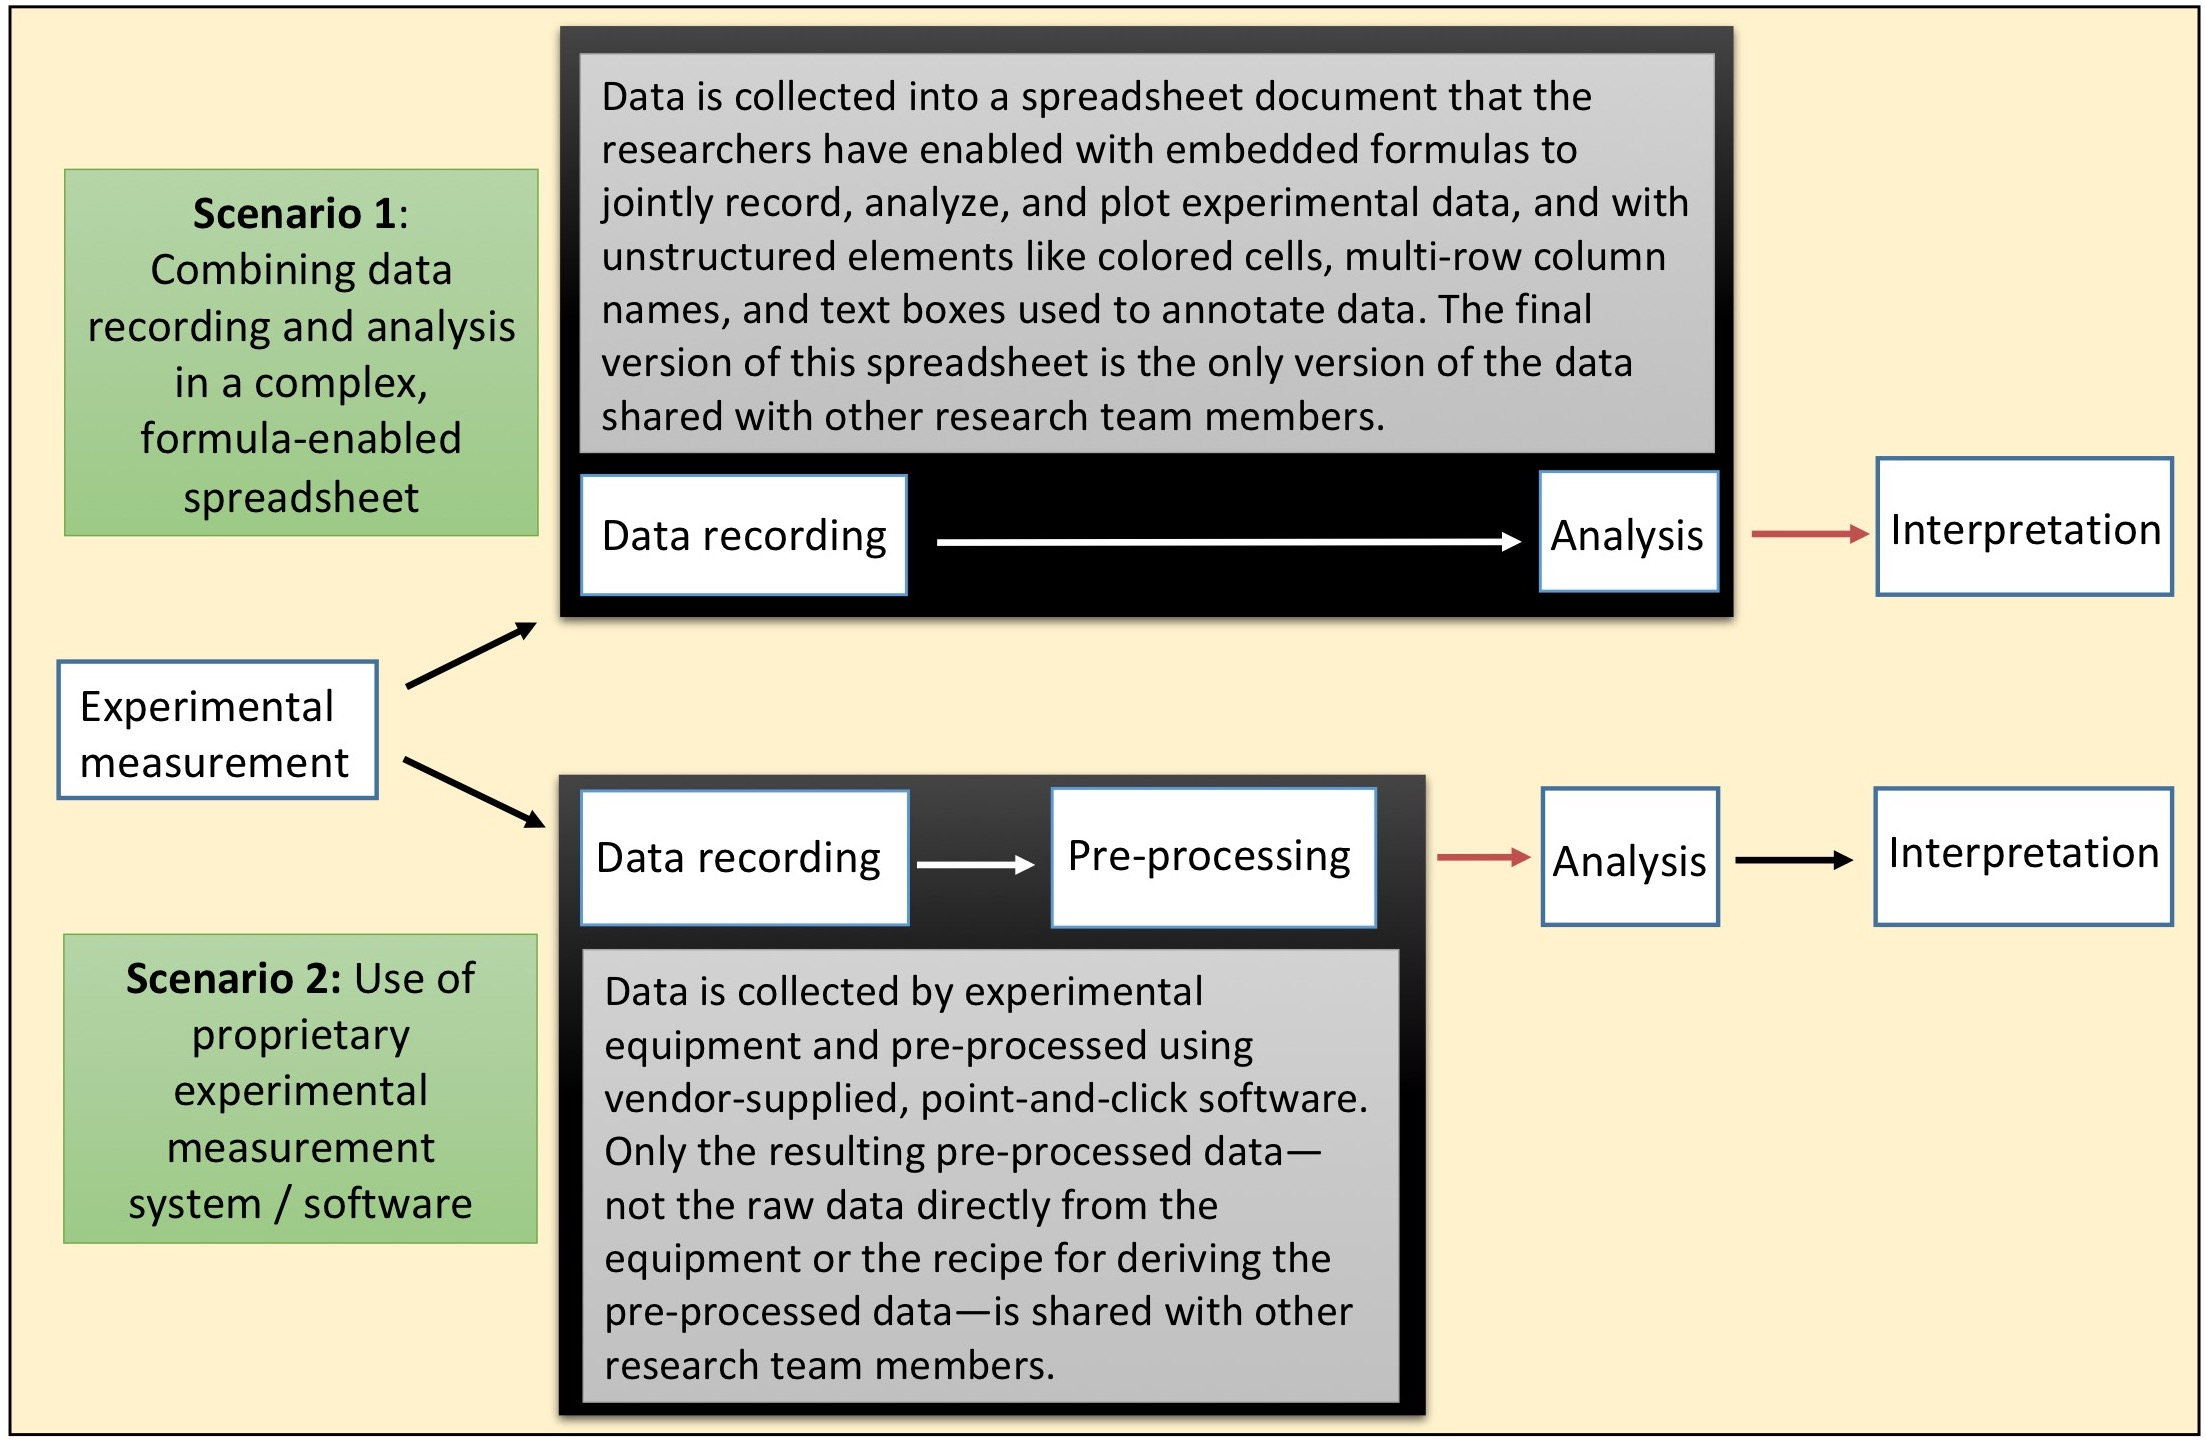
\includegraphics[width=\textwidth]{figures/existing_blackboxes} \caption[Two scenarios where 'black boxes' of non-transparent, non-reproducible data handling exist in research data workflows at the stages of data recording and pre-processing]{Two scenarios where 'black boxes' of non-transparent, non-reproducible data handling exist in research data workflows at the stages of data recording and pre-processing. These create potential points of failure for reproducible research. Red arrows indicate where data is passed to other research team members, including statisticians / data analysts, often within complex or unstructured spreadsheet files.}\label{fig:workflow}
\end{figure}

It is widely known and discussed among data scientists, mathematical modelers,
and statisticians \citep{broman2018data, krishnan2016towards} that there is
frequently a need to discard, transform, and reformat various elements of the
data shared with them by laboratory-based researchers, and that data is often
shared in an unstructured format, increasing the risks of introducing errors
through reformatting before applying more advanced computational methods.
Instead, a critical need for reproducibility is for the transparent and clear
sharing across research teams of: (1) raw data, directly from hand-recording or
directly output from experimental equipment; (2) data that has been
pre-processed as necessary (e.g., gating for flow cytometry data, feature
identification for metabolomics data), saved in a consistent, structured format,
and (3) a clear and repeatable description of how the pre-processed data was
generated from the raw data \citep{broman2018data, ellis2018share}.

To enhance data reproducibility, it is critical to create a clear separation
among data recording, data pre-processing, and data analysis---breaking up
commonly existing ``black boxes" in data handling across the research process.
Such a rigorous demarcation requires some change in the conventional
understanding and use of spreadsheets and a recognition by biomedical
researchers that recent advances in computer programming languages, especially
the R programming language, provide user-friendly and accessible tools and
concepts that can be used to extend a transparent and reproducible data workflow
to the steps of data recording and pre-processing. Among our team, we have found
that there are many common existing practices---including use of spreadsheets
with embedded formulas that concurrently record and analyze experimental data,
problematic management of project files, and reliance on proprietary,
vendor-supplied point-and-click software for data pre-processing---that can
interfere with the transparency, reproducibility, and efficiency of
laboratory-based biomedical research projects, problems that have also been
identified by others as key barriers to research reproducibility
\citep{broman2018data, bryan2018excuse, ellis2018share, marwick2018packaging}. In
these training modules, we have choosen topics that tackle barriers to
reproducibility that have straightforward, easy-to-teach solutions, but which
are still very common in biomedical laboratory-based research programs.

\hypertarget{license}{%
\section{License}\label{license}}

This book is licensed under the \href{https://creativecommons.org/licenses/by-nc-sa/4.0/}{Creative Commons
Attribution-NonCommercial-ShareAlike 4.0 International
License}, while all code in
the book is under the \href{https://opensource.org/licenses/MIT}{MIT license}.

Click on the \textbf{Next} button (or navigate using the
links at the top of the page) to continue.

\hypertarget{experimental-data-recording}{%
\chapter{Experimental Data Recording}\label{experimental-data-recording}}

This section includes modules on:

\begin{itemize}
\tightlist
\item
  \protect\hyperlink{module1}{Module 1: Separating data recording and analysis}
\item
  \protect\hyperlink{module2}{Module 2: Principles and power of structured data formats}
\item
  \protect\hyperlink{module3}{Module 3: The `tidy' data format}
\item
  \protect\hyperlink{module4}{Module 4: Designing templates for ``tidy'' data collection}
\item
  \protect\hyperlink{module5}{Module 5: Example: Creating a template for ``tidy'' data collection}
\item
  \protect\hyperlink{module6}{Module 6: Power of using a single structured `Project' directory for storing and tracking research project files}
\item
  \protect\hyperlink{module7}{Module 7: Creating `Project' templates}
\item
  \protect\hyperlink{module8}{Module 8: Example: Creating a `Project' template}
\item
  \protect\hyperlink{module9}{Module 9: Harnessing version control for transparent data recording}
\item
  \protect\hyperlink{module10}{Module 10: Enhance the reproducibility of collaborative research with version control platforms}
\item
  \protect\hyperlink{module11}{Module 11: Using git and GitLab to implement version control}
\end{itemize}

\hypertarget{module1}{%
\section{Separating data recording and analysis}\label{module1}}

Many biomedical laboratories currently use spreadsheet programs to jointly
record, visualize, and analyze experimental data \citep{broman2018data}. These
software tools, such as Microsoft Excel{[}Ref, copyright?{]} or Google Sheets{[}Ref,
copyright?{]}, provide for manual or automated entry of data into rows and columns
of cells. Standard or custom formulas and other operations can be applied to the
cells, and are commonly used to reformat or clean the data, calculate various
statistics, and to generate simple plots; all of which are embedded as
additional data entries and programming elements within the spreadsheet. While
these tools greatly improved the paper worksheets on which they were originally
based \citep{campbell2007number}, this all-in-one practice impedes the transparency
and reproducibility of both recording and analysis of the large and complex data
sets that are routinely generated in life science experiments.

To improve the computational reproducibility of a research project, it is
critical for biomedical researchers to learn the importance of maintaining
recorded experimental data as ``read-only'' files, separating data recording from
any data pre-processing or data analysis steps \citep{broman2018data, marwick2018packaging}. Statisticians have outlined specific methods that a
laboratory-based scientist can take to ensure that data shared in an Excel
spreadsheet are shared in a reliable and reproducible way, including avoiding
macros or embedded formulas, using a separate Excel file for each dataset,
recording descriptions of variables in a separate code book rather than in the
Excel file, avoiding the use of color of the cells to encode information, using
``NA'' to code missing values, avoiding spaces in column headers, and avoiding
splitting or merging cells \citep{ellis2018share, broman2018data}. In this module,
we will describe this common practice and will outline alternative approaches
that separate the steps of data recording and data analysis.

\textbf{Objectives.} After this module, the trainee will be able to:

\begin{itemize}
\tightlist
\item
  Explain the difference between data recording and data analysis
\item
  Understand why collecting data on spreadsheets with embedded formulas impedes
  reproducibility
\item
  List alternative approaches to improve reproducibility
\end{itemize}

\hypertarget{data-recording-versus-data-analysis}{%
\subsection{Data recording versus data analysis}\label{data-recording-versus-data-analysis}}

\textbf{History of spreadsheets.}

Spreadsheets have long been an extremely popular tool for recording and
analyzing data, in part because they allow people without programming experience
to conduct a range of standard computations and statistical analyses through a
visual interface that is more immediately user-friendly to non-programmers than
programs with command line interfaces. An early target for spreadsheet programs
in terms of users was business executives, and so the programs were designed to
be very simple and easy to use---just one step up in complexity from crunching
numbers on the back of an envelope \citep{campbell2007number}. Spreadsheet programs
in fact became so popular within businesses that many attribute these programs
with driving the uptake of personal computers \citep{campbell2007number}.

Spreadsheets were innovative and rapidly adapted in part because they allowed
users to combine data recording and analysis---while previously, in business
settings, any complicated data analysis task needed to be outsourced to
mainframe computers and data processing teams, the initial spreadsheet program
(VisiCalc) allowed one person to quickly apply and test different models or
calculations on recorded data \citep{levy1984spreadsheet}. These spreadsheet programs
allowed non-programmers to engage with data, including data processing and
analysis tasks, in a way that previously required programming expertise
\citep{levy1984spreadsheet}.

\textbf{Use of spreadsheets.}

Many scientific laboratories use spreadsheets within their data collection
process, both to record data and to clean and analyze the data. Illustrative
examples can be found in surveys of over 250 biomedical researchers at the University
of Washington \citep{anderson2007issues}, and of neuroscience researchers at the
University of Newcastle, with most respondents reporting the use of spreadsheets
and other general-purpose software in their research \citep{altarawneh2017pilot}.
A working group on bioinformatics and data-intensive science similarly found
spreadsheets were the most common tool used across attendees
\citep{barga2011bioinformatics}.

In some cases, a spreadsheet is used solely to record data, as a simple type of
database \citep{birch2018future}. However, biomedical researchers often use
spreadsheets to both record and analyze experimental data \citep{anderson2007issues}.
In this case, data processing and analysis is implemented through the use of
formulas and macros embedded within the spreadsheet. When a spreadsheet has
formulas or macros within it, the spreadsheet program creates an internal record
of how cells are connected through these formulas. For example, if the value in
a specific cell is converted from Fahrenheit to Celsius to fill a second cell,
and then that value is combined with other values in a column to calculate the
mean temperature across several observations, then the spreadsheet program has
internally saved how the later cells depend on the earlier ones. When you change
the value recorded in a cell of a spreadsheet, the spreadsheet program queries
this record and only recalculates the cells that depend on that cell. This
process allows the program to quickly ``react'' to any change in cell inputs,
immediately providing an update to all downstream calculations and analyses
\citep{levy1984spreadsheet}. Starting from the spreadsheet program Lotus 1-2-3,
spreadsheet programs also included \emph{macros}, ``a single computer instruction that
stands for a sequence of operations'' \citep{creeth1985microcomputer}.

Spreadsheets have become so popular in part because so many people know how to
use them, at least in basic ways, and so many people have the software on their
computers that files can be shared with the virtual guarantee that everyone will
be able to open the file on their own computer \citep{hermans2016spreadsheets}.
Spreadsheets use the visual metaphore of a traditional gridded ledger sheet
\citep{levy1984spreadsheet}, providing an interface that is easy for users to
immediately understand and create a mental map of \citep{birch2018future, barga2011bioinformatics}. This visually clear interface also means that
spreadsheets can be printed or incorporated into other documents (Word files,
PowerPoint presentations) ``as-is'', as a workable and understandable table of
data values. In fact, some of the most popular plug-in software packages for the
early spreadsheet program Lotus 1-2-3 were programs for printing and publishing
spreadsheets \citep{campbell2007number}. This ``What You See Is What You Get''
interface was a huge advance from previous methods of data analysis for the
first spreadsheet program, VisiCalc, providing a ``window to the data'' that was
accessible to business executives and others without programming expertise
\citep{creeth1985microcomputer}. Several surveys of researchers have found that
spreadsheets were popular because of their simplicity and ease-of-use
\citep{anderson2007issues, altarawneh2017pilot, barga2011bioinformatics}. By
contrast, databases and scritped programming lanugages can be perceived as
requiring a cognitive load and lengthly training that is not worth the
investment when an easier tool is available \citep{hermans2016spreadsheets, anderson2007issues, myneni2010organization, barga2011bioinformatics, topaloglou2004biological}.

\hypertarget{hazards-of-combining-recording-and-analysis}{%
\subsection{Hazards of combining recording and analysis}\label{hazards-of-combining-recording-and-analysis}}

\textbf{Raw data often lost.}

One of the key tenets of ensuring that research is computationally reproducible
is to always keep a copy of all raw data, as well as the steps taken to get from
the raw data to a cleaned version of the data through to the results of data
analysis. However, maintaining an easily accessible copy of all original raw data
for a project is a common problem among biomedical researchers
\citep{goodman2014ten}, especially as team members move on from a laboratory group
\citep{myneni2010organization}.

The use of spreadsheets to jointly record and analyze data can contribute to
this problem. Spreadsheets allow for the immediate and embedded processing of
data. As a result, it may become very difficult to pull out the raw data
originally recorded in a spreadsheet. At the least, the combination of raw and
processed data in a spreadsheet makes it hard to identify which data points
within a spreadsheet make up the raw data and which are the result of processing
that raw data. One study of operational spreadsheets noted that:

\begin{quote}
``The data used in most spreadsheets is undocumented and there is no practical
way to check it. Even the original developer would have difficulty checking the
data.'' \citep{powell2009errors}
\end{quote}

Further, data in a spreadsheet is typically not saved as ``read-only'', so it is
possible for it to be accidentally overwritten: in situations where spreadsheets
are shared among multiple users, original cell values can easily be accidentally
written over, and it may not be clear who last changed a value, when it was
changed, or why \citep{altarawneh2017pilot}.

Finally, many spreadsheets use a proprietary format. In the development of
spreadsheet programs, this use of proprietary binary file formats helped a
software program keep users, increasing barriers for a user to switch to a new
program (since the new program wouldn't be able to read their old files)
\citep{campbell2007number}. However, this file format may be hard to open in the
future, as software changes and evolves \citep{michener2015ten}; by comparison, plain
text files should be widely accessible through general purpose tools---a text
editor is a type of software available on all computers, for
example---regardless of changes to proprietary software like Microsoft Excel.

\textbf{Opacity of analysis steps and potential for errors.}

Previous studies have found that errors are very common within spreadsheets
\citep{hermans2016spreadsheets}. For example, one study of 50 operational
spreadsheets found that about 90\% contained at least one error
\citep{powell2009errors}. In part, it is easier to make errors in spreadsheets and
harder to catch errors in later work with a spreadsheet because the formulas and
connections between cells aren't visible when you look at the
spreadsheet---they're behind the scenes \citep{birch2018future}. This makes it very
hard to get a clear and complete view of the pipeline of analytic steps in data
processing and analysis within a spreadsheet, or to discern how cells
are connected within and across sheets of the spreadsheet. As one early article on
the history of spreadsheet programs notes:

\begin{quote}
``People tend to forget that even the most elegantly crafted spreadsheet is a
house of cards, ready to collapse at the first erroneous assumption. The
spreadsheet that looks good but turns out to be tragically wrong is becoming
a familiar phenomenon.'' \citep{levy1984spreadsheet}
\end{quote}

Some characteristics of spreadsheets may heighten chances for errors. These
include high conditional complexity (i.e., lots of branching of data flow
through if / else structures), formulas that depend on a large number of cells
or that incorporate many functions \citep{hermans2016spreadsheets}. Following the
logical chain of spreadsheet formulas can be particularly difficult when several
calculations are chained in a row \citep{hermans2015enron}. Very long chains of
dependent formulas across spreadsheet cells may in some case requiring sketching
out by hand the flow of information through the spreadsheet to understand what's
going on \citep{nardi1990spreadsheet}. The use of macros can also make it
particularly hard to figure out the steps of an analysis and to diagnose and fix
any bugs in those steps \citep{nash2006spreadsheets, creeth1985microcomputer}. One
study of spreadsheets used in real life applications noted that, ``Many
spreadsheets are so chaotically designed that auditing (especially of a few
formulas) is extremely difficult or impossible.'' \citep{powell2009errors}

In some cases, formula dependences might span across different sheets of a
spreadsheet file. For the example given previously of a spreadsheet that converts
temperature from one unit to another and then averages across observations, for
example, the original temperature might be recorded in one sheet while the
converted temperature value is calculated and shown in a second sheet. These
cross-sheet dependencies can make the analysis steps even more opaque
\citep{hermans2016spreadsheets}, as a change in the cell value of one sheet might not
be immediately visible as a change in another cell on that sheet (the same is
true for spreadsheets so large that all the cells in a sheet are not
concurrently visible on the screen). Other common sources of errors included
incorrect references to cells inside formulas and incorrect use of formulas
\citep{powell2009errors} or errors introduced through the common practice of copying
and pasting when developing spreadsheets \citep{hermans2016spreadsheets}.

To keep analysis steps clear, whether in scripted code or in spreadsheets or
pen-and-paper calculations, it is important to document what is being done at
each step and why \citep{goodman2014ten}. Scripted languages allow for code comments,
which are written directly into the script but not evaluated by the computer,
and so can be used to document steps within the code without changing the
operation of the code. Further, the program file itself often presents a linear,
step-by-step view of the pipeline, stored separated from the data itself
\citep{creeth1985microcomputer}. Calculations done with pen-and-paper (e.g., in a
laboratory notebook) can be annotated with text to document the steps.
Spreadsheets, on the other hand, are often poorly documented, or documented in
ways that are hard to keep track of. Before spreadsheets,

\begin{quote}
``The formulas appeared in one place and the results in another. You could see
what you were getting. That cannot be said of electronic spreadsheets, which
don't display the formulas that govern their calculations. As Mitch Kapor
explained, with electronic spreadsheets, `You can just randomly make formulas,
all of which depend on each other. And when you look at the final results, you
have no way of knowing what the rules are, unless someone tells you.'\,''
\citep{levy1984spreadsheet}
\end{quote}

Within spreadsheets, the logic and methods behind the pipeline of data
processing and analysis is often not documented, or only documented with cell
comments (hard to see as a whole) or in emails, not the spreadsheet file.
One study that investigated a large collection of spreadsheets found that most
do not include documentation explaining the logic or implementation of data
processing and analysis implemented within the spreadsheet
\citep{hermans2016spreadsheets}. A survey of neuroscience researchers at a UK
institute found that about a third of respondents included no documentation
for spreadsheets used in their research laboratories \citep{altarawneh2017pilot}.

When spreadsheet pipelines are documented, it is often through methods that are
hard to find and interpret later. One study of scientific researchers found
that, when research spreadsheets were documented, it was often through ``cell
comments'' added to specific cells in the spreadsheet, which can be hard to
interpret inclusively to understand the flow and logic of a spreadsheet as a
whole \citep{altarawneh2017pilot}. In some cases, teams discuss and document
functionality and changes in spreadsheets through email chains, passing
different versions of the spreadsheet file as attachments of emails with
discussion of the spreadsheet in the email body. One research team investigated
over 700,000 emails from employees of Enron that were released during legal
proceedings and investigated the spreadsheets attached to these emails (over
15,000 spreadsheets) as well as discussion of the spreadsheets within the emails
themselves \citep{hermans2015enron}. They found that the logic and methods of
calculations within the spreadsheets were often documented within the bodies of
emails that team members used to share and discuss spreadsheets. This means
that, if someone needs to figure out why a step was taken or identify when an
error was introduced into a spreadsheet, they may need to dig through the chain
of old emails documenting that spreadsheet, rather than being able to find the
relevant documentation within the spreadsheet's own file.

Often spreadsheets are designed, and their structure determined, by one person,
and this is often done in an \emph{ad hoc} fashion, rather than designing the
spreadsheet to follow a common structure for the research field or for the
laboratory group \citep{anderson2007issues}. Often, data processing and analysis
pipelines for spreadsheets are not carefully designed; instead, it's more
typically for spreadsheet user to start by directly entering data and formulas
without a clear overall plan \citep{altarawneh2017pilot}. Often, the person who
created the spreadsheet is the only person who fully knows how it works
\citep{myneni2010organization}, particularly if the spreadsheet includes complex
macros or a complicated structure in the analysis pipeline
\citep{creeth1985microcomputer}.

This practice creates a heavy dependence on the person who created that
spreadsheet anytime the data or results in that spreadsheet need to be
interpreted. This is particularly problematic in projects where the spreadsheet
will be shared for collaboration or adapted to be used in a future project, as
is often done in scientific research groups. One survey of neuroscience
researchers at a UK institute, for example, found that ``on average, 2--5
researchers share the same spreadsheet''. \citep{altarawneh2017pilot} In this case, it
can be hard to ``onboard'' new people to use the file, and much of the work and
knowledge about the spreadsheet can be lost when that person moves on from the
business or laboratory group \citep{creeth1985microcomputer, myneni2010organization}. If you share a spreadsheet with numerous and complex
macros and formulas included to clean and analyze the data, it can take an
extensive amount of time, and in some cases may be impossible, for the
researcher you share it with to decipher what is being done to get from the
original data input in some cells to the final results shown in others and in
graphs. Further, if others can't figure out the steps being done through macros
and formulas in a spreadsheet, they will not be able to check it for problems in
the logic of the overall analysis pipeline or for errors in the specific
formulas used within that pipeline. They also will struggle to extend and adapt
the spreadsheet to be used for other projects. These problems come up not only
when sharing with a collaborator, but also when reviewing spreadsheets that you
have previously created and used (as many have noted, your most frequent
collaborator will likely be ``future you''). In fact, one survey of biomedical
researchers at the University of Washington noted that,

\begin{quote}
``The profusion of individually created spreadsheets containing overlapping and
inconsistently updated data created a great deal of confusion within some labs.
There was little consideration to future data exchange of submission
requirements at the time of publication.'' \citep{anderson2007issues}
\end{quote}

There are methods that have been brought from more traditional programming work
into spreadsheet programming to try to help limit errors, including a tool
called assertions that allows users to validate data or test logic within their
spreadsheets \citep{hermans2016spreadsheets}. However, these are often not
implemented, in part perhaps because many spreadsheet users see themselves as
``end-users'', creating spreadsheets for their own personal use rather than as
something robust to future use by others, and so don't seek out strategies
adopted by ``programmers'' when creating stable tools for others to use
\citep{hermans2016spreadsheets}. In practice, though, often a spreadsheet is used
much longer, and by more people, than originally intended. From early in the
history of spreadsheet programs, users have shared spreadsheet files with
interesting functionality with other users \citep{levy1984spreadsheet}, and the
lifespan of a spreadsheet can be much longer than originally intended---a
spreadsheet created by one user for their own personal use can end up being used
and modified by that person or others for years \citep{hermans2016spreadsheets}.

\textbf{Subpar software for analysis.}

While spreadsheets serve as a widely-used tool for data recording and analysis,
in many cases spreadsheets programs are poorly suited to clean and analyze
scientific data compared to other programs. As tools and interfaces continue to
develop that make other software more user-friendly to those new to programming,
scientists may want to reevaluate the costs and benefits, in terms of both time
required for training and aptness of tools, for spreadsheet programs compared to
using scripted programming languages like R and Python.

Several problems have been identified with spreadsheet programs in the context of
recording and, especially, analyzing scientific data. First, some statistical
methods may be inferior to those available in other statistical programming language.
Since the most popular spreadsheet program (Excel) is closed source, it is hard to
identify and diagnose such problems, and there is likely less of an incentive for
problems in statistical methodology to be fixed (rather than using development time
and funds to increase easier-to-see functionality in the program). Many statistical
operations require computations that cannot be perfectly achieved with a
computer, since the computer must ultimately solve many mathematical problems using
numerical approximations rather than continuous methods (e.g., calculus). The choice of
the algorithms used for these approximations heavily influence how closely a result
approximates the true answer.

A series of papers examined the quality of statistical methods in several
statistical software programs, including Excel, starting in the 1990s
\citep{mccullough1999accuracy, mccullough1999assessing, mccullough2002accuracy, mccullough2005accuracy, mccullough2008accuracy, melard2014accuracy}. In the
earliest studies, they found some concerns across all programs considered
\citep{mccullough1999accuracy, mccullough1999assessing}. One of the biggest
concerns, however, was that there was little evidence over the years that the
identified problems in Excel were resolved, or at least improved, over time
\citep{mccullough2001does, mccullough2008accuracy}. The authors note that there may
be little incentive for checking and fixing problems with algorithms for
statistical approximation in closed source software like Excel, where sales
might depend more on the more immediately evident functionality in the software,
while problems with statistical algorithms might be less evident to potential
users \citep{mccullough2001does}.

Open source software, on the other hand, offers pathways for identifying and fixing
any problems in the software, including for statistical algorithms and methods
implemented in the software's code. Since the full source code is available, researchers
can closely inspect the algorithms being used and compare them to the latest
knowledge in statistical computing methodology. Further, if an inferior algorithm is in
use, most open source software licenses allow a user to adapt and extend the software,
for example to implement better statistical algorithms.

Second, spreadsheet programs can include automated functionality that's meant to
make something easier for most users, but that might invisibly create problems
in some cases. A critical problem, for example, has been identified when using
Excel for genomics data. When Excel encounters a cell value in a format that
seems like it could be a date (e.g., ``Mar-3-06''), it will try to convert that
cell to a ``date'' class. Many software programs save date as this special ``date''
format, where it is printed and visually appears in a format like ``3-Mar-06'' but
is saved internally by the program as a number (for Microsoft Excel, the number
of days since January 1, 1900 \citep{willekens2013chronological}). By doing this, the
software can more easily undertake calculations with dates, like calculating the
number of days between two dates or which of two dates is earlier.
Bioinformatics researchers at the National Institutes of Health found that Excel
was doing this type of automatic and irreversible date conversion for 30 gene
names, including ``MAR3'' and ``APR-4'', resulting in these gene names being lost
for further analysis \citep{zeeberg2004mistaken}.

Avoiding this automatic date conversion required specifying that columns with
columns susceptible to these problems, including columns of gene names, should
be retained in a ``text'' class in Excel's file import process. While this
problem was originally identified and published in 2004 \citep{zeeberg2004mistaken},
along with tips to identify and avoid the problem, a study in 2016 found that
approximately a fifth of genomics papers investigated in a large-scale review
had gene name errors resulting from Excel automatic conversion, with the rate of
errors actually increasing over time \citep{ziemann2016gene}.

Other automatic conversion problems caused the lost of clone identifiers with
composed of digits and the letter ``E'' \citep{zeeberg2004mistaken, welsh2017escape},
which were assumed to be expressing a number using scientific notation and so
automatically and irreversibly converted to a numeric class. Further automatic
conversion problems can be caused by cells that start with an operator (e.g., ``+
control'') or with leading zeros in a numeric identifier (e.g., ``007'')
\citep{welsh2017escape}.

Finally, spreadsheet programs can be limited as analysis needs become more
complex or large \citep{topaloglou2004biological}. For example, spreadsheets can be
problematic when integrating or merging large, separate datasets
\citep{birch2018future}. This can create barriers, for example, in biological studies
seeking to integrate measurements from different instruments (e.g., flow
cytometry data with RNA-sequencing data). Further, while spreadsheet programs
continue to expand in their capacity for data, for very large datasets they
continue to face limits that may be reached in practical applications
\citep{birch2018future}---until recently, for example, Excel could not handle more
than one million rows of data per spreadsheet. Even when spreadsheets can handle
larger data, their efficiency in running data processing and analysis pipelines
across large datasets can be slow compared to code implemented with other
programming languages.

\textbf{Difficulty collaborating with statisticians.}

Modern biomedical researchers requires large teams, with statisticians and
bioinformaticians often forming a critical part of the team to enable
sophisticated processing and analysis of experimental data. However, the process
of combining data recording and analysis of experimental data, especially
through the use of spreadsheet programs, can create barriers in working across
disciplines. One group defined these issues as ``data friction'' and ``science
friction''---the extra steps and work required at each interface where data
passes, for example, from a machine to analysis or from a collaborator in one
discipline to one in a separate discipline \citep{edwards2011science}.
From a survey of scientific labs, for example, one respondent said:

\begin{quote}
``I can give data that I think are appropriate to answer a question to a
biostatistician, but when they look at it, they see it from a different point of
view. And that spreadsheet does not really encapsulate where it came from very
well, how was it generated, was it random, how was this data collected. You
would run a series of queries that you think are pertinent to what this
biostatistician would want to know. They become a part of the exploration and
not just a receiver of whatever I decided to put in my spreadsheet on that day.
What I get back is almost never fully documented in any way that I can really
understand and add more to the process.'' \citep{myneni2010organization}
\end{quote}

When collaborating with statisticians or bioinformaticians, one of the key
sources of this ``data friction'' can result from the use of spreadsheets to
jointly record and analyze experiemental data. First, spreadsheets are easy to
print or copy into another format (e.g., PowerPoint presentation, Word
document), and so researchers often design spreadsheets to be immediately
visually appealing to viewers. For example, a spreadsheet might be designed to
include hierarchically organized headers (e.g., heading and subheading, some
within a cell merged across several columns), or to show the result of a
calculation at the bottom of a column of observations (e.g., ``Total'' in the last
cell of the column) \citep{teixeira2016emergence}. Multiple separate small tables
might be included in the same sheet, with empty cells used for visual
separation, or use a ``horizontal single entry'' design , where the headers are in
the leftmost column rather than the top row \citep{teixeira2016emergence}.

These spreadsheet design choices make it much more difficult for the contents of
the spreadsheet to be read into other statistical programs. These types of data
require several extra steps in coding, in some cases fairly complex coding, with
regular expressions or logical rules needed to parse out the data and convert it
to the needed shape, before the statistical work can be done for the dataset.
This is a poor use of time for a collaborating statistician, especially if it
can be avoided through the design of the data recording template. Further, it
introduces many more chances for errors in cleaning the data.

Further, information embedded in formulas, macros, and extra formatting like
color or text boxes is lost when the spreadsheet file is input into other
programs. Spreadsheets allow users to use highlighting to represent information
(e.g., measurements for control animals shown in red, those for experiment
animals in blue) and to include information or documentation in text boxes. For
example, one survey study of biomedical researchers at the University of
Washington included this quote from a respondent: ``I have one spreadsheet that
has all of my chromosomes \ldots{} and then I've gone through and color coded it for
homozygosity and linkage.'' \citep{anderson2007issues} All the information encoded in
this sheet through color will be lost when the data from the spreadsheet is read
into another statistical program.

\hypertarget{approaches-to-separate-recording-and-analysis}{%
\subsection{Approaches to separate recording and analysis}\label{approaches-to-separate-recording-and-analysis}}

In the remaining modules in this section, we will present and describe techniques
that can be used to limit or remove these problems. First, in the module on
``Structured data'', we will walk through techniques to design data recording
formats so that data is saved in a consistent format across experiments within
a laboratory group, and in a way that removes ``data friction'' for collaboration
with statisticians or later use in scripted code. These techniques can be immediately
used to design a better spreadsheet to be used solely for data collection.

In later modules, we will discuss the use of R projects to coordinate data
recording and analysis steps within a directory, while using separate files for
data recording versus data processing and analysis. These more advanced formats
will enable the use of quality assurance / control measures like testing of data
entry and analysis functionality, better documentation of data analysis pipelines,
and easy use of version control to track projects and collaborate transparently and
with a recorded history.

{[}We will probably want to flesh this section out as we write later modules.{]}

\hypertarget{discussion-questions}{%
\subsection{Discussion questions}\label{discussion-questions}}

\hypertarget{module2}{%
\section{Principles and power of structured data formats}\label{module2}}

The format in which experimental data is recorded can have a large influence on
how easy and likely it is to implement reproducibility tools in later stages of
the research workflow. Recording data in a ``structured'' format brings many
benefits. In this module, we will explain what makes a dataset ``structured'' and
why this format is a powerful tool for reproducible research.

Every extra step of data cleaning is another chance to introduce errors in
experimental biomedical data, and yet laboratory-based researchers often share
experimental data with collaborators in a format that requires extensive
additional cleaning before it can be input into data analysis
\citep{broman2018data}. Recording data in a ``structured'' format brings many
benefits for later stages of the research process, especially in terms of
improving reproducibility and reducing the probability of errors in analysis
\citep{ellis2018share}. Data that is in a structured, tabular, two-dimensional
format is substantially easier for collaborators to understand and work with,
without additional data formatting \citep{broman2018data}. Further, by using a
consistent structured format across many or all data in a research project, it
becomes much easier to create solid, well-tested code scripts for data
pre-processing and analysis and to apply those scripts consistently and
reproducibly across datasets from multiple experiments \citep{broman2018data}.
However, many biomedical researchers are unaware of this simple yet powerful
strategy in data recording and how it can improve the efficiency and
effectiveness of collaborations \citep{ellis2018share}.

\textbf{Objectives.} After this module, the trainee will be able to:

\begin{itemize}
\tightlist
\item
  List the characteristics of a structured data format
\item
  Describe benefits for research transparency and reproducibility
\item
  Outline other benefits of using a structured format when recording data
\end{itemize}

\hypertarget{data-recording-standards}{%
\subsection{Data recording standards}\label{data-recording-standards}}

For many areas of biological data, there has been a push to create standards for
how data is recorded and communicated. Standards can clarify both the \emph{content}
that should be included in a dataset, the \emph{format} in which that content is
stored, and the \emph{vocabulary} used within this data. One article names these three
facets of a data standard as the \textbf{minimum information}, \textbf{file formats}, and
\textbf{ontologies} \citep{ghosh2011software}.

\begin{quote}
``It is important to distinguish between standards that specify how to actually
do experiments and standards that specify how to describe experiments.
Recommendations such as what standard reporters (probes) should be printed on
microarrays or what quality control steps should be used in an experiment belong
to the first category. Here we focus on the standards that specify how to
describe and communicate data and information.'' \citep{brazma2006standards}
\end{quote}

Many people and organizations (including funders) are excited about the idea
of developing and using data standards, especially at the community level.
Good standards, that are widely adapted by researchers, can help in making
sure that data submitted to data repositories are used widely and that software
can be developed that is \emph{interoperable} with data from many research group's
experiments. There are also many advantages, if there are not community-level
standards for recording a certain type of data, to develop and use local
data standards for recording data from your own experiments. This section
describes the elements that go into a data standard, discusses some choices
to be made when definining a data standard (especially choices on data
structure and file formats), and some of the advantages and disadvantages
of developing and using data recording standards at both the research group
and community levels.

\begin{quote}
The first of four root causes for irreproducibility in biomedical research: ``First,
a lack of standards for data generation leads to problems with the comparability
and integration of data sets.'' \citep{waltemath2016modeling}
\end{quote}

\textbf{Ontology standards.} Although it has the most complex name, an \emph{ontology}
(sometimes called a \emph{terminology} \citep{sansone2012toward}) might be the easiest and
quickest to adapt in recording data. An ontology helps define a vocabulary that
is controlled and consistent to use that researchers can use to refer to
concepts and concrete things within an area of research. It helps researchers,
when they want to talk about an idea or thing, to use one word, and just one
word, and to ensure that it will be the same word used by other researchers when
they refer to that idea or thing. Ontologies also help to define the relationships
between ideas or concrete things in a research area \citep{ghosh2011software}, but
here we'll focus on their use in provided a consistent vocabulary to use when
recording data.

For example, when recording a dataset, what do you call a small mammal that is
often kept as a pet and that has four legs and whiskers and purrs? Do you record
this as ``cat'' or ``feline'' or maybe, depending on the animal, even ``tabby'' or
``tom'' or ``kitten''? Similarly, do you record tuberculosis as ``tuberculosis'' or
``TB'' or or maybe even ``consumption''? If you do not use the same word
consistently in a dataset to record an idea, then while a human might be able to
understand that two words should be considered equivalent, a computer will not
be able to immediately tell that ``TB'' should be treated equivalently to
``tuberculosis''.

At a larger scale, if a research community can adapt an ontology they agree to
use throughout their studies, it will make it easier to understand and integrate
datasets produced by different research laboratories. If every research group
uses the term ``cat'', then code can easily be written to extract and combine
all data recorded for cats across a large repository of experimental data.
On the other hand, if different terms are used, then it might be necessary to
first create a list of all terms used in datasets in the respository, then pick
through that list to find any terms that are exchangeable with ``cat'', then write
script to pull data with any of those terms.

Several onotologies already exist or are being created for biological and other
biomedical research \citep{ghosh2011software}. Existing community-level ontologies in
the biological sciences include {[}Gene Ontology and Systems Biology Ontology are
listed in the Ghosh et al.~paper as two examples{]}. For biomedical science,
practice, and research, the BioPortal website
(\url{http://bioportal.bioontology.org/}) provides access to almost 800 ontologies,
including several versions of the International Classification of Diseases, the
Medical Subject Headings (MESH), the National Cancer Institute Thesaurus, the
Orphanet Rare Disease Ontology and the National Center for Biotechnology
Information (NCBI) Organismal Classification. For each ontology in the BioPortal
website, the website provides a link for downloading the ontology in several
formats. If you download the ontology as a ``CSV'', you can open it in your
favorite spreadsheet program and explore how it defines specific terms to use
for each idea or thing you might need to discuss within that topic area, as well
as synonyms for some of the terms. To use an ontology when recording your own
data, just make sure you use the ontology's suggested terms in your data. For
example, if you'd like to use the Ontology for Biomedical Investigations
(\url{http://bioportal.bioontology.org/ontologies/OBI}) and you are recording how many
children a woman has had who were born alive, you should name that column of the
data ``number of live births'', not ``\# live births'' or ``live births (N)'' or
anything else. Other collections of ontologies exist for fields of scientific
research, including the Open Biological and Biomedical Ontology (OBO) Foundry
(\url{http://www.obofoundry.org/}).

If there are community-wide ontologies in your field, it is worthwhile to use
them in recording experimental data in your research group. Even better is to
not only consistently use the defined terms, but also to follow any conventions
with capitalization. While most statistical programs provide tools to change
capitalization (for example, to change all letters in a character string to
lower case), this process does require an extra step of data cleaning and an
extra chance for confusion or for errors to be introduced into data.

\textbf{Minimum information standards.} The next easiest facet of a data standard to
bring into data recording in a research group is \emph{minimum information}. Within a
data recording standard, \emph{minimum information} (sometimes also called \emph{minimum
reporting guidelines} \citep{sansone2012toward} or \emph{reporting requirements}
\citep{brazma2006standards}) specify \emph{what} should be included in a dataset
\citep{ghosh2011software}. Using minimum information standards help ensure that data
within a laboratory, or data posted to a repository, contain a number of
required elements. This makes it easier to re-use the data, either to compare it
to data that a lab has newly generated, or to combine several posted datasets to
aggregate them for a new, integrated analysis, considerations that are growing
in importance with the increasing prevalence of research repositories and
research consortia in many fields of biomedical science \citep{keller2017evolution}.

\begin{quote}
``Minimum information is a checklist of required supporting information for
datasets from different experiments. Examples include: Minimum Information About
a Microarray Experiment (MIAME), Minimum Information About a Proteomic
Experiment (MIAPE), and the Minimum Information for Biological and Biomedical
Investigations (MIBBI) project.'' \citep{ghosh2011software}
\end{quote}

\emph{Standardized file formats.} While using a standard ontology and a standard for
minimum information is a helpful start, it just means that each dataset has the
required elements \emph{somewhere}, and using a consistent vocabulary---it doesn't
specify where those elements are in the data or that they'll be in the same
place in every dataset that meets those standards. As a result, datasets that all
meet a common standard can still be very hard to combine, or to create common
data analysis scripts and tools for, since each dataset will require a different
process to pull out a given element.

Computer files serve as a way to organize data, whether that's recorded
datapoints or written documents or computer programs \citep{kernighan1984unix}. As
the programmer Paul Ford writes,

\begin{quote}
``Data is just stuff, or rather, structured stuff: The cells of a spreadsheet,
the structure of a Word document, computer programs themselves---all data.''
\citep{ford2015i}
\end{quote}

\noindent A \emph{file format} defines the rules for how the bytes in the chunk of
memory that makes up a certain file should be parsed and interpreted anytime you
want to meaningfully access and use the data within that file
\citep{murrell2009introduction}. There are many file formats you may be familiar
with---a file that ends in ``.pdf'' must be opened with a Portable Document Format
(PDF) Reader like Adobe Acrobat, or it won't make much sense (you can try this
out by trying to open a ``.pdf'' file with a text editor, like TextEdit or
Notepad). The Reader has been programmed to interpret the data in a ``.pdf'' file
based on rules defining what data is stored where in the section of computer
memory for that file. Because most ``.pdf'' files conform to the same \emph{file
format} rules, powerful software can be built that works with any file in that
format.

For certain types of biomedical data, the challenge of standardizing a format
has similarly been addressed through the use of well-defined rules for not only
the content of data, but also the way that content is \emph{structured}. This can be
standardized through \emph{standardized file formats} (sometimes also called \emph{data
exchange formats} \citep{brazma2006standards}) and often defines not only the
upper-level file format (e.g., use of a ``.csv'' file type), but also how data
within that file type should be organized. If data from different research
groups and experiments is recorded using the same file format, researchers can
develop software tools that can be repeatedly used to interpret and visualize
that data; on the other hand, if different experiments record data using
different formats, bespoke analysis scripts must be written for each separate
dataset. This is a blow not only to the efficiency of data analysis, but also a
threat to the accuracy of that analysis. If a set of tools can be developed that
will work over and over, more time can be devoted to refining those tools and
testing them for potential errors and bugs, while one-shot scripts often can't
be curated with similar care. One paper highlights the dangers that come with
working with files that don't follow a defined format:

\begin{quote}
``Beware of common pitfalls when working with \emph{ad hoc} bioinformatics formats.
Simple mistakes over minor details like file formats can consume a
disproportionate amount of time and energy to discover and fix, so mind these
details early on.'' \citep{buffalo2015bioinformatics}
\end{quote}

Some biomedical data file formats have been created to help smooth over the
transfer of data that's captured by complex equipment into software that can
analyze that data. For example, many immunological studies need to measure
immune cell populations in experiments, and to do so they use piece of
equipment called a flow cytometer that probes cells in a sample with lasers
and measures resulting intensities to determine characteristics of that cell.
The data created by this equipment is large (often measurements from {[}x{]} or more
lasers are taken for {[}x{]} cells in a single run) and somewhat complex, with a need
to record not only the intensity measurements from each laser, but also some metadata
about the equipment and characteristics of the run.
If every company that manufactured flow cytometers used a different file format for
saving the resulting data, then a different set of analysis software would need to
be developed to accompany each piece of equipment. For example, a laboratory at
a university with flow cytometers from two different companies would need licenses
for two different software programs to work with data recorded by flow cytometers,
and they would need to learn how to use each software package separately. There is a
chance that software could be developed that used shared code for data analysis, but only
if it also included separate sets of code to read in data from all types of equipment
and to reformat them to a common format.

This isn't the case, however. Instead, there is a commonly agreed on file
format that flow cytometers should use to record the data they collect, called
the the \emph{FCS file format}. This format has been defined through a series of
papers {[}refs{]}, with several separate versions as the file format has evolved
over the years. It provides clear specifications on where to save each relevant
piece of information in the block of memory devoted to the data recorded by the
flow cytometer (in some cases, leaving a slot in the file blank if no relevant
information was collected on that element). As a result, people have been able
to create software, both proprietary and open-source, that can be used with any
data recorded by a flow cytometer, regardless of which company manufacturer the
piece of equipment that was used to generate the data. Other types of biomedical
data also have standardized file formats, including {[}example popular file
formats for biomedical data{]}. In some cases these were defined by an
organization, society, or initiative (e.g., the Metabolomics Standards
Initiative) \citep{ghosh2011software}, while in some cases the file format developed
by a specific equipment manufacturer has become popular enough that it's
established itself as the standard for recording a type of data
\citep{brazma2006standards}.

For an even simpler example, thing about recording dates. The \emph{minimum
information standard} for a date might always be the same---a recorded value
must include the day of the month, month, and year. However, this information
can be \emph{structured} in a variety of ways. In many scientific data, it's common
to record this information going from the largest to smallest units, so March
12, 2006, would be recorded ``2006-03-12''. Another convention (especially in the
US) is to record the month first (e.g., ``3/12/06''), while another (more common
in Europe) is to record the day of the month first (e.g., ``12/3/06'').

If you are trying to combine data from different datasets with dates, and all
use a different structure, it's easy to see how mistakes could be introduced
unless the data is very carefully reformatted. For example, March 12 (``3-12''
with month-first, ``12-3'' with day-first) could be easily mistaken to be December
3, and vice versa. Even if errors are avoided, combining data in different
structures will take more time than combining data in the same structure,
because of the extra needs for reformatting to get all data in a common
structure.

\begin{quote}
``Vast swathes of bioscience data remain locked in esoteric formats, are
described using nonstandard terminology, lack sufficient contextual information,
or simply are never shared due to the perceived cost or futility of the
exercise.'' \citep{sansone2012toward}
\end{quote}

\hypertarget{defining-data-standards-for-a-research-group}{%
\subsection{Defining data standards for a research group}\label{defining-data-standards-for-a-research-group}}

If some of the data you record from your experiments comes from complex
equipment, like flow cytometers {[}or?{]}, you may be recording much of that data in
a standardized format without any extra effort, because that format is the
default output format for the equipment. However, you may have more control over
other data recorded from your experiments, including smaller, less complex data
recorded directly into a laboratory notebook or spreadsheet. You can derive a
number of benefits from defining and using a standard for collecting this data,
as well.

As already mentioned, for many of the complex types of biological data,
standardized file formats exist. For example, flow cytometry data is typically
collected and recorded in \emph{.fcs} files. Every piece of flow cytometry equipment
can then be built to output data in this format, and every piece of software to
analyze flow cytometry data can be built to read in this input. The \emph{.fcs} file
format species how both raw data and metadata (e.g., compensation information,
equipment details) can be saved within the file---everyone who uses that file
format knows where to store data and where to find data of a certain type.

Much of the data collected in a laboratory is smaller, less complex, or less
structured than these types of data, data that is recorded ``by hand'', often into
a laboratory notebook or a spreadsheet. One paper describes this type of data as
the output of ``traditional, low-throughput bench science'' \citep{wilkinson2016fair}.
For this data recording, the data may be written down in an \emph{ad hoc}
way---however the particular researcher doing the experiment thinks makes
sense---and that format might change with each experiment, even if many
experiments have similar data outputs. As a result, it becomes harder to create
standardized data processing and analysis scripts that work with this data or
that integrate it with more complex data types. Further, if everyone in a
laboratory sets up their spreadsheets for data recording in their own way, it is
much harder for one person in the group to look at data another person recorded
and immediately find what they need within the spreadsheet.

As a step in a better direction, the head of a research group may
designate some common formats (e.g., a spreadsheet template) that all
researchers in the group should use when recording the data from a specific type
of experiments. This provides consistency across the recorded data for the
laboratory, making easier for one lab member to quickly understand and navigate
data saved by another lab member. It also opens the possibility to create tools
or scripts that read in and analyze the data that can be re-used across multiple
experiments with minor changes. This helps improve the efficiency and
reproducibility of data analysis, visualization, and reporting steps of the
research project.

This does require some extra time commitment \citep{brazma2006standards}. First, time
is needed to design the format, and it does take a while to develop a format
that is inclusive enough that it includes a place to put all data you might want
to record for a certain type of experiment. Second, it will take some time to
teach each laboratory member what the format is and how to make sure they comply
with it when they record data.

On the flip side, the longer-term advantages of using a defined, structured
format will outweigh the short-term time investments for many laboratory groups
for frequently used data types. By creating and using a consistent structure to
record data of a certain type, members of a laboratory group can increase their
efficiency (since they do not need to re-design a data recording structure
repeatedly). They can also make it easier for downstream collaborators, like
biostatisticians and bioinformaticians, to work with their output, as those
collaborators can create tools and scripts that can be recycled across
experiments and research projects if they know the data will always come to them
in the same format. These benefits increase even more if data format standards
are created and used by a whole research field (e.g., if a standard data
recording format is always used for researchers conducting a certain type of
drug development experiment), because then the tools built at one institution
can be used at other insitutions. However, this level of field-wide coordination
can be hard to achieve, and so a more realistic immediate goal might be
formalizing data recording structures within your research group or department,
while keeping an eye out for formats that are gaining popularity as standards in
your field to adopt within your group.

One key advantage to using standardized data formats even for recording simple,
``low-throughput'' data is that everyone in the research group will be able to
understand and work with data recorded by anyone else in the group---data will
not become impenetrable once the person who recorded it leaves the group. Also,
once a group member is used to the format, the process of setting up to record
data from a new experiment will be quicker, as it won't require the effort of
deciding and setting up a \emph{de novo} format for a spreadsheet or other recording
file. Instead, a template file can be created that can be copied as a starting
point for any new data recording.

Finally, there are huge benefits further down the data analysis pipeline that
come with always recording data in the same format. If your group is working
with a statistician or data analyst, it becomes much easier for that person to
quickly understand a new file if it follows the same format as previous files.
Further, if you work with a statistician or data analyst, he or she probably
creates code scripts to read in, re-format, analyze, and visualize the data
you've shared. If you always record data using the same format, these scripts
can be reused with very little modification. This saves valuable time, and it
helps make more time for more interesting statistical analysis if your
collaborator can trim time off reading in and reformatting the data in their
statistical programming language.

One paper suggests that the balance can be found, in terms of deciding whether
the benefits of developing a standard outweigh the costs, by considering how
often data of a certain type is generated and used:

\begin{quote}
``To develop and deploy a standard creates an overhead, which can be expensive.
Standards will help only if a particular type of information has to be
exchanged often enough to pay off the development, implementation, and usage
of the standard during its lifespan.'' \citep{brazma2006standards}
\end{quote}

\hypertarget{two-dimensional-structured-data-format}{%
\subsection{Two-dimensional structured data format}\label{two-dimensional-structured-data-format}}

So far, this module has explored \emph{why} you might want to use standardized
data formats for recording experimental data. The rest of the module
aims to give you tips for how to design and define your own standardized
data formats, if you decide that is worthwhile for certain data types
recorded within your research group.

Once you commit to creating a defined, structured format, you'll need to decide
what that structure should be. There are many options here, and it's very
tempting to use a format that is easy on human eyes
\citep{buffalo2015bioinformatics}. For example, it may seem appealing to create a
format that could easily be copied and pasted into presentations and Word
documents and that will look nice in those presentation formats. To facilitate
this use, a laboratory might set up a recording format base on a spreadsheet
template that includes multiple tables of different data types on the same
sheet, or multi-level column headings.

Unfortunately, many of the characteristics that make a format attractive
to human eyes will make it harder for a computer to make sense of. For example,
if you include two tables in the same spreadsheet, it might make it easier for a
person to get a one-screen look at two small data tables. However, if you want
to read that data into a statistical program (or work with a collaborator who
would), it will likely take some complex code to try to tell the computer how to
find the second table in the spreadsheet. The same applies if you include some
blank lines at the top of the spreadsheet, or use multi-level headers, or use
``summary'' rows at the bottom of a table. Further, any information you've
included with colors or with text boxes in the spreadsheet will be lost when the
data's read into a statistical program. These design elements in a data
format make it much harder to read the data embedded in a spreadsheet into other
computer programs, including programs for more complex data analysis and
visualization, like R and Python.

\begin{quote}
``Data should be formatted in a way that facilitates computer readability. All
too often, we as humans record data in a way that maximizes its readability to
us, but takes a considerable amount of cleaning and tidying before it can be
processed by a computer. The more data (and metadata) that is computer readable,
the more we can leverage our computers to work with this data.''
\citep{buffalo2015bioinformatics}
\end{quote}

For most statistical programs, data can be easily read in from a spreadsheet if
the computer can parse it in the following way: first, read in the first row,
and assign each cell in that row as the \emph{name} of a column. Then, read in the
second row, and put each cell in the column the corresponds with the name of the
cell in the same position in the first row. Also, set the data type for that
column (e.g., number, character) based on the data type in this cell. Then, keep
reading in rows until getting to a row that's completely blank, and that will be
the end of the data. If any of the rows has more cell than the first row, then
that means that something went wrong, and should result in stopping or giving a
warning. If any of the rows have fewer cells than the first row, then that means
that there are missing data in that row, and should probably be recorded as
missing values for any cells the row is ``short'' compared to the first row.

One of the easiest format for a computer to read is therefore a two-dimensional
``box'' of data, where the first row of the spreadsheet gives the column names,
and where each row contains an equal number of entries. This type of
two-dimensional tabular structure forms the basis for several popular
``delimited'' file formats that serve as a \emph{lingua franca} across many simple
computer programs, like the comma-separated values (CSV) format, the
tab-delimited values (TSV) format, and the more general delimiter-separated
values (DSV) format, which are a common format for data exchange across
databases, spreadsheet programs, and statistical programs \citep{janssens2014data, raymond2003art, buffalo2015bioinformatics}.

\begin{quote}
``Tabular plain-text data formats are used extensively in computing. The basic
format is incrediably simple: each row (also known as a record) is kept on its
own line, and each column (also known as a field) is separate by some delimiter.''
\citep{buffalo2015bioinformatics}
\end{quote}

If you think of the computer parsing a spreadsheet as described above, hopefully
it clarifies why some spreadsheet formats would cause problems. For example, if
you have two tables in the same spreadsheet, with blank lines between them, the
computer will likely either think it's read all the data after the first table,
and so not read in any data from the second table, or it will think the data
from both tables belong in a single table, with some rows of missing data in the
center. To write the code to read in data from two tables into two separate
datasets in a statistical program, it will be necessary to write some complex
code to tell the computer how to search out the start of the second table in the
spreadsheet.

Similar problems come up if a spreadsheet diverges from a regular,
two-dimensional format, with a single row of column names to start the data.
For example, if the data uses multiple rows to create multi-level
column headers, anyone reading it into another program will need to
either skip some of the rows of the column headers, and so lose information
in the original spreadsheet, or write complex code to parse the column
headers separately, then read in the later rows with data, and then stick
the two elements back together. ``Summary'' rows at the end of a dataset
(for example, the sums or means of all values in a column) will need to
be trimmed off when the data is read into other programs, since most
of the analysis and visualization someone would want to do in another
program will calculate any summaries fresh, and will want each row of
a dataset to represent the same ``type'' and level of data (e.g., one measurement
from one animal).

For anything in a data format that requires extra coding when reading data into
another program, you are introducing a new opportunity for errors at the
interface between data recording and data analysis. If there are strong reasons
to use a format that requires these extra steps, it will still be possible to
create code to read in and parse the data in statistical programs, and if the
same format is consistently used, then scripts can be developed and thoroughly
tested to allow this. However, do keep in mind that this will be an extra
burden on any data analysis collaborators who are using a program besides a
spreadsheet program. The extra time this will require could be large, since
this code should be vetted and tested thoroughly to ensure that the data
cleaning process is not introducing errors. By contrast, if the data is
recorded in a two-dimensional format with a single row of column names as
the first row, data analysts can likely read it quickly and cleanly into
other programs, with low risks of errors in the transfer of data from the
spreadsheet.

\begin{quote}
``Cleaning data is a short-term solution, and preventing errors is promoted as
a permanent solution. The drawback to cleaning data is that the process never
ends, is costly, and may allow many errors to avoid detection.''
\citep{keller2017evolution}
\end{quote}

\hypertarget{saving-two-dimensional-structured-data-in-plain-text-file-formats}{%
\subsection{Saving two-dimensional structured data in plain text file formats}\label{saving-two-dimensional-structured-data-in-plain-text-file-formats}}

If you have recorded data in a two-dimensional structured format, you can choose
to save it in either a \emph{plain text} format or a \emph{binary} format. With a plain
text format, a file is ``human readable'' when it's opened in a text editor
\citep{hunt2000pragmatic, janssens2014data}, because each byte that encodes the file
translates to a single character \citep{murrell2009introduction}, usually using an
ASCII or Unicode encoding. Common plain text file formats used for biomedical
research include CSV and TSV files (these are distinguished only by the
character used as a delimiter---commas for CSV files versus taabs for TSV files)
\citep{buffalo2015bioinformatics}, other more complex file formats like SAM and XML
are also typically saved in plain text.

A binary file format, on the other hand, encodes data within the file using an
encoding system that differs from ANSCII or Unicode. To extract the data in a
meaningful way, a computer program must know and use rules for the encoding and
structure of that file format, and those rules will be different for each
different binary file format \citep{murrell2009introduction}. Some binary file
formats are ``open'', with all the information on these rules and encodings
available for anyone to read. On the otherhand, other binary file formats are
proprietary, without available guidance on how to interpret or use the data
stored in them when creating new software tools. Binary files, because they
don't follow the restrictions of plain text encoding and format, can encode and
organize data in a way that's often much more compressed, because it's optimized
to suit a specific type of data. This means that binary file formats can often
store more data within a certain amount of computer memory compared to plain
text file formats. Binary files can also be designed so that the computer can
find and read a specific piece of data, rather than needing to read data in
linearly from the start to the end of a file as with plain text formats. This
means that programs can often access specific bits of data much more quickly
from a binary file format that from a plain text format, making computation
processing run much faster.

However, even with the speed and size advantages of many binary file formats, it
is often worthwhile to record and save experimental data in a plain text, rather
than binary, file format. There are a number of advantages to using a plain text
format. A plain text format may take more space (in terms of computer memory)
and take longer to process within other programs; however, its benefits
typically outweigh these limitations \citep{hunt2000pragmatic}. Advantages include:
(1) humans can read the file directly \citep{hunt2000pragmatic, janssens2014data},
and should always be able to, regardless of changes in and future obsolescence
of computer programs; (2) almost all software programs for analyzing and
processing files can input plain-text files, while binary file formats often
require specialized software \citep{murrell2009introduction}; (3) the
Unix system, which has influenced many existing software programs, especially
open-source programs for data analysis and command-line tools, are based on
inputting and outputtin line-based plain-text files \citep{janssens2014data}; and (4)
plain-text files can be easily tracked with version control
\citep{hunt2000pragmatic}. These advantages might become particularly important in
cases where researchers need to combine and integrate heterogeneous data, for
example data coming from different instruments.

Another advantage of storing data in a plain text format is that it makes
version control, which we'll discuss in a later module, a much more powerful
tool. With plain text files, you can use version control to see the specific
changes to a file. With binary files, you can typically see if a file was
changed, but it's much harder to see exactly what within the file was changed.

The book \emph{The Pragmatic Programmer} highlights some of the advantages of plain
text:

\begin{quote}
``Human-readable forms of data, and self-describing data, will outlive all
other forms of data and the applications that created them. Period. As long as
the data survives, you will have a chance to be able to use it---potentially
long after the original application that wrote it is defunct. \ldots{} Even in the
future of XML-based intelligent agents that travel the wild and dangerous
Internet autonomously, negotiating data interchange among themselves, the
ubiquitous text file will still be there. In fact, in heterogeneous environments
the advantages of plain text can outweight all of the drawbacks. You need to
ensure that all parties can communicate using a common standard. Plain text is
that standard.'' \citep{hunt2000pragmatic}
\end{quote}

\noindent Paul Ford, by contrast, describes some of the disadvantages of
a binary file format, using the Photoshop file format as an example:

\begin{quote}
``A Photoshop file is a lump of binary data. It just sits there on your hard
drive. Open it in Photoshop, and there are your guides, your color swatches, and
of course, the manifold pixels of your intent. But outside of Photoshop that
file is an enigma. There is not `view source'. You can, if you're passionate,
read the standard on the web, and it's all piled in there, the history of
pictures on computers. That's when it becomes clear: only Photoshop's creator
Adobe can understand this thing.'' \citep{ford2015on}
\end{quote}

Structuring data in a gridded, two-dimensional format, as described in the last
section, will be helpful even if it is in a file format that is binary, like
Excel. However, there are added benefits to saving the structured data in a
plain text format. Older Excel spreadsheets are typically saved in a proprietary
file format (``.xls''), while more recently Excel has saved files to an open
binary format based on packaging XML files with the data (``.xlsx'' file format)
\citep{janssens2014data}. While the open proprietary format is preferable, since
tools can be developed to work with them by people other than the Microsoft
team, both file formats still face some of the limitations of binary file
formats as a way of recording experimental data. However, even if you have used
a spreadsheet program like Excel to record data, it's very easy to still save
that data in a plain text file format \citep{murrell2009introduction}. In most
spreadsheet programs, you can choose to save a file ``As CSV''.

\hypertarget{occassions-for-more-complex-data-structures-and-file-formats}{%
\subsection{Occassions for more complex data structures and file formats}\label{occassions-for-more-complex-data-structures-and-file-formats}}

There are some cases where a two-dimensional data format may not be adequate
for recording experimental data, despite this format's advantages in
improving reproducibility through later data analysis steps. Similarly,
there may be cases where a binary file format, or use of a database, will
outweigh the benefits of saving data to a plain text format. Being familiar
with different file formats can also be helpful when you need to integrate
data stored in different formats \citep{murrell2009introduction}.

\textbf{Non-tabular plain-text formats.}
First, some data has a linked or hierarchical nature, in terms of how data
points are connected through the dataset. For example, data on a family try
might have a hierarchical structure, where different numbers of children are
recorded for each parent. As another example, if you were building a dataset
describing how scientists have collaborated together as coauthors, that data
might form a network. In many cases, it is possible to structure datasets with
these types of ``non-tabular'' structure using the ``tidy data'' tabular format
described in the next section. However, in very complex cases, it may work
better to use a non-tabular data format \citep{raymond2003art}. Popular data formats
that are non-tabular include the eXtensible Markup Language (XML) and JavaScript
Object Notation (JSON) formats, both of which are well-suited for
hierarchically-structured data. You may also have data you would like to use in
XML or JSON formats if you are using web services to pull datasets from online
repositories, as open data application programming interfaces (APIs) often
return data in these formats \citep{janssens2014data}.

Another use of file formats that are plain text but meant to be streamed, rather
than read in as a whole. When reading in data stored in a delimited plain text
file, like a CSV file, a statistical program like R will typically read in all
the data and then operate on the dataset as a whole. If a data file is very
large, then reading in all the data at once might require so much memory that it
slows down processing, or even exceed the program's memory cap {[}?{]}. One strategy
is to design a data format so that the program can read in a small amount of the
file, process that piece of the data, write the result out, and remove that bit
of data from the program's memory before moving into the next portion of data
\citep{buffalo2015bioinformatics}. This \emph{streaming} approach is sometimes used with
some file formats used for biomedical research, including FASTA and FASTQ files.

\textbf{Databases.}
When research datasets include not only data that can be expressed in plain
text, but also data like images, photographs, or videos, it may be worth
considering using a database to store the data \citep{murrell2009introduction}.
Relational database managment system software, like {[}examples. MySQL?
PostgreSQL?{]} can be used to organize data in a way that records connections
(\emph{relations}) between different pieces of data and allows you to access
different combinations of that data quickly using Structured Query Language, or
\emph{SQL} \citep{ford2015i}. Further, some statistical programming languages, including
R, now have tools that allow you to directly access and work with data from a
database from within the statistical program, and in some cases using scripts
that are very similar or identical to the code that would be used if you'd read
the data into the program from a plain text file.

\begin{quote}
``The database is the unsung infrastructure of the world, the shared memory of
every corporation, and the foundation of every major web site. And they are
everywhere. Nearly every host-your-own-web-site package comes with access to a
database called MySQL; just about every cell phone has SQLite3, aa tiny,
pocket-sized database, built in.'' \citep{ford2015i}
\end{quote}

It will be more complicated to set up a database for recording experimental
data, and so it's often preferable to instead save data in plain text files
within a file directory, if the data is simple enough to allow that. However,
there are some fairly simple database solutions that are now available,
including SQLite \citep{buffalo2015bioinformatics}.

\textbf{Binary file formats.}

There are cases where it may not be best to store laboratory-generated data in a
plain text format. For example, the output from a flow cytometer is large and
would take up a lot (more) computer memory if stored in a plain text format, and
it would take much longer to read and work with the data in analysis software if
it were in that format. For very large datasets like this, it may be necessary
to use a binary data format, either for size or speed or both
\citep{kernighan1984unix, hunt2000pragmatic}. For very large biomedical datasets,
binary file formats are sometimes designed for \emph{out-of-memory approaches}
\citep{buffalo2015bioinformatics}, where a file format is designed in a way that
allows computer programs to find and read only specific pieces of data in a file
through a process called \emph{random access}, rather than needing to read the full
file into memory before a specific piece of data in the file can be accessed
(a.k.a., \emph{sequential access}) \citep{murrell2009introduction}.

\hypertarget{levels-of-standardizationresearch-group-to-research-community}{%
\subsection{Levels of standardization---research group to research community}\label{levels-of-standardizationresearch-group-to-research-community}}

Standards can operate both at the level of individual research groups and at the
level of the scientific community as a whole. The potential advantages of
community-level standards are big: they offer the chance to develop
common-purpose tools and code scripts for data analysis, as well as make it
easier to re-use and combine experimental data from previous research that is
posted in open data repositories. If a software tool can be reused, then more
time can be spent in developing and testing it, and as more people use it, bugs
and shortcomings can be identified and corrected. Community-wide standards can
lead to databases with data from different experiments, and from different
laboratory groups, structured in a way that makes it easy for other researchers
to understand each dataset, find pieces of data of interest within datasets, and
integrate different datasets \citep{lynch2008big}. Similarly, with community-wide
standards, it can become much easier for different research groups to
collaborate with each other or for a research group to use data generated by
equipment from different manufacturers \citep{schadt2010computational}.

\begin{quote}
``Without community-level harmonization and interoperability, many community
projects risk becoming data silos.'' \citep{sansone2012toward}
\end{quote}

\begin{quote}
``Solutions to integrating the new generation of large-scale data sets require
approaches akin to those used in physics, climatology and other quantitative
disciplines that have mastered the collection of large data sets.''
\citep{schadt2010computational}
\end{quote}

However, there are important limitations to community-wide standards, as well.
It can be very difficult to impose such standards top-down and community-wide,
particularly for low-throughput data collection (e.g., laboratory bench
measurements), where research groups have long been in the habit of recording
data in spreadsheets in a format defined by individual researchers or research
groups. One paper highlights this point:

\begin{quote}
``The data exchange formats PSI-MI and MAGE-ML have helped to get many of the
high-throughput data sets into the public domain. Nevertheless, from a bench
biologist's point of view benefits from adopting standards are not yet
overwhelming. Most standardization efforts are still mainly an investment for
biologists.'' \citep{brazma2006standards}
\end{quote}

Further, in some fields, community-wide standards have struggled to remain
stable, which can frustrate community members, as scripts and software must be
revamped to handle shifting formats \citep{buffalo2015bioinformatics, barga2011bioinformatics}. In some cases, a useful compromise is to follow a
general data recording format, rather than one that is very prescriptive. For
example, committing to recording data in a format that is ``tidy'' (which we
discuss extensively in the next module) may be much more flexible---and able to
meet the needs of a large range of experimental designs---than the use of a
common spreadsheet template or a more proscriptive standardized data format.

\hypertarget{applied-exercise}{%
\subsection{Applied exercise}\label{applied-exercise}}

\hypertarget{module3}{%
\section{The `tidy' data format}\label{module3}}

The ``tidy'' data format is one implementation of a tabular, two-dimensional
structured data format that has quickly gained popularity among statisticians
and data scientists since it was defined in a 2014 paper \citep{wickham2014tidy}.
The ``tidy'' data format plugs into R's \emph{tidyverse} framework, which enables
powerful and user-friendly data management, processing, and analysis by
combining simple tools to solve complex, multi-step problems
\citep{ross2017declutter, silge2016tidytext, wickham2016ggplot2, wickham2016r}.
Since the \emph{tidyverse} tools are simple and share a common interface, they are
easier to learn, use, and combine than tools created in the traditional base R
framework \citep{ross2017declutter, lowndes2017our, reviewer2017review, mcnamara2016state}. This \emph{tidyverse} framework is quickly becoming the standard
taught in introductory R courses and books \citep{hicks2017guide, baumer2015data, kaplan2018teaching, stander2017enthusing, reviewer2017review, mcnamara2016state}, ensuring ample training resources for researchers new to
programming, including books (e.g., \citep{baumer2017modern, lifesciencesR, wickham2016r}), massive open online courses (MOOCs), on-site university courses
\citep{baumer2015data, kaplan2018teaching, stander2017enthusing}, and Software
Carpentry workshops \citep{wilson2014software, pawlik2017developing}. Further, tools
that extend the \emph{tidyverse} have been created to enable high-quality data
analysis and visualization in several domains, including text mining
\citep{silge2017text}, microbiome studies \citep{mcmurdie2013phyloseq}, natural language
processing \citep{RJ-2017-035}, network analysis \citep{RJ-2017-023}, ecology
\citep{hsieh2016inext}, and genomics \citep{yin2012ggbio}. In this section, we will
explain what characteristics determine if a dataset is ``tidy'' and how use of the
``tidy'' implementation of a structure data format can improve the ease and
efficiency of ``Team Science''.

\textbf{Objectives.} After this module, the trainee will be able to:

\begin{itemize}
\tightlist
\item
  List characteristics defining the ``tidy'' structured data format
\item
  Explain the difference between the a structured data format (general concept)
  and the `tidy' data format (one popular implementation)
\end{itemize}

In the previous module, we explained the benefits of saving data in a structured
format, and in particular using a two-dimensional format saved to a plain text
file when possible. In this section, we'll talk about the ``tidy text'' format---a
set of principles to use when structuring two-dimensional tabular data. These
principles cover some basic rules for ordering the data, and the resulting
datasets can be very easily worked with, including to further clean, model, and
visualize the data, and to integrate the data with other datasets, using a
series of open-source tools on the R platform called the ``tidyverse''. These
characteristics mean that, if you are planning to use a standardized data format
for recording experimental data in your research group, you may want to consider
creating one that adheres to the ``tidy data'' rules.

We'll start by describing what rules a dataset's format must follow for it to be
``tidy'', and try to clarify how you can set up your data recording to follow
these rules. In a later part of this module, we'll talk more about the tidyverse
tools that you can use with this data, as well as give some resources for
finding out more about the tidyverse and how to use its tools.

Since a key advantage of the ``tidy data'' format is that it works so well with
R's ``tidyverse'' tools, we'll also talk a bit in this section about the use of
scripting languages like R, and how using them to analyze and visualize the
data you collect can improve the overall reproducibility of your research.

\hypertarget{what-makes-data-tidy}{%
\subsection{What makes data ``tidy''?}\label{what-makes-data-tidy}}

The ``tidy'' data format describes one way to structure tabular data. The name
follows from the focus of this data format and its associated set of tools---the
``tidyverse''---on preparing and cleaning (``tidying'') data, in contrast to sets of
tools more focused on other steps, like data analysis \citep{wickham2014tidy}. The
word ``tidy'' is not meant to apply that other formats are ``dirty'', or that they
include data that is incorrect or subpar. In fact, the same set of datapoints
could be saved in a file in a way that is either ``tidy'' (in the sense of
\citep{wickham2014tidy}) or untidy, depending only on how the data are organized
across columns and rows.

\begin{quote}
``The development of tidy data has been driven by my experience from working
with real-world datasets. With few, if any, constraints on their organization,
such datasets are often constructed in bizarre ways. I have spent countless
hours struggling to get such datasets organized in a way that makes data
analysis possible, let alone easy.'' \citep{wickham2014tidy}
\end{quote}

The rules for making data ``tidy'' are pretty simple, and they are defined in
detail, and with extended examples, in the journal article that originally
defined the data format \citep{wickham2014tidy}. Here, we'll go through those rules, with
the hope that you'll be able to understand what makes a dataset follow the
``tidy'' data format. If so, you'll be able to set up your data recording
template to follow this template, and you'll be able to tell if other data you
get is in this format and, if it's not, restructure it so that it does. In
the next part of this module, we'll explain why it's so useful to have your
data in this format.

Tidy data, first, must be in a tabular (i.e., two-dimensional, with columns and
rows, and with all rows and columns of the same length---nothing ``ragged''). If
you recorded data in a spreadsheet using a very basic strategy of saving a
single table per spreadsheet, with the first row giving the column names (as
described in the previous module), then your data will be in a tabular format.
It should not be saved in a hierarchical structure, like XML (although there are
now tools for converting data from XML to a ``tidy'' format, so you may still be
able to take advantage of the tidyverse even if you must use XML for your data
recording). In general, if your recorded data looks ``boxy'', it's probably in a
two-dimensional tabular format.

There are some additional criteria for the ``tidy'' data format, though, and so
not every structured, tabular dataset is in a ``tidy'' format. The first of these
rules are that each row of a ``tidy'' dataset records the values for a single
observation, and that each column provides characteristics or measurements of a
certain type, in the order of the observations given by the rows
\citep{wickham2014tidy}. For example, if you have collected data from several
experimental samples and plated each sample at several dilutions to count
viable bacteria, then you could record the results using one row per
dilution---specifying each dilution for each sample as your level of
observation for the data---to save the data in a tidy format.

\begin{quote}
``Most statistical datasets are rectangular tables made up of rows and columns
\ldots{} {[}but{]} there are many ways to structure the same underlying data. \ldots{}
Real datasets can, and often do, violate the three precepts of tidy data in
almost every way imaginable.'' \citep{wickham2014tidy}
\end{quote}

To be able to decide if your data is tidy, then, you need to know what forms a
single observation in the data you're collecting. The \emph{unit of observation} of a
dataset is the unit at which you take measurements \citep{sedgwick2014unit}. This
idea is different than the \emph{unit of analysis}, which is the unit that you're
focusing on in your study hypotheses and conclusions (this is sometimes also
called the ``sampling unit'' or ``unit of investigation'') \citep{altman1997units}. In
some cases, these two might be equivalent (the same unit is both the unit of
observation and the unit of measurement), but often they are not \citep{sedgwick2014unit}. Again, in the example of plating samples at several
dilutions each, the unit of observation for the resulting data might be
at the level of each dilution for each sample, where the unit of analysis
that you are ultimately interested in is simply each sample.

\begin{quote}
``The unit of observation and unit of analysis are often confused.
The unit of observation, sometimes referred to as the unit of
measurement, is defined statistically as the `who' or `what'
for which data are measured or collected. The unit of analysis
is defined statistically as the `who' or `what' for which
information is analysed and conclusions are made.'' \citep{sedgwick2014unit}
\end{quote}

As another example, say you are testing how the immune system of mice responds
to a certain drug over time. You may have several replicates of mice measured at
several time points, and those mice might be in separate groups (for example,
infected with a disease versus uninfected). In this case, if a separate mouse
(replicate) is used to collect each observation, and a mouse is never measured
twice (i.e., at different time points, or for a different infection status),
then the unit of measurement is the mouse. There should be one and only one row
in your dataset for each mouse, and that row should include two types of
information: first, information about the unit being measured (e.g., the time
point, whether the mouse was infected, and a unique mouse identifier) and,
second, the results of that measurement (e.g., the weight of the mouse when it
was sacrificed, the levels of different immune cell populations in the mouse, a
measure of the extent of infection in the mouse if it was infected, and perhaps
some notes about anything of note for the mouse, like if it appeared noticeably
sick). In this case, the \emph{unit of analysis} might be the drug, or a combination
of drug and dose---ultimately, you may want to test something like if one drug
is more effective than another. However, the \emph{unit of observation}, the level at
which each data point is collected, is the mouse, with each mouse providing a
single observation to help answer the larger research question.

As another example, say you conducted a trial on human subjects, to see how the
use of a certain treatment affects the speed of recovery, where each study
subject was measured at different time points. In this case, the unit of
observation is the combination of study subject and time point (while the unit
of analysis is the study subject, if the treatments are randomized to the study
subjects). That means that Subject 1's measurement at Time 1 would be one
observation, and the same person's measurement at Time 2 would be a separate
observation. For a dataset to comply with the ``tidy'' data format, these two
observations would need to be recorded on separate lines in the data. If the
data instead had different columns to record each study subject's measurements
at different time points, then the data would still be tabular, but it would not
be ``tidy''.

In this second example, you may initially find the ``tidy'' format unappealing,
because it seems like it would lead to a lot of repeated data. For example, if
you wanted to record each study subject's sex, it seems like the ``tidy'' format
would require you to repeat that information in each separate line of data
that's used to record the measurements for that subject for different time
points. This isn't the case---instead, with a ``tidy'' data format, different
``levels'' of data observations should be recorded in separate tables \citep{wickham2014tidy}.
So, if you have some data on each study subject that does not change across the
time points of the study---like the subject's ID, sex, and age at
enrollment---those form a separate dataset, one where the unit of observation is
the study subject, so there should be just one row of data per study subject in
that data table, while the measurements for each time point should be recorded
in a separate data table. A unique identifier, like a subject ID, should be
recorded in each data table so it can be used to link the data in the two
tables. If you are using a spreadsheet to record data, this would mean that the
data for these separate levels of observation should be recorded in separate
sheets, and not on the same sheet of a spreadsheet file. Once you read the data
into a scripting language like R or Python, it will be easy to link the larger
and smaller ``tidy'' datasets as needed for analysis, visualizations, and reports.

Once you have divided your data into separate datasets based on the level of
observation, and structured each row to record data for a single observation
based on the unit of observation within that dataset, each column should be used
to measure a separate characteristic or measurement (a \emph{variable}) for each
measurment \citep{wickham2014tidy}. A column could either give characteristics of the data
that were pre-defined by the study design---for example, the treatment assigned
to a mouse, or the time point at which a measurement was taken if the study
design defined the time points when measurements would be taken. These types of
column values are also sometimes called \emph{fixed variables} \citep{wickham2014tidy}. Other
columns will record observed measurements---values that were not set prior to
the experiment. These might include values like the level of infection measured
in an animal and are sometimes called \emph{measured variables} \citep{wickham2014tidy}.

\begin{quote}
``While the order of variables and observations does not affect analysis, a
good ordering makes it easier to scan the raw values. One way of organizing
variables is by their role in the analysis: are values fixed by the design of
the data collection, or are they measured during the course of the experiment?
Fixed variables describe the experimental design and are known in advance.
\ldots{} Measured variables are what we actually measure in the study. Fixed
variables should come first, followed by measured variables, each ordered so
that related variables are contiguous. Rows can then be ordered by the first
variable, breaking ties with the second and subsequent (fixed) variables.''
\citep{wickham2014tidy}
\end{quote}

\hypertarget{why-make-your-data-tidy}{%
\subsection{Why make your data ``tidy''?}\label{why-make-your-data-tidy}}

This may all seem like a lot of extra work, to make a dataset ``tidy'', and why
bother if you already have it in a structured, tabular format? It turns out
that, once you get the hang of what gives data a ``tidy'' format, it's pretty
simple to design recording formats that comply with these rules. What's more,
when data is in a ``tidy'' format, it can be directly input into a collection
of tools in R that belong to something called the ``tidyverse''. This collection
of tools is very straightforward to use and so powerful that it's well worth
making an effort to record data in a format that works directly with the
tools, if possible. Outside of cases of very complex or very large data, it
should be possible.

\begin{quote}
``A standard makes initial data cleaning easier because you do not need to
start from scratch and reinvent the wheel every time. The tidy data standard has
been designed to facilitate initial exploration and analysis of the data, and to
simplify the development of data analysis tools that work well together.''
\citep{wickham2014tidy}
\end{quote}

\begin{quote}
``Tidy data is great for a huge fraction of data analyses you might
be interested in. It makes organizing, developing, and sharing data a lot
easier. It's how I recommend most people share data.'' \citep{leek2017toward}
\end{quote}

The ``tidyverse'' is a collection of tools united by a common philosophy: \textbf{very
complex things can be done simply and efficiently with small, sharp tools
that share a common interface}.

\begin{quote}
``The philosophy of the tidyverse is similar to
and inspired by the ``unix philosophy'', a set of loose principles that ensure
most command line tools play well together. \ldots{} Each function should solve one
small and well-defined class of problems. To solve more complex problems, you
combine simple pieces in a standard way." \citep{ross2017declutter}
\end{quote}

The tidyverse isn't the only popular system that follows this philosophy---one
other favorite is Legos. Legos are small, plastic bricks, with small studs on
top and tubes for the studs to fit into on the bottom. The studs all have the
same, standardized size and are all spaced the same distance apart. Therefore,
the bricks can be joined together in any combination, since each brick uses the
same \emph{input format} (studs of the standard size and spaced at the standard
distance fit into the tubes on the bottom of the brick) and the same \emph{output
format} (again, studs of the standard size and spaced at the standard distance
at the top of the brick).

This is true if you want to build with bricks of different colors or different
heights or different widths or depths. It even allows you to include bricks at
certain spots that either don't require input (for example, a solid sheet that
serves as the base) or that don't give output (for example, the round smooth
bricks with painted ``eyes'' that are used to create different creatures). With
Legos, even though each ``tool'' (brick) is very simple, the tools can be combined
in infinite variations to create very complex structures.

\begin{figure}
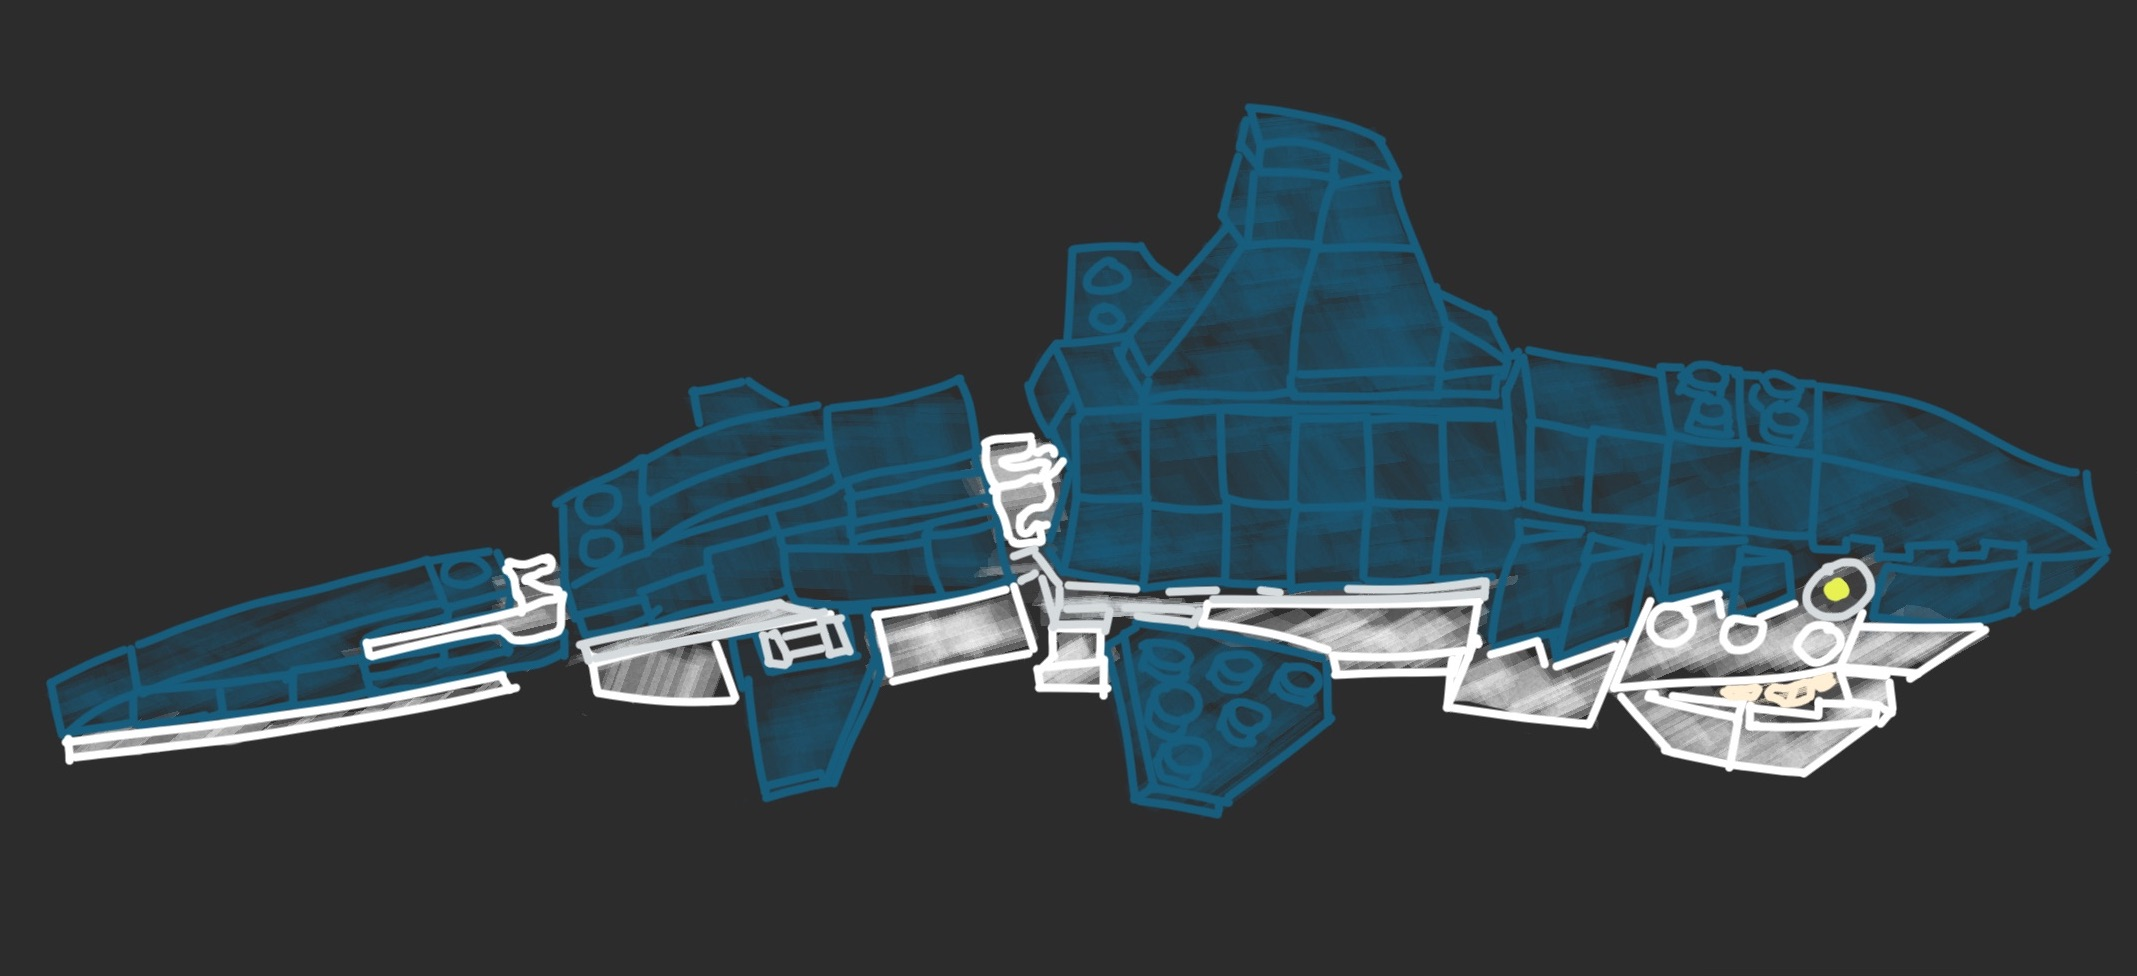
\includegraphics[width=\textwidth]{figures/legoshark} \caption[When simple tools have a common interface that allows them to be combined in different ways, like Legos, they can be combined to create complex structures, like this Lego shark]{When simple tools have a common interface that allows them to be combined in different ways, like Legos, they can be combined to create complex structures, like this Lego shark.}\label{fig:legoshark}
\end{figure}

The tools in the ``tidyverse'' operate on a similar principle. They all input one
of a few very straightforward data types, and they (almost) all output data in
the same format they input it. For most of the tools, their required format for
input and output is the ``tidy data'' format \citep{wickham2014tidy}, called a tidy
\emph{dataframe} in R---this is a dataframe that follows the rules detailed earlier
in this section.

Some of the tools require input and output of \emph{vectors} instead of tidy
dataframes \citep{wickham2014tidy}; a \emph{vector} in R is a one-dimensional string of values,
all of which are of the same data type (e.g., all numbers, or all character
strings, like names). In a tidy dataframe, each column is a vector, and the
dataframe is essentially several vectors of the same length stuck together to
make a table. Having functions that input and output vectors, then, means that
you can use those functions to make changes to the columns in a tidy dataframe.

A few functions in the ``tidyverse'' input a tidy dataframe but output data in a
different format. For example, visualizations are created using a function
called \texttt{ggplot}, as well as its helper functions and extensions. This function
inputs data in a tidy dataframe but outputs it in a type of R object called a
``ggplot object''. This object encodes the plot the code created, so in this case
the fact that the output is in a different format from the endpoint is similar
to with the ``eye'' blocks in Legos, where it's meant as a final output step, and
you don't intend to do anything further in the code once you move into that
step.

This common input / output interface, and the use of small tools that follow
this interface and can be combined in various ways, is what makes the tidyverse
tools so powerful. However, there are other good things about the tidyverse that
make it so popular. One is that it's fairly easy to learn to use the tools, in
comparison to learning how to write code for other R tools \citep{robinson2017teach, peng2018teaching}. The developers who have created the tidyverse tools have
taken a lot of effort to try to make sure that they have a clear and consistent
\emph{user interface} across tools \citep{wickham2017tidy, bryan2017data}. So far, we've
talked about the interface between functions, and how a common \emph{input / output
interface} means the functions can be chained together more easily. But there's
another interface that's important for software tools: the rules for how a
computer users employ that tool, or the \emph{user interface}.

To help understand a user interface, and how having a consistent user interface
across tools is useful, let's think about a different example---cars. When you
drive a car, you get the car to do what you want through the steering wheel, the
gas pedal, the break pedal, and different knobs and buttons on the dashboard.
When the car needs to give you feedback, it uses different gauges on the
dashboard, like the speedometer, as well as warning lights and sounds.
Collectively, these ways of interacting with your car make up the car's \emph{user
interface}. In the same way, each function in a programming language has a
collection of parameters you can set, which let you customize the way the
function runs, as well as a way of providing you output once the function has
finished running and the way to provide any messages or warnings about the
function's run. For functions, the software developer can usually choose design
elements for the function's user interface, including which parameters to
include for the function, what to name those parameters, and how to provide
feedback to the user through messages, warnings, and the final output.

If a collection of tools is similar in its user interfaces, it will make it
easier for users to learn and use any of the tools in that collection once
they've learned how to use one. For cars, this explains how the rental car
business is able to succeed. Even though different car models are very different
in many characteristics---their engines, their colors, their software---they are
very consistent in their user interfaces. Once you've learned how to drive one
car, when you get in a new car, the gas pedal, brake, and steering wheel are
almost guaranteed to be in about the same place and to operate about the same
way as in the car you learned to drive in. The exceptions are rare enough to be
memorable---think how many movies have a laughline from a character trying to
drive a car with the driver side on the right if they're used to the left or
vice versa.

The tidyverse tools are similarly designed so that they all have a very similar
user interface. For example, many of the tidyverse functions use a parameter
named ``.data'' to refer to the tidy dataframe to input into the function, and
this parameter is often the first listed for functions. Similarly, parameters
named ``.vars'' and ``.funs'' are repeatedly used over tidyverse functions, with the
same meaning in each case. What's more, the tidyverse functions are typically given names
that very clearly describe the action that the function does, like \texttt{filter},
\texttt{summarize}, \texttt{mutate}, and \texttt{group}. As a result, the final code is very clear
and can almost be ``read'' as a natural language, rather than code.

\begin{quote}
``Another part of what makes the Tidyverse effective is harder to see and,
indeed, the goal is for it to become invisible: conventions. The Tidyverse
philosophy is to rigorously (and ruthlessly) identify and obey common
conventions. This applies to the objects passed from one function to another
and to the user interface each function presents. Taken in isolation, each
instance of this seems small and unimportant. But collectively, it creates
a cohesive system: having learned one component you are more likely to be
able to guess how another different component works.'' \citep{bryan2017data}
\end{quote}

\begin{quote}
``The goal of {[}the tidy tools{]} principles is to provide a uniform interface so
that tidyverse packages work together naturally, and once you've mastered one,
you have a head start on mastering the others.'' \citep{wickhem2017tidy}
\end{quote}

As a result, the tidyverse collection of tools is pretty easy to learn, compared
to other sets of functions in scripting languages, and pretty easy to expand
your knowledge of once you know some of its functions. Several people who teach
R programming now focus on first teaching the tidyverse, given these
characteristics \citep{robinson2017teach, peng2018teaching}, and it's often a
first focus for online courses and workshops on R programming. Since it's main
data structure is the ``tidy data'' structure, it's often well worth recording
data in this format so that all these tools can easily be used to explore and
model the data.

\begin{quote}
``All our code is underpinned by the principles of tidy data, the
grammar of data manipulation, and the tidyverse R packages developed
by Wickham. This deliberate philosophy for thinking
about data helped bridge our scientific questions with the data processing
required to get there, and the readability and conciseness of
tidyverse operations makes our data analysis read more as a story
arc. Operations require less syntax---which can mean fewer potential
errors that are easier to identify---and they can be chained together,
minimizing intermediate steps and data objects that can cause clutter and
confusion. The tidyverse tools for wrangling data have
expedited our transformation as coders and made R less intimidating to
learn.'' \citep{lowndes2017our}
\end{quote}

\hypertarget{using-tidyverse-tools-with-data-in-the-tidy-data-format}{%
\subsection{Using tidyverse tools with data in the ``tidy data'' format}\label{using-tidyverse-tools-with-data-in-the-tidy-data-format}}

The tidyverse includes tools for many of the tasks you might need to
do while managing and working with experimental data. When you download
R, you get what's called \emph{base R}. This includes the main code that drives
anything you do in R, as well as functions for doing many core tasks.
However, the power of R is that, in addition to base R, you can also add
onto R through what are called \emph{packages} (sometimes also referred to
as \emph{extensions} or \emph{libraries}). These are kind of like ``booster packs''
that add on new functions for R. They can be created and contributed
by anyone, and many are collected through a few key repositories like
CRAN and Bioconductor.

All the tidyverse tools are included in R extension packages, rather than base
R, so once you download R, you'll need to download these packages as well to use
the tidyverse tools. The core tidyverse functions include functions to read in
data (the \texttt{readr} package for reading in plain text, delimited files, \texttt{readxl}
to read in data from Excel spreadsheets), clean or summarize the data (the
\texttt{dplyr} package, which includes functions to merge different datasets, make
new columns as functions of old ones, and summarize columns in the data, either
as a whole or by group), and reformat the data if needed to get it in a tidy
format (the \texttt{tidyr} package). The tidyverse also includes more precise tools,
including tools to parse dates and times (\texttt{lubridate}) and tools to work with
character strings, including using regular expressions as a powerful way to find
and use certain patterns in strings (\texttt{stringr}). Finally, the tidyverse
includes powerful functions for visualizing data, based around the \texttt{ggplot2}
package, which implements a ``grammar of graphics'' within R.

You can install and load any of these tidyverse packages one-by-one using the
\texttt{install.packages} and \texttt{library} functions with the package name from within R.
If you are planning on using many of the tidyverse packages, you can also
install and load many of the tidyverse functions by installing a package called
``tidyverse'', which serves as an umbrella for many of the tidyverse packages.

In addition to the original tools in the tidyverse, many people have developed
\emph{tidyverse} extensions---R packages that build off the tools and principles in
the tidyverse. These often bring the tidyverse conventions into tools for
specific areas of science. For example, the \texttt{tidytext} package provides tools to
analyze large datasets of text, including books or collections of tweets, using
the tidy data format and tidyverse-style tools. Similar tidyverse extensions
exist for working with network data (\texttt{tidygraph}) or geospatial data (\texttt{sf}).
Extensions also exist for the visualization branch of the tidyverse
specifically. These include \emph{ggplot extensions} that allow users to create
things like calendar plots (\texttt{sugrrants}), gene arrow maps (\texttt{gggene}), network
plots (\texttt{igraph}), phytogenetic trees (\texttt{ggtree}) and anatogram images
(\texttt{gganatogram}). These extensions all allow users to work with data that's in a
``tidy data'' format, and they all provide similar user interfaces, making it
easier to learn a large set of tools to do a range of data analysis and
visualization, compared to if the set of tools lacked this coherence.

\hypertarget{practice-quiz}{%
\subsection{Practice quiz}\label{practice-quiz}}

\hypertarget{module4}{%
\section{Designing templates for ``tidy'' data collection}\label{module4}}

This module will move from the principles of the ``tidy'' data format to the
practical details of designing a ``tidy'' data format to use when collecting
experimental data. We will describe common issues that prevent biomedical
research datasets from being ``tidy'' and show how these issues can be avoided. We
will also provide rubrics and a checklist to help determine if a data collection
template complies with a ``tidy'' format.

\textbf{Objectives.} After this module, the trainee will be able to:

\begin{itemize}
\tightlist
\item
  Identify characteristics that keep a dataset from being ``tidy''
\item
  Convert data from an ``untidy'' to a ``tidy'' format
\end{itemize}

In this module, we will use a real example of data collected in a biomedical laboratory.
We'll use this example to show how data is often collected in a way that is
not ``tidy'', focusing on the features of data collection that make it ``untidy''.
We'll then describe some general principles for why and how to instead create and
use tidy (or at least tidier) templates to collect data in the laboratory, and
show how this can be the first step in a pipeline to creating useful, attractive,
and reproducible reports that describe the data you collected. This module will
focus on the principles of templates for tidy data collection, while in the next
module we'll dig deeper into the details of making this conversion for the
example dataset that we use as a demonstration in this module.

\hypertarget{exampledata-on-rate-of-bacterial-growth}{%
\subsection{Example---Data on rate of bacterial growth}\label{exampledata-on-rate-of-bacterial-growth}}

Throughout this module, we'll use a real dataset to illustrate principles of
data collection in a biomedical laboratory. First, let's start by looking at the
original data collection template, and use this to walk through some details of
this dataset.

Figure \ref{fig:growthexcel1} provides an annotated view of the data set, showing
the format used when the data were originally collected:

\begin{figure*}
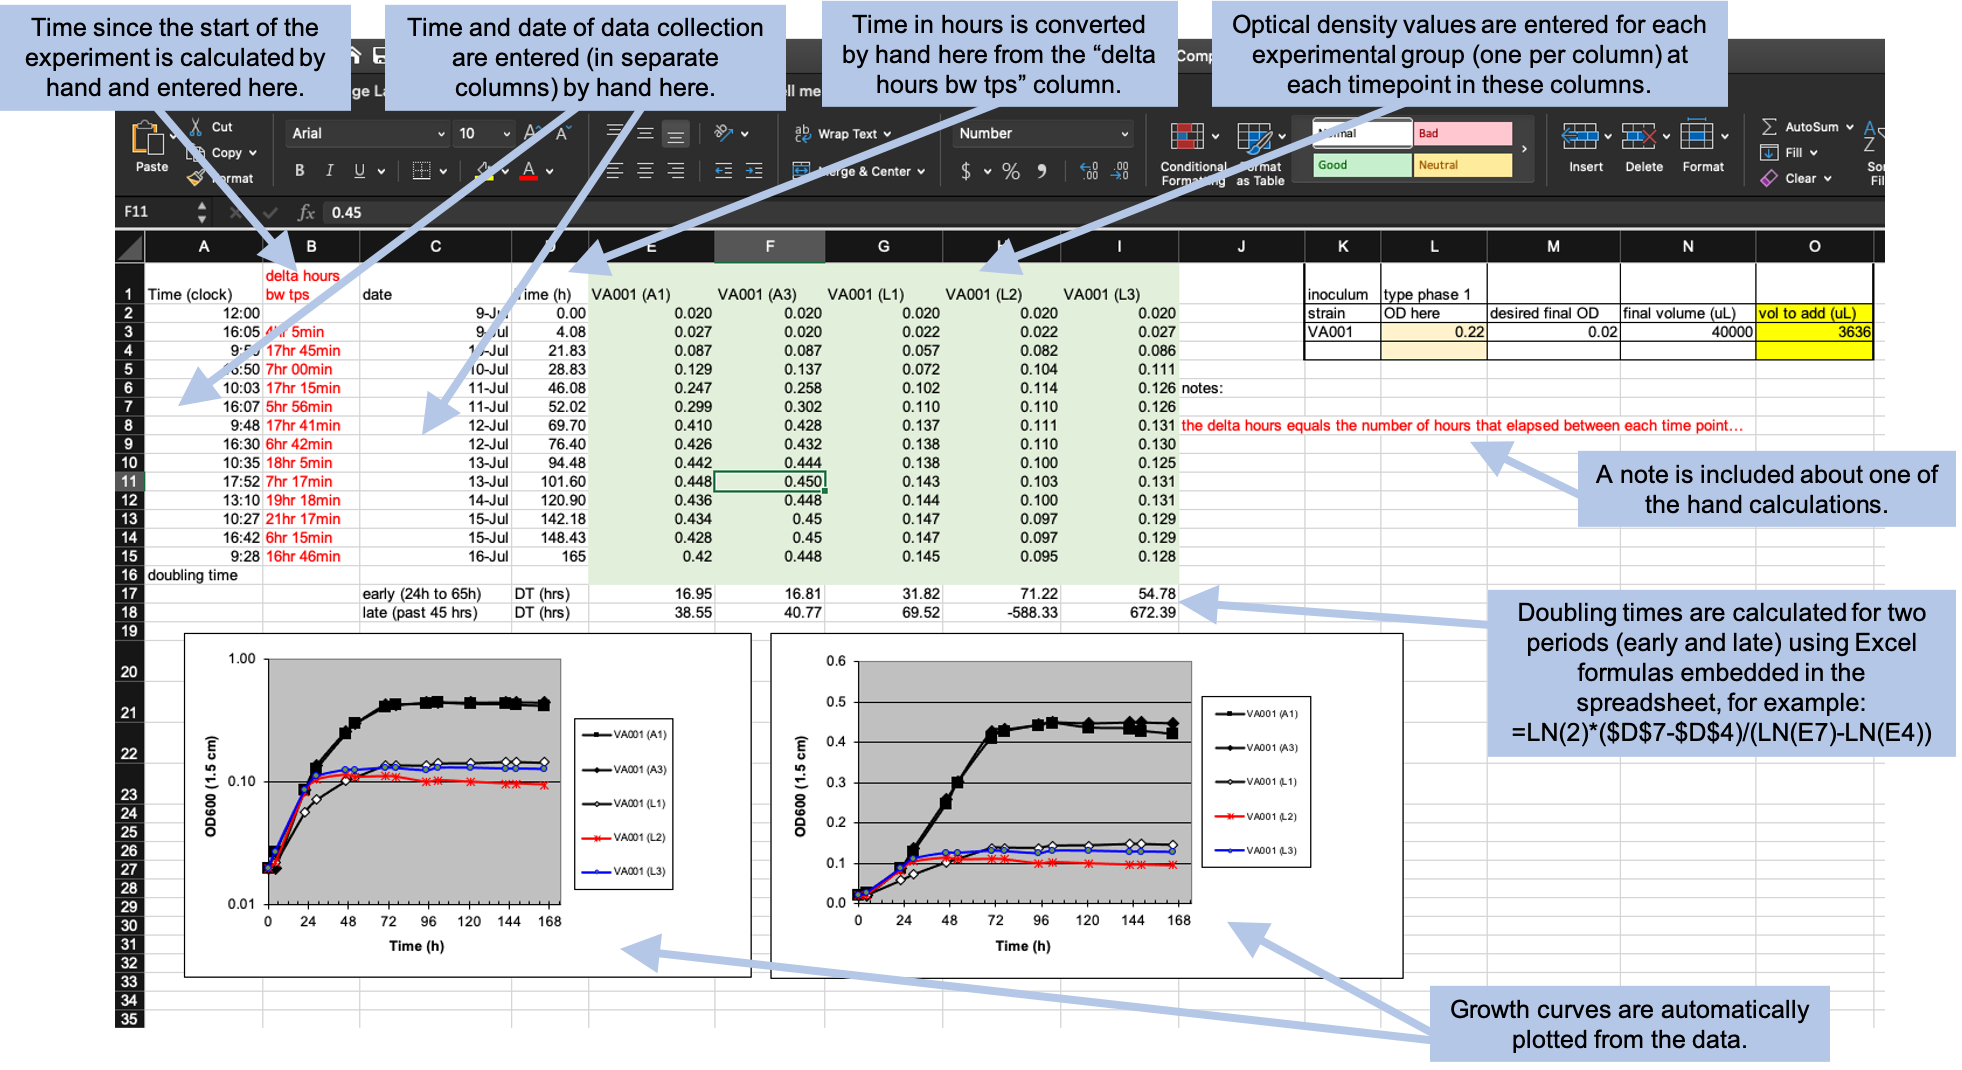
\includegraphics[width=\textwidth]{figures/growth_curve_example} \caption[Example of an Excel spreadsheet used to record and analyze data for a laboratory experiment]{Example of an Excel spreadsheet used to record and analyze data for a laboratory experiment. Annotations highlight where data is entered by hand, where calculations are done by hand, and where embedded Excel formulas are used. The figures are created automatically using values in a specified column.}\label{fig:growthexcel1}
\end{figure*}

These data were collected to measure the compare growth yield and doubling time
of \emph{Mycobacterium tuberculosis} (the bacteria that causes tuberculosis in
humans) under two conditions---high oxygen and low oxygen. In humans, M.
tuberculosis can persist for years or decades in granulomas, and the centers of
these granulomas are often hypoxic (low in oxygen). Therefore, it's important to
understand how these bacteria grow in hypoxic conditions.

To conduct this experiment, the researchers used test tubes that were capped
with sealed caps to prevent and air exchange between the contents of the tube
and the environment. Inside the tubes, the amount of oxygen was controlled
by shifting the ratio of the volume of the culture (the liquid with nutrients
in which the M. tuberculosis will grow) versus the volume of air.
In the high oxygen condition, a lower volume of culture was used, which leaves
room for a lot of air in the top of the tube. In the low oxygen condition,
the tube was filled almost to the top with culture, which left very little air
at the top of the tube.

Once the tubes were filled and capped, they were left to grow for about a week.
During this time, the researchers took several measurements to determine the
growth of the bacteria in each tube. To do this, they used a spectrophotometer
to track increases in optical density (absorbance at 600 nm) over time. This
method gives a measurement of turbidity in each tube that is directly proportional
to the cell mass in the tube, and so provides a measure of how much the
bacteria has grown since the start of the experiment.

To record data from this experiment, researchers used the spreadsheet shown in
Figure \ref{fig:growthexcel1}. This spreadsheet is an example of a data
collection template---it was created not only for this experiment, but also for
other experiments that this research group conducts to measure bacterial growth
under different conditions. It was designed to allow a researcher working in the
laboratory to record measurements over the course of the experiment. This
specific spreadsheet allowed the researcher who was conducting the experiment to
(1) calculate the amount of initial inoculum (cell culture) to add to each tube
to begin the study, (2) record the raw data absorbance measurements, (3) graph
the data on both a log and linear scale, and (4) calculate doubling time in two
phases of growth using the equation listed above.

Let's take a closer look at some of the features of this spreadsheet. First, it
has a section on the top right that focuses on data collection during the
experiment, with one row for each time when the tubes were measured for the cell
mass within the tube. This section of the spreadsheet starts with several
columns related to the time of each measurement, including the clock time at
measurement (column A), the difference in time (hours) between each time point
in which data were collected (column B), the date on which data were gathered
(column C), and the time in hours for each data point from the start of the
study for graphing purposes (column D). The columns for clock time (A) and date
(C) were recorded by hand, while the columns for time since the start of the
experiment (B and D) were calculated or converted by hand from these values and
then entered in the column. The remaining columns (E--I) provide data on the
optical density (absorbance at 600 nm), which is directly proportional to cell
mass in the tube. There is one column per test tub, and each of these column
labels includes a test tube ID (A1, A3, L1, L2, L3). If a tube ID starts with
``A'', it was grown in high oxygen conditions, and if it starts with ``L'', it was
grown in low oxygen conditions.

Next, the spreadsheet has areas that provide summaries of the data, calculated
using embedded formulas or through the spreadsheet's plotting functions. For
example, rows 17--18 provide calculations of the doubling time of the bacteria
in each tube for two periods (early and late in the experiment), while two
growth curves are plotted at the bottom of the spreadsheet.

Finally, the spreadsheet includes a couple of other features, including some
written notes about one of the hand calculations and a macro in the top right
that can be used by the researcher to calculate the amount of the initial
inoculum to add to each tube at the start of the experiment.

What the researchers found appealing about the format of this spreadsheet was
the ease with which the research collecting data in the laboratory could
accomplish the study goals. They also cited transparency of the raw data and
ease with which additional sampling data points could be added. The data being
graphed in real time, and the inclusion of a simple macro to calculate doubling
time, allowed the research in the laboratory to see tangible differences between
the two assay conditions as data were collected over the one-week experiment.
However, many of these features can have undesired consequences. They can increase
the chance of errors in recording the data and in calculating summaries based on the
data. They also make it hard to move the data into a reproducible pipeline, and
so limit opportunities for more sophisticated analysis and visualization. In the
next section of this module, we'll highlight features of data collection templates
like this one that can make data collection ``untidy''. In the section after that,
we'll discuss how you could create a new data collection template for this example
data that would be tidier, and use this to open a more general discussion of
principles of ``tidy'' data collection templates.

\hypertarget{features-that-make-data-collection-templates-untidy}{%
\subsection{Features that make data collection templates ``untidy''}\label{features-that-make-data-collection-templates-untidy}}

There are several features of the data collection template shown in Figure
\ref{fig:growthexcel1} that make it ``untidy'', in the sense of making it
difficult to integrate the collected data in a data analysis pipeline that
includes reading the data into a statistical program like R, Perl, or Python to
conduct data analysis and visualization. There are also features that make it
prone to errors in data collection and analysis.

First, these data will be hard to read into a statistical program from this
spreadsheet because the raw data (the time points each observation was collected
and the optical density for the sample at that time point) form only part of the
spreadsheet (Figure \ref{fig:extractraw}). The ``extra'' elements on the
spreadsheet, which include the output from calculations, plots, macros, and
notes, make it harder to isolate the raw data from the file when using a
statistical program.

\begin{figure*}
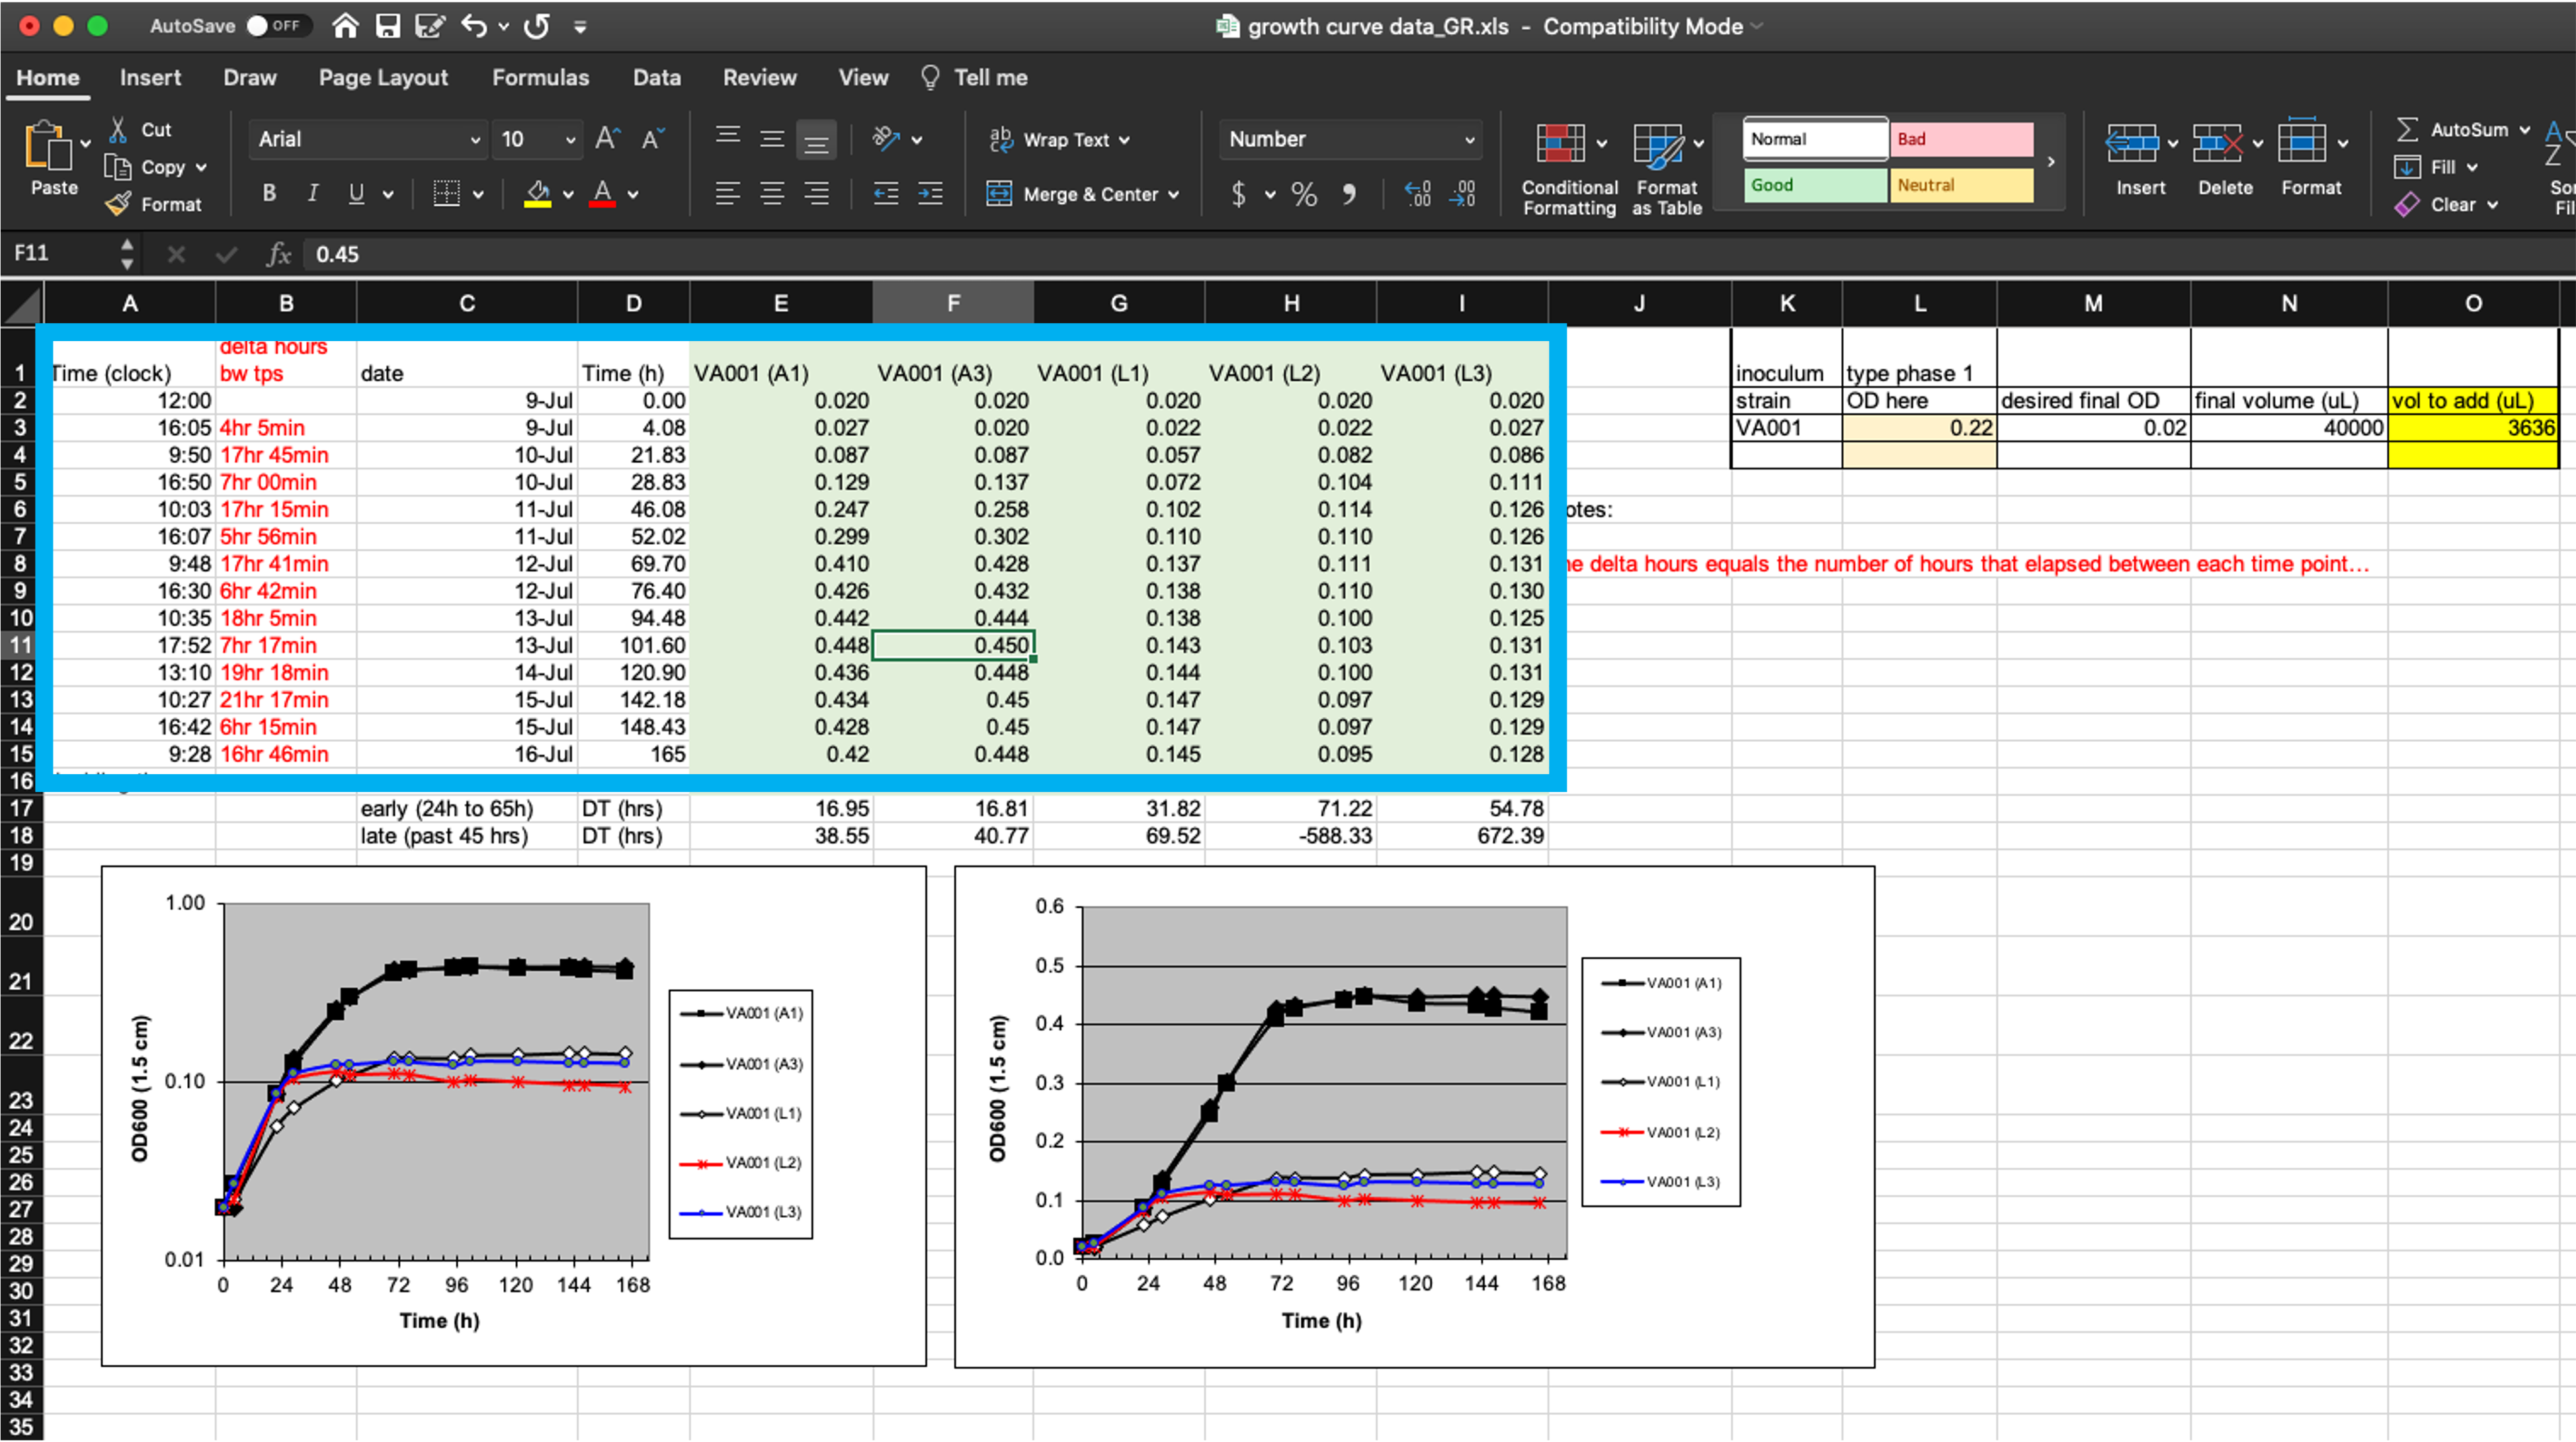
\includegraphics[width=\textwidth]{figures/growth_curve_raw_data} \caption[Isolating raw data collected in a template from extra elements]{Isolating raw data collected in a template from extra elements. The box in this figure highlights the area of the spreadsheet where data are collected. All other elements of the spreadsheet focus on other aims (e.g., summarizing these data, adding notes, macros for experimental design). Those other elements make it difficult to extract the raw data for more advanced analysis and visualization through a statistical program like R, Python, or Perl.}\label{fig:extractraw}
\end{figure*}

While these extra elements make it hard to extract the raw data, it isn't
impossible. Programming languages like R include functions to read data in from
a spreadsheet, and these functions often provide options to specify the sheet of
the file to read in, as well as the rows and columns to read from a specific
sheet. In the example spreadsheet in Figure \ref{fig:extractraw}, for example,
you could specify to read in only rows 1--15 of columns A--I, to focus on the
raw data. However, one goal of reproducible research is to create tools and
pipelines that are robust---that is, ones that still work as desired when the
raw data is changed in small ways, or even across different raw data files. In
later modules, in fact, we'll look at how we can use these principles to create
tools that can be applied consistently across multiple studies to make data
analysis of laboratory data both more efficient and reproducible. Therefore,
while we could customize code to read in data from a specific part of a complex
spreadsheet, like that shown in Figure \ref{fig:extractraw}, this customization
would make the code less robust. If we asked the statistical program to read in
rows 1--15 of columns A--I, for example, the code would perform incorrectly if
we later added one more time point to the experiment, or if we tried to use the
same template for an experiment that used more test tubes. If we instead use a
template that only records the raw data, without additional elements, then we
can create more robust tools, since we can write code to read in whatever is in
a spreadsheet, rather than restricting to certain rows and columns. Any analysis,
summaries, or visualizations that we'd like to perform on the raw data can be
done through reproducible reports---which we'll show an example of later for
this example data---rather than directly in a spreadsheet.

Next, the example template helps demonstrate how specific ways of recording data
can make the template less tidy. First, let's look at how the template records
the time of each measurement. It does this using four separate columns
(Figure \ref{fig:extractraw}). In column C, the researcher records the date a
measurement was taken, and in Column A he or she records the clock time of the
measurement. The experiment was started, for example, at 12:00 PM (``12:00'' in column A)
on July 9 (``9-Jul'' in column C). These values are entered by hand by the researcher.
Next, these values are used to calculate, for each measurement, how long it had been
since the start of the experiment. This value is recorded in two separate ways---as
hours and minutes in column B and converted into hours and percents of hours (using
decimals) in column D. For example, the second measurement was taken at 4:05 PM
on July 9 (``16:05'' in column A and ``9-Jul'' in column C), which is 4 hours and 5 minutes
after the start of the experiment (``4hr 5min'' in column B) or, since 5 minutes is about
8\% of an hour, 4.08 hours after the start of the experiment (``4.08'' in column D).

\begin{figure}
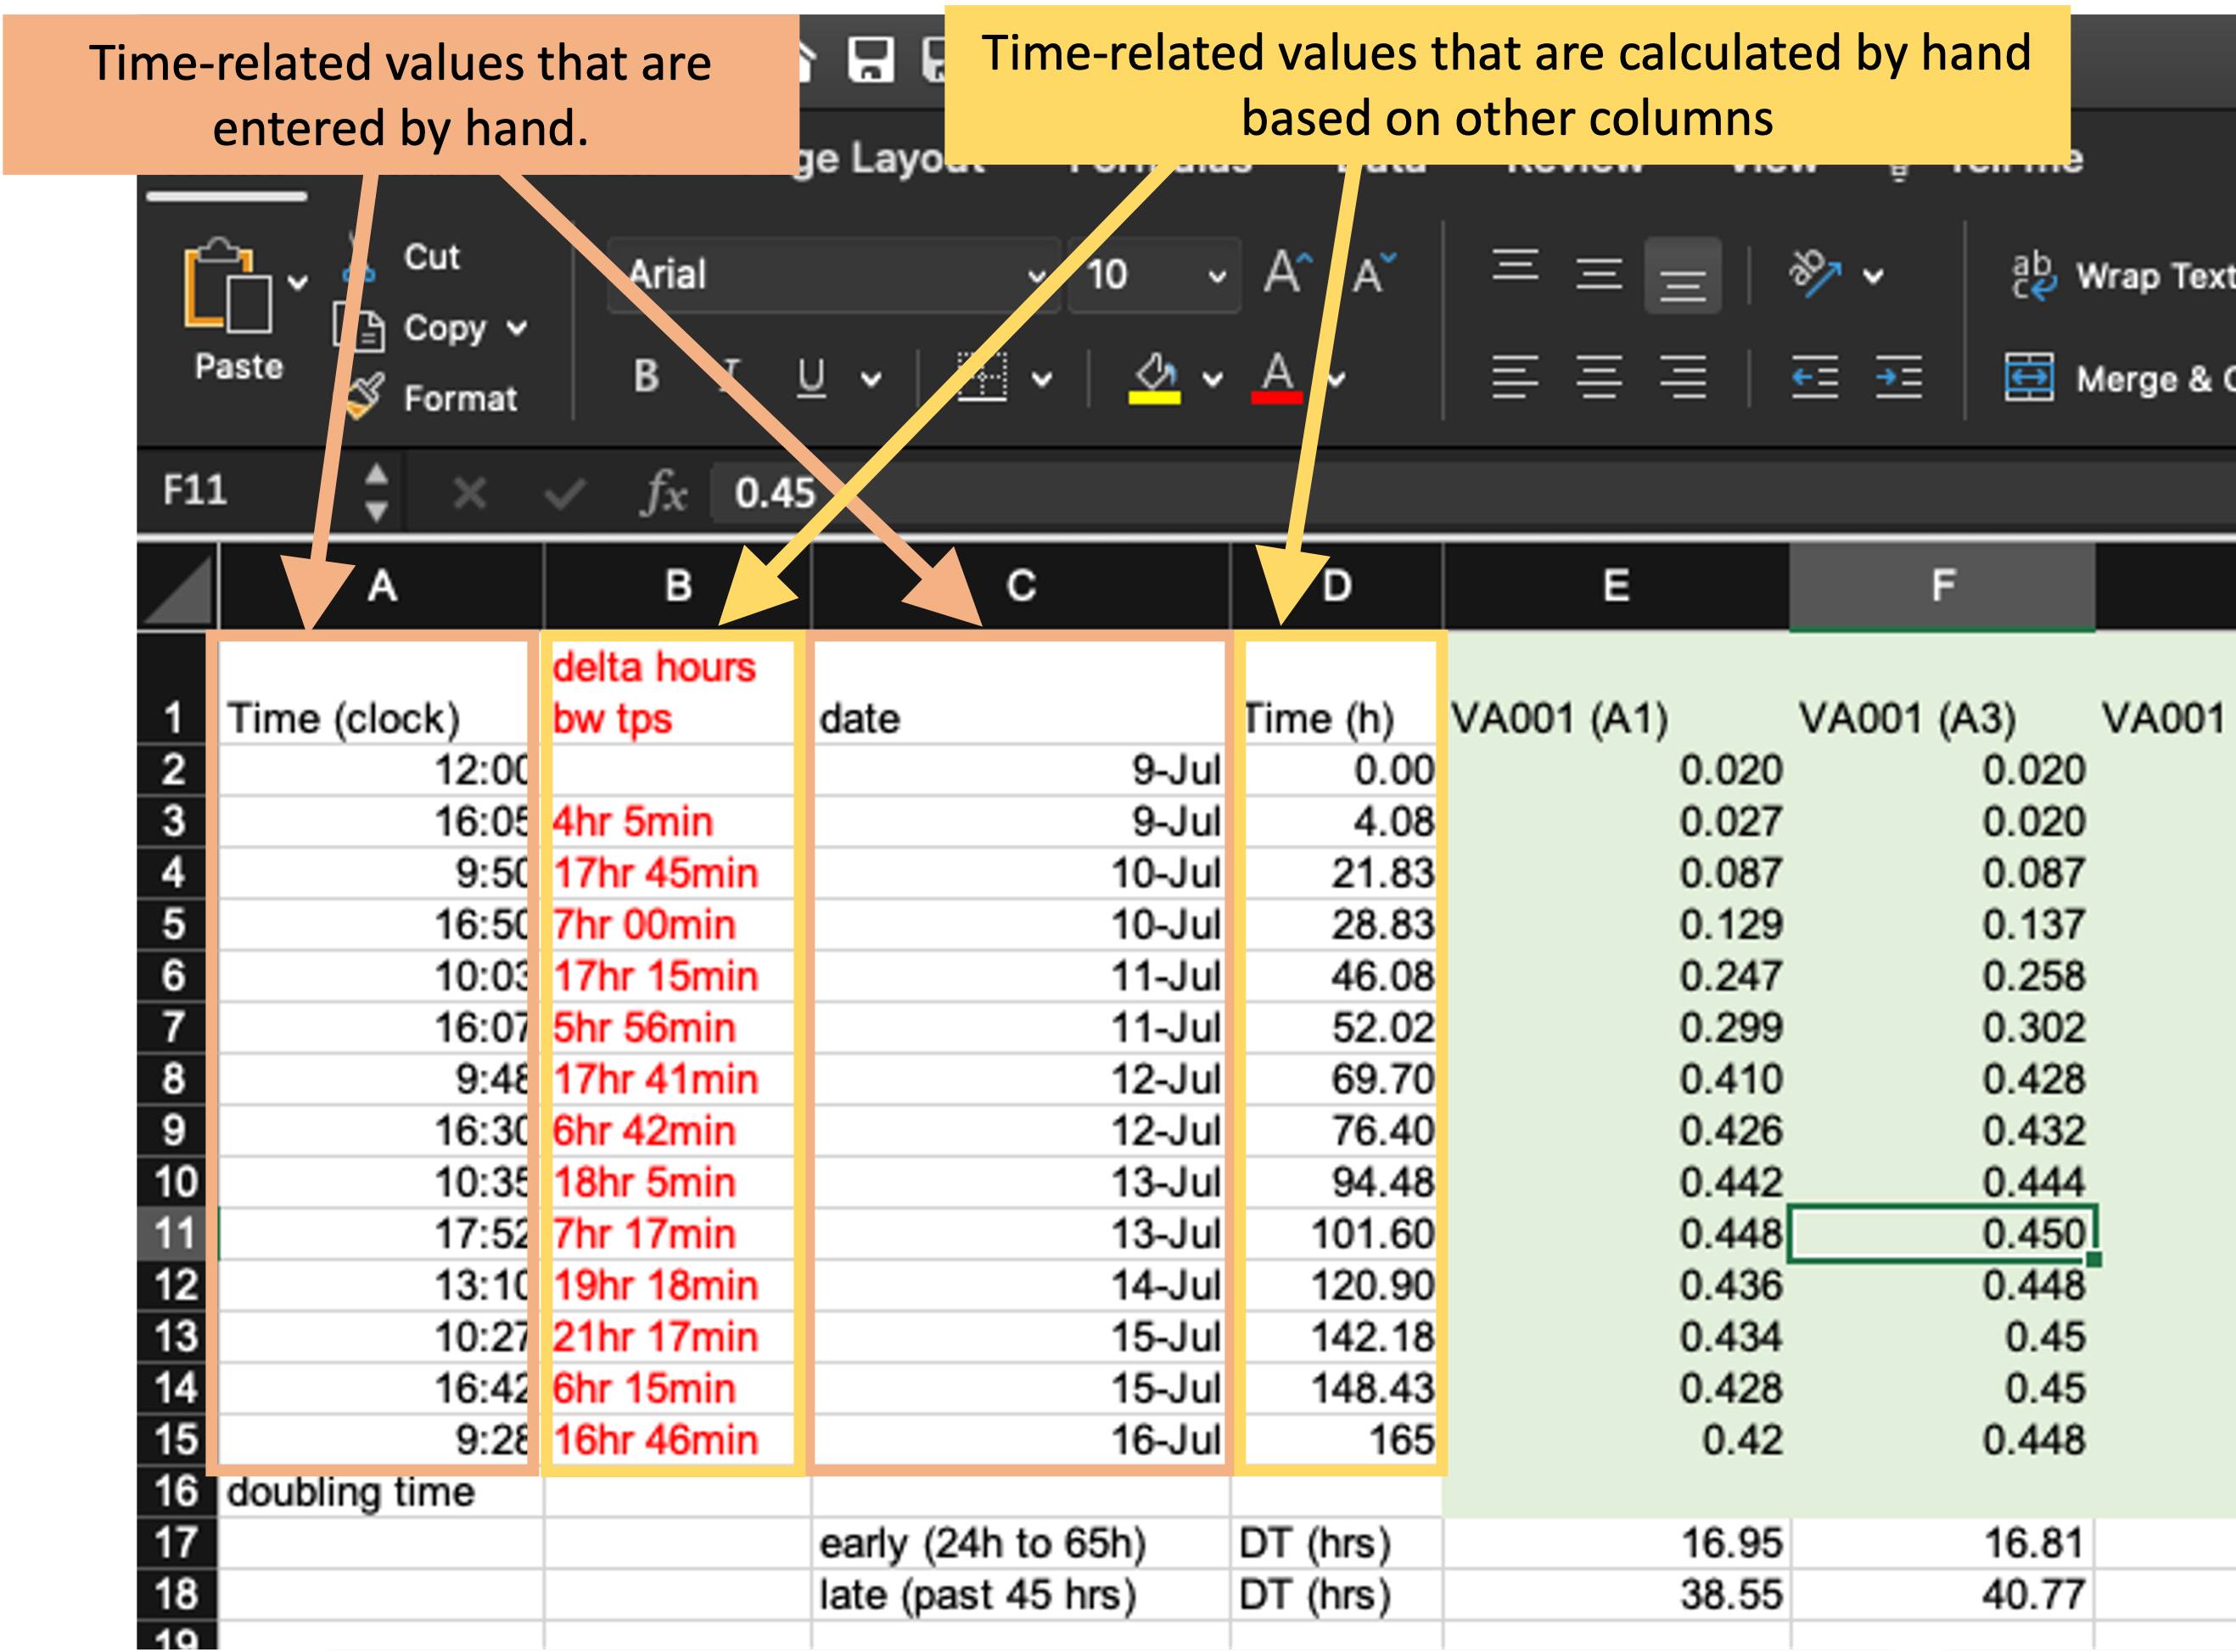
\includegraphics[width=\textwidth]{figures/growth_curve_time_measures} \caption[Measurements of time in the example data collection template]{Measurements of time in the example data collection template. The four highlighted columns (columns A, B, C, and D) are all used in this spreadsheet to record time. The methods of recording time in this template, however, may make it more likely to create errors in data recording and collection and will make it harder to use the data in a reproducible pipeline.}\label{fig:timemeasures}
\end{figure}

There are a few things that could be changed about how the time data are
recorded here that could make this data collection template tidier. First, it
would be better to focus only on recording the raw data, rather than adding
calculations based on that data. Columns B and D in Figure \ref{fig:extractraw}
are both the output from calculations. Anytime a spreadsheet includes a
calculation, it creates the room for mistakes in data collection and analysis.
Often, calculations in a spreadsheet will be done using embedded formulas. These
can cause problems anytime new columns or rows are added to the data, as that
can shift the cells meant to be used in the calculation. Further, these formulas
are embedded in the spreadsheet, where they can't be seen and checked very
easily, which makes it easy to miss a typo or other error in the formula. In the
example in Figure \ref{fig:extractraw}, columns B and D aren't calculated by
embedded formulas, but rather calculated by the researcher by hand and then
entered. This can create the room for user error with each calculation and each
data entry. Later, we'll see how we can ``tidy'' this data collection template by
removing columns that calculate time (columns B and D) and instead doing that
calculation once the raw data are read into a statistical program.

The second thing that could be changed is how the template records the date and time
of the measurement. Currently, it uses two columns (A and C) to record this information.
However, each piece of information is useless without the other---instead, they must
be known jointly to do things like calculate the time since the start of the
experiment. It would therefore be tidier to record this information in a single column.
For example, instead of recording the starting time of the experiment as ``12:00'' in
column A and ``9-Jul'' in column C, you could record it as ``July 9, 2019 12:00'' in a
single date-time column. In this example, adding the year (``2019'') to the date will
also make this data point easier to work with in a programming language, as these often
have special functions to work with data in date-time classes, but all elements of the
date and/or time must be included to convert data points into these useful classes.

Next, let's look at how the template collects data related to cell growth in each tube
(columns E--I, Figure \ref{fig:growthmeasures}).

\begin{figure*}
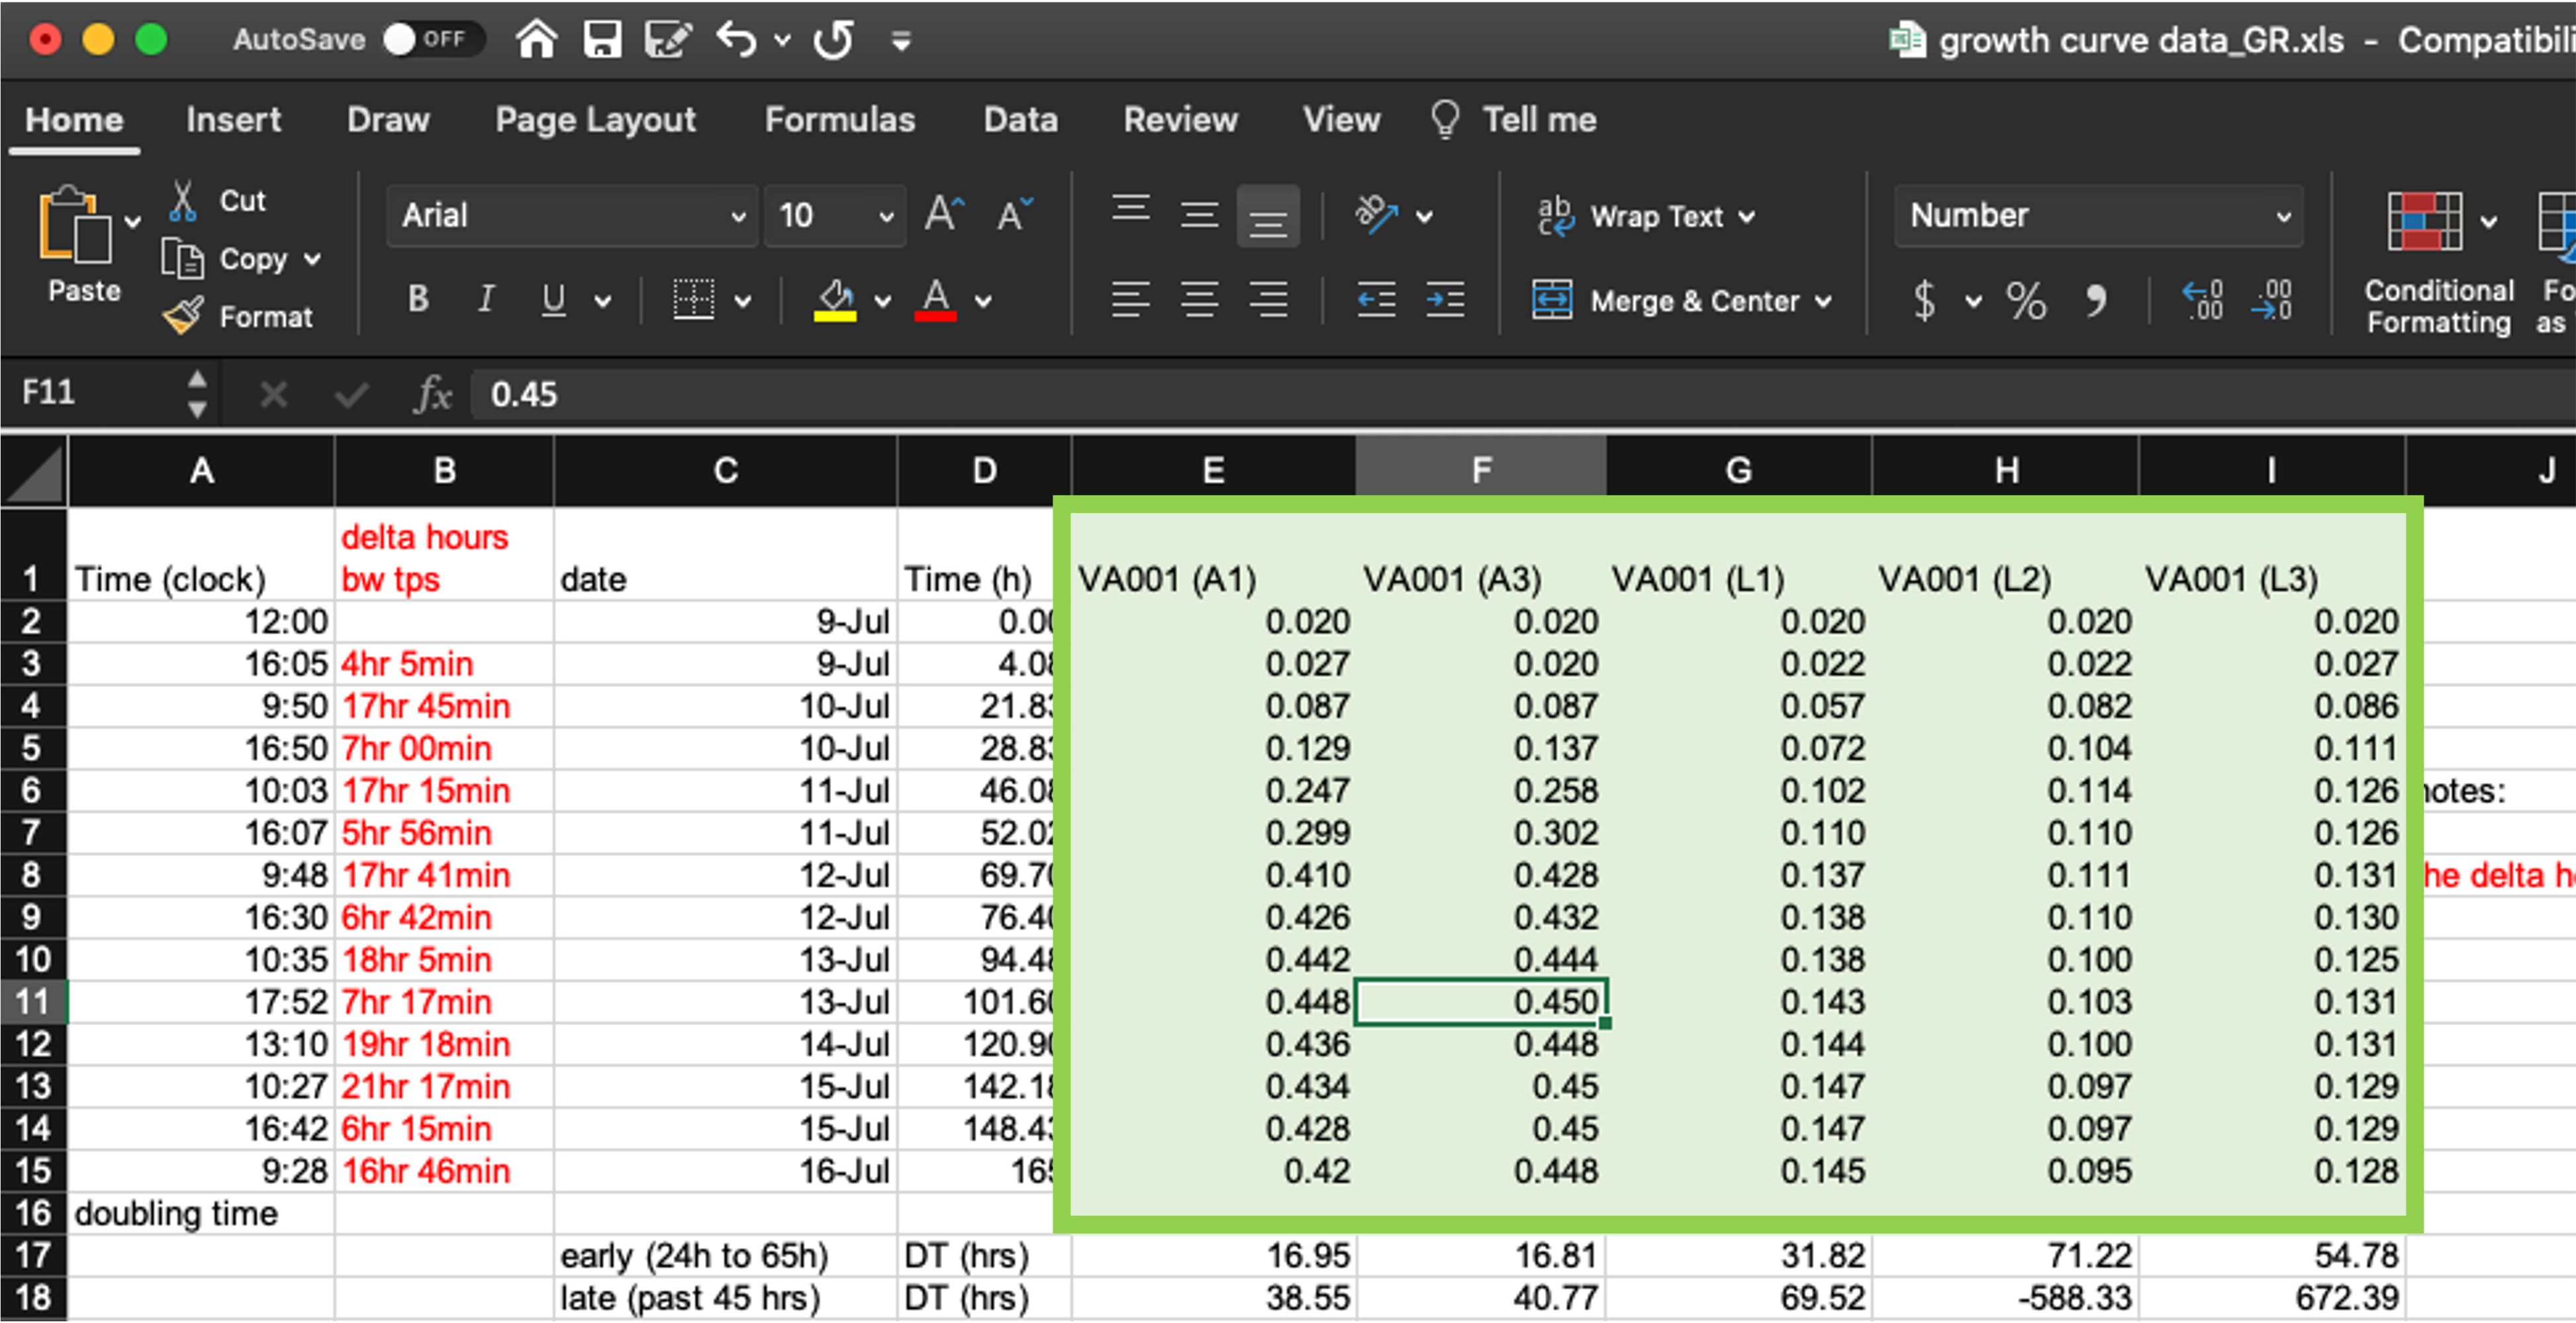
\includegraphics[width=\textwidth]{figures/growth_curve_growth_measures} \caption[Measurements of bacterial growth in the example data collection template]{Measurements of bacterial growth in the example data collection template. The five highlighted columns (columns E--I) are all used in this spreadsheet to record optical density in each test tube at each measurement time.}\label{fig:growthmeasures}
\end{figure*}

These data are recorded in a format that will work pretty well. Strictly speaking, they
aren't full ``tidy'', since the column headers include information that we might want to
use as variables in analysis and visualization. Specifically, each test tube's ID is
incorporated in the column name where measurements for that tube are recorded, since
each test tube is recorded using a separate column. If we want to run analysis where we
estimate values for each test tube, or create plots where each test tube's measurements
are shown with a separate line, then we'll need to convert the format of the data a bit.
However, that's quite easy to do in more statistical programming languages now, and so it's
reasonable to compromise on this element of ``tidiness'' in the data. As we'll show in the
next module, changing this layout in the original data collection would require the researcher
to re-type the measurement date and time several times and would result in the spreadsheet
being longer, and so harder to see at once when recording data. We'll discuss this balance
in designing data collection templates more in the next module, when we create a tidier version
of this example data collection template.

There is a final element we'd like to highlight on this example template that could make the
data hard to integrate into a reproducible pipeline. {[}Column names, other areas where special
characters, formatting, etc. may cause issues.{]} \ldots{} Figure \ref{fig:growthformatting}.

\begin{figure*}
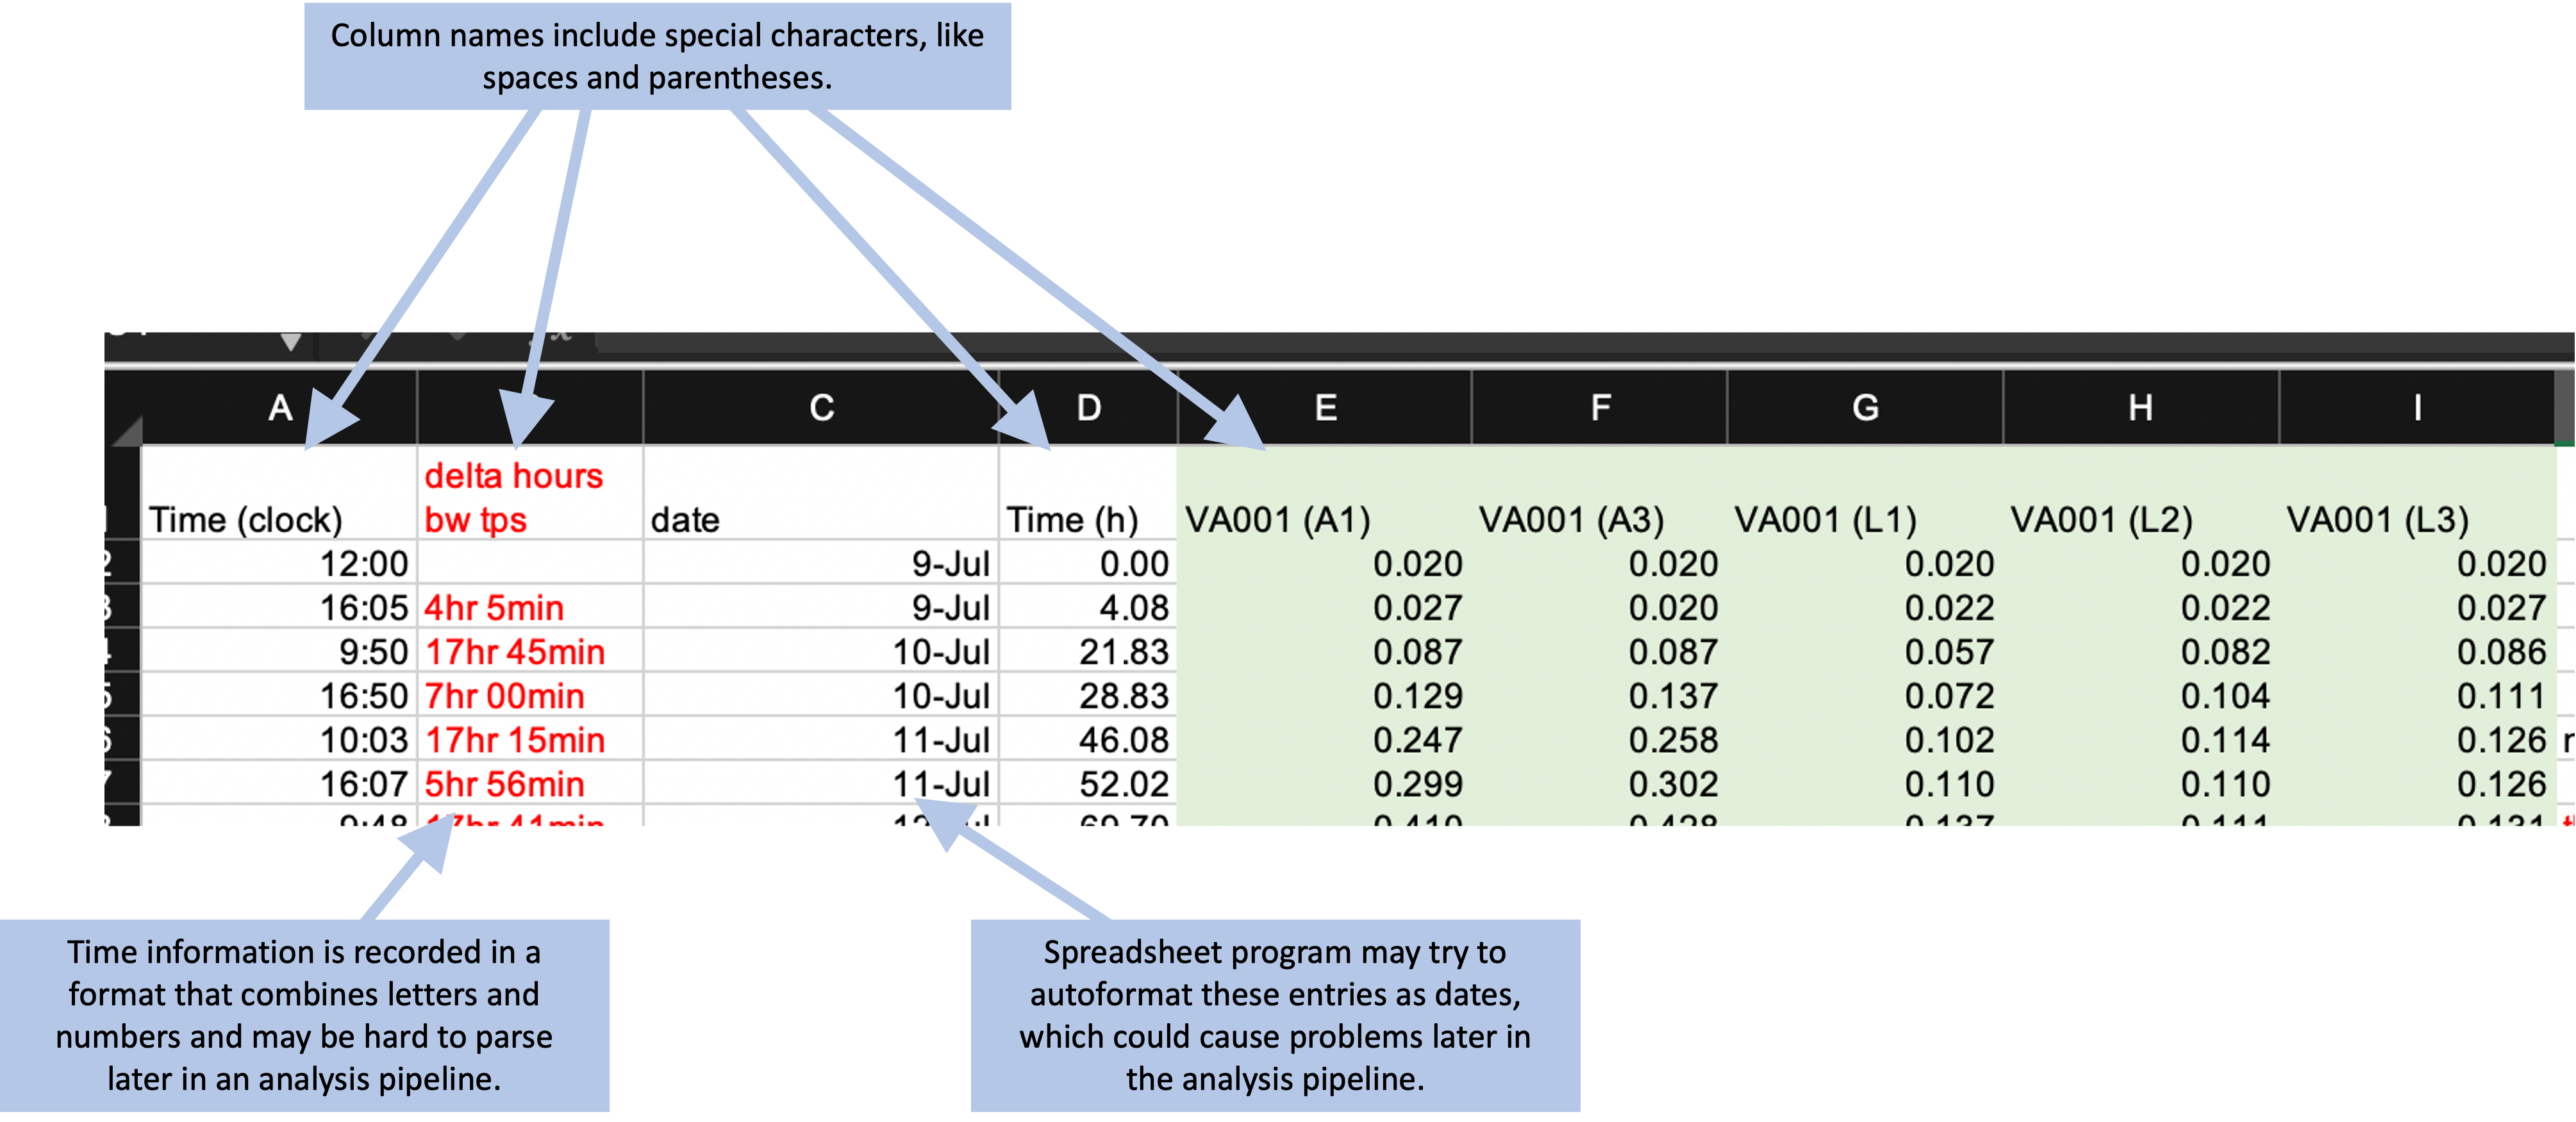
\includegraphics[width=\textwidth]{figures/growth_curve_formatting} \caption[Examples of special characters and formatting in the example template that could cause problems later in a data analysis pipeline]{Examples of special characters and formatting in the example template that could cause problems later in a data analysis pipeline.}\label{fig:growthformatting}
\end{figure*}

\hypertarget{converting-to-a-tidier-format-for-data-collection-templates}{%
\subsection{Converting to a ``tidier'' format for data collection templates}\label{converting-to-a-tidier-format-for-data-collection-templates}}

Now that we've looked at characteristics that can make a data collection template ``untidy'', let's
go through some principles for creating ``tidy'' templates to record the same data. There are three
basic principles for designing ``tidy'' templates that will go a long way to creating ways to
collect data in a research group that can be easily used within a reproducible analysis pipeline.
These three principles are:

\begin{enumerate}
\def\labelenumi{\arabic{enumi}.}
\tightlist
\item
  Limit the template to the collection of data.
\item
  Make sensible choices when dividing data collection into rows and columns.
\item
  Avoid characters or formatting that will make it hard for a computer program to process the data.
\end{enumerate}

The first principle in designing a tidier template for collecting laboratory data is to \textbf{limit the
template to the collection of data}. The key here is the word ``collection''. A tidy template will
avoid any calculations done on the original data and instead focus only on the initial data that
the researcher records for the experiment.

\ldots{} {[}Includes all macros, plots, summaries, notes. Could also include embedded formulas or columns based
on hand calculations.
Could also include formatting that's meant to contain info about the data---things like color
to show one experimental condition or the other.{]} \ldots{}

The second principle is to \textbf{make sensible choices when dividing data collection into rows and columns}.
There are many different ways that you could spread the data collection into rows and columns.
\ldots{}

The third principle is to \textbf{avoid characters or formatting that will make it
hard for a computer program to process the data}.

{[}Special characters. Spaces. Really long column names. Dates in Excel{]}

These three principles are an excellent starting point for designing a ``tidy'' template for collecting
data, and they often
{[}Others: Use things like column names to include information (starts with ``A''---one treatment; starts
with ``B''---a different one){]}

When you convert data collection templates to ``tidier'' formats, they will
typically look much simpler than the templates that your research group may have
been using. In the example experiment that we described earlier in this module,
this process of tidying the template results in a template like that shown in
Figure \ref{fig:growthexcel1} (in the next module, we'll walk through all the
steps to create this tidier template, using this principles we've covered in
this module). By comparison, the starting template for data collection for this
experiment is shown in Figure \ref{fig:growthexcel1}.

\begin{figure}
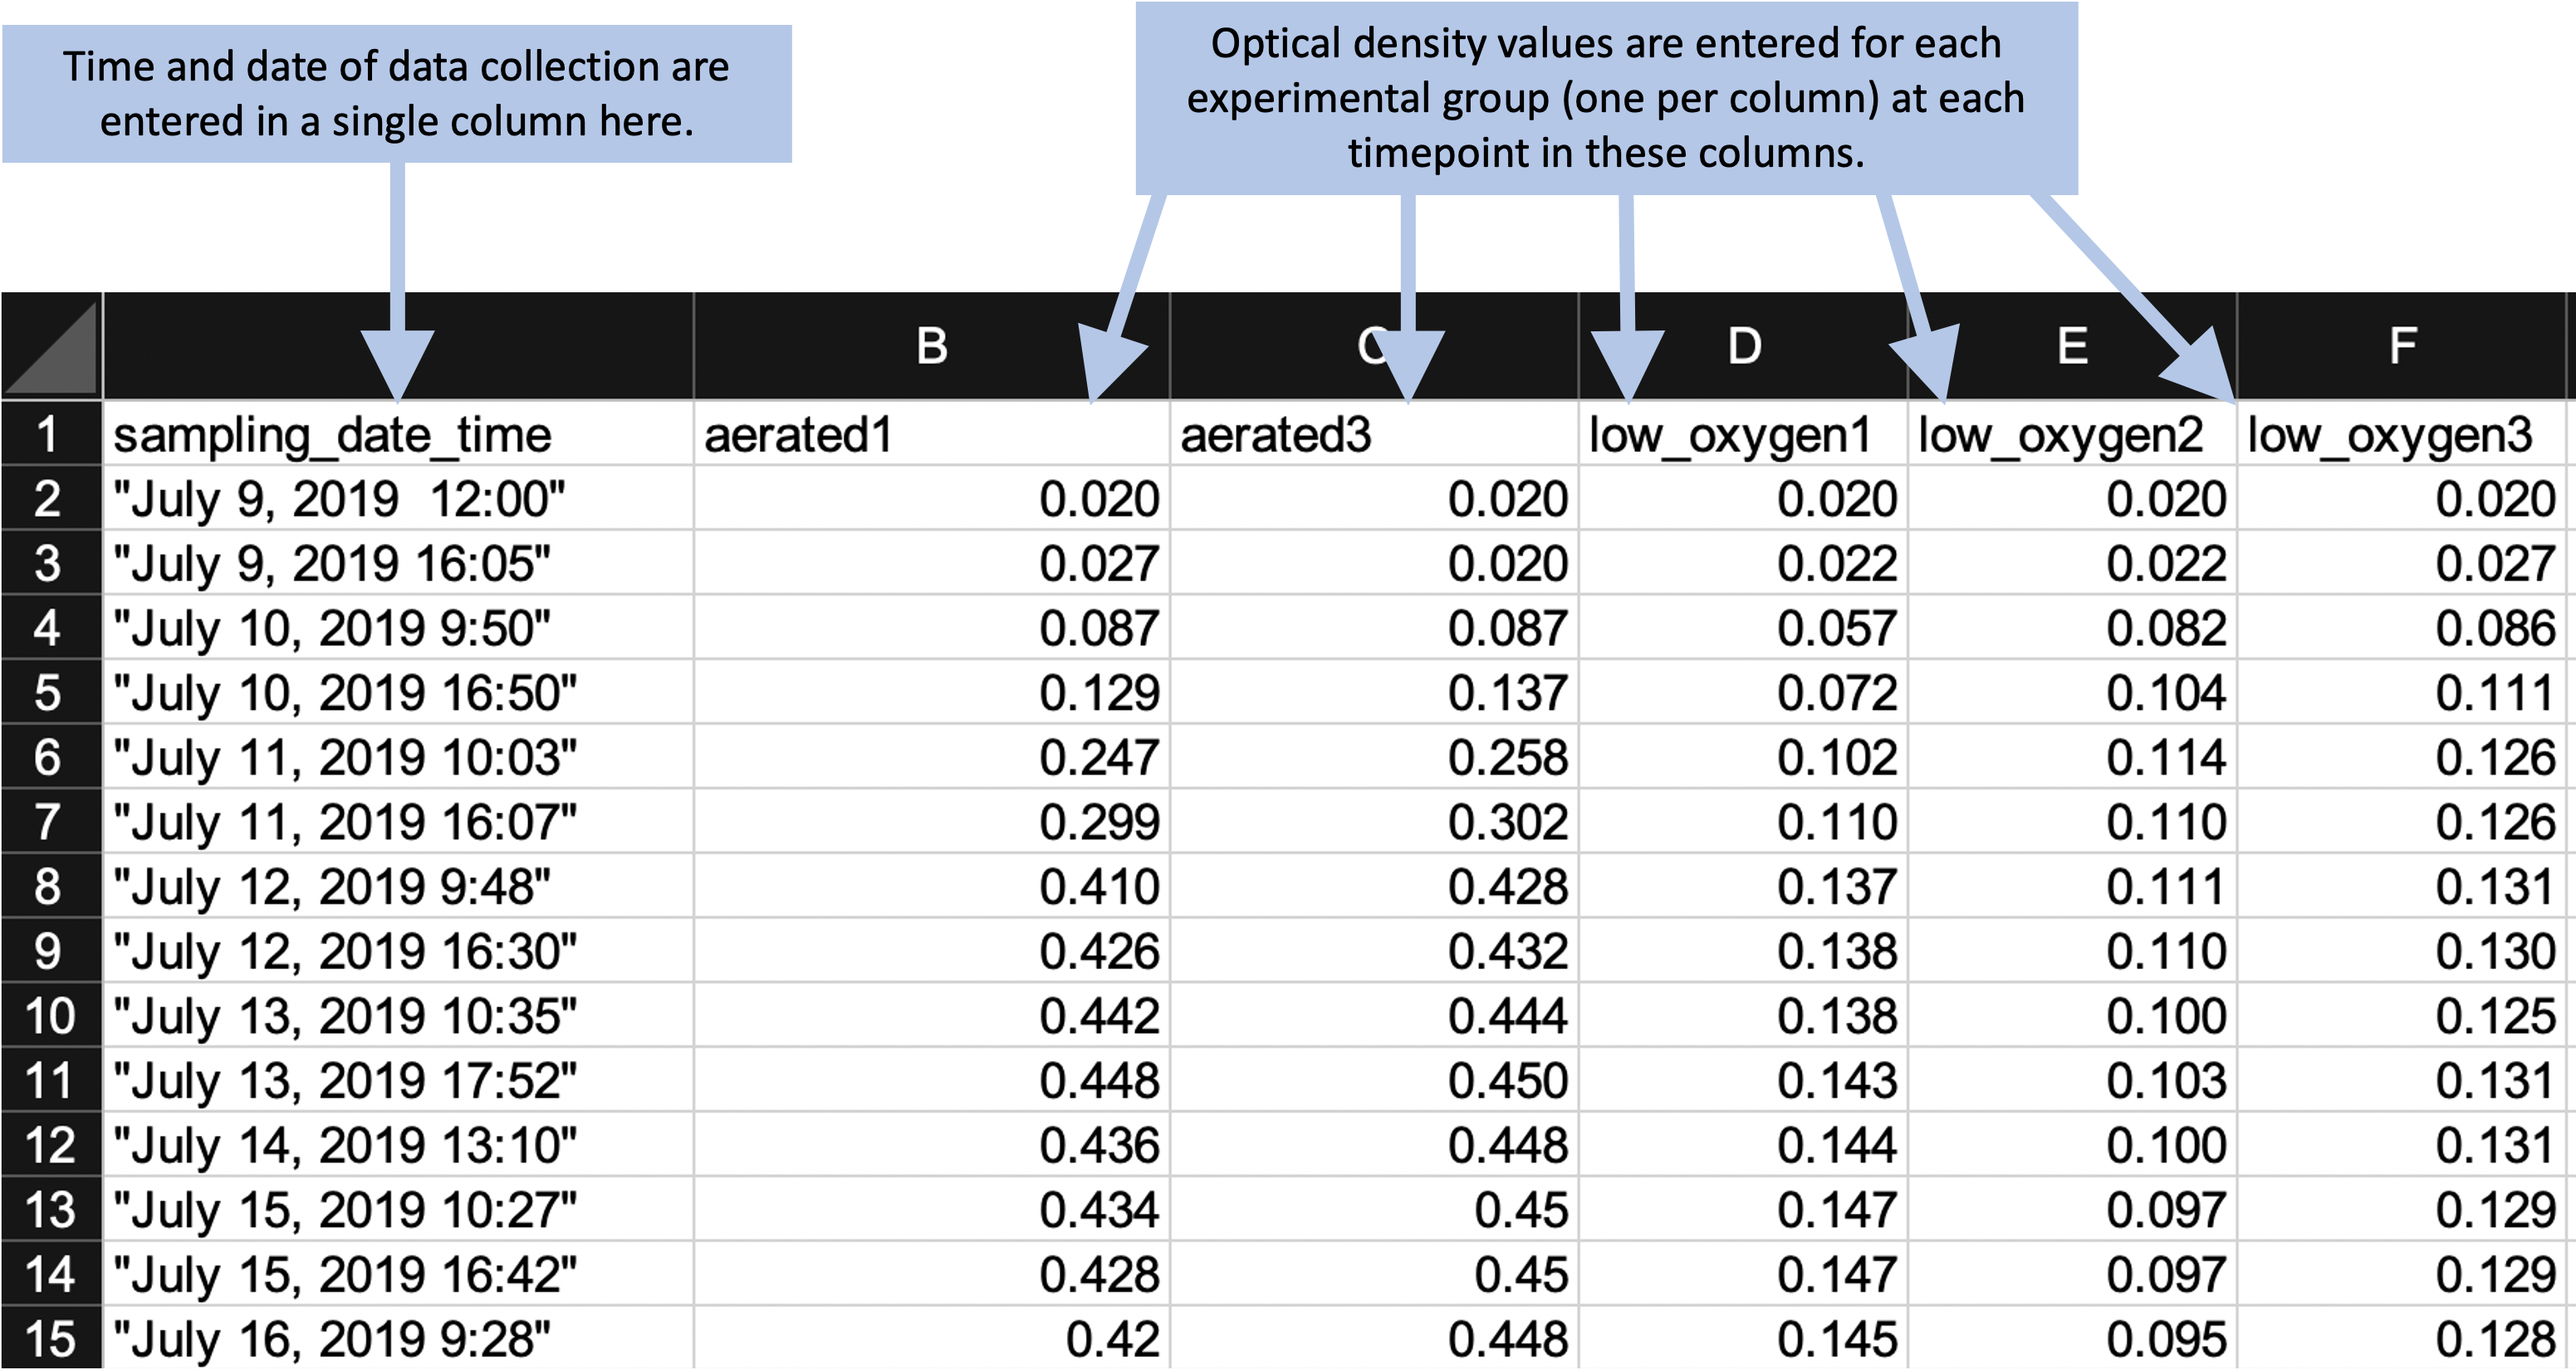
\includegraphics[width=\textwidth]{figures/growth_curve_simple} \caption[Example of an simpler format that can be used to record and analyze data for the same laboratory experiment as the previous figure]{Example of an simpler format that can be used to record and analyze data for the same laboratory experiment as the previous figure. Annotations highlight where data is entered by hand. No calculations are conducted or figures created---these are all done later, using a code script.}\label{fig:growthsimple1}
\end{figure}

By comparing these two templates, you can see that the simpler template does
not, by itself, provide immediate, real-time summaries of the collected data. The
simpler template has removed elements like plots and values calculated by embedded
formulas. At first glance, this might seem like a disadvantage of using a tidier
template to collect data. However, by combining other tools in a pipeline, it is
easy to connect the tidier raw data file to reporting tools. In this way, you can
quickly create real-time summaries of the data that are similar to those shown in
Figure \ref{fig:growthexcel1}, but that are created and reported outside the file
used to originally record the data.

\begin{figure*}
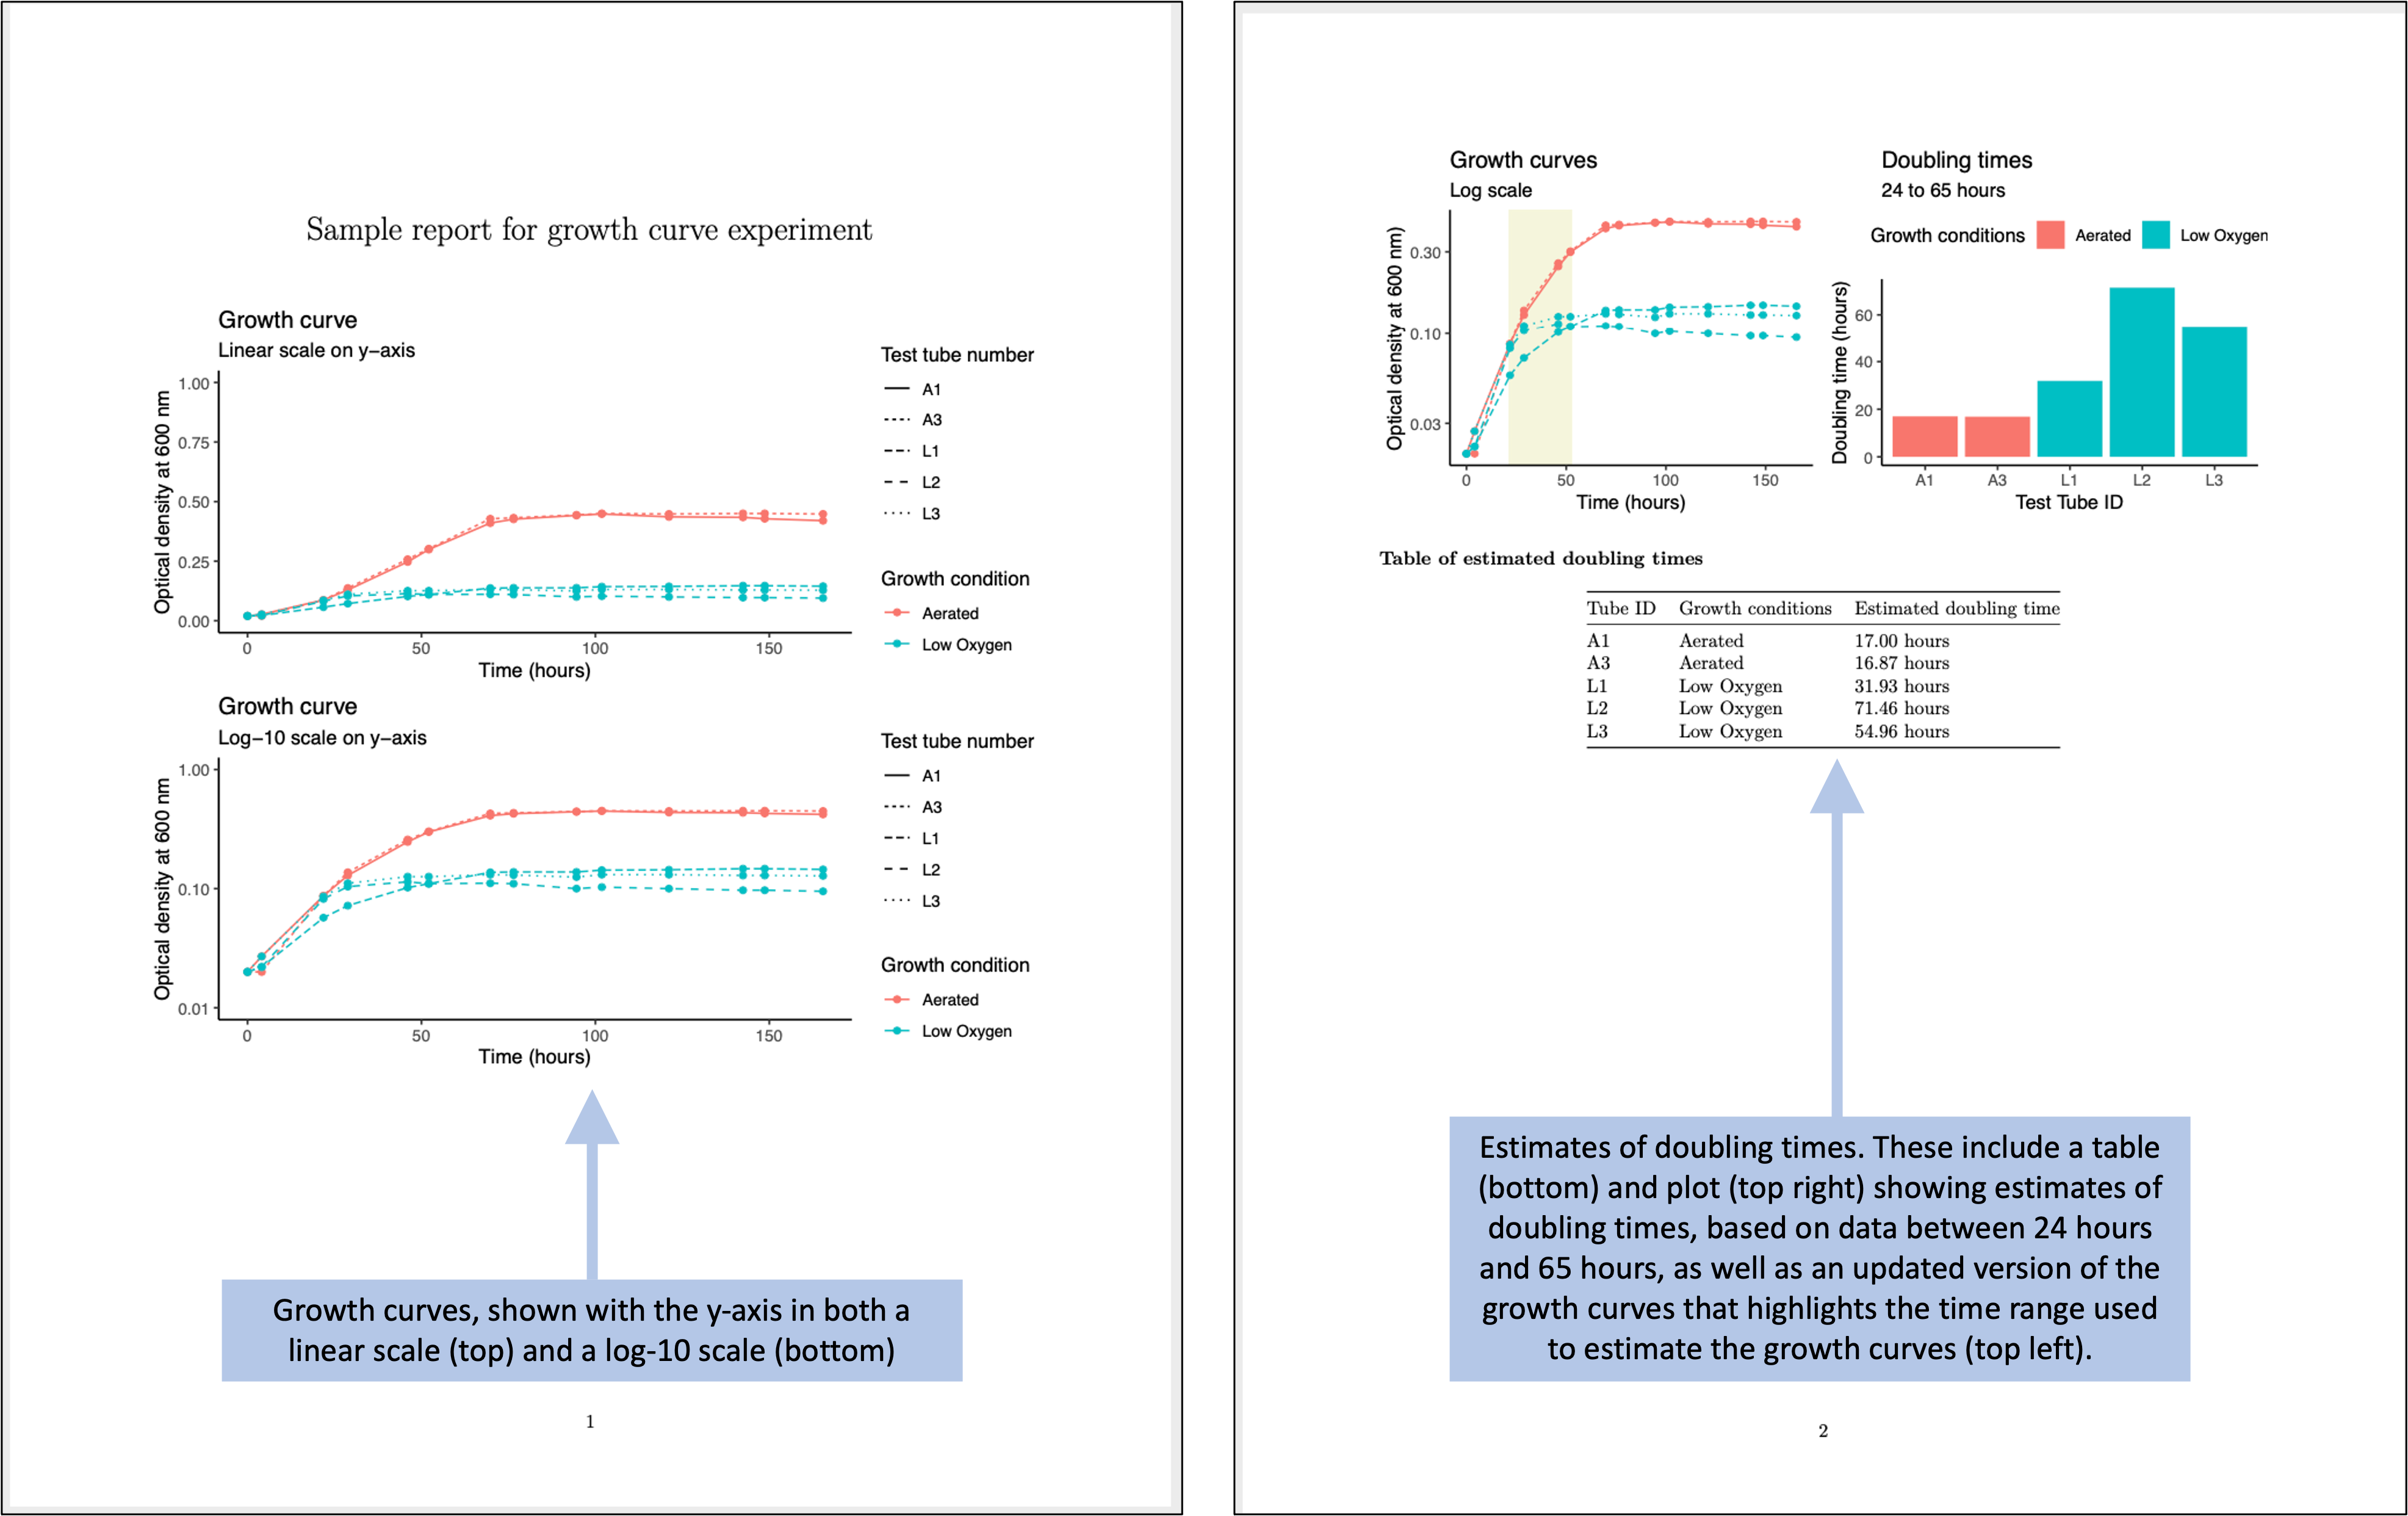
\includegraphics[width=\textwidth]{figures/growth_curve_report} \caption[Examples of an automated report that can be created to quickly generate summaries and estimates of the data collected in the simplified data collection template for the example experiment]{Examples of an automated report that can be created to quickly generate summaries and estimates of the data collected in the simplified data collection template for the example experiment.}\label{fig:growthreport1}
\end{figure*}

\hypertarget{learning-more-about-tidy-data-collection-in-the-laboratory}{%
\subsection{Learning more about tidy data collection in the laboratory}\label{learning-more-about-tidy-data-collection-in-the-laboratory}}

{[}Article with more examples on this.{]}

\begin{center}\rule{0.5\linewidth}{0.5pt}\end{center}

\textbf{Older text}

It is usually very little work to record data in a structure
that follows the ``tidy data'' principles, especially if you are planning to record
the data in a two-dimensional, tabular format already, and following these
principles can bring some big advantages. We explain these rules and provide
examples of biomedical datasets that both comply and don't comply with these
principles, to help make it clearer how you could structure a ``tidy-compliant''
structure for recording experimental data for your own research.

If the data is the same regardless of whether it's ``tidy'' or not, then why all
the fuss about following the ``tidy'' principles when you're designing the format
you'll use to record your data? The magic here ix this---if you follow these
principles, then your data can be immediately input into a collection of
powerful tools for visualizing and analyzing the data, without further cleaning
steps (as discussed in the previous module). What's more, all those tools (the
set of tools is calld the ``tidyverse'') will typically \emph{output} your data in a
``tidy'' format, as well.

Once you have tools that input and output data in the same way, it becomes very
easy to model each of the tools as ``small, sharp tools''---each one does one
thing, and does it really well. That's because, if each tool needs the same
type of input and creates that same type of output, those tools can be chained
together to solve complex problems. The alternative is to create large software
tools, ones that do a lot to the input data before giving you some output.
``Big'' tools are harder to understand, and more importantly, they make it hard
to adapt your own solutions, and to go beyond the analysis or visualization that
the original tool creators were thinking of when they created it. Think of it this
way---if you were writing an essay, how much more can you say when you can mix and
match words to create your own sentences versus if you were made to combine
pre-set sentences?

\hypertarget{creating-the-rules-for-collecting-data-in-the-same-time-each-time}{%
\subsection{Creating the rules for collecting data in the same time each time}\label{creating-the-rules-for-collecting-data-in-the-same-time-each-time}}

It is likely that there are certain types of experiments that you conduct
regularly, and that they're often trying to answer the same type of
question and generate data of a consistent type and structure. This is
a perfect chance to lay down rules or a pattern for how members of
your research group will record that data.

These rules can include:

\begin{enumerate}
\def\labelenumi{\arabic{enumi}.}
\tightlist
\item
  How many units of observation does the experiment typically have?
  Say, for example, that you are measuring the influence of two drugs on
  bactieral load in an animal at
  three time points. There may be some measurements taken at the unit of the drug
  (for example, measurements related to its chemical composition) and some
  taken at the unit of animal and time point (for example, the concentration of drug in
  an animal's blood at a certain time point). This will help you define how many
  tables you should use to collect the data---one for each unit of observation.
\item
  Which measurements will be recorded for each observation? In tidy data, the measurements
  taken for an observation are recorded in rows, so you then specify what
  column names should be used for each measurement (e.g., ``sample\_time'',
  ``animal\_weight''). If data is being recorded using multiple tables (because there
  are multiple units of observation), make sure that each table include
  ``ID'' columns that can be used to link across the tables. For example, each
  table might have a column with a unique ID for each drug being tests, or tables
  with measurements on animals might each have a column that uniquely identifies
  the animal in an observation.
\item
  What units will be used for recording each measurement? For timestamp-type
  measurments, like the date and time that an experiment started and the time of
  each sample measurement, what timezone will be used? (Even if it's always the
  same one, this can come in useful every now and then if you need to figure out
  something like whether that location's timezone followed Daylight Savings Time,
  for an experiment that spans the switch between Standard and Daylight Savings).
\end{enumerate}

{[}Figure: Three tables---measurements on a drug (chemistry), measurements on an animal (weight),
measurements on an animal at time points (drug concentration){]}

You can then take this information and design a \emph{template} for collecting that
type of data. A template is, in this case, a file that gives the ``skeleton'' of
the table or tables. You will create this template file and save it somewhere
easy for lab members to access, with a filename that makes it clear that this is
a template. For example, you may create a folder with all the templates for
tables for your experiment, and name a template in it for collecting something
like animal weights at the start of the experiment something like
``animal\_wt\_table\_template.csv'' or ``animal\_wt\_table\_template.xlsx''.
Each time someone starts an experiment collecting that type of data, he or she
can copy that template file, move it to the directory with files for that
experiment and rename it. When you open that copy of the file, you can record
observations directly into it.

{[}Figure: Example template file{]}

\begin{verbatim}
####################################################################################
####################################################################################
#
# Column names and meanings
#
# animal_id:        A unique identifier for each animal. 
# animal_wt_g:      The weight of the animal, recorded in grams. 
# date_wt_measured: The date that the animal's weight was measured, recorded as 
#                   "month day, year", e.g., "Jan 1, 2019"
# cage_id:          A unique identifier for the case in which the animal was housed
# 
# Other table templates for this experiment type: 
# drug_conc_by_time.csv: A template for recording drug concentrations in the animals
#                        by time point
# 
animal_id, animal_wt_g, date_wt_measured, cage_id
   "A101",        50.2,   "Jan 1, 2019",      "B"    
\end{verbatim}

Adding in one row of sample values, to be deleted each time the template is
copied and used, can be a very helpful addition. This will help the user remember
the formats that are expected for each column (for example, the format the
date should be recorded in), as well as small details like which columns should
include quotation marks.

These template tables can be created as flat files, like comma-separated value
files. However, if this is too big of a jump, they can also be created as
spreadsheet files. Many of the downsides of spreadsheet files are linked to
the use of embedded macros, integration of raw and processed / calculated data,
and other factors, rather than related to their use as a method to record data.
However, do note that plain text files like flat files can be opened in RStudio
in a spreadsheet-like view in RStudio. Data can be recorded directly here, in
a format that will feel comfortable for spreadsheet users, but without all the
bells and whistles that we're aiming to avoid in spreadsheet programs like Excel.

{[}Figure---Opening a csv file with a spreadsheet like view{]}

There are some advantages to shifting to record data in flat files like CSVs,
rather than Excel files, and using the spreadsheet-style view in RStudio to work
with those files if you find it easier than working with the files in a text
editor (which can get tough, since the values in a column don't always visually
line up, and you have to remember to put in the right number of columns). By
recording the data in a plain text file, you can later move to tracking changes
that are made to the data using the version control tool \emph{git}. This is a
powerful tool that can show who made changes to a file and when, with exact
details on the changes made and room for comments on why the change was made.
However, \emph{git} does not provide useful views of changes made to binary files
(like Excel), only those made in plain text files. Further, plain text files are
guaranteed to not try to ``outsmart'' you---for example, they will not try to
convert something that looks like a date into a date. Instead, they will leave
things exactly as you typed them in. Finally, later in this book we will build
up to creating templates that do even more---for example, templates for reports
you need to write and presentations you need to give, as well as templates for
the whole structure of a project. Plain text files fit very nicely into this
developing framework, while files in complex binary formats like xlxs don't fit
as naturally.

Google Sheets is another tool that might come in useful. {[}More about using this
with R.{]}

This idea of creating template files for data recording isn't
revolutionary---many laboratory groups have developed spreadsheet template files
that they share and copy to use across similar experiments that they conduct.
The difference here is in creating a table for recording data \emph{that follows the
tidy data principles}, or at least comes close to them (any steps away from
characteristics like embedded macros and use of color to record information will
be helpful).

The next chapter will walk through two examples of changing from non-tidy table
templates to ones that record data in a way that follows the tidy data
principles.

\hypertarget{subsection-1}{%
\subsection{Subsection 1}\label{subsection-1}}

\begin{quote}
``Or maybe your goal is that your data is \emph{usable} in a wide range of
applications? If so, consider adopting standard formats and metadata
standards early on. At the very least, keep track of versions of data
and code, with associated dates.'' \citep{goodman2014ten}
\end{quote}

\begin{quote}
``Standards for data include, for example, data formats, data exchange
protocols, and meta-data controlled vocabularies.'' \citep{barga2011bioinformatics}
\end{quote}

\begin{quote}
``Software systems are transparent when they don't have murky corners or hidden
depths. Transparency is a passive quality. A program is passive when it is possible
to form a simple mental model of its behavior that is actuaally predictive for all
or most cases, because you can see through the machinery to what is actually going
on.'' \citep{raymond2003art}
\end{quote}

\begin{quote}
``Software systems are discoverable when they include features that are designed
to help you build in your mind a correct mental model of what they do and how they
work. So, for example, good documentation helps discoverability to a programmer. Discoverability
is an active quality. To achieve it in your software, you cannot merely fail to be obscure,
you have to go out of your way to be helpful.'' \citep{raymond2003art}
\end{quote}

\begin{quote}
``Elegant code does much with little. Elegant code is not only correct but visibly,
\emph{transparently} correct. It does not merely communicate an algorithm to a computer,
but also conveys insight and assurance to the mind of a human that reads it. By seeking
elegance in our code, we build better code. Learning to write transparent code is a first,
long step toward learning how to write elegant code---and taking care to make code
discoverable helps us learn how to make it transparent. Elegant code is both transparent and
discoverable.'' \citep{raymond2003art}
\end{quote}

\begin{quote}
``To design for transparency and discoverability, you need to apply every tactic for
keeping your code simple, and also concentrate on the ways in which your code is a
communication to other human beings. The first questions to ask, after `Will this design
work?' are `Will it be reaadable to other people? Is it elegant?' We hope it is clear \ldots{}
that these questions are not fluff and that elegance is not a luxury. These qualities
in the human reaction to software are essential for reducing its bugginess and
increasing its long-term maintainability.'' \citep{raymond2003art}
\end{quote}

\begin{quote}
``Software is maintainable to the extent that people who are not its author can
successfully understand and modify it. Maintainability demands more than code that
works; it demands code that follows the Rule of Clarity and communicates successfully
to human beings as well as the computer.'' \citep{raymond2003art}
\end{quote}

\begin{quote}
``An equivalent to the laboratory notebook that is standard good practice in
labwork, we advocate the use of a computational diary written in the R markdown
format. \ldots{} Together with a version control system, R markdown helps with
tracking changes.'' \citep{holmes2018modern}
\end{quote}

\begin{quote}
``R.A. Fisher, one of the fathers of experimental design, is quoted as
saying `To consult the statistician after an experiment is finished is
often merely to ask him to conduct a post mortem examination. He can
perhaps say what the expierment died of.' So it is important to design an
experiment with the analysis already in mind. Do not delay thinking about
how to analyze the data until after they have been acquired. \ldots{}
Dailies: start with the analysis as soon as you have acquired some data.
Don't wait until everything is collected, as then it's too late to
troubleshoot. \ldots{} Start writing the paper while you're analyzing the data.
Only once you're writing and trying to present your results and
conclusions will you realize what you should have done properly to support
them.'' \citep{holmes2018modern}
\end{quote}

\begin{quote}
``In the same way a file director will view daily takes to correct potential
lighting or shooting issues before they affect too much footage, it is a
good idea not to wait until all runs of an experiment have been finished
before looking at the data. Intermediate data analyses and visualizations
will track unexpected sources of variation and enable you to adjust the
protocol. Much is known about the sequential design of experiments, but
even in a more pragmatic setting it is important to be aware of your sources
of variation as they occur and adjust for them.'' \citep{holmes2018modern}
\end{quote}

\begin{quote}
``Analysis projects often begin with a simple script, perhaps to try out a
few initial ideas and explore the quality of the pilot data. Then more ideas are
added, more data come in, other datasets are integrated, more people become
involved. Eventually the paper need to be written, the figures need to be done
`properly' and the analysis needs to be saved for the scientific record and
to document its integrity.'' \citep{holmes2018modern}
\end{quote}

\begin{quote}
``\textbf{Use literate programming tools.} Examples are Rmarkdown and Jupyter. This
makes code more readable (for yourself and for others) than burying
explanations and usage instructions in comments in the source code or in
separate README files. In addition, you can directly embed figures and tables
in these documents. Such documents are good starting points for the supplementary
material of your paper. Moreover, they're great for reporting analyses to your
collaborators.'' \citep{holmes2018modern}
\end{quote}

\hypertarget{dont-repeat-yourself}{%
\subsection{Don't Repeat Yourself!}\label{dont-repeat-yourself}}

One of the core tenets of programming is the philosophy of ``Don't Repeat
Yourself'' (a.k.a., the ``DRY Principle'').{[}Source of ``Don't Repeat
Yourself''---\emph{The Pragmatic Programmer}{]} With programming, you can invest a
little bit of time to code your computer to do things that take a lot of your
time otherwise. In this way, you can automate repetitive tasks.

\begin{quote}
``The DRY principle, for Don't Repeat Yourself, is one of the colloquial tenets
of programming. That is, you should name things once, do things once, create a
function once, and let the computer repeat itself.'' {[}ford2015code{]}
\end{quote}

\begin{quote}
``Code, in other words, is really good at making things \emph{scale}. Computers
may require utterly precise instructions, but if you get the instructions
right, the machine will tirelessly do what you command over and over and
over again, for users around the world. \ldots{} Solve a problem once, and you've
solved it for everyone.'' {[}Coders, p.~20{]}
\end{quote}

\begin{quote}
``Since they have, at their beck and call, machines that can repeat
instructions with robotic perfection, coders take a dim view of doing
things repetitively themselves. They have a dislike of inefficiency
that is almost aesthetic---they recoil from it as if from a disgusting
smell. Any opportunity they have to automate a process, to do something
more efficiently, they will.'' {[}Coders, p.~20{]}
\end{quote}

\begin{quote}
``Programmers are obsessed with efficiency. \ldots{} Removing the friction
from a system is an aesthetic joy; {[}programmers'{]} eyes blaze when they
talk about making something run faster, or how they eliminated some
bothersome human effort from a process.'' {[}Coders, p.~122{]}
\end{quote}

\begin{quote}
``Computers, in many ways, inspire dreams of efficiency greater than
any tool that came before. That's because they're remarkably good at
automating repetitive tasks. Write a script once, set it running, and
the computer will tirelessly execute it until it dies or the power
runs out. What's more, computers are strong in precisely the ways that
humans are weak. Give us a repetitive task, and our mind tends to
wander, so we gradually perform it more and more irregularly. Ask us
to do something at a precise time or interval, and we space out and
forget to do it. \ldots{} In contrast, computers are clock driven and superb
at doing the same thing at the same time, day in and day out.''
{[}Coders, p.~124{]}
\end{quote}

\begin{quote}
``Larry Wall, the famous coder and linguist who created the Perl
programming language, deeply intuited this coderly aversion to
repetition. In his book on Perl, he and coauthors wrote that one of the
key virtues of a programmer is `laziness'. It's not that you're too lazy
for coding. It's that you're too lazy to do routine things, so it
inspires you to automate them.'' {[}Coders p.~126{]}
\end{quote}

In scientific research, there are a lot of these repetitive tasks, and as tools for
automation continue to develop, there are many opportunities to ``automate away'' busywork.

\begin{quote}
``Science often involves repetition of computational tasks such as processing
large number of data files in the same way or regenerating figures each time
new data are added to an existing analysis. Computers were invented to do these
kinds of repetitive tasks but, even today, many scientists type the same
commands in over and over again or click the same buttons repeatedly.'' {[}wilson2014best{]}
\end{quote}

\begin{quote}
``Whenever possible, rely on the execution of programs instead of manual procedures
to modify data. Such manual procedures are not only inefficient and error-prone,
they are also difficult to reproduce.'' {[}sandve2013ten{]}
\end{quote}

\begin{quote}
``Other manual operations like the use of copy and paste between documents should
also be avoided. If manual operations cannot be avoided, you should as a minimum
note down which data fiels were modified or moved, and for what purpose.'' {[}sandve2013ten{]}
\end{quote}

Statisticians have been doing this for a while for data cleaning analysis tasks.
For example, if you need to read in an Excel file into a statistical programming
language like R, you could write a few lines of code to do that anew each time
you get a new file. However, say you get Excel files over and over that follow
the same format--for example, files with the same number of columns, the same
names for those columns, and the same type of data. You can write a \emph{script}---a
recorded file with a few lines of code, in this case---that reads in the file.
You can apply this script to each new file.

This saves you a little bit of time. It also ensures that you do the exact same thing
with every file you get. It also means that you can reproduce what you do now to a file
in the future. Say, for example, that you are working on a project and you read in a file
and conduct an analysis. Your laboratory group sends the paper out for review. Months
later, you get back comments from the reviewers, and they are wondering what would
happen if you had analyzed the data a bit differently---say, used a different
statistical test. If you use a script to read in the data file, then when you re-run
it to address the reviewers' comments, you can be sure that you are getting your
data into the statistical program in the exact same way you did months ago, and so
you're not unintentionally introducing differences in your results because you
are doing some small things differently in processing the file.

This idea can extend across the full data analysis you do on a project. You are only
saving a little bit of time and effort, maybe, by automating the step where you read
the data from a spreadsheet into the statistical program. And it takes some time to
write that script the first time, so it can be tempting to do it fresh each time you
need to do it. However, you can also write scripts that will automate cleaning your data.
Maybe you want to identify data points with very high (maybe suspect) values for a certain
measurement, or remove observations with missing data. You can also write scripts that
will automating processing your data---doing things like calculating the time since the
start of an experiment based on the recorded sampling time for an observation. Each of
these steps might be small, but the time saved really adds up since you typically
need to perform many of these steps each time you run a new experiment.

There are many cases in life where you'll need to make the choice between spending
some time upfront to make something more efficient, versus doing it more quickly the first
time but then having to do it ``from scratch'' again each following time. For example,
say that you're teaching a class, and you need to take attendance for each class period.
You could write down the names of each student at the first class and save that, and
then the next class write down the name of each student who shows up that day on a separate
sheet of paper, and so on for each class meeting. Conversely, you could take some extra
time before the first class and create a table or spreadsheet file with every student's
name and the date of each class, and then use that to mark attendance. The first method
will be quicker the first day, but more time consuming each following time. The second
method requires a small initial investment, but with time-saving returns in the following
class meetings.

For people who use scripts and computer programs to automate their data-related tasks,
it quickly becomes very confusing how anyone who doesn't could argue that they don't because
they don't have time to learn how to. The amount of time you end up saving based on your
initial investment is just so high if you're working with data, that it would have to take
a huge time investment to not be worth it. Plus---the thrill of running something that you've
automated! It's a very similar feeling to the feeling you get when a student or postdoc that
you've spent a lot of time training has gotten to the point where you can just ask them
to run something, and they do, and it means you don't have to.

Here are some of the problems that are solved by automating your small tasks:

\begin{enumerate}
\def\labelenumi{\arabic{enumi}.}
\item
  \textbf{It gets done the same way every single time.} Even simple tasks can be done with
  numerous small modifications. You will probably remember some of those choices and
  settings and modifications the next time you need to do the same thing, but probably
  not all of them, and so those choices will not be exact from one time to the next.
  If the computer is doing it based on a clear set of instructions, it will be.
\item
  \textbf{It gets done more quickly.} Or if not more quickly (some large data might take
  some time to process), at least the spent time is the computers time, not yours. You
  can leave the computer to run the script while you get on with other things that
  a computer can't do.
\item
  \textbf{Anyone who does it can do it the same way.} Just as you might not do something
  exactly the same way from one time to the next, one person in a laboratory group is
  likely to do things at least slightly different than other members of the group.
  Even with very detailed instructions, few instructions written for humans can be
  so detailed and precise to ensure that something is done exactly the same way by
  everyone who follows them. If everyone is given the same computer script to run,
  however, and they all instruct the computer to run that script, the task will be
  done in exactly the same way.
\item
  \textbf{It is easier teach new people how to do the task.} Often, with a script to
  automate a task, you just need to teach someone new to the laboratory group how
  to get the computer to run a script in a certain language. When you need them to
  run a new script, the process will be the same. The script encapsulates all the
  task-specific details, and so the user doesn't need to understand all of them to
  get something to run. What's more, once you want to teach a new lab member how
  everything it working, so they can understand the full process, the script provides
  the exact recipe. You can teach them how to read and understand scripts in that
  language, and then the scripts you've created to automate tasks serve as a recipe
  book for everything going on in terms of data analysis for the lab.
\item
  \textbf{You can create tools to share with others.} If you've written a script that's
  very useful, with a bit more work you can create it into a tool that you can share
  with other research groups and perhaps publish a paper about. Papers about R
  software extensions (also called \emph{packages}) and data analysis workflows and
  pipelines are becoming more and more common in biological contexts.
\item
  \textbf{It's more likely to be done correctly.} Boring, repetative tasks are easy
  to mess up. We get so bored with them, that we shift our brains into a less-attentive
  gear when we're working on them. This can lead to small, stupid mistakes, ones
  at the level of typos but that, with data cleaning and analysis, can have much
  more serious ramifications.
\end{enumerate}

\begin{quote}
``We view workflows as a paradigm to: 1) expose non-experts to well-understood
end-to-end data analysis processes that have proven successful in challenging
domains and represent the state-of-the-art, and 2) allow non-experts to easily
experiment with different combinations of data analysis processes, represented
as workflows of computations that they can easily reconfigure and that the
underlying system can easily manage and execute.'' {[}hauder2011making{]}
\end{quote}

\begin{quote}
``While reuse {[}of workflows{]} by other expert scientists saves them time and
effort, reuse by non-experts is an enabling matter as in practice they would
not be able to carry out the analytical tasks without the help of
workflows.'' {[}hauder2011making{]}
\end{quote}

\begin{quote}
``We observed that often steps that could be easily automated were performed manually
in an error-prone fashion.'' {[}vidger2008supporting{]}
\end{quote}

Biological research is quickly moving where a field where projects often required
only simple and straightforward data analysis once the experimental data was
collected---with the raw data often published directly in a table in the manuscript---to
a field with very complex and lengthy data analysis pipelines between the experiment
and the final manuscript. To ensure rigor and clarity in the final research results,
as well as to allow others to reproduce the results exactly, the researcher must
document all details of the computational data analysis, and this is often
missing from papers. RMarkdown documents (and their analogues) can provide all these
details unambiguously---with RMarkdown documents, you can even run a command to
pull out all the code used within the document, if you'd like to submit that
code script as a stand-alone document as a supplement to a manuscript.

\begin{quote}
``More recently, scientists who are not themselves computational experts are
conducting data analysis with a wide range of modular software tools and packages.
Users may often combine these tools in unusual or nove ways. In biology,
scientists are now routinely able to acquire and explore data sets far beyond
the scope of manual analysis, including billions of DNA bases, millions of genotypes,
and hundreds of thousands of RNA measurements. \ldots{} While propelling enormous
progress, this increasing and sometimes `indirect' use of computation poses
new challenges for scientific publication and replication. Large datasets are
often analyzed many times, with modifications to the methods and parameters, and
sometimes even updates of the data, until the final results are produced. The
resulting publication often gives only scant attendtion to the computations details.
Some papers have suggested these papers are `merely the advertisement of
scholarship whereas computer programs, input data, parameter values, etc., embody
the scholarship itself.' However, the actual code or software `mashup' that
gave rise to the final analysis may be lost or unrecoverable.'' {[}mesirov2010accessible{]}
\end{quote}

\begin{quote}
``Bioinformatic analyses invariably involve shepherding files through a series
of transformations, called a pipeline or workflow. Typically, these transformations
are done by third-part executable command line software written for Unix-compatible
operating systems. The advent of next-generation sequencing (NGS), in which millions
of short DNA sequences are used as the source input for interpreting a range of
biological phenomena, has intensified the need for robust pipelines. NGS analyses
tend to involve steps such as sequence alignment and genomic annotation that are
both time-intensive and parameter-heavy.'' {[}leipzig2017review{]}
\end{quote}

\begin{quote}
``\textbf{Rule 7: Always Store Raw Data behind Plots.} From the time a figure is first
generated to it being part of a published article, it is often modified several
times. In some cases, such modifications are merely visual adjustments to
improve readability, or to ensure visual consistency between figures. If raw data
behind figures are stored in a systematic manner, so as to allow raw data for
a given figure to be easily retrieved, one can simply modify the plotting
procedure, instead of having to redo the whole analysis. An additional
advantage of this is that if one really wants to read fine values in a figure,
one can consult the raw numbers. \ldots{} When plotting is performed using a
command-based system like R, it is convenient to also store the code
used to make the plot. One can then apply slight modifications to these
commands, instead of having to specify the plot from scratch.'' {[}sandve2013ten{]}
\end{quote}

\hypertarget{dont-repeat-your-report-writing}{%
\subsection{Don't repeat your report-writing!}\label{dont-repeat-your-report-writing}}

Until a few years ago, statisticians and data analysts frequently automated the
data cleaning, processing, and analysis tasks. But that still left the paper
and report writing to be done by hand. This process is often repetitive. You would
do your analysis and create some tables or figures. You would save these from
your statistical program and then paste them into your report or paper draft.
If you decided that you needed to change your analysis a bit, or if you got a new
set of data to analyze in a similar way, you had to go back to the statistical
program, run things again there, save the tables and figure files again, and paste
them in the report or paper again to replace the outdated version. If there were
numbers from the analysis in the text of the paper, then you had to go back through
the text and update all of those with the newer numbers, too.

Do you still write your papers and reports like this? I can tell you that there is
now a \emph{much} better way. Computer scientists and other programmers started thinking
quite a while ago about how to create documents that combine computer code and
text for humans, and to do it in a way where the computer code isn't just a static
copy of what someone once told the computer to do, but instead a living, working,
\emph{executable} set of instructions that the computer can run anytime you ask it to.

These ideas first perculated with Donald Knuth, who many consider to be the greatest
computer programmer of all time {[}Bill Gates, for example, has told anyone who reads Dr.~Knuth's
magnum opus, \emph{The Art of Computer Programming}, to come see him right away about a job{]}.
As Dr.~Knuth was writing a book on computer programming, he became frustrated with the
quality of the typesetting used in the final book. In a field that requires a lot of mathematical
and other symbols incorporated into the text, it takes a bit more to make an attractive
book than with simpler text. Dr.~Knuth therefore took some time to create a programming
for typesetting. (You may have heard of it---if you ever notice that a journal's
Instructions to Authors allow authors to submit articles in ``LaTeX'' or ``TeX'', that's
using a system built off of Donald Knuth's typesetting program.)

And \emph{then}, once he had that typesetting program, he started thinking about how
programmers document their code. When one person does a very small code project,
and that one person is the only person who will ever go back to try to modify or
understand the code, that person might be able to get away with poor
documentation in the code. However, interesting code projects can become
enormous, with many collaborators, and it becomes impossible to understand and
improve the code if it doesn't include documentation explaining, in human terms,
what the code is doing at each step, as well as some overall documentation
explaining how different pieces of the code coordinate to get something big
done.

Traditionally, code was documented by including small comments within the code. These comments
are located near the code that they explain, and the order of the information in the
code files are therefore dominated by the order of the instructions to the computer,
not the order that you might explain what's going on to a human. To ``read'' the code and
the documentation, you end up hopscotching through the code, following the code inside
one function when it calls another function, for example, to where the code for that
second function is defined and then back to the first, and so on. You often follow paths as
you get deeper and deeper into helper functions and the helper functions for those functions,
that you feel like you're searching through a set of Russian dolls and then coming back up
to start on a new set of Russian dolls later down the line.

Donald Knuth realized that, with a good typesetting program that could itself be programmed,
you could write your code so that the documentation for humans took precedence, and could
be presented in a very clear and attractive final document, rather than hard-to-read
computer code with some plain-text comments sprinkled in. Computers don't care what order
the code is recorded in---as long as you give them some instructions on how to decipher
code in a certain format or order, they can figure out how to use it fine. But human brains
are a bit more finicky, and we need clear communication, laid out in a logical and helpful
order. Donald Knuth created a paradigm of \emph{literate programming} that interleaved
executable code inside explanations written for humans; by making the code executable, it
meant that the document was a living guide. When someone changed the program, they did
it by changing the documentation---documentation wasn't left as the final, often neglected,
step to refine once the ``real code'' was written (and the ``real work'' done).

\begin{quote}
``Programs must be written for people to read, and only incidentally for machines
to execute. A great program is a letter from current you to future you or
the the person who inherits your code. A generous humanistic document.'' {[}ford2015what{]}
\end{quote}

Well, this was a fantastic idea. It hasn't been universely leveraged, but the projects that
do leverage it are much stronger for it. But that's not where the story ends. If you are
someone who does a little bit of coding (maybe small scripts to analyze and visualize your
data, for example) and a lot of ``documenting'' of the results, and if you're not planning
on doing a lot of large coding projects or creating software tools, it's not immediately
how you'd use these literate programming ideas.

Well, there are many people who do a little bit of programming in service to a larger
research project. While they are not creating software that needs classical software
documentation, they do want to document the results that they get when they run their
scripts, and they want to create reports and journal articles to share what they've
found. Several people took the ideas behind literate programming---as it's used to
document large software projects---and leveraged it to create tools to automate
writing in data-related fields.

{[}F. Leisch?{]} was the first to do this with the R programming language, with a
tool called ``Sweave'' (``S''-``weave'', as R builds off of another programming
language called ``S'' and Leisch's program would ``weave'' together S / R code and
writing). This used Donald Knuth's typesetting program. It allowed you to write
a document for humans (like a report or journal article) and to intersperse bits
of code in the paper. You'd put each code piece in the spot in the paper where
the text described what was going on or where you wanted the results that it
generated for example, if you had a section in the Methods where you talked
about removing observations that were outliers, you would add in the code that
took out those outliers right there in the paper. And if you had a placed in the
Results that talked about how your data were different between two experimental
groups, you would add the code that generated the plot to show that right there
in the paper.

To tell the computer how to tell between code and writing, you would add a little
weird combination of text each time that you wanted to ``switch'' into code and then
another one each time you wanted to switch back into writing for humans. (These
combinations were so weird because that guaranteed that it was a combination you
would probably never want to type otherwise, so you wouldn't have a lot of
cases of the computer getting confused between whether the combo meant to switch
to code or whether it was just something that came up in the regular writing.)
You'd send the document, code and writing and all, through R once you had it
written up. R would ignore everything that wasn't code. When it got to the code
pieces, it would run them, and if the code created output (like a figure or table),
it would ``write'' that into the document at that point in the text. Then you'd run
the document through Donald Knuth's typesetting program (or an extension of it),
and the whole document would get typeset into an attractive final product (often
a pdf, although you had some choices on the type of output).

This meant that you got very attractive final documents. It also meant that your
data analysis code was well documented---it was ``documented'' by the very article
or report you wrote based on it, because the code was embedded right there in the
final product! It also meant that you could save a lot of time if you needed to
go back and change some of your code later (or input a different or modified dataset).
You just had to change that small piece of code or data input, and then essentially
press a button to put everything together again, and the computer would re-write the
whole report for you, with every figure and table updated. It even let you write
small bits of computer code directly into the written text, in case you need to
write something like ``this study included 52 subjects'', where the ``52'' came from
you counting up the number of rows in one of your datasets---if you later added three
more subjects and re-ran the analysis with the updated dataset, the report would
automatically change to read ``this study included 55 subjects''.

Leisch's system is still out there, but another has been adopted much more
widely, building on it. Yihui Xie started work on a program that tweaked and
improved Leisch's Sweave program, creating something called ``knitr''
(``knit''-``R''---are you noticing a pattern in the names?). Xie's knitr program,
along with its extensions, is now widely used for data analysis projects. What's
more, it's grown to allow for larger or more diverse writing projects---this
book, for example, is written using an extension called ``bookdown'', and
extensions also exist for create blogs that include executable R code
(``blogdown'') and websites with documentation for R packages (``packagedown'').

So now, let's put these two pieces together. We know that programmers love to
automate small tasks, and we know that there are tools that can be used to
``program'' tasks that involve writing and reporting. So what does this mean if
you frequently need to write reports that follow a similar pattern and start
from similar types of data? If you are thinking like a code, it means that
you can move towards automating the writing of those reports.

One of us was once talking to someone who works in a data analysis-heavy field,
and she was talking about how much time she spends copying the figures that her
team creates, based on a similar analysis of new data that's regularly
generated, into PowerPoint presentations. So, for this weeks report, she's
creating a presentation that shows the same analysis she showed last week, just
with newer data. Cutting and pasting is an enormous waste of time---there are
tools to automate this.

\hypertarget{automating-reports}{%
\subsection{Automating reports}\label{automating-reports}}

First---think through the types of written reports or presentations you've
created in the past year or two. Are there any that follow a similar pattern?
Any that input the same types of data, but from different experiments, and then
report the same types of statistics or plots for them? Are there Excel
spreadsheets your lab uses that generate specific tables or plots that you often
cut and paste for reports or presentations? Look through your computer file
folders or email attachments if you need to---many of these might be small
regular reports that are so regular that they don't pop right to mind. If you
are creating documents that match any of these conditions, you probably have
something ripe for converting to a reusable, automatable template.

\begin{quote}
``Think like Henry Ford; he saw that building cars was a repeatable process and
came up with the moving assembly line method, revolutionizing production. You
may not be building a physical product, but chances are you are producing something.
\ldots{} Look for the steps that are nearly identical each time, so you can build your
own assembly line.'' {[}rose2018dont{]}
\end{quote}

\ldots{} {[}Creating a framework for the report{]}

\begin{quote}
``Odds are, if you're doing any kind of programming, especially Web programming,
you've adopted a framework. Whereas an SDK is an expression of a corporate
philosophy, a framework is more like a product pitch. Want to save time? Tired
of writing old code? Curious about the next new thing? You use a graphics
framework to build graphical applications, a Web framework to build Web
applications, a network framework to build network servers. There are
hundreds of frameworks out there; just about every language has one.
A popular Web framework is Django, which is used for coding in Python.
Instagram was bootstrapped on it. When you sit down for the first time
with Django, you run the command `startproject', and it makes a directory
with some files and configuration inside. This is your project directory. Now
you have access to libraries and services that add to and enhance the standard
library.'' {[}ford2015what{]}
\end{quote}

One key advantage of creating a report template is that it optimizes the time of
statistical collaborators. It is reasonable for a scientists with a couple of
courses worth of statistical training to design and choose the statistical tools
for simple and straightforward data analysis. However, especially as the
biological data collected in experiments expands in complexity and size, a
statistician can recommend techniques and approaches to draw more knowledge
from the data and to appropriately handle non-standard features of the data.
There is substantial work involved in the design of any data analysis pipeline
that goes beyond the very basics. It waste time and resources to recreate this
with each new project, time that---in the case of statistical collaborators---could
probably be better spent in extending data analysis goals beyond the simplest
possible analysis to explore new hypotheses or to add exploratory analysis that
could inform the design of future experiments.

\begin{quote}
``Workflows effectively capture valuable expertise, as they represent how an
expert has designed computational steps and combined them into an
end-to-end process.'' {[}hauder2011making{]}
\end{quote}

When collaborative work between scientists and statisticians can move towards
developing repeatable data analysis scripts and report templates, you will start
to think more about common patterns and common questions that you ask across
many experiments in your research program, rather than focusing on the immediate
needs for a specific project. You can start to think of the data analysis tools
that are general purpose for your research lab, develop those into clean,
well-running scripts or functions, and then start thinking about more
sophisticated questions you want to ask of your data. The statisticians you
collaborate will be able to see patterns across your work and help to develop
global, and perhaps novel, methods to apply within your research program, rather
than piecemeal small solutions to small problems.

\begin{quote}
``Although foundational knowledge is taught in major universities and colleges,
advanced data analytics can only be acquired through hands-on practical training.
Only exposure to real-world datasets allows students to learn the importance of
preparing and cleansing the data, designing appropriate features, and
formulating the data mining task so that the data reveals phenomena of interest.
However, the effort required to implement such complex multi-step data analysis
systems and experiment with the tradeoffs of different algorithms and feature
choices is daunting. For most practical domains, it can take weeks to months for
a student to setup the basic infrastructure, and only those who have access to
experts to point them to the right high-level design choices will endeavor on
this type of learning. As a result, acquiring practical data analytics skills
is out of reach for many students and professionals, posing severe limitations
to our ability as a society to take advantage of our vast digital data resources.''
{[}hauder2011making{]}
\end{quote}

\begin{quote}
``In practice designing an appropriate end-to-end process to prepare and analyze the
data plays a much more influential role than using a novel classifier or
statistical model.'' {[}hauder2011making{]}
\end{quote}

It is neither quick nor simple to design the data analysis plan and framework
for a research experiment. It is not simply naming a statistical test or two.
Instead, the data analyst must start by making sure they understand the data,
how it was measured, how to decipher the format in which it's stored, what
questions the project is hoping to answer, where there might be problems in the
data (and what they would look like), and so on. If a data analyst is helping
with a lot of projects using similar types of data to answer similar questions,
then he or she should, in theory, need less time for these ``framework'' types of
questions and understanding. However, if data isn't shared in the same format
each time, it will still take overhead to figure out that this is indeed the
same type of data and that code from a previous project can be adapted or
repurposed.

Let's think about one area where you likely repeat very similar steps
frequently---writing up short reports or slide presentations to share your
to-date research results with your research group or colleagues. These
probably often follow a similar structure. For example, they may start with
a section describing the experimental conditions, and then have a slide
showing a table with the raw data (or a simple summary of it, if there's a lot
of data), and then have a figure showing something like the difference in
experimental measurements between to experimental groups.

{[}Figure: Three simple slides for a research update---experimental conditions,
table of raw data, boxplots with differences between groups.{]}

\begin{quote}
``The cornerstone of using DRY in your work life is the humble template.
Whenever you create something, whether it's an email, a business document,
or an infographic, think if there's something there you could save for
future use. The time spend creating a template will save you exponentially
more time down the road.'' {[}rose2018dont{]}
\end{quote}

You could start very simply in turning this into a template. You could start by
creating a PowerPoint document called ``lab\_report\_template.pptx''. It could
include three slides, with the titles on each slide of ``Experimental
conditions'', ``Raw data'', and ``Bacterial burden by group'', and maybe with some
template set to provide general formatting that you like (font, background
color, etc.). That's it. When you need to write a new report, you copy this file,
rename the copy, and open it up. Now instead of needing to start from a blank
PowerPoint file, you've shaved off those first few steps of setting up the
pieces of the file you always use.

{[}Figure: Simplest possible template{]}

This very simple template won't save you much time---maybe just a minute or so for
each report. However, once you can identify other elements that you commonly use
in that type of report, you can add more and more of these ``common elements'' to the
template, so that you spend less time repeating yourself with each report. For
example, say that you always report the raw data using the same number of columns
and the same names for those columns. You could add a table to that slide in your
template, with the columns set with appropriate column names. You can always add or
delete rows in the table if you need to in your reports, but now each time you
create a new report, you save yourself the time it takes to create the table
structure and add the column names. Plus, now you've guaranteed that the first
table will use the exact same column names every time you give a report! You'll never
have to worry about someone wondering if you are using a different model animal
because you have a column named ``Animal ID'' in one report, while your last report
had ``Mouse ID'', for example. And because you're making a tool that you'll use many
times, it becomes worthwhile to take some time double-checking the clean-up, so
you're more likely to avoid things like typos in the slide titles or in columns names
of tables.

{[}Figure: Template with a table skeleton added.{]}

You can do the same thing for written reports or paper manuscripts. For example,
most of the papers you like may have the classic scientific paper sections: ``Introduction'',
``Data and Methods'', ``Results'', and ``Discussion''. And then, you probably typically include
a couple of pages at the beginning for the title page and abstract, and then a section
at the end with references and figure captions. Again, you could create a file called
``article\_template.docx'' with section headings for each of the sections and with space for
the title page, abstract, and references. Presumably, you are always an author on papers you're
writing, so go ahead and add your name, contact information, and affiliation in the right
place on the title page (I bet you have to take the time to do that every time you start
a paper---and if you're like me, you have to look up the fax number for your building
every time you do). You probably need to mention funding sources on the title page for
every paper, too. Do you need to look those grant numbers up every time? Nope! Just
put all your current ones in the title page of your template, and then you can just
delete those that don't apply when you start a new paper.

{[}Figure: Simple article template{]}

Again, you can build on this simple template. Look through the ``Data and Methods''
section of several of your recent papers. Are there certain elements that you commonly
report there? For example, is there a mouse model you use in most of your experiments,
that you need to describe? Put it in the template. Again, you can always delete or
modify this information if it doesn't apply to a specific paper. But for any information
that you find yourself copying and pasting from one paper draft to another, add it to
your template. It is so much more delightful to start work on a paper by \emph{deleting} the
details that don't apply than by staring down a blank sheet of paper.

{[}Quote---Taking away everything that isn't the statue.{]}

\begin{quote}
``Most docs you work on will have some sort of repeatable process. For example,
when I sit down to write a blog post, I go through the same repeatable steps when
setting up my file: Title, Subtitle, Focus Keywords, Links to relevant articles /
inspiration, Outline of subheds, Intro / hook, etc. \ldots{} Even though it is a
well-worn process, I can save time by creating a writing template with these
sections already pre-set. Not only does this save time, but it also saves mental
energy and helps push me into `Writing' mode instead of `Set-up' or `Research' mode.''
{[}mackay2019dry{]}
\end{quote}

This template idea is so basic, and yet far fewer people use it than would seem
to make sense. Maybe it's because it does require some forward thinking, about
the elements of presentations, reports, and papers that are common across your
body of work, not just the details that are pertinent to a specific project. It
also does require some time investment, but not much more that adding all these
element to a single paper or presentation takes. If you can see the appeal of
having a template for the communication output that you create from your
research, and if you try it an like it, then you are well on your way to having
a programmers mindset. The joy of programming is exactly this kind of joy---a
little thinking and time at the start and you have these little tools that do
some of your work for you over and over again. In fact, a Python programmer has
even written a book whose title captures this intrinsic \emph{esprit}: "{[}Automating
the Boring Stuff?{]}.

But wait. There's more. Do you always do the same calculations or statistical
tests with the data you're getting in? Or at least often enough that it would
save time to have a template? There is a way to add this into the template that
you create for your presentation, report, or paper.

\begin{quote}
``Your templates are living documents. If you notice that you're making the same
change over and over, that means it's time to update the template itself.''
{[}rose2018dont{]}
\end{quote}

Researchers create and use Excel templates for this purpose. The template
may have macros embedded in it to make calculations or create basic graphs.
However, spreadsheets---whether created from templates or not---share
the limitations discussed in an earlier chapter. What's more, they can't
easily be worked into a template that creates a final document to
communicate results, whether that's a slide presentation or a
a written document. Finally, they are in a binary format that can't
clearly be tracked with version control like git.

{[}R Project templates? Can you create them? Clearly something like that is
going on when you start a new package\ldots{]}

\hypertarget{scripts-and-automated-reports-as-simple-pipelines}{%
\subsection{Scripts and automated reports as simple pipelines}\label{scripts-and-automated-reports-as-simple-pipelines}}

Scientific workflows or pipelines have become very popular in many biological
research areas. These are meant to meet many of the DRY goals---create a
recipe that can be repeated at different times and by different research groups,
clearly record each step of an analysis, and automate steps or processes that
are repeated across different research projects so they can be completed
more efficiently.

There are very sophisticated tools now available for creating biological data
analysis pipelines and workflows,{[}leipzig2017review{]} including tools like Galaxy
and Taverna. Simple code scripts and tools that build on them (like makefiles,
RMarkdown documents, and Jupyter Notebooks), however, can be thought of as the
simpler (and arguably much more customizable) little sibling of these more
sophisticated tools.

\begin{quote}
``Scripts, written in Unix shell or other scripting languages such as Perl, can
be seen as the most basic form of pipeline framework.'' {[}leipzig2017review{]}
\end{quote}

\begin{quote}
``Naive methods such as shell scripts or batch files can be used to describe
scientific workflows.'' {[}mishima2011agile{]}
\end{quote}

Flexibility can be incorporated into scripts, and the tools that build directly off
them, through including \emph{variables}, which can be set in different configurations
each time the script is run {[}leipzig2017review{]}.

More complex pipeline systems do have some advantages (although generalizable tools
that can be applied to scripts are quickly catching up on most of these). For
example, many complex data analysis or processing steps may use open-source
software that is under continuing development. If the creators of that software
modify it between the time that you submit your first version of an article and
the time that you need to submit revisions, and you have updated the version
of the package on your computer, the code may no longer run the same way. The same
thing can happen if someone else tries to run your code---if they are trying to
run it with a more recent version of some of the open-source software used in the
code, they may run into problems.

This problem of changes in \emph{dependencies} of the code (software programs, packages,
or extensions that the code loads as runs as part of its process) is an important
challenge to reproducibility in many areas of science. Pipeline software can improve
on simpler scripts by helping limit dependency problems {[}by \ldots{]}. However,
R extensions are rapidly being developed that also address this issue. For example,
the \texttt{packrat} package \ldots., while {[}packrat update Nichole was talking about{]}.

\begin{quote}
``Dependencies refer to upstream files (or tasks) that downstream transformation
steps require as input. When a dependency is updated, associated downstream files
should be updated as well.'' {[}leipzig2017review{]}
\end{quote}

The tools that we've discussed for reproducable and automatable report writing---like
Rmarkdown and Jupyter Notebooks---build off of a tool for coordinating and
conducting a process involving multiple scripts and input files, or a ``build tool''.
Among computer programmers, perhaps the most popular build tool is called ``make''.
This tool allows coders to write a ``Makefile'' that details the order that scripts
should be run in a big process, and what other scripts and inputs they require.
With these files, you can re-run a whole project, and do it in the right order,
and the only steps that will be re-run are those where something will change based
on whatever change you just made to the code or input data.

\begin{quote}
``To avoid errors and inefficiencies from repeating commands manually, we recommend
that scientists use a build tool to automate workflows, e.g., specify the ways in
which intermediate data files and final results depend on each other, and on the programs
that create them, so that a single command will regenerate anything that needs to
be regenerated.'' {[}wilson2014best{]}
\end{quote}

For example, say that you have a large project that starts by inputing data, cleans
or processes it using a step that takes a lot of time to run, analyzes the simpler
processed data, and then creates some plots and tables based on this analysis. With
a makefile, if you want to change the color of the labels on a plot, you can change that
code and re-run the Makefile, and the computer will re-make the plots, but not re-run
the time-intensive early data processing steps. However, if you update the raw data
for the project and re-run the Makefile, the computer will (correctly) run everything
from the very beginning, since the updated data needs to be reprocessed, all the way
through to creating the final plots and tables.

\begin{quote}
``A file containing commands for an interactive system is often called a script, though
there is really no difference between this and a program. When these scripts are
repeatedly used in the same way, or in combination, a workflow management tool can
be used. The most widely used tool for this task is probably Make, although many
alternatives are now available. All of these allow people to express the dependencies
between files, i.e., to say that if A or B has changed, then C needs to be updated
using a specific set of commands. These tools have been successfully adopted for
scientific workflows as well.'' {[}wilson2014best{]}
\end{quote}

\begin{quote}
``This experience motivated the creation of a way to encapsulate all aspects of
our in silico analyses in a manner that would facilitate independent replication
by another scientist. Computer and computational scientists refer to this goal as
`reproducible research', a coinage attributed to the geophysicist Jon Claerbout in 1990,
who imposed the standard of makefiles for construction of all the filgures and computational
results in papers published by the Stanford Exploration Project. Since that time, other
approaches have been proposed, including the ability to insert active scripts
within a text document and the use of a markup language that can produce
all of the text, figures, code, algorithms, and settings used for the computational
research. Although these approaches may accomplish the goal, they are not practical
for many nonprogramming experimental scientists using other groups' or commercial
software tools today.'' {[}mesirov2010accessible{]}
\end{quote}

\begin{quote}
``All science campaigns of sufficient complexity consist of numerous interconnected computational
tasks. A workflow in this context is the composition of several such computing
tasks.'' {[}deelman2018future{]}
\end{quote}

\begin{quote}
``Scientific applications can be very complex as software artifacts. They may contain
a diverse amalgam of legacy codes, compute-intensive parallel codes, data conversion routines, and remote
data extraction and preparation. These individual codes are often stitched
together using scripted languages that specify the data and software to be
executed, and orchestrate the allocation of computing resources and the
movement of data across locations. To manage a particular set of codes, a number
of interdependent scripts may be used.'' {[}gil2008data{]}
\end{quote}

{[}Disadvantages of more complex pipeline tools over starting from scripts{]}

\begin{quote}
``Unlike command line-based pipeline frameworks \ldots{} workbenches allow
end-users, typically scientists, to design analyses by linking preconfigured
modular tools together, typically using a drag-and-drop graphical interface.
Because they require exacting specifications of inputs and outputs,
workbenches are intrinsically a subset of configuration-based pipelines.''
{[}leipzip2017review{]}
\end{quote}

\begin{quote}
``Magnificent! Wonderful! So, what's the downside? Well, frameworks lock you
into a way of thinking. You can look at a website and, with a trained eye, go,
`Oh, that's a Ruby on Rails site.' Frameworks have an obvious influence on
the kind of work developers can do. Some people feel that frameworks make things
too easy and that they become a crutch. It's pretty easy to code yourself into
a hole, to find yourself trying to force the framework to do something it
doesn't want to do. Django, for example, isn't the right tool for building a giant
chat application, nor would you want to try competing with Google Docs using
a Django backend. You pay a price in speed and control for all that convenience.
The problem is really in knowing how much speed, control, and convenience you need.''
{[}ford2015what{]}
\end{quote}

\begin{quote}
``Workbenches and class-based frameworks can be considered heavyweight. There
are costs in terms of flexibility and ease of development associated with making
a pipeline accessible or fast. Integrating new tools into workbenches clearly
increases their audience but, ironically, the developers who are most capable of
developing plug-ins for workbenches are the least likely to use them.''
{[}leipzip2017review{]}
\end{quote}

\begin{quote}
``Business workflow management systems emerged in the 1990's and are well accepted
in the business community. Scientific workflows differ from business workflows in that
rather than coordinating activities between individuals and systems, scientific
workflows coordinate data processing activities.'' {[}vigder2008supporting{]}
\end{quote}

\begin{quote}
``The concept of workflows has traditionally been used in the areas of process
modelling and coordination in industries. Now the concept is being applied to
the computational process including the scientific domain.'' {[}mishima2011agile{]}
\end{quote}

\begin{quote}
``Although bioinformatics-specific pipelinessuch as bcbio-nextgen and Omics Pipe
offer high performance automated analysis, they are not frameworks in the sense they
are not easily extensible to integrate new user-defined tools.'' {[}leipzig2017review{]}
\end{quote}

Writing a script-based pipeline does require that you or someone in your laboratory
group develops some expertise in writing code in a ``scripting language'' like R or
Python. However, the barriers to entry for these languages continues to come down, and
with tools that leverage the ideas of templating and literate programming, it is
becoming easier and easier for new R or Python users to learn to use them quickly.
For example, one of us teaches a three-credit R Programming class, designed for researchers
who have never coded. The students in the class are regularly creating code projects
by the end of the class that integrate literate programming tools to weave together
code and text and saving these documents within code project directories that include
raw data, processed data, and scripts with code definitions for commonly used pieces of
code (saved as functions). These are all the skills you'd need to craft an R project
template for your research group that can serve as a starting point for each future
experiment or project.

\begin{quote}
``Without an easy-to-use graphical editor, developing workflows requires some programming
knowledge.'' {[}vigder2008supporting{]}
\end{quote}

\begin{quote}
``Scripting languages are programming languages and as a result are inaccessible to
any scientists without computing background. Given that a major aspect of scientific
research is the assembly of scientific processes, the fact that scientists cannot
assemble or modify the applications themselves results in a significant bottleneck.''
{[}gil2008data{]}
\end{quote}

\begin{quote}
``As anyone who's ever shared a networked folder---or organized a physical
filing cabinent---knows, without a good shared filing system your office will
implode.'' {[}ford2015code{]}
\end{quote}

\begin{quote}
``You can tell how well code is organized from across the room. Or by squinting or
zooming out. The shape of code from 20 feet away is incrediably informative. Clean
code is idiomatic, as brief as possible, obvious even if it's not heavily
documented. Colloquial and friendly.'' {[}ford2015code{]}
\end{quote}

\begin{quote}
``{[}Wesley Clark{]} wanted to make the world's first `personal computer', one that
could fit in a single office or laboratory room. No more waiting in line; one
scientist would have it all to himself (or, more rarely, herself). Clark wanted
specifically to target biologists, since he knew they often needed to crunch
data in the middle of an experiment. At that time, if they were using a huge IBM
machine, they'd need to stop and wait their turn. If they had a personal
computer in their own lab? They could do calculations on the fly, rejiggering
their experiment as they went. It would even have its own keyboard and screen,
so you could program more quickly: no clumsy punch cards or printouts. It would
be a symbiosis of human and machine intelligence. Or, as Wilkes put it, you'd
have `conversational access' to the LINC: You type some code, you see the result
quickly. Clark knew he and his team could design the hardware. But he needed
Wilkes to help create the computers' operating system that would let the user
control the hardware in real time. And it would have to be simple enough that
biologists could pick it up with a day or two of training.'' {[}Coders, p.~32{]}
\end{quote}

\begin{quote}
``When they had a rough first prototype {[}of the LINC{]} working, Clark tested
it on a real-life problem of biological research. He and his colleague
Charles Molnar dragged a LINC out to the lab of neurologist Arnold Starr, who
had been trying and failing to record the neuroelectric signals cats produce
in their brains when they heard a sound. Starr had put an electrode implant
into a cat's cortex, but he couldn't distinguish the precise neuroelectirc
signal he was looking for. In a few hours, Molnar wrote a program for the
LINC that would play a clicking noise out of a speaker, record precisely
when the electrode fired, and map on the LINC's screen the average response
of the cat to noises. It worked: As data scrolled across the screen, the
scientists `danced a jig right around the equipment'.'' {[}Coders, p.~33{]}
\end{quote}

If you have built a pipeline as an R or Python script, but there is an open source software
tool that you need to use that is written in another language, you can right a ``wrapper''
function that calls that software from within the R or Python process. And chances are good,
if that software is a popular tool, that someone else has already written one, so you can
just leverage that code or tool. Open-source scripting languages and R and Python ``play
well with others'', and can communiciate and run just about anything that you could run at
a command line.

\begin{quote}
``Our approach to dealing with software integration is to wrap applications with Python
wrappers.'' {[}vigder2008supporting{]}
\end{quote}

The templating process can eventually extend to making small tools as software functions
and extensions. For example, if you regularly create a certain type of graph to show
your results, you could write a small function in R that encapsulates the common code
for creating that. One research group I know of wanted to make sure their figures all
had a similar style (font, color for points, etc.), but didn't like the default values,
and so wrote a small function that applied their style choices to every plot they made.
Once your research group has a collection of these small functions, you can in turn
encapsulate them in a R package (which is really just a collection of R functions, plus
maybe some data and documentation). This package doesn't have to be shared outside your
research group---you can just share it internally, but then everyone can load and use
it in their computational work. With the rise of larger datasets in many fields, and the
accompanying need to do more and more work on the computer to clean, manage, and
analyze the data, more scientists are getting into this mindset that they are not just
the ``end users'' of software tools, but they can dig in and become artisans of small tools
themselves, building on the larger structure and heavier lifting made available by the
base software package.

\begin{quote}
``End-user software engineering refers to research dedicated to improving the
capability of end-users who need to perform programming or engineering tasks. For many,
if not all, of these end-users, the creation and maintenance of software is a
secondary activity performed only in service of their real work. This scenario
applies to many fields include science. However, there is little research specifically
focused on scientists as end-user software engineers.'' {[}vigder2008supporting{]}
\end{quote}

John Chambers (one of the creators of R's precursor S, and heavily involved in R
deveopment) defines programming as ``a language and environment to turn ideas into new
tools.'' {[}Programming with Data, p.~2{]}

\begin{quote}
``Sometimes, it seems that the software we use just sort of sprang into
existance, like grass growing on the lawn. But it didn't. It was created by
someone who wrote out---in code---a long, painstaking set of instructions
telling the computer precisely what to do, step-by-step, to get a job done.
There's a sort of priestly class mystery cultivated around the word \emph{algorithm},
but all they consist of are instructions: Do this, then do this, then do this.
News Feed {[}in Facebook{]} is now an extraordinarily \emph{complicated} algorithm
involving some trained machine learning; but it's ultimately still just a list
of rules.'' {[}Coders, p.~10{]}
\end{quote}

\begin{quote}
``One of your nonnegotiable rules should be that every person in the lab must
keep a clear and detailed laboratory notebook. The business of the lab is
results and the communication of those results, and the lab notebook is the
all-important documentation of each person's research. There are dozens of
reasons to keep a clear and detailed lab notebook and only one---laziness---for
not. Whether the work is on an esoteric branch of clam biology or is heading
toward a potentially lucrative patent, it makes sense to keep data clear and retrievable for both present and future lab members.'' \citep{leips2010helm}
\end{quote}

\begin{quote}
``Paper lab notebooks are most commonly seen, valued for their versatility,
low expense, and ease of use. The paper notebook type may be determined
by the department or institution. Especially at latge companies, there may
also be a policy that dictates format, daily signatures by supervisors, and
lock-up at night. If there is no requirement, everyone in your lab should
use the same kind of bound lab notebook, as determined by you. It should have
numbered pages, gridlines, and a tough enough binding that it does not fall
apart after a few months of rigorous use on the bench.'' \citep{leips2010helm}
\end{quote}

\begin{quote}
``Electronic lab notebooks (ELNs) may be used to enter, store, and analyze
data. Coupled with a sturdy notebook computer, they can be used at the bench
for notes and alterations to the protocol. Lab members and collaborators can
share data and drawings. Reagents can be organized. Shareware versions are
available as well as many stand-alone programs that can be tweaked for your
needs by the company. A lab that generates high-throughput, automated, or
visual data; collaborates with other labs; or has a high personnel turnover
should consider using an ELN (Phillips 2006).'' \citep{leips2010helm}
\end{quote}

\begin{quote}
``Laboratory Information Management Systems (LIMSs) are programs that are
coupled to a database as well as to lab equipment and facilitate the entry
and storage of laboratory data. These systems are expensive and are designed
for more large-scale testing and production than for basic research labs. They
can be very useful tools: Some can manage protocols, schedule maintenance of
lab instruments, receive and process data from multiple instruments, track
reagents and samples, print sample labels, do statistical analyses, and be
customized to your needs. But although LIMSs can handle a great deal of
data analysis, they cannot yet substitute for a lab notebook.'' \citep{leips2010helm}
\end{quote}

\begin{quote}
``You should demand a level of care with lab notebooks. Everything in it should
be understandable not only to the owner, but to you.'' \citep{leips2010helm}
\end{quote}

\begin{quote}
``Whether you check notebooks, or have a lab member present to you with
raw data, or stop at everyone's lab bench a few times a week, you must
have a feeling for the quality and results of each person's raw data. It is
very easy to make assumptions on the basis of the polished data you
see at a research meeting, but many a lab member has gone astray with over-
or misinterpreted data. By keeping an eye on the raw data, you can be
ready to comment on the number of repetitions, alternative experiments,
or the implications of a minor result.'' \citep{leips2010helm}
\end{quote}

\hypertarget{applied-exercise-1}{%
\subsection{Applied exercise}\label{applied-exercise-1}}

\hypertarget{module5}{%
\section{Example: Creating a template for ``tidy'' data collection}\label{module5}}

We will walk through an example of creating a template to collect data in a
``tidy'' format for a laboratory-based research project, based on a research
project on drug efficacy in murine tuberculosis models. We will show the initial
``untidy'' format for data recording and show how we converted it to a ``tidy''
format. Finally, we will show how the data can then easily be analyzed and
visualized using reproducible tools.

\textbf{Objectives.} After this module, the trainee will be able to:

\begin{itemize}
\tightlist
\item
  Understand how the principles of ``tidy'' data can be applied for a real, complex research project;
\item
  List advantages of the ``tidy'' data format for the example project
\end{itemize}

In the last module, we covered three principles for designing tidy templates for
data collection in a biomedical laboratory, motivated by an example dataset from
a real experiment. In this module, we'll show you how to apply those principles
to create a tidier template for the example dataset from the last module.
As a reminder, those three principles are:

\begin{enumerate}
\def\labelenumi{\arabic{enumi}.}
\tightlist
\item
  Limit the template to the collection of data.
\item
  Make sensible choices when dividing data collection into rows and columns.
\item
  Avoid characters or formatting that will make it hard for a computer program to process the data.
\end{enumerate}

It is important to note that there's no reason that you can't continue to use a
spreadsheet program like Excel or Google Sheets to collect data. The spreadsheet
program itself can easily be used to create a simple template to use as you
collect data. In fact, we'll continue using a spreadsheet format in the rest of
this module and in the next one as we show how to redesign the data collection
for this example experiment. It is important, however, to think through how you
will arrange that template spreadsheet to make it most useful in the larger
context of reproducible research.

\hypertarget{example-datadata-on-rate-of-bacterial-growth}{%
\subsection{Example data---Data on rate of bacterial growth}\label{example-datadata-on-rate-of-bacterial-growth}}

Here, we'll walk through an example using real data collected in a laboratory
experiment. We described these data in detail in the previous module. As a
reminder, they were collected to measure the growth rate of \emph{Mycobacteria
tuberculosis} under two conditions---high oxygen and low oxygen. They were
collected from five test tubes that were measured regularly over one week for
bacteria growth using a measure of optical density. Figure
\ref{fig:growthexcel2} shows the original template that the research group used
to record these data.

\begin{figure*}
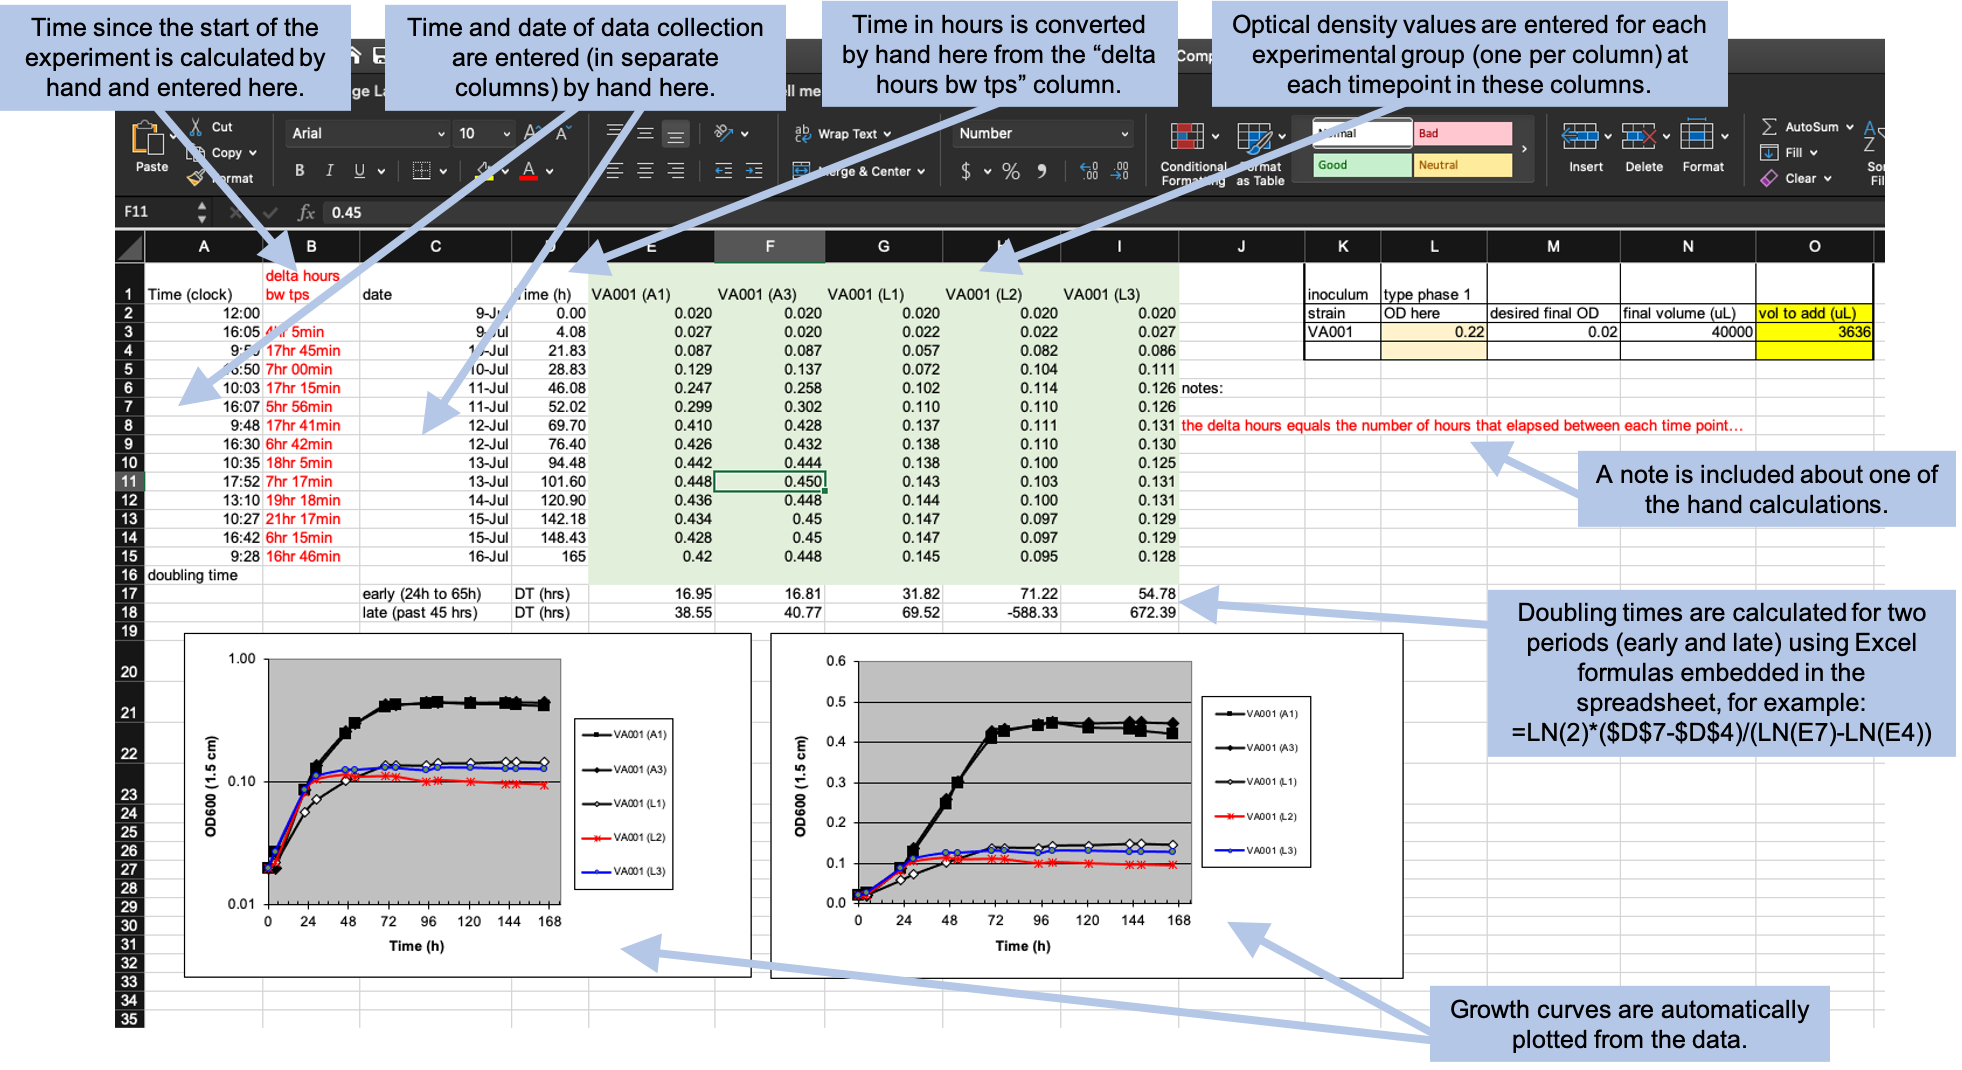
\includegraphics[width=\textwidth]{figures/growth_curve_example} \caption[Example of an Excel spreadsheet used to record and analyze data for a laboratory experiment]{Example of an Excel spreadsheet used to record and analyze data for a laboratory experiment. Annotations highlight where data is entered by hand, where calculations are done by hand, and where embedded Excel formulas are used. The figures are created automatically using values in a specified column.}\label{fig:growthexcel2}
\end{figure*}

In the previous module, we described features that make this template ``untidy''
and potentially problematic to include in a larger pipeline of reproducible
research. In the next few sections of this module, we'll walk step-by-step
through changes that you could make to make this template tidier. We'll finish
the module by showing how you could then easily design a further step of the
analysis pipeline to visualize and analyze the collected data, so that the
advantages of real-time plotting from the more complex spreadsheet are not
missed when moving to a tidier template.

\hypertarget{limiting-the-template-to-the-collection-of-data}{%
\subsection{Limiting the template to the collection of data}\label{limiting-the-template-to-the-collection-of-data}}

The example template (Figure \ref{fig:growthexcel2}) includes a number of
``extra'' elements beyond simple data collection---all the elements outside rows
1--15 of columns A--I. Outside this area of the original spread, there are a
number of extra elements, including plots that visualize the data, summaries
generated based on the data (rows 16--18, for example), notes about the data,
and even a macro (top right) that wasn't involved in data collection but instead
was used by the researcher to calculate the initial volume of inoculum to
include in each test tube. None of these ``extras'' can be easily read into a
statistical program like R or Python---at best, they will be ignored by the program.
They can even complicate reading in the cells with measurements (rows
1--15 of columns A--I), as most statistical programs will try to read in all the
non-empty cells of a spreadsheet unless directed otherwise.

A good starting point, then, would be to start designing a tidy data collection
template for this experiment by extracting only the content from the box in
Figure \ref{fig:extractraw}. This would result in a template that looks like
Figure \ref{fig:step1}.

\begin{figure*}
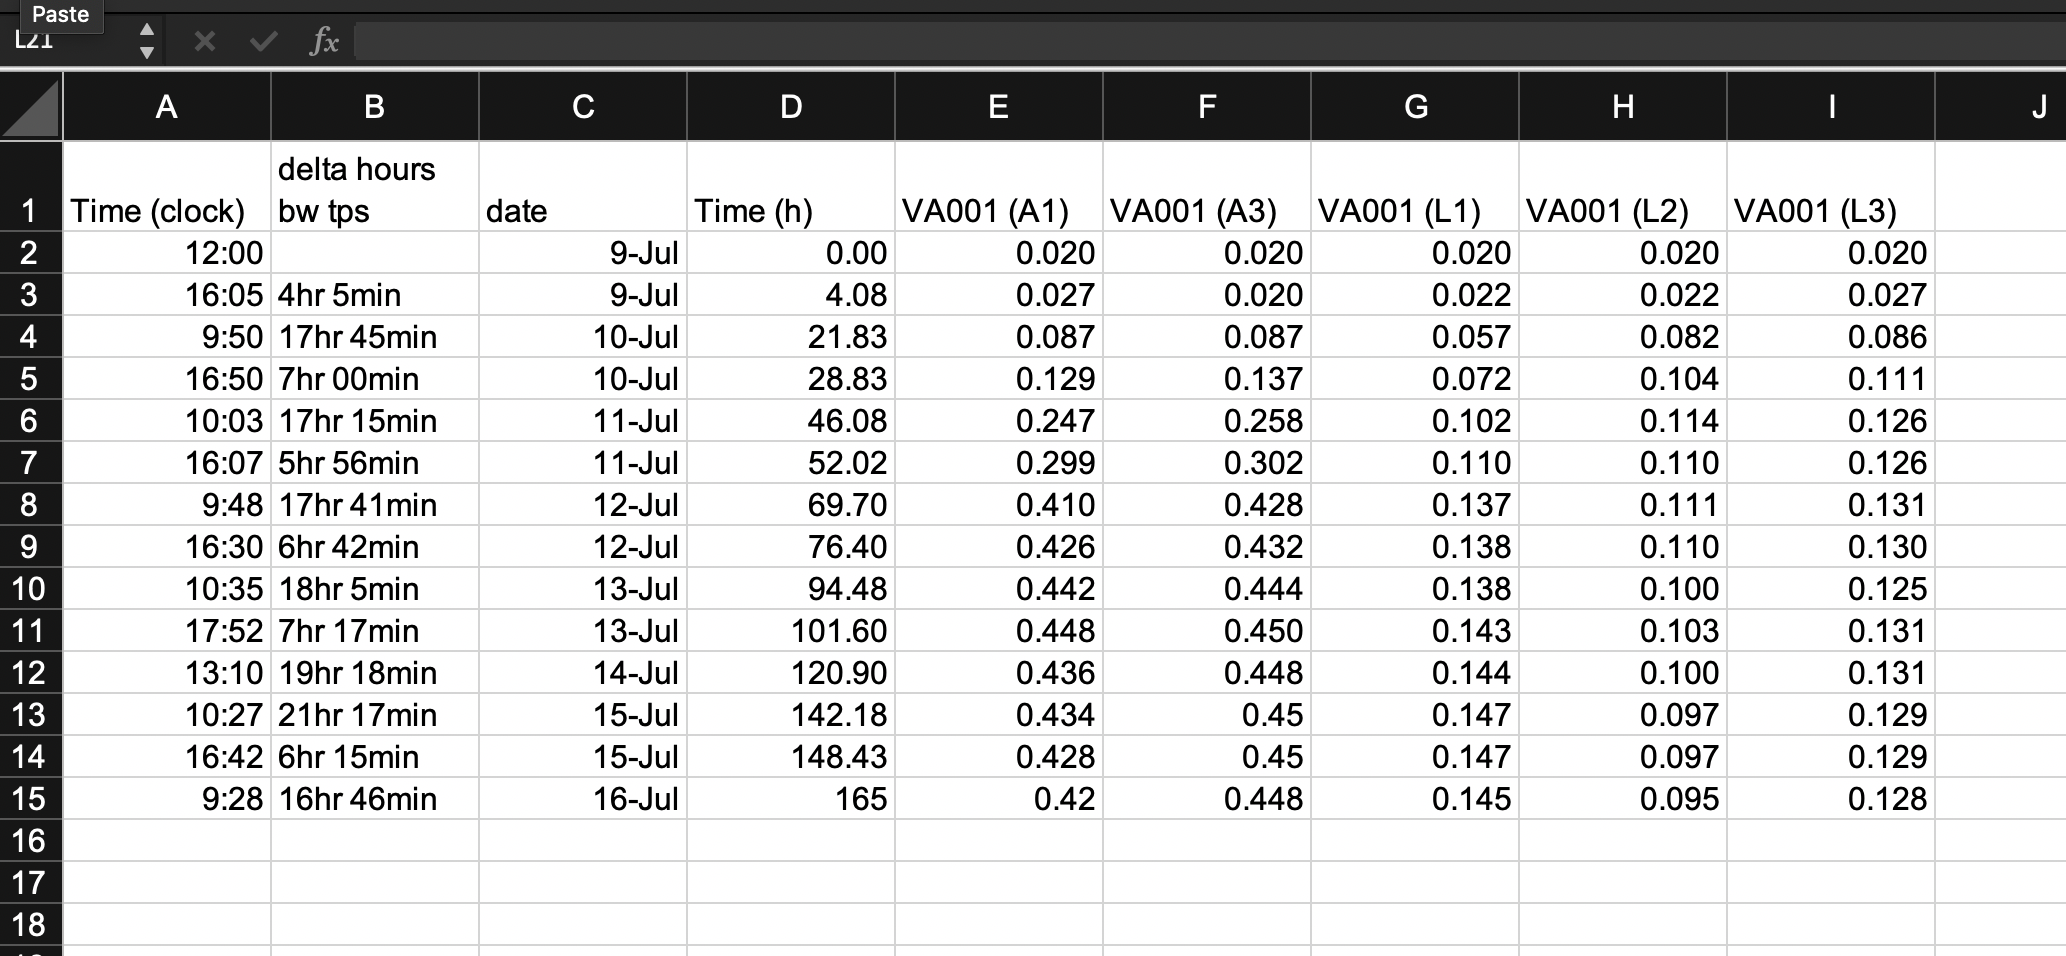
\includegraphics[width=\textwidth]{figures/growth_curve_step1} \caption[First step in designing a tidy data collection template for the example project]{First step in designing a tidy data collection template for the example project. A template has been created that focuses only on the raw data, removing all extra elements like plots, notes, macros, and summaries.}\label{fig:step1}
\end{figure*}

Notice that we've also removed any of the color formatting from the spreadsheet. It is fine to
keep color in the spreadsheet if it will help the research to find the right spot to record data
while working in the laboratory, but you should make sure that you're not using it to encode
information about the data---all color formatting will be ignored when the data are read by a
statistical program like R.

While the template shown in Figure \ref{fig:step1} has removed a lot of the calculated values from the
original template, it has not removed all of them. Two of the columns are still values that were
determined by calculation after the original data were collected. Column B and column D both provide
measures of the length of time since the start of the experiment, and both are calculated by
comparing a measurement time to the time at the start of the experiment.

The time since the start of the experiment can easily be calculated later in the analysis pipeline,
once you read the data into a statistical program like R. By delaying this step, you can both
simplify the data collection template (requiring fewer columns for the research in the laboratory
to fill out) and also avoid the chance for mistakes, which could occur both in the hand calculations
of these values and in data entry, when the researcher enters the results of the calculations in the
spreadsheet cell. Figure \ref{fig:step2} shows a new version of the template, where these calculated
columns have been removed. This template is now restricted to only data points originally collected
in the course of the experiment, and has removed all elements that are based on calculations or other
derivatives of those original, raw data points.

\begin{figure}
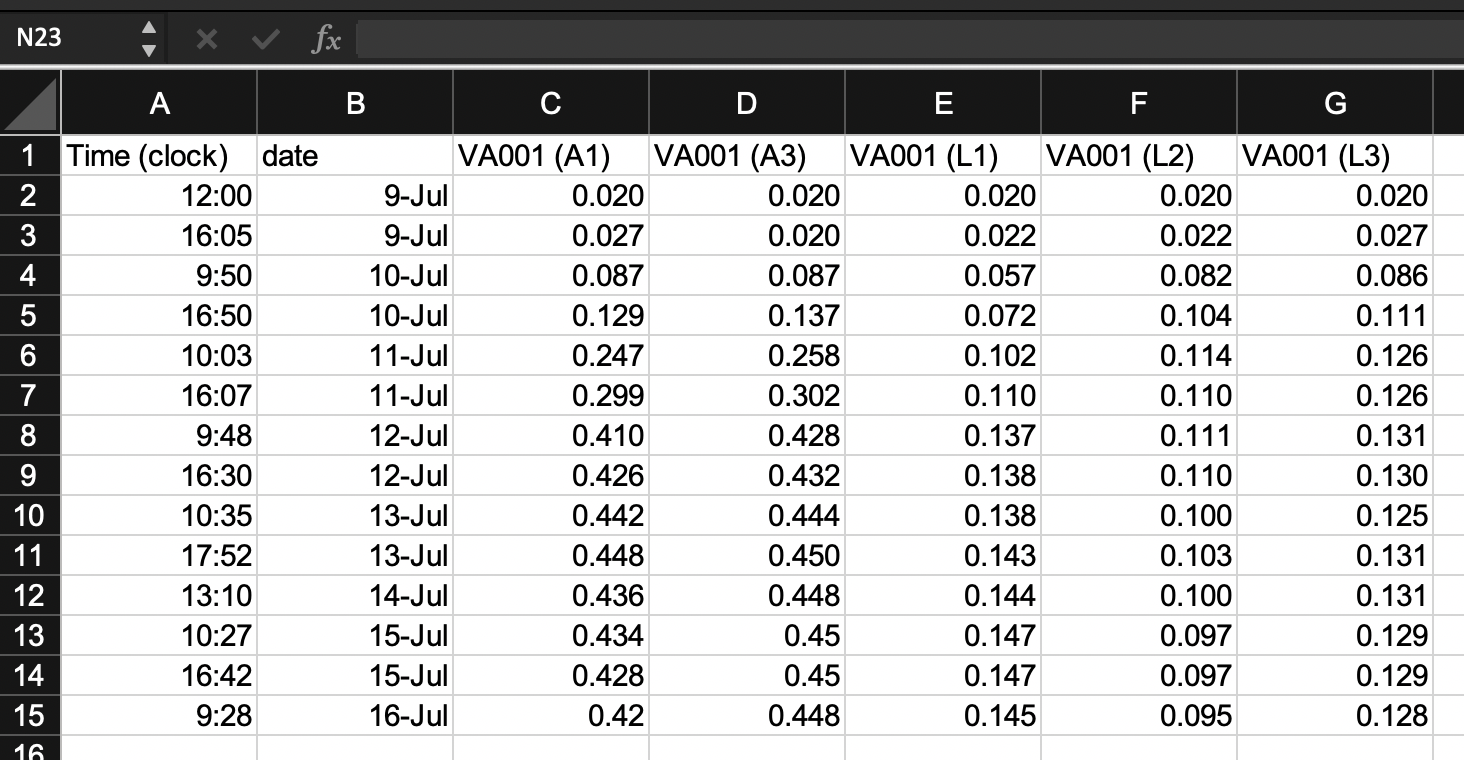
\includegraphics[width=\textwidth]{figures/growth_curve_step2} \caption[Second step in designing a tidy data collection template for the example project]{Second step in designing a tidy data collection template for the example project. This template started from the previous one, but removed columns that were hand-calculated and then entered by the researcher in the previous template. This version has removed all calculated values on the template, limiting it to only the original recorded values required for the experiment.}\label{fig:step2}
\end{figure}

\hypertarget{making-sensible-choices-about-rows-and-columns}{%
\subsection{Making sensible choices about rows and columns}\label{making-sensible-choices-about-rows-and-columns}}

The second principle is to \textbf{make sensible choices when dividing data collection
into rows and columns}. There are many different ways that you could spread the
data collection into rows and columns, and in this step, you can consider which
method would meet a reasonable balance between making the template easy for the
researcher in the laboratory to use to record data and also making the resulting
data file easy to incorporate in a reproducible data analysis pipeline.

For the example experiment, Figure \ref{fig:extractraw} shows three examples
that we can consider for how to arrange data collection across rows and columns.
All three build on the changes we made in the earlier step of ``tidying'' the template,
which resulted in the template shown in Figure \ref{fig:step2}.

\begin{figure*}
\includegraphics[width=\textwidth]{figures/growth_curve_column_options} \caption[Examples of ways that data collection could be divided into rows and columns in the example template]{Examples of ways that data collection could be divided into rows and columns in the example template. Panel A shows an example where date and time are recorded in different columns. Panel B is similar to Panel A, but in this case, date and time are recorded in a single column. Panel C shows a classically 'tidy' data format, where each measurement date-time is repeated for each of the five test tubes, and columns give the test tube ID and absorbance measurement at that time for that tube (only part of the data is shown for this format, while remaining rows are off the page). While Panel C provides the 'tidiest' format, it may have some practical constraints when used in a laboratory setting. For example, it would require more data entry during data collection (since date-time is entered five times at each measurement time), and its long format prevent it all from being seen at once without scrolling on a computer screen.}\label{fig:columnoptions}
\end{figure*}

Panel A (an exact repeat of the template shown in Figure \ref{fig:step2}) shows
an example where date and time are recorded in different columns. Panel B is
similar to Panel A, but in this case, date and time are recorded in a single
column. Panel C shows a classically ``tidy'' data format, where each measurement's
date-time is repeated for each of the five test tubes, and columns give the test
tube ID and absorbance measurement at that time for that tube (only part of the
data is shown for this format, while remaining rows are off the page).

In this example, the template that may be the most reasonable is the one shown
in Panel B. While Panel C provides the ``tidiest'' format, it has some practical
constraints when used in a laboratory setting. For example, it would require
more data entry during data collection (since date-time is entered five times at
each measurement time), and its long format prevent it all from being seen at
once without scrolling on a computer screen. When comparing Panels A and B, the
template in Panel B has an advantage. The information on date and time are
useful together, but not individually. For example, to calculate the time since
the start of the experiment, you cannot just calculate the difference in dates
or just the difference in times, but instead must consider both the date and
time of the measurement in comparison to the date and time of the start of the
experiment. As a result, at some point in the data analysis pipeline, you'll
need to combine information about the date and the time to make use of the two
elements. While this combination of two columns can be easily done within a
statistical program like R, it can also be directly designed into the original
template for collecting the data. Therefore, unless there is a practical reason
why it would be easier for the researcher to enter date and time separately, the
template shown in Panel B is preferable to that shown in Panel A in terms of
allowing for the ``tidy'' collection of research data into a file that is easy to
include in a reproducible pipeline. Figure \ref{fig:step3} shows the template
design at this stage in the process of tidying it, highlighting the column that
combines date and time elements in a single column. In this version of the
template, we've also been careful about how date and time are recorded, a
consideration that we'll discuss more in the next section.

\begin{figure*}
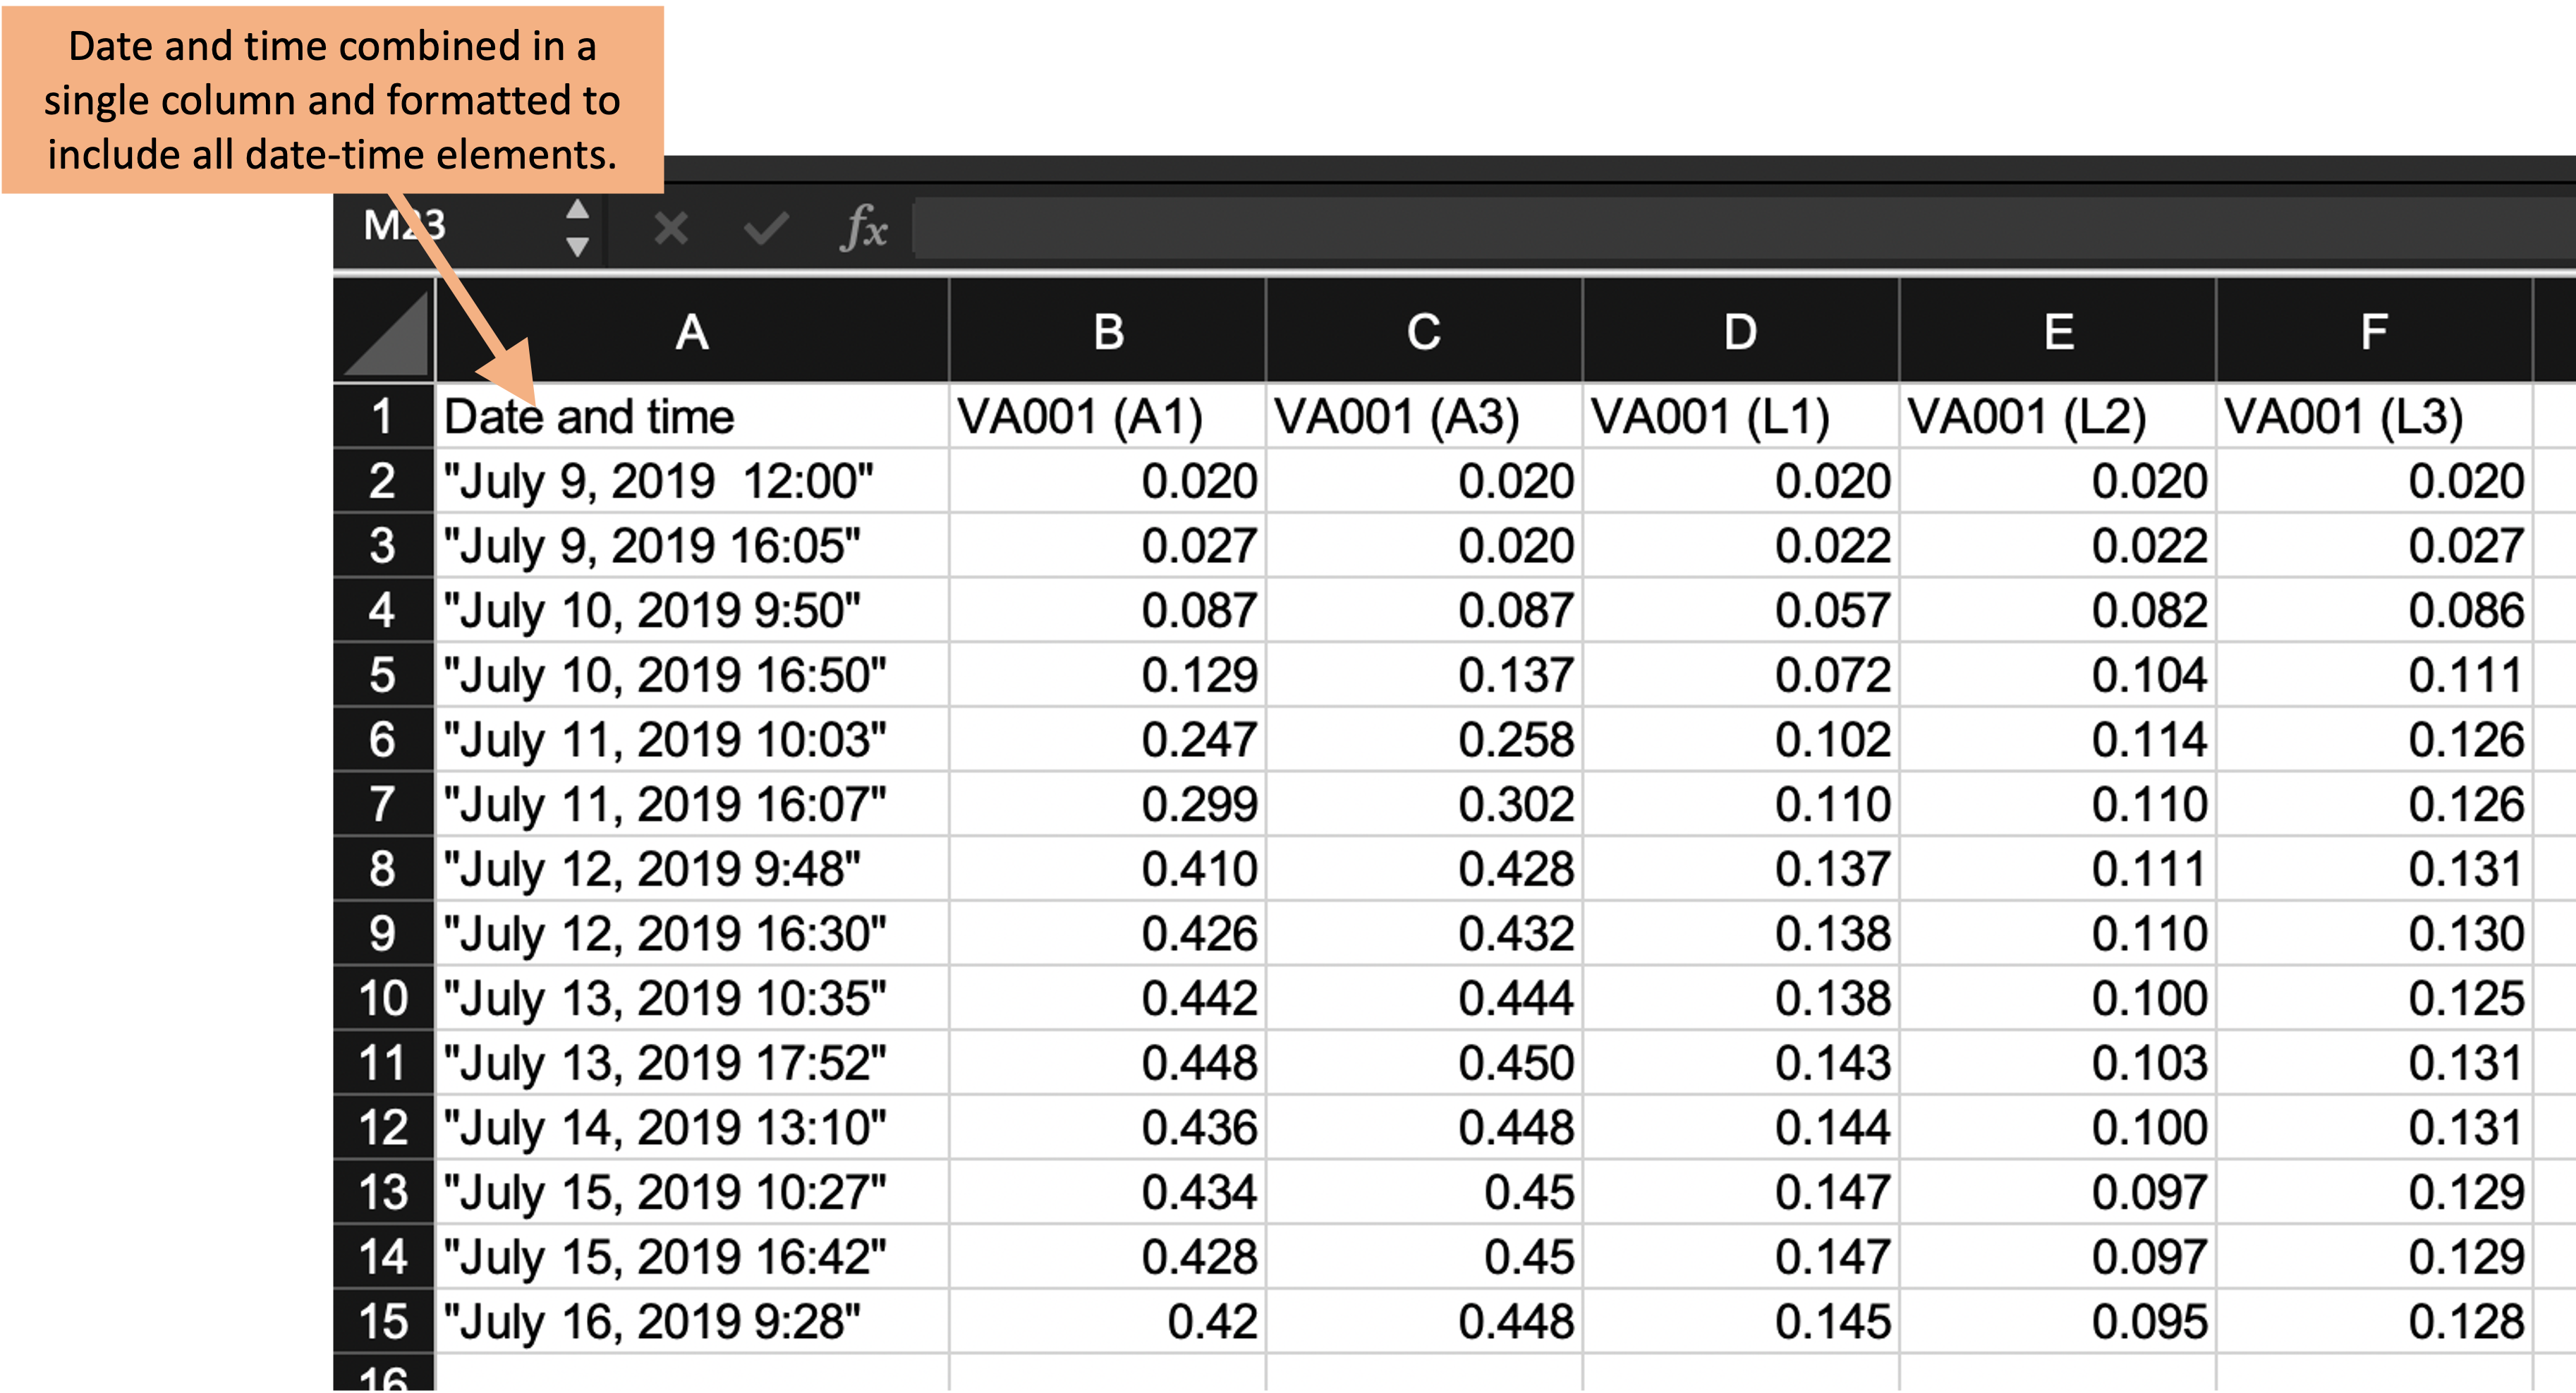
\includegraphics[width=\textwidth]{figures/growth_curve_step3} \caption[Third step in designing a tidy data collection template for the example project]{Third step in designing a tidy data collection template for the example project. This template started from the previous one, but combined collection of the date and time of the measurement into a single column and revised the format to include all date elements and to prevent automatic conversion by the spreadsheet program.}\label{fig:step3}
\end{figure*}

\hypertarget{avoiding-problematic-characters-or-formatting}{%
\subsection{Avoiding problematic characters or formatting}\label{avoiding-problematic-characters-or-formatting}}

The third principle is to \textbf{avoid characters or formatting that will make it
hard for a computer program to process the data}. There are a number of special
characters and formatting conventions that can be hard for a statistical program to
handle. In the example template shown in Figure \ref{fig:step3}, for example,
the column names include spaces (for example, in ``Date and time''), as well as
parenthese (for example, in ``VA 001 (A1)''). While most statistical programs have
tools that allow you to handle and convert these characters once the data are
read in, it's even simpler to use simpler column names in the original data collection
template, and this will save some extra coding further along in the analysis pipeline.
Two general rules for creating easy-to-use column names in a data collection template
are: (1) start each column name with a letter and (2) for the rest of the column
name, use only letters, numbers, or the underscore character ("\_``). For example,''aerated1" would work well, but ``1--aerated'' would not.

Within the cell values below the column names, there is more flexibility. For example,
if you have a column that gives the IDs of different samples, it would be fine to include
spaces and other characters in those IDs. There are a few exceptions, however. A big one
is with values that record dates or date-time combinations. First, it is important to include
all elements of the date (or date and time, if both are recorded). For example, the year
should be included in the recorded date, even if the experiment only took a few days.
This is because statistical programs have excellent functions for working with data that
are dates or date-times, but to take advantage of these, the data must be converted into
a special class in the program, and conversion to that class requires specific elements
(for example, a date must include the year, month, and day of month). Second, it is
useful to avoid recording dates and date-times in a way that results in a spreadsheet
program automatically converting them. Surrounding the information about a date in
quotation marks when entering it (as shown in Figure \ref{fig:step3}) can avoid this.
Finally, consider using a format to record the date that is unambiguous and so less likely
to have recording errors. Dates, for example, are sometimes recorded using only numbers---for
example, the first date of ``July 9, 2019'' in the example data could be recorded as
``7/9/2019'' or ``7/9/19'', to be even more concise. However, this format has some ambiguity.
It can be unclear if this refers to July 9 or to September 7, both of which could be
written as ``7/9''. For the version that uses two digits for the year, it can be unclear
if the date is for 2019 or 1919 (or any other century). Using the format ``July 9, 2019'',
as done in the latest version of the sample template, avoids this potential ambiguity.

Figure \ref{fig:growthsimple2} shows the template for the example experiment after the
column names have been revised to avoid any problematic characters. This template is now in
a very useful format for a reproducible research pipeline---the data collected using this
template can be very easily read into and processed using further statistical programs like
R or Python.

\begin{figure}
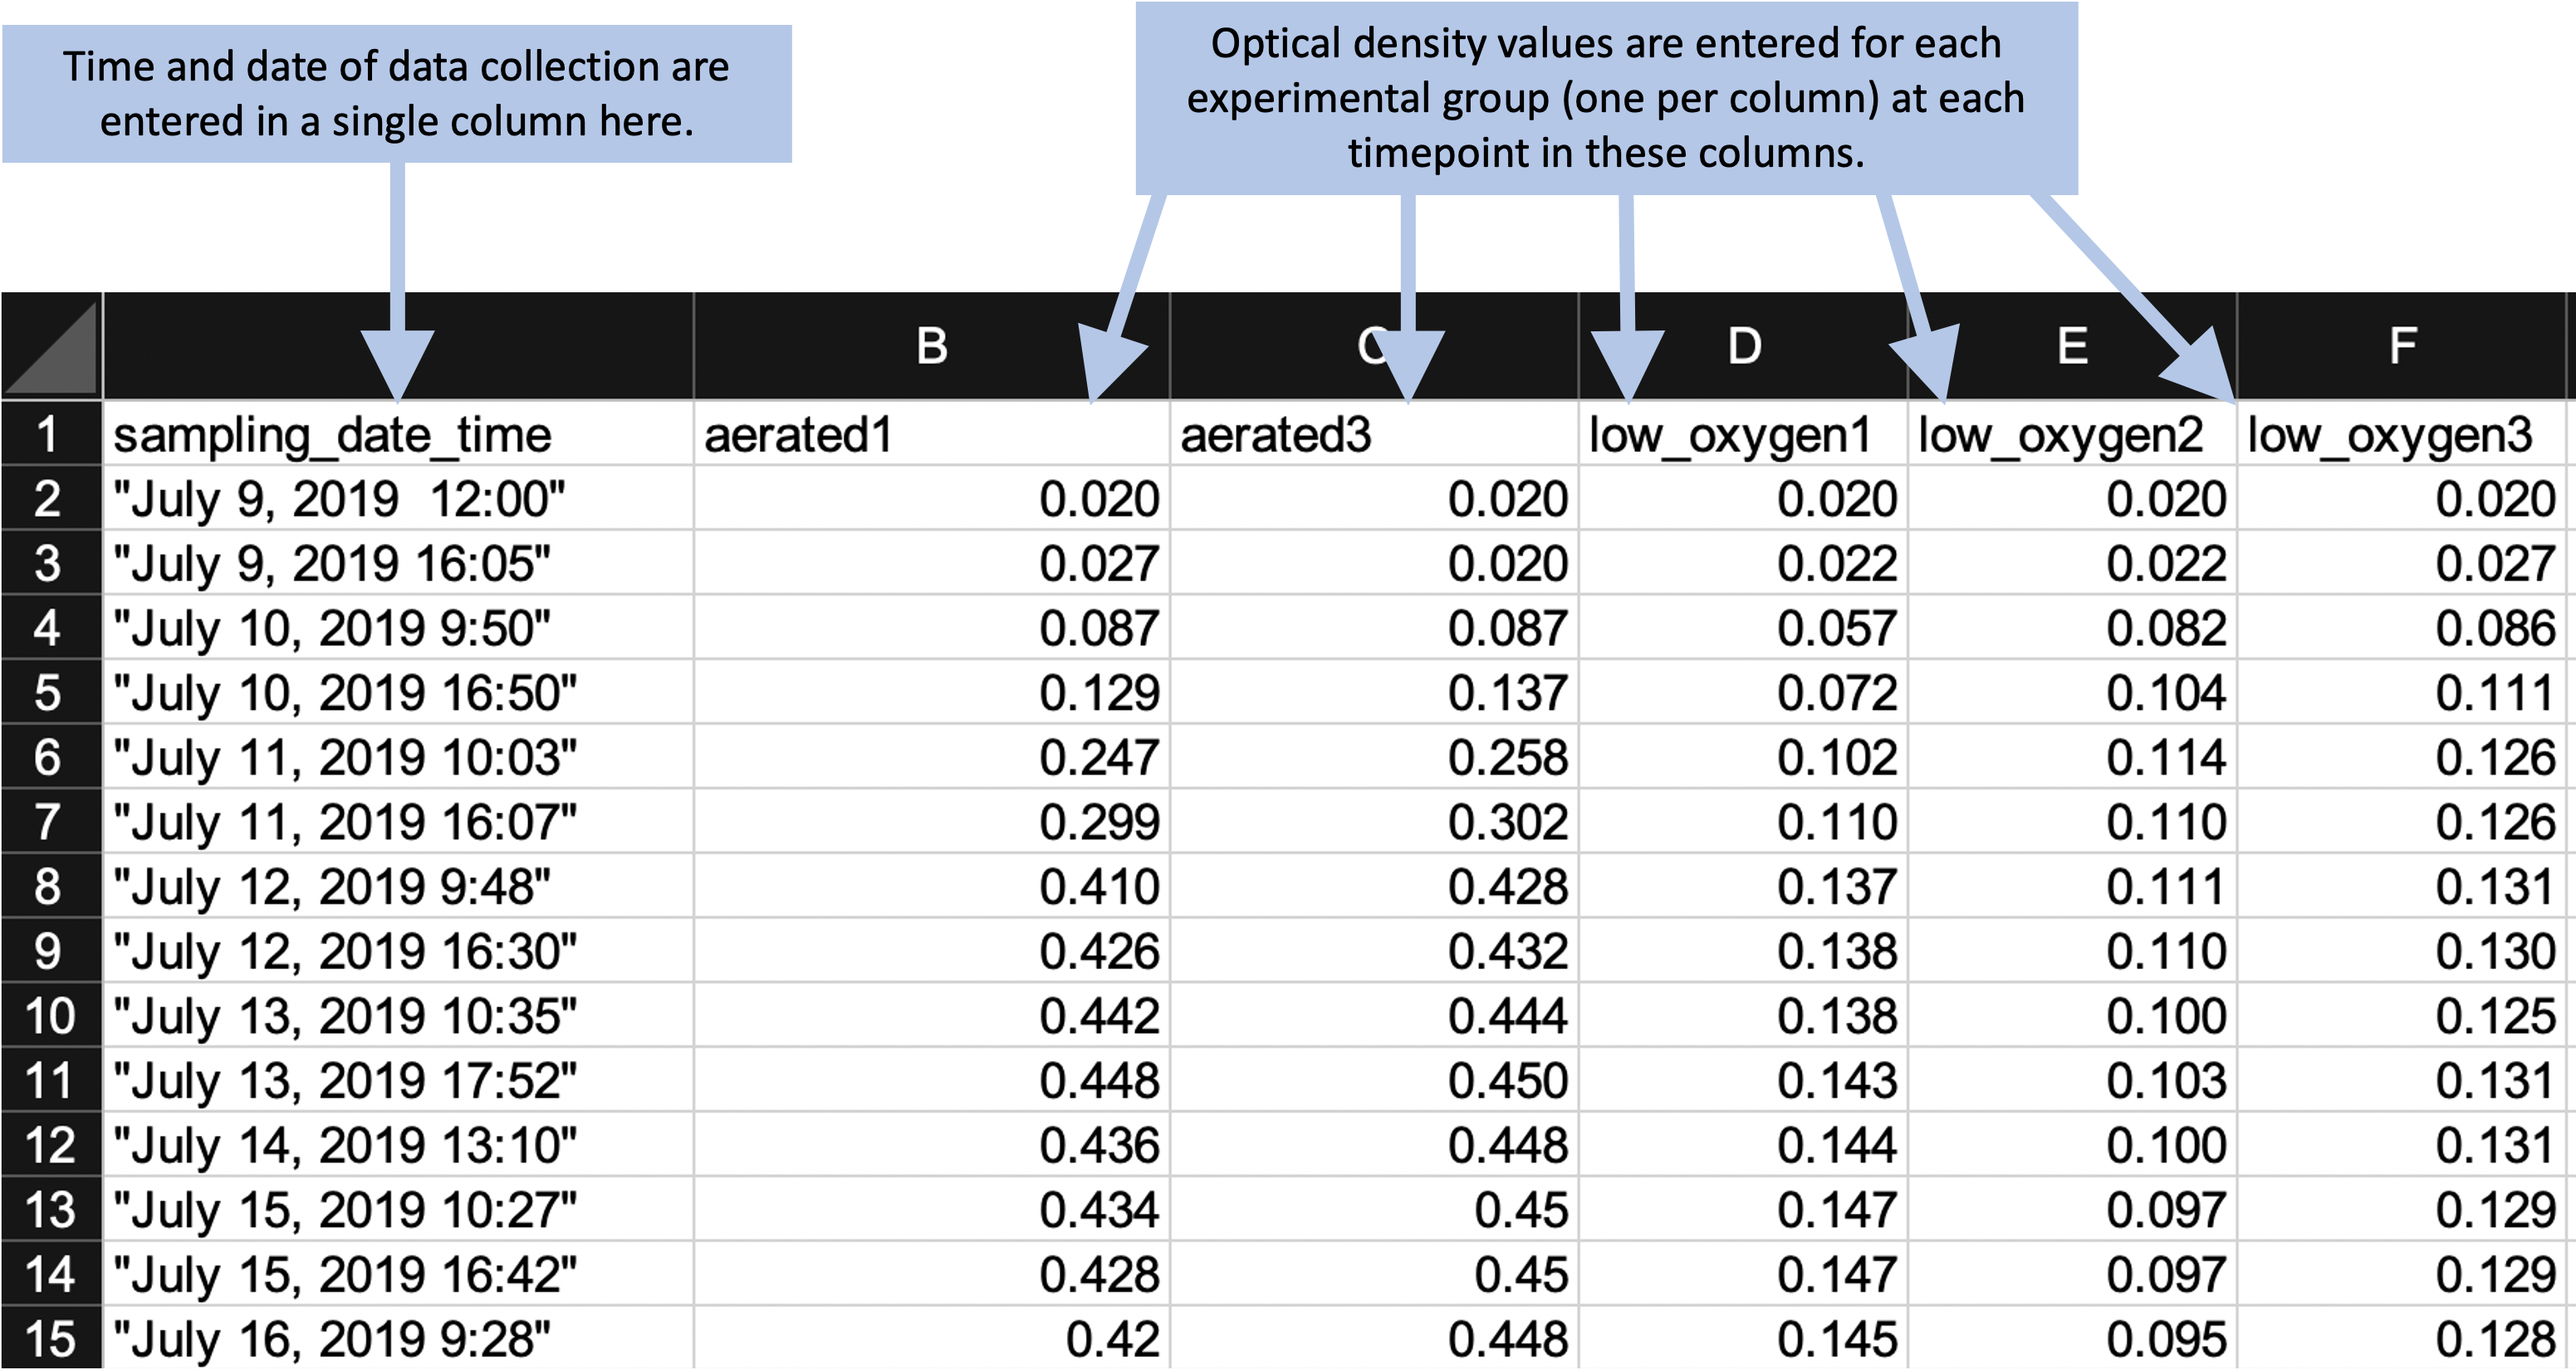
\includegraphics[width=\textwidth]{figures/growth_curve_simple} \caption[Example of an simpler format that can be used to record and analyze data for the same laboratory experiment as the previous figure]{Example of an simpler format that can be used to record and analyze data for the same laboratory experiment as the previous figure. Annotations highlight where data is entered by hand. No calculations are conducted or figures created---these are all done later, using a code script.}\label{fig:growthsimple2}
\end{figure}

\hypertarget{moving-further-data-analysis-to-later-in-the-pipeline}{%
\subsection{Moving further data analysis to later in the pipeline}\label{moving-further-data-analysis-to-later-in-the-pipeline}}

\begin{figure*}
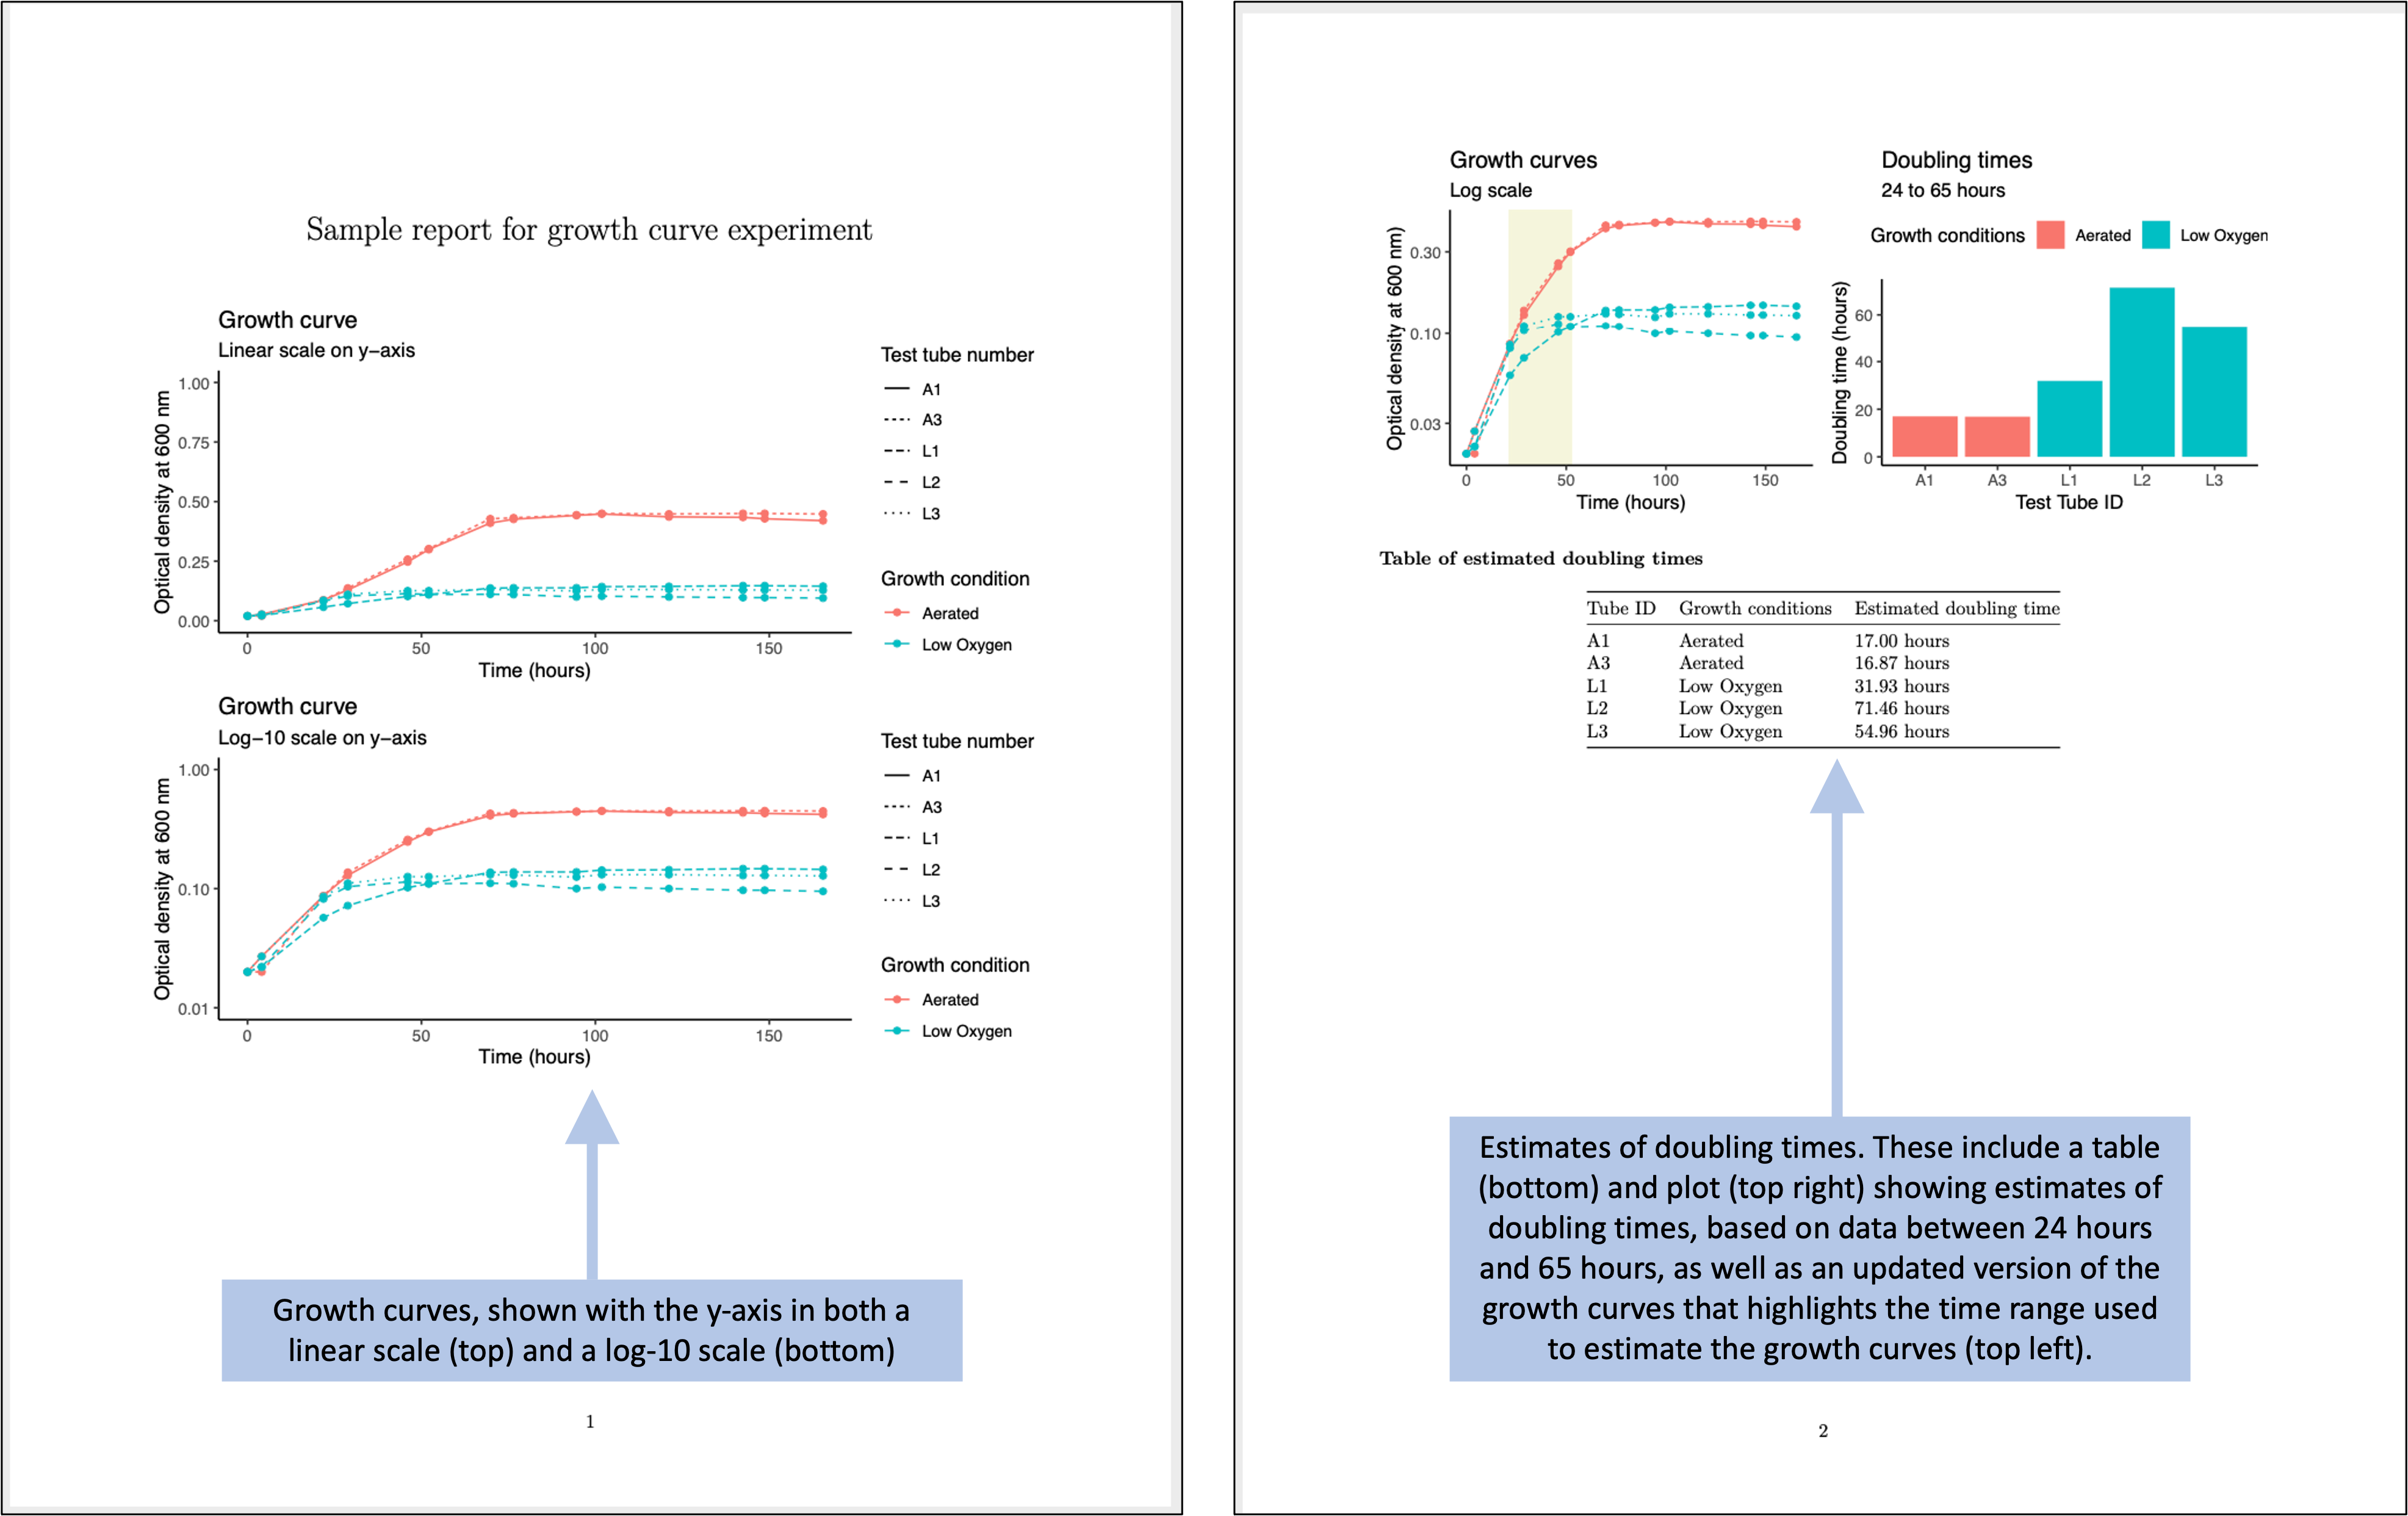
\includegraphics[width=\textwidth]{figures/growth_curve_report} \caption[Examples of an automated report that can be created to quickly generate summaries and estimates of the data collected in the simplified data collection template for the example experiment]{Examples of an automated report that can be created to quickly generate summaries and estimates of the data collected in the simplified data collection template for the example experiment.}\label{fig:growthreport2}
\end{figure*}

\begin{center}\rule{0.5\linewidth}{0.5pt}\end{center}

\textbf{Older text}

\hypertarget{exampledata-on-rate-of-bacterial-growth-1}{%
\subsection{Example---Data on rate of bacterial growth}\label{exampledata-on-rate-of-bacterial-growth-1}}

The first set of data are from a study on the growth of \emph{Mycobacterium
tuberculosis}. The goal of this study was to compare growth yield and doubling
time of \emph{Mycobacterium tuberculosis} grown in rich medium under two assay
conditions. One set of cultures were grown in tubes with a low culture volume
relative to a large air head space to allow free oxygen exchange. A second set
of cultures were grown in tubes filled to near capacity, resulting in limited
air head space which has been shown elsewhere to limit oxygen availability over
time. The caps on both sets of cultures were sealed to restrict air exchange
during the study.

Some background information is helpful in understanding these example data,
especially if you have not conducted this type of experiment. The increase in
the cell size and cell mass during the development of an organism is termed
growth. It is the unique characteristics of all organisms. The organism must
require certain basic parameters for their energy generation and cellular
biosynthesis. The growth of the organism is affected by both physical and
nutritional factors. There are multiple methods by which growth can be measured,
but the use of closed tissue culture tubes and a spectrophotometer to track
increases in optical density (absorbance at 600 nm) over time offers several
advantages: 1) it is less subject to technical error and contamination, 2) read
out is fast and simple, 3) growth as measure by increased absorbance (turbidity)
is directly proportional to increases in cell mass. There are four distinct
phases of bacterial growth. Lag phase, log (exponential phase), stationary
phase, death phase. From these data, bacterial generation times (doubling time)
during the exponential growth phase can be calculated.

\[
\mbox{Doubling time} = \frac{log(2)(t_1 - t_2)}{log(OD_{t_1} - log(OD_{t_2}))}
\]
where \(t_1\) and \(t_2\) are two time points and \(OD_{t_1}\) and \(OD_{t_2}\) are the
optical densities at the two time points (all \(log\)s are natural in this case).

An excel-based workbook (Figure \ref{fig:growthexcel2}) was created to allow the
student performing the work to (1) calculate the amount of initial inoculum
(cell culture) to add to each tube to begin the study, (2) record the raw data
absorbance measurements, (3) graph the data on both a log and linear scale, and
(4) calculate doubling time in two phases of growth using the equation listed
above. Columns were added to allow the student to track the time (column A), the
difference in time (hours) between each time point in which data were collected
(column B), the date on which data were gathered (column C), and the time in
hours for each data point from the start of the study for graphing purposes
(column D). Absorbance data for each sampling timepoint were listed in Columns
E-F (high oxygen conditions; VA001 A1, A3) or columns G-I (limited oxygen
conditions; VA001 L1, L2, L3).

What the researchers found appealing about the format of this Excel sheet was
the ease with which the student could accomplish the study goals. They also
cited transparency of the raw data and ease with which additional sampling data
points could be added. The data being graphed in real time and the inclusion of
a simple macro to calculate doubling time, allowed the student to see tangible
differences between the two assay conditions. This was also somewhat problematic
as the equation to calculate doubling time was based on anchored time points
built into the original spreadsheet resulting in two different results that were
not properly linked to the correct data time points.

Data that are saved in a format like that shown in Figure \ref{fig:growthexcel2},
however, are hard to read in for a statistical program like R, Perl, or Python.
In this format, the raw data (the time points each observation was collected and
the optical density for the sample at that time point) form only part of the
spreadsheet. The spreadsheet also includes notes, automated figures, and
cells where an embedded formula runs calculations behind the scenes.

Instead of this format, we can design a simpler format to collect the data. We'll
remove all figures and calculations, and instead save those to perform in a
code script. Figure \ref{fig:growthsimple} shows an example of a simpler
format for collecting the same data. In this case, all the ``extras'' have been
stripped out---this only has spaces for recording times points and the observed
optical density at those time points. In later chapters, we'll show how a code
script can be used to input these data into R and then perform calculations
and create figures. By separating out the steps of data recording from
data analysis, you can ensure that all steps of analysis are clearly spelled
out (and can be easily reproduced with other similar data) through a code
script. Note that you can still collect the data in this simpler format using
a spreadsheet program, if you'd like---Figure \ref{fig:growthsimple2} shows
the data collection set up to be recorded in a spreadsheet program, for example.
Within the spreadsheet, you can choose to save the data in a plain text format
(a csv {[}comma-separated value{]} file, for example).

In this new data collection format, the data are not completely ``tidy''. This is because
there is still some information included in the column names that we might want to use
for analysis and plotting---namely, the different experimental group names (e.g.,
``aerated1'', ``low\_oxygen1''). However, there is a balance in creating data collection
spreadsheets. They should be in a format that is easy to read into an interactive
programming environment like R, as well as in a format that will be easy to convert
to a truly ``tidy'' format once they are read in. However, it's okay to balance these
needs with aims to make the data collection spreadsheet easy for a researcher to use.

The example shown in Figure \ref{fig:growthsimple2} is designed to be easy to use
when collecting data. All data points for a single collection time are grouped together
on a single row. When a researchers collects data for one time point, he or she can
easy confirm visually that all the experimental groups have been measured for that
time point. This format still makes it easy to read the data into an interactive
programming environment, however, since they are in a clear two-dimensional format,
with column names in the first row and values in the remaining rows. The removal of
extraneous elements---like embedded formulas, the results of hand calculations or
automated calculations, and annotations through notes or colored highlighting---remove
barriers when reading the data into more sophisticated software. Once the data are
read into R, there can be converted into a truly tidy data format with just a few
command calls.

The following code shows an example of how easy it is to read data into R in the simplified
format shown in Figure \ref{fig:growthsimple2}. It also shows how a few lines of code
can then be used to convert the data into a truly ``tidy'' format, and how easily
sophisticated plots can then be made with the data.

\begin{Shaded}
\begin{Highlighting}[]
\FunctionTok{library}\NormalTok{(}\StringTok{"tidyverse"}\NormalTok{)}
\FunctionTok{library}\NormalTok{(}\StringTok{"readxl"}\NormalTok{)}

\CommentTok{\# Read data into R from the simplified data collection template}
\NormalTok{growth\_curve }\OtherTok{\textless{}{-}} \FunctionTok{read\_excel}\NormalTok{(}\StringTok{"data/growth\_curve\_data\_in\_excel (1)/growth curve data\_GR.xls"}\NormalTok{, }
                           \AttributeTok{sheet =} \StringTok{"simplified\_template"}\NormalTok{)}

\CommentTok{\# Example of data}
\NormalTok{growth\_curve}
\end{Highlighting}
\end{Shaded}

\begin{verbatim}
## # A tibble: 14 x 6
##    sampling_date_time  aerated1 aerated3 low_oxygen1 low_oxygen2 low_oxygen3
##    <dttm>                 <dbl>    <dbl>       <dbl>       <dbl>       <dbl>
##  1 2019-07-09 12:00:00    0.02     0.02        0.02        0.02        0.02 
##  2 2019-07-09 16:05:00    0.027    0.02        0.022       0.022       0.027
##  3 2019-07-10 09:50:00    0.087    0.087       0.057       0.082       0.086
##  4 2019-07-10 16:50:00    0.129    0.137       0.072       0.104       0.111
##  5 2019-07-11 10:03:00    0.247    0.258       0.102       0.114       0.126
##  6 2019-07-11 16:07:00    0.299    0.302       0.11        0.11        0.126
##  7 2019-07-12 09:48:00    0.41     0.428       0.137       0.111       0.131
##  8 2019-07-12 16:30:00    0.426    0.432       0.138       0.11        0.13 
##  9 2019-07-13 10:35:00    0.442    0.444       0.138       0.1         0.125
## 10 2019-07-13 17:52:00    0.448    0.45        0.143       0.103       0.131
## 11 2019-07-14 13:10:00    0.436    0.448       0.144       0.1         0.131
## 12 2019-07-15 10:27:00    0.434    0.45        0.147       0.097       0.129
## 13 2019-07-15 16:42:00    0.428    0.45        0.147       0.097       0.129
## 14 2019-07-16 09:28:00    0.42     0.448       0.145       0.095       0.128
\end{verbatim}

\begin{Shaded}
\begin{Highlighting}[]
\CommentTok{\# Convert to a fully tidy format}
\NormalTok{growth\_curve }\OtherTok{\textless{}{-}}\NormalTok{ growth\_curve }\SpecialCharTok{\%\textgreater{}\%} 
  \FunctionTok{pivot\_longer}\NormalTok{(}\SpecialCharTok{{-}}\NormalTok{sampling\_date\_time, }
               \AttributeTok{names\_to =} \StringTok{"experimental\_group"}\NormalTok{, }
               \AttributeTok{values\_to =} \StringTok{"optical\_density"}\NormalTok{)}

\CommentTok{\# How the data look after this transformation}
\NormalTok{growth\_curve}
\end{Highlighting}
\end{Shaded}

\begin{verbatim}
## # A tibble: 70 x 3
##    sampling_date_time  experimental_group optical_density
##    <dttm>              <chr>                        <dbl>
##  1 2019-07-09 12:00:00 aerated1                     0.02 
##  2 2019-07-09 12:00:00 aerated3                     0.02 
##  3 2019-07-09 12:00:00 low_oxygen1                  0.02 
##  4 2019-07-09 12:00:00 low_oxygen2                  0.02 
##  5 2019-07-09 12:00:00 low_oxygen3                  0.02 
##  6 2019-07-09 16:05:00 aerated1                     0.027
##  7 2019-07-09 16:05:00 aerated3                     0.02 
##  8 2019-07-09 16:05:00 low_oxygen1                  0.022
##  9 2019-07-09 16:05:00 low_oxygen2                  0.022
## 10 2019-07-09 16:05:00 low_oxygen3                  0.027
## # ... with 60 more rows
\end{verbatim}

\begin{Shaded}
\begin{Highlighting}[]
\CommentTok{\# Example of how easily sophisticated plots can be created with data in this format}
\NormalTok{growth\_curve }\SpecialCharTok{\%\textgreater{}\%} 
  \FunctionTok{ggplot}\NormalTok{(}\FunctionTok{aes}\NormalTok{(}\AttributeTok{x =}\NormalTok{ sampling\_date\_time, }\AttributeTok{y =}\NormalTok{ optical\_density)) }\SpecialCharTok{+} 
  \FunctionTok{geom\_line}\NormalTok{() }\SpecialCharTok{+} 
  \FunctionTok{facet\_wrap}\NormalTok{(}\SpecialCharTok{\textasciitilde{}}\NormalTok{ experimental\_group)}
\end{Highlighting}
\end{Shaded}

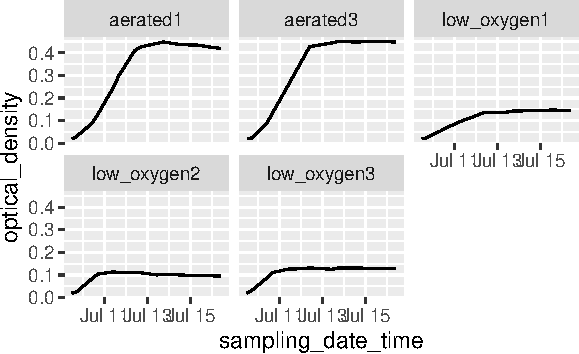
\includegraphics{improve_repro_files/figure-latex/unnamed-chunk-3-1}
In later chapters, we'll discuss R's ``tidyverse'', a collection of tools within R
that facilitate analyzing and visualizing data once they've been read into R. Here, we
only aim to give an example of how little R code is needed to create useful output from
the data, with the only requirement for gaining this power being that the data need to
be collected in a format that is ``tidy'' or close enough to easily read into R.

\hypertarget{exampledata-on-bacteria-colony-forming-units}{%
\subsection{Example---Data on bacteria colony forming units}\label{exampledata-on-bacteria-colony-forming-units}}

\hypertarget{exampledata-from-multiple-related-experiments}{%
\subsection{Example---Data from multiple related experiments}\label{exampledata-from-multiple-related-experiments}}

\hypertarget{issues-with-these-data-sets}{%
\subsection{Issues with these data sets}\label{issues-with-these-data-sets}}

\begin{enumerate}
\def\labelenumi{\arabic{enumi}.}
\tightlist
\item
  Issues related to using a spread sheet program

  \begin{itemize}
  \tightlist
  \item
    Embedded macros
  \item
    Use of color to encode information
  \end{itemize}
\item
  Issues related to non-structured / non-two-dimensional data

  \begin{itemize}
  \tightlist
  \item
    Added summary row
  \item
    Multiple tables in one sheet
  \item
    One cell value is meant to represent values for all rows below, until next
    non-missing row
  \end{itemize}
\item
  Issues with data being non-``tidy''
\end{enumerate}

\hypertarget{final-tidy-examples}{%
\subsection{Final ``tidy'' examples}\label{final-tidy-examples}}

\hypertarget{options-for-recording-tidy-data}{%
\subsection{Options for recording tidy data}\label{options-for-recording-tidy-data}}

\textbf{Spreadsheet program.}

\textbf{Spreadsheet-like interface in R.}

\hypertarget{examples-of-how-tidy-data-can-be-easily-analyzed-visualized}{%
\subsection{Examples of how ``tidy'' data can be easily analyzed / visualized}\label{examples-of-how-tidy-data-can-be-easily-analyzed-visualized}}

\hypertarget{discussion-questions-1}{%
\subsection{Discussion questions}\label{discussion-questions-1}}

\hypertarget{module6}{%
\section{Power of using a single structured `Project' directory for storing and tracking research project files}\label{module6}}

To improve the computational reproducibility of a research project, researchers
can use a single `Project' directory to collectively store all research data,
meta-data, pre-processing code, and research products (e.g., paper drafts,
figures). We will explain how this practice improves the reproducibility and
list some of the common components and subdirectories to include in the
structure of a `Project' directory, including subdirectories for raw and
pre-processed experimental data.

\textbf{Objectives.} After this module, the trainee will be able to:

\begin{itemize}
\tightlist
\item
  Describe a `Project' directory, including common components and subdirectories
\item
  List how a single `Project' directory improves reproducibility
\end{itemize}

\hypertarget{organizing-project-files-through-the-file-system}{%
\subsection{Organizing project files through the file system}\label{organizing-project-files-through-the-file-system}}

One of the most amazing parts of how modern computers work is their file
directory systems. {[}More on these.{]}

It is useful to leverage this system to organize all the files related to a
project. These include data files (both ``raw'' data---directly output from
measurement equipment or directly recorded from observations, as well as any
``cleaned'' version of this data, after steps have been taken to preprocess the
data to prepare it for visualization and analysis in papers and reports). These
files also include the files with writing and presentations (posters and slides)
associated with the project, as well as code scripts for preprocessing data,
for conducting data analysis, and for creating and sharing final figures and
tables.

There are a number of advantages to keeping all files related to a single project
inside a dedicated file directory on your computer. First, this provides a clear
and obvious place to search for all project files throughout your work on the
project, including after lulls in activity (for example, while waiting for
reviews from a paper submission). By keeping all project files within a single
directory, you also make it easier to share the collection of files for the
project. There are several reasons you might want to share these files. An
obvious one is that you likely will want to share the project files across members
in your research team, so they can collaborate together on the project. However,
there are also other reasons you'd need to share files, and one that is growing
in popularity is that you may be asked to share files (data, code scripts, etc.)
when you publish a paper describing your results.

When files are all stored in one directory, the directory can be compressed and
shared as an email attachment or through a file sharing platform like Google Drive.
As you learn more tools for reproducibility, you can also share the directory through
some more dynamic platforms, that let all those sharing access continue to change
and contribute to the files in the directory in a way that is tracked and
reversible. In later modules in this book, we will introduce \texttt{git} version control
software and the GitHub platform for sharing files under this type of version
control---this is one example of this more dynamic way of sharing files within
a directory.

\hypertarget{organizing-files-within-a-project-directory}{%
\subsection{Organizing files within a project directory}\label{organizing-files-within-a-project-directory}}

To gain the advantages of directory-based project file organization, all the
files need to be within a single directory, but they don't all have to be within
the same ``level'' in that directory. Instead, you can use subdirectories to
structure and organize these files, while still retaining all the advantages of
directory-based file organization. This will help limit the number of files in
each ``level'' of the directory, so none becomes an overwhelming slew of files of
different types. It can help you navigate the files in the directory, and also
help someone you share the directory with figure out what's in it and where
everything is.

Subdirectory organizations can also, it turns out, be used in clever ways within
code scripts applied to files in the directory. For example, there are functions
in all scripting languages that will list all the files in a specified subdirectory.
If you keep all your raw data files of a certain type (for example, all output from
running flow cytometry for the project) within a single subdirectory, you can
use this type of function with code scripts to list all the files in that directory
and then apply code that you've developed to preprocess or visualize the data
across all those files. This code would continue to work as you added files to that
directory, since it starts by looking in that subdirectory each time it runs and
working with all files there as of that moment.

It is worthwhile to take some time to think about the types of files that are
often generated by your research projects, because there are also big advantages
to creating a standard structure of subdirectories that you can use consistently
across the directories for all the projects in your research program. Of course,
some projects may not include certain files, and some might have a new or unusual
type of file, so you can customize the directory structure to some degree for these
types of cases, but it is still a big advantage to include as many common elements
as possible across all your projects.

For example, you may want to always include a subdirectory called ``raw\_data'', and
consistently call it ``raw\_data'', to store data directly from observations or
directly output from laboratory equipment. You may want to include subdirectories
in that ``raw\_data'' subdirectory for each type of data---maybe a ``cfu'' subdirectory,
for example, with results from plating data to count colony forming units, and
another called ``flow'' for output from a flow cytometer. By using the same structure
and the same subdirectory names, you will find that code scripts are easier to
reuse from one project to another. Again, most scripting languages allow you to
leverage order in how you've arranged your files in the file system, and so using
the same order across different projects lets you repeat and reuse code scripts
more easily from one project to another.

Finally, if you create a clear and clean organization structure for your project
directories, you will find it is much easier to navigate your files in all
directories, and also that new lab members and others you share the directories
with will be able to quickly learn to navigate them. In other areas of science
and engineering, this idea of standardized directory structures has allowed the
development of powerful techniques for open-source software developers to work
together. For example, anyone may create their own extensions to the R
programming language and share these with others through GitHub or several large
repositories. This is coordinated by enforcing a common directory structure on
these extension ``packages''---to create a new package, you must put certain types
of files in certain subdirectories within a project directory. With these
standardized rules of directory structure and content, each of these packages
can interact with the base version of R, since there are functions that can tap
into any of these new packages by assuming where each type of file will be
within the package's directory of files. In a similar way, if you impose a
common directory structure across all the project directories in your research
lab, your collaborators will quickly be able to learn where to find each
element, even in projects they are new to, and you will all be able to write
code that can be easily applied across all project directories, allowing you to
improve reproducibility and comparability across all projects by assuring that
you are conducting the same preprocessing and analysis across all projects (or,
if you are conducting things differently for different projects, that you are
deliberate and aware that you are doing so).

Figure {[}x{]} gives an example of a project directory organization that might make
sense for a immunology research laboratory.

Once you have decided on a structure for your directory, you can create a
template of it---a file directory with all the subdirectories included, but
without any files (or only template files you'd want to use as a starting
point in each project). When you start a new project, you can then just
copy this template and rename it. If you are using R and begin to use
R Project (described in the next section), you can also create an R Studio
Project template to serve as this kind of starting point each time you
start a new project.

\hypertarget{using-rstudio-projects-with-project-file-directories}{%
\subsection{Using RStudio Projects with project file directories}\label{using-rstudio-projects-with-project-file-directories}}

If you are using the R programming language for data preprocessing, analysis,
and visualization---as well as RMarkdown for writing reports and
presentations---then you can use RStudio's ``Project'' functionality to make it
even more convenient to work with files within a research project's directory.
You can make any file directory a ``Project'' in RStudio by chosing ``File'' -\textgreater{}
``New Project'' in RStudio's menu. This gives you the option to create a
project from scratch or to make an existing directory and RStudio Project.

When you make a file directory an RStudio Project, it doesn't change much in
the directory itself except adding a ``.RProj'' file. This file keeps track of
some things about the file directory for RStudio, includuing \ldots{} Also, when you
open one of these Projects in RStudio, it will move your working directory
into that projects top-level directory. This makes it very easy and practical
to write code using relative pathnames that start from this top-level of the
project directory. This is very good practice, because these relative pathnames
will work equally well on someone else's computer, whereas if you use file
pathnames that are absolute (i.e., giving directions to the file from the root
directory on your computer), then when someone else tries on run the code on their
own computer, it won't work and they'll need to change the filepaths in the code,
since everyone's computer has its files organized differently. For example, if you,
on your personal computer, have the project directory stored in your ``Documents''
folder, while a colleague has stored the project directory in his or her ``Desktop''
directory, then the absolute filepaths for each file in the directory will be
different for each of you. The relative pathnames, starting from the top level of
the project directory, will be the same for both of you, though, regardless of
where you each stored the project directory on your computer.

There are some other advantages, as well, to turning each of your research
project directories into RStudio Projects. One is that it is very easy to
connect each of these Projects with GitHub, which facilitates collaborative work
on the project across multiple team members while tracking all changes under
version control. This functionality is described in a later module in this book.

As you continue to use R and RStudio's Project functionality, you may want to
take the template directory for your project and create an RStudio Project
template based on its structure. Once you do, when you start a new research
project, you can create the full directory for your project's files from within
RStudio by going to ``File'' -\textgreater{} ``New Project'' and then choosing to create a new
project based on that template. The new project will already be set up with the
``.RProj'' file that allows you to easily navigate into and out of that project,
to connect it to GitHub, and all the other advantages of setting a file
directory as an RStudio Project. The next module gives step-by-step directions
for making a directory an RStudio Project, and also how to create you own
RStudio Project template to quickly create a new directory for project files
each time you start a new research project.

{[}Visual---project directory as a \emph{mise en place} for cooking---everything you
need for the analysis, plus the recipe for someone to repeat later.{]}

{[}Reference: The Usual Suspects---you'll typically have the same types of data files,
analysis, types of figures, etc., come up again and again for different research
projects. Leverage tools to improve efficiency when working with these ``usual
suspects''. The first time you follow a protocol that is new to you, or the first
time you cook a recipe, it takes much longer and much more thought than it should
as you do it over and over---there are some recipes where I only use the cookbook
now to figure out the oven temperature or the exact measurement of an ingredient.
These tools will help you streamline your project file organization and move towards
reuse of modular tools and ideas (e.g., remembering how to make a vinaigrette and
applying that regardless of the type of salad) across projects.{]}

{[}Analogies for moving to do things more programatically---Tom Sawyer outsourcing the
fence painting, sorcerer's apprentice (all the mops, plus some difficulties when you
first start, before you get the hang of it).{]}

{[}File extensions give an idea of the power of consistent file names. While some
operating systems don't require these, by naming all the files that should be
opened with, for example, Word ``.docx'', the operating system can easily do a
targeted search that looks for files with certain key words in the name while
limiting the search only to Word files. You can leverage this same power yourself,
and in a way that's more customized to your project or typical research approach,
by using consistent conventions to name your files.{]}

\hypertarget{subsection-1-1}{%
\subsection{Subsection 1}\label{subsection-1-1}}

One study surveyed over 250 biomedical researchers at the University of Washington.
They noted that, ``a common theme surrounding data management and analysis was that
may researchers preferred to utilize their own individual methods to organize data.
The varied ways of managing data were accepted as functional for most present needs.
Some researchers admitted to having no organizational methodology at all, while others
used whatever method best suited their individual needs.'' \citep{anderson2007issues}
One respondent answered, ``They're not organized in any way---they're just thrown into
files under different projects,'' while another said ``I grab them when I need them, they're
not organized in any decent way,'' and another, ``It's not even organized---a file on a central
computer of protocols that we use, common lab protocols but those are just individual
Word files within a folder so it's not searchable per se.'' \citep{anderson2007issues}

\begin{quote}
``In general, data reuse is most possible when: 1) data; 2) metadata (information
describing the data); and 3) information about the process of generating those data,
such as code, are all provided.'' \citep{goodman2014ten}
\end{quote}

\begin{quote}
``So far we have used filenames without ever saying what a legal name is, so it's time for a couple
of rules. First, filenames are limited to 14 characters. Second, although you can use almost any
character in a filename, common sense says you should stick to ones that are visible, and that you
should avoid characters that might be used with other meanings. \ldots{} To avoid pitfalls, you would
do well to use only letters, numbers, the period and the underscore until you're familiar with the
situation {[}i.e., characters with pitfalls{]}. (The period and the underscore are conventionally used
to divide filenames into chunks\ldots) Finally, don't forget that case distinctions matter---junk, Junk,
and JUNK are three different names.'' \citep{kernighan1984unix}
\end{quote}

\begin{quote}
``The {[}Unix{]} system distinguishes your file called `junk' from anyone else's of the same name. The
distinction is made by grouping files into \emph{directories}, rather in the way that books are placed om
shelves in a library, so files in different directories can have the same name without any conflict.
Generally, each user haas a personal or \emph{home directory}, sometimes called login directory, that
contains only the files that belong to him or her. When you log in, you are `in' your home directory.
You may change the directory you are working in---often called your working or \emph{current directory}---but
your home directory is always the same. Unless you take special action, when you create a new file it is
made in your current directory. Since this is initially your home directory, the file is unrelated
to a file of the same name that might exist in someone else's directory. A directory can contain
other directories as well as ordinary files \ldots{} The natural way to picture this organization is as a
tree of directories and files. It is possible to move around within this tree, and to find any file in the system
by starting at the root of the tree and moving along the proper branches. Conversely, you can start where
you are and move toward the root.'' \citep{kernighan1984unix}
\end{quote}

\begin{quote}
``The name `/usr/you/junk' is called the \emph{pathname} of the file. `Pathname' has an intuitive meaning:
it represents the full name of the path from the root through the tree of directories to a particular
file. It is a universal rule in the Unix system that wherever you can use an ordinary filename, you can
use a pathname.'' \citep{kernighan1984unix}
\end{quote}

\begin{quote}
``If you work regularly with Mary on information in her directory, you can say `I want to work on Mary's
files instead of my own.' This is done by changing your current directory with the \texttt{cd} command\ldots{}
Now when you use a filename (without the /'s) as an argument to \texttt{cat} or \texttt{pr}, it refers to the file
in Mary's directory. Changing directories doesn't affect any permissions associated with a file---if you
couldn't access a file from your own directory, changing to another directory won't alter that fact.'' \citep{kernighan1984unix}
\end{quote}

\begin{quote}
``It is usually convenient to arrange your own files so that all the files related to one thing are in a
directory separate from other projects. For example, if you want to write a book, you might want to
keep all the text in a directory called `book'.'' \citep{kernighan1984unix}
\end{quote}

\begin{quote}
``Suppose you're typing a large document like a book. Logically this divides into many small pieces,
like chapters and perhaps sections. Physically it should be divided too, because it is cumbersome
to edit large files. Thus you should type the document as a number of files. You might have separate
files for each chapter, called `ch1', `ch2', etc. \ldots{} With a systematic naming convention, you can tell at
a glance where a particular file fits into the whole. What if you want to print the whole book? You could
say \texttt{\$\ pr\ ch1.1\ ch1.2\ ch\ 1.3\ ...}, but you would soon get bored typing filenames and start to make mistakes.
This is where filename shorthand comes in. If you say \texttt{\$\ pr\ ch*} the shell takes the \texttt{*} to mean `any
string of characters,' so ch* is a pattern that matches all filenames in the current directory that
begin with ch.~The shell creates the list, in alphabetical order, and passes the list to \texttt{pr}. The
\texttt{pr} command never sees the \texttt{*}; the pattern match that the shell does in the current directory
generates aa list of strings that are passed to \texttt{pr}.'' \citep{kernighan1984unix}
\end{quote}

\begin{quote}
``The current directory is an attribute of a process, not a person or a program. \ldots{} The notion of a
current directory is certainly a notational convenience, because it can save a lot of typing, but
its real purpose is organizational. Related files belong together in the same directory. `/usr' is
often the top directory of a user file system\ldots{} `/usr/you' is your login directory, your current
directory when you first log in. \ldots{} Whenever you embark on a new project, or whenever you have
a set of related files \ldots{} you could create a new directory with \texttt{mkdir} and put the files there.'' \citep{kernighan1984unix}
\end{quote}

\begin{quote}
``Despite their fundamental properties inside the kernel, directories sit in the file system as
ordinary files. They can be read as ordinary files. But they can't be created or written as
ordinary files---to preserve its sanity and the users' files, the kernel reserves to itself all
control over the contents of directories.'' \citep{kernighan1984unix}
\end{quote}

\begin{quote}
``A file has several components: a name, contents, and administrative information such as
permissions and modifications times. The administrative information is stored in the inode
(over the years, the hyphen fell out of `i-node'), along with essential system data such as
how long it is, where on the disc the contents of the file are stored, and so on. \ldots{}
It is important to understand inodes, not only to appreciate the options on \texttt{ls}, but because
in a strong sense the inodes \emph{are} the files. All the directory hierarchy does is provide
convenient names for files. The system's name for a file is its \emph{i-number}: the number of the
inode holding the file's information. \ldots{} It is the i-number that is stored in the first two bytes
of a directory, before the name. \ldots{}
The first two bytes in each directory entry are the only connection between the name of a file and its
contents. A filename in a directory is therefore called a \emph{link}, because it links a name in the
directory hierarchy to the inode, and hence to the data. The same i-number can appear in more than
one directory. The \texttt{rm} command does not actually remove the inodes; it removes directory entries
or links. Only when the last link to a file disappears does the system remove the inode, and hence
the file itself. If the i-number in a directory entry is zero, it means that the link has been
removed, but not necessarily the contents of the file---there may still be a link somewhere else.'' \citep{kernighan1984unix}
\end{quote}

\hypertarget{subsection-2}{%
\subsection{Subsection 2}\label{subsection-2}}

\begin{quote}
``The file system is the part of the operating system that makes physical storage media
like disks, CDs and DVDs, removable memory devices, and other gadgets look like hierarchies
of files and folders. The file system is a great example of the distinction between
logical organization and physical implementation; file systems organize and store
information on many differet kinds of devices, but the operating system presents the
same interface for all of them.'' \citep{kernighan2011d}
\end{quote}

\begin{quote}
" A \emph{folder} contains the names of other folders and files; examining a folder will
reveal more folders and files. (Unix systems traditionally use the word \emph{directory}
instead of folder.) The folders provide the organizational structure, while the files
hold the actual contents of documents, pictures, music, spreadsheets, web pages, and
so on. All the information that you computer holds is stored in the file system and
is accessible through it if you poke around. This includes not only your data, but the
executable forms of programs (a browser, for example), libraries, device drivers, and the
files that make up the operating system itself. \ldots{} The file system manages all this
information, making it accessible for reading and writing by applications and the rest of
the operating system. It coordinates accesses so they are performed efficiently and
don't interfere with each other, it keeps track of where data is physically located,
and it ensures that the pieces are kept separate so that parts of your email don't
mysteriously wind up in your spreadsheets or tax returns." \citep{kernighan2011d}
\end{quote}

\begin{quote}
``File system services are available through system calls at the lowest level,
usually supplemented by libraries to make common operations easy to program.''
\citep{kernighan2011d}
\end{quote}

\begin{quote}
``The file system is a wonderful example of how a wide variety of physical
systems can be made to present a uniform logical appearance, a hierarchy of folders
and files.'' \citep{kernighan2011d}
\end{quote}

\begin{quote}
``A folder is a file that contains information about where folders and files are
located. Because information about file contents and organization must be perfectly
accurate and consistent, the file system reserves to itself the right to manage and
maintain the contents of folders. Users and application programs can only change the
folder contents implicitly, by making requests of the file system.'' \citep{kernighan2011d}
\end{quote}

\begin{quote}
``In fact, folders \emph{are} files; there's no difference in how they are stored except
that the file system is totally responsible for folder contents, and application
programs have no direct way to change them. But otherwise, it's just blocks on the disk,
all managed by the same mechanisms.'' \citep{kernighan2011d}
\end{quote}

\begin{quote}
``A folder entry for this {[}example{]} file would contain its name, its size of 2,500 bytes,
the date and time it was created or changed, and other miscellaneous facts about it
(permissions, type, etc., depending on the operating system). All of that information
is visible through a program like Explorer or Finder. The folder entry also contains
information about where the file is stored on disk---which of the 100 million blocks
{[}on the example computer's hard disk{]} contain its bytes. There are different ways to
manage that location information. The folder entry could contain a list of block numbers;
it could refer to a block that itself contains a list of block numbers; or it could
contain the number of the first block, which in turn gives the second block, and so
on. \ldots{} Blocks need not be physically adjacent on disk, and in fact they typically
won't be, at least for large files. A megabyte file will occupy a thousand blocks, and
those are likely to be scattered to some degree. The folders and the block lists are
themselves stored in blocks\ldots{}'' \citep{kernighan2011d}
\end{quote}

\begin{quote}
``When a program wants to access an existing file, the file system has to search for
the file starting at the root of the file system hierarchy, looking for each component
of the file path name in the corresponding folder. That is, if the file is
\texttt{/Users/bwk/book/book.txt} on a Mac, the file system will search the root of the file
system for \texttt{Users}, then search within that folder for \texttt{bwk}, then within that folder
for \texttt{book}, then within that for \texttt{book.txt}. \ldots{} This is a divide-and-conquer strategy,
since each component of the path narrows the search to files and folders that lie within
that folder; all others are eliminated. Thus multiple files can have the same name for
some component; the only requirement is that the full path name be unique. In practice,
programs and the operating system keep track of the folder that is currenlty in use
so searches need not start from the root each time, and the system is likely to
cache frequently-used folders to speed up operations.'' \citep{kernighan2011d}
\end{quote}

\begin{quote}
``When quitting R, the option is given to save the `workspace image'. The workspace
consists of all values that have been created during a session---all of the data values
that have been stored in RAM. The workspace is saved as a file called \texttt{.Rdata} and then
R starts up, it checks for such a file in the current working directory and loads it
automatically. This provides a simple way of retaining the results of calculations from
one R session to the next. However, saving the entire R workspace is not the recommended
approach. It is better to save the original data set and R code and re-create results by
running the code again.'' \citep{murrell2009introduction}
\end{quote}

\begin{quote}
``Just as a well-organized laboratory makes a scientist's life easier, a well-organized
and well-documented project makes a bioinformatician's life easier. Regardless of the
particular project you're working on, your project directory should be laid out in a
consistent and understandable fashion. Clear project organization makes it easier
for both you and collaborators to figure out exactly where and what everything is.
Additionally, it's much easier to automate tasks when files are organized and
clearly named. For example, processing 300 gene sequences stored in separate FASTA
files with a script is trivial if these files are organized in a single directory and
are consistently named.'' \citep{buffalo2015bioinformatics}
\end{quote}

\begin{quote}
``Project directory organization isn't just about being tidy, but is essential to the
way by which tasks are automated across large numbers of files'' \citep{buffalo2015bioinformatics}
\end{quote}

\begin{quote}
``All files and directories used in your project should live in a single project directory
with a clear name. During the course of a project, you'll have amassed data files, notes,
scripts, and so on---if these were scattered all over your hard drive (or worse, across
many computers' hard drives), it would be a nightmare to keep track of everything. Even
worse, such a disordered project would later make your research nearly impossible to
reproduce.'' \citep{buffalo2015bioinformatics}
\end{quote}

\begin{quote}
``Naming files and directories on a computer matters more than you may think. In
transitioning from a graphical user interface (GUI) based operating system to
the Unix command line, many folks bring the bad habit of using spaces in
file and directory names. This isn't appropriate in a Unix-based environment, because
spaces are used to separate arguments in commands. \ldots{} Although Unix doesn't require
file extensions, including extensions in file names helps indicate the type of each
file. For example, a file named \emph{osativa-genes.fasta} makes it clear that this is
a file of sequences in FASTA format. In contrast, a file named \emph{osativa-genes} could
be a file of gene models, notes on where these \emph{Oryza sativa} genes came from, or
sequence data. When in doubt, explicit is always better than implicit when it comes to
filenames, documentation, and writing code.'' \citep{buffalo2015bioinformatics}
\end{quote}

\begin{quote}
``Scripts and analyses often need to refer to other files (such as data) in your
project hierarchy. This may require referring to parent directories in you directory's
hierarcy \ldots{} In these cases, it's important to always use \emph{relative paths} \ldots{} rather
than \emph{absolute paths} \ldots{} As long as your internal project directory structure remains the
same, these relative paths will always work. In contrast, absolute paths rely on you particular
user account and directory structures details \emph{above} the project directory level
(not good). Using absolute paths leaves your work less portable between collaborators and
decreases reproducibility.'' \citep{buffalo2015bioinformatics}
\end{quote}

\begin{quote}
``\emph{Document the origin of all data in your project directory.} You need to keep track of
where data was downloaded from, who gave it to you, and any other relevant information.
`Data' doesn't just refer to your project's experimental data---it's any data that
programs use to create output. This includes files your collaborators send you from their
separate analyses, gene annotation tracks, reference genomes, and so on. It's critical
to record this important data about you're data, or \emph{metadata}. For example, if you downloaded
a set of genic regions, record the website's URL. This seems like an obvious recommendation,
but ocuntless times I've encountered an analysis step that couldn't be easily reproduced
because someone forgot to record the data's source.'' \citep{buffalo2015bioinformatics}
\end{quote}

\begin{quote}
``\emph{Record data version information.} Many databases have explicit release numbers,
version numbers, or names (e.g., TAIR10 version of genome annotation for \emph{Arabidopsis
thaliana}, or Wormbase release WS231 for \emph{Caenorhabditis elegans}). It's important to
record all version information in your documentation, including minor version numbers.''
\citep{buffalo2015bioinformatics}
\end{quote}

\begin{quote}
``\emph{Describe how you downloaded the data.} For example, did you use MySQL to download a
set of genes? Or the USCS Genome Browser? THese details can be useful in tracking down
issues like when data is different between collaborators.'' \citep{buffalo2015bioinformatics}
\end{quote}

\begin{quote}
``Bioinformatics projects involve many subprojects and subanalyses. For example, the
quality of raw experimental data should be assessed and poor quality regions removed
before running it through bioinformatics tools like aligners or assemblers. \ldots{} Even
before you get to actually analyzing the sequences, your project directory can get
cluttered with intermediate files. Creating directories to logically separate subprojects
(e.g., sequencing data quality improvement, aligning, analyzing alignment results, etc.)
can simplify complex projects and help keep files organized. It also helps reduce the
risk of accidentally clobbering a file with a buggy script, as subdirectories help
isolate mishaps. Breaking a project down into subprojects and keeping these in separate
subdirectories also makes documenting your work easier; each README pertains to the
directory it resides in. Ultimately, you'll arrive at your own project organization
system that works for you; the take-home point is: leverage directories to help stay
organized.'' \citep{buffalo2015bioinformatics}
\end{quote}

\begin{quote}
``Because automating file processing tasks is an integral part of bioinformatics,
organizing our projects to facilitate this is essential. Organizing data into subdirectories
and using clear and consistent file naming schemes is imperative---both of these practices
allow us to \emph{programmatically} refer to files, the first step to automating a task.
Doing something programatically means doing it through code rather than manually, using
a method that can effortlessly scale to multiple objects (e.g., files). Programatically
referring to multiple files is easier and safer than typing them all out (because it's
less error prone.)'' \citep{buffalo2015bioinformatics}
\end{quote}

\begin{quote}
``Organizing data files into a single directory with consistent filenames prepares us to
iterate over \emph{all} of our data, whether it's the four example files used in this example,
or 40,000 files in a real project. Think of it this way: remember when you discovered you
could select many files with your mouse cursor? With this trick, you could move 60 files
as easily as six files. You could also select certain file types (e.g., photos) and attach
them all to an email with one movement. By using consistent file naming and directory
organization, you can do the same programatically using the Unix shell and other
programming languages.'' \citep{buffalo2015bioinformatics}
\end{quote}

\begin{quote}
``Because lots of daily bioinformatics work involves file processing, programmatically
accessing files makes our job easier and eliminates mistakes from mistyping a filename
or forgetting a sample. However, our ability to programmatically access files with
wildcards (or other methods in R or Python) is only possible when our filenames are
consistent. While wildcards are powerful, they're useless if files are inconsistently
named. \ldots{} Unfortunately, inconsistent naming is widespread across biology, and is
the source of bioinformaticians everywhere. Collectively, bioinformaticians have
probably wasted thousands of hours fighting others' poor naming schemes of files,
genes, and in code.'' \citep{buffalo2015bioinformatics}
\end{quote}

\begin{quote}
``Another useful trick is to use leading zeros \ldots{} when naming files. This is useful
because lexicographically sorting files (as \texttt{ls} does) leads to correct ordering. \ldots{}
Using leading zeros isn't just useful when naming filenames; this is also the best
way to name genes, transcripts, and so on. Projects like Ensembl use this naming
scheme in naming their genes (e.g., ENSG00000164256).'' \citep{buffalo2015bioinformatics}
\end{quote}

\begin{quote}
``In addition to simplifying working with files, consistent naming is an often overlooked
component of robust bioinformatics. Bad naming schemes can easily lead to switched samples.
Poorly chosen filenames can also cause serious errors when you or collaborators think you're
working with the correct data, but it's actually outdate or the wrong file. I guarantee
that out of all the papers published in the past decade, at least a few and likely many
more contain erroneous results because of a file naming issue.'' \citep{buffalo2015bioinformatics}
\end{quote}

\begin{quote}
``In order to read or write a file, the first thing we need to be able to do is specify
\emph{which} file we want to work with. Any function that works with a file requires a
precise description of the name of the file and the location of the file. A filename
is just a character value\ldots, but identifying the location of a file can involve a
\textbf{path}, which describes a location on a persistent storage medium, such as a hard drive.''
\citep{murrell2009introduction}
\end{quote}

\begin{quote}
``A regular expression consists of a mixture of \textbf{literal} characters, which have their
normal meaning, and \textbf{metacharacters}, which have a special meaning. The combination
describes a \textbf{pattern} that can be used to find matches amongst text values.'' \citep{murrell2009introduction}
\end{quote}

\begin{quote}
``A regular expression may be as simple as a literal word, such as \texttt{cat}, but regular
expressions can also be quite complex and express sophisticated ideas, such as
\texttt{{[}a-z{]}\{3,4\}{[}0-9{]}\{3\}}, which describes a pattern consisting of either three or four
lowercase letters followed by any three digits.'' \citep{murrell2009introduction}
\end{quote}

\begin{quote}
``\ldots{} it's important to mind R's working directory. Scripts should \emph{not} use
\texttt{setwd()} to set their working directory, as this is not portable to other
systems (which won't have the same directory structure). For the same reason,
use \emph{relative} paths \ldots{} when loading in data, and \emph{not} absolute pathers\ldots{}
Also, it's a good idea to indicate (either in comments or a README file)
which directory the user should set as their working directory.'' \citep{buffalo2015bioinformatics}
\end{quote}

\begin{quote}
``\textbf{Centralize the location of the raw data files and automate the derivation of
intermediate data.} Store the input data on a centralized file server that is
profesionally backed up. Mark the files as read-only. Have a clear and linear
workflow for computing the derived data (e.g., normalized, summarized, transformed,
etc.) from the raw files, and store these in a separate directory. Anticipate that
this workflow will need to be run several times, and version it. Use the
\texttt{BiocFileCache} package to mirror these files on your personal computer.
{[}footnote: A more basic alternative is the rsync utility. A popular solution offered
by some organizations is based on ownCloud. Commercial options are Dropbox,
Google Drive and the like{]}.'' \citep{holmes2018modern}
\end{quote}

\hypertarget{practice-quiz-1}{%
\subsection{Practice quiz}\label{practice-quiz-1}}

\hypertarget{module7}{%
\section{Creating `Project' templates}\label{module7}}

Researchers can use RStudio's `Projects' can facilitate collecting research
files in a single, structured directory, with the added benefit of easy use of
version control. Researchers can gain even more benefits by consistently
structuring all their `Project' directories. We will demonstrate how to
implement structured project directories through RStudio, as well as how RStudio
enables the creation of a `Project' for initializing consistently-structured
directories for all of a research group's projects.

\textbf{Objectives.} After this module, the trainee will be able to:

\begin{itemize}
\tightlist
\item
  Be able to create a structured \texttt{Project} directory within RStudio
\item
  Understand how RStudio can be used to create `Project' templates
\end{itemize}

The last module describe the advantages of organizing all the files for a
research project within a single file directory, as well as the added
advantages of making that file directory an RStudio ``Project''. In this
module, we'll walk through the steps required to do that, as well as
how to navigate and use the ``Project'' structure and functionality to
make it easier to integrate project files, code, and final output like
reports and presentation slides. If you have created a standardized
file directory structure that you will use as a starting point for all of
your research projects, then it can save time to create an RStudio Project
Template with this structure. This way, you can set up a new directory,
including all the subdirectories you want to use and any code or report
templates that might be useful, by just opening a new project with this
template through RStudio.

\hypertarget{making-an-existing-file-directory-an-rstudio-project}{%
\subsection{Making an existing file directory an RStudio Project}\label{making-an-existing-file-directory-an-rstudio-project}}

It's very easy to turn an existing file directory into an RStudio Project.
Open RStudio, and then in its menu go to ``File'' and then ``New Project''.
This will open a pop-up window with several options, including the option to
create a new RStudio Project from an existing directory. Choose this option,
and then in the window that is opened, navigate through your file directories
to the directory with your project files.

This will create a new RStudio Project with the same name as the file directory
name of the directory you selected {[}check this{]}. Once you have created the
directory, RStudio will automatically move you into that Project. When you
close RStudio and reopen it, it will automatically open in the last Project
you had open. There is a small tab in the top right hand corner of the RStudio
window that lists the project you are currently in. To move to a different Project,
you can click on the down arrow beside this project name. There will be a list
of your most recent projects, as well as options to open any Project on your
computer. If you want to work in RStudio, but not in any of the Projects, you can
choose to ``Close Project''.

When you are working in an RStudio Project, RStudio will automatically move your
working directory to be the top-level directory of the Project directory. This
makes it easy to write code that uses this directory as the presumed working
directory, using relative file paths to identify and files within the directory.
For example \ldots{} . Now if you share the project directory with someone else, they
can similarly open the RStudio Project in their own version of RStudio, and all
the relative pathnames to files should work on their system without any problems.
This feature helps make code in an RStudio Project directory reproducible across
different people's computers.

The RStudio Project environment has some other features, as well, that may be
useful for some projects. For example, if you are tracking the project directory
under the git version control system, then when you open the RStudio Project,
there will be a special tab in one of the panes to help in using git with the
project. This tab provides a visual interface for you to commit changes you've made,
so they are tracked and can be reversed if needed, and also so you can easily
push and pull these committed changes to and from a remote repository, like a
GitHub repository, if you are collaborating with others.

For certain types of projects, you may also want to include a ``Makefile''. {[}More
about Makefiles{]}. If you add this to an RStudio Project, you will get a new
``Build'' tab that allows you to run the Makefile for the project with the click of
a button. For some more complex RStudio Projects, like projects that use RMarkdown
to create online books or websites using \texttt{bookdown} and \texttt{blogdown}, this ``Build''
pane will allow you to render the whole book.

\hypertarget{making-an-rstudio-project-template}{%
\subsection{Making an RStudio Project Template}\label{making-an-rstudio-project-template}}

If you have created a template directory for research projects for your group,
you can create an RStudio Project template to make it easy to set up a new
project directory every time you start a project. At its most basic, this can be
a directory that includes the subdirectories (with standardized names for each
subdirectory) that you want to include---for example, you may know that you will
always want the project directory to include subdirectories for ``raw\_data'' (with
its own subdirectories for different types of data, for example for ``cfus'' and
``flow''), ``data'' (with clean versions of the data, after conducting and needed
preprocessing, like calculating CFUs in a sample based on data from plating at
different dilutions, or the output from gating flow cytometry data), ``reports''
(for writing, posters, and presentation slides), and ``R'' (for common scripts
that you use for preprocessing, visualization, and data analysis).

As you progress, you may also want to add templates that serve as a starting point
for files within this project. For example, if you always want to collect
observed data in a standard way, you could create a template for data collection,
for example as a CSV file. Each researcher in your lab could copy and rename this
file each time they collect a new set of data---by ensuring a common structure
when collecting the data, including file format, column names, and so on, you can
build code scripts that will work on data collected for all your experiments. You
may also have some standard reports that you want to create with types of data
you commonly collect, and so you could include templates for those reports in your
R Project template. Again, these can be copied and adapted within the project---the
template serves as a starting point so you don't have to start with a blank slate
with every project, but it is not restrictive and can be adapted to each project
as you work on that project.

{[}How to create a template{]}

You can have different templates to use when you create a new project. A
template will provide a basic set-up for the project. For example, R packages
are created within a directory, and package developers now often use an R
Project for that directory. Since R packages have a consistent set of usual
subdirectories---including subdirectories for R code, data, and documentation
and a file for metadata---there is now a Project Template specificially for R
package development, and this sets up a directory with some of the typical
subdirectories and files needed for these projects.

You may find, similarly, that there are typical structures and files that your
research laboratory includes in the R Projects it creates for research projects.
In this case, someone in your lab can create an R Project template that can
be used each time a new project is initialized for the lab. This will help
create consistency across projects in the directory structure, which can
facilitate the use and re-use of automated tools like code scripts across
different experiments.

When you create a new project in R, you will have the option to use any of
the available project templates currently downloaded to your copy of R
\citep{rstudioprojecttemplate}. To create a new project, go to the ``File'' menu
in the top menu bar in RStudio, and then choose ``New Project''. This will open
a pop-up box like the one shown in Figure \ref{fig:createnewproject}.

\begin{figure*}
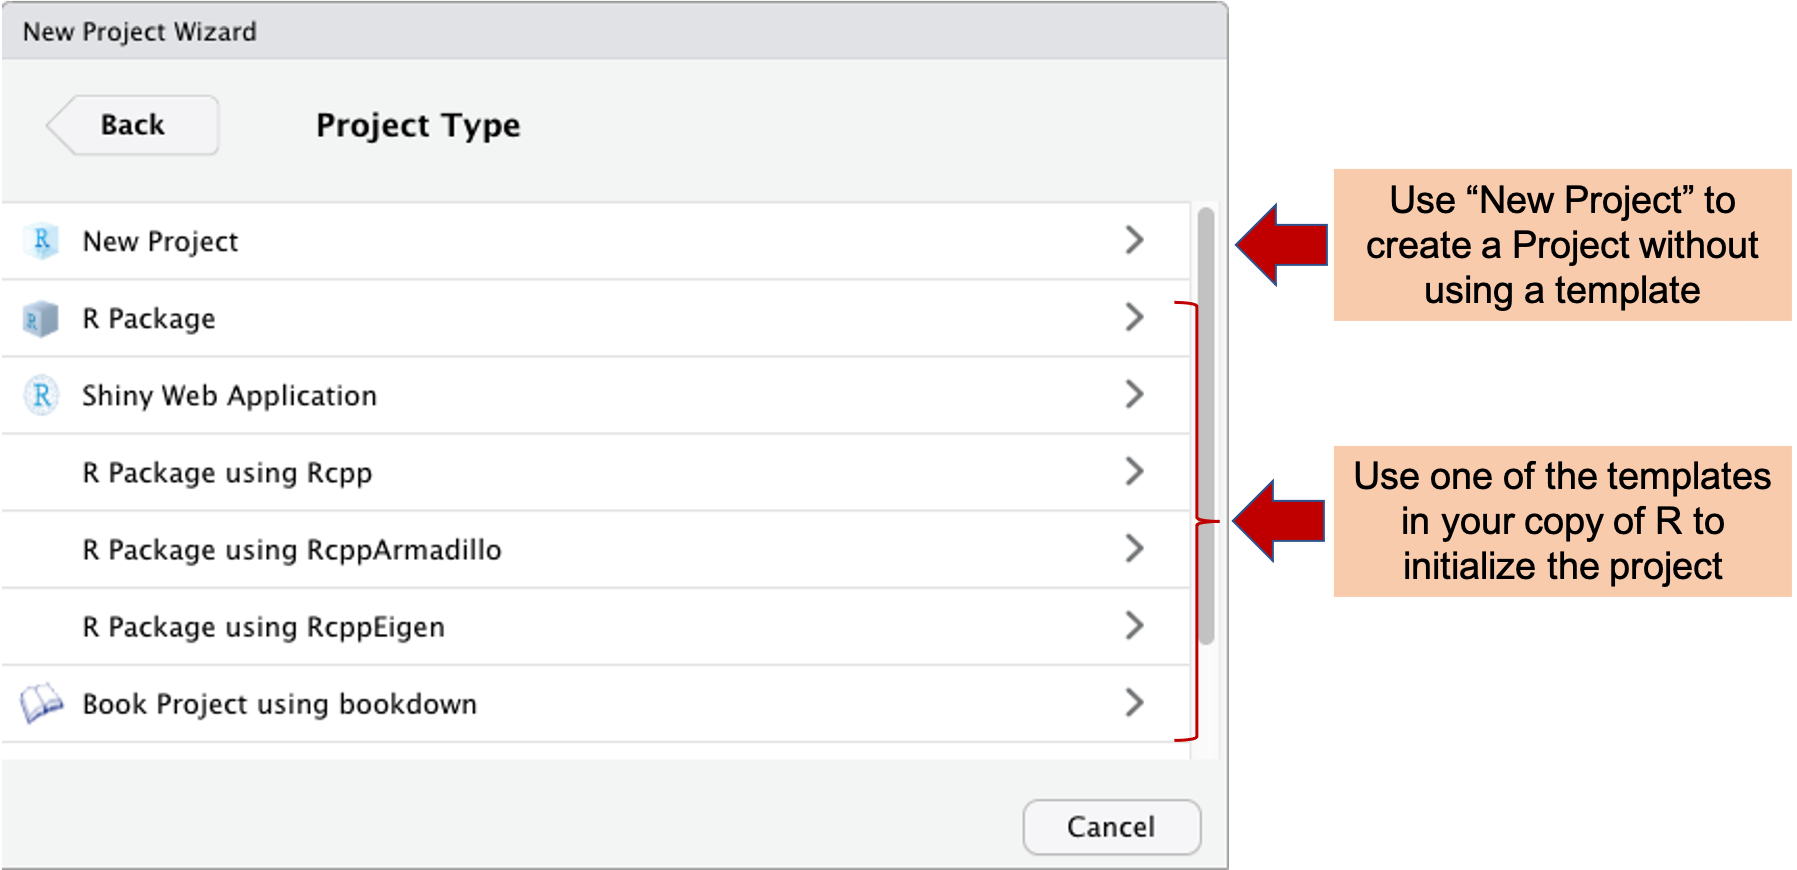
\includegraphics[width=\textwidth]{figures/create_new_project} \caption[Creating a new project in RStudio]{Creating a new project in RStudio. When you chose 'File' then 'New Project' from the RStudio menu, it opens the New Project Wizard shown here. You have the option to create a new project that is not based on a project template by selecting 'New Project'. You also have the chance to create a project using a template by selecting one of the templates. The listed templates will depend on which packages you have downloaded for your copy of R. For example, here the `bookdown` package has been installed for the local copy of R, and so a template is available for 'Book Project using bookdown'.}\label{fig:createnewproject}
\end{figure*}

This pop-up contains the New Project Wizard in RStudio. Here, you can either
create a new Project without using a template (click on ``New Project'') or you
can create a Project starting from a template. The templates available in your
copy of R will be listed below the ``New Project'' listing. Depending on which
packages you've installed for your copy of R, you will have different choices of
project templates available, as project templates tend to be created and shared
within R packages \citep{rstudioprojecttemplate}. In the example shown in
Figure \ref{fig:createnewproject}, for example, one of the template options is
for a ``Book Project using bookdown'', available because the \texttt{bookdown} R package
has been installed locally.

Your research group can create your own Project templates. You will need to
create them within an R package, but this package does not need to be posted to
a public site like CRAN. Instead, it can be shared exclusively among the
research group as a zipped file that can be installed directly from source onto
each person's computer. Alternatively, you can post the package code as a GitHub
repository, and there are straightforward tools for installing R package code
from GitHub onto each team member's computer. RStudio has provided a
detailed guide to creating your own project template at
\url{https://rstudio.github.io/rstudio-extensions/rstudio_project_templates.html}.
This topic has also been discussed through a short talk at the
yearly RStudio::conf: \url{https://rstudio.com/resources/rstudioconf-2020/rproject-templates-to-automate-and-standardize-your-workflow/}.

\begin{quote}
``RStudio v1.1 introduces support for custom, user-defined project templates.
Project templates can be used to create new projects with a pre-specified
structure.'' \citep{rstudioprojecttemplate}
\end{quote}

\begin{quote}
``R packages are the primary vehicle through which RStudio project templates
are distributed. Package authors can provide a small bit of metadata describing
the template functions available in their package---RStudio will discover these
project templates on start up, and make them available in the New Project\ldots{}
dialog.'' \citep{rstudioprojecttemplate}
\end{quote}

\begin{quote}
``R experts keep all the files associated with a project together---input data,
R scripts, analytical results, figures. This is such a wise and common practice
that RStudio has built-in support for this via \textbf{projects}.'' \citep{wickham2016r}
\end{quote}

\hypertarget{discussion-questions-2}{%
\subsection{Discussion questions}\label{discussion-questions-2}}

\hypertarget{module8}{%
\section{Example: Creating a `Project' template}\label{module8}}

We will walk through a real example, based on the experiences of one of our
Co-Is, of establishing the format for a research group's `Project' template,
creating that template using RStudio, and initializing a new research project
directory using the created template. This example will be from a
laboratory-based research group that studies the efficacy of tuberculosis drugs
in a murine model.

\textbf{Objectives.} After this module, the trainee will be able to:

\begin{itemize}
\tightlist
\item
  Create a `Project' template in RStudio to initialize consistently-formatted
  `Project' directories
\item
  Initialize a new `Project' directory using this template
\end{itemize}

\hypertarget{subsection-1-2}{%
\subsection{Subsection 1}\label{subsection-1-2}}

\hypertarget{subsection-2-1}{%
\subsection{Subsection 2}\label{subsection-2-1}}

\hypertarget{applied-exercise-2}{%
\subsection{Applied exercise}\label{applied-exercise-2}}

\hypertarget{module9}{%
\section{Harnessing version control for transparent data recording}\label{module9}}

As a research project progresses, a typical practice in many experimental
research groups is to save new versions of files (e.g., `draft1.doc',
`draft2.doc'), so that changes can be reverted. However, this practice leads to
an explosion of files, and it becomes hard to track which files represent the
`current' state of a project. Version control allows researchers to edit and
change research project files more cleanly, while maintaining the power to
`backtrack' to previous versions, messages included to explain changes. We will
explain what version control is and how it can be used in research projects to
improve the transparency and reproducibility of research, particularly for data
recording.

\textbf{Objectives.} After this module, the trainee will be able to:

\begin{itemize}
\tightlist
\item
  Describe version control\\
\item
  Explain how version control can be used to improve reproducibility
  for data recording
\end{itemize}

\hypertarget{what-is-version-control}{%
\subsection{What is version control?}\label{what-is-version-control}}

Version control developed as a way to coordinate collaborative work on software
programming projects. The term ``version'' here refers to the current state of a
document or set of documents, for example the source code for a computer
program. The idea of ``control'' is to allow for safe changes and updates to this
version while more than one person is working on it. The general term ``version
control'' can refer to any method of syncing contributions from several people to
a file or set of files, and very early on it was done by people rather than
through a computer program. While version control of computer files can be done
by people, and originally was \citep{irving2011astonishments}, it's much more
efficient to use a computer program to handle this tracking of the history of a
set of files as they evolve.

\begin{quote}
``Tracking all that detail is just the sort of thing computers
are good at and humans are not.'' \citep{raymond2003art}
\end{quote}

While the very earliest version control systems tracked single files, these
systems quickly moved to tracking sets of files, called \emph{repositories}. You can
think of a repository as a computer file directory with some extra overhead
added to record how the files in the directory have changed over time. In a
repository of files that is under version control, you take regular ``snapshots''
of how the files look during your work on them. Each snapshot is called a
\emph{commit}, and it provides a record of which lines in each file changed from one
snapshot to another, as well as exactly how they changed. The idea behind these
commits---recording the differences, line-by-line, between an older and newer
version of each file derives from a longstanding Unix command line tool called
\texttt{diff}. This tool, developed early in the history of Unix at AT\&T
\citep{raymond2003art}, is and extremely solid and well-tested tool that did the
simple but important job of generating a list of all the differences between two
plain text files.

When you are working with a directory under version control, you can also
explain your changes as you make them---in other words, it allows for
\emph{annotation} of the developing and editing process \citep{raymondunderstanding}. Each
commit requires you to enter a \emph{commit message} describing why the change was
made. The commit messages can serve as a powerful tool for explaining changes to
other team members or for reminding yourself in the future about why certain
changes were made. As a result, a repository under version control includes a
complete history of how files in a project directory have changed over the
timecourse of the project and why. Further, each of the commits is given its own
ID tag (a unique SHA-1 hash), and version control systems have a number of
commands that let you ``roll back'' to earlier versions, by going back to the
version as it was when a certain commit was made, provided \emph{reversability}
within the project files \citep{raymondunderstanding}.

It turns out that this functionality---of being able to ``roll back'' to earlier
versions---has a wonderful side benefit when it comes to working on a large
project. It means that you \emph{don't} need to save earlier versions of each file.
You can maintain one and only one version of each project file in the project's
directory, with the confidence that you never ``lose'' old versions of the file
\citep{perkel2018git, blischak2016quick}. This allows you to maintain a clean and
simple version of the project files, with only one copy of each, ensuring it's
always clear which version of a file is the ``current'' one (since there's only
one version). This also provides the reassurance that you can try new directions
in a project, and always roll back to the old version if that direction doesn't
work well.

\begin{quote}
``Early in his graduate career, John Blischak found himself creating figures
for his advisor's grant application. Blischak was using the programming language
R to generate the figures, and as he iterated and optimized his code, he ran
into a familiar problem: Determined not to lose his work, he gave each new
version a different filename---analysis\_1, analysis\_2, and so on, for
instance---but failed to document how they had evolved. `I had no idea what had
changed between them,' says Blischak\ldots{} Using Git, Blischak says, he no longer
needed to maintain multiple copies of his files. `I just keep overwriting it and
changing it and saving the snapshots. And if the professor comes back and says,
'oh, you sent me an email back in March with this figure', I can say, `okay,
well, I'll just bo back to the March version of my code and I can recreate
it'.'' \citep{perkel2018git}
\end{quote}

Finally, most current version control systems operate under a \emph{distributed}
framework. In earlier types of version control programs, there was one central
(``main'') repository for the file or set of files the team was working on
\citep{raymondunderstanding, target2018version}. Very early on, this was kept on one
computer \citep{irving2011astonishments}. A team member who wanted to make a change
would ``check out'' the file he or she wanted to work on, make changes, and then
check it back in as the newest main version \citep{raymond2003art}. While one team
member had this file checked out, other members would often be ``locked'' out of
making any changes to that file---they could look at it, but couldn't make any
edits \citep{raymondunderstanding, target2018version}. This meant that there was no
chance of two people trying to change the same part of a file at the same time.
In spirit, this early system is pretty similar to the idea of sending a file
around the team by email, with the understanding that only one person works on
it at a time. While the ``main'' version is in different people's hands at
different times, to do work, you all agree that only one person will work on it
at a time. A slightly more modern analogy is the idea of having a single version
of a file in Dropbox or Google Docs, and avoiding working on the file when you
see that another team member is working on it.

This system is pretty clunky, though. In particular, it usually increases the
amount of time that it takes the team to finish the project, because only one
person can work on a file at a time. Later types of version control programs
moved toward a different style, allowing for \emph{distributed} rather than
\emph{centralized} collaborative work on a file or a set of files
\citep{raymondunderstanding, irving2011astonishments}. Under the distributed model,
all team members can have their own version of all the files, work on them and
make records of changes they make to the files, and then occassionally sync with
everyone else to share your changes with them and bring their changes into your
copy of the files. This distributed model also means there is a copy of the full
repository on every team members computer, which has the side benefit of
provided natural backup of the project files. Remote repositories---which may be
on a server in a different location---can be added with another copy of the
project, which can similarly be synced regularly to update with any changes made
to project files.

While there are a number of software systems for version control, by far the
most common currently used for scienctific projects is \emph{git}. This program was
created by Linus Torvalds, who also created the Linux operating system, in 2005
as a way to facilitate the team working on Linux development. This program for
version control thrives in large collaborative projects, for example open-source
software development projects that include numerous contributors, both regular
and occasional \citep{brown2018git}.

In recent years, some complementary tools have been developed that make the
process of collaborating together using version control software easier. Other
tools can helps in collaborating on file-based projects, including \emph{bug
trackers} or \emph{issue trackers}, which allow the team to keep a running ``to-do''
list of what needs to be done to complete the project, all of which are
discussed in the next chapter as tools that can be used to improve collaboration
on scientific projects spread across teams. GitHub, a very popular version
control platform with these additional tools, was created in 2008 as a web-based
platform to facilitate collaborating on projects running under git version
control. It can provide an easier entry to using git for version control than
trying to learn to use git from the command line \citep{perez2016ten}. It also plays
well with RStudio, making it easy to integrate a collaborative workflow through
GitHub from the same RStudio window on your computer where you are otherwise
doing your analysis \citep{perez2016ten}.

\begin{quote}
``If your software engineering career, like mine, is no older than GitHub, then
git may be the only version control software you have ever used. While people
sometimes grouse about its steep learning curve or unintuitive interface, git has
become everyone's go-to for version control.'' \citep{target2018version}
\end{quote}

\hypertarget{recording-data-in-the-laboratoryfrom-paper-to-computers}{%
\subsection{Recording data in the laboratory---from paper to computers}\label{recording-data-in-the-laboratoryfrom-paper-to-computers}}

Traditionally, experimental data collected in a laboratory was recorded in a
paper laboratory notebook. These laboratory notebooks played a role not only as
the initial recording of data, but also can serve as, for example, a legal
record of the data recorded in the lab \citep{mascarelli2014research}. They were also
a resource for collaborating across a team and for passing on a research project
from one lab member to another \citep{butler2005electronic}.

However, paper laboratory notebooks have a number of limitations. First, they
can be very inefficient. In a time when almost all data analyses---even simple
calculations---are done on a computer, recording research data on paper rather
than directly entering it into a computer is inefficient. Also, any stage of
copying data from one format to another, especially when done by a human rather
than a machine, introduces the chance to copying errors. Handwritten laboratory
notebooks can be hard to read \citep{butler2005electronic, perkel2011coding}, and
may lack adequate flexibility and expandability to handle the complex
experiments often conducted. Further, electronic alternatives can also be easier
to search, allowing for deeper and more comprehensive investigations of the data
collected across multiple experiments \citep{giles2012digital, butler2005electronic, perkel2011coding}.

\begin{quote}
``Handwritten lab notebooks are usually chaotic and always unsearchable.''
\citep{perkel2011coding}
\end{quote}

Given a widespread recognition of the limitations of paper laboratory notebooks,
in the past couple of decades, there have been a number of efforts, both formal
and informal, to move from paper laboratory notebooks to electronic
alternatives. In some fields that rely heavily on computational analysis, there
are very few research labs (if any) that use paper laboratory notebooks
\citep{butler2005electronic}. In other fields, where researchers have traditionally
used paper lab notebooks, companies have been working for a while to develop
electronic laboratory notebooks specifically tailored to scientific research
needs \citep{giles2012digital}. These were adopted more early in pharmaceutical
industrial labs, where companies had the budgets to get customized versions and
the authority to require their use, but have taken longer to be adapted in
academic laboratories \citep{giles2012digital, butler2005electronic}. A widely
adopted platform for electronic laboratory notebooks has yet to be taken up
by the scientific community, despite clear advantages of recording data directly
into a computer rather than first using a paper notebook.

\begin{quote}
``Since at least the 1990s, articles on technology have predicted the imminent,
widespread adoption of electronic laboratory notebooks (ELNs) by researchers. It has
yet to happen---but more and more scientists are taking the plunge.'' \citep{kwok2018lab}
\end{quote}

Instead of using customized electronic laboratory notebook software, some
academics are moving their data recording online, but are using more generalized
electronic alternatives, like Dropbox, Google applications, OneNote, and
Evernote \citep{perkel2011coding, kwok2018lab, giles2012digital, powell2012lab}.
Some scientists have started using version control tools, especially the
combination of git and GitHub, as a way to improve laboratory data recording,
and in particular to improve transparency and reproducibility standards.
These pieces of software share the same pattern as Google tools or
Dropbox---they are generalized tools that have been honed and optimized for ease
of use through their role outside of scientific research, but can be harnessed
as a powerful tool in a scientific laboratory, as well. They are also free---at
least, for GitHub, at the entry and academic levels---and, even better, one
(git) is open source.

\begin{quote}
``The purpose of a lab notebook is to provide a lasting record of events in a
laboratory. In the same way that a chemistry experiment would be nearly
impossible without a lab notebook, scientific computing would be a nightmare of
inefficiency and uncertainty without version-control systems.''
\citep{tippmannmy2014digital}
\end{quote}

While some generalized tools like Google tools and Dropbox might be simpler to
initially learn, version control tools offer some key advantages for recording
scientific data and are worth the effort to adopt. A key advantage is their
ability to track the full history of files as they evolve, including not only
the history of changes to each file, but also a record of why each change was
made. Git excels in tracking changes made to plain text
files. For these files, whether they record code, data, or text, git can show
line-by-line differences between two versions of the file. This makes it very
easy to go through the history of ``commits'' to a plain text file in a
git-tracked repository and see what change was made at each time point, and then
read through the commit messages associated with those commits to see why a
change was made. For example, if a value was entered in the wrong row of a csv,
and the researcher then made a commit to correct that data entry mistake, the
researcher could explain the problem and its resolution in the commit message
for that change.

Platforms for using git often include nice tools for visualizing differences
between two files, providing a more visual way to look at the ``diffs'' between
files across time points in the project. For example, GitHub automatically shows
these using colors to highlight addititions and substractions of plain text for
one file compared to another version of it when you look through a repository's
commit history. Similarly, RStudio provides a new ``Commit'' window that can be
used to compare differences between the original and revised version of plain
text files at a particular stage in the commit history.

The use of version control tools and platforms, like git and GitHub, not only
helps in transparent and trackable recording of data, but it also brings some
additional advantages in the research project. First, this combination of tools
aids in collaboration across a research group, as we discuss in depth in the next
chapter.

Second, if a project uses these tools, it is very easy to share data recorded
for the project publicly. In a project that uses git and GitHub version control
tools, it is easy to share the project data online once an associated manuscript
is published, an increasingly common request or requirement from journals and
funding agencies \citep{blischak2016quick}. Sharing data allows a more complete
assessment of the research by reviewers and readers and makes it easier for
other researchers to build off the published results in their own work,
extending and adapting the code to explore their own datasets or ask their own
research questions \citep{perez2016ten}. On GitHub, you can set the access to a
project to be either public or private, and can be converted easily from one
form to the other over the course of the project \citep{metz2015github}. A private
project can be viewed only by fellow team members, while a public project can be
viewed by anyone. Further, because git tracks the full history of changes to
these documents, it includes functionality that let's you tag the code and data
at a specific point (for example, the date when a paper was submitted) so that
viewers can look at that specific ``version'' of the repository files, even while
the project team continues to move forward in improving files in the directory.
At the more advanced end of functionality, there are even ways to assign a DOI
to a specific version of a GitHub repository \citep{perez2016ten}.

Third, the combination of git and GitHub can help as a way to backup study data
\citep{blischak2016quick, perez2016ten, perkel2018git}. Together, git and GitHub
provide a structure where the project directory (repository) is copied on
multiple computers, both the users' laptop or desktop computers and on a remote
server hosted by GitHub or a similar organization. This set-up makes it easy to
bring all the project files onto a new computer---all you have to do is clone
the project repository. It also ensures that there are copies of the full
project directory, including all its files, in multiple places
\citep{blischak2016quick}. Further, not only is the data backed up across multiple
computers, but so is the full history of all changes made to that data and the
recorded messages explaining those changes, through the repositories commit
messages \citep{perez2016ten}.

There are, of course, some limitations to using version control tools when
recording experimental data. First, while ideally laboratory data is recorded in
a plain text format (see the module in section 2.2 for a deeper discussion of
why), some data may be recorded in a binary file format. Some version control
tools, including git, can be used to track changes in binary files. However, git
does not take to these types of files naturally. In particular, git typically
will not be able to show users a useful comparison of the differences between
two versions of a binary file. More problems can arise if the binary file is
very large \citep{perez2016ten, blischak2016quick}, as some experimental research
data files are (e.g., if they are high-throughput output of laboratory equipment
like a mass spectrometer). However, there are emerging tools and strategies for
improving the ability to include and track large binary files when using git and
GitHub \citep{blischak2016quick}

\begin{quote}
``You can version control any file that you put in a Git repository, whether it is
text-based, an image, or a giant data file. However, just because you \emph{can} version
control something, does not mean that you \emph{should}.'' \citep{blischak2016quick}
\end{quote}

Finally, as with other tools and techniques described in this book, there is an
investment required to learn how to use git and GitHub \citep{perez2016ten}, as well
as a bit of extra overhead when using version control tools in a project
\citep{raymond2003art}. However, both can bring dramatic gains to efficiency,
transparency, and organization of research projects, even if you only use a
small subset of its basic functionality \citep{perez2016ten}. In Chapter 11 we
provide guidance on getting started with using git and Github to track a
scientific research project.

\begin{quote}
``Although Git has a complex set of commands and can be used for rather complex
operations, learning to apply the basics requires only a handful of new concepts
and commands and will provide a solid ground to efficiently track code and related
content for research projects.'' \citep{perez2016ten}
\end{quote}

\hypertarget{discussion-questions-3}{%
\subsection{Discussion questions}\label{discussion-questions-3}}

\begin{center}\rule{0.5\linewidth}{0.5pt}\end{center}

\begin{quote}
``Using an RCS {[}revision control system{]} has changed how I work. \ldots{} a day's
work is no longer a featureless slog toward the summit, but a sequence of small
steps. What one feature could I add? What one problem could I fix? Once a step is
made and you are sure your code base is in a safe and clean state, commit a revision,
and if your next step turns out disastrously, you can fall back to the revision you
just committed instead of starting from the beginning.'' \citep{klemens201421st}
\end{quote}

\begin{quote}
With version control, ``Our filesystem now has a time dimension. We can query the
RCS's repository of file information to see what a file looked like last week and
how it changed from then to now. Even without the other powers, I have found that
this alone makes me a more confident writer.'' \citep{klemens201421st}
\end{quote}

\begin{quote}
``The most rudimentary means of revision control is via \texttt{diff} and \texttt{patch}, which
are POSIX-standard and therefore most certainly on your system.'' \citep{klemens201421st}
\end{quote}

\begin{quote}
``Git is a C program like any other, and is based on a small set of objects.
The key object is the commit object, which is akin to a unified diff file.
Given a previous commit object and some changes from that baseline, a new commit
object encapsulates the information. It gets some support from the \emph{index}, which
is a list of the changes registered since the last commit object, the primary
use of which will be in generating the next commit object. The commit objects
link together to form a tree much like any other tree. Each commit object will
have (at least) one parent commit object. Stepping up and down the tree is akin to
using \texttt{patch} and \texttt{patch\ -R} to step among versions.'' \citep{klemens201421st}
\end{quote}

\begin{quote}
``Having a backup system organized enough that you can delete code with confidence
and recover as needed will already make you a better writer.'' \citep{klemens201421st}
\end{quote}

\hypertarget{module10}{%
\section{Enhance the reproducibility of collaborative research with version control platforms}\label{module10}}

Once a researcher has learned to use \emph{git} on their own computer for
local version control, they can begin using version control platforms (e.g.,
\emph{GitLab}, \emph{GitHub}) to collaborate with others under version
control. We will describe how a research team can benefit from using a version
control platform to work collaboratively.

\textbf{Objectives.} After this module, the trainee will be able to:

\begin{itemize}
\tightlist
\item
  List benefits of using a version control platform to collaborate
  on research projects, particularly for reproducibility
\item
  Describe the difference between version control (e.g., \emph{git}) and
  a version control platform (e.g., \emph{GitLab})
\end{itemize}

\hypertarget{what-are-version-control-platforms}{%
\subsection{What are version control platforms?}\label{what-are-version-control-platforms}}

The last module introduced the idea of version control, including the
popular software tool often used for version control, \emph{git}. In this
module, we'll go a step further, telling you about how you can expand
the idea of version control to leverage it when collaborating across
your research team, using \textbf{version control platforms}.

When research groups---or any other professional teams---collaborate on
publications and research, the process can be a bit haphazard. Teams often use
emails and email attachments to share updates on the project, and email
attachments to pass around the latest version of a document for others to review
and edit. For example, one group of researchers investigated a large collection
of emails from Enron \citep{hermans2015enron}. They found that passing Excel files
through email attachements was a common practice, and that messages within
emails suggested that spreadsheets were stored locally, rather than in a
location that was accessible to all team members \citep{hermans2015enron}, which
meant that team members might often be working on different versions of the same
spreadsheet file. They note that ``the practice of emailing spreadsheets is known
to result in serious problems in terms of accountability and errors, as people
do not have access to the latest version of a spreadsheet, but need to be
updated of changes via email.'' \citep{hermans2015enron} The same process for
collaboration is often used in scientific research, as well: one study found,
``Team members regularly pass data files back and forth by hand, by email, and by
using shared lab or project servers, websites, and databases.''
\citep{edwards2011science}

\begin{quote}
``The most primitive (but still very common) method {[}of version control{]} is all
hand-hacking. You snapshot the project periodically by manually copying
everything in it to a backup. You include history comments in source files. You
make verbal or email arrangements with other developers to keep their hands off
certain files while you hack them. \ldots{} The hidden costs of this hand-hacking
method are high, especially when (as frequently happens) it breaks down. The
procedures take time and concentration; they're prone to error, and tend to get
slipped under pressure or when the project is in trouble---that is exactly when
they are needed.'' \citep{raymond2003art}
\end{quote}

These practices make it very difficult to keep track of all project files,
and in particular, to track which version of each file is the most current.
Further, this process constrains patterns of collaboration---it requires
each team member to take turns in editing each file, or for one team member
to attempt to merge in changes that were made by separate team members at
the same time when all versions are collected. Further, this process makes
it difficult to keep track of why changes were made, and often requires
one team member to approve the changes of other team members. While the
``Track changes'' and comment features can help the team communicate with
each other, but these features often lead to a very messy document at
stages in the editing, where it is hard to pick out the current versus
suggested wording, and once a change is accepted or a comment deleted,
these conversations are typically lost forever. Finally, word processing
tools are poorly suited to track changes or add suggestions directly to
data or code, as both data and code are usually saved in formats that
aren't native to word processing programs, and copying them into a format
like Word can introduce problematic hidden formatting that can cause the
data or code to malfunction.

A version control platform allows you to share project files across a group of
collaborators while keeping track of what changes are made, who made each
change, and why each change was made. It therefore combines the strengths of a
``Track changes'' feature with those of a file sharing platform like Dropbox. To
some extent, Google Docs or Google Drive also combine these features, and some
spreadsheet programs are moving toward some rudimentary functionality for
version control \citep{birch2018future}. However, there are added advantages of
version control platforms. Since open-source version control platforms like
GitHub can be set up on a server that you own, they can be used to collaborate
on projects with sensitive data, and also can store data directly on the server
you would like to use to store large project datasets or to run
computationally-intensive pre-processing or analysis. Finally, most version
control platforms include tools that help you manage and track the project.
These include ``Issue Trackers'', tools for exploring the history of each file
and each change, and features to assign project tasks to specific team members.
The next section will describe the features of version control platforms that
make them helpful as a tool for collaborating on scientific research. These
systems are being leveraged by some scientists, both to manage research projects
and also to collaborate on writing scientific manuscripts and grant proposals
\citep{perez2016ten}.

\begin{quote}
``Using GitHub or any similar versioning / tracking system is not a replacement
for good project management; it is an extension, an improvement for good
project and file management.'' \citep{perez2016ten}
\end{quote}

Version control platforms are always used in conjunction with version control
software, like the \emph{git} software described in the last module. Version control
itself has been described as ``a suite of programs that automates away most of
the drudgery involved in keeping an annotated history of your project and
avoiding modification conflicts,'' \citep{raymond2003art}. The version control
platform leverages the history of commits that were made to the project, as well
as the version control software's capabilities for merging changes made by
different people at different times. On top of these facilities, a version
control platform also adds attractive visual interfaces for working with the
project, free or low-cost online hosting of project files, and team management
tools for each project. You can think of \emph{git} as the engine, in other words,
and the version control platform as the driver's seat, with dashboard, steering
wheel, and gears to leverage the power of the underlying \emph{git} software.

A number of version control platforms are available. Two that are currently very
popular for scientific research are GitHub (\url{https://github.com/}) and GitLab
(\url{https://about.gitlab.com/}). Both provide free options for scientific
researchers, including the capabilities for using both public and private
repositories in collaboration with other researchers.

\begin{quote}
Resources like GitHub are ``essential for collaborative software projects
because they enable the organization and sharing of programming tasks between
different remote contributors.'' \citep{perez2016ten}
\end{quote}

\hypertarget{why-use-version-control-platforms}{%
\subsection{Why use version control platforms?}\label{why-use-version-control-platforms}}

Version control platforms offer a number of advantages when collaborating
on a research project that can help to improve your efficiency, rigor, and
reproducibility. Further, there are several high-quality free versions
of version control platforms that are available for researchers, and as
their use becomes more popular, resources for learning the details of how
to use these platforms effectively. Open-source versions, like GitLab,
even allow you to set up a version control platform on a server you own,
rather than needing to post data or code on an outside platform, and so
you can use these tools even in cases of sensitive data.

Some of the key advantages of using a version control platform like GitHub
to collaborate on research projects include:

\begin{itemize}
\tightlist
\item
  Ability to track and merge changes that different collaborators made to the
  document
\item
  Ability to create alternative versions of project files (\emph{branches}), and merge them into the main project as desired
\item
  Tools for project management, including Issue Trackers
\item
  Default backup of project files
\item
  Ability to share project information online, including through hosting websites related to the project or supplemental files related to a manuscript
\end{itemize}

Many of these strengths draw directly on the functions provided by the
underlying version control software (e.g., \emph{git}). However, the version control
platform will typically allow team members to explore and work with these
functions in an easier way than if they try to use the barebones version control
software. In earlier years, the use of version control often required users to
be familiar with the command line, and to send arcane commands to track the
project files through that interface. With the rising popularity of version
control platforms, version control for project management can be taught
relatively quickly to students with a few months---or even weeks---of coding
experience. In fact, version control is beginning to be used as a method of
turning in and grading homework in beginning programming classes, with students
learning these techniques in the first few weeks of class. This would be
practically unimaginable without the user-friendly interface of a version
control platform as a wrapper for the power of the version control software
itself.

\begin{quote}
``One reason for GitHub's success is that it offers more than a simple source
code hosting service. It provides developers and researchers with a dynamic and
collaborative environment, often referred to as a social coding platform, that
supports peer review, commenting, and discussion. A diverse range of efforts,
ranging from individual to large bioinformatics projects, laboratory
repositories, as well as global collaborations, have found GitHub to be a
productive place to share code and ideas and collaborate.'' \citep{perez2016ten}
\end{quote}

The first strength of using version control---and a version control
platform---to collaborate on scientific projects is its ability to track every
change made to files in the project, why the change was made, and who made it.
Version control creates a full history of the evolution of each file in the
project. When a change is committed, the history records the exact change made,
including the previous version of the file. No change is ever fully lost,
therefore, unless a great deal of extra work is taken to erase something from
the project's commit history. Version control also requires a user to provide a
\emph{commit message} describing each change that is made. If this feature is used
thoughtfully, then the commit history of the project provides a well-documented
description of the project's full evolution. If you're working on a manuscript,
for example, when it's time to edit, you can cut whole paragraphs, and if you
ever need to get them back, they'll be right there in the commit history for
your project, with their own commit message about why they were cut (hopefully a
nice clear one that will make it easy to find that commit if you ever need those
paragraphs again).

\begin{quote}
``{[}Version control systems{]} are a huge boon to productivity and code quality in
many ways, even for small single-developer projects. They automate away many
procedures that are just tedious work. They help a lot in recovering from
mistakes. Perhaps most importantly, they free programmers to experiment by
guarnateeing that reversion to a known-good state will always be easy.''
\citep{raymond2003art}
\end{quote}

These capacities to track changes and histories of project files becomes even
more important when working in collaboration on a project. As the proverb about
too many cooks in the kitchen captures, any time you have multiple people
working on a project, it introduces the chance for conflicts. While higher-level
conflicts, like about what you want the final product to look like or who should
do which jobs, can't be easily managed by a computer program, now the
complications of integrating everyone's contributions---and letting people work
in their own space and then bring together their individual work into one final
joint project---can be. While these programs for version control were originally
created to help with programmers developing code, they can be used now to
coordinate group work on numerous types of file-based projects, including
scientific manuscripts, books, and websites \citep{raymondunderstanding}. And
although they can work with projects that include binary code, they thrive in
projects with a heavier concentration of text-based files, and so they fit in
nicely in a scientific research / data analysis workflow that is based on data
stored in plain text formats and data analysis scripts written in plain text
files, tools we discuss in other parts of this book.

\begin{quote}
``In a medium-sized project, it often happens that a (relatively small) number
of people work simultaneously on a single set of files, the `program' or the
`project'. Often these people have additional tasks, causing their working
speeds to differ greatly. One person may be working a steady ten hours a day on
the project, a second may have barely time to dabble in the project enough to
keep current, while a third participant may be sent off on an urgent temporary
assignment just before finishing a modification. It would be nice if each
participant could be abstracted from the vicissitudes of the lives of the
others.'' \citep{grune1986concurrent}
\end{quote}

Modern version control systems like \emph{git} take a distributed approach to
collaboration on project files. Under the distributed model, all team members
can have their own version of all the files, work on them and make records of
changes they make to the files, and then occassionally sync with everyone else
to share your changes with them and bring their changes into your copy of the
files. This functionality is called \emph{concurrency}, since it allows team members
to concurrently work on the same set of files \citep{raymondunderstanding}. This idea
allowed for the development of other useful features and styles of working,
including \emph{branching} to try out new ideas that you're not sure you'll
ultimately want to go with and \emph{forking}, a key tool used in open-source
software development, which among other things facilitates someone who isn't
part of the original team getting a copy of the files they can work with and
suggesting some changes that might be helpful. So, this is the basic idea of
modern version control---for a project that involves a set of computer files,
everyone on the team (even if that's just one person) has their own copy of a
directory with those files on their own computer, makes changes at the time and
in the spots in the files that they want, and then regularly re-syncs their
local directory with everyone else's to share changes and updates.

There is one key feature of modern version control that's critical to making
this work---merging files that started the same but were edited in different
ways and now need to be put back together, bringing any changes made from the
original version. This step is called \emph{merging} the files. While this is
typically described using the plural, ``files'', at a higher-level, you can thing
of this as just merging the \emph{changes} that two people have made as they edited a
single file, a file where they both started out with identical copies.

Think of the file broken up into each of its separate lines. There will be some
lines that neither person changed. Those are easy to handle in the
``merge''---they stay the same as in the original copy of the file. Next, there
will be some lines that one person changed, but that the other person didn't. It
turns out that these are pretty easy to handle, too. If only one person changed
the line, then you use their version---it's the most up-to-date, since if both
people started out with the same version, it means that the other person didn't
make any changes to that part of the file. Finally, there may be a few lines
that both people changed. These are called \emph{merge conflicts}. They're places in
the file where there's not a clear, easy-to-automate way that the computer can
know which version to put into the integrated, latest version of the file.
Different version control programs handle these merge conflicts in different
ways. For the most common version control program used today, \emph{git}, these spots
in the file are flagged with a special set of symbols when you try to integrate
the two updated versions of the file. Along with the special symbols to denote a
conflict, there will also be \emph{both} versions of the conflicting lines of the
file. Whoever is integrating the files must go in and pick the version of those
lines to use in the integrated version of the file, or write in some compromise
version of those lines that brings in elements from both people's changes, and
then delete all the symbols denoting that was a conflict and save this latest
version of the file.

\begin{quote}
``You will likely share your code with multiple lab mates or collaborators,
and they may have suggestions on how to improve it. If you email the code
to multiple people, you will have to manually incorporate all the changes
each of them sends.'' \citep{blischak2016quick}
\end{quote}

There are a number of other features of version control that make it useful for
collaborating on file-based projects with teams. First, these systems allow you
to explain your changes as you make them---in other words, it allows for
\emph{annotation} of the developing and editing process \citep{raymondunderstanding}. This
provides the team with a full history of why the files evolved in the way they
did across the team. It also provides a way to communicate across the team
members.

For example, if one person is the key person working on a certain file,
but has run into a problem with one spot and asks another team member to take a
go, then the second team member isn't limited to just looking at the file and
then emailing some suggestions. Instead, the second person can make sure he or
she has the latest version of that file, make the changes they think will help,
\emph{commit} those changes with a message (a \emph{commit message}) about why they think
this change will fix the problem, and then push that latest version of the file
back to the first person. If there are several places where it would help to
change the file, then these can be fixed through several separate commits, each
with their own message. The first person, who originally asked for help, can
read through the updates in the file (most platforms for using version control
will now highlight where all these changes are in the file) and read the second
person's message or messages about why each change might help. Even better, days
or months later, when team members are trying to figure out why a certain change
was made in that part of the file, can go back and read these messages to get an
explanation.

\begin{quote}
``You know your code has changed; do you know why? It's easy to forget the
reasons for changes, and step on them later. If you have collaborators on a
project, how do you know what they have changed while you weren't looking, and
who was responsible for each change?'' \citep{raymond2003art}
\end{quote}

In recent years, some complementary tools have been developed that make the
process of collaborating together using version control software easier. Other
tools can helps in collaborating on file-based projects, including \emph{bug
trackers} or \emph{issue trackers}, which allow the team to keep a running ``to-do''
list of what needs to be done to complete the project, all of which are
discussed in the next chapter \citep{perez2016ten}.

Finally, version control platforms like GitHub can be used for a number
of supplementary tasks for your research project. These include publishing
webpages or other web resources linked to the project and otherwise improving
public engagement with the project, including by allowing other researchers
to copy and adapt your project through a process called \emph{forking}. Version
control platforms also provide a supplemental backup to project files.

First, GitHub can be used to collaborate on, host, and publish websites and
other online content \citep{perez2016ten}. Version control systems have been used by
some for a long time to help in writing longform materials like books (e.g.,
\citep{raymond2003art}); new tools are making the process even easier. Thethe GitHub
Pages functionality, for example, is now being used to host a number of books
created in R using the \texttt{bookdown} package, including the online version of this
book. The \texttt{blogdown} package similarly can be used to create websites, either
for individual researchers, for research labs, or for specific projects or
collaborations. Further, if a project includes the creation of scientific
software, it can be used to share that software---as well as associated
documentation---in a format that is easy for others to work with. The platform
can also be used to share supplemental material for a manuscript, including the
code used for preprocessing and analyzing data. The most popular version control
platforms, GitHub and GitLab, both allow users to toggle projects between
``public'' and ``private'' modes, which can be used to work privately on a
project prior to peer review and publication, and then switch to a public mode
after publication. This functionality will allow those who access the code to
see not only the final product, but also the history of the development of the
code and data for the project, providing more transparency in the development
process, but without jeopardizing the novelty of the research results prior to
publication.

\begin{quote}
``The traditional way to promote scientific software is by publishing an
associated paper in the peer-reviewed scientific literature, though, as pointed
out by Buckheir and Donoho, this is just advertising. Additional steps can boost
the visibility of an organization. For example, GitHub Pages are simple websites
freely hosted by GitHub. Users can create and host blog websites, help pages,
manuals, tutorials, and websites related to specific projects.'' \citep{perez2016ten}
\end{quote}

With GitHub, while only collaborators on a public project can directly change
the code, anyone else can \emph{suggest} changes through a process of copying a
version of the project (\emph{forking} it). This allows someone to make the changes
they would like to suggest directly to a copy of the code, and then ask the
project's owners to consider integrating the changes back into the main version
of the project through a \emph{pull request}. GitHub therefore creates a platform
where people can explore, adapt, and add to other people's coding projects,
enabling a community of coders \citep{perez2016ten}, and because of this
functionality it has been described as ``a social network for software
development'' \citep{perkel2018git} and as ``a kind of bazaar that offers just about
any piece of code you might want---and so much of it free.'' \citep{metz2015github}.
This same process can be leveraged for others to copy and adapt code---this is
particularly helpful in ensuring that a software or research project won't be
``orphaned'' if its main developer is unavailable (e.g., retires, dies), but
instead can be picked up and continued by other interested researchers.
Copyright statements and licenses within code projects help to clarify
attribution and rights in these cases.

\begin{quote}
``The astonishment was that you might want to make even your tiny hacks to
other people's code public. Before GitHub, we tended to keep those on our own
computer. Nowadays, it is so each to make a fork, or even edit the code directly
in your browser, that potentially anyone can find even your least polished
bug fixes immediately.'' \citep{irving2011astonishments}
\end{quote}

Finally, version control platforms help in providing additional back-up for
project files. As you collaborate with others using version control under
a distributed model, each collaborator will have their own copy of all
project files on their local computer. All project files are also
stored on the remote repository to which you all push and pull commits. If you
are using the GitHub platform, this will be GitHub's servers; if you use
GitLab, you can set up the system on your own server. Each time you push
or pull from the remote copy of the project repository, you are syncing your
copy of the project files with those on other computers.

\begin{quote}
``Backup, backup, backup---this is the main action you can take to care for your
computers and your data. Many PIs assume that backup systems are inherently
permanent and foolproof, and it often takes a loss to remind one that
materials break, systems fail, and humans make mistakes. Even if your data
are backed up at work, have at least one other backup system. Keep at least
one backup off site, in case of a diaster in the lab (yes, fires and floods
do happen). It doesn't make much sense to have two separate backup systems stored
next to each other in a drawer.'' \citep{leips2010helm}
\end{quote}

\hypertarget{how-to-use-github}{%
\subsection{How to use GitHub}\label{how-to-use-github}}

In the next module, we describe practical ways to leverage these resources
within your research group. We include instructions both for team leaders---who
may not code but may want to use GitHub within projects to help manage the
projects---as well as researchers who work directly with data and code for the
research team. There are also a number of excellent resources that are now
available that walk users through how to set up and use a version control
platform. The process is particularly straightforward when the research project
files are collected in an RStudio Project format, as described in earlier
modules.

\hypertarget{discussion-questions-4}{%
\subsection{Discussion questions}\label{discussion-questions-4}}

\hypertarget{module11}{%
\section{Using git and GitLab to implement version control}\label{module11}}

For many years, use of version control required use of the command line,
limiting its accessibility to researchers with limited programming experience.
However, graphical interfaces have removed this barrier, and RStudio has
particularly user-friendly tools for implementing version control. In this
module, we will show how to use \emph{git} through RStudio's user-friendly
interface and how to connect from a local computer to \emph{GitLab} through
RStudio.

\textbf{Objectives.} After this module, the trainee will be able to:

\begin{itemize}
\tightlist
\item
  Understand how to set up and use \emph{git} through RStudio's interface
\item
  Understand how to connect with \emph{GitLab} through RStudio to collaborate on\\
  research projects while maintaining version control
\end{itemize}

\hypertarget{how-to-use-version-control}{%
\subsection{How to use version control}\label{how-to-use-version-control}}

In this chapter, we will give you an overview of how to use git and GitHub
for your laboratory research projects. In this chapter, we'll address two
separate groups, in separate sections. First, we'll provide an overview of how
you can leverage and use these tools as the director or manager of a project,
without knowing how to code in a lanugage like R. GitHub provides a number of
useful tools that can be used by anyone, providing a common space for managing
the data recording, analysis and reporting for a scientific research project.
In this case, there would need to be at least one member of your team who is
comfortable with a programming language, but all team members can participate
in many features of the GitHub repository regardless of programming skill.

Second, we'll provide some details on the ``how-tos'' of setting up and using
git and GitHub for scientists who \emph{are} programmers or learning to program in
a language like R or Python. We will not be exhaustive in this section, as there
are a number of excellent resources that already go into depth on these topics.
Instead, we provide an overview of getting starting, and what tools you might
want to try within projects, and then provide advice on more references to follow
up with to learn more and fully develop these skills.

As an example, we'll show different elements from a real GitHub repository, used
for scientific projects and papers. The first repository is available at
\url{https://github.com/aef1004/cyto-feature_engineering}. It provides example data
and code to accompany a published article on a pipeline for flow cytometry
analysis \citep{fox2020cyto}.

\hypertarget{leveraging-git-and-github-as-a-project-director}{%
\subsection{Leveraging git and GitHub as a project director}\label{leveraging-git-and-github-as-a-project-director}}

Because \texttt{git} has a history in software development, and because most
introductions to it quickly present arcane-looking code commands, you may have
hesitations about whether it would be useful in your scientific research group
if you, and many in your research group, do not have experience programming.
This is not at all the case, and in fact, the combination of git and GitHub can
become a secret weapon for your research group if you are willing to encourage
those in your group who do know some programming (or are willing to learn a bit)
and to take them time to try out this environment for project managemment.

As mentioned in the previous two chapters, repositories that are tracked with
git and shared through GitHub provide a number of tools that are useful in
managing a project, both in terms of keeping track of what's been done in the
project and also for planning what needs to be done next, breaking those goals
into discrete tasks, assigning those tasks to team members, and maintaining a
discussion as you tackle those tasks.

While \texttt{git} itself traditionally has been used with a command-line interface
(think of the black and green computer screens shown when movies portray
hackers), GitHub has wrapped \texttt{git}'s functionality with an attractive and easy
to understand graphical user interface. This is how you will interact with a
project repository if you are online and logged into GitHub, rather than
exploring it on your own computer (although there are also graphical user
interfaces you can use to more easily explore git repositories locally, on your
computer).

Key project management tools for GitHub that you can leverage, all covered in
subsections below, are:

\begin{itemize}
\tightlist
\item
  Commits and commit history
\item
  Issues
\item
  Repository access and ownership
\item
  Insights
\end{itemize}

Successfully using GitHub to help track and manage a research project does not
require using all of these tools, and in fact you can go a long way by just starting
with a subset. The first four covered (Commits, Issues, Commit history, and Repository access
and ownership) would be a great set to try out in a first project.

\textbf{Commits}

Each time a team member makes a change to files in a GitHub repository, the change is
recorded as a \textbf{commit}, and the team member must include a short \textbf{commit message}
describing the change. Each file in the project will have its own page on GitHub
(Figure \ref{fig:githubcommits1}), and you can see the history of changes to that
files by clicking the ``History'' link on that page.

\begin{figure*}
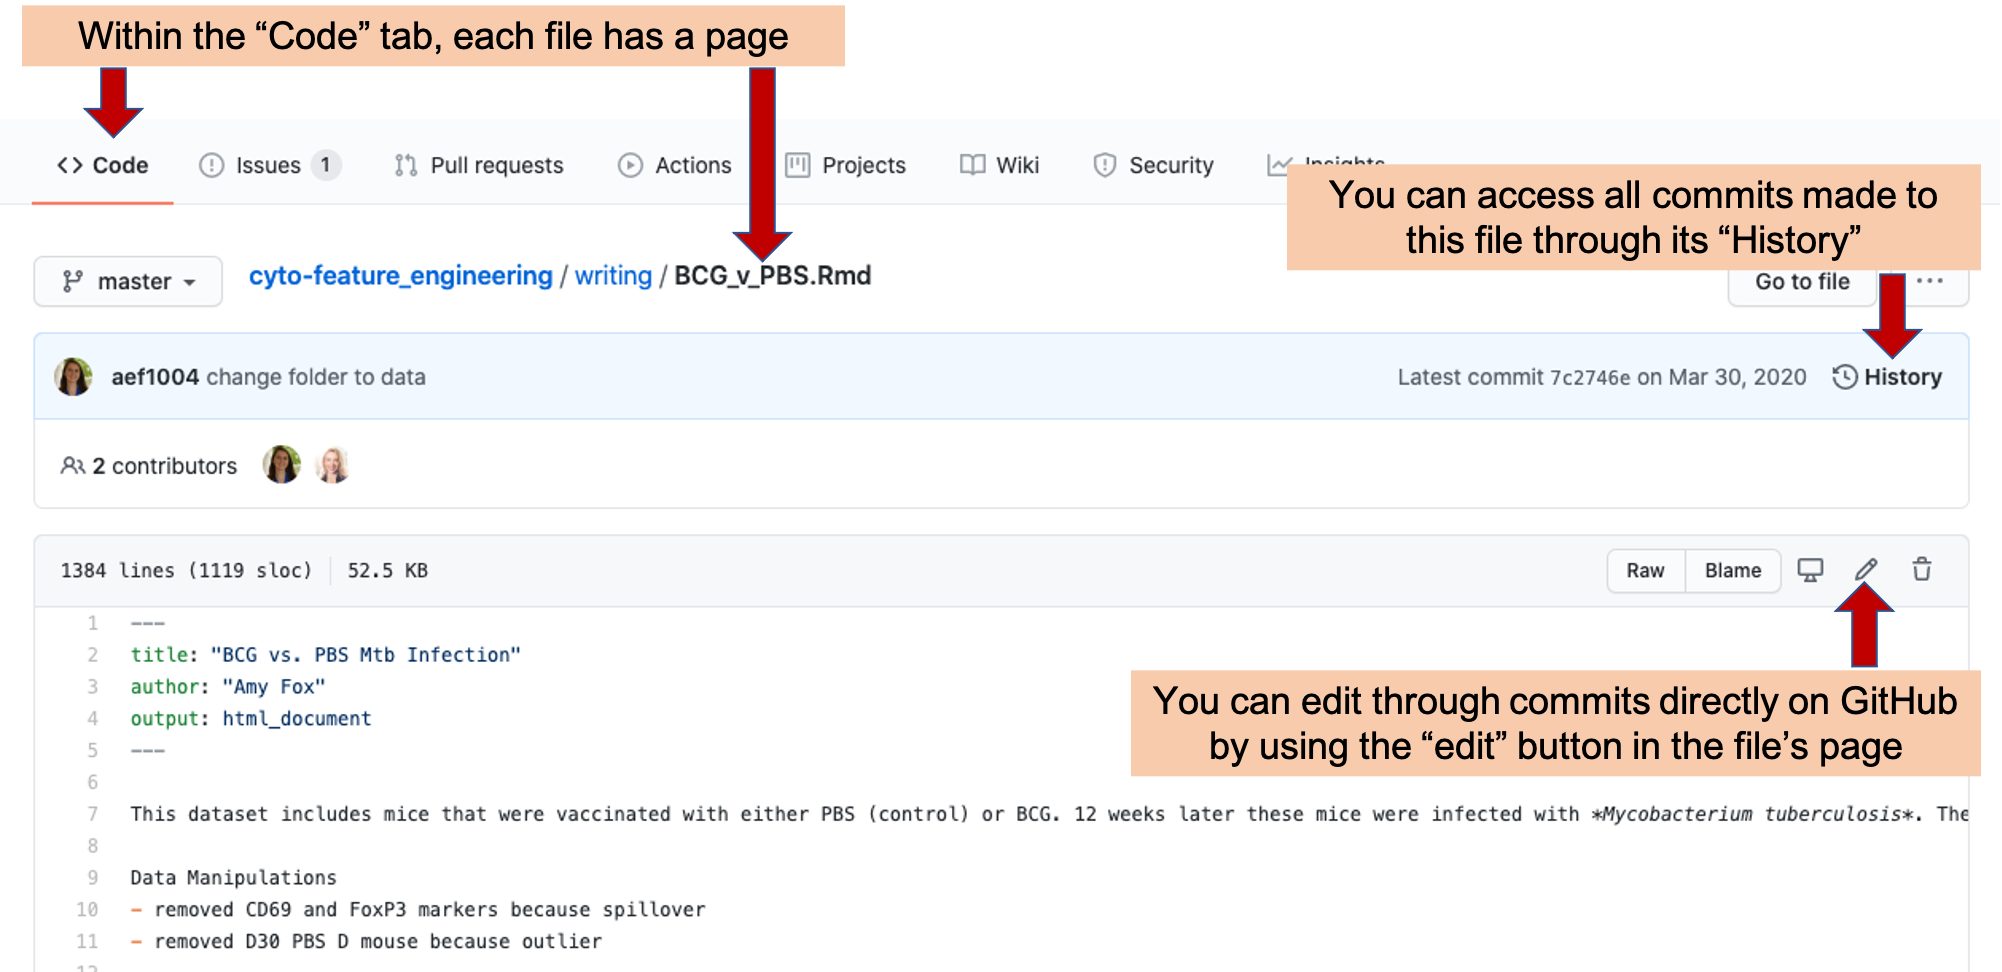
\includegraphics[width=\textwidth]{figures/github_commits1} \caption[Example of a file page within a GitHub repository]{Example of a file page within a GitHub repository. Each file in a repository has its own page. On this page, you can see the history of changes made to the file by looking at 'History'. You can also make a commit an edit directly in GitHub by clicking on the 'Edit' icon.}\label{fig:githubcommits1}
\end{figure*}

You can make changes to a file locally, on the repository copy on your own computer.
For team members who are working a lot on coding, this will likely be the primary
method they use to make commits, as this allows you to test the code locally before
you commit it.

However, it is also possible to make a commit directly on GitHub, and this may be a
useful option for team members who are not coding and would like to make small changes
to the writing files. On the file's page on GitHub, there is an ``Edit'' icon
(Figure \ref{fig:githubcommits1}). By clicking on this, you will get to a page where you
can directly edit the file (Figure \ref{fig:githubcommits2}). Once you have made your
edits, you will need to commit them, and a short description of the commit is required.
If you would like to include a longer explanation of your changes, there is space for
that, as well, when you make the commit (Figure \ref{fig:githubcommits2}).

\begin{figure*}
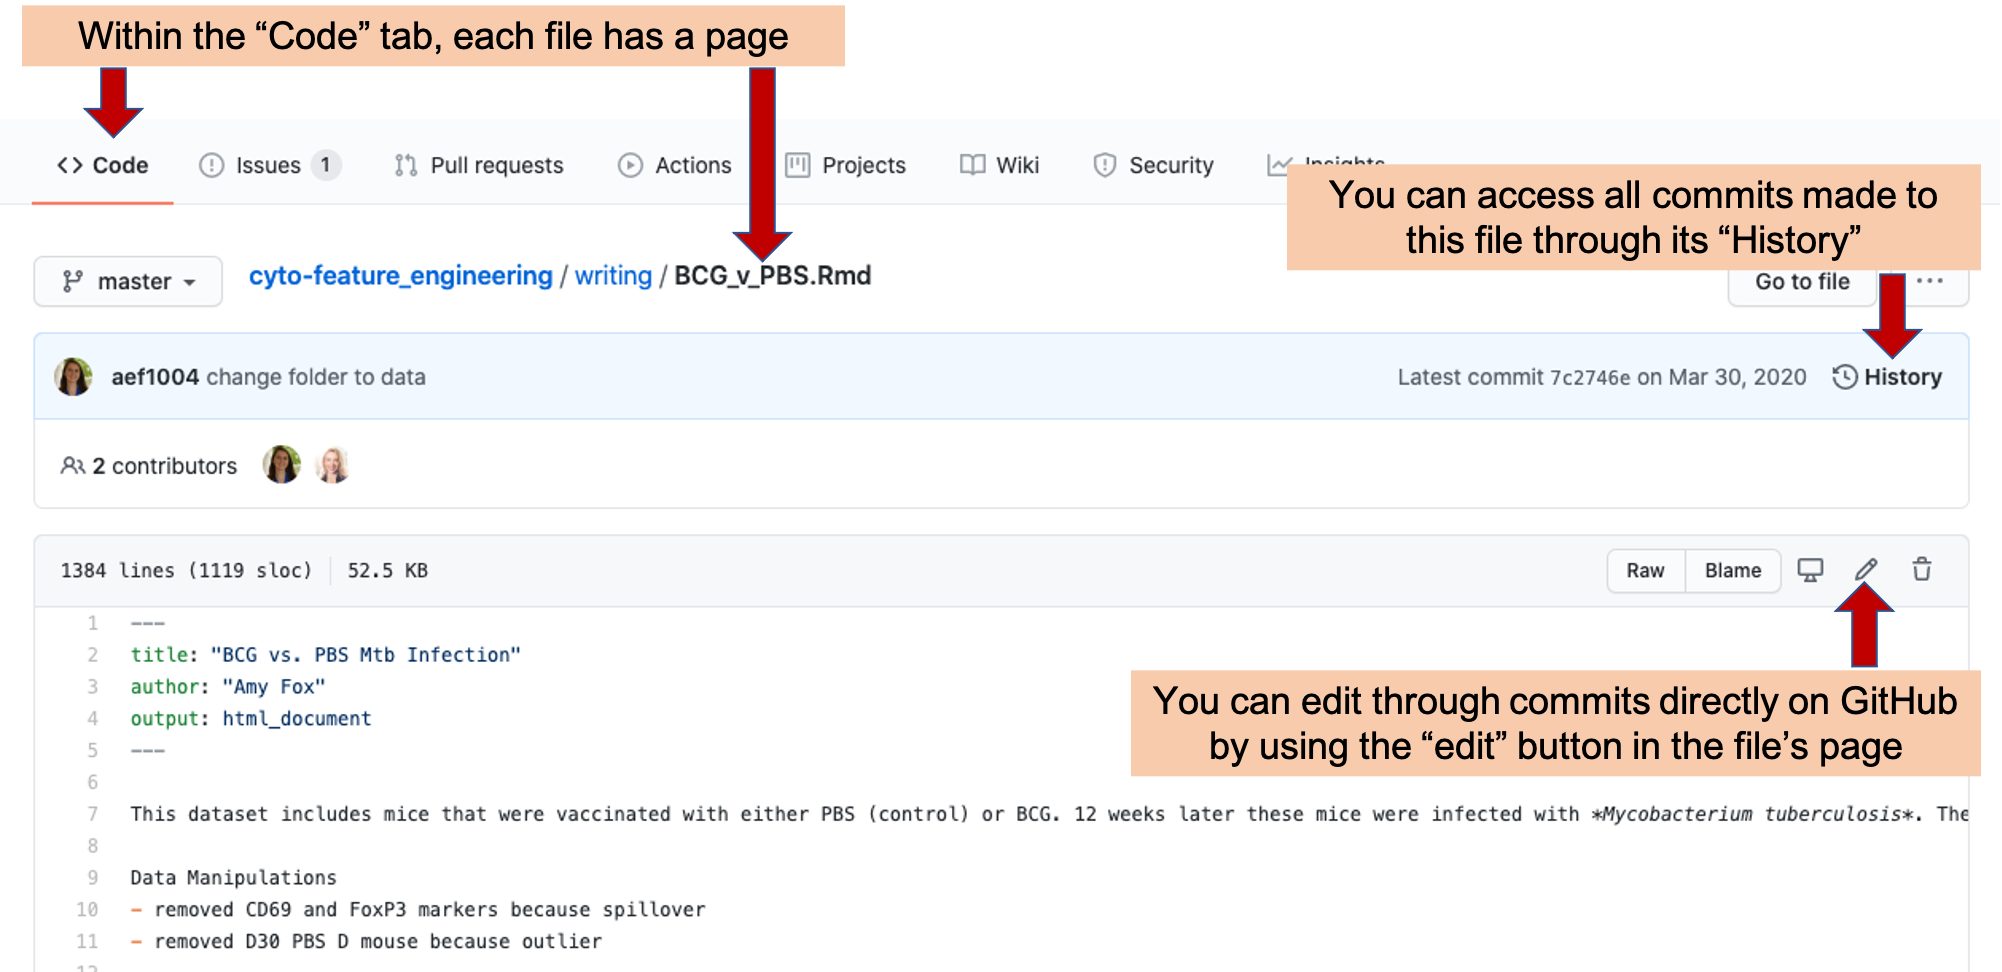
\includegraphics[width=\textwidth]{figures/github_commits1} \caption[Committing changes directly in GitHub]{Committing changes directly in GitHub. When you click on the 'Edit' button in a file's GitHub page (see previous figure), it will take you to a page where you can edit the file directly. You save the changes with a 'commit', including a commit message describing why you made the change. The change will be tagged with the message and your name.}\label{fig:githubcommits2}
\end{figure*}

You can see the full history of changes that have been made to each file in the
project (Figure \ref{fig:githubcommithistory}). Each change is tracked through
a commit, which includes markers of who made the change and a message describing
the change. Further, this history page for the file provides a line-by-line
history of when each line in the file was last changed and what that change
is---this allows you to quickly pinpoint changes in a particular part of the
file.

\begin{figure*}
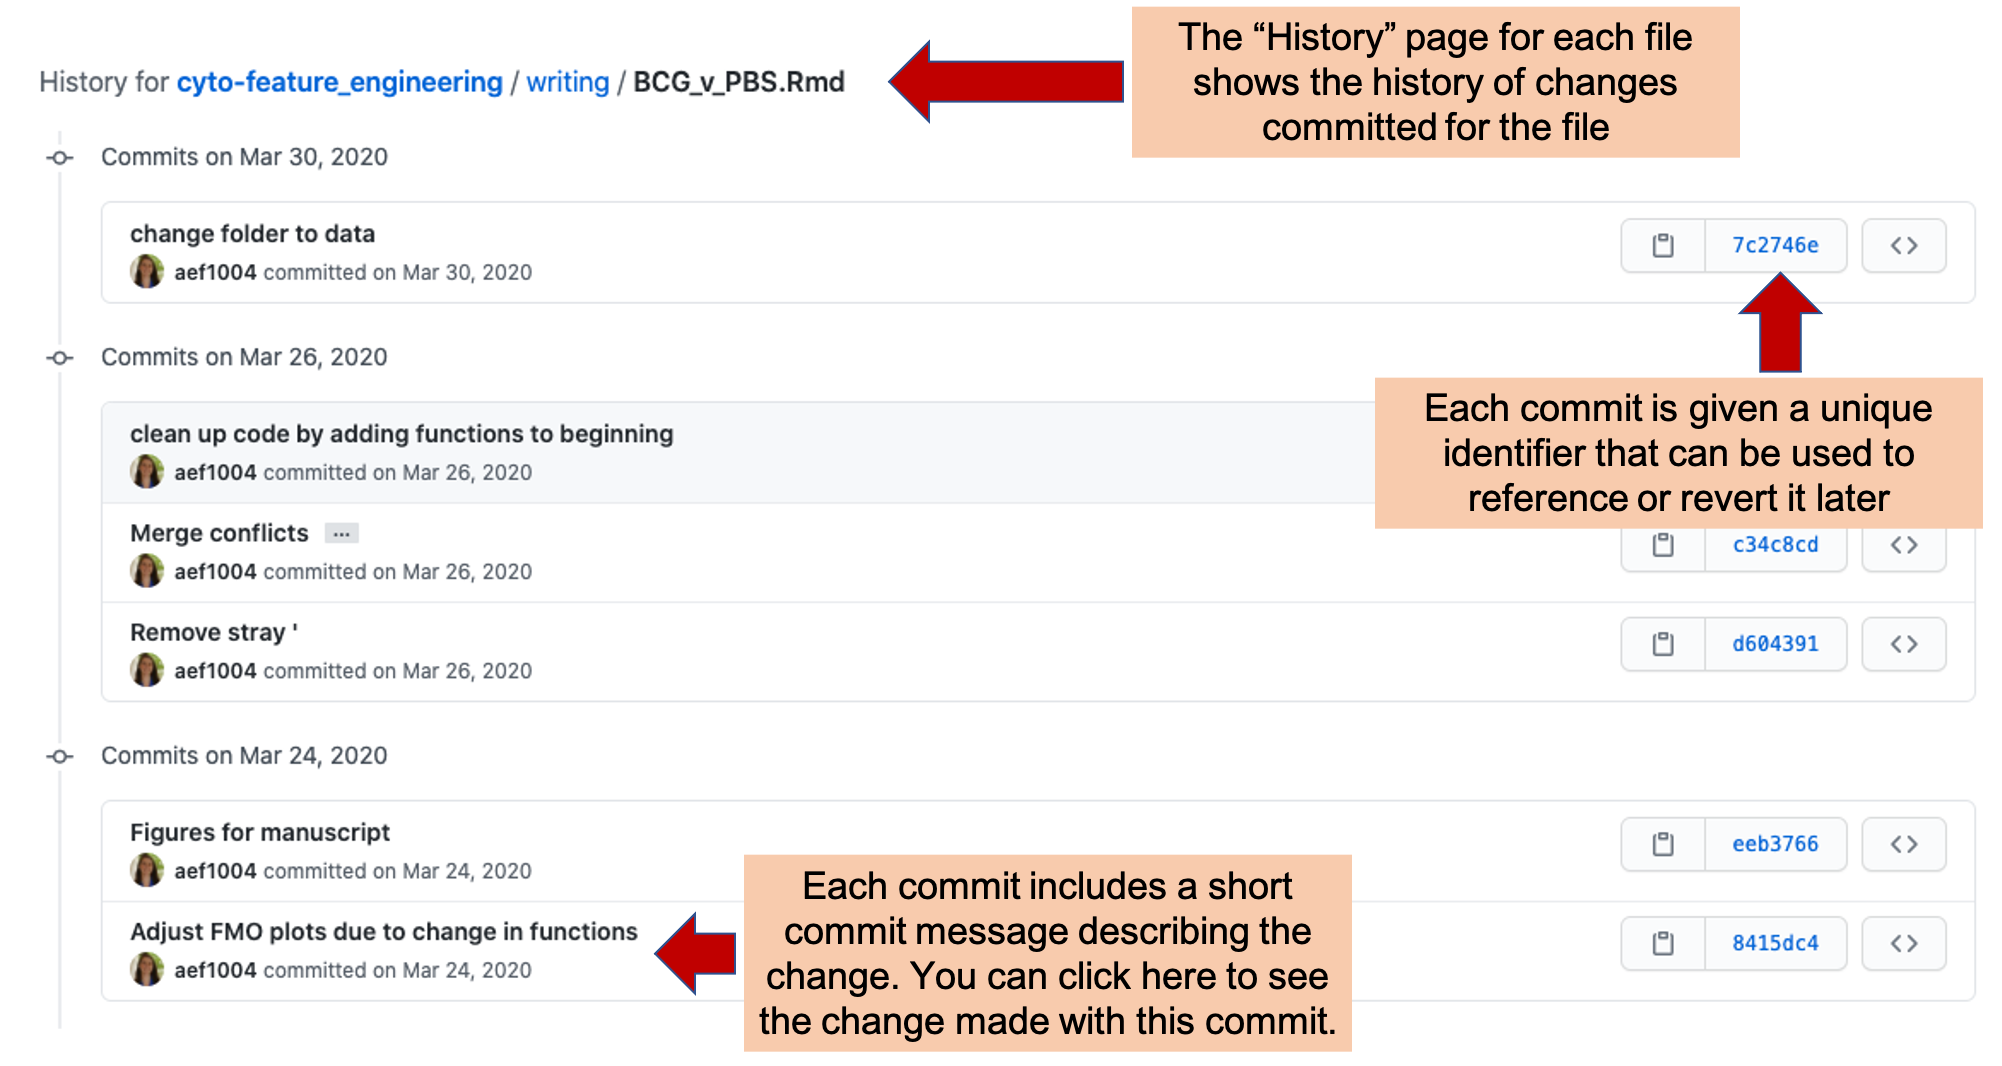
\includegraphics[width=\textwidth]{figures/github_commit_history} \caption[Commit history in GitHub]{Commit history in GitHub. Each file in a repository has a 'History' page, where you can explore each change commited for the file. Each commit has a unique identifier and commit message describing the change. You can click on the entry for any of these commits to see the changes made to the file with the commit (see next figure).}\label{fig:githubcommithistory}
\end{figure*}

If you click on one of the commits listed on a file's History page (Figure
\ref{fig:githubcommithistory}, it will take you to a page providing information
on the changes made with that commit (Figure \ref{fig:githubcommithistory2}).
This page provides a line-by-line view of each change that was made to project
files with that commit. This page includes the commit message for that commit.
If the person committing the change included a longer description or commentary
on the commit, this information will also be included on this page. Near the
commit message are listings of which team member made the commit and when it was
made. Within the body of the page, you can see the changes made with the commit.
Added lines will be highlighted in green while deleted lines are highlighted in
red. If only part of a line was changed, it will be shown twice, once in red as
its version before the commit, and once in green showing its version following
the commit.

\begin{figure*}
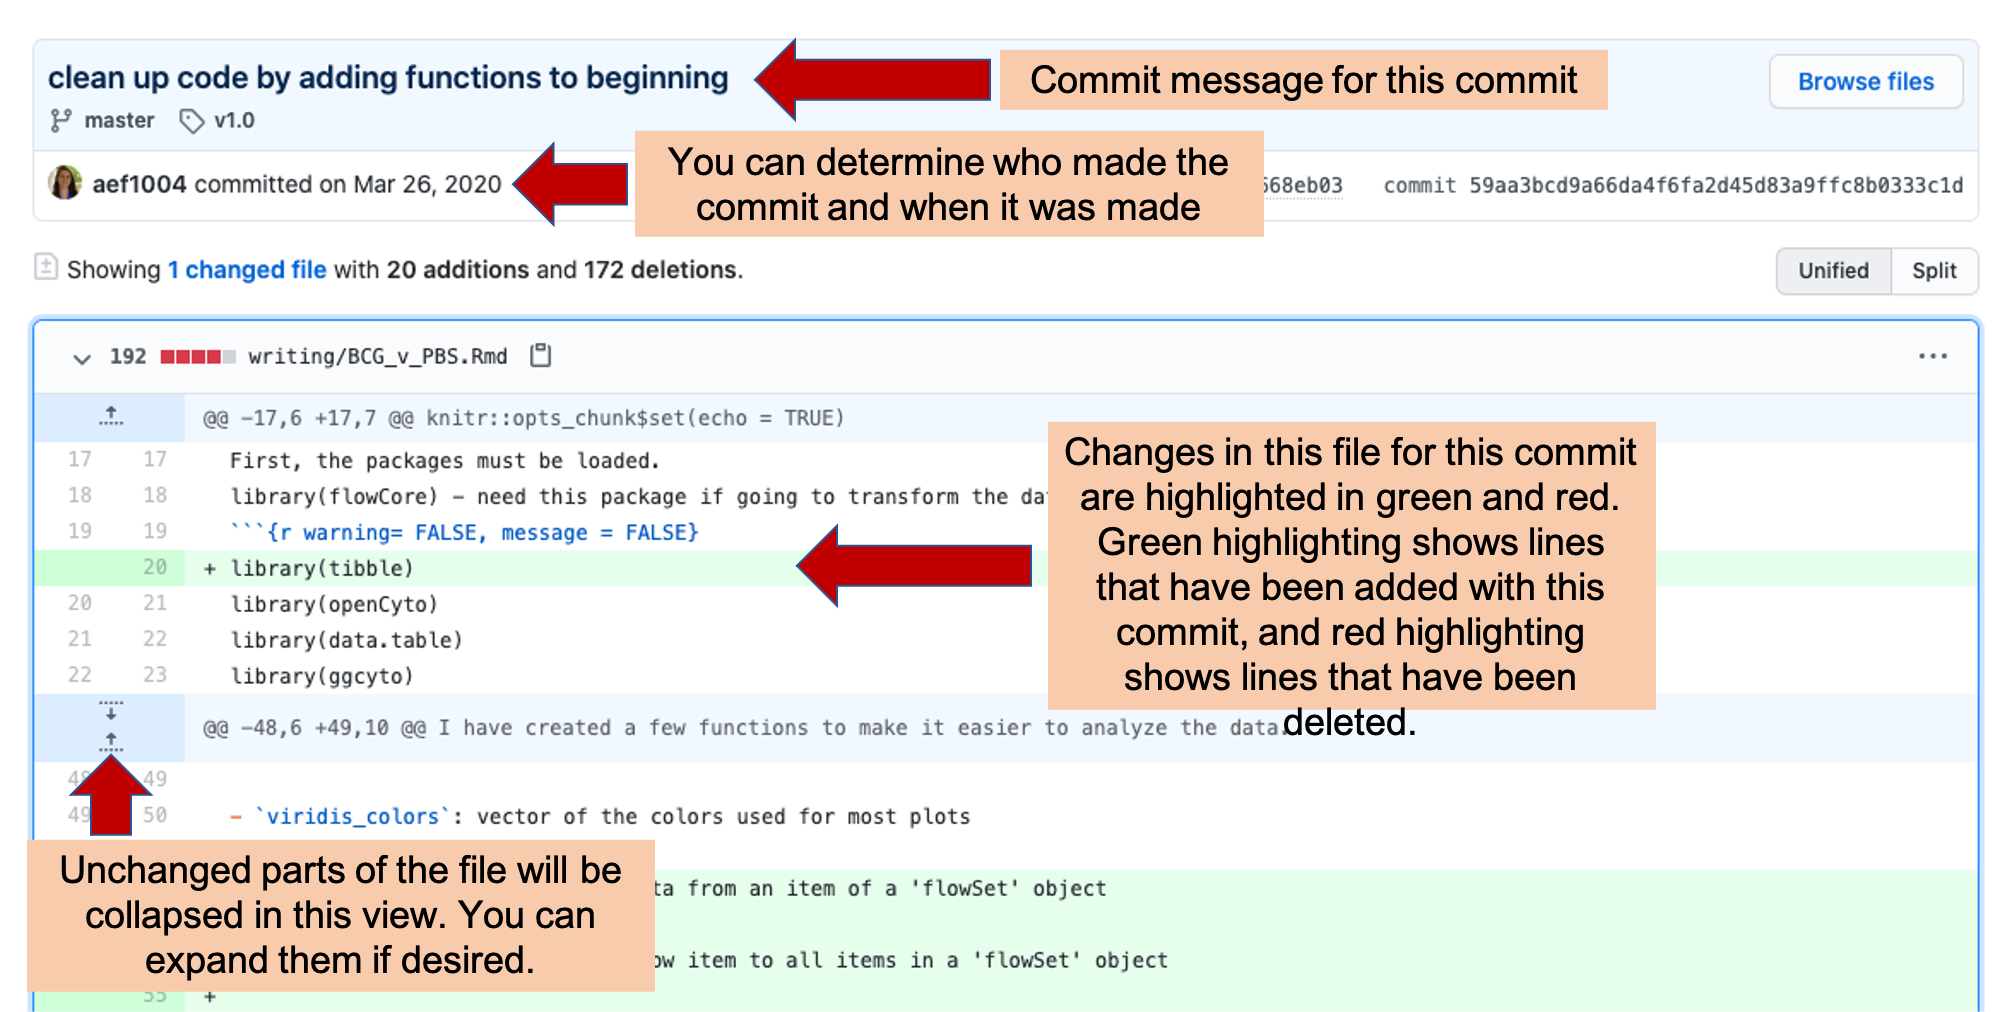
\includegraphics[width=\textwidth]{figures/github_commit_history2} \caption[Commit history in GitHub]{Commit history in GitHub. Each commit has its own page, where you can explore what changes were made with the commit, who made them, and when they were committed.}\label{fig:githubcommithistory2}
\end{figure*}

\textbf{Issues}

GitHub, as well as other version control platforms, includes functionality
that will help your team collaborate on a project. A key tool is the
``Issues'' tracker. Each repository includes this type of tracker, and it
can be easily used by all team members, whether they are comfortable
coding or not.

Figure \ref{fig:githubissues1} gives an example of \href{https://github.com/aef1004/cyto-feature_engineering/issues}{the Issues tracker page} for the
repository we are using as an example.

\begin{figure*}
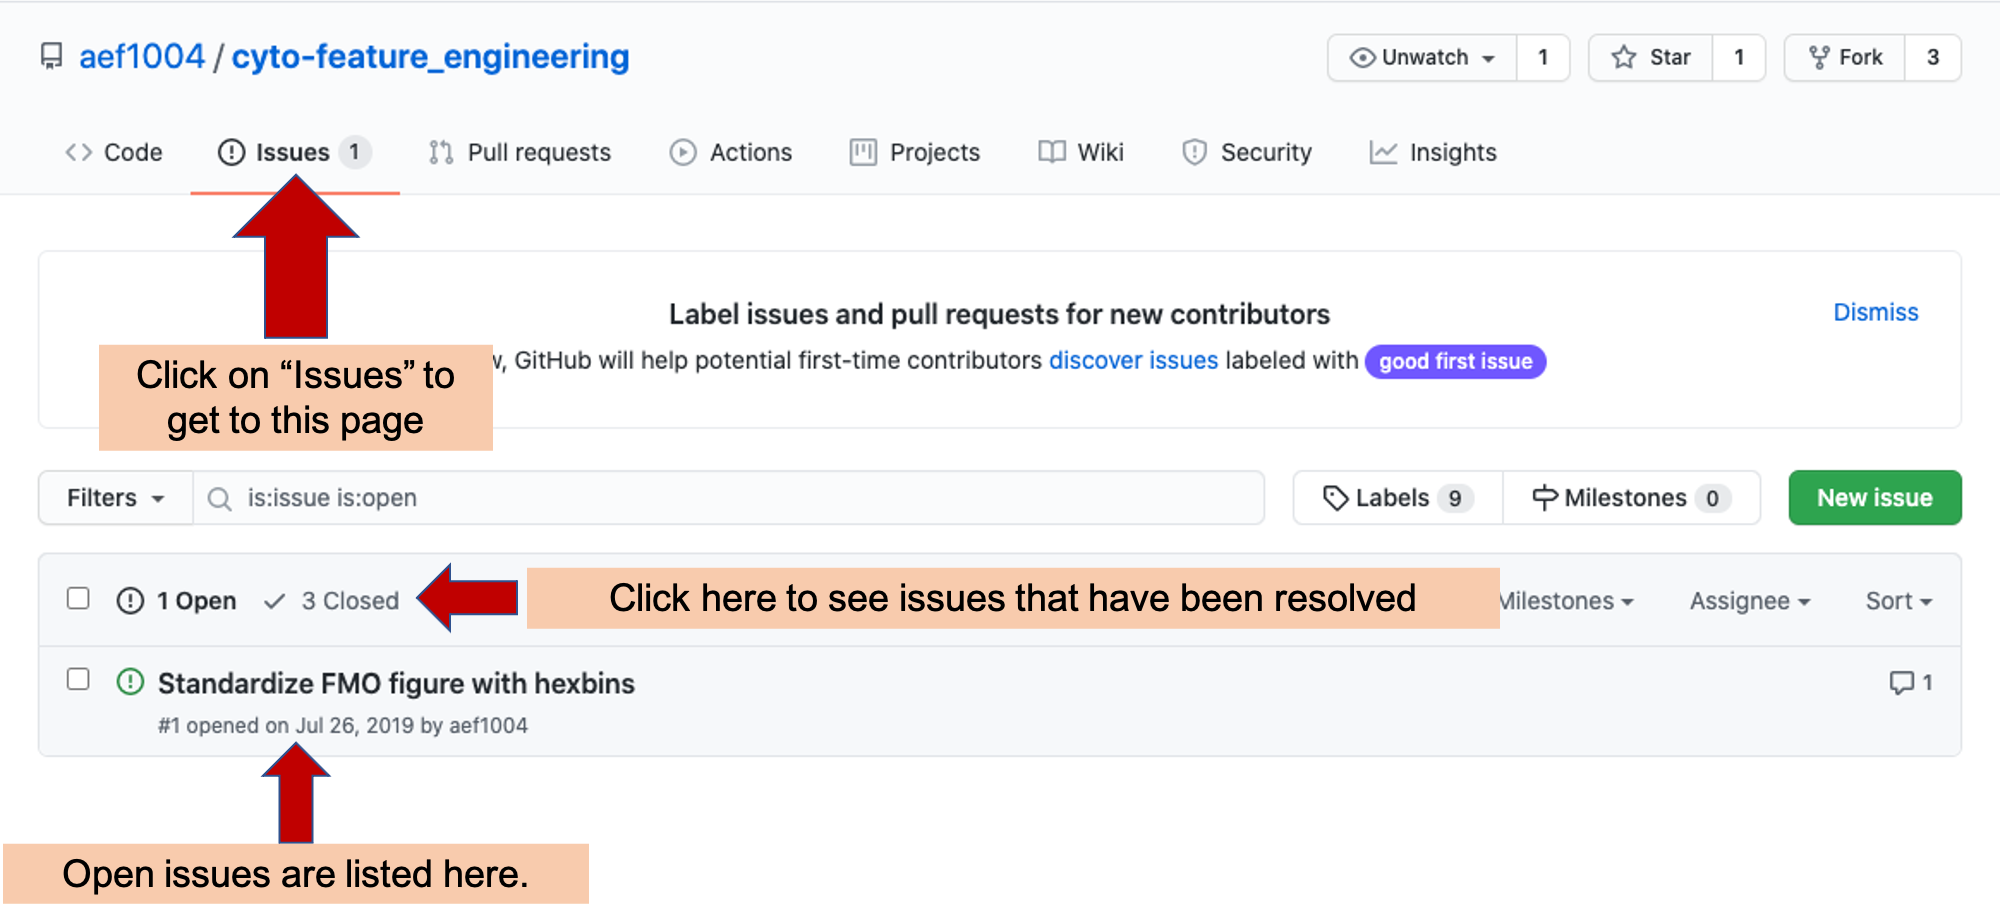
\includegraphics[width=\textwidth]{figures/github_issues} \caption[Issues tracker page for an example GitHub repository]{Issues tracker page for an example GitHub repository. Arrows highlight the tab to click to get to the Issues tracker page in a repository, as well as where to go to find open and closed Issues for the repository.}\label{fig:githubissues1}
\end{figure*}

The main Issues tracker page provides clickable links to all open issues for
the repository. You can open a new issue using the ``New Issue'' on this main
page or on the specific page of any of the repository's issues (see Figure
\ref{fig:githubissues2} for an example of this button).

\begin{figure*}
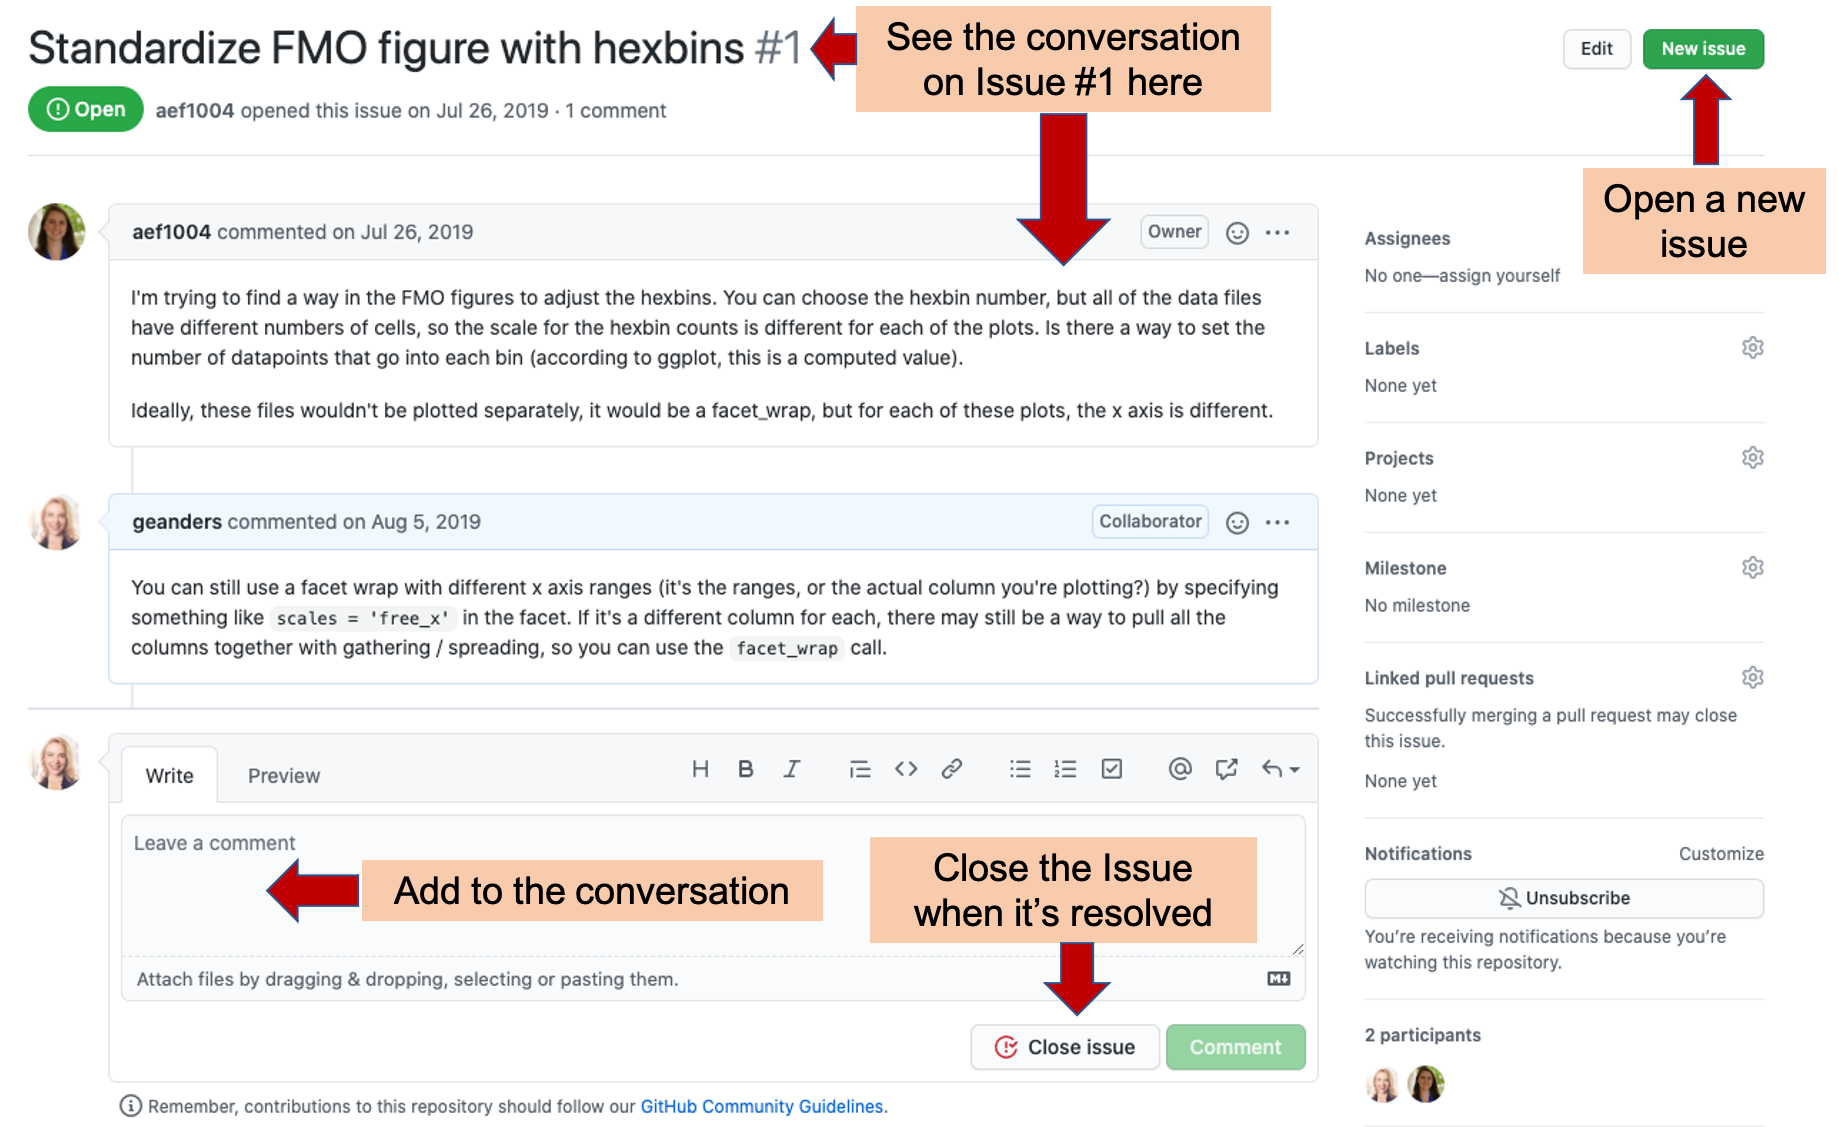
\includegraphics[width=\textwidth]{figures/github_issues2} \caption[Conversation about an Issue on Issues tracker page of an example GitHub repository]{Conversation about an Issue on Issues tracker page of an example GitHub repository. In this example, you can see how GitHub Issues trackers allow you to discuss how to resolve an issue across your team. From this page, you can read the current conversation about Issue \#1 of the repository and add your own comments. Once the Issue is resolved, you can 'Close' the Issue, which moves it off the list of active issues, but allows you to still re-read the conversation and, if necessary, re-open the issue later. You can also open a new issue from this page, using the button highlighted at the top right.}\label{fig:githubissues2}
\end{figure*}

On the page for a specific issue (e.g., Figure \ref{fig:githubissues2}), you
can have a conversation with your team to determine how to resolve the issue.
This conversation can include web links, figures, and ``To-do'' check boxes, to
help you discuss and plan how to resolve the issue. Each issue is numbered,
which allows you to track each individually as you work on the project.

Once you have resolved an issue, you can ``Close'' it. This moves the issue
from the active list into a ``Closed'' list. Each closed issue still has its
own page, where you can read through the conversation describing how it
was resolved. If you need to, you can re-open a closed issue later, if you
determine that it was not fully resolved.

\begin{figure*}
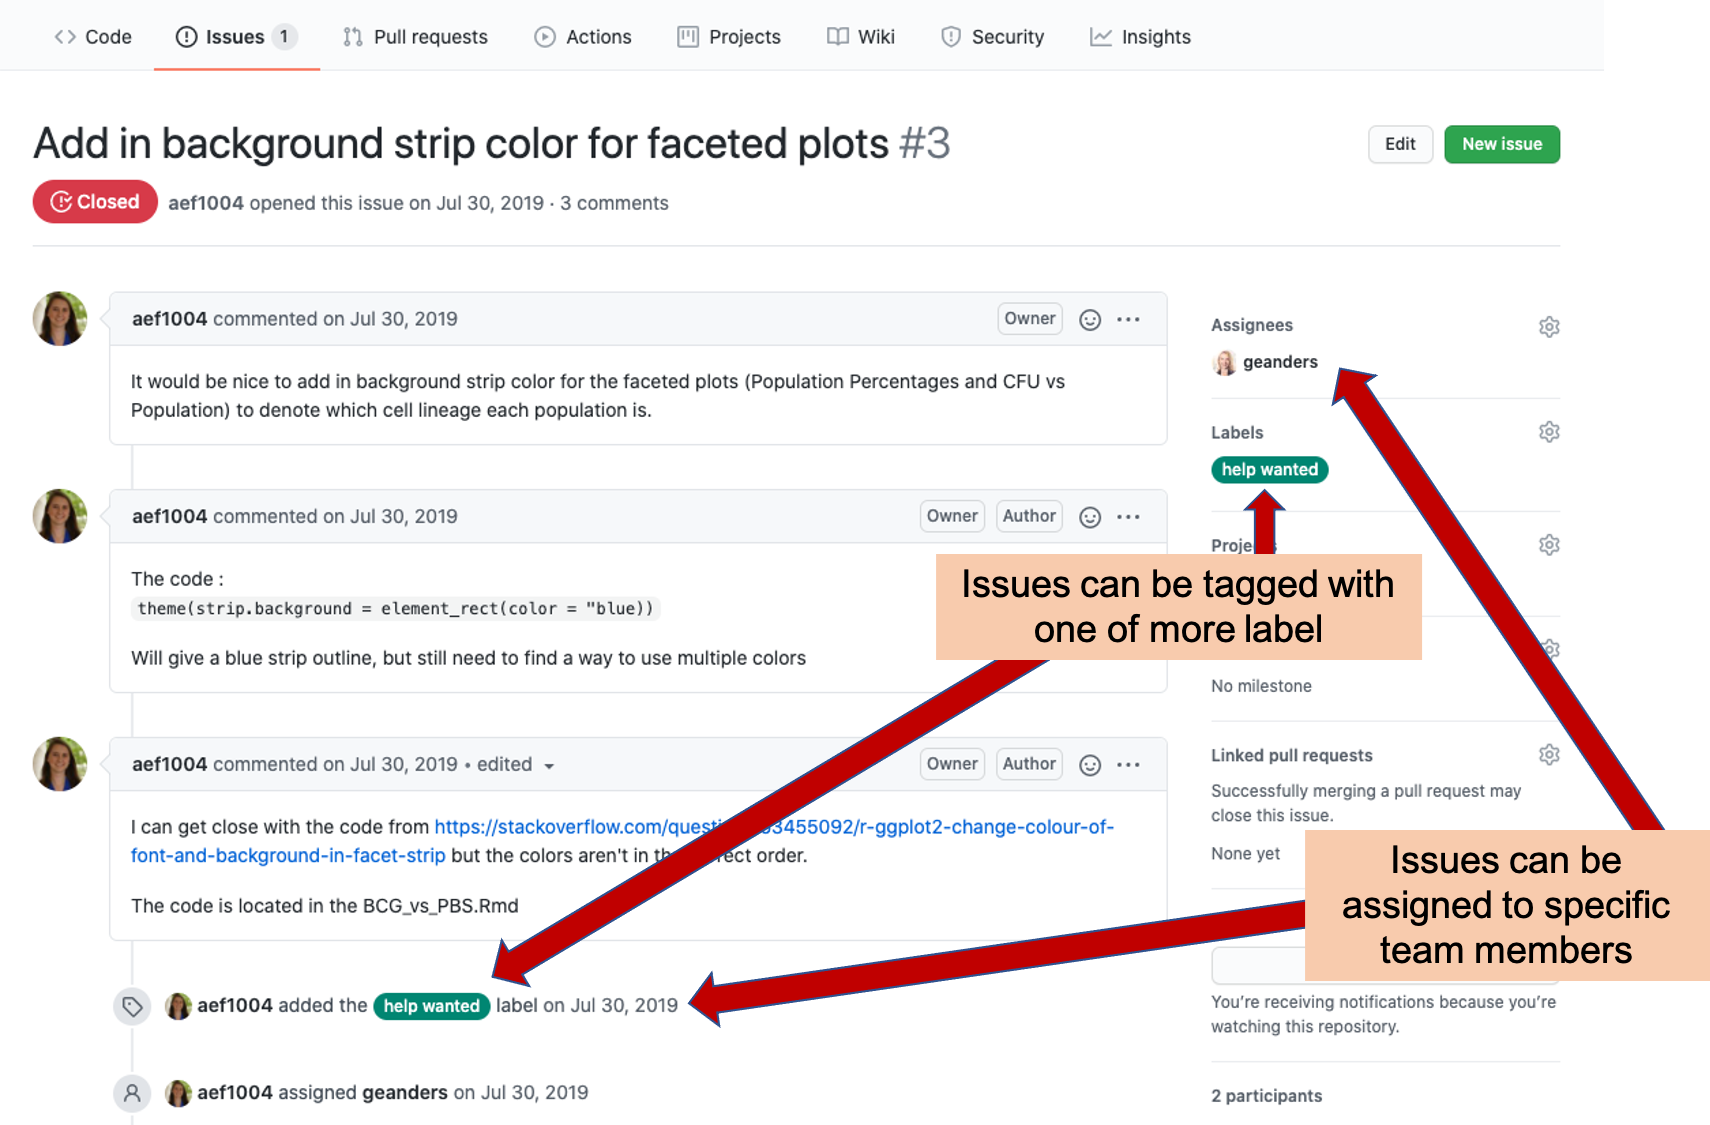
\includegraphics[width=\textwidth]{figures/github_issues3} \caption[Labeling and assigning Issues]{Labeling and assigning Issues. The GitHub Issues tracker allows you to assign each issue to one or more team members, clarifying that they will take the lead in resolving the issue. It also allows you to tag each issue with one or more labels, so you can easily navigate to issues of a specific type or identify the category of a specific issue.}\label{fig:githubissues3}
\end{figure*}

The Issues tracker page includes some more advanced functionality, as well
(Figure \ref{fig:githubissues3}). For example, you can ``assign'' an issue to one
of more team members, indicating that they are responsible for resolving that
issue. You can also tag each issue with one of more labels, allowing you to
group issues into common categories. For example, you could tag all issues that
cover questions about pre-processing the data using a ``pre-processing'' label,
and all that are related to creating figures for the final manuscript with a
``figures'' label.

\textbf{Repository access and ownership}

Repositories include functionality for inviting team members, assigning
roles, and otherwise managing access to the repository. First, a repository
can be either public or private. For a public repository, anyone will be
able to see the full contents of the repository through GitHub. You can
also set a repository to be private. In this case, the repository can only
be seen by those who have been invited to collaborate on the repository, and
only when they are logged in to their GitHub accounts. The private / public
status of a repository can be changed at any time, so if you want you can
maintain a repository for a project as private until you publish the results,
and then switch it to be public, to allow others to explore the code and data
that are linked to your published results.

You can invite team members to collaborate on a repository, as long as they
have GitHub accounts (these are free to sign up for). While public repositories
can be seen by anyone, the only people who can add to or change the contents
of the repository are people who have been invited to collaborate on the
repository. The person who creates the repository can invite other collaborators
through the ``Settings'' tab of the repository, which will have a ``Manage access''
function for the repositories maintainer. On this page, you can invite other
collaborators by searching using their GitHub ``handle'' (the short name they
chose to be identified by in GitHub). You can also change access rights, for
example, allowing some team members to be able to make major changes to the
repository---like deleting it---while others can make only smaller modifications.

\textbf{Insights}

Each GitHub repository also provides an ``Insights'' page, which lets you see who is
contributing to the project and, as well when and how much they have contributed, as
tracked by the commits they've made.

First, this page provides some repository-wide summaries, regardless of who was
contributing. The figure below shows an example of the ``Code frequency'' graph,
showing the number of additions and deletions to the code each week (here, ``code'' means
any data in the tracked files, so it would include data recorded for the project or
text written up for a project report or presentation {[}double-check that this is the
case{]}).

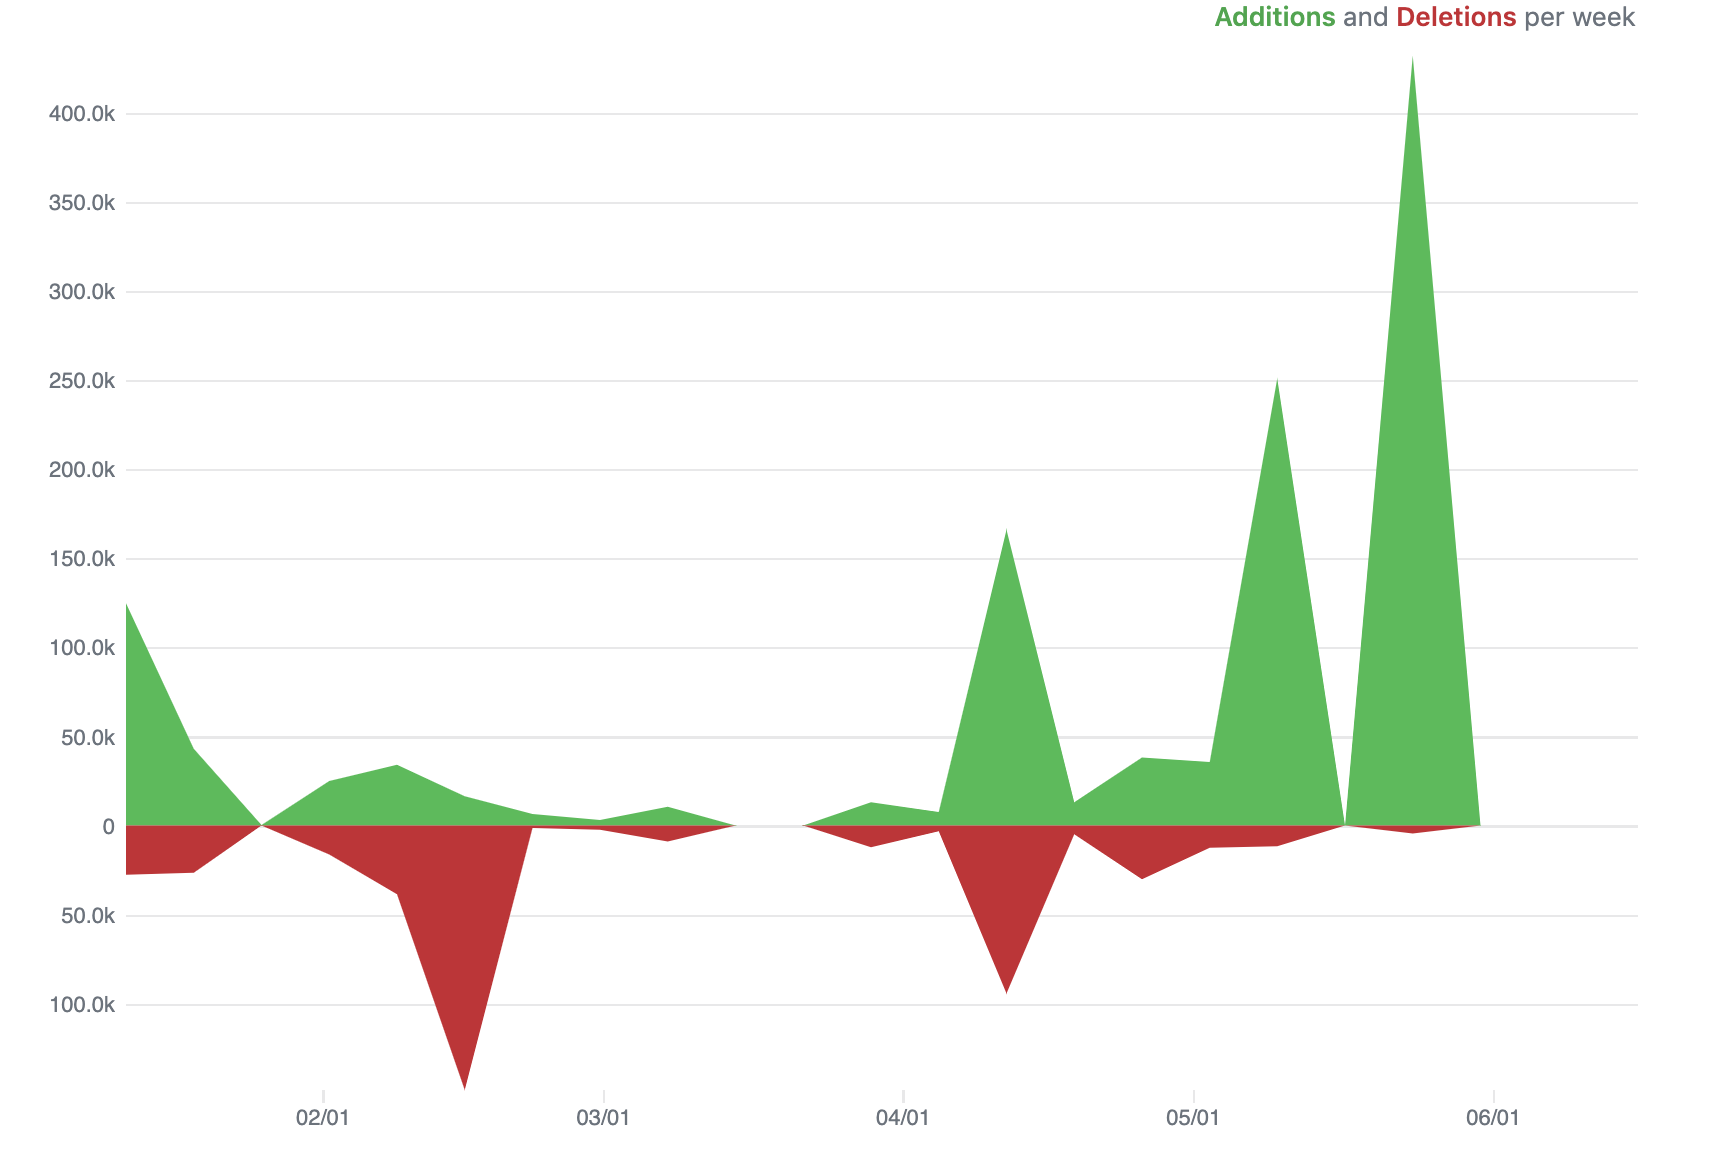
\includegraphics[width=24in]{figures/github_code_frequency}

During periods when the research team is collecting data, you would expect
a lot more additions that deletions, and you could check this plot to ensure that the
team is committing data soon after it's recorded (i.e., that there are lots of additions
on weeks with major data collection for the experiment, not several weeks after).
Periods with a lot of deletions, aren't bad, but instead likely indicate that a lot of
work is being done in editing reports and manuscripts. For example, if a paper is being
prepared for publication, you'd expect a lot of delections as the team edits it to meet
word count requirements.

The ``Insights'' page on a GitHub repository also lets you track the frequency of commits
to the project, where each commit could be something small (like fixing a typo) or
large (adding new data files for all data recorded for a timepoint for the experiment).
However, the frequency of these commits can help identify periods when the team is working
on the project. For example, the commit history graph shown below is for the GitHub
repository for a website for a spring semester course in 2020. It's clear to see the
dates when the course was in session, as well as how the project required a lot of
initial set up (shown by the number of commits early in the project period compared
to later). You can even see spring break in mid-March (the week in the middle with no
commits).

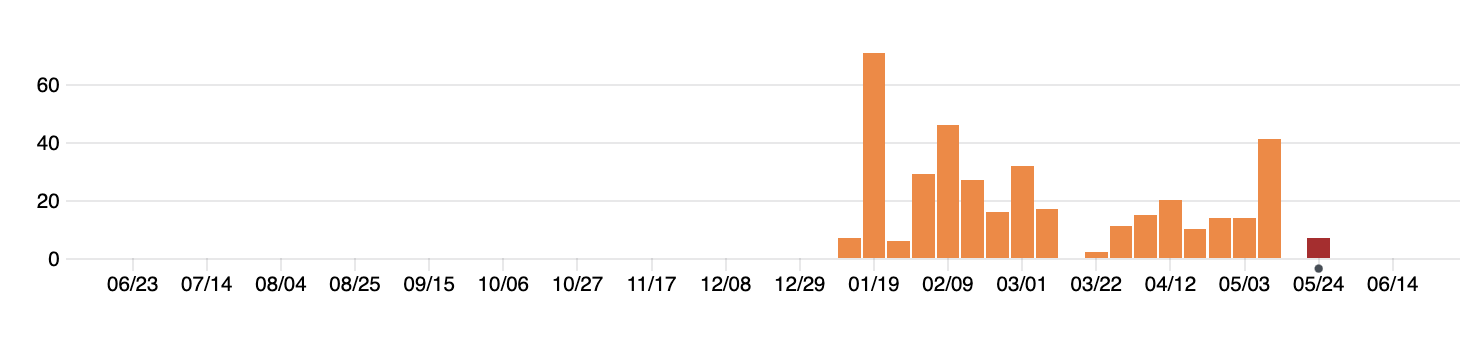
\includegraphics[width=20.53in]{figures/github_commit_frequency}

This window also allows you to track the number and timing of commits of each contributor
to the project.

\hypertarget{leveraging-git-and-github-as-a-scientist-who-programs}{%
\subsection{Leveraging git and GitHub as a scientist who programs}\label{leveraging-git-and-github-as-a-scientist-who-programs}}

To be able to leverage GitHub to manage projects and share data, you will
need to have at least one person in the research group who can set up the
initial repository. GitHub repositories can be created very easily starting
from an RStudio Project, a format for organizing project files that was
described in module {[}x{]}. In this section, we'll give some advice on how you
can use an RStudio Project to create and update a GitHub repository, and how
this can allow separate team members to maintain identical copies of the
RStudio Project on their own computers, while continually evolving files in
the project as data pre-processing, data analysis, and manuscript
preparation are done for the project. We will keep this advice limited,
as there are excellent existing resources that provide more thorough
instructions in this area, but we will introduce the methods and then
point to more thorough resources for more detail.

\begin{itemize}
\tightlist
\item
  Interfacing with RStudio
\item
  Initiating a repository and first commit
\item
  Subsequent commits and commit messages
\item
  Fixing merge conflicts when team members make concurrent changes
\item
  Using branches and forks / pull requests to try out new things
\item
  Using GitHub Actions for automation (e.g., automatic testing?)
\item
  {[}Odds and ends---.DS\_Store, \$Word\_doc{]}
\item
  More resources for learning to use git and GitHub
\end{itemize}

\begin{quote}
``Get a new repository in the directory you are working in via: \texttt{git\ init}. Ok, you
now have a revision control system in place. You might not see it, because Git stores
all its files in a directory names \texttt{.git}, where the dot means that all the usual
utilities like \texttt{ls} will take it to be hidden. You can look for it via, e.g.,
\texttt{ls\ -a} or via a show hidden files option in your favorite file manager. \ldots{}
Given that all the data about a repository is in the \texttt{.git\textbackslash{}\ subdirectory\ of\ your\ project\ directory,\ the\ analog\ to\ freeing\ a\ repository\ is\ simple:}rm -rf .git`.''
\citep{klemens201421st}
\end{quote}

\begin{quote}
``Calling \texttt{git\ commit\ -a} writes a new commit object to the repostiory based on
all the changes the index was able to track, and clears the index. Having saved your
work, you can now continue to add more. Further---and this is the real, major
benefit of revision control so far---you can delete whatever you want, confident
that it can be recovered if you need it back. Don't clutter up the code with large
blocks of commented-out obsolete routines---delete!'' \citep{klemens201421st}
\end{quote}

\begin{quote}
``Having generated a commit object, your interactions with it will mostly consist of
looking at its contents\ldots{} The key metadata is the name of the object, which is
assigned via an unpleasant but sensible naming convention: the SHA1 has, a
40-digit hexadecimal number that can be assigned to an object, in a manner that
lets us assume that no two objects will have the same hash, and that the same object
will have the same name in every copy of the repository. When you commit your files,
you'll see the first few digits of the hash on the screen\ldots{} Fortunately, you
need only as much of the hash as will uniquely identify your commit.''
\citep{klemens201421st}
\end{quote}

\hypertarget{applied-exercise-3}{%
\subsection{Applied exercise}\label{applied-exercise-3}}

\hypertarget{experimental-data-preprocessing}{%
\chapter{Experimental Data Preprocessing}\label{experimental-data-preprocessing}}

This section includes modules on:

\begin{itemize}
\tightlist
\item
  \protect\hyperlink{module12}{Module 12: Principles and benefits of scripted pre-processing of experimental data}
\item
  \protect\hyperlink{module13}{Module 13: Introduction to scripted data pre-processing in R}
\item
  \protect\hyperlink{module14}{Module 14: Simplify scripted pre-processing through R's `tidyverse' tools}
\item
  \protect\hyperlink{module15}{Module 15: Complex data types in experimental data pre-processing}
\item
  \protect\hyperlink{module16}{Module 16: Complex data types in R and Bioconductor}
\item
  \protect\hyperlink{module17}{Module 17: Example: Converting from complex to `tidy' data formats}
\item
  \protect\hyperlink{module18}{Module 18: Introduction to reproducible data pre-processing protocols}
\item
  \protect\hyperlink{module19}{Module 19: RMarkdown for creating reproducible data pre-processing protocols}
\item
  \protect\hyperlink{module20}{Module 20: Example: Creating a reproducible data pre-processing protocol}
\end{itemize}

\hypertarget{module12}{%
\section{Principles and benefits of scripted pre-processing of experimental data}\label{module12}}

The experimental data collected for biomedical research often requires
pre-processing before it can be analyzed (e.g., gating of flow cytometry data,
feature finding / quantification for mass spectrometry data). Use of
point-and-click software can limit the transparency and reproducibility of this
analysis stage and is time-consuming for repeated tasks. We will explain how
scripted pre-processing, especially using open source software, can improve
transparency and reproducibility.

\textbf{Objectives.} After this module, the trainee will be able to:

\begin{itemize}
\tightlist
\item
  Define `pre-processing' of experimental data
\item
  Describe an open source code script and explain how it can increase
  reproducibility of data pre-processing
\end{itemize}

\hypertarget{what-is-pre-processing}{%
\subsection{What is pre-processing?}\label{what-is-pre-processing}}

Some data collected through laboratory experiments is very straightforward and
requires little or no pre-processing before it's used in analysis. For example,
{[}example{]}. Other data may require some minimal pre-processing. For example, if
you plate bacteria from a sample at a variety of dilutions, you might count each
plate and determine a measure of Colony Forming Units from the set of plates
with different dilutions by deciding which dilution provides the clearest count
and then back-calculating based on its dilution to get the total number of
colony-forming units in the original sample.

This step of pre-processing data can become much more complex with data that was
collected using complex equipment, like a flow cytometer or a mass spectrometer.
In these cases, there are often steps required to extract from the machine's
readings a biologically-relevant measurement. For example, the data output from
a mass spectrometer must be processed to move from measurements of mass and
retention time to estimates of concentrations of different molecules in the
sample. If you want to compare across multiple samples, then the preprocessing
will also involve steps to align the different samples (in terms of \ldots), as
well as to standardize the measurements for each sample, to make the
measurements from the different samples comparable. For data collected from a
flow cytometer, preprocessing may include steps to disentangle the florescence
from different markers to ensure that the read for one marker isn't inflated by
spillover florescence from a different marker.

\hypertarget{approaches-to-simple-preprocessing-tasks}{%
\subsection{Approaches to simple preprocessing tasks}\label{approaches-to-simple-preprocessing-tasks}}

There are several approaches for tackling this type of data preprocessing, to
get from the data that you initial observe (or that is measured by a piece of
laboratory equipment) to meaningful biological measurements that can be analyzed
and presented to inform explorations of a scientific hypothesis. While there are
a number of approaches that don't involve writing code scripts for this
preprocessing, there are some large advantages to scripting preprocessing any
time you are preprocessing experimental data prior to including it in figures or
further analysis. In this section, we'll describe some common non-scripted
approaches and discuss the advantages that would be brought by instead using a
code script. In the next module, we'll walk through an example of how scripts
for preprocessing can be created and applied in laboratory research.

In cases where the pre-processing is mathematically straightforward and the
dataset is relatively small, many researchers do the preprocessing by hand in a
laboratory notebook or through an equation or macro embedded in a spreadsheet.
For example, if you have plated samples at different dilutions and are trying to
calculate from these the CFUs in the original sample, this calculation is simple
enough that it could be done by hand. However, there are advantages to instead
writing a code script to do this simple preprocessing.

When you write a script to do a task with data, it is like writing a recipe that
can be applied again and again. By writing a script, you encode the process a
single time, so you can take the time to check and recheck to make sure that
you've encoded the process correctly. This helps in avoiding small errors when
you do the preprocessing---if you are punching numbers into a calculator over
and over, it's easy to mistype a number or forget a step every now and then,
while the code will ensure that the same process is run every time and that it
faithfully uses the numbers saved in the data for each step, rather than relying
on a person correctly entering each number in the calculation.

Scripts can be used across projects, as well, and so they can ensure consistency
in the calculation across projects. If different people do the calculation in
the lab for different projects or experiments, and they are doing the
calculations by hand, they might each do the calculation slightly differently,
even if it's only in small details like how they report rounded numbers. A
script will do the exact same thing every time it is applied. You can even share
your script with colleagues at other labs, if you want to ensure that your data
preprocessing is comparable for experiments conducted in different research
groups, and many scientific journals will allow supplemental material with
code used for data preprocessing and analysis, or links within the manuscript
to a repository of this code posted online.

There are also gains in efficiency when you use a script. For small
pre-processing steps, these might seem small for each experiment, and certainly
when you first write the script, it will likely take longer to write and test
the script than it would to just do the calculation by hand (even more if
you're just starting to learn how to write code scripts). However, since the
script can be applied again and again, with very little extra work to apply it
to new data, you'll save yourself time in the future, and over a lot of
experiments and projects, this can add up. This makes it particularly useful to
write scripts for preprocessing tasks that you find yourself doing again and
again in the lab.

\hypertarget{approaches-to-more-complex-preprocessing-tasks}{%
\subsection{Approaches to more complex preprocessing tasks}\label{approaches-to-more-complex-preprocessing-tasks}}

Other preprocessing tasks can be much more complex, particularly those that need
to conduct a number of steps to extract biologically meaningful measurements
from the measurements made by a complex piece of laboratory equipment, as well
as steps to make sure these measurements can be meaningfully compared across
samples.

For these more complex tasks, the equipment manufacturer will often provide
software that can be used for the preprocessing. This software might conduct
some steps using defaults, and others based on the user's specifications. These
are often provided through ``GUIs'' (graphical user interfaces), where the user
does a series of point-and-click steps to process the data. In some software,
this series of point-and-click steps is recorded as the user does them, so that
these steps can be ``re-run'' later or on a different dataset.

For many types of biological data, including output from equipment like flow
cytometers and mass spectrometers, open-source software has been developed
that can be used for this preprocessing. Often, the most cutting edge methods
for data preprocessing are first available through open-source software packages,
if the methods are developed by researchers rather than by the companies, and
often many of the algorithms that are made available through the equipment
manufacturer's proprietary software are encoded versions of an algorithm
first shared by researchers as open-source software.

It can take a while to develop a code script for preprocessing the raw data from
a piece of complex equipment like a mass spectrometer. However, the process of
developing this script requires a thoughtful consideration of the steps of
preprocessing, and so this is often time well-spent. Again, this initial time
investment will pay off later, as the script can then be efficiently applied to
future data you collect from the equipment, saving you time in pointing and
clicking through the GUI software. Further, it's easier to teach someone else
how to conduct the preprocessing that you've done, and apply it to future
experiments, because the script serves as a recipe.

When you conduct data preprocessing in a script, this also gives you access to
all the other tools in the scripting language. For example, as you work through
preprocessing steps for a dataset, if you are doing it through an R script, you
can use any of the many visualization tools that are available through R. By
contrast, in GUI software, you are restricted to the visualization and other
tools included in that particular set of software, and those software developers
may not have thought of something that you'd like to do. Open-source scripting
languages like R, Python, and Julia include a huge variety of tools, and once
you have loaded your data in any of these platforms, you can use any of these
tools.

If you have developed a script for preprocessing your raw data, it also becomes
much easier to see how changes in choices in preprocessing might influence your
final results. It can be tricky to guess whether your final results are sensitive,
for example, to what choice you make for a particular tranform for part of your
data, or in how you standardize data in one sample to make different samples
easier to compare. If the preprocessing is in a script, then you can test making
these changes and running all preprocessing and analysis scripts, to see if it
makes a difference in the final conclusions. If it does, then it helps you
identify parts of preprocessing that need to be deeply thought through for the
type of data you're collecting, and you may want to explore the documentation on
that particular step of preprocessing to determine what choice is best for your
data, rather than relying on defaults.

\hypertarget{scripting-preprocessing-tasks}{%
\subsection{Scripting preprocessing tasks}\label{scripting-preprocessing-tasks}}

Code scripts can be developed for any open-source scripting languages, including
Python, R, and Julia. These can be embedded in or called from literate programming
documents, like RMarkdown and Julia, which are described in other modules. The
word ``script'' is a good one here---it really is as if you are providing the script
for a play. In an interactive mode, you can send requests to run in the programming
language step by step using a console, while in a script you provide the whole list
of all of your ``lines'' in that conversation, and the programming language will run
them all in order without you needing to interact from the console.

For preprocessing the data, the script will have a few predictible parts. First,
you'll need to read the data in. There are different functions that can be used
to read in data from different file formats. For example, data that is stored in
an Excel spreadsheet can be loaded into R using functions in a package called
\texttt{readxl}. Data that is stored in a plain-text delimited format (like a csv file)
can be loaded into R using functions in the \texttt{readr} package.

When preprocessing data from complex equipment, you can determine how to read the
data into R by investigating the file type that is output by the equipment.
Fortunately, many types of scientific equipment follow standardized file formats.
This means that open-source developers can develop a single package that can
load data from equipment from multiple manufacturers. For example, flow cytometry
data is often stored in {[}file format{]}. Other biological datasets use file
formats that are appropriate for very large datasets and that allow R to work
with parts of the data at a time, without loading the full data in. {[}netCDF?{]}
In these cases, the first step in a script might not be to load in all the data,
but rather to provide R with a connection to the larger datafile, so it can
pull in data as it needs it.

Once the data is loaded or linked in the script, the script can proceed through
steps required to preprocess this data. These steps will often depend on the type
of data, especially the methods and equipment used to collect it. For example, for
mass spectrometry data, these steps will include \ldots{} . For flow cytometry data,
these steps would include \ldots{} .

The functions for doing these steps will often come from extensions that
different researchers have made for R. Base R is a simpler collection of data
processing and statistics tools, but the open-source framework of R has allowed
users to make and share their own extensions. In R, these are often referred to
as ``packages''. Many of these are shared through the Comprehensive R Archive
Network (CRAN), and packages on CRAN can be directly installed using the
\texttt{install.packages} function in R, along with the package's names. While CRAN
is the common spot for sharing general-purpose packages, there is a specialized
repository that is used for many genomics and other biology-related R packages
called Bioconductor. These packages can also be easily installed through a call
in R, but in this case it requires an installation function from the \texttt{BiocManager}
package. Many of the functions that are useful for preprocessing biological
data from laboratory experiments are available through Bioconductor.

Table {[}x{]} includes some of the primary R packages on Bioconductor that can be
used in preprocessing different types of biological data. There are often
multiple choices, developed by different research groups, but this list provides
a starting point of several of the standard choices that you may want to
consider as you start developing code.

Much of the initial preprocessing might use very specific functions that are
tailored to the format that the data takes once it is loaded. Later in the
script, there will often be a transfer to using more general-purpose tools in
that coding language. For example, once data is stored in a ``dataframe'' format
in R, it can be processed using a powerful set of general purpose tools
collected in a suite of packages called the ``tidyverse''. This set of packages
includes functions for filtering to specific subsets of the data, merging
separate datasets, adding new measurements for each observation that are
functions of the initial measurements, summarizing, and visualizing. The
tidyverse suite of R tools is very popular in general R use and is widely
taught, including through numerous free online resources. By moving from
specific tools to these more general tools as soon as possible in the script, a
researcher can focus his or her time in learning these general purpose tools
well, as these can be widely applied across many types of data.

By the end of the script, data will be in a format that has extracted
biologically relevant measurements. Ideally, this data will be in a general
purpose format, like a dataframe, to make it easier to work with using general
purpose tools in the scripting language when the data is used in further data
analysis or to create figures for reports, papers, and presentations. Often, you
will want to save a version of this preprocessed version of the data in your
project files, and so the last step of the script might be to write out the
cleaned data in a file that can be loaded in later scripts for analysis and
visualization. This is especially useful if these data preprocessing steps are
time consuming, as is often the case for the large raw datasets output by
laboratory equipment like flow cytometers and mass spectrometers.

Figure {[}x{]} gives an example of a data preprocessing script, highlighting these
different common areas that often show up in these scripts.

{[}Some data may be incorporated into the preprocessing by downloading it from
databases or other online sources. These data downloads can be automated and
recorded by using scripted code for the download in many cases, as long as the
database or online source offers web services or another API for this type of
scripted data access. In this case, you can incorporate the script in a
RMarkdown document to record the date the data was downloaded, as well as the
code used to download it. R is able to run system calls, and one of these
will provide the current date, so this can be included in an RMarkdown file
to record the date the file is run. Further, there may be a call that can
be made to the online data source's API that returns the working version of
the database or source, and if so this can also be included in the RMarkdown
code used to access the data.{]}

RMarkdown files can be used to combine both code and more manual document
(for example, a record of which collaborator provided each type of data file).
While traditionally this more manual documentation was recommended to be
recorded in plain-text README files in a project's directory and subdirectories
\citep{buffalo2015bioinformatics}, RMarkdown files provide some advantages over
this traditional approach. First, RMarkdown files are themselves in plain
text, and so they offer the advantages of simple plain text documentation
files (e.g., ones never rendered to another format) in terms of being able
to use script-based tools to search them. Further, they can be rendered into
attractive formatted documents that may be easier to share with project
team members who do not code.

{[}Example of a function: recipe for making a vinaigrette. There will be a
``basic'' way that the function can run, which uses its default parameters.
However, you can also specify and customize certain inputs (for example,
using walnut oil instead of olive oil, or adding mustard) to tweak the
recipe in slight ways each time you use it, and to get customized outputs.{]}

{[}History of the mouse---enable GUIs, before everything was from the terminal.{]}

\hypertarget{potential-quotes}{%
\subsection{Potential quotes}\label{potential-quotes}}

\begin{quote}
For bioinformatics, ``all too often the software is developed without
thought toward future interoperability with other software products. As a
result, the bioinformatics software landscape is currently characterized
by fragmentation and silos, in which each research group develops and uses
only the tools created within their lab.'' \citep{barga2011bioinformatics}
\end{quote}

\begin{quote}
``The group also noted the lack of agility. Although they may be aware of
a new or better algorithm they cannot easily integrate it into their
analysis pipelines given the lack of standards across both data formats
and tools. It typically requires a complete rewrite of the code in order
to take advntge of a new technique or algorithm, requiring time and often
funding to hire developers.'' \citep{barga2011bioinformatics}
\end{quote}

\begin{quote}
``The benefit of working with a programming language is that you have the code in
a file. This means that you can easily reuse that code. If the code has
parameters it can even be applied to problems that follow a similar pattern.''
\citep{janssens2014data}
\end{quote}

\begin{quote}
``Data exploration in spreadsheet software is typically conducted via menus and
dialog boxes, which leaves no record of the steps taken.'' \citep{murrell2009introduction}
\end{quote}

\begin{quote}
``One reason Unix developers have been cool toward GUI interfaces is that, in their
designers' haste to make them `user-friendly' each one often becomes frustratingly
opaque to anyone who has to solve user problems---or, indeed, interact with it anywhere
outside the narrow range predicted by the user-interface designer.'' \citep{raymond2003art}
\end{quote}

\begin{quote}
``Many operating systems touted as more `modern' or `user friendly' than Unix achieve their
surface glossiness by locking users and developers into one interface policy, and offer an
application-programming interface that for all its elaborateness is rather narrow and rigid.
On such systems, tasks the designers have anticipated are very easy---but tasks they have
not anticipated are often impossible or at best extremely painful. Unix, on the other hand, has
flexibility in depth. The many ways Unix provides to glue together programs means that components
of its basic toolkit can be combined to produce useful effects that the designers of the individual
toolkit parts never anticipated.'' \citep{raymond2003art}
\end{quote}

\begin{quote}
``The good news is that a computer is a general-purpose machine, capable of performing
any computation. Although it only has a few kinds of instructions to work with, it can
do them blazingly fast, and it can largely control its own operation. The bad news is
that it doesn't do anything itself unless someone tells it what to do, in excruciating
detail. A computer is the ultimate sorcere's apprentice, able to follow instructions
tirelessly and without error, but requiring painstaking accuracy in the
specification of what to do.'' \citep{kernighan2011d}
\end{quote}

\begin{quote}
``\emph{Software} is the general term for sequences of instructions that make a computer
do something useful. It's `soft' in contrast with `hard' hardware, because it's
intangible, not easy to put your hands on. Hardware is quite tangible: if you drop
a computer on your foot, you'll notice. Not true for software.'' \citep{kernighan2011d}
\end{quote}

\begin{quote}
``Modern system increasingly use general purpose hardware---a processor, some memory,
and connections to the environment---and create specific behaviors by software. The
conventional wisdom is that software is cheaper, more flexible, and easier to change than
hardware is (especially once some device has left the factory).'' \citep{kernighan2011d}
\end{quote}

\begin{quote}
``An algorithm is a precise and unambiguous recipe. It's expressed in terms of a fixed
set of basic operations whose meanings are completely known and specified; it spells out
a sequence of steps using those operations, with all possible situations covered; it's
guaranteed to stop eventually. On the other hand, a \emph{program} is the opposite of
abstract---it's a concrete statement of the steps that a real computer must perform to
accomplish a task. The distinction between an algorithm and a program is like the difference
between a blueprint and a building; one is an idealization and the other is the real thing.''
\citep{kernighan2011d}
\end{quote}

\begin{quote}
``One way to view a program is as one or more algorithms expressed in a form that a computer
can process directly. A program has to worry about practical problems like inadequate memory,
limited processor speed, invalid and even malicious input data, faulty hardware, broken
network connections, and (in the background and often exacerbating the other problems)
human frailty. So if an algorithm is an idealized recipe, a program is the instructions for
a cooking robot preparing a month of meals for an army while under enemy attack.'' \citep{kernighan2011d}
\end{quote}

\begin{quote}
``During the late 1950s and early 1960s, another step was taken towards getting the
computer to do more for programmers, arguably the most important step in the history of
programming. This was the development of `high-level' programming languages that were
independent of any particular CPU architecture. High-level languages make it possible to
express computations in terms that are closer to the way a person might express them.''
\citep{kernighan2011d}
\end{quote}

\begin{quote}
``Programming in the real world tends to happen on a large scale. The strategy is similar
to what one might use to write a book or undertake any other big project: figure out what
to do, starting with a broad specification that is broken into smaller and smaller pieces,
then work on the pieces separately, while making sure that they hang together. In programming,
pieces tend to be of a size such that one person can write the precise computational steps
in some programming language. Ensuring that the pieces written by different programmers
work together is challenging, and failing to get this right is a major source of errors.
For instance, NASA's Mars Climate Orbiter failed in 1999 because the flight system software
used metric units for thrust, but course correction data was entered in English units,
causing an erroneous trajectory that brought the Orbiter too close to the planet's
surface.'' \citep{kernighan2011d}
\end{quote}

\begin{quote}
``If you're going to build a house today, you don't start by cutting down trees to make
lumber and digging clay to make your own bricks. Instead, you buy prefabricated pieces like
doors, windows, plumbing fixtures, a furnace, and a water heater. House construction is still
a big job, but it's manageable because you can build on the work of many others and rely
on an infrastructure, indeed an entire industry, that will help. The same is true of
programming. Hardly any significant program is created from nothing. Many components written
by others can be taken off the shelf and used. For instance, if you're writing a program for
Windows or a Mac, there are libraries of prefabricated menus, buttons, text editors, graphics,
network connections, database access, and so on. Much of the job is understanding the components
and gluing them together in your own way. Of course, many of these components in turn rest on
other simpler and more basic ones, often for several layers. Below that, everything runs on
the operating system, a program that manages the hardware and controls everything that happens.''
\citep{kernighan2011d}
\end{quote}

\begin{quote}
``At the simplest level, programming languages provide a mechanism called functions that make
it possible for one programmer to write code that performs a useful a useful task, then package
it in a form that other programmers can use in their programs without having to know how it
works.'' \citep{kernighan2011d}
\end{quote}

\begin{quote}
``A function has a name and a set of input data values that it needs to do its job; it does
a computation and returns a result to the part of the program that called it. \ldots{} Functions
make it possible to create a program by building on components that have been created separately
and can be used as necessary by all programmers. A collection of related functions is usually
called a \emph{library}. \ldots{} The services that a function library provides are described to programmers
in terms of an \emph{Application Programming Interface}, or \emph{API}, which lists the functions, what
they do, how to use them in a program, what input data they require, and what values they
produce. The API might also describe data structures---the organization of data that is passed
back and forth---and various other bits and pieces that all together define what a programmer
has to do to request services and what will be computed as a result. This specification must
be detailed and precise, since in the end the program will be interpreted by a dumb literal
computer, not by a friendly and accomodating human.'' \citep{kernighan2011d}
\end{quote}

\begin{quote}
``The code that a programmer writes, whether in assembly language or (much more likely) in
a high-level language, is called \emph{source code}. \ldots{} Source code is readable by other programmers,
though perhaps with some effort, so it can be studied and adapted, and any innovations or ideas
it contains are visible.'' \citep{kernighan2011d}
\end{quote}

\begin{quote}
``In early times, most software was developed by companies and most source code was
unavailable, a trade secret of whoever developed it.'' \citep{kernighan2011d}
\end{quote}

\begin{quote}
``An \emph{operating system} is the software underpinning that manages the hardware of a
computer and makes it possible to run other programs, which are called \emph{applications}.
\ldots{} It's a clumsy but standard terminology for programs that are more or less self-contained
and focused on a single task.'' \citep{kernighan2011d}
\end{quote}

\begin{quote}
``Software, like many other things in computing, is organized into layers, analogous to
geological strata, that separate one concern from another. Layering is one of the important
ideas that help programmers to manage complexity.'' \citep{kernighan2011d}
\end{quote}

\begin{quote}
``I think that it's important for a well-informed person to know something about
programming, perhaps only that it can be surprisingly difficult to get very simple
programs working properly. There is nothing like doing battle with a computer to teach
this lesson, but also to give people a taste of the wonderful feeling of accomplishment
when a program does work for the first time. It may also be valuable to have enough
programming experience that you are cautious when someone says that programming is easy,
or that there are no errors in a program. If you have trouble making 10 lines of code
work after a day of struggle, you might be legitimately skeptical of someone who claims
that a million-line program will be delivered on time and bug-free.'' \citep{kernighan2011d}
\end{quote}

\begin{quote}
``Programming languages share certain basic ideas, since they are all notations for spelling
out a computation as a sequence of steps. Every programming language thus will provide ways
to get input data upon which to compute; do arithmetic; store and retrieve intermediate
values as computation proceeds; display results along the way; decide how to proceed on the basis
of previous computations; and save results when the computation is finished. Languages have
\emph{syntax}, that is, rules that define what is grammatically legal and what is not.
Programming languages are picky on the grammatical side: you have to say it right or there
will be a complaint. Languages also have \emph{semantics}, that is, a defined meaning for every
construction in the language.'' \citep{kernighan2011d}
\end{quote}

\begin{quote}
``In programming, a \emph{library} is a collection of related pieces of code. A library typically
includes the code in compiled form, along with needed source code declarations {[}for C++{]}.
Libraries can include stand-alone functions, classes, type declarations, or anything else that
can appear in code.'' \citep{spraul2012think}
\end{quote}

\begin{quote}
``One way to write R code is simply to enter it interactively at the command line\ldots{} This
interactivity is beneficial for experimenting with R or for exploring a data set in a casual
manner. \ldots{} However, interactively typing code at the R command line is a very bad approach from
the perspective of recording and documenting code because the code is lost when R is shut down.
A superior approach in general is to write R code in a file and get R to read the code from the file.'' \citep{murrell2009introduction}
\end{quote}

\begin{quote}
``The features of R are organized into separate bundles called \emph{packages}. The standard R
installation includes about 25 of those packages, but many more can be downloaded from CRAN and
installed to expand the things that R can do. \ldots{} Once a package is installed, it must be
\emph{loaded} within an R session to make the extra features available. \ldots{} Of the 25 packages
that are installed by default, nine packages are \emph{loaded} by default when we start a new
R session; these provide the basic functionality of R. All other packages must be loaded
before the relevant features can be used.'' \citep{murrell2009introduction}
\end{quote}

\begin{quote}
``The R environment is the software used to run R code.'' \citep{murrell2009introduction}
\end{quote}

\begin{quote}
``\emph{Document your methods and workflows.} This should include full command lines (copied
and pasted) that are run through the shell that generate data or intermediate results.
Even if you use the default values in software, be sure to write these values down;
later versions of the program may use different default values. Scripts naturally
document all steps and parameters \ldots, but be sure to document any command-line options
used to run this script. In general, any command that produces results in your work needs
to be documented somewhere.'' \citep{buffalo2015bioinformatics}
\end{quote}

\begin{quote}
``\emph{Document the version of the software that you ran.} This may seem unimportant, but
remember the example from `Reproducible Research' on page 6 where my colleagues and I
traced disagreeing results down to a single piece of software being updated. These
details matter. Good bioinformatices software usually has a command-line option to
return the current version. Software managed with a version control system such as
Git has explicit identifiers to every version, which can be used to document the
precise version you ran\ldots{} If no version information is available, a release date,
link to the software, and download date will suffice.'' \citep{buffalo2015bioinformatics}
\end{quote}

\begin{quote}
``\emph{Document when you downloaded data.} It's important to include when the data was downloaded,
as the external data source (such as a website or server) might change in the future. For example,
a script that downloads data directly from a database might produce different results if
rerun after the external database is updated. Consequently, it's important to document
when data came into your repository.'' \citep{buffalo2015bioinformatics}
\end{quote}

\begin{quote}
``All of this {[}documentation{]} information is best stored in plain-text README files.
Plain text can easily be read, searched, and edited directly from the command line,
making it the perfect choice for portable and accessible README files. It's also available
on all computer systems, meaning you can document your steps when working directly on
a server or computer cluster. Plain text also lacks complex formatting, which can create
issues when copying and pasting commands from your documentation back into the command
line.'' \citep{buffalo2015bioinformatics}
\end{quote}

\begin{quote}
``The computer is a very flexible and powerful tool, and it is a tool that is ours
to control. Files and documents, especially those in open standard formats, can be
manipulated using a variety of software tools, not just one specific piece of software.
A programming lanuage is a tool that allows us to manipulate data stored in files and
to manipulate data held in RAM in unlimited ways. Even with a basic knowledge of
programming, we can perform a huge variety of data processing tasks.'' \citep{murrell2009introduction}
\end{quote}

\begin{quote}
``Computer code is the preferred approach to communicating our instructions to the
computer. The approach allows us to be precise and expressive, it provides a complete
record of our actions, and it allows others to replicate our work.'' \citep{murrell2009introduction}
\end{quote}

\begin{quote}
``Programming in R is carried out, primarily, by manipulating and modifying data structures.
These different transformations are carried out using functions and operators. In R,
virtually every operation is a function call, and though we separate our discussion into
operators and function calls, the distinction is not strong \ldots{} The R evaluator and
many functions are written in C but most R functions are written in R itself.''
\citep{gentleman2008r}
\end{quote}

\begin{quote}
``Many biologists are first exposed to the R language by following a cookbook-type
approach to conduct a statistical analysis like a t-test or an analysis of
variance (ANOVA). ALthough R excels at these and more complicated statistical
tests, R's real power is as a data programming lanugage you can use to explore and
understand data in an open-ended, highly interactive, iterative way. Learning R as a
data programming language will give you the freedom to experiment and problem solve
during data analysis---exactly what we need as bioinformaticians.'' \citep{buffalo2015bioinformatics}
\end{quote}

\begin{quote}
``Popularized by statistician John W. Tukey, EDA is an approach that emphasizes
understanding data (and its limitations) through interactive investigation
rather than explicit statitical modeling. In his 1977 book \emph{Exploratory Data
Analysis}, Tukey described EDA as `detective work' involved in `finding and
revealing the clues' in data. As Tukey's quote emphasizes, EDA is much more an approach
to exploring data than using specific statistical methods. In the face of rapidly
changing sequencing technologies, bioinformatics software, and statistical methods,
EDA skills are not only widely applicable and comparatively stable---they're also
essential to making sure that our analyses are robust to these new data and methods.''
\citep{buffalo2015bioinformatics}
\end{quote}

\begin{quote}
``Developing code in R is a back-and-forth between writing code in a rerunnable script
and exploring data interactively in the R interpreter. To be reproducible, all steps
that lead to results you'll use later must be recorded in the R script that accompanies
your analysis and interactive work. While R can save a history of the commands you've
entered in the interpreter during a session (with the command \texttt{savehistory()}),
storing your steps in a well-commented R script makes your life much easier when you
need to backtrack to understand what you did or change your analysis.'' \citep{buffalo2015bioinformatics}
\end{quote}

\begin{quote}
``It's a good idea to avoid referring to specific dataframe rows in your analysis code.
This would produce code fragile to row permutations or new rows that may be generated
by rerunning a previous analysis step. In every case in which you might need to refer
to a specific row, it's avoidable by using subsetting\ldots{} Similarly, it's a good idea
to refer to columns by their column name, \emph{not} their position. While columns may be
less likely to change across dataset versions than rows, it still happens. Column names
are more specific than positions, and also lead to more readable code.''
\citep{buffalo2015bioinformatics}
\end{quote}

\begin{quote}
``In bioinformatics, we often need to extract data from strings. R has several
functions to manipulate strings that are handy when working with bioinformatics data in
R. Note, however, that for most bioinformatics text-processing tasks, R is \emph{not}
the preferred language to use for a few reasons. First, R works with all data stored
in memory; many bioinformatics text-processing tasks are best tackled with the
stream-based approaches\ldots, which explicityly avoid loading all data in memory at
once. Second, R's string processing functions are admittedly a bit clunky compared
to Python's.'' \citep{buffalo2015bioinformatics}
\end{quote}

\begin{quote}
``Versions fo R and any R pakcages installed change over time. This can lead to
reproducibility headaches, as the results of your analyses may change with the
changing version of R and R packages. \ldots{} you should always record the versions
of R and any packages you use for analysis. R actually makes this incrediably
easy to do---just call the \texttt{sessionInfo()} function.'' \citep{buffalo2015bioinformatics}
\end{quote}

\begin{quote}
``Bioconductor is an open source R software project focused on developing tools
for high-throughput genomics and molecular biology data.'' \citep{buffalo2015bioinformatics}
\end{quote}

\begin{quote}
``Bioconductor's pakcage system is a bit different than those on the Comprehensive R
Archive Network (CRAN). Bioconductor packages are released on a set schedule, twice
a year. Each release is coordinated with a version of R, making Bioconductor's versions
tied to specific R versions. The motivation behind this strict coordination is that it
allows for packages to be thoroughly tested before being released for public use.
Additionally, because there's considerable code re-use within the Bioconductor project,
this ensures that all package versions within a Bioconductor release are compatible
with one another. For users, the end result is that packages work as expected and
have been rigorously tested before you use it (this is good when your scientific
results depend on software reliability!). If you need the cutting-edge version of a
package for some reason, it's always possible to work with their development branch.''
\citep{buffalo2015bioinformatics}
\end{quote}

\begin{quote}
``When installing Bioconductor packages, we use the \texttt{biocLite()} function. \texttt{biocLite()}
installs the correct version of a package for your R version (and its corresponding
Bioconductor version).'' \citep{buffalo2015bioinformatics}
\end{quote}

\begin{quote}
``In addition to a careful release cycle that fosters package stability, Bioconductor
also has extensive, excellent documentation. The best, most up-to-date documentation
for each package will always be a Bioconductor {[}web address{]}. Each package has a full
reference manual covering all functions and classes included in a package,
as well as one or more in-depth vignettes. Vignettes step through many examples and
common workflows using packages.'' \citep{buffalo2015bioinformatics}
\end{quote}

\begin{quote}
``Quite often, users don't appreciate the opportunities. Noncomputational
biologists don't know when to complain about the status quo. With modest amounts
of computational consulting, long or impossible jobs can become much shorter or
richer.'' --- Barry Demchak in \citep{altschul2013anatomy}
\end{quote}

\begin{quote}
``People not doing the computational work tend to think that you can write a
program very fast. That, I think, is frankly not true. It takes a lot of time to
implement a prototype. Then it actually takes a lot of time to really make it
better.'' --- Heng Li in \citep{altschul2013anatomy}
\end{quote}

\begin{quote}
``There is also a problem with discovering software that exists; often people
reinvent the wheel just because they don't know any better. Good repositories
for software and best practice workflows, especially if citable, would be a
start.'' --- James Taylor in \citep{altschul2013anatomy}
\end{quote}

\begin{quote}
" Now there are a lot of strong, young, faculty members who label themselves
as computational analysts, yet very often want wet-lab space. They're not
content just working off data sets that come from other people. They want to be
involved in data generation and experimental design and mainstreaming
computation as a valid research tool. Just as the boundaries of biochemistry and
cell biology have kind of blurred, I think the same will be true of
computational biology. It's going to be alongside biochemistry, or molecular
biology or microscopy as a core component." --- Richard Durbin in
\citep{altschul2013anatomy}
\end{quote}

\begin{quote}
``I would say that computation is now as important to biology as chemistry is.
Both are useful background knowledge. Data manipulation and use of information
are part of the technology of biology research now. Knowing how to program also
gives people some idea about what's going on inside data analysis. It helps them
appreciate what they can and can't expect from data analysis software.'' ---
Richard Durbin in \citep{altschul2013anatomy}
\end{quote}

\begin{quote}
``\textbf{Does every new biology PhD student need to learn how to program?} To some,
the answer might be ``no'' because that's left to the experts, to the people
downstairs who sit in front of a computer. But a similar question would be: does
every graduate student in biology need to learn grammar? Clearly, yes. Do they
all need to learn to speak? Clearly, yes. We just don't leave it to the
literature experts. That's because we need to communicate. Do students need to
tie their shoes? Yes. It has now come to the point where using a computer is as
essential as brushing your teeth. If you want some kind of a competitive edge,
you're going to want to make as much use of that computer as you can. The
complexity of the task at hand will mean that canned solutions don't exist. It
means that if you're using a canned solution, you're not at the edge of
research." --- Martin Krzywinski in \citep{altschul2013anatomy}
\end{quote}

\begin{quote}
``Although we are tackling many different types of data, questions, and
statistical methods hands-on, we maintain a consistent computational approach
by keeping all the computation under one roof: the R programming language and
statistical environment, enhanced by the biological data infrastructure and
specialized method packages from the Bioconductor project.'' \citep{holmes2018modern}
\end{quote}

\begin{quote}
``The availablility of over 10,000 packages {[}in R{]} ensures that almost all
statistical methods are available, including the most recent developments.
Moreover, there are implementations of or interfaces to many methods from
computer science, mathematics, machine learning, data management, visualization
and internet technologies. This puts thousands of person-years of work by
experts at your fingertips.'' \citep{holmes2018modern}
\end{quote}

\begin{quote}
``Bioconductor packages support the reading of many of the data types and formats
produced by measurement instruments used in modern biology, as well as the
needed technology-specific `preprocessing' routines. This community is
actively keeping these up-to-date with the rapid developments in the
instrument market.'' \citep{holmes2018modern}
\end{quote}

\begin{quote}
``An equivalent to the laboratory notebook that is standard good practice in
labwork, we advocate the use of a computational diary written in the R markdown
format. \ldots{} Together with a version control system, R markdown helps with
tracking changes.'' \citep{holmes2018modern}
\end{quote}

\begin{quote}
``There are (at least) two types of data visualization. The first enables
a scientist to explore data and make discoveries about the complex processes
at work. The other type of visualization provides informative, clear and
visually attractive illustrations of her results that she can show to others
and eventually include in a publication.'' \citep{holmes2018modern}
\end{quote}

\begin{quote}
``A common task in biological data analysis is comparison between several
samples of univariate measurements. \ldots{} As an example, we'll use the intensities
of a set of four genes\ldots{} A popular way to display {[}this{]} is through
barplots {[}and boxplots, violin plots, dot plots, and beeswarm plots{]}.'' \citep{holmes2018modern}
\end{quote}

\begin{quote}
``At different stages of their development, immune cells express unique
combinations of proteins on their surfaces. These protein-markers are called
CDs (clusters of differentiation) and are collected by flow cytometry
(using fluorescence\ldots) or mass cytometry (using single-cell atomic mass
spectrometry of heavy metal reporters). An example of a commonly used CD is
CD4; this protein is expressed by helper T cells that are referred to as
being `CD4+'. Note, however, that some cells express CD4 (thus are CD4+)
but are not actually helper T cells. We start by loading some useful Bioconductor
packages for flow cytometry, \texttt{flowCore} and \texttt{flowViz}. \ldots{}
First we load the table data that reports the mapping between isotopes and
markers (antibodies), and then we replace the isotope names in the column
names \ldots{} with the marker names. Changing the column names makes the subsequent
analysis and plotting easier to read. \ldots{} Plotting the data in two dimensions\ldots{}
already shows that the cells can be grouped into subpopulations. Sometimes just
one of the markers can be used to define populations on its own; in that case,
simple rectangular gating is used to separate the populations. For instance,
CD4+ populations can be gating by taking the subpopulation with high values
for the CD4 marker. Cell clustering can be improved by carefully choosing
transformations of the data. \ldots{} {[}Such a transformation{]} reveals
bimodality and the existence of two cell populations\ldots{} It is standard
to transform both flow and mass cytometry data using one of several special
functions. We take the example of the inverse hyperbolic arcsine (asinh) \ldots{}
for large values of x, asinh(x) behaves like the log and is practically
equal to log(x) + log(2); for small x the function is close to linear in
x. \ldots{} This is another example of a variance-stabilizing transformation.'' \citep{holmes2018modern}
\end{quote}

\begin{quote}
``Consider a set of measurements that reflect some underlying true values
(say, species represented by DNA sequences from their genomes) but
have been degraded by technical noise. Clustering can be used to remove
such noise.'' \citep{holmes2018modern}
\end{quote}

\begin{quote}
``In the bacterial 16SrRNA gene there are so-called variable regions that are
taxa-specific. These provide fingerprints that enable taxon identification. The
raw data are FASTQ-files with quality scored sequences of PCR-amplified DNA
regions. We use an iterative alternating approach to build a probabilistic noise
mode from the data. We call this a de novo method, because we use clustering,
and we use the cluster centers as our denoised sequence variants\ldots{} After
finding all the denoised variants, we create contingency tables of their counts
across the different samples. \ldots{} these tables can be used to infer properties
of the underlying bacterial communities using networks and graphs. \textbf{In order to
improve data quality, we often have to start with the raw data and model all the
sources of variation carefully.} We can think of this as an example of cooking
from scratch. \ldots{} The DADA method \ldots{} uses a parameterized model of substitution
errors that distinguishes sequencing errors from real biological variation. \ldots{}
The dereplicated sequences are read in, and then divisive denoising and
estimation is run with the \texttt{dada} function\ldots{} In order to verify that the error
transition rates have been reasonably well estimated, we inspect the fit between
the observed error rates \ldots{} and the fitted error rates .. Once the errors have
been estimated, the algorithm is rerun on the data to find the sequence
variants. \ldots{} Sequence inference removes nearly all substition and indel errors
from the data. {[}Footnote: 'The term indel stands for insertion-deletion; when
comparing two sequences that differ by a small stretch of characters, it is a
matter of viewpoint whether this is an insertion or a deletion, hence the name{]}.
We merge the inferred forward and reverse sequences while removing paired
sequences that do not perfectly overlap, as a final control against residual
errors.'' \citep{holmes2018modern}
\end{quote}

\begin{quote}
``Chimera are sequences that are artificially created during the PCR
amplification by the melding of two (or, in rare cases, more) of the
original sequences. To complete our denoising workflow, we remove them
with a call to the function \texttt{removeBimeraDenovo}, leaving us with a
clean contingency table that we will use later.'' \citep{holmes2018modern}
\end{quote}

\begin{quote}
``We load up the RNA-Seq dataset \texttt{airway}, which contains gene expression
measurements (gene-level counts) of four primary human airway smooth muscle
cell lines with and without treatment with dexamethasone, a synthetic
glucocorticoid. We'll use the \texttt{DESeq2} method \ldots{} it performs a test
for differential expression for each gene.'' \citep{holmes2018modern}
\end{quote}

\begin{quote}
``In many cases, different variables are measured in different units, so they
have different baselines and different scales. {[}Footnote: `Common measures of
scale are the range and the standard deviation\ldots{}'{]} For PCA and many other
methods, we therefore need to transform the numeric values to some common scale
in order to make comparisons meaningful. Centering means subtracting the mean,
so that the mean of the centered data is at the origin. Scaling or standardizing
then means dividing by the standard deviation, so that the new standard
deviation is 1. \ldots{} To perform these operations, there is the R function
\texttt{scale}, whose default behavior when given a matrix or a dataframe is to make
each column have a mean of 0 and a standard deviation of 1. \ldots{} We have already
encountered other data transformation choices in Chapters 4 and 5, where we used
the log and asinh functions. The aim of these transformations is (usually)
variance stabilization, i.e., to make the variances of the replicate
measurements of one and the same variable in different parts of the dynamic
range more similar. In contrast, the standardizing transformation described
above aims to make the scale (as measured by mean and standard deviation) of
\emph{different} variables the same. Sometimes it is preferable to leave variables at
different scales because they are truely of different importance. If their
original scale is relevant, then we can (and should) leave the data alone. In
other cases, the variables have different precisions known a priori. We will see
in Chapter 9 that there are several ways of weighting such variables. After
preprocessing the data, we are ready to undertake data simplification through
dimension reduction.'' \citep{holmes2018modern}
\end{quote}

\begin{quote}
With data that give the number of reads for each gene in a sample, ``The
data have a large dynamic range, starting from zero up to millions. The
variance and, more generally, the distribution shape of the data in different
parts of the dynamic range are very different. We need to take this
phenomenon, called heteroscedascity, into account. The data are non-negative
integers, and their distribution is not symmetric---thus normal or log-normal
distribution models may be a poor fit. We need to understand the systematic
sampling biases and adjust for them. Confusingly, such adjustment is often
called normalization. Examples are the total sequencing depth of an experiment
(even if the true abundance of a gene in two libraries is the same, we expect
different numbers of reads for it depending on the total number of reads
sequenced) and differing sampling probabilities (even if the true abundance of
two genes within a biological sample is the same, we expect different numbers
of reads for them if they have differing biophysical properties, such as length,
GC content, secondary structure, binding partners).'' \citep{holmes2018modern}
\end{quote}

\begin{quote}
``Often, systematic biases affect the data generation and are worth taking
into account. Unfortunately, the term normalization is commonly used for that
aspect of the analysis, even though it is misleading; it has nothing to do
with the normal distribution, nor does it involve a data transformation.
Rather, what we aim to do is identify the nature and magnitude of
systematic biases and take them into account in our model-based analysis of the
data. The most important systematic bias {[}for count data from high-throughput
sequencing applications like RNA-Seq{]} stems from variations in the total number
of reads in each sample. If we have more reads for one library than for another,
then we might assume that, everything else being equal, the counts are
proportional to each other with some proportionality factor \emph{s}. Naively,
we could propose that a decent estimate of \emph{s} for each sample is simply
given by the sum of the counts of all genes. However, it turns out that we
can do better\ldots{}'' \citep{holmes2018modern}
\end{quote}

\begin{quote}
``When testing for differential expression, we operate on raw counts and
use discrete distributions. For other downstream analyses---e.g., for
visualization or clustering---it can be useful to work with transformed versions
of the count data. Maybe the most obvious choice of transformation is the
logarithm. However, since count values for a gene can be zero, some analysts
advocate the use of pseudocounts, i.e., transformations of the form
y = log2(n + 1) or more generally y = log2(n + n0).'' \citep{holmes2018modern}
\end{quote}

\begin{quote}
``The data sometimes contain isolated instances of very large counts that
are apparently unrelated to the experimental or study design and may be
considered outliers. Outliers can arise for many reasons, including rare
technical or experimental artifacts, read mapping problems in the case of
genetically differing samples, and genuine but rare biological events. In
many cases, users appear primarily interested in genes that show consistent
behavior, and this is the reason why, by default, genes that are affected by such
outliers are set aside by \texttt{DESeq}. The function calculates, for every gene
and for every sample, a diagnostic test for outliers called Cook's distance.
Cook's distance is a measure of how much a single sample is influencing the
fitted coefficients for a gene, and a large value of Cook's distance is
intended to indicate an outlier count. \texttt{DESeq2} automatically flags genes
with Cook's distance above a cutoff and sets their p-values and adjusted
p-values to NA. \ldots{} With many degrees of freedom---i.e., many more samples
than number of parameters to be estimated---it might be undesirable to remove
entire genes from the analysis just becuase their data include a single
count outlier. An alternative strategy is to replace the outlier counts with
the trimmed mean over all sample, adjusted by the size factor for that
sample. This approach is conservative: it will not lead to false positives,
as it replaces the outlier value with the value predicted by the null hypothesis.'' \citep{holmes2018modern}
\end{quote}

\begin{quote}
``Since the sampling depthy is typically different for different sequencing
runs (replicates), we need to estimate the effect of this variable parameter
and take it into account in our model. \ldots{} Often this part of the analysis
is called normalization (the term is not particularly descriptive, but
unfortunately it is now well established in the literature).'' \citep{holmes2018modern}
\end{quote}

\begin{quote}
``Our experimental interventions and our measurement instruments have limited
precision and accuracy; often we don't know these limitations at the outset and
have to collect preliminary data to estimate them.'' \citep{holmes2018modern}
\end{quote}

\begin{quote}
``Our treatment conditions may have undesired but hard-to-avoid side effects;
our measurements may be overlaid with interfering signals or `background noise'.''
\citep{holmes2018modern}
\end{quote}

\begin{quote}
``Sometimes we explicitly know about factors that cause bias, for instance, when
different reagent batches were used in different phases of the experiment. We
call these batch effects (Leek et al., 2010). At other times, we may expect that
such factors are at work but have no explicit record of them. We call these
latent factors. We can treat them as adding to the noise, and in Chapter
4 we saw how to use mixture models to do so. But this may not be enough; with
high-dimensional data, noise caused by latent factors tends to be correlated,
and this can lead to faulty inference (Leek et al., 2010). The good news is that
these same correlations can be exploited to estimate latent factors from
the data, model them as bias, and thus reduce the noise (Leek and Storey 2007;
Stegle et al.~2010).'' \citep{holmes2018modern}
\end{quote}

\begin{quote}
``Regular noise can be modeled by simple probability models such as independent
normal distributions or Poissons, or by mixtures such as the gamma-Poisson or
Laplace. We can use relatively straightforward methods to take such noise into
account in our data analyses and to compute the probability of extraordinarily
large or small values. In the real world, this is only part of the story:
measurements can be completely off-scale (a sample swap, a contamination, or
a software bug), and they can all go awry at the same time (a whole microtiter
plate went bad, affecting all data measured from it). Such events are hard to model
or even correct for---our best chance of dealing with them is data quality
assessment, outlier detection, and documented removal.'' \citep{holmes2018modern}
\end{quote}

\begin{quote}
``In Chapters 4 and 8 we saw examples of data transformations that compress or
stretch the space of quantitative measurements in such a way that the
measurements' variance is more similar throughout. Thus the variance between
replicated measurements is no longer highly dependent on the mean value. The
mean-variance relationship of our data before transformation can, in
principle, be any function, but in many cases, the following prototypic relationships
are found, at least approximately: 1. Constant: the variance is independent
of the mean\ldots; 2. Poisson: the variance is proproational to the mean\ldots;
3. Quadratic: the standard deviation is proportional to the mean; therefore
the variance grows quadratically\ldots{} The mean-variance relationship in real data
can also be a combination of these basic types. For instance, with DNA microarrays,
the fluorescence intensities are subject to a combination of background noise that
is largely independent of the signal, and multiplicative noise whose standard
deviation is proportional to the signal (Rocke and Durbin 2001). \ldots{}
What is the point of applying a variance-stabilizing transformation? Analyzing the
data on the transformed scale tends to: 1. Improve visualization, since the
physical space on the plot is used more `fairly' throughout the range of the
data. A similar argument applies to the color space in the case of a heatmap.
2. Improve the outcome of ordination methods such as PCA or clustering based
on correlation, as the results are not so much dominated by the signal from a few
very highly expressed genes, but more uniformly from many genes throughout the
dynamic range. 3. Improve the estimates and inference from statistical models
that are based on the assumption of identially distributed (and, hence,
homoscedastic) noise.''
\citep{holmes2018modern}
\end{quote}

\begin{quote}
``We distinguis between data quality assessment (QA)---steps taken to measure
and monitor data quality---and quality control---the removal of bad data.
These activities pervade all phases of an analysis, from assembling the raw
data over transformation, summarization, model fitting, hypothesis testing or
screening for `hits' to interpretation. QA-related questions include:
1. How do the marginal distributions of the variables look (histograms,
ECDF plots)? 2. How do their joint distributions look (scatterplots, pair plots)?
3. How well do replicated agree (as compared to different biological conditions)?
Are the magnitudes of different between several conditions plausible?
4. Is there evidence of batch effects? These could be of a categorical (stepwise)
or continuous (gradual) nature, e.g., due to changes in experimental reagents,
protocols or environmental factors. Factors associated with such effects may
be explicitly known, or unknown and latent, and often they are somewhere in
between (e.g., when a measurement apparatus slowly degrades over time, and
we have recorded the times, but don't really know exactly when the degradation
becomes bad). For the last two sets of questions, heatmaps, principal components
plots, and other ordination plots (as we have seen in Chapters 7 and 9) are
useful.'' \citep{holmes2018modern}
\end{quote}

\begin{quote}
``It's not easy to define quality, and the word is used with many meanings. The
most pertinent for us is fitness for purpose, and this contrasts with other
definitions that are based on normative specifications. For instance, in
differential expression analysis with RNA-Seq data, our purpose may be the
detection of differentially expressed genes between two biological conditions.
We can check specificiations such as the number of reads, read length, base
calling quality and fraction of aligned reads, but ultimately these measures in
isolation have little bearing on our purpose. More to the point will be the
identification of samples that are not behaving as expected, e.g., because of
a sample swap or degradation, or genes that were not measured properly.
\ldots{} Useful plots include ordination plots \ldots{} and heatmaps \ldots{}
A quality metric is any value that we use to measure quality, and having
explicit quality metrics helps in automating QA/QC.'' \citep{holmes2018modern}
\end{quote}

\begin{quote}
``\textbf{Use literate programming tools.} Examples are Rmarkdown and Jupyter. This
makes code more readable (for yourself and for others) than burying
explanations and usage instructions in comments in the source code or in
separate README files. In addition, you can directly embed figures and tables
in these documents. Such documents are good starting points for the supplementary
material of your paper. Moreover, they're great for reporting analyses to your
collaborators.'' \citep{holmes2018modern}
\end{quote}

\begin{quote}
``\textbf{Use functions.} It's better than copy-pasting (or repeatedly source-ing)
stretches of code.'' \citep{holmes2018modern}
\end{quote}

\begin{quote}
\textbf{Use the R package system.} Soon you'll note recurring function or variable
definitions that you want to share between your different scripts. It is fine to
use the R function \texttt{source} to manage them initially, but it is never too early
to move them into your own package---at the latest when you find yourself staring
to write emails or code comments explaining to others (or to yourself) how to use
some functionality. Assembling existing code into an R package is not hard, and it
offers you many goodies, including standardized ways of composing documentation,
showing code usage examples, code testing, versioning and provision to others.
And quite likely you'll soon appreciate the benefits of using namespaces."
\citep{holmes2018modern}
\end{quote}

\begin{quote}
``\textbf{Think in terms of cooking recipes and try to automate them.} When developing
downstream analysis ideas that bring together several different data types, you
don't want to do the conversion from data-type-specific formats into a
representation suitable for machine learning or a generic statistical method
each time anew, on an ad hoc basis. Have a recipe script that assembles the
different ingredients and cooks them up as an easily consumable {[}footnote:
In computer science, the term data warehouse is sometimes used for such a concept{]}
matrix, dataframe or Bioconductor \texttt{SummarizedExperiment}.'' \citep{holmes2018modern}
\end{quote}

\begin{quote}
``\textbf{Centralize the location of the raw data files and automate the derivation of
intermediate data.} Store the input data on a centralized file server that is
profesionally backed up. Mark the files as read-only. Have a clear and linear
workflow for computing the derived data (e.g., normalized, summarized, transformed,
etc.) from the raw files, and store these in a separate directory. Anticipate that
this workflow will need to be run several times, and version it. Use the
\texttt{BiocFileCache} package to mirror these files on your personal computer.
{[}footnote: A more basic alternative is the rsync utility. A popular solution offered
by some organizations is based on ownCloud. Commercial options are Dropbox,
Google Drive and the like{]}.'' \citep{holmes2018modern}
\end{quote}

\begin{quote}
``\textbf{Keep a hyperlinked webpage with an index of all analyses.} This is helpful
for collaborators (especially if the page and the analysis can be accessed via
a web browser) and also a good starting point for the methods part of your paper.
Structure it in chronological or logical order, or a combination of both.''
\citep{holmes2018modern}
\end{quote}

\begin{quote}
``Getting data ready for analysis or visualization often involves a lot of
shuffling until they are in the right shape and format for an analytical
algorithm or a graphics routine.'' \citep{holmes2018modern}
\end{quote}

\begin{quote}
``Data analysis pipelines in high-throughput biology often work as `funnels'
that successively summarize and compress the data. In high-throughput
sequencing, we may start with individual sequencing reads, then align them to
a reference, then only count the aligned reads for each position, summarize
positions to genes (or other kinds of regions), then `normalize' these numbers
by library size to make them comparable across libraries, etc. At each step,
we lose information, yet it is important to make sure we still have enough
information for the task at hand. {[}footnote: For instance, for the RNA-Seq
differential experession analysis we saw in Chapter 8, we needed the actual
read counts, not `normalized' versions; for some analyses, gene-level summaries
might suffice, for others, we'll want to look at the exon or isoform level.{]}
The problem is particularly acute if we build our data pipeline with a series
of components from separate developers. Statisticians have a concept for
whether certain summaries enable the reconstruction of all the relevant
information in the data: sufficiency. \ldots{} Iterative approaches akin to what
we saw when we used the EM algorithm can sometimes help to avoid information
loss. For instance, when analyzing mass spectroscopy data, a first run
guesses at peaks individually for each sample. After this preliminary
spectrum-spotting, another iteration allows us to borrow strength from the
other samples to spot spectra that may have been overlooked (or looked like
noise) before.'' \citep{holmes2018modern}
\end{quote}

Try to avoid adding in supplementary / meta data ``by hand''. For example, if you
need to add information about the ID of each sample, and this information is
included somewhere in the filename, it will be more robust to use regular
expressions to extract this information from the file names, rather than
entering it by hand. If you later add new files, the automated approach will
be robust to this update, while errors might be introduced for information
added by hand.

Example of quality control functionality in \texttt{xcms}:
``Below we create boxplots representing the distribution of total ion currents per file. Such plots can be very useful to spot problematic or failing MS runs.
\ldots{} Also, we can cluster the samples based on similarity of their base peak chromatogram. This can also be helpful to spot potentially problematic samples in an experiment or generally get an initial overview of the sample grouping in the experiment. Since the retention times between samples are not exactly identical, we use the bin function to group intensities in fixed time ranges (bins) along the retention time axis. In the present example we use a bin size of 1 second, the default is 0.5 seconds. The clustering is performed using complete linkage hierarchical clustering on the pairwise correlations of the binned base peak chromatograms.''
\citep{smith2013lc}

After some quality checks on the data from LCMS, the next step is to
detect the chromatographic peaks in the samples. This requires some
specifications to the algorithm that will depend on the settings used
on the equipment when the samples were run.
``Next we perform the chromatographic peak detection using the centWave algorithm {[}2{]}. Before running the peak detection it is however strongly suggested to visually inspect e.g.~the extracted ion chromatogram of internal standards or known compounds to evaluate and adapt the peak detection settings since the default settings will not be appropriate for most LCMS experiments. The two most critical parameters for centWave are the peakwidth (expected range of chromatographic peak widths) and ppm (maximum expected deviation of m/z values of centroids corresponding to one chromatographic peak; this is usually much larger than the ppm specified by the manufacturer) parameters. To evaluate the typical chromatographic peak width we plot the EIC for one peak.''
\citep{smith2013lc}

\begin{quote}
``Peak detection will not always work perfectly leading to peak detection artifacts, such as overlapping peaks or artificially split peaks. The refineChromPeaks function allows to refine peak detection results by either removing identified peaks not passing a certain criteria or by merging artificially split chromatographic peaks.'' \citep{smith2013lc}
\end{quote}

\begin{quote}
``The time at which analytes elute in the chromatography can vary between samples (and even compounds). Such a difference was already observable in the extracted ion chromatogram plot shown as an example in the previous section. The alignment step, also referred to as retention time correction, aims at adjusting this by shifting signals along the retention time axis to align the signals between different samples within an experiment. A plethora of alignment algorithms exist (see {[}3{]}), with some of them being implemented also in xcms. The method to perform the alignment/retention time correction in xcms is adjustRtime which uses different alignment algorithms depending on the provided parameter class. \ldots{} In some experiments it might be helpful to perform the alignment based on only a subset of the samples, e.g.~if QC samples were injected at regular intervals or if the experiment contains blanks. Alignment method in xcms allow to estimate retention time drifts on a subset of samples (either all samples excluding blanks or QC samples injected at regular intervals during a measurement run) and use these to adjust the full data set.'' \citep{smith2013lc}
\end{quote}

\begin{quote}
``The final step in the metabolomics preprocessing is the correspondence that matches detected chromatographic peaks between samples (and depending on the settings, also within samples if they are adjacent). The method to perform the correspondence in xcms is groupChromPeaks. We will use the peak density method {[}5{]} to group chromatographic peaks. The algorithm combines chromatographic peaks depending on the density of peaks along the retention time axis within small slices along the mz dimension.'' \citep{smith2013lc}
\end{quote}

\begin{quote}
``The performance of peak detection, alignment and correspondence should always be evaluated by inspecting extracted ion chromatograms e.g.~of known compounds, internal standards or identified features in general.'' \citep{smith2013lc}
\end{quote}

Normalization can help adjust for technical bias across the samples:

\begin{quote}
``At last we perform a principal component analysis to evaluate the grouping of the samples in this experiment. Note that we did not perform any data normalization hence the grouping might (and will) also be influenced by technical biases. \ldots{} We can see the expected separation between the KO and WT samples on PC2. On PC1 samples separate based on their ID, samples with an ID \textless= 18 from samples with an ID \textgreater{} 18. This separation might be caused by a technical bias (e.g.~measurements performed on different days/weeks) or due to biological properties of the mice analyzed (sex, age, litter mates etc).'' \citep{smith2013lc}
\end{quote}

\begin{quote}
``Normalizing features' signal intensities is required, but at present not (yet) supported in xcms (some methods might be added in near future). It is advised to use the SummarizedExperiment returned by the quantify method for any further data processing, as this type of object stores feature definitions, sample annotations as well as feature abundances in the same object. For the identification of e.g.~features with significant different intensities/abundances it is suggested to use functionality provided in other R packages, such as Bioconductor's excellent limma package.'' \citep{smith2013lc}
\end{quote}

\hypertarget{discussion-questions-5}{%
\subsection{Discussion questions}\label{discussion-questions-5}}

\hypertarget{module13}{%
\section{Introduction to scripted data pre-processing in R}\label{module13}}

We will show how to implement scripted pre-processing of experimental data
through R scripts. We will demonstrate the difference between interactive coding
and code scripts, using R for examples. We will then demonstrate how to create,
save, and run an R code script for a simple data cleaning task.

\textbf{Objectives.} After this module, the trainee will be able to:

\begin{itemize}
\tightlist
\item
  Describe what an R code script is and how it differs from interactive
  coding in R
\item
  Create and save an R script to perform a simple data pre-processing task
\item
  Run an R script
\item
  List some popular packages in R for pre-processing biomedical data
\end{itemize}

\hypertarget{compiled-versus-interpreted-programming-languages}{%
\subsection{Compiled versus interpreted programming languages}\label{compiled-versus-interpreted-programming-languages}}

When computers were first being developed, they were very tricky to program,
as they required humans to translate appropriate logic down to a very granular
level that the computers of the time could process. As computer development
continued, development of programming techniques and languages developed as
well. These evolved to allow a programmer to write at a level of logic that
is more straightforward for humans, and then the inner design of the programming
language did the work of translating those instructions for the computer.

One key development in programming languages was the development of
\emph{interpreted} programming languages. These are in contrast to a type of
programming languages called \emph{compiled languages}. With compiled languages,
you must write the full set of instructions for the computer to run. This
full set of instructions is then sent through a programmer called a \emph{compiler},
which translates the instructions for the computer, and then the program can
be run, either once or repeatedly. By contrast, interpreted languages do this
type of compiling (translating for the computer) ``on the fly'', and so they
allow you to run each step of the instructions as you write them, and then
check the output a step at a time.

It may be easier to understand this difference with an analogy, so we'll make a
comparison with teaching someone how to cook a recipe. With an interpreted
language, it is as if you are in the kitchen with the person you are teaching.
You can tell them to do the first step (``chop the onion into small dice'').
Then, you can take a look at the result. If you don't like it (``those dice aren't
small enough---make them smaller''), you can give a new instruction. You can
work through the entire recipe like this, checking and adjusting as you go.
By contrast, with a compiled language, it is as if you have to write down the
whole recipe and mail it off to someone in a different city, and then hope it
all works okay.

Compiled languages have a number of advantages---speed of running the code
being a key one---that mean they are still widely used. However, interpreted
languages are much easier for a new programmer to learn, as they allow this
process of checking and adjusting, really allowing someone to see what's going
on with each thing they ask the computer to do. Interpreted languages are
often now taught as a programmer's first language, with Python as a particularly
popular first language. Other interpreted languages include Julia and R, with
R being particularly popular for data science in general and for bioinformatics
and other biological research in particular.

\hypertarget{code-scripts-versus-interactive-coding}{%
\subsection{Code scripts versus interactive coding}\label{code-scripts-versus-interactive-coding}}

When you use an interactive programming language, like R, you will likely
start to explore your data by working interactively, running one call, looking
at the results, and then running the next call, adapting as needed based on the
results you see at each step.

\hypertarget{process-of-building-a-code-script}{%
\subsection{Process of building a code script}\label{process-of-building-a-code-script}}

A code script is essentially a recipe for cleaning and analyzing data.

\hypertarget{applied-exercise-4}{%
\subsection{Applied exercise}\label{applied-exercise-4}}

\hypertarget{module14}{%
\section{Simplify scripted pre-processing through R's `tidyverse' tools}\label{module14}}

The R programming language now includes a collection of `tidyverse' extension
packages that enable user-friendly yet powerful work with experimental data,
including pre-processing and exploratory visualizations. The principle behind
the `tidyverse' is that a collection of simple, general tools can be joined
together to solve complex problems, as long as a consistent format is used for
the input and output of each tool (the `tidy' data format taught in other
modules). In this module, we will explain why this `tidyverse' system is so
powerful and how it can be leveraged within biomedical research, especially for
reproducibly pre-processing experimental data.

\textbf{Objectives.} After this module, the trainee will be able to:

\begin{itemize}
\tightlist
\item
  Define R's `tidyverse' system
\item
  Explain how the `tidyverse' collection of packages can be both user-friendly
  and powerful in solving many complex tasks with data
\item
  Describe the difference between base R and R's `tidyverse'.
\end{itemize}

\hypertarget{limitations-of-object-oriented-programming}{%
\subsection{Limitations of object-oriented programming}\label{limitations-of-object-oriented-programming}}

In previous sections, we described how the R programming language allows for
object-oriented programming, and how customized objects are often used in
preprocessing for biological data. This is a helpful approach for preprocessing,
because it can handle complexities in biological data at its early stages of
preprocessing, when R must handle complex input formats from equipment like
flow cytometers or mass spectrometers, and data sizes that are often very large.

However, once you have preprocessed your data, it is often possible to work with it
in a smaller, more consistent object type. This will give you a lot of flexibility
and power. While object-oriented approaches can handle complex data, it can be a
little hard to write and work with code that is built on an object oriented approach.
Working with this type of code requires you to keep track of what object type your
data is in at each stage of a code pipeline, as well as which functions can work with
that type of object.

Further, this type of coding, in practice at least, can be a bit inflexible.
Often, specific functions only work with a single or few types of functions. In
theory, object-oriented programming allows for \emph{methods} that work in customized
ways with different types of objects to apply customized code to that type of
object for similar, common-sense results. For example, there are often \texttt{summary}
and \texttt{plot} methods for most types of objects, and these apply code that is
customized to that object type and output, respectively, summarized information
about the data in the object and a plot of the data in the object. However, when
you want to do more with the object that summarize it or create its default
plot, you often end up needing to move to more customized functions that work
only with a single or few object types. When you get to this point, you find that
you have to remember which functions work with which object type, and you have to
use different functions at different stages of your code pipeline, as your code
changes from one object class to another.

Further, many of these functions input one object type and output a different
one. This evolution of object types for storing data can be difficult to navigate
and keep track of. Different object types store data in different ways, and so
this evolution of data object types for storage can make it tricky to figure out
how to extract and explore data along the pipeline. It makes it hard to write your
own code to explore and visualize the data along the way, as well, and so users
are often restricted to the visualization and analysis functions pre-made and
shared in packages when working with data in complex object types, especially
until the user becomes very comfortable with coding in R.

Overall, what does this all mean? Object-oriented approaches offer real advantages
early in the process of pre-processing biological data, especially complex and
large data output from complex laboratory equipment. However, once this pre-processing
is completed, there is a big advantage in moving the data into a simple format
and then continuing coding, data analysis, and visualization using tools that
work with this simple format. This is the approach taken by a suite of R packages
called the ``tidyverse'', as well as extensions that build off the approach that
this suite of tools embraces. This ``tidyverse'' approach is described in the
next section.

\hypertarget{the-tidyverse-approach}{%
\subsection{The ``tidyverse'' approach}\label{the-tidyverse-approach}}

The term ``elegance'' often captures styles and approaches that are beautiful and
functional without unneeded extras or complexity. Engineers and scientists
sometimes use this term to capture approaches that achieve a desired result with
minimal complexity and friction. A coding problem, for example, could be solved
by an average coder with a hundred lines of code that get the job done, but a
very good coder might be able to solve the same problem with five lines of code
that are easy to follow. The second approach would be applauded as the ``elegant''
solution. In mathematics, similarly, proofs can be complex and unwieldy, or they
can be simple and elegant---this idea was beautifully captured by the Hungarian
mathematician Paul Erdos, who famously described very elegant mathematical proofs
as being from ``The Book''---that is, God's own version of the proof of the
mathematical idea.

\begin{quote}
``Paul Erdos liked to talk about The Book, in which God maintains the perfect
proofs for mathematical theorems, following the dictum of G. H. Hardy that
there is no permanent place for ugly mathematics. Erdos also said that you
need not believe in God but, as a mathematician, you should believe in
The Book.'' {[}Proofs from the Book, Third Edition, Preface{]}
\end{quote}

The ``tidyverse'' approach in R is elegant. It is powerful, and gives you immense
flexibility once you've gotten the hang of it, but it's also so straightforward
that the basics can be quickly taught to and applied by beginning coders. It
focuses on keeping data in a simple, standard format called ``tidy'' dataframes.
By keeping data in this format while working with it, common tools can be applied
that work with the data at any stage of a ``tidy'' coding pipeline. These tools take
a ``tidy'' dataframe as their input, and they also output a ``tidy'' dataframe, with
whatever change the function implements applied. Because each of these ``tidyverse''
tools input and output data in the same standard format, they can be strung together
in order you want. By contrast, when functions input and output data in different
object types, they can only be joined in a specified order, because you can only
apply certain functions to certain object types.

Since the ``tidyverse'' tools can be strung together in any order, they can be
used very flexibly to build up to do interesting tasks. The tidyverse tools
generally each do very small and simple things. For example, one function
(\texttt{select}) just limits the data to a subset of its original columns; another
(\texttt{mutate}) adds or changes values in columns of the dataset, while another
(\texttt{distinct}) limits the dataframe to remove any rows that are duplicates. These
small, simple steps can be combined together in different patterns to add up to
complex operations on the data, while keeping each step very simple and clear.
Since the data stays in a standard and simple object type, it is easy to check
in on your data at any stage, as the common visualization tools for this
approach (from the \texttt{ggplot2} package and its extensions) can be always be
applied to data stored in a tidy dataframe.

The centralizing principal of the tidyverse approach is the format in which data
is stored throughout ``tidyverse'' coding---the tidy dataframe. We've described
this data type, including its rules and advantages, in an earlier module of this
book. Briefly, you can think of this format in two parts. First, there's the R
object type that the data should be stored in---a basic ``dataframe'' object. The
dataframe object type is a very basic two-dimensional format for storing data in
R. When you print it out, it will remind you of looking at data in a
spreadsheet. The two dimensions---rows and columns---allow you to include data
for one or more observations, with different values that were measured for each.
For example, if you were conducting a study of children's BMI and blood sugar,
you might have an observation for each child in the study, and values measured
for each child of height, weight, a blood sugar measure, study ID, and date of
the observation.

The two-dimensional structure of a dataframe keeps the values
measured for each observation lined up with each other, and lets you keep them
aligned as you work with the data. You could also store data for each value as
separate objects, in one-dimensional vectors, which you can visualize as strings
of values of the same data type, like the dates that each observation was made,
or the weight of each study subject. However, when the data is in separate
vectors, it is easy to make coding mistakes, and coding is often less efficient.
If you want to remove one observation, for example, because you find it is a
duplicate, you would need to carefully make sure you remove it correctly from
each vector. When data are stored in a dataframe, you can remove the row for
that observation with one command, and you can be sure that you've removed the
value you meant to from each of the measured values.

Sometimes, you'll see that data in a tidyverse approach are stored in a special
type of dataframe called a ``tibble''---this isn't very different from a
dataframe, and in fact is a special type of dataframe. It's only differences in
practice are that it has a slightly different \texttt{print} method. The \texttt{print} method
is the method that's run, by default, when you just type the R object's name
at the console. A tibble prints more nicely than a basic dataframe. By default,
it will only print the first few lines. By contrast, a dataframe will, by default,
print everything---if you have a lot of data, this can create an overwhelming
amount of output when you just want to check out what the data looks like. The
printout of a tibble will also include some interesting annotations to help you
see what's in the data, including the dimensions of the full dataframe and the
data type of each column in the data.

The R object class---dataframe, and more specifically, tibble---of the standard
format for data for a tidyverse approach is just the first part of the standard
data format for the tidyverse approach. The second part of the standard format is
how you organize your data in this format. To easily work with tidyverse functions,
you'll want to make sure that your data is stored within that dataframe following
``tidy'' data principals. These are fully described in an earlier module in this
book {[}which module{]}. If you use this data format to initially collect your
data, as described in an earlier module, you will find it very easy to read the
data into R and work within the tidyverse approach. When working with larger and
more complex data collected from laboratory equipment, you may find you need to
do some preprocessing of the data using an object-oriented approach before you
can move the data into this tidy format, but at that point, you can continue with
analysis and visualization of your data using a tidyverse approach.

\hypertarget{how-to-tidyverse}{%
\subsection{How to ``tidyverse''}\label{how-to-tidyverse}}

Once data are in the ``tidy'' data format, you can create a pipeline of code that
uses small tools, each of which does one simple thing, to work with the data.
This work can include cleaning the data, adding values that are functions of the
original values for each observation (e.g., adding a column with BMI based on
values for each observation on height and weight), applying statistical models to
test hypotheses, summarizing data to create tables, and visualizing the data.

The tidyverse approach is now widely taught, both in in-person courses at
universities and through a variety of online resources. One key resource for
learning the tidyverse approach for R is the book \emph{R for Data Science} by Hadley
Wickham (the primary developer of the tidyverse) and Garrett Grolemund. This
book is available as a print edition through O'Reilly Media. It is also freely
available online at \url{https://r4ds.had.co.nz/}. This book is geared to beginners in
R, moving through to get readers to an intermediate stage of coding expertise,
which is a level that will allow most scientific researchers to powerfully
work with their experimental data. The book includes exercises for practicing the
concepts, and a separate online book is available with solutions for the
exercises (\url{https://jrnold.github.io/r4ds-exercise-solutions/}).

{[}More on other resources for learning the tidyverse.{]}

Since there are so many excellent resources available---many for free---to learn
how to code in R using the tidyverse approach, we consider it beyond the scope
of these modules to go more deeply into these instructions. However, we do think
it is critical that biological researchers learn how to connect this approach to
the type of coding that is often necessary for pre-processing large and complex
data that is output from laboratory equipment. Through many of the modules in this book,
we provide advice on how to make these connections, so that data from different
sources---including different types of laboratory equipment and hand-recorded data
collected by personnel in the lab, like colony forming units measured from plating
samples---can all be connected in a tidyverse pipeline by recording hand-recorded
data following a tidy format and by pre-processing data with the aim of moving
data toward a tidy dataframe that can be integrated with other ``tidy'' data for
analysis and visualization.

\hypertarget{subsection-1-3}{%
\subsection{Subsection 1}\label{subsection-1-3}}

\begin{quote}
``There is a now-old trope in the world of programming. It's called the `worse is
better' debate; it seeks to explain why the Unix operating systems (which include
Mac OS X these days), made up of so many little interchangeable parts, were so much
more successful in the marketplace than LISP systems, which were ideologically pure,
based on a single languagae (again, LISP), which itself was exceptionally simple,
a favorite of `serious' hackers everywhere. It's too complex to rehash here, but one
of the ideas inherent within `worse is better' is thata systems made up of many
simple pieces that can be roped together, even if those pieces don't share a consistent
interface, are likely to be more successful than systems that are designed with consistency
in every regard. And it strikes me that this is a fundamental drama of new technologies.
Unix beat out the LISP machines. If you consider mobile handsets, many of which run
descendants of Unit (iOS and Andriod), Unix beat out Windows as well. And HTML5 beat out
all of the various initiatives to create a single unified web. It nods to accessibility:
it doesn't get in the way of those who want to make something huge and interconnected.
But it doesn't enforce; it doesn't seek to change the behavior of page creators in the
same way that such lost standards as XHTML 2.0 (which eremged from the offices of
the World Wide Web Consortium, and then disappeared under the weight of its own
intentions) once did. It's not a bad place to end up. It means that there is no
single framework, no set of easy rules to lear, no overarching principles that,
once learned, can make the web appear like a golden statue atop a mountain. There
are just components: HTML to get the words on the page, forms to get people to
write in, videos and images to put up pictures, moving or otherwise, and
JavaScript to make everything dance.'' \citep{ford2015on}
\end{quote}

\begin{quote}
``One of the fundamental contributions of the Unix system {[}is{]} the idea of a \emph{pipe}.
A pipe is a way to connect the output of one program to the input of another program
without any temporary file; a \emph{pipeline} is a connection of two or more programs through
pipes. \ldots{} Any program that reads from a terminal can read from a pipe instead; any program
that writes on the terminal can write to a pipe. \ldots{} The programs in a pipeline actually
run at the same time, not one after another. This means that the programs in a pipeline
can be interactive; the kernel looks after whatever scheduling and synchronization is needed
to make it all work. As you probably suspect by now, the shell arranges things when you
ask for a pipe; the individual programs are oblivious to the redirection.'' \citep{kernighan1984unix}
\end{quote}

\begin{quote}
``Even though the Unix system introduces a number of innovative programs and techniques,
no single program or idea makes it work well. Instead, what makes it effective is an approach
to programming, a philosophy of using the computer. Although that philosophy can't be written
down in a single sentence, at its heart is the idea that the power of a system comes more from
the relationships among programs than from the programs themselves. Many Unix programs do
quite trivial things in isolation, but, combined with other programs, become general and
useful tools.'' \citep{kernighan1984unix}
\end{quote}

\begin{quote}
``What is `Unix'? In the narrowest sense, it is a time-sharing operating system \emph{kernel}:
a program that controls the resources of a computer and allocates them among its users.
It lets users run their programs; it controls the peripheral devices (discs, terminals,
printers, and the like) connected to the machine; and it provides a file system that
manages the long-term storage of information such as programs, data, and documents.
In a broader sense, `Unix' is often taken to include not only the kernel, but also
essential programs like compiles, editors, command languages, programs for copying and
printing files, and so on. Still more broadly, `Unix' may even include programs
develpoed by you or others to be run on your system, such as tools for document
preparation, routines for statistical analysis, and graphics packages.'' \citep{kernighan1984unix}
\end{quote}

\begin{quote}
``A common observation is that more of the data scientist's time is occupied
with data cleaning, manipulation, and `munging' than it is with actual
statistical modeling (Rahm and Do, 2000; Dasu and Johnson, 2003). Thus, the
development of tools for manipulating and transforming data is necessary for
efficient and effective data analysis. One important choice for a data scientist
working in R is how data should be structured, particularly the choice of
dividing observations across rows, columns, and multiple tables. The concept of
`tidy data,' introduced by Wickham (2014a), offers a set of guidelines for
organizing data in order to facilitate statistical analysis and visualization. \ldots{} This framework makes it easy for analysts to reshape, combine, group and otherwise manipulate data. Packages such as ggplot2, dplyr, and many built-in R modeling and plotting functions require the input to be in a tidy form, so keeping the data in this form allows multiple tools
to be used in sequence in a seamless analysis pipeline (Wickham, 2009; Wickham and Francois,
2014).''
\citep{robinson2014broom}
\end{quote}

\hypertarget{subsection-2-2}{%
\subsection{Subsection 2}\label{subsection-2-2}}

\hypertarget{practice-quiz-2}{%
\subsection{Practice quiz}\label{practice-quiz-2}}

\hypertarget{module15}{%
\section{Complex data types in experimental data pre-processing}\label{module15}}

Raw data from many biomedical experiments, especially those that use
high-throughput techniques, can be very large and complex. Because of the scale
and complexity of these data, software for pre-processing the data in R often
uses complex, `untidy' data formats. While these formats are necessary for
computational efficiency, they add a critical barrier for researchers wishing to
implement reproducibility tools. In this module, we will explain why use of
complex data formats is often necessary within open source pre-processing
software and outline the hurdles created in reproducibility tool use among
laboratory-based scientists.

\textbf{Objectives.} After this module, the trainee will be able to:

\begin{itemize}
\tightlist
\item
  Explain why R software for pre-processing biomedical data often stores
  data in complex, `untidy' formats
\item
  Describe how these complex data formats can create barriers to
  laboratory-based researchers seeking to use reproducibility tools for
  data pre-processing
\end{itemize}

\hypertarget{introduction}{%
\subsection{Introduction}\label{introduction}}

In previous modules, we have gone into a lot of detail about all of the
advantages of the tidyverse approach. However as you work with biomedical data,
particularly complex data from complex research equipment, like mass
spectrometers and flow cytometers, you may find that it is unreasonable to start
with a tidyverse approach from the first steps of pre-processing the data.

In this module, we will explain why the tidyverse approach is currently not
always ideal throughout all steps of pre-processing, analysis, and visualization
of the types of data that you may collect through a biomedical research
experiment. We will explain what data structures are, and present some of the
types of data structures commonly used in packages in the Bioconductor project.
These more complex data structures largely leverage a system in R called the S4
object-oriented system, which translates some ideas from object-oriented
programming to use to handle large and complex data in R.

In this module, we will cover several of the most popular data structures (each
available as an S4 object class) that are used to work with data within
Bioconductor packages. In a later module, we will explain how you can build a
pipelin that combines Bioconductor and tidyverse approaches, in which early
steps in data pre-processing use the Bioconductor approach to handle large and
complex initial data, and later steps shift to use a tidyverse approach, once it
is appropriate to store data in simpler structures like dataframes.

In this
and following modules, we will therefore explain the advantages and disadvantages of
complex versus simpler data storage formats in R. We will also explain how these
advantages and disadvantages weigh out differently in different stages of a data
preprocessing and analysis workflow. Finally, we will describe how you can
leverage both to your advantage, and in particular the tools and approaches that
you can use to shift from a Bioconductor-style approach---with heavy use of
complex data storage formats---early in your preprocessing pipeline to a
tidyverse approach---centered on storing data in a simple, tidy dataframe
object---at later stages, when the data are more suitable to this simpler
storage format, which allows you to leverage the powerful and widely-taught
tidyverse approach in later steps of analysis and visualization.

In these modules, we will focus on explaining these ideas within the R
programming language. This language is a very popular one for both biomedical
data sets and also for more general tasks in data management and analysis.
However, these principles also apply to other programming languages,
particularly those that can be used in an interactive format, including Python
and Julia.

\hypertarget{data-structures-and-the-dataframe}{%
\subsection{Data structures and the dataframe}\label{data-structures-and-the-dataframe}}

To be able to understand some key differences in the Bioconductor approach and the tidyverse approach, you first need to understand how programming uses \textbf{data structures} to store data, and that there can be numerous different data structures available within a programming language to handle different types of data.

When you process data using a programming language, there will be different
structures that you can use to store data as you work with it. You can think of
these data structures as containers where you keep your data in the programming
environment while you work with it, and different structures organize the data
in different ways.

If you've read the earlier modules, you've already seen one example of a data
structure. In other modules, we've discussed the ``tidyverse'' approach to
processing data in R---this approach emphasizes the \emph{dataframe} as a way to
store data while you're working with it (in other words, a data structure). In
fact, the use of the dataframe as data structure for data storage is one of the
defining features of the ``tidyverse'' approach. We mentioned in earlier modules
that the tidyverse approach is based on using a common interface, so that you
can mix and match small functions in different ways---the common interface is
the dataframe. The tidyverse approach is built on the use of a common structure
for storing data, the dataframe---almost all functions take data in this
structure and almost all return data in this structure.

Figure \ref{fig:dfdatastructure} shows an annotated example of a dataframe,
highlighting some of the key elements of its structure. A dataframe stores data
in a two-dimensional structure, combining rows and columns. Each column is
constrained to have data of the same type---in other words, all values in a
column could be numeric (e.g., 1, 4, 10), or all could be character strings
(e.g., ``Mouse 1'', ``Mouse 3''), but the same column cannot combine some values
that are numeric and some that are character strings. Across the dataframe, all
columns must have the same length (i.e., if you printed out the full dataframe,
it would look like a rectangle). All the column values should be lined up, so
that as you are reading across a row, the values in the column cells are from
the same observation or unit.

\begin{figure*}
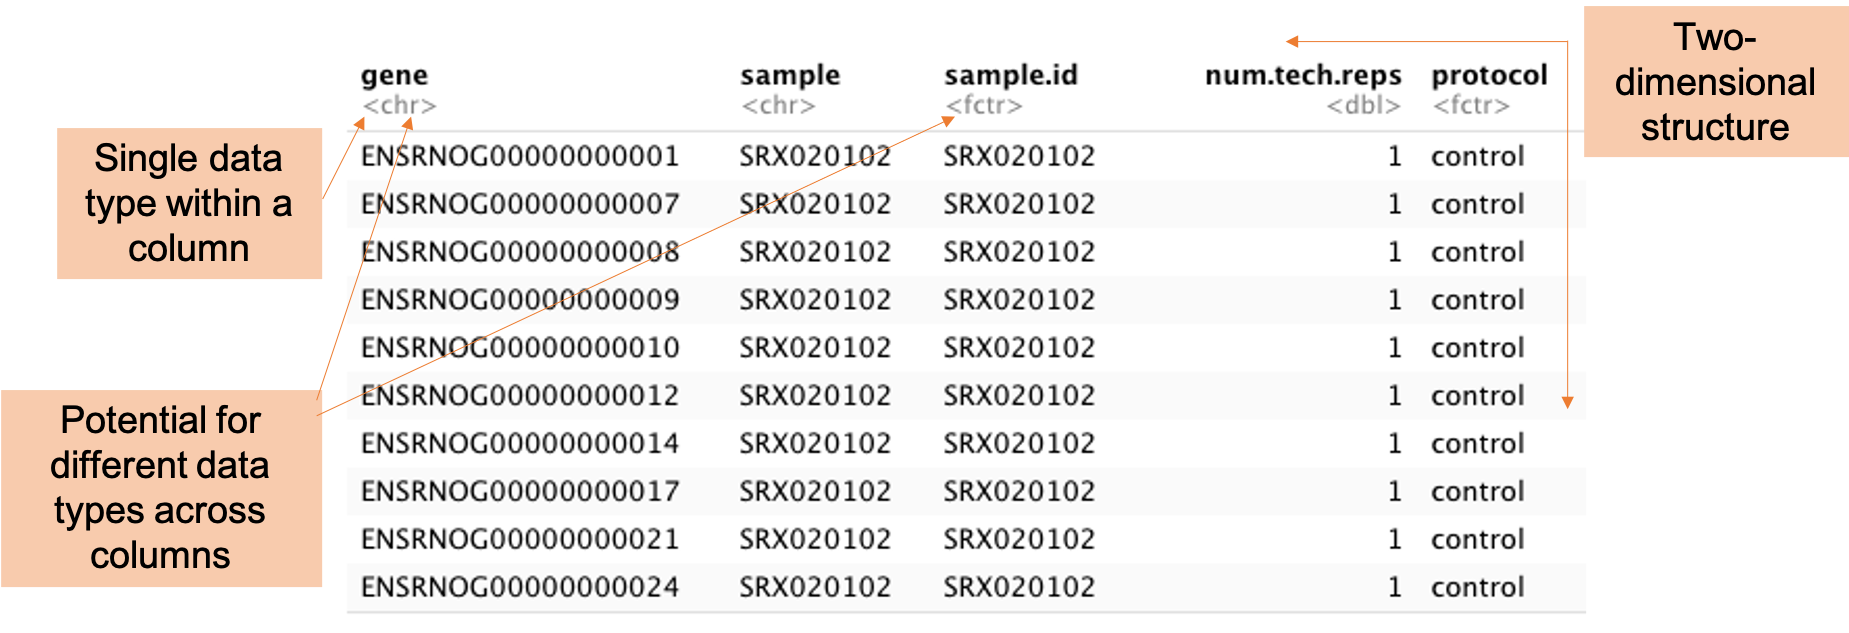
\includegraphics[width=\textwidth]{figures/dataframe} \caption[An example of the dataframe data structure]{An example of the dataframe data structure. This data structure is the most frequently used data structure within the tidyverse approach, and its use is in fact a defining element of the approach.}\label{fig:dfdatastructure}
\end{figure*}

Dataframes like this are very clearly and simply organized. However, they can be
too restrictive in some cases. Sometimes, you might have data that are taken at
different levels of observation---for example, you might have some measurements
that are specific to a specific sample, but then other measurements or data that
are common to the experiment as a whole (metadata).

Also, the simple dataframe structure doesn't have the capacity to store data
taken at these different levels within the same structure (at least, not without
a lot of repetition). Further, the dataframe won't work for massive datasets.
Sometimes, you will get massive amounts of data from equipment like
spectrometers or cytometers, and these datasets can be so big that they can't be
easily read into R. One strategy with massive data is to read in only the bits
you need as you need them, rather than reading in all the data and then
using R commands to work with the full dataset. We'll look later in this module
about how more complex data structures can facilitate this approach when
working with massive data in R.

By addition to dataframes, there are a number of other simple, general purpose
data structures that are often used to store data in R, and that you're likely
to come across as you work in R. These include \textbf{vectors}, which are used to
store one-dimensional strings of data of a single type (e.g., all numeric, or
all character strings; as a note, you can think of each column in a dataframe as
a vector), \textbf{matrices}, which are also used to store data of a single type, but
with a two-dimensional structure, and \textbf{arrays}, which, like matrices and
vectors, store data of a single type, but in three dimensions. Another common
general purpose data structure in R is the \emph{list}, which allows you to combine
data stored in any type of structure to create a single R object, giving
enormous flexibility (but minimal set structure from one object to another).
This data structure is the building block for some of the more complex specific
data structures, which we'll cover next.

\hypertarget{more-complex-data-structures-in-r}{%
\subsection{More complex data structures in R}\label{more-complex-data-structures-in-r}}

The dataframe structure has the advantage of being simple to understand and use.
By using the dataframe as a common structure, the tidyverse approach is able to
create a powerful environment for working with data, because the use of a common
structure allows you to program using small, simple functions that can be
combined in different ways to solve complex tasks.

However, the dataframe lacks flexibility in storing data that does not naturally
follow a two-dimensional structure, and it can struggle to handle massive datasets.
Therefore, in some cases, it is appropriate to adopt approaches that store data
in more complex data structures.

There are two main features of biomedical data---in particular, data collected
from laboratory equipment like flow cytometers and mass spectrometers---that
make it useful to use more complex data structures in R in the earlier stages of
preprocessing the data. First, the data are often very large, in some cases so
large that it is difficult to read them into R. Second, the data might combine
various elements, each with their own natural structures, that you'd like to
keep together as you move through the steps of preprocessing the data.

The data from genomic and other high-throughput experiments
often are too complex and/or large to make dataframes practical as data
structures, at least until data can be simplified through pre-processing.
In this section, we'll look at an approach to pre-processing these data, leveraging
more complex data structures when needed. Once data have been pre-processed,
they are often simplified to the point where they can be stored in a dataframe,
and so it is possible to create workflows that move into a tidyverse approach
once data can reasonably be stored in dataframes. This creates a powerful pipeline,
using more complex tools when necessary and then moving into the more
straightforward tidyverse approach when possible. In the next module, we'll
discuss how you can adopt this type of combined approach.

Most laboratory equipment can output a raw data file that you can then read into R.
For many types of laboratory equipment, these raw data files follow a strict format.
The file formats will often have different pieces of data stored in specific spots.
For example, the equipment might record not only the measurements taken for the
sample, but also information about the setting that were applied to the equipment
while the measurements were taken, the date of the measurements, and other metadata
that may be useful to access when preprocessing the data. Each piece of data may
have different ``dimensions''. For example, the measurements might provide one
measurement per metabolite feature or per marker. Some metadata might also be
provided with these dimensions (e.g., metadata about the markers for flow
cytometry data), but other metadata might be provided a single time per sample
or even per experiment---for example, the settings on the equipment when the
sample or samples were run.

When it comes to data structures, dataframes and other two-dimensional data storage
structures (you can visualize these as similar to the format of data in a spreadsheet,
with rows and columns) work well to store data where all data conform to a common
dimension. For example, a dataframe would work well to store the measurements
for each marker in each sample in a flow cytometry experiment. In this case,
each column could store the values for a specific marker and each row could
provide measurements for a sample. In this way, you could read the measurements
for one marker across all samples by reading down a column, or read the measurements
across all markers for one sample by reading across a row.

When you have data that doesn't conform to these common dimensions {[}unit of
measurement?{]} however, a dataframe may work poorly to store the data. For
example, if you have measurements taken at the level of the equipment settings
for the whole experiment, these don't naturally fit into the dataframe format.
In the ``tidyverse'' approach, one approach to handling data with different units
of measurement is to store data for each unit of measurement in a different
dataframe and to include identifiers that can be used to link data across the
dataframes. More common, however, in R extensions for preprocessing biomedical
data is to use more complex data structures that can store data with different
units of measurement in different slots within the data structure, and use these
in conjunction with specific functions that are built to work with that specific
data structure, and so know where to find each element within the data
structure.

Let's start by looking at how some data might have a structure that is too
complex to fit into a two-dimensional dataframe. Figure
\ref{fig:complexdatastructure} shows an example of different components of data
that may need to be stored in a data structure that is more complex than a
dataframe. Data from a genomic experiment may include data from several levels,
including metadata that describes the entire experiment, as well as assay data,
phenotype data, and gene-level data. More complex data structures in R can be
used to store all these pieces of data inside a single data structure.

\begin{figure}
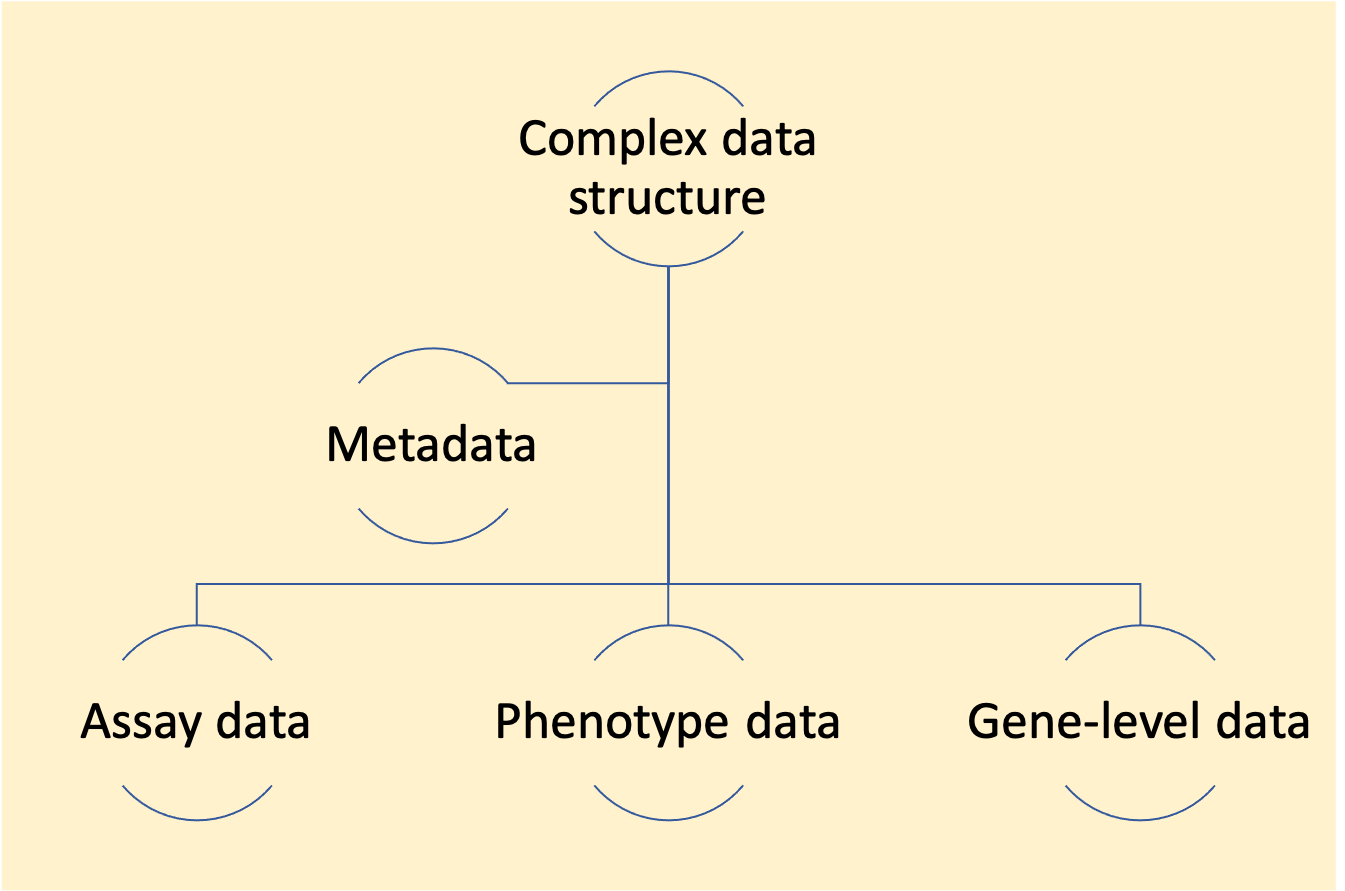
\includegraphics[width=\textwidth]{figures/complex_data_structure} \caption[An example of different components of data that may need to be stored in a data structure that is more complex than a dataframe]{An example of different components of data that may need to be stored in a data structure that is more complex than a dataframe. Data from a genomic experiment may include data from several levels, including metadata that describes the entire experiment, as well as assay data, phenotype data, and gene-level data. More complex data structures in R can be used to store all these pieces of data inside a single data structure.}\label{fig:complexdatastructure}
\end{figure}

The R programming language offers a wide variety of structures that can be
used to store data as you work with it, including steps of preprocessing
and analysis of the data. Some of these structures are defined through the
base R language that you first install, while other structures are specially
defined through the extension R packages you add as you continue to work
with R. These packages are specific to the tasks you aim to do, and if they
define their own data storage structures, those structures are typically
customized to that task.

Many of these more specific data structures are built on the more generic idea
of the \textbf{list} data structure, which provides a very flexible way to combine
other data structures to create a single R object. In R, you can think of a
list data structure as having various slots where it can store data, and
each of these slots can store data stored in another structure. For example,
one slot of a list might store a dataframe of data, while another might store
a vector or a dataframe for a different level of observation. A slot could
even store another list. As an example, if we want to store the type of
data shown in Figure \ref{fig:complexdatastructure}, we could use a list
data structure with one slot that stores the metadata for the experiment,
another that stores a dataframe or matrix with the assay data, another with a
dataframe or matrix that stores the phenotype data, and another with
a dataframe or matrix that stores the gene-level data. Each of these slots in
the list will get a name, and we can use that name to access each of these
pieces of data later. The list, in this case, allows us to store all these
different types of data from an experiment in the same structure in R, so
we can make sure we keep the data together in a single structure, even though
it's too complex to fit in a simple dataframe.

The downside of a general list data structure, however, comes in when it comes
to developing software for data stored in that structure. The general list
structure is very flexible, which is why it can store such different types of
data, but this flexibility means that there's no guarantee about where in
the data structure specific elements might be stored. By comparison, in a
dataframe each row can be assumed to capture an observation, and each column will
capture measurements or characteristics of that observation. Someone can
therefore develop software to work with data stored in that structure, relying
on finding those type of data in those locations in the data structure. When
more complex data are stored in a general list object, the different components
could be store in different ways by different users. For example, for the
type of complex data shown in Figure \ref{fig:complexdatastructure}, one person
might store the metadata in the first slot of a list and the phenotype data
in the second, while another person might store the data in a list with the
metadata in the last slot and the phenotype data in the first.

The way around this problem is to create data structures that build off the
general list structure, but impose some rules that constrain the structure, so
that the same types of data are always stored in the same spot. By doing this,
software developers can develop code to work with data stored in that structure,
with the guarantee that they can always find certain elements of the data in
certain spots in the data structure. Bioconductor makes heavy use of these
types of specialized data structures, typically called ``classes'' in Bioconductor
tutorials and user manuals. This is because, in R, they are created using
one of R's object-oriented approaches, most often one called S4.

Complex data structures like these can be very precise in defining what types of
data they contain and where each component of the data goes. For example,
they may have a ``phenoData'' slot that only will store a specialized
dataframe with phenotype data describing each sample in the experiment {[}?{]},
and another slot named ``featureData'' that will only store a specialized
dataframe with data about each feature (e.g., gene) investigated in the experiment.
With this structure, a software developer can develop a program that inputs
data in this structure, always knowing where to find the feature data or the
phenotype data.

{[}Validation of data as it's entered in an S4 class{]}

\begin{marginfigure}
``Big data is encountered in genomics for two reasons: the size of the
genome and the heterogeneity of populations. Complex organisms, such as
plants and animals, have genomes on the order of billions of base pairs
(the human genome consists of over three billion base pairs). The
diversity of populations, whether of organisms, tissues or cells, means
we need to sample deeply to detect low frequency events. To interrogate
long and/or numerous genomic sequences, many measurements are necessary.
For example, a typical whole genome sequencing experiment will consist
of over one billion reads of 75--100 bp each. The reads are aligned
across billions of positions, most of which have been annotated in some
way. This experiment may be repeated for thousands of samples. Such a
data set does not fit within the memory of a current commodity computer,
and is not processed in a timely and interactive manner. To successfully
wrangle a large data set, we need to intimately understand its structure
and carefully consider the questions posed of it.''

{[}@lawrence2014scalable{]}
\end{marginfigure}

\begin{marginfigure}
``A major challenge in the analysis of scRNA-seq data is the scalability
of analysis methods as datasets increase in size over time. This is
particularly problematic as experiments now frequently produce millions
of cells {[}50--53{]}, possibly across multiple batches, making it
challenging to even load the data into memory and perform downstream
analyses including quality control, batch correction and dimensionality
reduction. Providing analysis methods, such as unsupervised clustering,
that do not require data to be loaded into memory is an imperative step
for scalable analyses. While large-scale scRNA-seq data are now
routinely stored in on-disk data formats (e.g.~HDF5 files), the methods
to process and analyze these data are lagging.''

{[}@hicks2021mbkmeans{]}
\end{marginfigure}

There's a second reason why dataframe structures don't always work for data from
biological experiments, which has to do with the size of data (and so how much
memory it requires). A computer has several ways that it can store data. The
primary storage is closely connected with the computer's processing unit, where
calculations are made, and so data stored in this primary storage can be
processed by code very quickly. R uses this approach, and so when you load data
in R to be stored in one of its traditional data structures, that data is
moved into part of the computer's primary storage (its random access memory, or
RAM).

Data can also be stored in other devices on a computer, including hard drives and
solid state drives that are built into the computer (the computer's secondary
storage devices) or even onto storage devices that can be removed from the
computer, like USB drives or external hard drives (the computer's tertiary storage).
The size of available storage in these devices tends to be much, much larger than
the storage size of the computer's RAM. However, it takes longer to access data
in these secondary storage devices because they aren't directly connected to
the processor, and instead require the data to move into RAM before it can
be accessed by the processor, which is the only part of the computer that can
do things to analyze, modify, or otherwise process the data.

Your data will often be saved on a file in the computer's secondary memory
(e.g., in a file stored on the computer's solid state drive) before you read it
into R, then moved into memory (RAM, part of the primary storage) when you ask
R to load it into a data structure that you can access with code commands in R.
However, the storage size available in RAM will always be much, much smaller than
the storage size in secondary storage devices like solid state drives, and so
with larger data, problems can arise if you try to read data into RAM that is
too large for that primary storage device to accommodate.

The traditional dataframe structure in R is therefore built after
reading the data in memory, into RAM. However, many biological experiments now create
data that is much too large to read into memory for R in a reasonable way
\citep{lawrence2014scalable, hicks2021mbkmeans}. More complex data structures can
allow more sophisticated ways to handle massive data, and so they are often
necessary when working with massive biological datasets, particularly early in
pre-processing, before the data can be summarized in an efficient way. For
example, a more complex data structure could allow much of the data to be left
on disk, and only read into memory {[}RAM?{]} on demand, as specific portions of the
data are needed \citep{gatto2013msnbase, hicks2021mbkmeans}. This approach can be
used to iterate across subsets of the data, only reading parts of the data into
memory at a time \citep{lawrence2014scalable}. Such structures can be designed to
work in a way that, if you are the user, you won't notice the difference in
where the data is kept (on disk versus in memory)---this means you won't have to
worry about these memory management issues, but instead can just gain from
everything going smoothly, even as datasets get very large \citep{gatto2013msnbase}.

{[}Data size, on-disk backends for files, like HDF5 and netCDF---used for flow
cytometry file format?{]}

{[}Potential future direction---developments of tidyverse based front ends for
data stored in databases or on-disk file formats---\texttt{sergeant} package is one
example, also running tidyverse commands on data in database, \texttt{matter} package?,
\texttt{disk.frame} package?{]}

\begin{marginfigure}
``Reading in a large dataset for which you do not have enough RAM is one
easy way to freeze up your computer (or at least your R session). This
is usually an unpleasant experience that usually requires you to kill
the R process, in the best case scenario, or reboot your computer, in
the worst case.''

{[}@peng2016r{]}
\end{marginfigure}

\begin{marginfigure}
``If you use too much memory, R will complain. The key issue is that R
holds all the data in RAM. This is a limitation if you have huge
datasets. The up-side is flexibility---in particular, R imposes no rules
on what data are like.''

{[}@burns2011r{]}
\end{marginfigure}

\begin{marginfigure}
``Random access memory (RAM) is a type of computer memory that can be
accessed randomly: any byte of memory can be accessed without touching
the preceding bytes. RAM is found in computers, phones, tablets and even
printers. The amount of RAM R has access to is incredibly important.
Since R loads objects into RAM, the amount of RAM you have available can
limit the size of data set you can analyse.''

{[}@gillespie2016efficient{]}
\end{marginfigure}

\begin{marginfigure}
``A rough rule of thumb is that your RAM should be three times the size
of your data set.''

{[}@gillespie2016efficient{]}
\end{marginfigure}

\begin{marginfigure}
``RAM is cheap and thinking hurts.''

Uwe Ligges (about memory requirements in R) R-help (June 2007)
\end{marginfigure}

\begin{marginfigure}
``The strengths of R are also its weaknesses: the R API encourages users
to store entire data sets in memory as vectors. These vectors are
implicitly and silently copied to achieve copy-on-write semantics,
contribuing to high memory usage and poor performance.''

{[}@lawrence2014scalable{]}
\end{marginfigure}

\begin{marginfigure}
``Our ultimate goal is to process and summarize a large data set in its
entirety, and iteration enables this by limiting the resource commitment
at a given point in time. Limiting resource consumption generalizes
beyond iteration and is a fundamental technique for computing with big
data. In many cases, it may render iteration unnecessary. Two effective
approaches for being frugal with data are restriction and compression.
Restriction means controlling which data are loaded and lets us avoid
wasting resources on irrelevant or excessive data. Compression helps by
representing the same data with fewer resources.''

{[}@lawrence2014scalable{]}
\end{marginfigure}

\begin{marginfigure}
``The Bioconductor project distributes the software as a number of
different R packages, including Rsamtools, IRanges, GenomicRanges,
GenomicAlignments, Biostrings, rtracklayer, biovizBase and BiocParallel.
The software enables the analyst to conserve computational resources,
iteratively generate summaries and visualize data at arbitrary levels of
detail. These advances have helped to ensure that R and Bioconductor
remain relevant in the age of high-throughput sequencing. We plan to
continue in this direction by designing and implementing abstractions
that enable user code to be agnostic to the mode of data storage,
whether it be memory, files or databases. This will bring much needed
agility to resource allocation and will enable the user to be more
resourceful, without the burden of increased complexity.''

{[}@lawrence2014scalable{]}
\end{marginfigure}

\hypertarget{limitations-to-complex-data-structures}{%
\subsection{Limitations to complex data structures}\label{limitations-to-complex-data-structures}}

In the previous parts of this module, we've highlighted some of the ways that
complex data structures are useful (and even necessary) for parts of the data
pre-processing you may do in R. However, they also have some downsides. In a later
module, we'll talk about how you can use a combined workflow that uses the
Bioconductor approach (with more complex data structures) when necessary, but then
shifts into a tidyverse approach (based on keeping data in a dataframe
structure) as soon as possible in the workflow. Here, we'll describe some of the
limitations of complex data structures to help explain why it's worthwhile to
develop workflows with this combined approach.

The first limitation of using complex data structures is that it requires you to
learn each of the data structures and where they keep different elements of the
data. Each specialized data structure (``class'' in Bioconductor) has defined
rules for each of its data storage slots, and you must become familiar with
these class-specific rules to be able to explore and extract data stored in that
structure.

For example, the \texttt{ExpressionSet} data structure (defined in the \texttt{Biobase}
package in Bioconductor) is used to hold information from high-throughput
assays, like \ldots{} . It includes different slots for data from the assay,
phenotype data (e.g., \ldots), and feature data (e.g., \ldots), as well as slots that
can be used to store things like metadata about the experiment. Each of these
slots has its own name, and you would need to know these names to extract and
explore each of these elements of the data from the structure. If you are doing
an analysis of these type of data, the data might move from this \texttt{ExpressionSet}
data structure into other data structures, for example a \texttt{DGEList} data
structure (defined in the \texttt{edgeR} package in Bioconductor) after you have \ldots,.
and then a \texttt{DGEExact} data structure (also defined in the \texttt{edgeR} package in
Bioconductor) after you have performed {[}differential expression analysis?{]} \ldots{} .
To explore the data after each of these steps, you would need to know the rules,
including the names of each slot, of each of these separate, specialized data
structures.

The second limitation of using complex data structures is that it requires you
to know which functions work with which data structures, and to only use the
appropriate functions with the appropriate data structures. In essence, this
requires you to develop an understanding of how the data moves from one
data structure to another throughout the workflow so that you can apply appropriate
functions at each step.

This also means that you often have to learn a larger set of functions, as
different functions are needed to do similar things to data in different data
structures. For example, if you have a function that can normalize data in one
data structure, it may not work for data stored in a different data structure.
By contrast, when data are stored in a common structure (like a dataframe), the
same functions can always be used, across any step in the pipeline.

There are some approaches that programmers have taken to get around this limitation,
using what are called ``methods''. Methods are functions that run differently
depending on what type of data structure they are given. One example in R is
the \texttt{summary} function, which outputs a summary of the object you input. This
function first checks the class of the object (i.e., the data structure) and
then has different sets of code that it uses depending on what the class is. In
this way, a user can call \texttt{summary} on data stored in many different data
structures and get back something that is appropriate for that data structure.
This helps in limiting the number of function names you, as a user, must remember.
A number of methods exist in R, including \texttt{print}, \texttt{summary}, and \texttt{plot}, that
apply across many different classes of objects (and so across many of the
Bioconductor data structures). However, many of these methods are geared toward
providing ``final'' output---a final summary or plot that you might read and
interpret directly, but not output that serves as a ``step'' in a longer workflow,
so not output that will become input to another function.

\begin{marginfigure}
``There is a cost to the free lunch. That \texttt{print} is generic
means that what you see is not what you get (sometimes). In the printing
of an object you may see a number that you want---an R-squared for
example---but don't know how to grab that number.''

{[}@burns2011r{]}
\end{marginfigure}

Therefore, even the approach of methods can't get around another way that
specialized data structures and their use of specialized functions constrain you
when pre-processing and analyzing data. When data are stored in specialized data
structures, with different structures used for each step of the process, it is
often the case that instead of being able to flexibly combine different
functions in different orders to use small steps to build up to complex
processes, you instead are often constrained to use functions in a predefined
order, as they shift your data from one structure to another. Although the
Bioconductor functions are powerful in pre-processing and analyzing these large,
complex data, they also constrain you somewhat to follow the steps and analysis
imagined by the original package creator, rather than providing flexibility to
create your own series of steps, as the tidyverse approach does.

\begin{center}\rule{0.5\linewidth}{0.5pt}\end{center}

Data in R can be stored in a variety of other formats, too. When you are working
with biological data---in particular, complex or large data output from laboratory
equipment---there can be advantages to using data structures besides dataframes.
In this section, we'll discuss some of the complex characteristics of biomedical
data that recommend the use of data structures in R beyond the dataframe. We'll
also discuss how the use of these other data structures can complicate the use of
``tidyverse'' functions and principles that you might learn in beginning R programming
courses and books. In later modules, we'll discuss how to connect your work in R
to clean and analyze data by performing earlier pre-processing steps using more
complex data structures and then transferring when possible to dataframes for
storing data, to allow you to take advantage of the power and ease of the
``tidyverse'' approach as early as possible in your pipeline.

\hypertarget{complex-versus-simple-structures-for-storing-data}{%
\subsection{Complex versus simple structures for storing data}\label{complex-versus-simple-structures-for-storing-data}}

The R programming language offers a wide variety of structures that can be
used to store data as you work with it, including steps of preprocessing
and analysis of the data. Some of these structures are defined through the
base R language that you first install, while other structures are specially
defined through the extension R packages you add as you continue to work
with R. These packages are specific to the tasks you aim to do, and if they
define their own data storage structures, those structures are typically
customized to that task.

For example, there are packages---including the \texttt{xcms} package, for
example---that allow you to load and preprocess data from LC-MS experiments.
These packages include functionality to load data from a specialized format
output by mass spectometry equipment, as well as identify and align peaks within
the data that might indicate, for example, metabolite features for a
metabolomics analysis. The \texttt{xcms} package defines its own structures that are
used to store data during this preprocessing, and also draws on specialized data
structures defined in other R extension packages, including the \texttt{OnDiskMSnExp}
data object class that is defined by the \texttt{MSnbase} package.

Complex data structures like these can be very precise in defining what types of
data they contain and where each component of the data goes. Later in this and
other modules, we will provide more details about the advantages and
disadvantages of these types of specialized data storage formats, especially in
the context of improving transparency, rigor, and reproducibility across the
steps of preprocessing experimental biomedical data.

By contrast to these more complex data formats, there are a number of simple,
general purpose data structures that are often used to store data in R. These
include \textbf{vectors}, which are used to store one-dimensional strings of data of
a single type (e.g., all numeric, or all character strings), \textbf{matrices}, which
are also used to store data of a single type, but with a two-dimensional
structure, and \textbf{dataframes}, which are used to store multiple vectors of the
same length, and so allow for storing measurements of different data types for
multiple observations.

{[}Figure: examples of these three structures{]}

As you learn R, you will almost certainly learn how to create and work with
these more general data formats, including how to explore the data stored in
each of them. By contrast, you may never learn many of the more complex data
storage formats, especially if you are not using packages from Bioconductor.
However, there are a number of good reasons why R packages---especially those
shared through Bioconductor---define and use more complex data formats. In this
and following modules, we will explain the advantages and disadvantages of
complex versus simpler data storage formats in R. We will also explain how these
advantages and disadvantages weigh out differently in different stages of a data
preprocessing and analysis workflow. Finally, we will describe how you can
leverage both to your advantage, and in particular the tools and approaches that
you can use to shift from a Bioconductor-style approach---with heavy use of
complex data storage formats---early in your preprocessing pipeline to a
tidyverse approach---centered on storing data in a simple, tidy dataframe
object---at later stages, when the data are more suitable to this simpler
storage format, which allows you to leverage the powerful and widely-taught
tidyverse approach in later steps of analysis and visualization.

In these modules, we will focus on explaining these ideas within the R
programming language. This language is a very popular one for both biomedical
data sets and also for more general tasks in data management and analysis.
However, these principles also apply to other programming languages,
particularly those that can be used in an interactive format, including Python
and Julia.

\hypertarget{practice-quiz-3}{%
\subsection{Practice quiz}\label{practice-quiz-3}}

\hypertarget{module16}{%
\section{Complex data types in R and Bioconductor}\label{module16}}

Many R extension packages for pre-processing experimental data use complex
(rather than `tidy') data formats within their code, and many output data in
complex formats. Very recently, the \emph{broom} and \emph{biobroom} R
packages have been developed to extract a `tidy' dataset from a complex data
format. These tools create a clean, simple connection between the complex data
formats often used in pre-processing experimental data and the `tidy' format
required to use the `tidyverse' tools now taught in many introductory R courses.
In this module, we will describe the `list' data structure, the common backbone
for complex data structures in R and provide tips on how to explore and extract
data stored in R in this format, including through the \emph{broom} and
\emph{biobroom} packages.

\textbf{Objectives.} After this module, the trainee will be able to:

\begin{itemize}
\tightlist
\item
  Describe the structure of R's `list' data format
\item
  Take basic steps to explore and extract data stored in R's complex, list-based
  structures
\item
  Describe what the \emph{broom} and \emph{biobroom} R packages can do
\item
  Explain how converting data to a `tidy' format can improve reproducibility
\end{itemize}

\hypertarget{rs-list-data-structure-and-list-based-structures}{%
\subsection{R's list data structure and list-based structures}\label{rs-list-data-structure-and-list-based-structures}}

When you are writing scripts in R to work with your code, if you are at a
point in your pipeline when you can use a ``tidyverse'' approach, then you will
``keep'' your data in a dataframe, as your data structure, throughout your
work. However, at earlier stages in your preprocessing, you may need to use
tools that use other data structures. It's helpful to understand the
basic building blocks of R data structures, so you can find elements of your
data in these other, more customized data structures.

For example, metabolomics data can be collected from the mass spectrometer with
the goal of measuring levels of a large number of metabolite features in each
sample. The data collected from the mass spectrometer will be very large, as
these data describe the full spectra {[}?{]} measured for each sample. Through
pre-processing, these data can be used to align peaks across different samples
and measure the area under each peak {[}?{]} to estimate the level of each
metabolite feature in each sample. This pre-processing will produce a much
smaller table of data, with a structure that can be easily stored in a dataframe
structure (for example, a row for each sample and a column for each metabolite
feature, with the cell values giving the level of each metabolite feature in
each sample). Therefore, before pre-processing, the data will be too complex and
large to reasonably be stored in a dataframe structure, but instead will require
a Bioconductor approach and the use of more complex data structures, while after
pre-processing, the workflow can move into a tidyverse approach, centered on
keeping the data in a dataframe structure.

Many R data structures are built on a general structure called a ``list''. This
data structure is a useful basic general data structure, because it is
extraordinarily flexible. The list data structure is flexible in two
important ways: it allows you to include data of different \emph{types} in the
same data structure, and it allows you to include data with different
dimensions---and data stored hierarchically, including various other data
structures---within the list structure. We'll cover each of these points a bit
more below and describe why they're helpful in making the list a very good
general purpose data structure.

In R, your data can be stored as different \emph{types} of data: whole numbers can be
stored as an \emph{integer} data type, continuous {[}?{]} numbers through a few types of
\emph{floating} data types, character strings as a \emph{character} data type, and logical
data (which can only take the two values of ``TRUE'' and ``FALSE'') as a \emph{logical}
data type. More complex data types can be built using these---for example,
there's a special data type for storing dates that's based on a combination of
an {[}integer?{]} data type, with added information counting the number of days {[}?{]}
from a set starting date (called the {[}Unix epoch?{]}), January 1, 1970. (This
set-up for storing dates allows them to be printed to look like dates, rather
than numbers, but at the same time allows them to be manipulated through
operations like finding out which date comes earliest in a set, determining the
number of days between two dates, and so on.) R uses these different data types
for several reasons. First, by using different data types, R can improve its
efficiency {[}?{]} in storing data. Each piece of data must---as you go deep in the
heart of how the computer works---as a series of binary digits (0s and 1s).
Some types of data can be stored using fewer of these \emph{bits} (\emph{bi}nary dig\emph{its}).
Each measurement of logical data, for example, can be stored in a single bit,
since it only can take one of two values (0 or 1, for FALSE and TRUE, respectively).
For character strings, these can be divided into each character in the string
for storage (for example, ``cat'' can be stored as ``c'', ``a'', ``t''). There is a set
of characters called the ASCII character set that includes the lowercase and
uppercase of the letters and punctuation sets that you see on a standard
US keyboard {[}?{]}, and if the character strings only use these characters, they
can be stored in {[}x{]} bits per character. For numeric data types, integers can
typically be stores in {[}x{]} bits per number, while continuous {[}?{]} numbers,
stored in single or double floating point notation {[}?{]}, are stored in {[}x{]}
and {[}x{]} bits respectively. When R stores data in specific types, it can be
more memory efficient by packing the types of data that can be stored in less
space (like logical data) into very compact structures.

The second advantage of the list structure in R is that it has enormous
flexibility in terms of storing lots of data in lots of possible places. This
data can have different types and even different substructures. Some data
structures in R are very constrained in what type of data they can store and
what structure they use to store it. For example, one of the ``building block''
data structures in R is the vector. This data structure is one dimensional and
can only contain data that have the same data type---you can think of this as a
bead string of values, each of the same type. For example, you could have a
vector that gives a series of names of study sites (each a character string), or
a vector that gives the dates of time points in a study (each a date data type),
or a vector that gives the weights of mice in a study (each a numeric data
type). You cannot, however, have a vector that includes some study site names
and then some dates and then some weights, since these should be in different
data types. Further, you can't arrange the data in any structure except a
straight, one-dimensional series if you are using a vector. The dataframe
structure provides a bit more flexibility---you can expand into two dimensions,
rather than one, and you can have different data types in different columns of
the dataframe (although each column must itself have a single data type).

The list data structure is much more flexible. It essentially allows you to
create different ``slots'', and you can store any type of data in each of these
slots. In each slot you can store any of the other types of data structures in
R---for example, vectors, dataframes, or other lists. You can even store unusual
things like R \emph{environments} {[}?{]} or \emph{pointers} that give the directions to where
data is stored on the computer without reading the data into R (and so saving
room in the RAM memory, which is used when data is ``ready to go'' in R, but which
has much more limited space than the mass {[}?{]} storage on your computer).

Since you can put a list into the slot of a list, it allows you to create deep,
layered structures of data. For example, you could have one slot in a list where
you store the metadata for your experiment, and this slot might itself be a list
where you store one dataframe with some information about the settings of the
laboratory equipement you used to collect the data, and another dataframe that
provides information about the experimental design variables (e.g., which animal
received which treatment). Another slot in the larger list then might have
experimental measurements, and these might either be in a dataframe or, if the
data are very large, might be represented through pointers to where the data is
stored in memory, rather than having the data included directly in the data
structure.

Given all these advantages of the list data structure, then, why not use it all
the time? While it is a very helpful building block, it turns out that its flexibility
can have some disadvantages in some cases. This flexibility means that you can's
always assume that certain bits of data are in a certain spot in each instance
of a list in R. Conversely, if you have data stored in a less flexible structure,
you can often rely on certain parts of the data always being in a certain part of
the data structure. In a ``tidy'' dataframe, for example, you can always assume
that each row represents the measurements for one observation at the unit of
observation for that dataframe, and that each column gives values across all
observations for one particular value that was measured for all the observations.
For example, if you are conducting an experiment with mice, where a certain number
of mice were sacrificed at certain time points, with their weight and the bacteria
load in their lungs measured when the mouse was sacrificed, then you could store
the data in a dataframe, with a row for each mouse, and columns giving the
experimental characteristics for each mouse (e.g., treatment status, time point
when the mouse was sacrificed), the mouse's weight, and the mouse's bacteria
load when sacrificed. You could store all of this information in a list, as
well, but the defined, two-dimensional structure of the dataframe makes it much
more clearly defined where all the data goes in the dataframe structure, while
you could order the data in many ways within a list.

There is a big advantage to having stricter standards for what parts of data go
where when it comes to writing functions that can be used across a lot of data.
You can think of this in terms of how cars are set up versus how kitchens are
set up. Cars are very standardized in the ``interface'' that you get when you sit
down to drive them. The gas and brakes are typically floor pedals, with the gas
to the right of the brake. The steering is almost always provided through a wheel
centered in front of the driver's torso. The mechanism for shifting gears (e.g.,
forward, reverse) is typically to the right of the steering wheel, while
mecahnisms for features like lights and windshield wipers, are typically to the
left of the steering wheel. Because this interface is so standardized, you can
get into a car you've never driven before and typically figure out how to
drive it very quickly. You don't need a lot of time exploring where everything
is or a lot of directions from someone familiar with the car to figure out where
things are. Think of the last time that you drove a rental car---within five minutes,
at most, you were probably able to orient yourself to figure out where everything
you needed was. This is like a dataframe in R---you can pretty quickly figure out
where everything you might need is stored in the data structure, and people can
write functions to use with these dataframes that work well generally across lots
of people's data because they can assume that certain pieces of data are in
certain places.

By contrast, think about walking into someone else's kitchen and orienting yourself
to use that. Kitchen designs do tend to have some general features---most will have
a few common large elements, like a stove somewhere, a refrigerator somewhere,
a pantry somewhere, and storage for pots, pans, and utensils somewhere. However,
there is a lot of flexibility in where each of these are in the kitchen design,
and further flexibility in how things are organized within each of these structures.
If you cook in someone else's kitchen, it is easy to find yourself disoriented in the
middle of cooking a recipe, where a utensil that you can grab almost without
thinking in your own kitchen requires you to stop and search many places in
someone else's kitchen. This is like a list in R---there are so many places that
you can store data in a list, and so much flexibility, that you often find yourself
having to dig around to find a certain element in a list data structure that someone
else has created, and you often can't assume that certain pieces are in certain
places if you are writing your own functions, so it becomes hard to write
functions that are ``general purpose'' for generic list structures in R.

There is a way that list structures can be used in R in a way that retains some
of their flexibility while also leveraging some of the benefits of
standardization. This is R's system for creating \emph{objects}. These object
structures are built on the list data structure, but each object is constrained
to have certain elements of data in certain structures of the data. These
structures cannot be used as easily as dataframes in a ``tidyverse'' approach,
since the tidyverse tools are built based on the assumption that data is stored
in a tidy dataframe. However, they are used in many of the Bioconductor
approaches that allow powerful tools for the earlier stages in preprocessing
biological data. The types of standards that are imposed in the more specialized
objects include which slots the list can have, the names they have, what order
they're in (e.g., in a certain object, the metadata about the experiment might
always be stored in the first slot of the list), and what structures and/or data
types the data in each slot should have.

R programmers get a lot of advantages from using these classes because they can
write functions under the assumption that certain pieces of the data will always
be in the same spot for that type of object. There is still flexibility in the
object, in that it can store lots of different types of data, in a variety of
different structures. While this ``object oriented'' approach in R data structures
does provide great advantages for programmers, and allow them to create powerful
tools for you to use in R, it does make it a little trickier in some cases for
you to explore your data by hand as you work through preprocessing. This is
because there typically are a variety of these object classes that your data
will pass through as you go through different stages of preprocessing, because
different structures are suited to different stages of analysis. Functions often
can only be used for a single class of objects, and so you have to keep track of
which functions pair up with which classes of data. Further, it can be a bit
tricky---at least in comparison to when you have data in a dataframe---to
explore your data by hand, because you have to navigate through different slots
in the object. By contrast, a dataframe always has the same two-dimensional,
rectangular structure, and so it's very easy to navigate and explore data in
this structure, and there are a large number of functions that are built to be
used with dataframes, providing enormous flexibility in what you can do with
data stored in this structure.

While it is a bit trickier to explore your data when it is stored in a
list---either a general list you created, or one that forms the base for a
specialized class structure through functions from a Bioconductor package---you
can certainly learn how to do this navigation. This is a powerful and critical
tool for you to learn as you learn to preprocess your data in R, as you should
\emph{never} feel like you data is stored in a ``black box'' structure, where you can't
peek in and explore it. You should \emph{always} feel like you can take a look at any
part of your data at any step in the process of preprocessing, analyzing, and
visualizing it.

\begin{center}\rule{0.5\linewidth}{0.5pt}\end{center}

\begin{quote}
``There are four primary types of atomic vectors: logical, integer, double,
and character (which contains strings). Collectively, integer and double
vectors are known as numeric vectors.'' \citep{wickham2019advanced}
\end{quote}

\begin{quote}
``\ldots{} the most important family of data types in base R {[}is{]} vectors. \ldots{}
Vectors come in two flavours: atomic vectors and lists. They differ in terms of
their elements' types: for atomic vectors, all elements must have the
same type; for lists, elements can have different types. \ldots{}
Each vector can also have \textbf{attributes}, which you can think of as a
named list of arbitrary metadata. Two attributes are particularly important.
The \textbf{dimension} attribute turns vectors into matrices and arrays and
the \textbf{class} attribute powers the S3 object system.'' \citep{wickham2019advanced}
\end{quote}

\begin{quote}
``A few places in R's documentation call lists generic vectors to emphasise
their difference from atomic vectors.'' \citep{wickham2019advanced}
\end{quote}

\begin{quote}
``Some of the most important S3 vectors {[}are{]} factors, dates and times,
data frames, and tibbles.'' \citep{wickham2019advanced}
\end{quote}

You can use \texttt{typeof} to determine the data type and \texttt{is.{[}x{]}} (\texttt{is.logical},
\texttt{is.character}, \texttt{is.double}, and \texttt{is.integer}) to test if data has a certain
type \citep{wickham2019advanced}.

\begin{quote}
``You may have noticed that the set of atomic vectors does not include a
number of important data structures like matrices, arrays, factors, or
date-times. These types are all built on top of atomic vectors by
adding attributes.'' \citep{wickham2019advanced}
\end{quote}

\begin{quote}
``Adding a \texttt{dim} attribute to a vector allows it to behave like a 2-dimensional
\textbf{matrix} or a multi-dimensional \textbf{array}. Matrices and arrays are primarily
mathematical and statistical tools, not programming tools\ldots{}'' \citep{wickham2019advanced}
\end{quote}

\begin{quote}
``One of the most important vector attributes is \texttt{class}, which underlies the
S3 object system. Having a class attribute turns an object into a \textbf{S3 object},
which means it will behave differently from a regular vector when passed to
a \textbf{generic} function. Every S3 object is built on top of a base type, and often
stores additional information in other attributes.'' \citep{wickham2019advanced}
\end{quote}

\begin{quote}
``Lists are a step up in complexity from atomic vectors: each element can be
any type, not just vectors.'' \citep{wickham2019advanced}
\end{quote}

\begin{quote}
``Lists are sometimes called \textbf{recursive} vectors because a list can contain
other lists. This makes them fundamentally different from atomic vectors.''
\citep{wickham2019advanced}
\end{quote}

\begin{quote}
``The two most important S3 vectors built on top of lists are data frames and
tibbles. If you do data analysis in R, you're going to be using data frames.
A data frame is a named list of vectors with attributes for (column) \texttt{names},
\texttt{row.names}, and its class,''data.frame``\ldots{} In contrast to a regular list, a
data frame has an additional constraint: the length of each of its vectors must
be the same. This gives data frames their rectangular structure\ldots{}'' \citep{wickham2019advanced}
\end{quote}

\begin{quote}
``Data frames are one of the biggest and most important ideas in R, and one of the
things that makes R different from other programming languages. However, in the
over 20 years since their creation, the ways that people use R have changed, and
some of the design decisions that made sense at the time data frames were created
now cause frustration. This frustration led to the creation of the tibble
{[}Muller and Wickham, 2018{]}, a modern reimagining of the data frame. Tibbles are
meant to be (as much as possible) drop-in replacements for data frames that fix
those frustrations. A concise, and fun, way to summarise the main differences is
that tibbles are lazy and surly: they do less and complain more.'' \citep{wickham2019advanced}
\end{quote}

\begin{quote}
``Tibbles are provided by the tibble package and share the same structure as data
frames. The only difference is that the class vector is longer, and includes \texttt{tbl\_df}.
This allows tibbles to behave differentlyin {[}several{]} key ways. \ldots{} tibbles never
coerce their input (this is one feature that makes them lazy)\ldots{} Additionally, while
data frames automatically transform non-syntactic names (unless \texttt{check.names\ =\ FALSE}),
tibbles do not\ldots{} While every element of a data frame (or tibble) must have the
same length, both \texttt{data.frame()} and \texttt{tibble()} will recycle shorter inputs. However,
while data frames automatically recycle columns that are an integer multiple of the
longest column, tibbles will only recycle vectors of length one. \ldots{} There is one
final different: \texttt{tibble()} allows you to refer to variables created during
construction. \ldots{} {[}Unlike data frames,{]} tibbles do not support row names. \ldots{} One
of the most obvious differences between tibbles and data frames is how they
print\ldots{} Tibbles tweak {[}a data frame's subsetting{]} behaviours so that a \texttt{{[}} always
returns a tibble, and a \texttt{\$} doesn't do partial matching and warns if it can't find
a variable (this is what makes tibbles surly). \ldots{} List columns are easier to use
with tibbles because they can be directly included inside \texttt{tibble()} and they
will be printed tidily.'' \citep{wickham2019advanced}
\end{quote}

\begin{quote}
``Since the elements of lists are references to values, the size of a list might
be much smaller than you expect.'' \citep{wickham2019advanced}
\end{quote}

\begin{quote}
``{[}The{]} behavior {[}of environments{]} is different from that of other objects:
environments are always modified in place. This property is sometimes described
as \textbf{reference semantics} because when you modify an environment all existing
bindings to that environment continue to have the same reference. \ldots{} This
basic idea can be used to create functions that `remember' their previous
state\ldots{} This property is also used to implement the R6 object-oriented
programming system\ldots{}'' \citep{wickham2019advanced}
\end{quote}

\hypertarget{exploring-and-extracting-data-from-r-list-data-structures}{%
\subsection{Exploring and extracting data from R list data structures}\label{exploring-and-extracting-data-from-r-list-data-structures}}

To feel comfortable exploring your data at any stage during the preprocessing
steps, you should learn how to investigate and explore data that's stored
in a list structure in R. Because the list structure is the building block
for complex data structures, including Bioconductor class structures, this will
serve you well throughout your work. You should get in the habit of checking
the structure and navigating where each piece of data is stored in the data
structure at each step in preprocessing your data. Also, by checking your data
throughout preprocessing, you might find that there are bits of information
tucked in your data at early stages that you aren't yet using. For example,
many file formats for laboratory equipment include slots for information about
the equipment and its settings during when running the sample. This information
might be read in from the file into R, but you might not know it's there for you
to use if you'd like, to help you in creating reproducible reports that include
this metadata about the experimental equipment and settings.

First, you will want to figure out whether your data is stored in a generic
list, or if it's stored in a specific class-based data structure, which means it
will have a bit more of a standardized structure. To do this, you can run the
\texttt{class} function on your data object. The output of this might be a single value
(e.g., ``list'' {[}?{]}) or a short list. If it's a short list, it will include both
the specific class of the object and, as you go down the list, the more
general data structure types that this class is built on. For example, if the
\texttt{class} function returns this list:

\begin{verbatim}
[Example list of data types---maybe some specific class, then "list"?]
\end{verbatim}

it means that the data's in a class-based structure called \ldots{} which is built on
the more general structure of a list. You can apply to this data any of the functions
that are specifically built for \ldots{} data structures, but you can also apply
functions built for the more general list data structure.

There are several tools you can use to explore data structured as lists in R.
R lists can sometimes be very large---in terms of the amount of data stored in
them---particularly for some types of biomedical data. With some of the tools
covered in this subsection, that will mean that your first look might seem
overwhelming. We'll also cover some tools, therefore, that will let you peel
away levels of the data in a bit more manageable way, which you can use when
you encounter list-structured data that at first feels overwhelming.

First, if your data is stored in a specific class-based data structure, there
likely will also be help files specifically for the class structure that can
help you navigate it and figure out where things are. {[}Example{]}

{[}More about exploring data in list structures.{]}

\begin{center}\rule{0.5\linewidth}{0.5pt}\end{center}

\begin{quote}
``Use \texttt{{[}} to select any number of elements from a vector. \ldots{} \textbf{Positive
integers} return elements at the specified positions. \ldots{} \textbf{Negative
integers} exclude elements at the specified positions\ldots{}
\textbf{Logical vectors} select elements where the corresponding logical vector
is \texttt{TRUE}. This is probably the most useful type of subsetting
because you can write an expression that uses a logical vector\ldots{} If the
vector is named, you can also use \textbf{character vectors} to return elements
with matching names.'' \citep{wickham2019advanced}
\end{quote}

\begin{quote}
``Subsetting a list works in the same way as subsetting an atomic vector.
Using \texttt{{[}} always returns a list; \texttt{{[}{[}} and \texttt{\$} \ldots{} lets you pull out
elements of a list.'' \citep{wickham2019advanced}
\end{quote}

\begin{quote}
``\texttt{{[}{[}} is most important when working with lists because subsetting a list
with \texttt{{[}} always returns a smaller list. \ldots{} Because \texttt{{[}{[}} can return only
a single item, you must use it with either a single positive integer or
a single string.'' \citep{wickham2019advanced}
\end{quote}

\begin{quote}
``\texttt{\$} is a shorthand operator: \texttt{x\$y} is roughly equivalent to \texttt{x{[}{[}"y"{]}{]}}.
It's often used to access variables in a data frame\ldots{} The one important
difference between \texttt{\$} and \texttt{{[}{[}} is that \texttt{\$} does (left-to-right) partial
matching {[}which you likely want to avoid to be safe{]}.'' \citep{wickham2019advanced}
\end{quote}

\begin{quote}
``There are two additional subsetting operators, which are needed for
S4 objects: \texttt{@} (equivalent to \texttt{\$}), and \texttt{slot()} (equivalent to \texttt{{[}{[}}).''
\citep{wickham2019advanced}
\end{quote}

\begin{quote}
``The environment is the data structure that powers scoping. \ldots{} Understanding
environments is not necessary for day-to-day use of R. But they are important to
understand because they power many important features like lexical scoping,
name spaces, and R6 classes, and interact with evaluation to give you powerful
tools for making domain specific languages, like \texttt{dplyr} and \texttt{ggplot2}.''
\citep{wickham2019advanced}
\end{quote}

\begin{quote}
``The job of an environment is to associate, of \textbf{bind}, a set of names to a
set of values. You can think of an environment as a bag of names, with no
implied order (i.e., it doesn't make sense to ask which is the first element
in an environment).'' \citep{wickham2019advanced}
\end{quote}

\begin{quote}
``\ldots{} environments have reference semantics: unlike most R objects, when you
modify them, you modify them in place, and don't create a copy.'' \citep{wickham2019advanced}
\end{quote}

\begin{quote}
``As well as powering scoping, environments are also useful data structures in
their own right because they have reference semantics. There are three common
problems that they can help solve: \textbf{Avoiding copies of large data.} Since
environments have reference semantics, you'll never accidentally create a copy.
But bare environments are painful to work with, so I instead recommend using R6
objects, which are built on top of environments. \ldots{}'' \citep{wickham2019advanced}
\end{quote}

\begin{quote}
``Generally in R, functional programming is much more important than object-oriented
programming, because you typically solve complex problems by decomposing them
into simple functions, not simple objects. Nevertheless, there are important reasons
to learn each of the three {[}object-oriented programming{]} systems {[}S3, R6, and S4{]}:
S3 allows your functions to return rich results with user-friendly display and
programmer-friendly internals. S3 is used throughout base R, so it's important to
master if you want to extend base R functions to work with new types of input.
R6 provides a standardised way to escape R's copy-on-modify semantics. This is
particularly important if you want to model objects that exist independently
of R. Today, a common need for R6 is to model data that comes from a web API,
and where changes come from inside or outside R. S4 is a rigorous system that
forces you to thing carefully about program design. It's particularly well-suited
for building large systems that evolve over time and will receive contributions
from many programmers. This is why it's used by the Bioconductor project, so another
reason to learn S4 is to equip you to contribute to that project.'' \citep{wickham2019advanced}
\end{quote}

\begin{quote}
``The main reason to use OOP is \textbf{polymorphism} (literally: many shapes).
Polymorphism means that a developer can consider a function's interface
separately from its implementation, making it possible to use the same function
form for different types of input. This is closely related to the idea of
\textbf{encapsulation:} the user doesn't need to worry about details of an object
because they are encapsulated behind a standard interface. \ldots{} To be more precise,
\textbf{OO} systems call the type of an object its \textbf{class}, and an implementation for
a specific class is called a \textbf{method}. Roughly speaking, a class defines what an
object \emph{is} and methods describe what that object can \emph{do}. The class defines
the \textbf{fields}, the data possessed by every instance of that class. Classes
are organised in a hierarchy so that if a method does not exist for one
class, its parent's method is used, and the child is said to \textbf{inherit} behaviour.
\ldots{} The process of finding the correct method given a class is called
\textbf{method dispatch}.'' \citep{wickham2019advanced}
\end{quote}

\begin{quote}
``There are two main paradigms of object-oriented programming which differ in how
methods and classes are related. In this book, we'll borrow the terminology of
\emph{Extending R} {[}Chambers 2016{]} and call these paradigms encapsulated and
functional: In \textbf{encapsulated} OOP, methods belong to objects or classes, and
method calls typically look like \texttt{object.method(arg1,\ arg2)}. This is called
encapsulated because the object encapsulates both data (with fields) and
behaviour (with methods), and is the paradigm found in most popular languages.
In \textbf{functional} OOP, methods belong to \textbf{generic} functions, and method calls
look like ordinary function calls: \texttt{generic(object,\ arg2,\ arg3)}. This is called
functional because from the outside it looks like a regular function call, and
internally the components are also functions.'' \citep{wickham2019advanced}
\end{quote}

\begin{quote}
``\textbf{S3} is R's first OOP system\ldots{} S3 is an informal implementation of functional
OOP and relies on common conventions rather than ironclad guarantees.
This makes it easy to get started with, providing a low cost way of solving many
simple problems. \ldots{} \textbf{S4} is a formal and rigorous rewrite of S3\ldots{}
It requires more upfront work than S3, but in return provides more guarantees and greater
encapsulation. S4 is implemented in the base \textbf{methods} package, which is
always installed with R.'' \citep{wickham2019advanced}
\end{quote}

\begin{quote}
``While everything \emph{is} an object, not everything is object-oriented. This confusion
arises because the base objects come from S, and were developed before anyone
thought that S might need an OOP system. The tools and nomenclature evolved
organically over many years without a single guiding principle. Most of the time,
the distinction between objects and object-oriented objects is not important. But
here we need to get into the nitty gritty details so we'll use the terms
\textbf{base objects} and \textbf{OO objects} to distinguish them. \ldots{} Techinally, the difference
between base and OO objects is that OO objects have a `class attribute'.''
\citep{wickham2019advanced}
\end{quote}

\begin{quote}
``An S3 object is a base type with at least a \texttt{class} attribute (other attributes
may be used to store other data). \ldots{} An S3 object behaves differently from its
underlying base type whenever it's passed to a \textbf{generic} (short for generic
function). \ldots{} A generic function defines an interface, which uses a different
implementation depending on the class of an argument (almost always the first
argument). Many base R functions are generic, including the important \texttt{print}\ldots{}
The generic is a middleman: its job is to define the interface (i.e., the arguments)
then find the right implements for the job. The implementation for a specific class
is called a \textbf{method}, and the generic finds the method by performing \textbf{method
dispatch}.'' \citep{wickham2019advanced}
\end{quote}

\begin{quote}
``If you have done object-oriented programming in other languages, you may be
surprised to learn that S3 has no formal definition of a class: to make an object
an instance of a class, you simply set the \textbf{class attribute}. \ldots{} You can determine
the class of an S3 object with \texttt{class(x)}, and see if an object is an instance of
a class using \texttt{inherits(x,\ "classname")}.'' \citep{wickham2019advanced}
\end{quote}

\begin{quote}
``The job of an S3 generic is to perform method dispatch, i.e., find the specific
implementation for a class.'' \citep{wickham2019advanced}
\end{quote}

\begin{quote}
``An important new componenet of S4 is the \textbf{slot}, a named component of the
object that is accessed using the specialised subsetting operator \texttt{@} (pronounced
`at'). The set of slots, and their classes, forms an important part of the
definition of an S4 class.'' \citep{wickham2019advanced}
\end{quote}

\begin{quote}
``Given an S4 object you can see its class with \texttt{is()} and access slots with \texttt{@}
(equivalent to \texttt{\$}) and \texttt{slot()} (equivalent to \texttt{{[}{[}}) \ldots{} Generally, you should only
use \texttt{@} in your methods. If you're working with someone else's class, look for
\textbf{accessor} functions that allow you to safely set and get slot values. \ldots{} Accessors
are typically S4 generics allowing multiple classes to share the same external
interface.'' \citep{wickham2019advanced}
\end{quote}

\begin{quote}
``If you're using an S4 class defined in a package, you can get help on it
with \texttt{class?Person}. To get help for a method, put \texttt{?} in front of a call (e.g.,
\texttt{?age(john)}) and \texttt{?} will use the class of the arguments to figure out which help
file you need.'' \citep{wickham2019advanced}
\end{quote}

\begin{quote}
``Slots {[}in S4 objects{]} should be considered an internal implementation detail:
they can change without warning and user code should avoid accessing them
directly. Instead, all user-accessible slots should be accompanied by a pair
of \textbf{accessors}. If the slot is unique to the class, this can just be a function\ldots{}
Typically, however, you'll define a generic so that multiple classes can used
the same interface'' \citep{wickham2019advancedr}
\end{quote}

\begin{quote}
``The strictness and formality of S4 make it well suited for large teams. Since more
structure is provided by the system itself, there is less need for convention, and new
contributors don't need as much training. S4 tends to require more upfront design
than S3, and this investment is more likely to pay off on larger projects where
greater resources are available. One large team where S4 is used to good effect is
Bioconductor. Bioconductor is similar to CRAN: it's a way of sharing packages
amongst a wider audient. Bioconductor is smaller than CRAN (\textasciitilde1,300 versus \textasciitilde10,000 packages,
July 2017) and the packages tend to be more tightly integrated because of the
shared domain and because Bioconductor has a stricter review process. Bioconductor
packages are not required to use S4, but most will because the key data structures
(e.g., Summarized Experiment, IRanges, DNAStringSet) are built using S4.''
\citep{wickham2019advanced}
\end{quote}

\begin{quote}
``The biggest challenge to using S4 is the combination of increased complexity and
absence of a single source of documentation. S4 is a complex system and it can be
challenging to use effectively in practice. This wouldn't be such a problem if
S4 wasn't scattered through R documentation, books, and websites. S4 needs a
book length treatment, but that book does not (yet) exist. (The documentation for
S3 is no better, but the lack is less painful because S3 is much simpler.)''
\citep{wickham2019advanced}
\end{quote}

\hypertarget{interfacing-between-object-based-and-tidyverse-workflows}{%
\subsection{Interfacing between object-based and tidyverse workflows}\label{interfacing-between-object-based-and-tidyverse-workflows}}

The tidyverse approach in R is based on keeping data in a dataframe structure.
By keeping this common structure, the tidyverse allows for straightforward but
powerful work with your data by chaining together simple, single-purpose
functions. This approach is widely covered in introductory R programming courses
and books. A great starting point is the book \emph{R Programming for Data Science},
which is available both in print and freely online at {[}site{]}. Many excellent
resources exist for learning this approach, and so we won't recover that
information here. Instead, we will focus on how to interface between this
approach and the object-based approach that's more common with Bioconductor
packages. Bioconductor packages often take an object-based approach, and with
good reason because of the complexity and size of many early versions of
biomedical data in the preprocessing process. There are also resources for
learning to use specific Bioconductor packages, as well as some general
resources on Bioconductor, like \emph{R Programming for Bioinformatics} {[}ref{]}.
However, there are fewer resources available online that teach how to coordinate
between these two approaches in a pipeline of code, so that you can leverage the
needed power of Bioconductor approaches early in your pipeline, as you
preprocess large and complex data, and then shift to use a tidyverse approach
once your data is amenible to this more straightforward approach to analysis and
visualization.

The heart of making this shift is learning how to convert data, when possible,
from a more complex, class-type data structure (built on the flexible list
data structure) to the simpler, more standardized two-dimensional dataframe
structure that is required for the tidyverse approach. In this subsection, we'll
cover approaches for converting your data from Bioconductor data structures to
dataframes.

If you are lucky, this might be very straightforward. A pair of packages called
\texttt{broom} and \texttt{biobroom} have been created specifically to facilitate the conversion
of data from more complex structures to dataframes. The \texttt{broom} package was
created first, by David Robinson, to convert the data stored in the objects that
are created by fitting statistical models into tidy dataframes. Many of the functions
in R that run statistical tests or fit statistical models output results in a
more complex, list-based data structure. These structures have nice ``print'' methods,
so if fitting the model or running the test is the very last step of your pipeline,
you can just read the printed output from R. However, often you want to include
these results in further code---for example, creating plots or tables that show
results from several statistical tests or models. The \texttt{broom} package includes
several functions for pulling out different bits of data that are stored in the
complex data structure created by fitting the model or running the test and convert
those pieces of data into a tidy dataframe. This tidy dataframe can then be
easily used in further code using a tidyverse approach.

The \texttt{biobroom} package was created to meet a similar need with data stored in some
of the complex structures commonly used in Bioconductor packages. {[}More about
\texttt{biobroom}.{]}

{[}How to convert data if there isn't a \texttt{biobroom} method.{]} If you are unlucky,
there may not be a \texttt{broom} or \texttt{biobroom} method that you can use for the particular
class-based data structure that your data's in, or it might be in a more general
list, rather than a specific class with a \texttt{biobroom} method. In this case, you'll
need to extract the data ``by hand'' to move it into a dataframe once your data is
simple enough to work with using a tidyverse approach. If you've mastered how to
explore data stored in a list (covered in the last subsection), you'll have a headstart
on how to do this. Once you know where to find each element of the data in the
structure of the list, you can assign these specific pieces to their own R objects
using typical R assignment (e.g., with the \emph{gets arrow}, \texttt{\textless{}-}, or with \texttt{=}, depending
on your preferred R programming style). \ldots{}

\hypertarget{extras}{%
\subsection{Extras}\label{extras}}

{[}Comparison of complexity of biological systems versus complexity of code and
algorithms for data pre-processing---for the later, nothing is unknowable or even
unknown. Someone somewhere is guaranteed to know exactly how it works, what it's
doing, and why. By contrast, with biological systems, there are still things
that noone anywhere completely understands. It's helpful to remember that all
code and algorithms for data pre-processing is knowable, and that the details
are all there if and when you want to dig to figure out what's going on.{]}

{[}There are ways to fully package up and save the computer environment used to
run a pipeline of pre-processing and analysis, including any system settings,
all different software used in analysis steps, and so on. Some of the approaches
that are being explored for this include the use of ``containers'', including
Docker containers. This does allow, typically, for full reproducibility of
the workflow. However, this approach isn't very proactive in emphasizing the
robustness of a workflow or its comprehensibility to others---instead, it
makes the workflow reproducible by putting everything in a black box that must
be carefully unpackaged and explored if someone wants to understand or adapt
the pipeline.{]}

\begin{quote}
``Object-oriented design doesn't have to be over-complicated design, but we've
observed that too often it is. Too many OO designs are spaghetti-like tangles of
is-a and has-a relationships, or feature thick layers of glue in which many of the
objects seem to exist simply to hold places in a steep-sided pyramid of abstractions.
Such designs are the opposite of transparent; they are (notoriously) opaque and
difficult to debug.'' \citep{raymond2003art}
\end{quote}

\begin{quote}
``Unix programmers are the original zealots about modularity, but tend to go about it
in a quiter way {[}that with OOP{]}. Keeping glue layers thin is part of it; more generally,
our tradition teaches us to build lower, hugging the ground with algorithms and structures
that are designed to be simple and transparent.'' \citep{raymond2003art}
\end{quote}

\begin{quote}
``A \emph{standard} is a precise and detailed description of how some artifact is built
or is supposed to work. Examples of software standards include programming
languages (the definition of syntax and semantics), data formats (how information is
represented), algorithmic processing (the steps necessary to do a computation), and
the like. Some standards, like the Word \texttt{.doc} file format, are \emph{de facto} standards---they
have no official standing but everyoen uses them. The word `standard' is best reserved for
formal descriptions, often developed and maintained by a quasi-neutral party like a
government or a consortium, that define how something is built or operated. The definition
is sufficiently complete and precise that separate entities can interact or provide independent
implementations. We benefit from hardware standards all the time, though we may not notice
how many there are. If I buy a new television set, I can plug it inot the electrical outlets
in my home thanks to standards for the size and shape of plugs and the voltage they provide.
The set itself will receive signals and display pictures because of standards for broadcast
and cable television. I can plug other devices into it through standard cables and connectors
like HDMI, USB, S-video and so on. But every TV needs its own remote control and every cell
phone needs a different charger because those have not been standardized. Computing has plenty
of standards as well, including character sets like ASCII and Unicode, programming languages
like C and C++, algorithms for encryption and compression, and protocols for exchanging
information over networks.'' \citep{kernighan2011d}
\end{quote}

\begin{quote}
``Standards are important. They make it possible for independently created things to cooperate,
and they open an area to competition from multiple suppliers, while proprietary systems tend
to lock everyone in. \ldots{} Standards have disadvantages, too---a standard can impede progress if
it is inferior or outdated yet everyone is forced to use it. But these are modest drawbacks
compared to the advantages.'' \citep{kernighan2011d}
\end{quote}

\begin{quote}
``A \emph{class} is a blueprint for constructing a particular package of code and data; each
variable created according to a class's blueprint is known as an \emph{object} of that class.
Code outside of a class that creates and uses an object of that class is known as a \emph{client}
of the class. A \emph{class declaration} names the class and lists all of the \emph{members}, or
items inside that class. Each item is either a \emph{data member}---a variable declared within the
class---or a \emph{method} (also known as a \emph{member function}), which is a function declared within
the class. Member functions can include a special type called a \emph{constructor}, which has the
same name as the class and is invoked implicitly when an object of the class is declared.
In addition to the normal attributes of a variable or function declaration (such as type, and
for functions, the parameter list), each member has an \emph{access specifier}, which indicates
what functions can access the member. A \emph{public member} can be accessed by any code using the
object: code inside the class, a client of the class, or code in a \emph{subclass}, which is a class
that `inherits' all the code and data of an existing class. A \emph{private member} can be
accessed only by the code inside the class. \emph{Protected members} \ldots{} are similar to private
members, except that methods in subclasses can also reference them. Both private and
protected members, though, are inaccessible from client code.'' \citep{spraul2012think}
\end{quote}

\begin{quote}
``An object should be a meaningful, closely knit collection of data and code that operates
on the data.'' \citep{spraul2012think}
\end{quote}

\begin{quote}
``Recognizing a situation in which a class would be useful is essential to reaching the
higher levels of programming style, but it's equally important to recognize situations in
which a class is going to make things worse.'' \citep{spraul2012think}
\end{quote}

\begin{quote}
``The word \emph{encapsulation} is a fancy way of saying that classes put multiple pieces of
data and code together in a single package. If you've ever seen a gelatin medicine capsule
filled with little spheres, that's a good analogy: The patient takes one capsule and swallows
all the individual ingredient spheres inside. \ldots{} From a problem-solving standpoint,
encapsulation allows us to more easily reuse the code from previous problems to solve current
problems. Often, even though we have worked on a problem similar to our current project,
reusing what we learned before still takes a lot of work. A fully encapsulated class can
work like an external USB drive; you just plug it in and it works. FOr this to happen,
though, we must design the class correctly to make sure that the code and data is truly
encapsulated and as independent as possible from anything outside of the class. For example,
a class that references a global variable can't be copied into a new project without
copying the global variable, as well.'' \citep{spraul2012think}
\end{quote}

\begin{quote}
``Beyond reusing classes from one program to the next, classes offer the potential for
a more immediate form of code reuse: inheritance. \ldots{} Using inheritance, we create parent
classes with methods common to two or more child classes, thereby `factoring out' not
just a few lines of code {[}as with helper functions in procedural code{]} but whole methods.''
\citep{spraul2012think}
\end{quote}

\begin{quote}
``One technique we're returned to again and again is dividing a complex problem into
smaller, more manageable pieces. Classes are great at dividing programs up into functional
units. Encapsulation not only holds data and code together in a reusable package; it also
cordons off that data and code from the rest of the program, allowing us to work on that
class, and everything else separately. The more classes we make in a program, the greater
the problem-dividing effect.'' \citep{spraul2012think}
\end{quote}

\begin{quote}
``Some people use the terms \emph{information hiding} and \emph{encapsulation} interchangeable, but
we'll separate the ideas here. As described previously \ldots, encapsulation is
packaging data and code together. Information hiding means separating the interface of a
data structure---the definition of the operations and their parameters---from the implementation
of a data structure, or the code inside the functions. If a class has been written with
information hiding as a goal, then it's possible to change the implementation of the methods
without requiring any changes in the client code (the code that uses the class). Again, we
have to be clear on the term \emph{interface}; this means not only the name of the methods and
their parameter list but also the explanation (perhaps expressed in code documentation) of
what the different methods do. When we talk about changing the implementation without
changing the interface, we mean that we change \emph{how} the class methods work but not
\emph{what} they do. Some programming authors have referred to this as a kind of implicit contract
between the class and the client: The class agrees never to change the effects of
existing operations, and the client agrees to use the class strictly on the basis of its
interface and to ignore any implementation details.'' \citep{spraul2012think}
\end{quote}

\begin{quote}
``So how does information hiding affect problem solving? The principle of information hiding
tells the programmer to put aside the class implementation details when working on the
client code, or more broadly, to be concerned about a particular class's implementation
only when working inside that class. When you can put implementation details out of your
mind, you can eliminate distracting thoughts and concentrate on solving the problem at hand.''
\citep{spraul2012think}
\end{quote}

\begin{quote}
``A final goal of a well-designed class is expressiveness, or what might be broadly called
writability---the ease with which code can be written. A good class, once written, makes
the rest of the code simpler to write in the way that a good function makes code simpler to
write. Classes effectively extend a language, becoming high-level counterparts to basic
low-level features such as loops, if statements, and so forth. \ldots{} With classes, programming
actions that previously took many steps can be done in just a few steps or just one.''
\citep{spraul2012think}
\end{quote}

\begin{quote}
``Right now, in labs across the world, machines are sequencing the genomes of the life
on earth. Even with rapidly decreasing costs and huge technological advancements in
genome sequencing, we're only seeing a glimpse of the biological information contained
in every cell, tissue, organism, and ecosystem. However, the smidgen of total biological
information we're gathering amounts to mountains of data biologists need to work with. At
no other point in human history has our ability to understand life's complexities been so
dependent on our skills to work with and analyze data.'' \citep{buffalo2015bioinformatics}
\end{quote}

\begin{quote}
``Bioinformaticians are concerned with deriving biological understanding from large
amounts of data with specialized skills and tools. Early in biology's history, the
datasets were small and manageable. Most biologists could analyze their own data after
taking a statistics course, using Microsoft Excel on a personal desktop computer.
However, this is all rapidly changing. Large sequencing datasets are widespread, and will
only become more common in the future. Analyzing this data takes different tools, new skills,
and many computers with large amounts of memory, processing power, and disk space.''
\citep{buffalo2015bioinformatics}
\end{quote}

\begin{quote}
``In a relatively short period of time, sequencing costs dropped drastically, allowing
researchers to utilize sequencing data to help answer important biological questions.
Early sequencing was low-throughput and costly. Whole genome sequencing efforts were
expensive (the human genome cost around \$2.7 billion) and only possible through large
collaborative efforts. Since the release of the human genome, sequencing costs have
decreased explonentially until about 2008 \ldots{} With the introduction of next-generation
sequencing technologies, the cost of sequencing a megabase of DNA dropped even more
rapidly. At this crucial point, a technology that was only affordable to large collaborative
sequencing efforts (or individual researchers with very deep pockets) became affordable
to researchers across all of biology. \ldots{} What was the consequence of this drop in
sequencing costs due to these new technologies? As you may have guessed, lots and lots
of data. Biological databases have swelled with data after exponential growth. Whereas once
small databases shared between collaborators were sufficient, now petabytes of useful
data are sitting on servers all over the world. Key insights into biological questions are
stored not just in the unanalyzed experimental data sitting on your hard drive, but also
spinning around a disk in a data center thousands of miles away.'' \citep{buffalo2015bioinformatics}
\end{quote}

\begin{quote}
``To make matters even more complicated, new tools for analyzing biological data are
continually being created, and their underlying algorithms are advancing. A 2012 review
listed over 70 short-read mappers \ldots{} Likewise, our approach to genome assembly has
changed considerably in the past five years, as methods to assemble long sequences
(such as overlap-layout-consensus algorithms) were abandoned with the emergence of
short high-throughput sequencing reads. Now, advances in sequencing chemistry are
leading to longer sequencing read lengths and new algorithms are replacing others that
were just a few years old. Unfortunately, this abundance and rapid development of
bioinformatics tools has serious downsides. Often, bioinformatics tools are not adequately
benchmarked, or if they are, they are only benchmarked in one organism. This makes it
difficult for new biologists to find and choose the best tool to analyze their data.
To make matters more difficult, some bioinformatics programs are not actively developed
so that they lose relevance or carry bugs that could negatively affect results. All of
this makes choosing an appropriate bioinformatics program in your own research difficult.
More importantly, it's imperative to critically assess the output of bioinformatics
programs run on your own data.'' \citep{buffalo2015bioinformatics}
\end{quote}

\begin{quote}
``With the nature of biological data changing so rapidly, how are you supposed to
learn bioinformatics? With all of the tools out there and more continually being
created, how is a biologist supposed to know whether a program will work appropriately
on her organism's data? The solution is to approach bioinformatics as a bioinformatician
does: try stuff, and assess the results. In this way, bioinformatics is just about having
the skills to experiment with data using a computer and understanding your results.
The experimental part is easy: this comes naturally to most scientists. The limiting
factor for most biologists is having the data skills to freely experiment and work with
large data on a computer.'' \citep{buffalo2015bioinformatics}
\end{quote}

\begin{quote}
``Unfortunately, many of the biologist's common computational tools can't scale to the
size and complexity of modern biological data. Complex data formats, interfacing
numerous programs, and assessing software and data make large bioinformatics datasets
difficult to work with.'' \citep{buffalo2015bioinformatics}
\end{quote}

\begin{quote}
``In 10 years, bioinformaticians may only be using a few of the bioinformatics
software programs around today. But we most certainly will be using data skills and
experimentation to assess data and methods of the future.'' \citep{buffalo2015bioinformatics}
\end{quote}

\begin{quote}
``Biology's increasing use of large sequencing datasets is changing more that the tools
and skills we need: it's also changing how reproducible and robust our scientific
findings are. As we utilize new tools and skills to analyze genomics data, it's
necessary to ensure that our approaches are still as reproducible and robust as
any other experimental approaches. Unfortunately, the size of our data and the complexity
of our analysis workflows make these goals especially difficult in genomics.''
\citep{buffalo2015bioinformatics}
\end{quote}

\begin{quote}
``The requisite of reproducibility is that we share our data and methods. In the pre-genomics
era, this was much easier. Papers coule include detailed method summaries and entire
datasets---exactly as Kreitman's 1986 paper did with a 4,713bp Adh gene flanking sequence
(it was embedded in the middle of the paper). Now papers have long supplementary methods,
code, and data. Sharing data is no longer trivial either, as sequencing projects can include
terabytes of accompanying data. Reference genomes and annotation datasets used in analyses are
constantly updated, which can make reproducibility tricky. Links to supplemental materials,
methods, and data on journal websites break, materials on faculty websites disappear when
faculty members move or update their sites, and software projects become stale when
developers leave and don't update code. \ldots{} Additionally, the complexity of bioinformatics
analyses can lead to findings being susceptible to errors and technical confounding.
Even fairly routine genomics projects can use dozens of different programs, complicated
input paramter combinations, and many sample and annotation datasets; in addition, work
may be spread across servers and workstations. All of these computational data-processing
steps create results used in higher-level analyses where we draw our biological conclusions.
The end result is that research findings may rest on a rickety scaffold of numerous
processing steps. To make matters worse, bioinformatics workflows and analyses are usually
only run once to produce results for a publication, and then never run or tested again.
These analyses may rely on very specific versions of all software used, which can make it
difficult to reproduce on a different system. In learning bioinformatics data skills, it's
necessary to concurrently learn reproducibility and robust best practices.''
\citep{buffalo2015bioinformatics}
\end{quote}

\begin{quote}
``When we are writing code in a programming language, we work most of the time with RAM,
combining and restructuring data values to produce new values in RAM. \ldots{} The computer memory
in RAM is a series of 0's and 1's, just like the computer memory used to store files in mass
storage. In order to work with data values, we need to get those values into RAM in some
format. At the basic level of representing a single number or a single piece of text, the
solution is the same as it was in Chapter 5 {[}on file formats for mass storage{]}. Everything
is represented as a pattern of bits, using various numbers of bytes for different sorts of
values. In R, in an English locale, and on a 32-bit operating system, a single character
usually takes up one byte, an integer takes up four bytes, and a real number 8 bytes.
Data values are stored in different ways depending on the \textbf{data type}---whether the values
are numbers or texts.'' \citep{murrell2009introduction}
\end{quote}

\begin{quote}
``ALthough we do not often encounter the details of the memory representation, except
when we need a rough estimate of how much RAM a data set might require, it is
important to keep in mind what sort of data type we are working with because the computer
code that we will produce different results for different data types. For example,
we can only calculate an average if we are dealing with values that have been stored
as text.'' \citep{murrell2009introduction}
\end{quote}

\begin{quote}
``Another important issue is how \emph{collections} of values are stored in memory. The
tasks that we will consider will typically involve working with an entire data set,
or an entire variable from a data set, rather than just a single value, so we need
to have a way to represent several related values in memory. This is similar to the
problem of deciding on a storage format for a data set\ldots{} However, rather than talking
about different file formats, {[}in this case{]} we will talk about different \textbf{data
structures} for storing a collection of data values in RAM. \ldots{} It will be important
to always keep close in our minds what data type we are working with and what sort
of data structure we are working with.'' \citep{murrell2009introduction}
\end{quote}

\begin{quote}
``Every individual data value has a data type that tells us what sort of value it
is. The most common data types are numbers, which R calls \textbf{numeric values}, and
text, which R calls \textbf{character values}.'' \citep{murrell2009introduction}
\end{quote}

\begin{quote}
``\textbf{Vectors:} A collection of values that all have the same data type. The
\textbf{elements} of a vector are all numbers, giving a \textbf{number vector}, or all
character values, giving a \textbf{character vector.}'' \citep{murrell2009introduction}
\end{quote}

\begin{quote}
``\textbf{Data frames:} A collection of vectors that all have the same length. This is
like a matrix, except that each column can contain a different data type.''
\citep{murrell2009introduction}
\end{quote}

\begin{quote}
``\textbf{Lists:} A collection of data structures. The \textbf{components} of a list can
be simply vectors---similar to a data frame, but with each column allowed to have
a different length. However, a list can also be a much more complicated
structure. This is a very flexible data structure. Lists can be used to store
any combination of data values together.'' \citep{murrell2009introduction}
\end{quote}

\begin{quote}
``Notice the way that lists are displayed. The first component of the list
starts with the component indes, \texttt{{[}{[}1{]}{]}}, followed by the contents of this
component\ldots The second component of the list starts with the component
index \texttt{{[}{[}2}{]}{]} followed by the contenets of this component\ldots{}'' \citep{murrell2009introduction}
\end{quote}

\begin{quote}
``A list is a very flexible data structure. It can have any number of \textbf{components},
each of which can be any data structure of any length or size. A simple
example is a data-frame-like structure where each column can have a different
length, but much more complex structures are also possible. For example, it is
possible for a component of a list to be another list.'' \citep{murrell2009introduction}
\end{quote}

\begin{quote}
``Anyone who has worked with a computer should be familiar with the idea of
a list containing another list because a directory or folder of files has this sort
of structure: a folder contains multiple files of different kinds and sizes and
a folder can contain other folders, which can contain more files or even more
folders, and so on. Lists allow for this kind of hierarchical structure.''
\citep{murrell2009introduction}
\end{quote}

\begin{quote}
``One of the most basic ways that we can manipulate data structures is to
\textbf{subset} them---select a smaller portion from a larger data structure. This
is analogous to performing a query on a database. \ldots{} R has very powerful
mechanisms for subsetting\ldots{} A subset from a vector may be obtained by
appending an \textbf{index} within square brackets to the end of a symbol name. \ldots{}
The index can be a vector of any length \ldots{} The index does not have to be
a contiguous sequence, and it can include repetitions\ldots{} As well as using
integers for indices, we can use logical values\ldots{} A data frame can also
be indexed using square brackets, though slightly differently because we have
to specify both which rows \emph{and} which columns we want \ldots{} When a data structure
has named components, a subset may be selected using those names.''
\citep{murrell2009introduction}
\end{quote}

\begin{quote}
``Single square bracket subsetting on a data frame is like taking an egg container
that contains a dozen eggs and chopping up the \emph{container} so that we are left
with a smaller egg container that contains just a few eggs. Double square bracket
subsetting on a data frame is like selecting just one \emph{egg} from an egg container.''
\citep{murrell2009introduction}
\end{quote}

\begin{quote}
``We can often get some idea of what sort of data structure we are working with
by simply viewing how the data are displayed on screen. However, a more definitive
answer can be obtained by calling the \texttt{class()} function. \ldots{} Many R functions
return a data structure that is not one of the basic data structures that we have
already seen {[}like the `xtabs' and `table' classes{]}. \ldots{} We have not seen either
of these data structures before. However, much of what we know about working with
the standard data structures \ldots{} will work with any new class that we encounter.
For example, it is usually possible to subset any class using the standard
square bracket syntax. \ldots{} Where appropriate, arithmetic and comparisons will
also generally work\ldots{} Furthermore, if necessary, we can ofter resort to coercing
a class to something more standard and familiar.'' \citep{murrell2009introduction}
\end{quote}

\begin{quote}
``Dates are an important example of a special data structure. Representing
dates as just text is convenient for humans to view, but other representations
are better for computers to work with. \ldots{} Having a special class for dates
means that we can perform tasks with dates, such as arithmetic and comparisons,
in a meaningful way, something we could not do if we stored the date as just
a character value.'' \citep{murrell2009introduction}
\end{quote}

\begin{quote}
``The Date class stores date values as integer values, representing the number
of days since January 1st 1970, and automatically converts the numbers to
a readable text value to display the dates on the screen.'' \citep{murrell2009introduction}
\end{quote}

\begin{quote}
``When working with anything but tiny data sets, basic reatures of the data
set cannot be determined by just viewing the data values. {[}There are{]} a number of
functions that are useful for obtaining useful summary features from a data structure.
The \texttt{summary()} function produces summary information for a data structure\ldots{} The
\texttt{length()} function is useful for determining the number of values in a vector or
the number of components in a list. \ldots{} The \texttt{str()} function (short for `structure')
is useful when dealing with large objects because it only shows a sample of the values
in each part of the object, although the display is very low-level so it may not always
make things clearer. \ldots{} Another function that is useful for inspecting a large
object is the \texttt{head()} function. This shows just the first few elemeents of an
object, so we can see the basic structure without seeing all of the values.''
\citep{murrell2009introduction}
\end{quote}

\begin{quote}
``Generic functions \ldots{} will accept many different data structures as
arguments. \ldots{} a generic function adapts itself to the data structure it is
given. Generic functions do different things when given different data structures.''
\citep{murrell2009introduction}
\end{quote}

\begin{quote}
``An example of a generic function is the \texttt{summary()} function. The result of a
call to \texttt{summary()} sill depend on what sort of data structure we provide.''
\citep{murrell2009introduction}
\end{quote}

\begin{quote}
``Generic functions are another reason why it is easy to work with data in R; a
single function will produce a sensible result no matter what data structure
we provide. However, generic functions are also another reason why it is so
important to be aware of what data structures we are working with. Without
knowing what sort of data we are using, we cannot know what sort of result to
expect from a generic function.'' \citep{murrell2009introduction}
\end{quote}

\begin{quote}
``R has become very popular and is now being used for projects that require
substantial software engineering as well as its continued widespread use as
an interactive environment for data analysis. This essentially means that
there are two masters---\emph{reliability} and \emph{ease of use}. S3 is indeed easy to
use, but can be made unreliable through nothing other than bad luck, or
a poor choice of names, and hence is not a suitable paradigm for constructing
large systems. S4, on the other hand, is better suited for developing large
software projects but has an increased complexity of use.'' \citep{gentleman2008r}
\end{quote}

\begin{quote}
``Object-oriented programming has become a widely used and valuable tool for
software engineering. Much of its value derives from the fact that it is often
easier to design, write, and maintain software when there is some clear
separation of the data representation from the operations that are to be
performed on it. In an OOP system, real physical things \ldots{} are generally
represented by classes, and methods (functions) are written to handle the
different manipulations that need to be performed on the objects.'' \citep{gentleman2008r}
\end{quote}

\begin{quote}
``The views that many people have of OOP have been based largely on
exposure to languages like Java, where the system can be described as class-centric.
In a a class-centric system, classes define objects and are repositories for
the methods that act on those objects. In contrast, languages such as \ldots{} R
separate the class specification from the specification of generic functions,
and could be described as function-centric systems.'' \citep{gentleman2008r}
\end{quote}

\begin{quote}
``The genome of every organism is encoded in chromosomes that consist of either
DNA or RNA. High throughput sequencing technology has made it possible to determine
the sequence of the genome for virtually any organism, and there are many that are
currently available. \ldots{} However, in many cases, either the exact nucleotide at
any location is unknown, or is variable, and the International Union of Pure and
Applied Chemistry (IUPAC) has provided a standard nomenclature suitable for
representing such sequences. The alphabet for dealing with protein sequences
is based on the 20 amino acids. \ldots{} The basic class used to hold strings {[}in the
\textbf{Biostrings} package{]} is the \emph{BString} class, which has been designed to be
efficient in its handling of large character strings. Subclasses include
\emph{DNAString}, \emph{RNAString}, and \emph{AAString} (for holding amino acid sequences).
The \emph{BStringViews} class holds a set of \emph{views} on a single \emph{BString} instance;
each view is essentially a substring of the underlying \emph{BString} instance. Alignments
are stored using the \emph{BStringAlign} class.'' \citep{gentleman2008r} {[}More on functions that
work with these classes on p.~171{]}
\end{quote}

\begin{quote}
``A number of complete genomes, represented as \emph{DNAString} objects, are provided
through the Bioconductor project. They rely on the infrastructure in the \textbf{BSgenome}
package, and all such packages have names that begin with \texttt{BSgenome}. You can find the
list of available genomes using the \texttt{available.genomes} function.'' \citep{gentleman2008r}
\end{quote}

\begin{quote}
``Atomic vectors are the most basic of all data structures. An atomic vector
contains some number of values of the same type; that number could be zero.
Atomic vectors can contain integers, doubles, logicals or character strings.
Both complex numbers and raw (pure bytes) have atomic representations \ldots{}
Character vectors in the S language are vectors of character strings, not the
vectors of characters. For example, the string `super' would be represented as
a character vector of length one, not of lenth five\ldots{}'' \citep{gentleman2008r}
\end{quote}

\begin{quote}
``Lists can be used to store items that are not all of the same type. \ldots{}
Lists are also referred to as generic vectors since they share many of the properties
of vectors, but the elements are allowed to have different types.'' \citep{gentleman2008r}
\end{quote}

\begin{quote}
``Lists can be of any length, and the elements of a list can be named, or not.
Any R object can be an element of a list, including another list\ldots{}'' \citep{gentleman2008r}
\end{quote}

\begin{quote}
``A \texttt{data.frame} is a special kind of list. Data frames were created to provide a
common structure for storing rectangular data sets and for passing them to
different functions for modeling and visualization. In many cases a data set can be
thought of as a rectangular structure with rows corresponding to cases and columns
corresponding to the different variables that were measured on each of the cases. One
might think that a matrix would be the appropriate representation, but that is only
true if all of the variables are of the same type, and this is seldom the case.''
\citep{gentleman2008r}
\end{quote}

\begin{quote}
``{[}Data frames{]} are essentially a list of vectors, with one vector for each variable.
It is an error if the vectors are not all of the same length.'' \citep{gentleman2008r}
\end{quote}

\begin{quote}
``Sometimes it will be helpful to find out about an object. Obvious functions to
try are \texttt{class} and \texttt{typeof}. But many find that both \texttt{str} and \texttt{object.size} are
more useful. \ldots{} The functions \texttt{head} and \texttt{tail} are convenience functions that list
the first few, or the last few, rows of a matrix.'' \citep{gentleman2008r}
\end{quote}

\begin{quote}
``The S langauge has its roots in the Algol family of languages and has adopted some
of the general vector subsetting and subscripting techniques that were available in
languages such as APL. This is perhaps one area wehre programmers more familiar with
other languages fail to make appropriate use of the available functionality. \ldots{}
There are slight differents between subsetting of vectors, arrays, lists, data.frames,
and enviroments that can sometimes catch the unwary. But there are also many
commonalities. \ldots{} Subsetting can be carried out by three different operators:
the single square bracket \texttt{{[}}, the double square bracket \texttt{{[}{[}}, and the dollar, \texttt{\$}.
We note that each of these three operators are actually generic functions and users
can write methods that extend and override them\ldots{} One way of describing the behavior
of the single bracket operator is that the type of the return value matches the type
of the value it is applied to. Thus, a single bracket subset of a list is a list
itself. \ldots{} Both \texttt{{[}{[}} and \texttt{\$} extract a single value. There are some differences
between the two; \texttt{\$} does not evaluate its second argument while \texttt{{[}{[}} does, and hence
one can use expressions. The \texttt{\$} operator uses partial matching when extracting
named elements but \texttt{{[}} and \texttt{{[}{[}} do not.'' \citep{gentleman2008r}
\end{quote}

\begin{quote}
``Subsetting plays two roles in the S language. One is an extraction role, where a subset
of a vector is identified by a set of supplied indices and the resulting subset is
returned as a value. Venables and Ripley (2000) refer to this as \emph{indexing}. The
second purpose is subset assignment, where the goal is to identify a subset of
values that should have their values changed; we call this subset assignment.''
\citep{gentleman2008r}
\end{quote}

\begin{quote}
``There are four basic types of subscript indices: positive integers, negative
integers, logical vectors, and character vectors. These four types cannot be mixed\ldots{}
For matrix and array subscripting, one can use different types of subscripts for
the different dimensions. Not all vectors, or recursive objects, support all types
of subscripting indices. For example, atomic vectors cannot be subscripted using
\texttt{\$}, while environments cannot be subscripted using \texttt{{[}}.'' \citep{gentleman2008r}
\end{quote}

\begin{quote}
``In bioinformatics, the plain-text data we work with is often encoded in \emph{ASCII}.
ASCII is a character encoding scheme that uses 7 bits to represent 128 different
values, including letters (upper- and lowercase), numbers, and special nonvisible
characters. While ASCII only uses 8 bits, nowadays computers use an 8-bit \emph{byte}
(a unit representing 8 bits) to store ASCII characters. More information about
ASCII is available in your terminal through \texttt{man\ ascii}.'' \citep{buffalo2015bioinformatics}
\end{quote}

\begin{quote}
``Some files will have non-ASCII encoding schemes, and may contain special characters.
The most common character encoding scheme is UTF-8, which is a superset of ASCII
but allows for special characters.'' \citep{buffalo2015bioinformatics}
\end{quote}

\begin{quote}
``Bioinformatics data is often text---for example, the As, Cs, Ts, and Gs in
sequencing read files or reference genomes, or tab-delimited files fo gene coordinates.
The text data in bioinformatics is often large, too (gigabytes or more that can't
fit into your computer's memory at once). This is why Unix's philosophy of
handling text streams is useful to bioinformatics: text streams allow us to
do processing on a \emph{stream} of data rather than holding it all in memory.''
\citep{buffalo2015bioinformatics}
\end{quote}

\begin{quote}
``Exploratory data analysis plays an integral role throughout an entire bioinformatics
project. Exploratory data analysis skills are just as applicable in analyzing intermediate
bioinformatics data (e.g., are fewer reads from this sequencing lane aligning?) as
they are in making sense of results from statistical analyses (e.g., what's the distribution
of these p-values, and do they correlate with possible confounders like gene length?).
These exploratory analyses need not be complex or exceedingly detailed (many patterns
are visible with simple analyses and visualization); it's just about wanting to look
into the data and having the skill set to do so.'' \citep{buffalo2015bioinformatics}
\end{quote}

\begin{quote}
``Functions like \texttt{table()} are generic---they are designed to work with objects of
all kinds of classes. Generic functions are also designed to do the right thing
depending on the class of the object they're called on (in programming lingo, we
say that the function is \emph{polymorphic}).'' \citep{buffalo2015bioinformatics}
\end{quote}

\begin{quote}
``It's quite common to encounter genomics datasets that are difficult to load into
R because they're large files. This is either because it takes too long to load the
entire dataset into R, or your machine simply doesn't have enough memory. In many
cases, the best strategy is to reduce the size of your data somehow: summarizing data
in earlier processing steps, omitting unnecessary columns, splitting your data into
chunks (e.g., working with a chromosome at a tiem), or working on a random subset
of your data. Many bioinformatics analyses do not require working on an entire
genomic dataset at once, so these strategies can work quite well. These approaches
are also the only way to work with data that is truly too large to fit in your
machine's memory (apart from getting a machine with more memory).'' \citep{buffalo2015bioinformatics}
\end{quote}

\begin{quote}
``If your data is larger than the available memory on your machine, you'll need to
use a strategy that keeps the bulk of your data out of memory, but still allows for
each access from R. A good solution for moerately large data is to use SQLite and
query out subsets for computation using the R package \texttt{RSQLite}. \ldots{} Finally \ldots{}
many Unix data tools have versions that work on gzipped files: \texttt{zless}, \texttt{zcat} (\texttt{gzcat}
on BSD-derived systems like Mac OS X), and others. Likewise, R's data-reading
functions can also read gzipped files directly---there's some slight performance
gains in reading in gzipped files, as there are fewer bytes to read off of
(slow) hard disks.'' \citep{buffalo2015bioinformatics}
\end{quote}

\begin{quote}
``Quite often, data we load in to R will be in the wrong \emph{shape} for what we want to
do with it. Tabular data can come in two different formats: \emph{long} and \emph{wide}. \ldots{}
In many cases, data is recorded by humans in wide format, but we need data in long
format when working with and plotting statistical modeling functions.''
\citep{buffalo2015bioinformatics}
\end{quote}

\begin{quote}
``Exploratory data analysis emphasizes visualization as the best tool to understand
and explore our data---both to learn what the data says and what its limitations are.''
\citep{buffalo2015bioinformatics}
\end{quote}

\begin{quote}
``R vectors require all elements to have the same data type (that is, vectors are
\emph{homogeneous}). They only support the six data types discussed earlier (integer, double,
character, logical, complex, and raw). In contrast, R's lists are more versatile: Lists can
contain elements of different types (they are \emph{heterogenesou}); Elements can be \emph{any}
object in R (vectors with different types, other lists, environments, dataframes,
matrices, functions, etc.); Because lists can store other lists, they allow for storing
data in a recursive way (in contrast, vectors cannot contain other vectors.''
\citep{buffalo2015bioinformatics}
\end{quote}

\begin{quote}
``The versatility of lists make them indispensable in programming and data analysis with
R.'' \citep{buffalo2015bioinformatics}
\end{quote}

\begin{quote}
``As with R's vectors, we can extract subsets of a list or change values of
specific elements using indexing. However, accessing elements from an R list is
slightly different than with vectors. Because R's list can contain objects with
different types, a subset containing multiple list elements could contain objects with
different types. Consequently, the only way to return a subset of more than one
list element is with another list. As a result, there are two indexing operators for lists:
one for accessing a subset of multiple elements as a list (the single bracket\ldots) and
one for accessing an element within a list (the double bracket\ldots).''
\citep{buffalo2015bioinformatics}
\end{quote}

\begin{quote}
``Because R's lists can be nested and contain any type of data, list-based data
structures can grow to be quite complex. In some cases, it can be difficult to
understand the overall structure of some lists. The function \texttt{str()} is a convenient
R function for inspecting complex data structures. \texttt{str()} prints a line for each
contained data structure, complete with its type, length (or dimensions), and the
first few elements it contains. \ldots{} For deeply nested lists, you can simplify \texttt{str()\textquotesingle{}\textquotesingle{}s\ output\ by\ specifying\ the\ maximum\ depth\ of\ nested\ structure\ to\ return\ with}str()\texttt{\textquotesingle{}s\ \ second\ argument,}max.level\texttt{.\ By\ default,}max.level\texttt{is}NA`, which returns all
nested structures.'' \citep{buffalo2015bioinformatics}
\end{quote}

\begin{quote}
``Understanding R's data structures and how subsetting works are fundamental to
having the freedom in R to explore data any way you like.'' \citep{buffalo2015bioinformatics}
\end{quote}

\begin{quote}
``Some of Bioconductor's core packages: \textbf{GenomicRanges:} Used to represent and
work with genomic ranges; \textbf{GenomicFeatures:} used to represent and work with ranges
that represent gene models and other features of a genome (genes, exons, UTRs,
transcripts, etc.); \textbf{Biostrings} and \textbf{BSgenome:} Used for manipulating genome
sequence data in R\ldots{} \textbf{rtracklayer:} Used for reading in common bioinformatics formats
like BED, GTF/GFF, and WIG.'' \citep{buffalo2015bioinformatics}
\end{quote}

\begin{quote}
``The \texttt{GenomicRanges} package introduces a new class called \texttt{GRanges} for storing
genomic ranges. The \texttt{GRanges} builds off of \texttt{IRanges}. \texttt{IRanges} objects are used
to store ranges of genomic regions on a single sequence, and \texttt{GRanges} objects contain
the two other pieces of information necessary to specify a genomic location:
sequence name (e.g., which chromosome) and strand. \texttt{GRanges} objects also have
\emph{metadata columns}, which are the data linked to each genomic range.''
\citep{buffalo2015bioinformatics}
\end{quote}

\begin{quote}
``All metadata attached to a \texttt{GRanges} object are stored in a \texttt{DataFrame}, which
behaves identically to R's base \texttt{data.frame} but supports a wider variety of
column types. For example, \texttt{DataFrames} allow for run-length encoded vectors
to save memory \ldots{} in practice, we can store any type of data: identifiers
and names (e.g., for genes, transcripts, SNPs, or exons), annotation data
(e.g., conservation scores, GC content, repeat content, etc.), or experimental
data (e.g., if ranges correspond to alignments, data like mapping quality and the
number of gaps). \ldots{} the union of genomic location with any type of data is what makes
\texttt{GRanges} so pwoerful.'' \citep{buffalo2015bioinformatics}
\end{quote}

Some object classes in BioConductor:

\begin{itemize}
\tightlist
\item
  \texttt{eSet} from \texttt{Biobase}
\item
  \texttt{Sequence} from \texttt{IRanges}
\item
  \texttt{MAlist} from \texttt{limma}
\item
  \texttt{ExpressionSet} from \texttt{Biobase}
\end{itemize}

You can use the \texttt{getSlots} function with S4 objects to see all the
slots within the object.

\begin{quote}
``Methods and classes in the S language are essentially programming concepts to
enable good organization of functions and of general objects, respectively.''
\citep{chambers2006s4}
\end{quote}

\begin{quote}
``Programming in R starts out usually as writing functions, at least once we
get past the strict cut-and-paste stage. Functions are the actions of the
language; calls to them express what the user wants to happen. The arguments to
the functions and the values returned by function calls are the objects. These
objects represent everything we deal with. Actions create new objects (such as
summaries and models) or present the information in the objects (by plots,
printed summaries, or interfaces to other software). R is a functional,
object-based system where users program to extend the capacity of the system in
terms of new functionality and new kinds of objects.'' \citep{chambers2006s4}
\end{quote}

\begin{quote}
``Languages to which the object-oriented programming (OOP) term is typically
applied mostly support what might better be called \emph{class}-oriented programming,
well-known examples being C++ and Java. In these languages the essential
programming unit is the class definition. Objects are generated as instances of
a class and computations on the objects consist of \emph{invoking methods on} that
object. Depending on how strict the language is, all or most of the computations
must be expressed in this form. Method invocation is an operator, operating on
an instance of a class. Software organization is essentially simple and
hierarchical, in the sense that all methods are defined as part of a particular
class. That's not how S works; as mentioned, the first and most important
programming unit is the function. From the user's perspective, it's all done by
calling functions (even if some of the functions are hidden in the form of
operators). Methods and classes provide not class-oriented programming but
function- and class-oriented programming. It's a richer view, but also a more
complicated one.'' \citep{chambers2006s4}
\end{quote}

\begin{quote}
``A generic function will collect or \emph{cache} all the methods for that function
belonging to all the R packages that have been loaded in the session. When the
function is called, the R evaluator then \emph{selects} a method from those available,
by examining how well different methods match the actual arguments in the call.''
\citep{chambers2006s4}
\end{quote}

\begin{quote}
``From the users' view, the generic function has (or at least should have) a
natural definition in terms of what it is intended to do: \texttt{plot()} displays
graphics to represent an object or the relation between two objects; arithmetic
operators such as `+' carry out the corresponding intuitive numerical
computations or extensions of those. Methods should map those intuitive notions
naturally and reliably into the concepts represented by the class definitions.''
\citep{chambers2006s4}
\end{quote}

\begin{quote}
``The class definition contains a definition of the slots in objects from the
class and other information of various kinds, but the most important information
for the present discussion defines what other classes this class extends; that
is, the inheritance or to use the most common term, the \emph{superclasses} of this
class. In R, the names of the superclasses can be seen as the value of
\texttt{extends(thisClass)}. By definition, an object from any class can be used in a
computation designed for any of the superclasses of that class. Therefore, it's
precisely the superclasses of the class of an argument that define candidate
methods in a particular function call.'' \citep{chambers2006s4}
\end{quote}

\begin{quote}
``Conceptually, a generic function extends the idea of a function in R by
allowing different methods to be selected corresponding to the classes of the
objects supplied as arguments in a call to the function.'' \citep{chambers2006s4}
\end{quote}

The code for different implementations of a method (in other words, different
ways it will run with new object classes) can come in different R packages.
This allows a developer to add his or her own applications of methods, suited
for object classes he or she creates.

A class defines the structure for a way of storing data. When you create
an object that follows this structure, it's an instance of that class.
The \texttt{new} function is used to create new instances of a class.

When a generic function determines what code to run based on the class of the
object, it's called method dispatch.

By using the accessor function, instead of \texttt{@}, your code will be more robust
to changes that the developers make. They will be sensitive to insuring that
the accessor function for a particular part of the data continues to work
regardless of changes they make to the structure that is used to store data in
objects in that class. They will be less committed, however, to keeping the
same slots, and in the same positions, as they develop the software. The
``contract'' with the user is through the accessor function, in other words,
rather than through the slot name in the object.

\begin{quote}
``Bioconductor is an open-source, open-development software project for the
analysis and comprehension of high-throughput data in genomics and molecular
biology. The project aims to enable interdisciplinary research, collaboration
and rapid development of scientific software. Based on the statistical
programming language R, Bioconductor comprises 934 interoperable packages
contributed by a large, diverse community of scientists. Packages cover a range
of bioinformatic and statistical applications. They undergo formal initial
review and continuous automated testing.'' \citep{huber2015orchestrating}
\end{quote}

\begin{quote}
``Bioconductor provides core data structures and methods that enable
genome-scale analysis of highthroughput data in the context of the rich
statistical programming environment offered by the R project. It supports many
types of high-throughput sequencing data (including DNA, RNA, chromatin
immunoprecipitation, Hi-C, methylomes and ribosome profiling) and associated
annotation resources; contains mature facilities for microarray analysis; and
covers proteomic, metabolomic, flow cytometry, quantitative imaging,
cheminformatic and other high-throughput data. Bioconductor enables the rapid
creation of workflows combining multiple data types and tools for statistical
inference, regression, network analysis, machine learning and visualization at
all stages of a project from data generation to publication.''
\citep{huber2015orchestrating}
\end{quote}

\begin{quote}
``Bioconductor is also a flexible software engineering environment in which to
develop the tools needed, and it offers users a framework for efficient learning
and productive work. The foundations of Bioconductor and its rapid coevolution
with experimental technologies are based on two motivating principles. The first
is to provide a compelling user experience. Bioconductor documentation comes at
three levels: workflows that document complete analyses spanning multiple tools;
package vignettes that provide a narrative of the intended uses of a particular
package, including detailed executable code examples; and function manual pages
with precise descriptions of all inputs and outputs together with working
examples. In many cases, users ultimately become developers, making their own
algorithms and approaches available to others. The second is to enable and
support an active and open scientific community developing and distributing
algorithms and software in bioinformatics and computational biology. The support
includes guidance and training on software development and documentation, as
well as the use of appropriate programming paradigms such as unit testing and
judicious optimization. A primary goal is the distributed development of
interoperable software components by scientific domain experts. \textbf{In part we
achieve this by urging the use of common data structures that enable workflows
integrating multiple data types and disciplines.} To facilitate research and
innovation, we employ a high-level programming language. This choice yields
rapid prototyping, creativity, flexibility and reproducibility in a way that
neither point-and-click software nor a general-purpose programming language can.
We have embraced R for its scientific and statistical computing capabilities,
for its graphics facilities and for the convenience of an interpreted language.
R also interfaces with low-level languages including C and C++ for
computationally intensive operations, Java for integration with enterprise
software and JavaScript for interactive web-based applications and reports.''
\citep{huber2015orchestrating}
\end{quote}

\begin{quote}
``\textbf{Case study: high-throughput sequencing data analysis.} Analysis of
large-scale RNA or DNA sequencing data often begins with aligning reads to a
reference genome, which is followed by interpretation of the alignment patterns.
Alignment is handled by a variety of tools, whose output typically is delivered
as a BAM file. The Bioconductor packages Rsamtools and GenomicAlignments provide
a flexible interface for importing and manipulating the data in a BAM file, for
instance for quality assessment, visualization, event detection and
summarization. The regions of interest in such analyses are genes, transcripts,
enhancers or many other types of sequence intervals that can be identified by
their genomic coordinates. Bioconductor supports representation and analysis of
genomic intervals with a `Ranges' infrastructure that encompasses data
structures, algorithms and utilities including arithmetic functions, set
operations and summarization (Fig. 1). It consists of several packages
including IRanges, GenomicRanges, GenomicAlignments, GenomicFeatures,
VariantAnnotation and rtracklayer. The packages are frequently updated for
functionality, performance and usability. \textbf{The Ranges infrastructure was designed
to provide tools that are convenient for end users analyzing data while
retaining flexibility to serve as a foundation for the development of more
complex and specialized software. We have formalized the data structures to the
point that they enable interoperability, but we have also made them adaptable to
specific use cases by allowing additional, less formalized userdefined data
components such as application-defined annotation.} Workflows can differ vastly
depending on the specific goals of the investigation, but a common pattern is
reduction of the data to a defined set of ranges in terms of quantitative and
qualitative summaries of the alignments at each of the sites. Examples include
detecting coverage peaks or concentrations in chromatin
immunoprecipitation--sequencing, counting the number of cDNA fragments that match
each transcript or exon (RNA-seq) and calling DNA sequence variants (DNA-seq).
Such summaries can be stored in an instance of the class GenomicRanges.''
\citep{huber2015orchestrating}
\end{quote}

\begin{quote}
``To facilitate the analysis of experiments and studies with multiple samples,
Bioconductor defines the SummarizedExperiment class. The computed summaries for
the ranges are compiled into a rectangular array whose rows correspond to the
ranges and whose columns correspond to the different samples .. . For a typical
experiment, there can be tens of thousands to millions of ranges and from a
handful to hundreds of samples. The array elements do not need to be single
numbers: the summaries can be multivariate. The SummarizedExperiment class also
stores metadata on the rows and columns. Metadata on the samples usually include
experimental or observational covariates as well as technical information such
as processing dates or batches, file paths, etc. Row metadata comprise the start
and end coordinates of each feature and the identifier of the containing
polymer, for example, the chromosome name. Further information can be inserted,
such as gene or exon identifiers, references to external databases, reagents,
functional classifications of the region (e.g., from efforts such as the
Encyclopedia of DNA Elements (ENCODE)) or genetic associations (e.g., from
genome-wide association studies, the study of rare diseases, or cancer
genetics). The row metadata aid integrative analysis, for example, when matching
two experiments according to overlap of genomic regions of interest. Tight
coupling of metadata with the data reduces opportunities for clerical errors
during reordering or subsetting operations.'' \citep{huber2015orchestrating}
\end{quote}

\begin{quote}
``The integrative data container SummarizedExperiment. Its assays component is
one or several rectangular arrays of equivalent row and column dimensions. Rows
correspond to features, and columns to samples. The component rowData stores
metadata about the features, including their genomic ranges. The colData
component keeps track of samplelevel covariate data. The exptData component
carries experiment-level information, including MIAME (minimum information about
a microarray experiment)-structured metadata. The R expressions exemplify how to
access components. For instance, provided that these metadata were recorded,
rowData(se)\(entrezId returns the NCBI Entrez Gene identifiers of the features, and se\)tissue returns the tissue descriptions for the samples. Range-based
operations, such as \%in\%, act on the rowData to return a logical vector that
selects the features lying within the regions specified by the data object CNVs.
Together with the bracket operator, such expressions can be used to subset a
SummarizedExperiment to a focused set of genes and tissues for downstream
analysis.'' \citep{huber2015orchestrating}
\end{quote}

\begin{quote}
``A genomics-specific visualization type is plots along genomic coordinates.
There are several packages that create attractive displays of along-genome data
tracks, including Gviz and ggbio \ldots{} \textbf{These packages operate directly on common
Bioconductor data structures and thus integrate with available data manipulation
and modeling functionality.} A basic operation underlying such visualizations
is computing with genomic regions, and the biovizBase package provides a bridge
between the Ranges infrastructure and plotting packages.''
\citep{huber2015orchestrating}
\end{quote}

\begin{quote}
``Genomic data set sizes sometimes exceed what can be managed with standard
in-memory data models, and then tools from high performance computing come into
play. An example is the use of rhdf5---an interface to the HDF5 large data
management system (\url{http://www.hdfgroup.org/HDF5})---by the h5vc package to slice
large, genome-size data cubes into chunks that are amenable for rapid
interactive computation and visualization. Both ggbio and Gviz issue
range-restricted queries to file formats including BAM, BGZIP/Tabix and BigWig
via Rsamtools and rtracklayer to quickly integrate data from multiple files over
a specific genomic region.'' \citep{huber2015orchestrating}
\end{quote}

\begin{quote}
``Developers are constantly updating their packages to extend capabilities, improve performance, fix bugs and enhance documentation. These changes are introduced into the development branch of
Bioconductor and released to end users every 6 months; changes are
tracked using a central, publicly readable Subversion software repository, so details of all changes are fully accessible. Simultaneously,
R itself is continually changing, typically around performance
enhancements and increased functionality. Owing to this dynamic
environment, all packages undergo a daily testing procedure. Testing
is fully automated and ensures that all code examples in the package documentation, as well as further unit tests, run without error.
Successful completion of the testing will result in the package being
built and presented to the community.'' \citep{huber2015orchestrating}
\end{quote}

\begin{quote}
``Interoperability between software components for different stages and types
of analysis is essential to the success of Bioconductor. Interoperability is
established through the definition of common data structures that package
authors are expected to use \ldots{} Technically, Bioconductor's common data
structures are implemented as classes in the S4 object-oriented system of the R
language. In this manner, useful software concepts including encapsulation,
abstraction of interface from implementation, polymorphism, inheritance and
reflection are directly available. It allows core tasks such as matching of
sample data and metadata to be adopted across disciplines, and it provides a
foundation on which community development is based. It is instructive to compare
such a representation to popular alternatives in bioinformatics: file-based data
format conventions and primitive data structures of a language such as matrices
or spreadsheet tables. With file-based formats, operations such as subsetting or
data transformation can be tedious and error prone, and the serialized nature of
files discourages operations that require a global view of the data. In either
case, validity checking and reflection cannot rely on preformed or standardized
support and need to be programmed from scratch again for every convention---or are
missing altogether. As soon as the data for a project are distributed in
multiple tables or files, the alignment of data records or the consistency of
identifiers is precarious, and interoperability is hampered by having to
manipulate disperse, loosely coordinated data collections.''
\citep{huber2015orchestrating}
\end{quote}

Some of the most important data structures in Bioconductor are \citep{huber2015orchestrating} (from Table 2 in this reference):

\begin{itemize}
\tightlist
\item
  \texttt{ExpressionSet} (\texttt{Biobase} package)
\item
  \texttt{SummarizedExperiment} (\texttt{GenomicRanges} package)
\item
  \texttt{GRanges} (\texttt{GenomicRanges} package)
\item
  \texttt{VCF} (\texttt{VariantAnnotation} package)
\item
  \texttt{VRanges} (\texttt{VariantAnnotation} package)
\item
  \texttt{BSgenome} (\texttt{BSgenome} package)
\end{itemize}

\begin{quote}
``For Bioconductor, which provides tools in R for analyzing genomic data,
interoperability was essential to its success. We defined a handful of data
structures that we expected people to use. For instance, if everybody puts their
gene expression data into the same kind of box, it doesn't matter how the data
came about, but that box is the same and can be used by analytic tools. Really,
I think it's data structures that drive interoperability.'' --- Robert Gentlemen
in \citep{altschul2013anatomy}
\end{quote}

\begin{quote}
``I have found that real hardcore software engineers tend to worry about
problems that are just not existent in our space. They keep wanting to write
clean, shiny software, when you know that the software that you're using today
is not the software you're going to be using this time next year.'' --- Robert
Gentlemen in \citep{altschul2013anatomy}
\end{quote}

\begin{quote}
``Biology, formerly a science with sparse, often only qualitative data, has
turned into a field whose production of quantitative data is on par with high
energy physics or astronomy and whose data are wildly more heterogeneous and
complex.'' \citep{holmes2018modern}
\end{quote}

\begin{quote}
``Any biological system or organism is composed of tens of thousands of
components, which can be in different states and interact in multiple ways.
Modern biology aims to understand such systems by acquiring comprehensive---and
this means high dimensional---data in their temporal and spatial context, with
multiple covariates and interactions.'' \citep{holmes2018modern}
\end{quote}

\begin{quote}
``Biological data come in all sorts of shapes: nucleic acid and protein sequences,
rectagular tables of counts, multiple tables, continuous variables, batch factors,
phenotypic images, spatial coordinates. Besides data measured in lab experiments,
there are clinical data, longitudinal information, environmental measurements,
networks, lineage trees, annotation from biological databases in free text or
controlled vocabularies, \ldots{}'' \citep{holmes2018modern}
\end{quote}

\begin{quote}
``Bioconductor packages support the reading of many of the data types and formats
produced by measurement instruments used in modern biology, as well as the
needed technology-specific `preprocessing' routines. This community is
actively keeping these up-to-date with the rapid developments in the
instrument market.'' \citep{holmes2018modern}
\end{quote}

\begin{quote}
``The Bioconductor project has defined specialized data containers to represent
complex biological datasets. These help to keep your data consistent, safe and
easy to use.'' \citep{holmes2018modern}
\end{quote}

\begin{quote}
``Bioconductor in particular contains packages from diverse authors that cover
a wide range of functionalities but still interoperate because of the common
data containers.'' \citep{holmes2018modern}
\end{quote}

\begin{quote}
``\texttt{IRanges} is a general container for mathematical intervals. We create the
biological context with the next line {[}which uses \texttt{GRanges}{]}. {[}Footnote:
`The 'I in IRanges stands for 'interval', the `G' in GRanges for `genomic'{]}.''
\citep{holmes2018modern}
\end{quote}

\begin{quote}
``Here we had to assemble a copy of the expression data (\texttt{exprs(x)}) and
the sample annotation data (\texttt{pData(x)}) all together into the dataframe
\texttt{dftx}---since this is the data format that ggplot2 functions most easily take
as input.'' \citep{holmes2018modern}
\end{quote}

\begin{quote}
GRanges is ``a specialized class from the Bioconductor project for storing
data that are associated with genomic coordinated. The first three columns are
obligatory: \texttt{seqnames}, the name of the containing biopolymer (in our case, the
names of human chromosomes); \texttt{ranges}, the genomic coordinates of the intervals
(in this case, the intervals all have lengths 1, as they refer to a single
nucleotide), and the DNA \texttt{strand} from which the RNA is transcribed. You can
find out more on how to use this class and its associated infrastructure in
the documentation, e.g., the vignette of the \texttt{GenomicRanges} package. Learning
it is worth the effort if you want to work with genome-associated datasets, as
it enables convenient, efficient and safe manipulation of these data and provides
many powerful utilities.'' \citep{holmes2018modern}
\end{quote}

\begin{quote}
ChiP-Seq data ``are sequences of pieces of DNA that are obtained from chromatin
immunoprecipitation (ChIP). This technology enables the mapping of the locations
along genomic data of transcription factors, nucleosomes, histone modifications,
chromatin remodeling enzymes, chaperones, polymerases and other proteins. It was
the main technology used by the Encyclopedia of DNA Elements (ENCODE) project.
Here we use an example (Kuan et al., 2011) from the \texttt{mosaicsExample} package,
which shows data measured on chromosome 22 from a ChIP-Seq of antibodies for the
STAT1 protein and the H3K4me3 histone modification applied to the GM12878 cell
line. Here we do not show the code used to construct the \texttt{binTFBS} object that
contains the binding sites for one chromosome (22) {[}in a \texttt{BinData} class, it
looks like from the \texttt{mosaics} package perhaps{]}.'' \citep{holmes2018modern}
\end{quote}

\begin{quote}
``At different stages of their development, immune cells express unique
combinations of proteins on their surfaces. These protein-markers are called
CDs (clusters of differentiation) and are collected by flow cytometry
(using fluorescence\ldots) or mass cytometry (using single-cell atomic mass
spectrometry of heavy metal reporters). An example of a commonly used CD is
CD4; this protein is expressed by helper T cells that are referred to as
being `CD4+'. Note, however, that some cells express CD4 (thus are CD4+)
but are not actually helper T cells. We start by loading some useful Bioconductor
packages for flow cytometry, \texttt{flowCore} and \texttt{flowViz}.'' \citep{holmes2018modern}
\end{quote}

\begin{quote}
``Many datasets consist of several variables measured on the same set of
subjects: patients, samples or organisms. For instance, we may have biometric
characteristics such as height, weight, age as well as clinical variables such
as blood pressure, blood sugar, heart rate and genetic data for, say, a
thousand patients. The raison d'etre for multivariate analysis is the
investigation of connections or associations between the different variables
measured. Usually the data are reported in a tabular data structure, with one
row for each subject and one column for each variable. \ldots{} in the special
case where each of the variables is numeric, \ldots{} we can represent the data
structure as a matrix in R. If the columns of the matrix are independent of
each other (unrelated), we can simply study each column separately and do
standard `univariate' statistics on them one by one; there would be no
benefit in studying them as a matrix. More often, there will be patterns and
dependencies. For instance, in the biology of cells, we know that the
proliferation rate will influence the expression of many genes simultaneously.
Studying the expression of 25,000 genes (columns) on many samples (rows) of
patient-derived cells, we notice that many of the genes act together; either
they are positively correlated or they are anti-correlated. We would miss a
lot of important information if we were to only study each gene separately.
Important connections between genes are detectable only if we consider the
data as a whole, each row representing the many measurements made on the
same observational unit. However, having 25,000 dimensions of variation to
consider at once is daunting; {[}you can{]} reduce our data to a smaller number
of the most important dimensions without losing too much information.'' \citep{holmes2018modern}
\end{quote}

\begin{quote}
``RNA-Seq transcriptome data report the number of sequence reads matching
each gene {[}or sub-gene structure, such as exons{]} in each of several biological
samples\ldots{} It is customary in the RNA-Seq field \ldots{} to report genes in rows and
samples in columns. Compared with the other matrices we look at here, this
is transposed: rows and columns swapped. Such different conventions easily
lead to errors, so they are worth paying attention to. {[}Footnote: `The
Bioconductor project tries to help users and developers to avoid such
ambiguities by defining data containers in which such conventions are
explicitly fixed\ldots{}'{]}'' \citep{holmes2018modern}
\end{quote}

\begin{quote}
``\textbf{Proteomic profiles:} Here the columns are aligned mass spectroscopy peaks
or molecules identified through their m/z ratios; the entries in the matrix
are measured intensities.'' \citep{holmes2018modern}
\end{quote}

\begin{quote}
``\ldots{} unlike regression, PCA treats all variables equally (to the extent that
they were preprocessed to have equivalent standard deviations). However, it is
still possible to map other continuous variables or categorical factors onto
plots in order to help interpret the results. Often we have supplementary
information on the samples, for example diagnostic lables in the diabetes
data or cell types in the T-cell gene expression data. Here we see how we
can use such extra variables to inform our interpretation. The best place to
store such so-called \textbf{metadata} is in approapriate slots of the data object
(such as in the Bioconductor \texttt{SummarizedExperiment} class); the second best
is in additional columns of the data frame that also contains the numeric
data. In practice, such information is often stored in a more or less
cryptic manner in the row names of the matrix.'' \citep{holmes2018modern}
\end{quote}

\begin{quote}
``Multivariate data anlayses require `conscious' preprocessing. After
consulting all the means, variances, and one-dimensional histograms, we
saw how to rescale and center the data.'' \citep{holmes2018modern}
\end{quote}

\begin{quote}
``Many measurement devices in biotechnology are based on massively parallel
sampling and counting of molecules. One example is high-throughput DNA sequencing.
It's applications fall broadly into two main classes of data output. In the
first case, the outputs of interest are the sequences themselves, perhaps
also their polymorphisms or differences from other sequences seen before. In
the second case, the sequences themselves are more or less well understood
(if, say, we have a well-assembled and annotated genome) and our interest
is the abundance of different sequence regions in our sample. For instance,
in RNA-Seq\ldots, we sequence the RNA molecules found in a population of cells
or in a tissue. In ChIP-Seq, we sequence DNA regions that are bound to a particular
RNA-binding protein. In DNA-Seq, we sequence genomic DNA and are interested in
the prevalence of genetic variants in heterogeneous populations of cells, for
instance the clonal composition of a tumor. In high-throughput chromatin
conformation capture (HiC) we aim to map the 3D spatial arrangement of
DNA. In genetic screens (using, say, RNAi or CRISPR-Cas9 libraries for
perturbation and high-throughput sequencing for readout), we're interested
in the proliferation or survival of cells upon gene knockdown,
knockout, or modification. In microbiome analysis, we study the abundance of
different microbial species in complex microbial habitats. Ideally, we
might want to sequence and count \emph{all} molecules of interest in the sample.
Generally this is not possible; the biochemical protocols are not 100\%
efficient, and some molecules or intermediates get lost along the way.
Moreover, it's often also not even necessary. Instead, we sequence and
count a \emph{statistical sample}. The sample size will depend on the complexity of the
sequence pool assayed; it can go from tens of thousands to billions. This
\emph{sampling} nature of the data is important when it comes to analyzing
them. We hope that the sampling is sufficiently representative for us
to identify interesting trends and patterns.'' \citep{holmes2018modern}
\end{quote}

\begin{quote}
``\texttt{DESeq2} uses a specialized data container, called \texttt{DESeqDataSet}, to
store the datasets it works with. Such use of specialized containers---or,
in R terminology, classes---is a common principle of the Bioconductor
project, as it helps users keep related data together. While this way of
doing things requires users to invest a little more time up front to
understand the classes, compared with just using basic R data types like
matrix and dataframe, it helps in avoiding bugs due to loss of
synchronization between related parts of the data. It also enables the
abstraction and encapsulation of common operations that could be quite
wordy if always expressed in basic terms {[}footnote: Another advantage is that
classes can contain validity methods, which make sure that the data always
fulfill certain expectations, for instance, that the counts are positive
integers, or that the columns of the counts matrix align with the rows
of the sample annotation dataframe.{]} \texttt{DESeqDataSet} is an extension of the
class \texttt{SummarizedExperiment} in Bioconductor. The \texttt{SummarizedExperiment} class
is also used by many other packages, so learning to work with it will
enable you to use a large range of tools. We will use the constructor function
\texttt{DESeqDataSetFromMatrix} to create a \texttt{DESeqDataSet} from the count data matrix
\ldots{} and the sample annotation dataframe \ldots{} The \texttt{SummarizedExperiment} class---and
therefore \texttt{DESeqDataSet}---also contains facilities for storing annotations
of the rows of the count matrix.'' \citep{holmes2018modern}
\end{quote}

\begin{quote}
``We introduced the R data.frame class, which allows us to combine
heterogeneous data types: categorical factors and continuous measurements.
Each row of the dataframe corresponds to an object, or a record, and the
columns are the different variables or features. Extra information about
sample batches, dates of measurement and different protocols is often
misnamed metadata. This information is actually real data that needs to
be integrated into analyses. Here we show an example of an analysis that was
done by Holmes et al.~(2011) on bacterial abundance data from Phylochip microarrays.
The experiment was designed to detect differences between a group of healthy
rats and a group that had irritable bowel disease. This example shows how
nuisance batch effects can become apparent in the analysis of experimental
data. It illustrates why best practices in data analysis are sequential and
why it is better to analyze data as they are collected---to adjust for severe
problems in the experimental design as they occur---instead of trying to deal
with deficiencies post mortem. When data collection started on this project, data
for days 1 and 2 were delivered and we made the plot \ldots{} This shows a definite
day effect. When investigating the source of this effect, we found that both the
protocol and the array were different on days 1 and 2. This leads to uncertainty
about the source of variation; we call this confounding of effects.''
\citep{holmes2018modern}
\end{quote}

\begin{quote}
``Many programs and workflows in biological sequence analysis or assays
separate the environmental and contextual information they call metadata
from the assays or sequence read numbers; we discourage this practice, as the
exact connections between the samples and covariates are important. The lost
connections between the assays and covariates makes later analyses impossible.
Covariates such as clinical history, time, batch and location are important
and should be considered components of the data.'' \citep{holmes2018modern}
\end{quote}

\begin{quote}
``The data provide and example of an awkward way of combining bach information
from the actual data. The day information has been combined with the array
data and encoded as a number and could be confused with a continuous variable.
We will see in the next section a better practice for storing and manipulating
heterogeneous data using a Bioconductor container called \texttt{SummarizedExperiment}''
\citep{holmes2018modern}
\end{quote}

\begin{quote}
``A more rational way of combining the batch and treatment information into
compartments of a composite object is to use \texttt{SummarizedExperiment} classes.
These include special slots for the assay(s) where rows represent features
of interest (e.g., genes, transcripts, exons, etc.) and columns represent samples.
Supplementary information about the features can be stored in a \texttt{DataFrame}
object, accessible using the function \texttt{rowData}. Each row of the \texttt{DataFrame}
provides informaiton on the feature in the corresponding row of the
\texttt{SummarizedExperiment} object. \ldots{} This is the best way to keep all the
relevant data together. It will also enable you to quickly filter the
data while keeping all the information aligned properly. \ldots{}
Columns of the \texttt{DataFrame} represent different attributes of the features
of interest, e.g., gene or transcript IDs. This is an example of a hybrid
data container from a single-cell experiment\ldots{}'' \citep{holmes2018modern}
\end{quote}

\begin{quote}
``The success of the tidyverse attests to the power of its underlying ideas and
the quality of its implementation. \ldots{} Nevertheless, dataframes in the long
format are not a panacea. \ldots{} When we write a function that expects to work on
an object like \texttt{xldf}, we have no guarantee that the column \texttt{probe} does indeed
contain valid probe identifiers, or that such a column even exists. There is not
even a proper way to express programmatically what `an object like \texttt{xldf} means
in the tidyverse. Object-oriented (OO) programming, and its incarnation S4 in R,
solves such questions. For instance, the above-mentioned checks could be
performed by a \texttt{validObject} method for a suitably defined class, and the class
definition would formalize the notion of 'an object like \texttt{xldf}'. Addressing
such issues is behind the object-oriented design of the data structures in
Bioconductor, such as the \texttt{SummarizedExperiment} class. Other potentially useful
features of OO data representations include: 1. Abstraction of interface from
implementation and encapsulation: the user accesses the data only through
defined channels and does not need to see how the data are stored
`inside'---which means that inside can be changed and optimized without breaking
user-level code. 2. Polymorphism: you can have different functions with the same
name, such as plot or filter, for different classes of objects, and R figures
out for you which to call. 3. Inheritance: you can build up more complex data
representations from simpler ones. 4. Reflection and self-documentation: you can
send programmatic queries to an object to ask for more information about itself.
All of these make it easier to write high-level code that focuses on the `big
picture' functionality rather than on implementation details of the building
blocks---albeit at the cost of more initial investment in infrastructure and
`bureaucracy'.'' \citep{holmes2018modern}
\end{quote}

\begin{quote}
``\textbf{Data provenance and metadata.} THere is no obvious place in an object like
\texttt{xldf} to add information about data provenance: e.g., who performed the
experiment, where it was published, where the data were downloaded from, or
which version of the data we're looking at (data bugs exist \ldots). Neither are
there any explanations of the columns, such as units and assay type. Again, the
data classes in Bioconductor try to address this.'' \citep{holmes2018modern}
\end{quote}

\begin{quote}
\textbf{Matrix-like data.} Many datasets in biology have a natural matrix-like
structure, since a number of features (e.g., genes: conventionally, the rows of
the matrix) are assayed on several samples (conventionally, the columns of the
matrix). Unrolling the matrix into a long form like \texttt{xldf} makes some operations
(say, PCA, SVD, clustering of features or samples) more awkward."
\citep{holmes2018modern}
\end{quote}

\begin{quote}
``\textbf{Out-of memory data and chunking.} Some datasets are too big to load
into random access memory (RAM) and manipulate all at once. Chunking means
splitting the data into manageable portions (`chunks') and then sequentially
loading each portion, computing on it, storing the results and removing it
from memory before loading the next portion. R also offers infrastructure
for working with large datasets that are stored on disk in a relational
database management systems (the DBI package) or in HDF5 (the rhdf5 package).
The Bioconductor project provides the class \texttt{SummarizedExperiment}, which
can store big data matrices either in RAM or in an HDF5 backend in a manner
that is transparent to the user of objects of this class.'' \citep{holmes2018modern}
\end{quote}

Many of the statistical algorithms rely on matrices---these store data all of
the same data type (e.g., numeric or counts). If you store extra variables, like
binary outcome classifications (sick/well; alive/dead) or categorical variables,
it will complicate these operations. Further, if these aren't to be used in things
like dimension reduction and clustering, then you will continuously need to
subset as you perform those matrix-based processes. Conversely, once you move
to using ggplot to visualize your data and other tidy tools to create summary
tables and other output for reports, it's handy to have all the information
revlevant to each of your observations handy within a dataframe---a structure
than can hold and align data of many different types in its different columns.
It therefore makes sense to evolve from more complex object types, in which
different types of variables for each observation are stored in their own places,
and where variables with similar types can be collected in a matrix that is
ready for statistical processing, to the simpler dataframe at later stages in
the pipeline, when working on publication-ready tables and figures. This requires
a switch as some point in the pipeline from a coding approach that stores data
in more complex Bioconductor S4 objects to one that stores data in a simple
and straightforward tidy dataframe.

One file format called a \emph{fasta} file is used to store DNA sequence data. The
\texttt{Biostrings} package has a function for reading these data in from a fasta file.
It stores the data in an instance of the \texttt{DNAStringSet} class from that package.
Within this class are \texttt{DNAString} objects for each sample.

\begin{center}\rule{0.5\linewidth}{0.5pt}\end{center}

Bioconductor is used for many of the R packages for working with genomic and
other bioinformatic data. One characteristic of packages on Bioconductor is that
they make heavy use of a system for object-oriented programming in R. There
are several systems for object-oriented programming in R. Bioconductor relies
heavily on one called S4.

Object-oriented programming allows developers to create \emph{methods}. These are
functions in R that first check the class of the object that is input, and then
run different code for different functions. For example, \texttt{summary} is one of these
method-style functions. If you call the summary function with the input as a
numeric vector, one set of code will be run: you will get numeric summaries of
the values in that vector, including the minimum, maximum and median. However,
if you run the same function, \texttt{summary}, on a dataframe with columns of factor
data, the output will be a small summary for each column, giving the levels of
the factor in each column and the number of column values in the most common
of those levels.

With this system of writing methods, the same function call can be used for
many different object types. By contrast, other approaches to programming might
constrain a function to work with a single class of object---for example, a
function might work on a dataframe and only a dataframe, not a vector, matrix,
or other more complex types of objects.

These methods often have very names. Examples of these method-style functions
include \texttt{plot}, \texttt{summary}, \texttt{head} {[}?{]}, {[}others{]}. You can try running these
method-style functions on just about any object class that you're using to
store your data, and chances are good that it will work on the object and
output something interesting.

The S4 system of object-oriented programming in R allows for something
called \emph{inheritance}. {[}More on this.{]}

As you use R with the Bioconductor packages, you often might not notice
how much S4 objects are being used ``under the hood'', as you pre-process
and analyze data. By contrast, you may have learned the ``tidyverse'' approach
in R, which is a powerful general approach for working with data. The
tidyverse approach is centered on the object class is predominated uses,
the dataframe, and so a lot of attention is given to thinking about that
style of data storage in an object when learning the approach.

A pre-processing pipeline in Bioconductor might take the data through a
number of different object classes over the course of the pipeline.
Different functions within a Bioconductor package may manage this
progression without you being very aware of it. For example, one function
may read the data from the file format for the equipment and move the
data directly into a certain complex object class, which a second function
might input this object class, do some actions on the data, and then output
the result in a different class.

Generally, if the functions in a pipeline handle these object transitions
gracefully, you may not feel the need to dig more deeply into the object
types. However, ideally you should feel comfortable taking a peek at your
data at any step in the process. This can include seeing snippets of the data
in its object (e.g., the first few elements in each component of the data
at that stage) and also feel comfortable visualizing parts of the data in
simple ways.

This is certainly possible even when data are stored in complex or unfamiliar
object classes. However, it's a bit less natural than exploring your data when
it's stored in an object class that you feel very comfortable with. For
example, most R programmers have several go-to strategies for checking any
data they have stored in a dataframe. You can develop these same go-to
strategies for data in more complex object classes once you understand
a few basics about the S4 system and the object classes created using this
system.

First, there are a few methods you can use to figure out what's in a data
object. {[}More on this. \texttt{str}, some on interactive ways to look at objects?{]}
Further, most S4 objects will have their own helpfiles {[}doublecheck{]}, and you
can use this resource to learn more about what it's storing and where it puts
each piece of data. {[}More on accessing these help files. \texttt{?ExpressionSet},
for example.{]}

Once you know what's in your object, there are a few ways that you can pull
out different elements of the data. One basic way (it's a bit heavy-handed,
and best to save for when you're struggling with other methods) is to
extract \emph{slots} from the object using the \texttt{@} symbol. If you have worked much
with base R, you will be familiar with pulling out elements of more basic object
classes using \texttt{\$}. For example, if you wanted to extract a column named \texttt{weight}
from a dataframe object called \texttt{experiment\_1}, you could do so using
the syntax \texttt{experiment\_1\$weight}. The \texttt{\$} operator does not work in the same
way with S4 objects. With these, we say that the elements are stored in different
\emph{slots} of the object, and each slot can be extracted using \texttt{@}. So if you had
an S4 object with data on animal weights stored in a slot called \texttt{weight}, you
could extract it from an S4 object instanced named \texttt{experiment\_2} with
\texttt{experiment\_2@weight}.

A more elegant approach is to access elements stored in the object using a
special type of function called an \textbf{accessor} function.

One important object class in Bioconductor is \texttt{ExpressionSet}. This object class
helps to keep different elements of data from an experiment aligned---for
example, it helps ensure that higher-level data about each sample is kept
well-aligned with data on more specific values---like measurements from each
metabolite feature {[}? better example? gene expression values for each gene?{]}
specific to each sample. The three slots in this object class are \texttt{pData},
\texttt{exprs}, and \texttt{fData}. The data in these three slots can be accessed using the
accessor functions of \texttt{pData}, \texttt{exprs}, and \texttt{fData}.

Often, the contents of the slots within a Bioconductor class will be a more
generic object type that you're familiar with, like a matrix or vector.

S4 objects can be set to check that the inputs are valid for that object
class when someone creates a new object of that class. This helps with
quality control in creating new objects, where these issues can be caught
early, before functions are run on the object that assume certain characteristics
of its data.

Methods are also referred to as generic functions within the S4 system?

\begin{center}\rule{0.5\linewidth}{0.5pt}\end{center}

\begin{quote}
``the whole point of OOP is not to have to worry about what is inside an object.
Objects made on different machines and with different languages should be able to talk to each other''
--- Alan Kay
\end{quote}

This idea in object-oriented programming may be very helpful for large,
multi-developer programming, since different people, or even whole teams could
develop their parts independently. As long as the teams have all agreed on
the way that messages will be passed between different objects and parts of the
code, they could have independence in how they conduct work on their own
objects. There are rules for how things connect, and independence in how
each part works. If the rules for connecting different objects are set, then
this approach allows for immense flexibility in how the code to work with the
objects on their own can be written and changed, without breaking the whole
system of code.

However, the idea of not worrying about what's inside an object is at odds with
some basic principles for working with experimental data. Exploratory data
analysis is a key principle for improving quality control, rigor, and even
creativity in working with scientific data sets. {[}More on EDA, including from
Tukey{]} EDA requires a researcher to be able to explore the data stored inside
an object, ideally at any stage along a pipeline of pre-processing and then
analyzing those data. Therefore, there's a bit of tension in the S4 approach in
R, between using a system that allows for powerful development of tools to
explore data and the fundamental needs of the researcher to access and explore
their data as they work with it---to ``see inside'' the objects storing their
data at every step.

Objects store data. They are data structures, with certain rules for where they
store different elements of the data. They also are associated with specific
functions that work with the way they store the data.

\begin{quote}
``A programming language serves two related purposes: it provides a vehicle for the programmer to specify actions to be executed and a set of concepts for the programmer to use when thinking about what can be done. The first aspect ideally requires a language that is `close to the machine', so that all important aspects of a machine are handled simply and efficiently in a way that is reasonably obvious to the programmer. The C language was primarily designed with this in mind. The second aspect ideally requires a language that is `close to the problem to be solved' so that the concepts of a solution can be expressed directly and concisely. The facilities added to C to create C++ were primarily designed with this in mind.''
--- Bjarne Stroustrup, \emph{The C++ Programming Language}, Addison-Wesley, 1986
\end{quote}

\begin{quote}
``The basis for OOP started in the early 1960s. A breakthrough involving
instances and objects was achieved at MIT with the PDP-1, and the first
programming language to use objects was Simula 67. It was designed for the
purpose of creating simulations, and was developed by Kristen Nygaard and
Ole-Johan Dahl in Norway. They were working on simulations that deal with
exploding ships, and realized they could group the ships into different
categories. Each ship type would have its own class, and the class would
generate its unique behavior and data. Simula was not only responsible for
introducing the concept of a class, but it also introduced the instance of a
class. The term `object oriented programming' was first used by Xerox PARC in
their Smalltalk programming language. The term was used to refer to the process
of using objects as the foundation for computation. The Smalltalk team was
inspired by the Simula 67 project, but they designed Smalltalk so that it would
be dynamic. The objects could be changed, created, or deleted, and this was
different from the static systems that were commonly used. Smalltalk was also
the first programming language to introduce the inheritance concept. It is this
feature that allowed Smalltalk to surpass both Simula 67 and the analog
programming systems. While these systems were advanced for their time, they did
not use the inheritance concept.'' ---
\url{http://www.exforsys.com/tutorials/oops-concepts/the-history-of-object-oriented-programming.html}
\end{quote}

\begin{quote}
``Object-oriented programming is first and foremost about objects. Initially
object-oriented languages were geared toward modeling real world objects so the
objects in a program corresponded to real world objects. Examples might include:
1. Simulations of a factory floor--objects represent machines and raw materials
2. Simulations of a planetary system--objects represent celestial bodies such as
planets, stars, asteroids, and gas clouds 3. A PC desktop--objects represent
windows, documents, programs, and folders 4. An operating system--objects
represent system resources such as the CPU, memory, disks, tapes, mice, and
other I/O devices''
\url{https://www.ephemeralobjects.org/2014/02/03/a-brief-history-of-object-oriented-programming/}
\end{quote}

\begin{quote}
``The idea with an object is that it advertises the types of data that it will store and the types of operations that it allow to manipulate that data. However, it hides its implementation from the user. For a real world analogy, think of a radio. The purpose of a radio is to play the program content of radio stations (actually translate broadcast signals into sounds that humans can understand). A radio has various dials that allow you to control functions such as the station you are tuned to, the volume, the tone, the bass, the power, and so on. These dials represent the operations that you can use to manipulate the radio. The implementation of the radio is hidden from you. It could be implemented using vacuum tubes or solid state transistors, or some other technology. The point is you do not need to know. The fact that the implementation is hidden from you allows radio manufacturers to upgrade the technology within radios without requiring you to relearn how to use a radio.''
\url{https://www.ephemeralobjects.org/2014/02/03/a-brief-history-of-object-oriented-programming/}
\end{quote}

\begin{quote}
``The set of operations provided by an object is called its \textbf{interface}. The
interface defines both the names of the operations and the behavior of these
operations. In essence the interface is a contract between the object and the
program that uses it. The object guarantees that it will provide the advertised
set of operations and that they will behave in a specified fashion. Any object
that adheres to this contract can be used interchangeably by the program. Hence
the implementation of an object can be changed without affecting the behavior of
a program.''
\url{https://www.ephemeralobjects.org/2014/02/03/a-brief-history-of-object-oriented-programming/}
\end{quote}

\begin{quote}
``An object is not much good if each one must be custom crafted. For example,
radios would not be nearly as prevalent if each one was handcrafted. What is
needed is a way to provide a blueprint for an object and a way for a `factory'
to use this blueprint to mass produce objects. Classes provide this mechanism in
object-oriented programming. A \textbf{class} is a factory that is able to mass
produce objects. The programmer provides a class with a blueprint of the desired
type of object. A `blueprint' is actually composed of: 1. A declaration of a set
of variables that the object will possess, 2. A declaration of the set of
operations that the object will provide, and 3. A set of function definitions
that implements each of these operations. The set of variables possessed by each
object are called \textbf{instance variables}. The set of operations that the object
provides are called \textbf{methods}. For most practical purposes, a method is like a
function. When a program wants a new instance of an object, it asks the
appropriate class to create a new object for it. The class allocates memory to
hold the object's instance variables and returns the object to the program. Each
object knows which class created it so that when an operation is requested for
that object, it can look up in the class the function that implements that
operation and call that function.''
\url{https://www.ephemeralobjects.org/2014/02/03/a-brief-history-of-object-oriented-programming/}
\end{quote}

\begin{quote}
``In object-oriented programming, \textbf{inheritance} means the inheritance of
another object's interface, and possibly its implementation as well. Inheritance
is accomplished by stating that a new class is a \textbf{subclass} of an existing
class. The class that is inherited from is called the \textbf{superclass}. The
subclass always inherits the superclass's complete interface. It can extend the
interface but it cannot delete any operations from the interface. The subclass
also inherits the superclass's implementation, or in other words, the functions
that implement the superclass's operations. However, the subclass is free to
define new functions for these operations. This is called \textbf{overriding} the
superclass's implementation. The subclass can selectively pick and choose which
functions it overrides. Any functions that are not overridden are inherited.''
\url{https://www.ephemeralobjects.org/2014/02/03/a-brief-history-of-object-oriented-programming/}
\end{quote}

For \texttt{xcms}, basic object class is now \texttt{SCMSnExp}. \citep{holmes2018modern}
This is the container the data is stored in while pre-processing
LCMS data with the \texttt{xcms} package.

\begin{quote}
``xcms supports analysis of LC/MS data from files in (AIA/ANDI) NetCDF,
mzML/mzXML and mzData format. For the actual data import Bioconductor's mzR is used.'' \citep{smith2013lc}
\end{quote}

\begin{quote}
``Subsequently we load the raw data as an OnDiskMSnExp object using the readMSData method from the MSnbase package. The MSnbase provides based structures and infrastructure for the processing of mass spectrometry data.
\ldots{} The resulting OnDiskMSnExp object contains general information about the number of spectra, retention times, the measured total ion current etc, but does not contain the full raw data (i.e.~the m/z and intensity values from each measured spectrum). Its memory footprint is thus rather small making it an ideal object to represent large metabolomics experiments while allowing to perform simple quality controls, data inspection and exploration as well as data sub-setting operations. The m/z and intensity values are imported from the raw data files on demand, hence the location of the raw data files should not be changed after initial data import.''
\citep{smith2013lc}
\end{quote}

Important skills for working with data in Bioconductor classes:

\begin{itemize}
\tightlist
\item
  How to get to the help file specific for that type of class for
  generic functions. For example, how to see specific parameters that
  can be included in a plot call.
\item
  How to find/list all the functions / methods available for that
  class of object.
\item
  How to access a help file that explains the structure of that object
  class. What slots are included? What's in each slot? How can you
  create a new instance of the class? \texttt{?\textasciigrave{}Chromatogram-class\textasciigrave{}}
  accesses the helpfile that describes the Chromatogram class in the
  MSnbase package. It includes info on what is typically stored in
  objects of this class (renetion time-intensity value pairs for chromatographic
  mass spectroscopy data). It tells how to create a new object of that
  class using its constructor function. It lists accessor functions for
  objects in that class: \texttt{rtime} to get retention times, \texttt{intensity} to
  get the intensities, \texttt{mz} to get the range of the chromatogram, etc.
  It also lists some functions, including generic functions like \texttt{length},
  that can be used with objects in that class, as well as some details on
  how the class's method for that generic function works (in terms of
  what it will return). It provides the usage, and defines the parameters,
  for functions that work with this object class.
\item
  How to figure out and use accessor functions to access specific
  pieces of data from objects of that class.
\end{itemize}

Often, you'll have a class that stores data for one sample (e.g.,
\texttt{Chromatogram} from the \texttt{MSnbase} package, which stores chromatographic
mass spectrometry data), and then another class that will collectively
store these sample-specific data in a larger object (e.g.,
\texttt{Chromatograms} class, also from the \texttt{MSnbase} package, which stores
multiple \texttt{Chromatogram} objects, from different samples, in a
structure derived from the matrix structure). j

You can use the pipe operator from \texttt{magrittr} in Bioconductor workflows,
too. It works by ``piping'' the output from one function call as the
input into the next function call (typically, the parameter in the
first position among parameters to that function call).

Calling the object name at the R console will run the print method for
that object's class on the object. Often, this will provide a print out of
useful metadata, descriptions, and summaries for the data stored in that
object. If you want a more granular look at what's contained in the
object, you can use the \texttt{str} function.

Object classes are often set up to inherit from another class. This means
that a method that works for one class might also work for a similar
class, if the second inherits from the first.
``The results are returned as an XCMSnExp object which extends the OnDiskMSnExp object by storing also LC/GC-MS preprocessing results. This means also that all methods to sub-set and filter the data or to access the (raw) data are inherited from the OnDiskMSnExp object and can thus be re-used. Note also that it is possible to perform additional rounds of peak detection (e.g.~on MS level \textgreater{} 1 data) on the xdata object by calling findChromPeaks with the parameter add = TRUE.'' \citep{smith2013lc}

Sometimes there will be a class just for storing the parameters for
running an algorithm, for example, the ``CentWaveParam'' and
``MergeNeighboringPeaksParam'' classes in the \texttt{xcms} package.
Presumably this is to allow validity checking before using them
in the algorithm?

Moving into a more general object class after pre-processing:

\begin{quote}
``Results from the xcms-based preprocessing can be summarized into a SummarizedExperiment object from the SummarizedExperiment package with the quantify method. This object will contain the feature abundances as the assay matrix, the feature definition (their m/z, retention time and other metadata) as rowData (i.e.~row annotations) and the sample/phenotype information as colData (i.e.~column annotations). All the processing history will be put into the object's metadata. This object can then be used for any further (xcms-independent) processing and analysis.'' \citep{smith2013lc}
\end{quote}

\begin{quote}
``The concept in R of attributes of an object allows an exceptionally rich
set of data objects. S3 methods make the class attribute the driver of an
object-oriented system. It is an optional system. Only if an object has a class
attribute do S3 methods really come into effect.'' \citep{burns2011r}
\end{quote}

\begin{quote}
``There are some functions that are generic. Examples include print, plot,
summary. These functions look at the class attribute of their first argument. If
that argument does have a class attribute, then the generic function looks for a
method of the generic function that matches the class of the argument. If such a
match exists, then the method function is used. If there is no matching method
or if the argument does not have a class, then the default method is used.
Let's get specific. The lm (linear model) function returns an object of class
`lm'. Among the methods for print are print.lm and print.default. The
result of a call to lm is printed with print.lm. The result of 1:10 is printed
with print.default.''
\citep{burns2011r}
\end{quote}

\begin{quote}
``S3 methods are simple and powerful. Objects are printed and plotted and
summarized appropriately, with no effort from the user. The user only needs to
know print, plot and summary.'' \citep{burns2011r}
\end{quote}

\begin{quote}
``If your mystery number is in obj, then there are a few
ways to look for it:
\texttt{print.default(obj)}
\texttt{print(unclass(obj))}
\texttt{str(obj)}
The first two print the object as if it had no class, the last prints an outline of
the structure of the object. You can also do:
\texttt{names(obj)}
to see what components the object has---this can give you an overview of the
object.'' \citep{burns2011r}
\end{quote}

\begin{quote}
``median is a generic
function as evidenced by the appearance of UseMethod. What the new user
meant to ask was, `How can I find the default method for median?'
The most sure-fire way of getting the method is to use getS3method:
getS3method('median', 'default').'' \citep{burns2011r}
\end{quote}

\begin{quote}
``The methods function lists the methods of a generic function {[}for classes loaded in the current session{]}. Alternatively
given a class it returns the generic functions that have methods for the class.'' \citep{burns2011r}
\end{quote}

\begin{verbatim}
## [1] "print.acf"         "print.AES"         "print.all_vars"   
## [4] "print.anova"       "print.ansi_string" "print.ansi_style"
\end{verbatim}

\begin{verbatim}
## [1] ExpressionSet,environment-method ExpressionSet,matrix-method     
## [3] ExpressionSet,missing-method    
## see '?methods' for accessing help and source code
\end{verbatim}

\begin{quote}
``Inheritance should be based on similarity of the structure of the objects,
not similarity of the concepts for the objects. Matrices and data frames have
similar concepts. Matrices are a specialization of data frames (all columns of the
same type), so conceptually inheritance makes sense. However, matrices and
data frames have completely different implementations, so inheritance makes
no practical sense. The power of inheritance is the ability to (essentially) reuse
code.'' \citep{burns2011r}
\end{quote}

\begin{quote}
``S3 methods are simple and powerful, and a bit ad hoc. S4 methods remove
the ad hoc---they are more strict and more general. The S4 methods technology
is a stiffer rope---when you hang yourself with it, it surely will not break. But
that is basically the point of it---the programmer is restricted in order to make
the results more dependable for the user. That's the plan anyway, and it often
works.'' \citep{burns2011r}
\end{quote}

\begin{quote}
``S4 is quite strict about what an object of a specific class looks like. In contrast
S3 methods allow you to merely add a class attribute to any object---as long
as a method doesn't run into anything untoward, there is no penalty. A key
advantage in strictly regulating the structure of objects in a particular class is
that those objects can be used in C code (via the .Call function) without a
copious amount of checking.'' \citep{burns2011r}
\end{quote}

\begin{quote}
``Along with the strictures on S4 objects comes some new vocabulary. The
pieces (components) of the object are called slots. Slots are accessed by the \texttt{@}
operator.'' \citep{burns2011r}
\end{quote}

\begin{quote}
"By now you will have noticed that S4 methods are driven by the class
attribute just as S3 methods are. This commonality perhaps makes the two
systems appear more similar than they are. In S3 the decision of what method
to use is made in real-time when the function is called. In S4 the decision is
made when the code is loaded into the R session---there is a table that charts
the relation. \citep{burns2011r}
\end{quote}

\hypertarget{subsection-2-3}{%
\subsection{Subsection 2}\label{subsection-2-3}}

\hypertarget{applied-exercise-5}{%
\subsection{Applied exercise}\label{applied-exercise-5}}

\begin{itemize}
\tightlist
\item
  {[}Example data in a basic list{]}
\item
  {[}Example data in a Bioconductor list-based class{]}
\item
  {[}Explore each example dataset. What slots do each have? What are the names of each slot?
  What data structures / data types are in each slot?{]}
\item
  {[}Extract certain elements from each dataset by hand. Assign to its own object name so
  you can use it by itself.{]}
\item
  {[}Use \texttt{biobroom} to extract pieces of data in the Bioconductor dataset as tidy dataframes.
  Try using this with further tidyverse code to create a nice table/visualization.{]}
\end{itemize}

\hypertarget{module17}{%
\section{Example: Converting from complex to `tidy' data formats}\label{module17}}

We will provide a detailed example of a case where data pre-processing in R
results in a complex, `untidy' data format. We will walk through an example of
applying automated gating to flow cytometry data. We will demonstrate the
complex initial format of this pre-processed data and then show trainees how a
`tidy' dataset can be extracted and used for further data analysis and
visualization using the popular R `tidyverse' tools. This example will use real
experimental data from one of our Co-Is research on the immunology of
tuberculosis.

\textbf{Objectives.} After this module, the trainee will be able to:

\begin{itemize}
\tightlist
\item
  Describe how tools like \textit{biobroom} were used in this real research
  example to convert from the complex data format from pre-processing to a format
  better for further data analysis and visualization
\item
  Understand how these tools would fit in their own research pipelines
\end{itemize}

\hypertarget{combining-bioconductor-and-tidyverse-approaches-in-a-workflow}{%
\subsection{Combining Bioconductor and tidyverse approaches in a workflow}\label{combining-bioconductor-and-tidyverse-approaches-in-a-workflow}}

In the previous modules, we have talked about two topics. First we have talked about the convenience and power of tidyverse tools. These tools can be used at points in your workflow when the data can be stored in a simple standard format: the tidy dataframe format. We have also talked about reasons why there are advantages to using more complex data storage formats earlier in the process.

Work with research data will typically require a series of steps for
pre-processing, analysis, exploration, and visualization. Collectively, these
form a \textbf{workflow} or \textbf{pipeline} for the data analysis. With large, complex
biological data, early steps in this workflow might need to use a Bioconductor
approach, given the size and complexity of the data. However, this doesn't mean
that you must completely give up the power and efficiency of the tidyverse
approach described in earlier modules. Instead, you can combine the two, in a
workflow like that shown in Figure \ref{fig:combinedworkflow}. In this combined
approach, you start the workflow in the Bioconductor approach and transition
when possible to a tidyverse approach, transitioning by ``tidying'' from a more
complex data structure to a simpler dataframe data structure along the way. In
this module, we will describe how you can make this transition to create this
type of combined workflow. This is a useful approach, because once your workflow
has advanced to a stage where it is straightforward to store the data in a a
dataframe, there are a large advantages to shifting into the tidyverse approach
as compared to using more complex object-oriented classes for storing the data,
in particular when it comes to data analysis and visualization at later stages
in your workflow.

\begin{figure*}
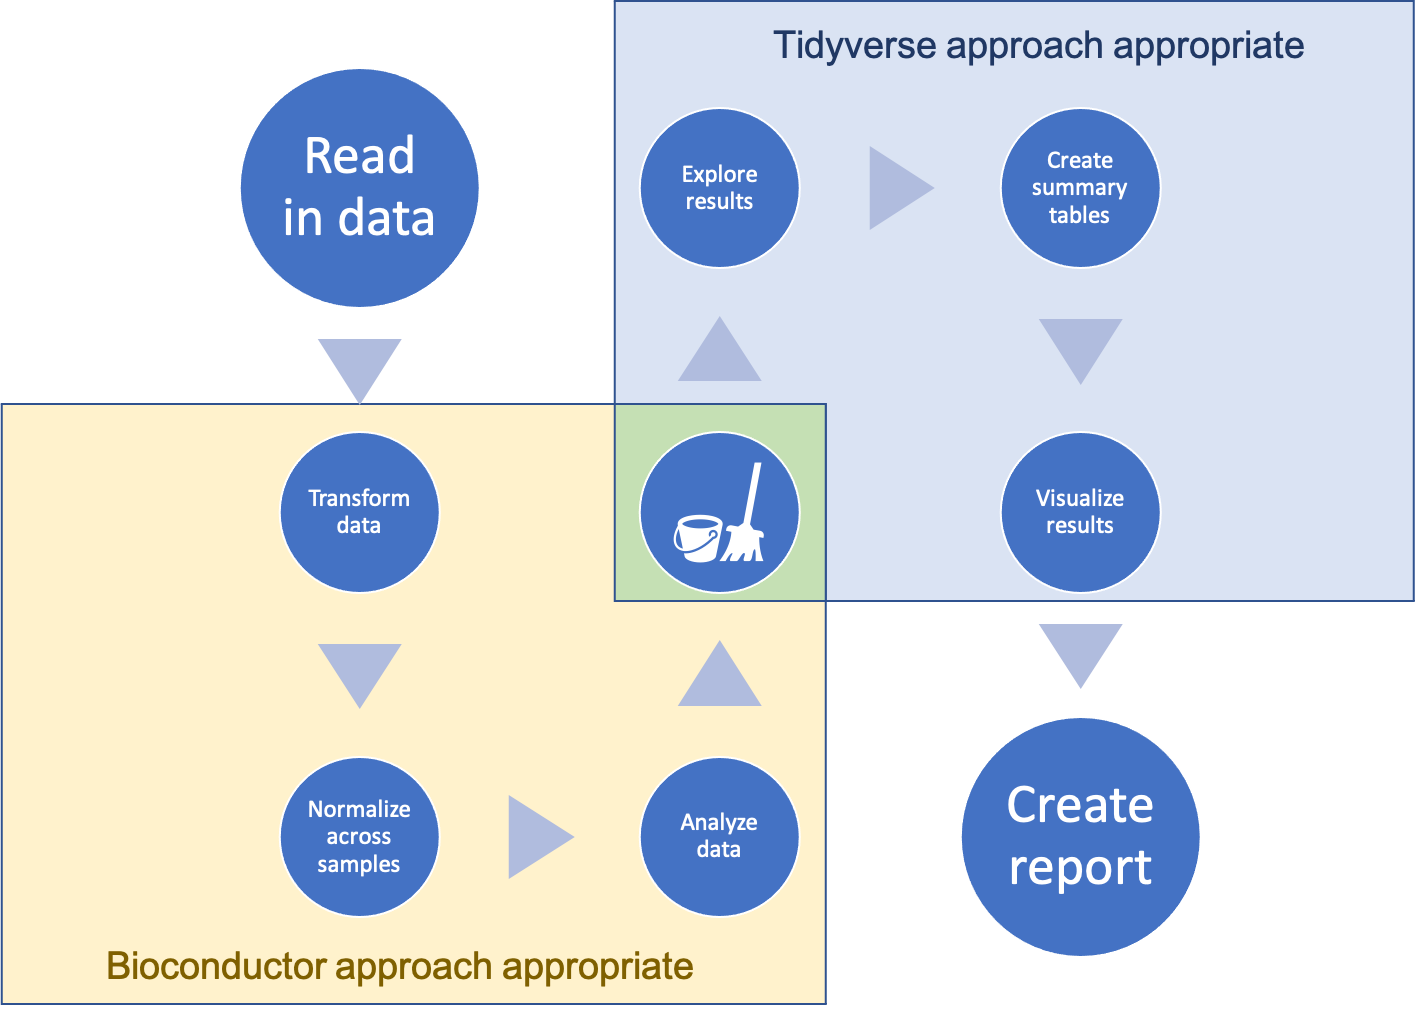
\includegraphics[width=\textwidth]{figures/workflow} \caption[An overview of a workflow that moves from a Bioconductor approach---for pre-processing of the data---through to a tidyverse approach one pre-processing has created smaller, simpler data that can be reasonably stored in a dataframe structure]{An overview of a workflow that moves from a Bioconductor approach---for pre-processing of the data---through to a tidyverse approach one pre-processing has created smaller, simpler data that can be reasonably stored in a dataframe structure.}\label{fig:combinedworkflow}
\end{figure*}

There are two key tools that have been developed as our packages that facilitate the shift of data from being stored in a more customized object-oriented class, for example one of the S4 type classes that we discussed when talking about complex data formats for Bioconductor. These packages move data from one of those storage containers into a tidy dataframe format. By doing this it moves the data into a format that is very easy to use in conjunction with the tidyverse tools and the tidyverse approach.

In this module we will focus specifically on the biobroom package. Of the two
packages this focuses specifically on moving data out of many of the common
bioconductor classes and into tidy dataframes. this package drawers and an
object-oriented approach in that it provides generic functions for extracting
data from many different object classes that are coming in by a conductor. You
will call the same function regardless of the class that the dad is in. If that
object class has a bio broom method for that generic function, then the function
will be able to extract parts of the data into a tidy data frame.

In this module we will also discuss another tool from the tidyverse, or rather a
tool that draws on the tiny verse approach, that can be easily used in
conjunction with biomedical data that has been processed using bioconductor
tools. This is a package called \texttt{ggbio} that facilitates the visualization of
biomedical data. It includes functions and Specialized gian's or geometrical
objects that are customized for some of the tasks that you might want to conduct
in visualizing biomedical data in r. by drawing on tools and an approach from
ggplot which is part of the tidyverse approach, these tools allow you to work
with this data while still leveraging the powerful visualization tools and
philosophy underlying the ggplot package.

Finally it is quite likely better purchase will continue to evolve through are,
and that in the future there might be tidy data frame format that are adaptable
enough to handle earlier stages in the data preprocessing. Tidy first dataframe
have already been adapted to enable them to include more complex types of data
within certain columns of the data frame any special list type column. This
functionality is being leveraged through the ffs package to an evil a tidy
approach to working with geographical data. This allows those who are working
with geographical data, for example data from shapefiles for creating Maps, to
use the standard tidyverse approaches while still containing complex data needed
for this geographical information. It seems very possible that similar
approaches may be adapted in the near future to allow for biomedical or genomic
data to be stored in a way that both accounts for complexity early and
pre-processing of these data but also allows for a more natural integration with
the wealth of powerful tools available through the tidyverse approach.

\hypertarget{the-biobroom-package}{%
\subsection{\texorpdfstring{The \texttt{biobroom} package}{The biobroom package}}\label{the-biobroom-package}}

The \texttt{biobroom} package includes three main generic functions (methods), which
can be used on a number of Bioconductor object classes. When applied to object
stored in one of these Bioconductor classes, these functions will extract part
of the data into a tidy dataframe format. In this format, it is easy to use the
tools from the tidyverse to further explore, analyze, and visualize the data.

The three generic functions of \texttt{biobroom} are the functions \texttt{tidy}, \texttt{augment},
and \texttt{glance}. These function names mimic the names of the three main functions
in the \texttt{broom} package, which is a more general purpose package for extracting
tidy datasets from more complex R object containers. The \texttt{broom} package
focuses on the output from functions in R for statistical testing and modeling,
while the newer \texttt{biobroom} package replicates this idea, but for many of the
common object classes used to store data through Bioconductor packages and
workflows.

The \texttt{biobroom} package includes methods for the following object classes
\citep{biobroom}:

\begin{itemize}
\tightlist
\item
  \texttt{qvalue} objects, which are used \ldots{}
\item
  \texttt{DESeqDataSet} objects, which are used \ldots{}
\item
  \texttt{DGEExact} objects, which are used \ldots{}
\item
  {[}limma objects{]}
\item
  {[}ExpressoinSet objects{]}
\item
  \texttt{MSnSet} objects, which are used \ldots{}
\end{itemize}

As an example, we can look at how the \texttt{biobroom} package can be used to
convert output generated by functions in the \texttt{edgeR} package into a tidy
dataframe, and how that output can then be explored and visualized using
functions from the tidyverse.

The \texttt{edgeR} package is a popular Bioconductor package that can be used on gene
expression data to explore which genes are expressed differently across
experimental groups (\emph{differential expression analysis}) \citep{edgeR}. Before using
the functions in the package, the data must be preprocessed to align sequence
reads from the raw data and then to create a table with the counts of each read
at each gene across each sample. The \texttt{edgeR} package includes functions for
pre-processing through its own functions, as well, including capabilities for
filtering out genes with low read counts across all samples and model-based
normalization across samples to help handle technical bias, including
differences in sequencing depth \citep{chen2014edger}.

The \texttt{edgeR} package operates on data stored in a special object class
defined by the package, the \texttt{DGEList} object class \citep{chen2014edger}.
This object class includes areas for storing the table of read counts,
in the form of a matrix appropriate for analysis by other functions in
the package, as well as other spots for storing information about each
sample and, if needed, a space to store annotations of the genes
\citep{chen2014edger}.

{[}Example from the \texttt{biobroom} help documentation---uses the \texttt{hammer} data
that comes with the package. These data are stored in an \texttt{ExpressionSet}
object, an object class defined by the \texttt{Biobase} package. You can see how the \texttt{tidy} function extracts these data in a
tidy format. Then, the data are put in a \texttt{DGEList} class so they are in
the right container for operations from \texttt{edgeR}. Then functions from the
\texttt{edgeR} package are run to perform differential expression analysis on the
data. The result is an object in the \texttt{DGEExact} class, which is defined
by the \texttt{edgeR} package. To extract data from this class in a tidy format,
you can use the \texttt{tidy} and \texttt{glance} functions from \texttt{biobroom}.{]}

\begin{Shaded}
\begin{Highlighting}[]
\FunctionTok{library}\NormalTok{(biobroom)}
\FunctionTok{library}\NormalTok{(Biobase)}
\FunctionTok{library}\NormalTok{(edgeR)}

\FunctionTok{data}\NormalTok{(hammer)}

\FunctionTok{class}\NormalTok{(hammer)}
\end{Highlighting}
\end{Shaded}

\begin{verbatim}
## [1] "ExpressionSet"
## attr(,"package")
## [1] "Biobase"
\end{verbatim}

\begin{Shaded}
\begin{Highlighting}[]
\FunctionTok{tidy}\NormalTok{(hammer)}
\end{Highlighting}
\end{Shaded}

\begin{verbatim}
## # A tibble: 236,128 x 3
##    gene               sample    value
##    <chr>              <chr>     <int>
##  1 ENSRNOG00000000001 SRX020102     2
##  2 ENSRNOG00000000007 SRX020102     4
##  3 ENSRNOG00000000008 SRX020102     0
##  4 ENSRNOG00000000009 SRX020102     0
##  5 ENSRNOG00000000010 SRX020102    19
##  6 ENSRNOG00000000012 SRX020102     7
##  7 ENSRNOG00000000014 SRX020102     0
##  8 ENSRNOG00000000017 SRX020102     4
##  9 ENSRNOG00000000021 SRX020102     7
## 10 ENSRNOG00000000024 SRX020102    86
## # ... with 236,118 more rows
\end{verbatim}

\begin{Shaded}
\begin{Highlighting}[]
\DocumentationTok{\#\# Example from \textasciigrave{}biobroom\textasciigrave{} help documentation}
\NormalTok{hammer.counts }\OtherTok{\textless{}{-}} \FunctionTok{exprs}\NormalTok{(hammer)[, }\DecValTok{1}\SpecialCharTok{:}\DecValTok{4}\NormalTok{]}
\NormalTok{hammer.treatment }\OtherTok{\textless{}{-}} \FunctionTok{phenoData}\NormalTok{(hammer)}\SpecialCharTok{$}\NormalTok{protocol[}\DecValTok{1}\SpecialCharTok{:}\DecValTok{4}\NormalTok{]}

\NormalTok{y }\OtherTok{\textless{}{-}} \FunctionTok{DGEList}\NormalTok{(}\AttributeTok{counts=}\NormalTok{hammer.counts,}\AttributeTok{group=}\NormalTok{hammer.treatment)}
\NormalTok{y }\OtherTok{\textless{}{-}} \FunctionTok{calcNormFactors}\NormalTok{(y)}
\NormalTok{y }\OtherTok{\textless{}{-}} \FunctionTok{estimateCommonDisp}\NormalTok{(y)}
\NormalTok{y }\OtherTok{\textless{}{-}} \FunctionTok{estimateTagwiseDisp}\NormalTok{(y)}
\NormalTok{et }\OtherTok{\textless{}{-}} \FunctionTok{exactTest}\NormalTok{(y)}

\FunctionTok{class}\NormalTok{(et)}
\end{Highlighting}
\end{Shaded}

\begin{verbatim}
## [1] "DGEExact"
## attr(,"package")
## [1] "edgeR"
\end{verbatim}

\begin{Shaded}
\begin{Highlighting}[]
\FunctionTok{tidy}\NormalTok{(et)}
\end{Highlighting}
\end{Shaded}

\begin{verbatim}
## # A tibble: 29,516 x 4
##    gene               estimate  logCPM    p.value
##    <chr>                 <dbl>   <dbl>      <dbl>
##  1 ENSRNOG00000000001   2.65    1.49   0.00000131
##  2 ENSRNOG00000000007  -0.409  -0.226  1         
##  3 ENSRNOG00000000008   2.22   -0.407  0.129     
##  4 ENSRNOG00000000009   0      -1.31   1         
##  5 ENSRNOG00000000010   0.0331  1.79   1         
##  6 ENSRNOG00000000012  -3.39    0.0794 0.00375   
##  7 ENSRNOG00000000014   3.65   -0.854  0.252     
##  8 ENSRNOG00000000017   2.42    1.11   0.0000638 
##  9 ENSRNOG00000000021  -2.02    0.211  0.0373    
## 10 ENSRNOG00000000024   0.133   3.97   0.508     
## # ... with 29,506 more rows
\end{verbatim}

\begin{Shaded}
\begin{Highlighting}[]
\FunctionTok{glance}\NormalTok{(et)}
\end{Highlighting}
\end{Shaded}

\begin{verbatim}
##   significant     comparison
## 1        6341 control/L5 SNL
\end{verbatim}

The creator of the \texttt{broom} package listed some of the common ways that
statistical model output objects---the focus on `tidying' in \texttt{broom}---tend to
be untidy. These include that important information is stored in the row names,
where it is harder to access, that the names of some columns can be tricky to
work with because they use non-standard conventions (i.e., they don't follow the
rules for naming objects in R), that some desired information is not available
in the object, but rather is typically computed with later methods for the
object, like when \texttt{summary} is run on the object, or are only available as the
result of a \texttt{print} method run on the object, and vectors that a user may want
to explore in tandem are stored in different places in the object.
\citep{robinson2014broom}

{[}Examples of these in Bioconductor objects?{]}

These `messy' characteristics show up in the data stored in Bioconductor
objects, as well, in terms of characteristics that impede working with
data stored in these formats easily using tools from the tidyverse.
As an example, one common class for storing data in Bioconductor work is
the \texttt{ExpressionSet} object class, defined in the \texttt{Biobase} package \citep{biobase}.
This object class can be used to store the data from high-throughput
assays. It includes slots for the assay data, as well as slots
for storing metadata about the experiment, which could include information
like sampling time points or sample strains, as well as the experimental
group of each sample (control versus treated, for example).

Data from the assay for the experiment---for example, gene expression
or intensity {[}?{]} measurements for each gene and each sample {[}?{]}---can be
extracted from an \texttt{ExpressionSet} object using an extractor function
called \texttt{exprs}. Here is an example using the \texttt{hammer} example dataset
available with the \texttt{biobroom} package. The code call here extracts the
assay data from the \texttt{hammer} R object, which is an instance of the
\texttt{ExpressionSet} object class. It uses indexing (\texttt{{[}1:10,\ 1:3{]}}) to limit
printing to the first ten rows and first three columns of the output, so
we can investigate a small snapshot of the data:

\begin{verbatim}
##                    SRX020102 SRX020103 SRX020104
## ENSRNOG00000000001         2         4        18
## ENSRNOG00000000007         4         1         3
## ENSRNOG00000000008         0         1         4
## ENSRNOG00000000009         0         0         0
## ENSRNOG00000000010        19        10        19
## ENSRNOG00000000012         7         5         1
## ENSRNOG00000000014         0         0         2
## ENSRNOG00000000017         4         1        12
## ENSRNOG00000000021         7         5         2
## ENSRNOG00000000024        86        53        86
\end{verbatim}

These data are stored in a matrix format. The gene identifiers {[}?{]} are given in
the rownames and the samples in the column names. Each cell of the matrix
provides the expression level (number of reads {[}?{]}) of a specific gene in a
specific sample.

These data are structured and stored in such a way that they have some of the
characteristics that can make data difficult to work with the data using
tidyverse tools. For example, they store gene identifiers in the rownames,
rather than in a separate column where they can be easily accessed when using
tidyverse functions. Also, there are phenotype / meta data that are stored
in other parts of the \texttt{ExpressionSet} data but that may be interesting to
explore in conjunction with these assay data, including the experimental
group of each sample (control versus animals in which chronic neuropathic
pain was induced, in these example data).

The \texttt{tidy} function from the \texttt{biobroom} package extracts these data and
restructures them into a `tidy' format, ready to use easily with tidyverse
tools.

\begin{verbatim}
## # A tibble: 236,128 x 3
##    gene               sample    value
##    <chr>              <chr>     <int>
##  1 ENSRNOG00000000001 SRX020102     2
##  2 ENSRNOG00000000007 SRX020102     4
##  3 ENSRNOG00000000008 SRX020102     0
##  4 ENSRNOG00000000009 SRX020102     0
##  5 ENSRNOG00000000010 SRX020102    19
##  6 ENSRNOG00000000012 SRX020102     7
##  7 ENSRNOG00000000014 SRX020102     0
##  8 ENSRNOG00000000017 SRX020102     4
##  9 ENSRNOG00000000021 SRX020102     7
## 10 ENSRNOG00000000024 SRX020102    86
## # ... with 236,118 more rows
\end{verbatim}

This output is a tidy dataframe object, with three columns providing the
gene name, the sample identifier, and the expression level. In this format,
the data can easily be explored and visualized with tidyverse tools. For example,
you could easily create a set of histograms, one per sample, showing the
distribution of expression levels across all genes in each sample:
{[}better example visualization here?{]}

\begin{verbatim}
## `stat_bin()` using `bins = 30`. Pick better value with `binwidth`.
\end{verbatim}

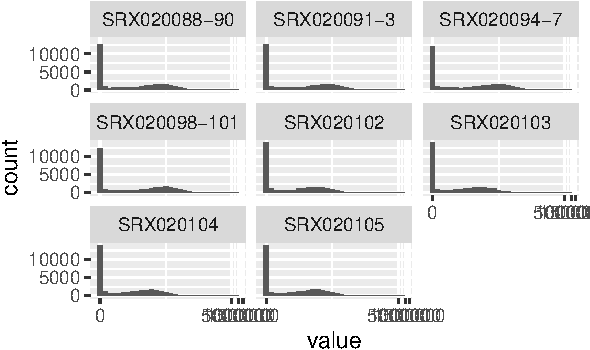
\includegraphics{improve_repro_files/figure-latex/unnamed-chunk-22-1}

You can also incorporate data that are stored in the \texttt{phenoData} slot of
the \texttt{ExpressionSet} object by specifying \texttt{addPheno\ =\ TRUE}:

\begin{verbatim}
## # A tibble: 236,128 x 8
##    gene               sample sample.id num.tech.reps protocol strain Time  value
##    <chr>              <chr>  <fct>             <dbl> <fct>    <fct>  <fct> <int>
##  1 ENSRNOG00000000001 SRX02~ SRX020102             1 control  Sprag~ 2 mo~     2
##  2 ENSRNOG00000000007 SRX02~ SRX020102             1 control  Sprag~ 2 mo~     4
##  3 ENSRNOG00000000008 SRX02~ SRX020102             1 control  Sprag~ 2 mo~     0
##  4 ENSRNOG00000000009 SRX02~ SRX020102             1 control  Sprag~ 2 mo~     0
##  5 ENSRNOG00000000010 SRX02~ SRX020102             1 control  Sprag~ 2 mo~    19
##  6 ENSRNOG00000000012 SRX02~ SRX020102             1 control  Sprag~ 2 mo~     7
##  7 ENSRNOG00000000014 SRX02~ SRX020102             1 control  Sprag~ 2 mo~     0
##  8 ENSRNOG00000000017 SRX02~ SRX020102             1 control  Sprag~ 2 mo~     4
##  9 ENSRNOG00000000021 SRX02~ SRX020102             1 control  Sprag~ 2 mo~     7
## 10 ENSRNOG00000000024 SRX02~ SRX020102             1 control  Sprag~ 2 mo~    86
## # ... with 236,118 more rows
\end{verbatim}

With this addition, visualizations can easily be changed to also show the
experimental group of each sample:

\begin{verbatim}
## `stat_bin()` using `bins = 30`. Pick better value with `binwidth`.
\end{verbatim}

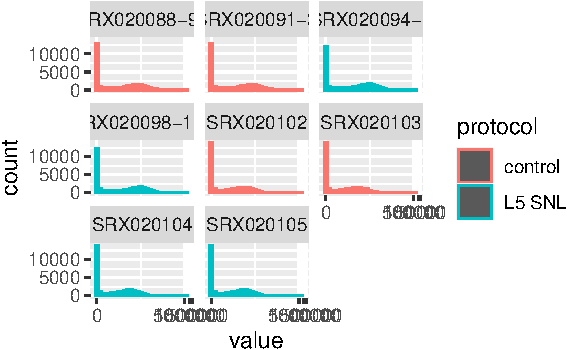
\includegraphics{improve_repro_files/figure-latex/unnamed-chunk-24-1}
You can also do things like look at differences in values for
specific genes, pairing tools for exploring data with tools for
visualization, both from the tidyverse:

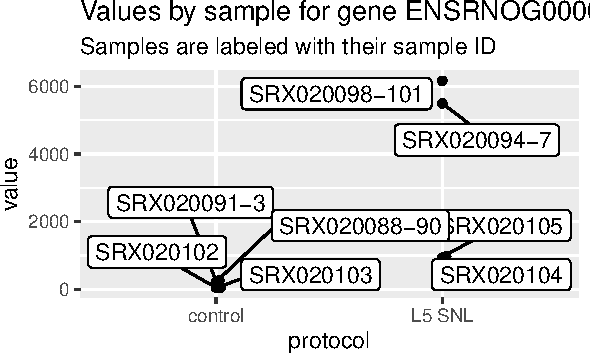
\includegraphics{improve_repro_files/figure-latex/unnamed-chunk-25-1}

The data for a subset of the sample can be analyzed using functions from the
\texttt{edgeR} package, to complete needed pre-processing (for example, calculating
normalizing factors with \texttt{calcNormFactors}, to reduce impacts from technical
bias {[}?{]}), estimate dispersion using conditional maximum likelihood and
empirical Bayesian methods (\texttt{estimateCommonDisp} and \texttt{estimateTagwiseDisp}), and
then perform a statistical analysis, conducting a differential expression
analysis (\texttt{exactTest}) \citep{chen2014edger}.

The data are stored in a special Bioconductor class, as an instance of
\texttt{DGEList}, throughout most of this process. This special class can be initialized
with data from the original \texttt{ExpressionSet} object, specifically, assay
data with the counts per gene in each sample and data on the experimental
phenotypes for the experiment---specifically, the protocol for each sample,
in terms of whether it was a control or if the sample was from an animal
in which chronic neuropathic pain was induced \citep{hammer2010mrna}.

\begin{verbatim}
## [1] "DGEList"
## attr(,"package")
## [1] "edgeR"
\end{verbatim}

Once the data are stored in this special \texttt{DGEList} class, different
steps of the preprocessing can be conducted. In each case, the results are
stored in special slots of the \texttt{DGEList} object. In this way, the original
data and results from preprocessing are all kept together in a single
object, each in a special slot within the object's structure.

\begin{verbatim}
## [1] "DGEList"
## attr(,"package")
## [1] "edgeR"
\end{verbatim}

\begin{verbatim}
## [1] "DGEList"
## attr(,"package")
## [1] "edgeR"
\end{verbatim}

\begin{verbatim}
## [1] "DGEList"
## attr(,"package")
## [1] "edgeR"
\end{verbatim}

After the preprocessing, the data can be analyzed using the \texttt{exactText} function.
This inputs the data stored in a \texttt{DGEList} object and outputs results into
a different object class, a \texttt{DGEExact} class.

\begin{verbatim}
## [1] "DGEExact"
## attr(,"package")
## [1] "edgeR"
\end{verbatim}

The \texttt{DGEExact} class is defined by the \texttt{edgeR} package and was created
specifically to store the results from a differential expression analysis
\citep{chen2014edger}. It has slots for a dataframe giving the estimates of
differential change in expression across the experimental groups for each
gene, within a \texttt{table} slot. Again, in this output, gene identifiers are
stored as rownames---which makes them hard to access with tidyverse tools---rather
than in their own column:

\begin{verbatim}
##                          logFC      logCPM       PValue
## ENSRNOG00000000001  2.64635814  1.49216267 1.309933e-06
## ENSRNOG00000000007 -0.40869816 -0.22616605 1.000000e+00
## ENSRNOG00000000008  2.22296029 -0.40665547 1.288756e-01
## ENSRNOG00000000009  0.00000000 -1.31347471 1.000000e+00
## ENSRNOG00000000010  0.03307909  1.79448965 1.000000e+00
## ENSRNOG00000000012 -3.39210151  0.07939132 3.745676e-03
\end{verbatim}

The \texttt{DGEExact} object also has a slot that contains a vector with identifiers
for the two experimental groups that are being compared in the
differential expression analysis, under the slot \texttt{comparison}:

\begin{verbatim}
## [1] "control" "L5 SNL"
\end{verbatim}

There is also a space in this object class where information about each
gene can be stored, if desired.

Two \texttt{biobroom} methods are defined for the \texttt{DGEExact} object class, \texttt{glance}
and \texttt{tidy}. The \texttt{tidy} method extracts the results from the differential
experssion analysis, but moves these results into a dataframe where the
gene names are given their own column, rather than being stored in the
hard-to-access rownames:

\begin{verbatim}
## # A tibble: 29,516 x 4
##    gene               estimate  logCPM    p.value
##    <chr>                 <dbl>   <dbl>      <dbl>
##  1 ENSRNOG00000000001   2.65    1.49   0.00000131
##  2 ENSRNOG00000000007  -0.409  -0.226  1         
##  3 ENSRNOG00000000008   2.22   -0.407  0.129     
##  4 ENSRNOG00000000009   0      -1.31   1         
##  5 ENSRNOG00000000010   0.0331  1.79   1         
##  6 ENSRNOG00000000012  -3.39    0.0794 0.00375   
##  7 ENSRNOG00000000014   3.65   -0.854  0.252     
##  8 ENSRNOG00000000017   2.42    1.11   0.0000638 
##  9 ENSRNOG00000000021  -2.02    0.211  0.0373    
## 10 ENSRNOG00000000024   0.133   3.97   0.508     
## # ... with 29,506 more rows
\end{verbatim}

Now that the data are in this tidy format, tools from the tidyverse can
be easily applied. For example, you could use functions from the \texttt{dplyr}
package to see the genes for which the differential expression analysis
resulted in both a very low p-value and a large difference in expression
across the experimental groups:

\begin{verbatim}
## # A tibble: 803 x 4
##    gene               estimate logCPM   p.value
##    <chr>                 <dbl>  <dbl>     <dbl>
##  1 ENSRNOG00000013496     6.39   3.41 5.95e- 46
##  2 ENSRNOG00000001338     6.01   2.25 1.37e- 22
##  3 ENSRNOG00000020136     5.17   3.89 3.19e- 52
##  4 ENSRNOG00000018808     4.78   6.46 1.75e-169
##  5 ENSRNOG00000006151     4.43   2.99 2.39e- 30
##  6 ENSRNOG00000009768     4.40   7.83 5.57e-293
##  7 ENSRNOG00000030927    -4.29   2.45 6.32e- 23
##  8 ENSRNOG00000001476     4.25   3.76 1.45e- 47
##  9 ENSRNOG00000004805     4.05   6.64 2.51e-185
## 10 ENSRNOG00000014327     3.85   4.51 5.39e- 63
## # ... with 793 more rows
\end{verbatim}

Other exploratory analysis will also be straightforward with the data
using tidyverse tools, now that they are in a ``tidy'' format.

The \texttt{glance} method can also be applied to data that are stored in a
\texttt{DGEExact} class. In this case, the method will extract the names of the
experimental groups being compared (from the \texttt{comparison} slot of the
object) as well as count the number of genes with statistically
significant differences in expression level, based on the values in the
\texttt{table} slot of the object.

\begin{verbatim}
##   significant     comparison
## 1        6341 control/L5 SNL
\end{verbatim}

\begin{verbatim}
##   significant     comparison
## 1        4225 control/L5 SNL
\end{verbatim}

As another example, you can now use tools from \texttt{ggplot2}, as well as
extensions built on this package, to do things like create a volcano
plot of the data with highlighting of noteworthy genes on the plot:

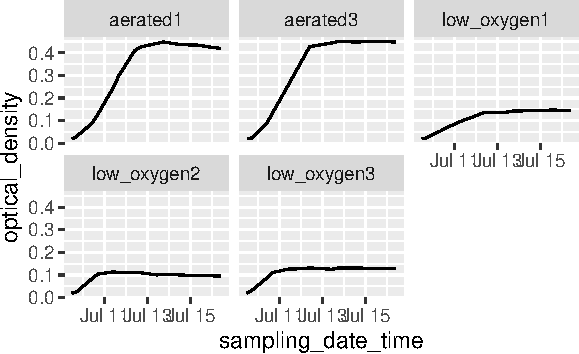
\includegraphics{improve_repro_files/figure-latex/unnamed-chunk-34-1}

If you wanted to access the help files for these \texttt{biobroom} methods for this
object class, you could do so by calling help in R (\texttt{?}) using the name of the
method, a dot, and then the name of the object class, e.g., \texttt{?tidy.DGEExact}.

\hypertarget{the-ggbio-package}{%
\subsection{\texorpdfstring{The \texttt{ggbio} package}{The ggbio package}}\label{the-ggbio-package}}

\hypertarget{subsection-2-4}{%
\subsection{Subsection 2}\label{subsection-2-4}}

\begin{quote}
``The biobroom package contains methods for converting standard objects in Bioconductor into a `tidy format'. It serves as a complement to the popular broom package, and follows the same division (tidy/augment/glance) of tidying methods.''
\citep{biobroom}
\end{quote}

\begin{quote}
``Tidying data makes it easy to recombine, reshape and visualize bioinformatics analyses. Objects that can be tidied include: ExpressionSet object,
GRanges and GRangesList objects, RangedSummarizedExperiment object, MSnSet object,
per-gene differential expression tests from limma, edgeR, and DESeq2, qvalue object for multiple hypothesis testing.'' \citep{biobroom}
\end{quote}

\begin{quote}
``We are currently working on adding more methods to existing Bioconductor objects.'' \citep{biobroom}
\end{quote}

\begin{quote}
``All biobroom tidy and augment methods return a tbl\_df by default (this prevents them from printing many rows at once, while still acting like a traditional data.frame).'' \citep{biobroom}
\end{quote}

\begin{quote}
``The concept of `tidy data' offers a powerful framework for structuring data
to ease manipulation, modeling and visualization. However, most R functions,
both those builtin and those found in third-party packages, produce output that
is not tidy, and that is therefore difficult to reshape, recombine, and
otherwise manipulate. Here I introduce the broom package, which turns the output
of model objects into tidy data frames that are suited to further analysis,
manipulation, and visualization with input-tidy tools.'' \citep{robinson2014broom}
\end{quote}

\begin{quote}
``Tools are classified as `messy-output' if their output does not fit into this
{[}tidy{]} framework. Unfortunately, the majority of R modeling tools, both from the
built-in stats package and those in common third party packages, are
messy-output. This means the data analyst must tidy not only the original data,
but the results at each intermediate stage of an analysis.'' \citep{robinson2014broom}
\end{quote}

\begin{quote}
``The broom package is an attempt to solve this issue, by bridging the gap from
untidy outputs of predictions and estimations to create tidy data that is easy
to manipulate with standard tools. It centers around three S3 methods, tidy,
augment, and glance, that each take an object produced by R statistical
functions (such as lm, t.test, and nls) or by popular third-party packages (such
as glmnet, survival, lme4, and multcomp) and convert it into a tidy data frame
without rownames (Friedman et al., 2010; Therneau, 2014; Bates et al., 2014;
Hothorn et al., 2008). These outputs can then be used with input-tidy tools such
as dplyr or ggplot2, or downstream statistical tests. broom should be
distinguished from packages such as reshape2 and tidyr, which rearrange and
reshape data frames into different forms (Wickham, 2007b, 2014b). Those packages
perform essential tasks in tidy data analysis but focus on manipulating data
frames in one specific format into another. In contrast, broom is designed to
take data that is not in a data frame (sometimes not anywhere close) and convert
it to a tidy data frame.'' \citep{robinson2014broom}
\end{quote}

\begin{quote}
``\texttt{tidy} constructs a data frame that summarizes the model's statistical
components, which we refer to as the component level. In a regression such as
the above it may refer to coefficient estimates, p-values, and standard errors
for each term in a regression. The tidy generic is flexible- in other models it
could represent per-cluster information in clustering applications, or per-test
information for multiple comparison functions. \ldots{} \texttt{augment} add columns to the
original data that was modeled, thus working at the observation level. This
includes predictions, residuals and prediction standard errors in a regression,
and can represent cluster assignments or classifications in other applications.
By convention, each new column starts with . to ensure it does not conflict with
existing columns. To ensure that the output is tidy and can be recombined,
rownames in the original data, if present, are added as a column called
.rownames. \ldots{} Finally, \texttt{glance} constructs a concise one-row summary of the
model level values. In a regression this typically contains values such as R2 ,
adjusted R2 , residual standard error, Akaike Information Criterion (AIC), or
deviance. In other applications it can include calculations such as cross
validation accuracy or prediction error that are computed once for the entire
model. \ldots{} These three methods appear across many analyses; indeed, the fact
that these three levels must be combined into a single S3 object is a common
reason that model outputs are not tidy. Importantly, some model objects may have
only one or two of these methods defined. (For example, there is no sense in
which a Student's T test or correlation test generates information about each
observation, and therefore no augment method exists).'' \citep{robinson2014broom}
\end{quote}

\begin{quote}
``While model inputs usually require tidy inputs, such attention to detail
doesn't carry over to model outputs. Outputs such as predictions and estimated
coefficients aren't always tidy. For example, in R, the default representation
of model coefficients is not tidy because it does not have an explicit variable
that records the variable name for each estimate, they are instead recorded as
row names. In R, row names must be unique, so combining coefficients from many
models (e.g., from bootstrap resamples, or subgroups) requires workarounds to
avoid losing important information. This knocks you out of the flow of analysis
and makes it harder to combine the results from multiple models.''
\citep{wickham2014tidy}
\end{quote}

\begin{quote}
``edgeR can be applied to differential expression at the gene, exon, transcript
or tag level. In fact, read counts can be summarized by any genomic feature.
edgeR analyses at the exon level are easily extended to detect differential
splicing or isoform-specific differential expression.'' \citep{chen2014edger}
\end{quote}

\begin{quote}
``edgeR provides statistical routines for assessing differential expression in
RNA-Seq experiments or differential marking in ChIP-Seq experiments. The package
implements exact statistical methods for multigroup experiments developed by
Robinson and Smyth {[}33, 34{]}. It also implements statistical methods based on
generalized linear models (glms), suitable for multifactor experiments of any
complexity, developed by McCarthy et al.~{[}22{]}, Lund et al.~{[}20{]}, Chen et al.~{[}5{]}
and Lun et al.~{[}19{]}. \ldots{} A particular feature of edgeR functionality, both
classic and glm, are empirical Bayes methods that permit the estimation of
gene-specific biological variation, even for experiments with minimal levels of
biological replication.'' \citep{chen2014edger}
\end{quote}

\begin{quote}
``edgeR performs differential abundance analysis for pre-defined genomic
features. Although not strictly necessary, it usually desirable that these
genomic features are non-overlapping. For simplicity, we will hence-forth refer
to the genomic features as `genes', although they could in principle be
transcripts, exons, general genomic intervals or some other type of feature. For
ChIP-seq experiments, abundance might relate to transcription factor binding or
to histone mark occupancy, but we will henceforth refer to abundance as in terms
of gene expression.'' \citep{chen2014edger}
\end{quote}

\begin{quote}
``edgeR stores data in a simple list-based data object called a DGEList. This
type of object is easy to use because it can be manipulated like any list in R.
\ldots{} The main components of an DGEList object are a matrix counts containing the
integer counts, a data.frame samples containing information about the samples or
libraries, and a optional data.frame genes containing annotation for the genes
or genomic features. The data.frame samples contains a column lib.size for the
library size or sequencing depth for each sample. If not specified by the user,
the library sizes will be computed from the column sums of the counts. For
classic edgeR the data.frame samples must also contain a column group,
identifying the group membership of each sample.'' \citep{chen2014edger}
\end{quote}

\begin{quote}
``Genes with very low counts across all libraries provide little evidence for
differential expression. In the biological point of view, a gene must be
expressed at some minimal level before it is likely to be translated into a
protein or to be biologically important. In addition, the pronounced
discreteness of these counts interferes with some of the statistical
approximations that are used later in the pipeline. These genes should be
filtered out prior to further analysis. As a rule of thumb, genes are dropped if
they can't possibly be expressed in all the samples for any of the conditions.
Users can set their own definition of genes being expressed. Usually a gene is
required to have a count of 5-10 in a library to be considered expressed in that
library. Users should also filter with count-per-million (CPM) rather than
filtering on the counts directly, as the latter does not account for differences
in library sizes between samples.'' \citep{chen2014edger}
\end{quote}

\begin{quote}
``The most obvious technical factor that affects the read counts {[}in data for
edgeR and so requires normalizations{]}, other than gene expression levels, is the
sequencing depth of each RNA sample. edgeR adjusts any differential expression
analysis for varying sequencing depths as represented by differing library
sizes. This is part of the basic modeling procedure and flows automatically into
fold-change or p-value calculations. It is always present, and doesn't require
any user intervention.'' \citep{chen2014edger}
\end{quote}

\begin{quote}
``In edgeR, normalization takes the form of correction factors that enter into
the statistical model. Such correction factors are usually computed internally
by edgeR functions, but it is also possible for a user to supply them. The
correction factors may take the form of scaling factors for the library sizes,
such as computed by calcNormFactors, which are then used to compute the
effective library sizes. Alternatively, gene-specific correction factors can be
entered into the glm functions of edgeR as offsets. In the latter case, the
offset matrix will be assumed to account for all normalization issues, including
sequencing depth and RNA composition. Note that normalization in edgeR is
model-based, and the original read counts are not themselves transformed. This
means that users should not transform the read counts in any way before inputing
them to edgeR.'' \citep{chen2014edger}
\end{quote}

\begin{quote}
``Recent work on a grammar of graphics could be extended for biological
data. The grammar of graphics is based on modular components that when
combined in different ways will produce different graphics. This enables
the user to construct a cominatoric number of plots, including those that
were not preconceived by the implementation of the grammar. Most existing
tools lack these capabilities.'' \citep{yin2012ggbio}
\end{quote}

\begin{quote}
``A new package, ggbio, has been developed and is available on Bioconductor.
The package provides the tools to create both typical and non-typical
biological plots for genomic data, generated from core Bioconductor data
structures by either the high-level autoplot function, or the
combination of low-level components of the grammar of graphics. Sharing
data structures with the rest of Bioconductor enables direct integration
with Bioconductor workflows.'' \citep{yin2012ggbio}
\end{quote}

\begin{quote}
``In ggbio, most of the functionality is available through a single
command, autoplot, which recognizes the data structure and makes a best
guess of the appropriate plot. \ldots{} Compared to the more general qplot
API of ggplot2, autoplot facilitates the creation of specialized biological
graphics and reacts to the specific class of object passed to it. Each type
of object has a specific set of relevant graphical parameters, and further
customization is possible through the low-level API.'' \citep{yin2012ggbio}
\end{quote}

The \texttt{ggbio} package has \texttt{autoplot} functions for many Bioconductor object
classes, including \texttt{GRangesList}, \ldots{} {[}\citet{yin2012ggbio}

\begin{quote}
``The grammar {[}of graphics{]} is composed of interchangeable components
that are combined according to a flexible set of rules to produce plots
from a wide range of types.'' \citep{yin2012ggbio}
\end{quote}

\begin{quote}
``Data are the first component of the grammar\ldots{} The ggbio package attempts
to automatically load files of specific formats into common Bioconductor
data structures, using routines provided by Bioconductor packages\ldots{}
The type of data structure loaded from a file or returned by an algorithm
depends on the intrinsic structure of the data. For example, BAM files are
loaded into a GappedAlignments, while FASTA and 2bit sequences result in
a DNAStringSet. The ggbio package handles each type of data structure
differently\ldots{} In summary, this abstraction mechanism allows ggbio to
handle multiple file formats, without discarding any intrinsic properties
that are critical for effective plotting.'' \citep{yin2012ggbio}
\end{quote}

\begin{quote}
``Genomic data have some specific features that are different from those of
more conventional data types, and the basic grammar does not conveniently
capture such aspects. The grammar of graphics is extended by ggbio in
several ways\ldots{} These extensions are specific to genomic data, that is,
genomic sequences and features, like genes, located on those sequences.''
\citep{yin2012ggbio}
\end{quote}

\begin{quote}
``A geom is responsible for translating data to a visual, geometric
representation according to mappings between variables and aesthetic
properties on the geom. In comparison to regular data elements that
might be mapped to the ggplot2 geoms of points, lines, and polygons,
genomic data has the basic currency of a range. Ranges underlie exons,
introns, and other features, and the genomic coordinate system forms
the reference frame for biological data. We have introduced or extended
several geoms for representing ranges and gaps between ranges. \ldots{}
For example, the alignment geom delegates to two other geoms for drawing
the ranges and gaps. These default to rectangles and chevrons, respectively.
Having specialized geoms for commonly encountered entities, like genes,
relegates the tedious coding of primatives, and makes use code simpler
and more maintainable.'' \citep{yin2012ggbio}
\end{quote}

\begin{quote}
``Coordinate systems locate points in space, and we use coordinate
transformations to map from data coordinates to plot coordinates. The
most common coordinate system in statistical graphics is cartesian.
The transformation of data to cartesian coordinates involves mapping
points onto a plane specified by two perpendicular axes (x and y).
Why would two plots transform the coordinates differently for the same data?
The first reason is to simplify, such as changing curvilinear graphics to
linear, and the second reason is to reshape a graphic so that the most
important information jumps out at the viewer or can be more accurately
perceived. Coordinate transformations are also important in genomic data
visualization. For instance, features of interest are often small
compared to the intervening gaps, especially in gene models. The exons
are usually much smaller than the introns. If users are generally interested
in viewing exons and associated annotations, we could simply cut or
shrink the intervening introns to use the plot space efficiently.'' \citep{yin2012ggbio}
\end{quote}

\begin{quote}
``Almost all experimental outputs are associated with an experimental
design and other meta-data, for example, cancer types, gender, and age.
Faceting allows users to subset the data by a combination of factors and then
lay out multiple plots in a grid, to explore relationships between factors and
other variables. The ggplot2 package supports various types of faceting by
arbitrary factors. THe ggbio package extends this notion to facet by a list
of ranges of interest, for example, a list of gene regions. There is always
an implicit faceting by sequence (chromosome), because when the x axis is the
chromosomal coordinate, it is not sensible to plto data from different chromosomes
on the same plot.'' \citep{yin2012ggbio}
\end{quote}

\begin{quote}
``For custom use cases, ggbio provides a low-level API that maps more directly
to components of the grammar and thus expresses the plot more explicitly.
Generally speaking, we strive to provide sensible, overrideable defaults at the
high-level entry points, such as autoplot, while still supporting
customizability through the low-level API. All lower level functions have a
special prefix to indicate their role in the grammalr, like layout, geom,
stat, coord, and theme. The objects returned by the low-level API may be
added together via the conventional + syntax. This facilitates the creation of
new types of plots. A geom in ggplot2 may be extended to work with more
biological data model, for example, geom rect will automatically figure out the
boundary of rectangles when the data is a GRanges, as to geom bar, geom
segment, and so on.'' \citep{yin2012ggbio}
\end{quote}

\begin{quote}
``We use ggplot2 as the foundation for ggbio, due to its principled style,
intellegent defaults and explicit orientation towards the grammar of
graphics model.'' \citep{yin2012ggbio}
\citep{yin2012ggbio}
\end{quote}

\hypertarget{applied-exercise-6}{%
\subsection{Applied exercise}\label{applied-exercise-6}}

\hypertarget{module18}{%
\section{Introduction to reproducible data pre-processing protocols}\label{module18}}

Reproducibility tools can be used to create reproducible data pre-processing
protocols---documents that combine code and text in a `knitted' document, which
can be re-used to ensure data pre-processing is consistent and reproducible
across research projects. In this module, we will describe how reproducible data
pre-processing protocols can improve reproducibility of pre-processing
experimental data, as well as to ensure transparency, consistency, and
reproducibility across the research projects conducted by a research team.

\textbf{Objectives.} After this module, the trainee will be able to:

\begin{itemize}
\tightlist
\item
  Define a `reproducible data pre-processing protocol'
\item
  Explain how such protocols improve reproducibility at the data pre-processing
  phase
\item
  List other benefits, including improving efficiency and consistency of data
  pre-processing
\end{itemize}

\hypertarget{introducing-reproducible-data-pre-processing-protocols}{%
\subsection{Introducing reproducible data pre-processing protocols}\label{introducing-reproducible-data-pre-processing-protocols}}

\textbf{Data pre-processing}

When we take measurements of experimental samples, we do so with the goal of
using the data we collect to gain scientific knowledge. The data are direct
measurement of something, but need to be interpreted to gain knowledge.
Sometimes direct measurements line up very closely with a research
question---for example if you are conducting a study that investigates the
mortality status of each test subject then whether or not each subject to dies
is a data point that is directly related to the research question you are aiming
to answer. In this case these data may go directly into a statistical analysis
model without extensive pre-processing. However, there are often cases where we
collect data that are not as immediately linked to the scientific question.
Instead, these data may require pre-processing before they can be used to test
meaningful scientific hypotheses. This is often the case for data extracted
using complex equipment. Equipment like mass spectrometers and flow cytometers
leverage physics, chemistry, and biology in clever ways to help us derive more
information from samples, but one tradeoff is that the data from such equipment
often require a bit of work to move into a format that is useful for answering
scientific questions.

One example if the data collected through liquid chromatography-mass
spectrometry (LC-MS). This is a powerful and useful technique for chemical
analysis, including analysis of biochemical molecules like metabolites and
proteins. However, when using this technique, the raw data require extensive
pre-processing before they can be used to answer scientific questions.

First, the data that are output by the mass spectrometer are often stored in a
specialized file format, like a netCDF or mzML file format. While these file
formats are standardized, they are likely formats you don't regularly use in
other contexts, and so you may need to find special tools to read the data into
programs to analyze it. In some cases, the data are very large, and so it may be
necessary to use analysis tools that allow most of the data to stay ``on disk''
while you analyze it, bringing only small parts into your analysis software at a
time.

Once the data are read in, they must be pre-processed in a number of ways. For
example, these data can be translated into features that are linked to the
chemical composition of the sample, with each feature showing up as a ``peak'' in
the data that are output from the mass spectrometer. A peak can be linked to a
specific metabolite feature based on its mass-to-charge ratio (m/z) and its
retention time. However, the exact retention time for a metabolite feature may
vary a bit from sample to sample. Pre-processing is required both to identify
peaks in the data and also to align the peaks from the same metabolite feature
across all samples from your experiment. There may also be technical bias across
samples, resulting in differences in the typical expression levels of all peaks
from one sample to the next. For example it may be the case that all intensities
measured for one sample tend to be higher than for another sample because of
technical bias in terms of the settings used for the equipment when the two
samples were run. These biases must also be corrected through pre-processing
before you can use the data within statistical tests or models to explore scientific hypotheses.

{[}Image of identifying and aligning peaks in LC-MS data{]}

In the research process, these pre-processing steps should be done before
the data are used for further analysis. There are the first step in working
with the data after they are collected by the equipment (or by laboratory
personal, in the case of data from simpler process, like plating samples
and counting colony-forming units). After the data are appropriately
pre-processed, you can use them for statistical tests---for example, to
determine if metabolite profiles are different between experimental groups---and
also combine them with other data collected from the experiment---for example,
to see whether certain metabolite levels are correlated with the bacterial
load in a sample.

\textbf{Approaches for pre-processing data.}

There are two main approaches for pre-processing experimental data in this
way. First, when data are the output of complex laboratory equipment, there
will often be proprietary software that is available for this pre-processing.
This software may be created by the same company that made the equipment, or
it may be created and sold by other companies. The interface will typically
be a graphical-user interface (GUI), where you will use pull-down menus and
point-and-click interfaces to work through the pre-processing steps. You
often will be able to export a pre-processed version of the data in a
common file format, like a delimited file or an Excel file, and that version
of the data can then be read into more general data analysis software, like
Excel or R.

{[}Include a screenshot of this type of software in action.{]}

The second approach is to conduct the pre-processing directly within general
data analysis software like R or Python. These programs are both open-source,
and include extensions that were created and shared by users around the world.
Through these extensions, there are often powerful tools that you can use to
pre-process complex experimental data. In fact, the algorithms used in
proprietary software are sometimes extended from algorithms first shared through
R or Python. With this approach, you will read the data into the program (R,
for example) directly from the file output from the equipment. You can
record all the code that you use to read in and pre-process the data in a
code script, allowing you to reproduce this pre-processing work. You can
also go a step further, and incorporate your code into a pre-processing
protocol, which combines nicely formatted text with executable code, and
which we'll describe in much more detail later in this module and in the
following two modules.

There are advantages to taking the second approach---using scripted code in an
open-source program---rather than the first---using proprietary software with a
GUI interface. The use of codes scripts ensures that the steps of pre-processing
are reproducible. This means both that you will be able to re-do all the steps
yourself in the future, if you need to, but that also that other researchers can
explore and replicate what you do. You may want to share your process with
others in your laboratory group, for example, so they can understand the choices
you made and steps you took in pre-processing the data. You may also want to
share the process with readers of the articles you publish, and this may in fact
be required by the journal. Further, the use of a code script encourages you to
document this code and this process, even moreso when you move beyond a script
and include the code in a reproducible pre-processing protocol. Well-documented
code makes it much easier to write up the method section later in manuscripts
that leveraged the data collected in the experiment.

Also, when you use scripted code to pre-process biomedical data, you will find
that the same script can often be easily adapted and re-used in later projects
that use the same type of data. You may need to change small elements, like the
file names of files with data you want to use, or some details about the methods
used for certain pre-processing steps. However, often almost all of the
pre-processing steps will repeat over different experiments that you do. By
extending to write a pre-processing protocol, you can further support the
ease of adapting and re-using the pre-processing steps you take with one
experiment when you run later experiments that are similar.

\hypertarget{from-pre-processing-scripts-to-pre-processing-protocols}{%
\subsection{From pre-processing scripts to pre-processing protocols}\label{from-pre-processing-scripts-to-pre-processing-protocols}}

In the previous subsection, we mentioned that you can move a step beyond scripts
when pre-processing, and instead create a pre-processing protocol that includes
formatted text and executable code. This type of protocol can be easily created
using R, and it can serve as a reference for your laboratory group both of what
you did to pre-process data for the current experiment, but also as a starting
point for how to do similar analyses in the future. In module 3.9, we will walk
in detail through an example of this type of pre-processing protocol---you can
take a look now to get an idea by downloading the example
\href{https://github.com/geanders/improve_repro/raw/master/data/bactcountr_example_data/example_protocol.pdf}{here}.

This protocol includes all the code that was used for pre-processing, but it
isn't as limited as a simple code script with comments. Instead,

If you have used open-source software tools, like Bioconductor packages, you
are likely familiar with the \emph{vignettes} that come with the packages. These
provide tutorial guides showing you how to work with the package. They often
leverage example data that you can download so that you can try all the
example code yourself, before you move on to adapting the code to use with
your own data.

You can create your own version of these types of documents. This can use
real data from your research group, and you can create customized instructions
and code examples showing how to use open-source tools to pre-process a
certain type of biomedical data for experiments in your research group.
You can use this document the next time you need to pre-process that type
of data yourself, and you can also share it with others in your research
group. This can help in teaching new laboratory members how to work with
this type of data in your research group. It can also help ensure that
different members of the research group are all using the same steps to
pre-process data, so that there is greater consistency across results from
the group.

You may already create something similar to this, using a general word
processing program like Google Docs or Word. There are two key differences,
however, between how vignettes are created compared to a similar tutorial
created in Word or Google Docs. First, the vignettes are created using
a document compiling program that ensures that any code uses only ASCII
characters. This means that you can copy and paste code from the tutorial
into your R session and it will work. By contrast, programs like Word often
try to ``correct'' some of the characters when you paste in or type in code.
For example, when you have an apostrophe mark in your code (for example,
when you're quoting to create a character string), the computer code needs
to have this character as a very basic ASCII version of an apostrophe. Word,
by contrast, will often try to convert the character to use an apostrophe
character that looks smoother---and so is nice for a word processed document
that humans will read---but that R cannot recognize. Hyphens can have similar
problems. {[}Other examples?{]}

When you create a reproducible pre-processing protocol using the techniques that
are used to create vignettes---which we'll teach you how to do in the next few
sections---you will avoid this autocorrection of characters, and so someone
reading the protocol will be able to directly copy and paste example code from
the protocol into their own scripts. This will avoid hard-to-diagnose errors
that come from this character conversion in programs like Word.

The second difference is that the tools that are used to create vignettes
contain code that is not just copied and pasted from a script, but that is
actually, in essence, \emph{still in a script}. The code, in other words, is
executable and, unless you change the default settings, is re-run every
time you compile the document. This means that you will quickly determine if
there are any typos or other errors in the code, because the document will
not run and render correctly unless the code works. This means that you can
guarantee, when you first create the document, that the code runs, and also
that you can regularly check to see if the example code still works at
later time points. This allows you to, for example, see if changes in the
version of R or of specific packages that you're using has created problems
with the code running correctly over time.

Finally, these documents can be separated, allowing you to extract solely the
script part of the document, into a classic R script. You can use this directly
to run (or adapt) the pre-processing code for further research.

\hypertarget{technique-to-create-reproducible-pre-processing-protocols}{%
\subsection{Technique to create reproducible pre-processing protocols}\label{technique-to-create-reproducible-pre-processing-protocols}}

The vignettes that come with Bioconductor packages are created using a system
for ``knitting'' documents. These documents ``knit'' together text with executable
code. Once you have written the document, you can render it, which executes the
code, adds to the document results from this execution (figures, tables, and
code output, for example), and formats all text using the formatting choices
you've specified. The end result is a nicely format document, which can be in
one of several output formats, including pdf, Word, or HTML. Since the code
was executed to create the document, you can ensure that all the code
is worked as intended.

There are several techniques and principles that come together to make these
knitteed documents work. First are the tools that allow you to write text
in plain text, include formatting specifications in that plain text, and
render this to an attractive output document in pdf, Word, or HTML. This
part of the process uses a tool from a set of tools called \emph{Markup languages}.
{[}A bit more on history / development of Markup languages.{]}

Here, we will use a markup language called \emph{Markdown}. It is one of the easiest
markup languages to learn, as it has a fairly small set of formatting indicators
that can be used to ``markup'' the formatting in a document. This small set,
however, covers much of the formatting you might want to do, and so this
language provides an easy introduction to markup languages while still providing
adequate functionality for most purposes.

The Markdown markup languages evolved starting in spaces where people could
communicate in plain text only, without point-and-click methods for adding
formatting like bold or italic type \citep{buffalo2015bioinformatics}. For example,
early versions of email only allowed users to write using plain text. These
users eventually evolved some conventions for how to ``mark-up'' this plain text,
to serve the purposes served by things like italics and bold in formatted text
(e.g., emphasis, highlighting). For example, to emphasize a word, a user could
surround it with asterisks, like:

\begin{verbatim}
I just read a *really* interesting article!
\end{verbatim}

In this early prototype for a markup language, the reader's mind was doing
the ``rendering'', interpreting these markers as a sign that part of the text
was emphasized. In Markdown, the text can be rendered into more attractive
output documents, like pdf, where the rendering process has actually
changed the words between asterisks to print in italics.

The Markdown language has developed a set of these types of marks---like
asterisks---that are used to ``mark up'' the plain text with the formatting
that should be applied when the text is rendered. There are marks that you
can use for a number of formatting specifications, including: italics,
bold, underline, strike-through, bulleted lists, numbered lists, web links,
headers of different levels (e.g., to mark off sections and subsections),
block quotes, horizontal rules, and block quotes. Details and examples of
the Markdown syntax can be found on the Markdown Guide page at
\url{https://www.markdownguide.org/basic-syntax/}. We'll cover more examples of
using Markdown in the next two modules, as we move more specifically into
how RMarkdown can be used to created knitted documents with R and provide
an example of creating a reproducible protocol with this system.

The other technique that's needed to create knitted documents is the ability to
include executable code within the plain text version of the document, and to
execute that code and incorporate its results before moving on to render the
document to its final format.

The idea here is that you can use special markers to indicate in the document
where code starts and where it ends. With these markings, a computer program can
figure out the lines of the document that it should run as code, and the ones it
should ignore when it's looking for executable code. With these markings in
place, the document will be run through two separate programs as it is rendered.
The first program will look for code to execute and ignore any other lines of
the file. It will execute this code and then place any results, like figures,
tables, or code output, into the document right after that piece of code. The
output from running this program will then be input into a more traditional
markup renderer, which will format the document based on any of the mark up
indications and will output an attractive document in a format like pdf,
Word, or HTML.

This technique comes from an idea that you could include code to be executed in
a document that is otherwise easy for humans to read. This is an incrediably
powerful idea. It originated with a famous computer scientist named Donald
Knuth, who realized that one key to making computer code sound is to make sure
that it is clear to humans what the code is doing. Computers will faithfully do
exactly what you tell them to do, so they will do what you're hoping they will
as long as you provide the correct instructions. The greatest room for error,
then, comes from humans not giving the right instructions to computers. To
write sound code, and code that is easy for yourself and others to maintain and
extend, you must make sure that you and other humans understand what it is
asking the computer to do. Donald Knuth came up with a system called \emph{literate
programming} that allows programmers to write code in a way that focuses on
documenting the code for humans, while also allowing the computer to easily
pull out just the parts that it needs to execute, while ignoring all the text
meant for humans. This process flips the idea of documenting code by including
plain text comments in the code---instead of the code being the heart of the
document, the documentation of the code is the heart, with the code provided
to illustrate the implementation. When used well, this technique results in
beautiful documents that clearly and comprehensively document the intent and
the implementation of computer code. The knitted documents that we can build
with R or Python through systems like RMarkdown and Jupyter Notebooks build
on these literate programming ideas, applying them in ways that complement
programming languages that can be run interactively, rather than needing to
be compiled before they're run.

You can visualize the full process of creating and rendering a knitted document
in the following way. Imagine that you write a document by hand on sheets of
paper. There are parts where you need a team member to add their data or to run
a calculation, so you include notes in square brackets telling your team member
where to do these things. Then, you use traditional editing marks to show where
text should be italicized and which text should be section a header:

\begin{verbatim}
# Results

We measured the bacterial load of 
*Mycobacterium tuberculosis* for each 
sample. 

[Kristina: Calculate bacterial loads for 
each sample based on dilutions and
add table with results here.]
\end{verbatim}

This is analogous to writting up a knitted document in plain text with appropriate
``executable'' sections, designated with special markings, and with other markings
used to show how the text should be formatted in its final version.

You send the document to your team member first, and she does his calculations
and adds the results at the indicated spot in the paper. She focuses on the notes to
her in square brackets and ignores the rest of the document. This is analogous
to the first stage of rendering a knitted document, where the document is passed
through software that looks for executable code and ignores everything else,
executing that code and adding in results in the right place.

Next, your research team member sends the document, with her additions, to an
assistant to type up the document. The assistant types the full document, paying
attention to any indications that are included for formatting. For example, he
sees that ``Results'' is meant to be a section heading, since it is on a line that
starts with ``\#'', your team's convention for section headings. He therefore
types this on a line by itself in larger font. He also sees that ``Mycobacterium
tuberculosis'' is surrounded by asterisks, so he types this in italics. This
step is analogous to the second stage of rendering a formatted document, when
a software program takes the output of the first stage and formats the full
document into an attractive, easy-to-read final document, using any markings you
include to format the document.

\hypertarget{advantages-of-reproducible-pre-processing-protocols}{%
\subsection{Advantages of reproducible pre-processing protocols}\label{advantages-of-reproducible-pre-processing-protocols}}

With point-and-click software, even if you are doing the same process from one
experiment to another to pre-process your data, you will still have to go through
each step of preprocessing, re-selecting each choice along the way. For example,
if you are using software to gate flow cytometry data, someone in your research
group must typically go through the gating step-by-step, even if they are trying to
gate the data using the same rules and approach that they've applied to gate data
in previous experiments. This approach therefore has two key limitations.

First, it takes a lot of time for someone in the research group to go through
the same series of selection / point-and-click steps over and over each time
research data needs to be pre-processed. If steps do indeed need to be
customized extensively from one experiment to the next, there may be no way to
avoid this time-consuming work. However, if the same choices for pre-processing
apply from one experiment to the next, then there's not a good reason for
someone in the research group to need to spend a lot of time with this process.

Using a reproducible pre-processing protocol therefore helps make the
pre-processing more \textbf{efficient}. While developing this type of protocol will
take more time the first time or two that you do the pre-processing, as you
create, refine, and check the document, this time investment will pay off as you
continue to re-use the protocol in later experiments. Since the code can be
extracted as a script, you may find that you can often use that script as a
direct starting point for later experiments, needing only to change a few areas,
like the name of the input data files.

The second issue with a point-and-click approach is that it's hard to be sure
that you're being completely consistent from experiment to experiment if you're
going through the pre-processing ``by hand'', going through different steps and
selections using point-and-click software. Even if you've written down the
choices you plan to make from time to time, there may be subtle small choices
that you forget to write down. Further, there are some choices that might not be
as easy to make consistent from time to time. For example, when you gate flow
cytometry data using point and click software, you are often visual adjusting a
threshold or a box to select certain data points in the sample to gate. These
visual choices can be subjective from day to day, so you might gate the data
slightly different from one day to the next. Even if the same person does the
preprocessing from time to time, there will likely be subtle variations in the
process; these are likely to expand quite a bit when different people in the
research group do the pre-processing from one experiment to another.

By creating a reproducible pre-processing protocol, and starting from the
embedded code each time you pre-process data from a new experiment, you can
make your pre-processing more \textbf{reproducible} and more \textbf{consistent} from
one experiment to the next. When pre-processing is done using a code script,
the choices are based on an algorithm that can be reproduced faithfully from
experiment to experiment. For example, coding tools for gating flow cytometry
data use consistent algorithms, based on clear rules for fitting gates based
on the distribution of the data {[}?{]}, and so remove the subjectivity of
gating the data by hand, and the differences in gating that can result from
person to person or even from day to day in gating done by the same person.

In scientific research, there are numerous factors that can affect the
measurements that result from an experiment. These include differences across
experimental animals or subjects, differences in the set-up of different
laboratories, and so on. We often try to control as many extraneous factors as
we can, so that we can focus very precisely on how a single element affects an
outcome. By controlling extraneous factors, we can reduce the noise that might
obscure a signal in the relationship we care about and are trying to measure.
Subjectivity in data pre-processing is a potential source of noise in the
experimental process, especially for more complex biomedical data that requires
extensive pre-processing. Just as strong control to prevent variation in factors
like laboratory conditions and experimental animals can add power and clarity to
detect important signals in biomedical research, so can enforced consistency in
data pre-processing, including through the explicit use of consistent, objective
algorithms for pre-processing steps through the use of scripted code for as much
of the pre-processing as possible.

\hypertarget{what-knitted-documents-are-and-why-to-use-them}{%
\subsection{What knitted documents are and why to use them}\label{what-knitted-documents-are-and-why-to-use-them}}

If you have coded using a scripting language like R or Python, you likely have
already seen many examples of knitted documents. For both these languages, there
are many tutorials available that are created as knitted documents. Figure
\ref{fig:xcmsexample} shows an example from the start of a vignette for the
\texttt{xcms} package in R. This is a package that helps with pre-processing and
analyzing data from LC-MS experiments. You can see that this document includes
text to explain the package and also example code and the output from that code.

\begin{figure}
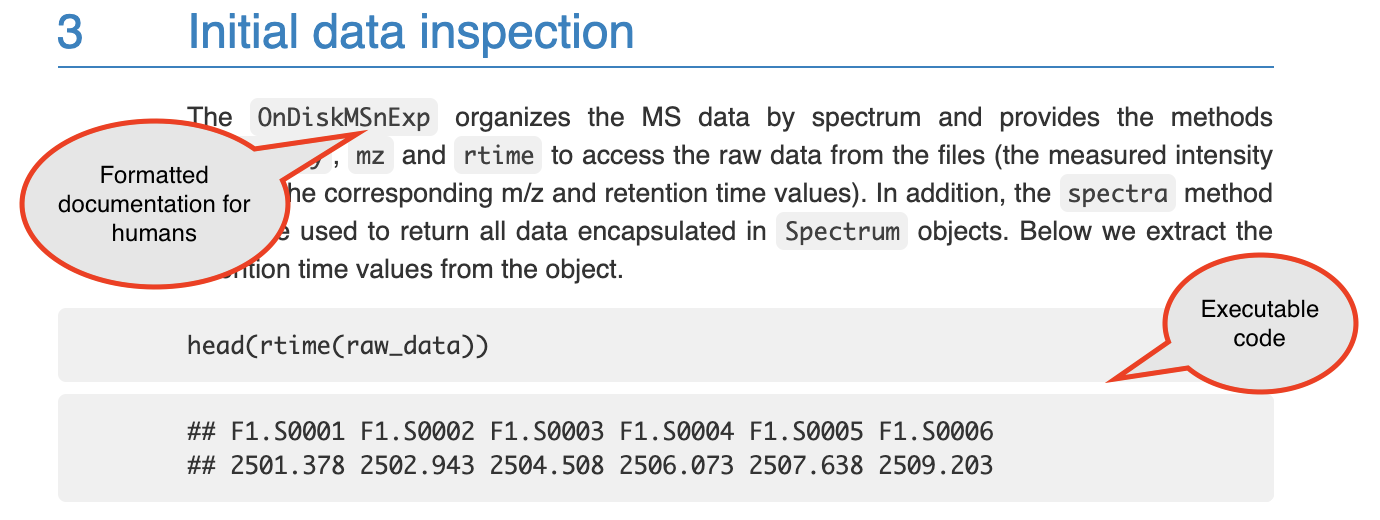
\includegraphics[width=\textwidth]{figures/vignette_example_annotated} \caption[An example of a knitted document]{An example of a knitted document. This shows a section of the online vignette for the `xcms` package from Bioconductor. The two types of content are highlighted: formatted text for humans to read, and executable computer code.}\label{fig:xcmsexample}
\end{figure}

As a larger example, all the modules in this online book were written as knitted
documents. In this module we will describe the characteristics of knitted
documents and how the technology behind them works. We will then talk about how
you can create them using Rmarkdown. In the next module, we'll provide an
example of doing this for a set of research data from a common laboratory
experiment.

The defining characteristic of a knitted document is that it interweaves two
types of content: first, executable code, and, second, documentation that is
formatted in a way that is easy to read. In the figure with the example from the
\texttt{xcms} vignette, we have highlighted the areas that demonstrate these two types
of content (Figure \ref{fig:xcmsexample}). Later in this module we will
describe how a knitted document can incorporate these two elements. First,
however, we will explain why you might want to use knitted documents to
document your own research code, especially for pre-processing protocols.

There are several advantages to using knitted documents when writing code to
pre-process or analyze research data. These include improvements in terms of
reliability, efficiency, transparency, and reproducibility.

First, when you have written your code within a knitted document, this code is
checked every time you render the document. In other words, you are checking
your code to ensure it operates as you intend throughout the process of writing
and editing your document, checking the code each time you render the document
to its formatted version. This helps to increase the \textbf{reliability} of the code
that you have written. Open-source software evolves over time, and by continuing
to check code as you work on protocols and reports with your data, you can
ensure that you will quickly identify and adapt to any such changes. Further,
you can quickly identify if updates to your research data introduce any issues
with the code. Again, by checking the code frequently, you can identify any
issues quickly, and this often will allow you to easily pinpoint and fix these
issues. By contrast, if you only identify a problem after writing a lot of code,
it is often difficult to identify the source of the issue. By including code
that is checked each time of document is rendered, you can quickly identify when
a change an open source software effects the analysis that you were conducting
or the pre-processing and work 2 adapt to any changes quickly.

Second, when you write a document that includes executable code, it allows you
to easily rerun the code as you update your research data set, or adopt the code
to work with a new data set. If you are not using a knitted document to write
pre-processing protocols and research reports, then your workflow is probably to
run all your code---either from a script or the command line---and copy the
results into a document in a word processing program like Word or Google Docs.
If you do that, you must recopy all your results every time you adapt any part
of the code or add new data. By contrast, when you use a knitted document, the
rendering process executes the code and incorporates the results directly and
automatically into a nicely formatted final document. The use of knitted
documents therefore can substantially improve the \textbf{efficiency} of
pre-processing and analyzing your data and generating the reports that summarize
this process.

Third, documents that are created in knitted format are created using plain
text. Plain text files can easily be tracked well and clearly using version
control tools like \emph{git}, and associated collaboration tools like GitHub, as
discussed in earlier modules. This substantially increases the \textbf{transparency}
of the data pre-processing and analysis. It allows you to clearly document
changes you or others make in the document, step-by-step. You can document who
made the change, and that person can include a message about why they made the
change. This full history of changes is recorded and can be searched to explore
how the document has evolved and why.

The final advantage of using knitted documents, especially for pre-processing
research data, is that it allows the code to be clearly and thoroughly
documented. This can help increase the \textbf{reproducibility} of the process. In
other words, it can help ensure that another researcher could repeat the same
process, making adaptations as appropriate for their own data set, or ensuring
they arrive at the same results if using the original data. It also ensures that
you can remember exactly what you did, which is especially useful if you plan to
reuse or adopt the code to work with other data sets, as will often be the case
for a pre-processing protocol. If you are not using a knitted document, but are
using code for preprocessing, then as an alternative you may be documenting your
code through comments in a code script. A code script does allow you to include
documentation about the code through these code comments, which are demarcated
from code in the script through a special symbol (\texttt{\#} in R). However these code
comments are much less expressive and harder to read than nicely formatted text,
and it is hard to include elements like mathematical equations and literature
citations in code comments. A knitted document allows you to write the
documentation in a format that is clear and attractive for humans to read, while
including code that is clear and easy for a computer to execute.

\hypertarget{how-knitted-documents-work}{%
\subsection{How knitted documents work}\label{how-knitted-documents-work}}

Next, we will describe how knitted documents work. There are seven components of
how these documents work. It is helpful to understand these to understand these
to begin creating and adapting knitted documents. Knitted documents can be
created through a number of programs, and while we will later focus on
Rmarkdown, these seven components are in play regardless of the exact system
used to create a knitted document, and therefore help in gaining a general
understanding of this type of document. We have listed the seven components here
and in the following paragraphs will describe each more fully:

\begin{enumerate}
\def\labelenumi{\arabic{enumi}.}
\tightlist
\item
  Knitted documents start as plain text;
\item
  A special section at the start of the document (\textbf{preamble}) gives some
  overall directions about the document;
\item
  Special combinations of characters indicate where the executable code starts;
\item
  Other special combinations show where the regular text starts (and the
  executable code section ends);
\item
  Formatting for the rest of the document is specified with a \textbf{markup
  language};
\item
  You create the final document by \textbf{rendering} the plain text document. This
  process runs through two software programs; and
\item
  The final document is attractive and \textbf{read-only}---you should never make
  edits to this output, only to your initial plain text document.
\end{enumerate}

First, a knitted document should be written in plain text. In an earlier module,
we described some of the advantages of using plain text file formats, rather
than proprietary and/or binary file formats, especially in the context of saving
research data (e.g., using csv file formats rather than Excel file formats).
Plain text can also be used to write documentation, including through knitted
documents. Figure \ref{fig:xcmsexampleplain} shows an example of what the plan text might look like for the
start of the \texttt{xcms} tutorial shown in Figure \ref{fig:xcmsexample}.

\begin{figure}
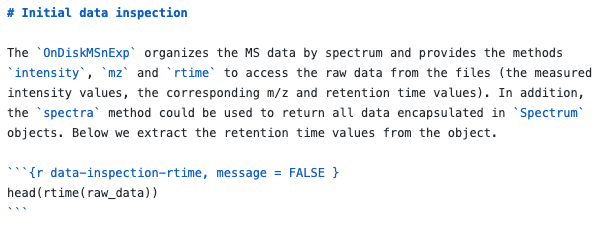
\includegraphics[width=\textwidth]{figures/plaintext_vignette_example} \caption[An example of a the plain text used to write a knitted document]{An example of a the plain text used to write a knitted document. This shows a section of the plain text used to write the online vignette for the `xcms` package from Bioconductor. The full plain text file used for the vignette can be viewed on GitHub [here](https://github.com/sneumann/xcms/blob/master/vignettes/xcms.Rmd).}\label{fig:xcmsexampleplain}
\end{figure}

There are a few things to keep in mind when writing plain text. First, you
should always use a text editor rather than a word processor when you are
writing a document in plain text. Text editors can include software programs
like Notepad on Microsoft operating systems and TextEdit on Mac operating
systems. You can also use a more advanced text editor, like vi/vim or emacs.
Rstudio can also serve as a text editor, and if you are doing other work in
Rstudio, this is often the most obvious option as a text editor to use to write
knitted documents.

You must use a text editor to write plain text for knitted documents for the
same reasons that you must use one to write code scripts. Word processors often
introduce formatting that is saved through underlying code rather than clearly
evident on the document that you see as you type. This hidden formatting can
complicate the written text. Conversely, text written in a text editor will not
introduce such hard-to-see formatting. Word processing programs also tend to
automatically convert some symbols into slightly fancier versions of the symbol.
For example, they may change a basic quotation symbol into one with shaping,
depending on whether the mark comes at the beginning or end of a quotation. This
subtle change in formatting can cause issues in both the code and the formatting
specifications that you include in a knitted document.

Further, when are writing plain text, typically you should only use characters
from the American Standard Code for Information Interchange, or ASCII. This is a
character set from early in computing that includes 128 characters. Such a small
character set enforces simplicity: this character set mostly includes what you
can see on your keyboard, like the digits 0 to 9, the lowercase and uppercase
alphabet, some symbols, including punctuation symbols like the exclamation point
and quotation marks, some mathematical symbols like plus, minus, and division,
and some control codes, including ones for a new line, a tab, and even ringing a
bell. The full set of characters included in ASCII can be found in a number of
sources including a very thorough Wikipedia page on this character set (\url{https://en.wikipedia.org/wiki/ASCII}).

Because the character set available for plain text files is so small, you will
find that it becomes important to leverage the limited characters that are
available. One example is \textbf{white space}. White space can be created in ASCII
with both the space character and with the new line command. It is an important
component that can be used to make plain text files clear for humans to read. As
we begin discussing the convention for markdown languages, we will find that
white space is often used to help specify formatting as well.

The second component of how knitted documents work is that each knitted document
will have a special section at its start called the \textbf{preamble}. This preamble
will give some overall directions regarding the document, like its title and
authors and the format to which is should be rendered. Knitted documents are
created using a \textbf{markup language} to specify formatting for the document, and
there are a number of different markup languages including HTML, LaTeX, and
Markdown. The specifications for the document's preamble will depend on the
markup language being used.

In Rmarkdown, we will be focusing on Markdown, for which the preamble is
specified using something called YAML (short for YAML Ain't Markup Language).
Here is an example of the YAML for a sample pre-processing protocol created
using RMarkdown:

\begin{verbatim}
  ---
  title: "Preprocessing Protocol for LC-MS Data"
  author: "Jane Doe"
  date: "1/25/2021"
  output: pdf_document
  ---
\end{verbatim}

This YAML preamble specifies information about the document with \textbf{keys} and
\textbf{values}. For example, the title is specified using the YAML key \texttt{title},
followed by a colon and a space, and then the desired value for that
component of the document, \texttt{"Preprocessing\ Protocol\ for\ LC-MS\ Data"}.
Similarly, the author is specified with the \texttt{author} key and the desired
value for that component, and the date with the \texttt{date} key and associated
component.

Different keys can take different types of values in the YAML
(this is similar to how different parameters in a function can take different values). For example, the keys of \texttt{author}, \texttt{title}, and \texttt{date} all take
a character string with any desired character combination, and the quotation
marks surrounding the values for each of these keys denote those character strings. By contrast, the \texttt{output} key---which specifies the format that
that the knitted document should be rendered to---can only take one of a
few set values, each of which is specified without surrounding
quotation marks (\texttt{pdf\_document} in this case, to render the document
as a PDF report).

The rules for which keys can be included in the preamble will depend on the
markup language being used. Here, we are showing an example in Markdown, but you
can also use other markup languages like LaTeX and HTML, and these will have
their own convention for specifying the preamble. Later in this module, when we
talk more specifically about Rmarkdown, we will give some resources where you
can find more about how to customize the preamble in Rmarkdown specifically. If
you are using a different markup language, there are numerous websites,
cheatsheets, and other resources you can use to find which keywords are
available for the preamble in that markup language, as well as the possible
values those keywords can take.

The next characteristic of knitted documents is that they need to clearly
demarcate where executable code starts and where regular formatted text starts
(in other words, where the executable code section ends). To do this, knitted
documents have two special combination of characters, one that can be used in
the plain text to indicate where executable code starts and and one to indicate
where it ends. For example, Figure \ref{fig:demarcatecode} shows the plain text
that could be used in an Rmarkdown document to write some regular text, then
some executable code, and then indicate the start of more regular text:

\begin{figure}
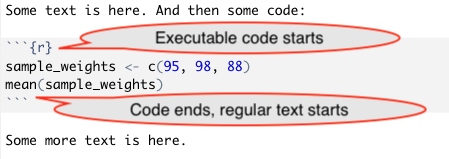
\includegraphics[width=\textwidth]{figures/demarcating_code} \caption[An example of how special combinations of characters are used to demarcate code in an RMarkdown file]{An example of how special combinations of characters are used to demarcate code in an RMarkdown file. The color formatting here is applied automatically by RStudio; all the text in this example is written in plain text.}\label{fig:demarcatecode}
\end{figure}

The combination that indicates the start of executable code will vary depending
on the markup language being. In Rmarkdown, the following combination indicates
the start of executable code:

\texttt{\textasciigrave{}\textasciigrave{}\textasciigrave{}\{r\}}

\noindent while this combination indicates the end of executable code (in other
words the start of regular text):

\texttt{\textasciigrave{}\textasciigrave{}\textasciigrave{}}

In Figure \ref{fig:demarcatecode} and above, we have shown the most basic
version of the markup character combination used to specify the start of
executable code (\texttt{\textasciigrave{}\textasciigrave{}\textasciigrave{}\{r\}}). This character combination can be expanded,
however, to include some specifications for how you want the code in the section
following it to be run, as well as how you want output to be shown. For example,
you could use the following indications to specify that the code should be run,
but the code itself should not be printed in the final document, by specifying
\texttt{echo\ =\ FALSE}, as well as that the created figure should be centered on the
page, by specifying \texttt{fig.align\ =\ "center"}:

\texttt{\textasciigrave{}\textasciigrave{}\textasciigrave{}\{r\ echo\ =\ FALSE,\ fig.align\ =\ "center"\}}

There are numerous options that can be used to specify how the code will be run,
and later when we talk specifically about Rmarkdown, we will point toward
resources that clarify and outline all the possible choices that can be used for
these specifications.

You may have noticed that these markers, which indicate the beginning and end of
executable code, seem like very odd character combination. There is a good
reason for this. By making this character combination unusual, there will be
less of a chance that it shows up in regular text. This way there are fewer
cases where the writer unintentionally indicate the start of a new section of
executable code when trying to write regular text in the knitted document.

The next characteristic of knitted documents is that formatting for the regular
text in the document---that is, everything that is not executable code---is
specified using what is called a \textbf{markup language}. When you were writing in
plain text, you do not have buttons to click on for formatting, for example, to
specify words or phrases that should be in bold or italics, font size, headings,
and so on. Instead you use special characters or character combinations to
specify formatting in the final document. These character combinations are
defined based on the markup language you use. As mentioned earlier, Rmarkdown
uses the Markdown language; other knitted documents can be created using LaTeX
or HTML. As an example of how these special character combinations work, in
Markdown, you place two asterisks around a word or phrase to make it bold. To
write ``\textbf{this}'' in the final document, in other words, you'll write
\texttt{"**this**"} in the plain text in the initial document.

You can start to see how this works by looking at the example of the \texttt{xcms}
vignette shown earlier in Figures \ref{fig:xcmsexample} and
\ref{fig:xcmsexampleplain}. In Figure \ref{fig:xcmsbothversions}, we've
recreated these two parts side-by-side, so they're easier to compare.

\begin{figure*}
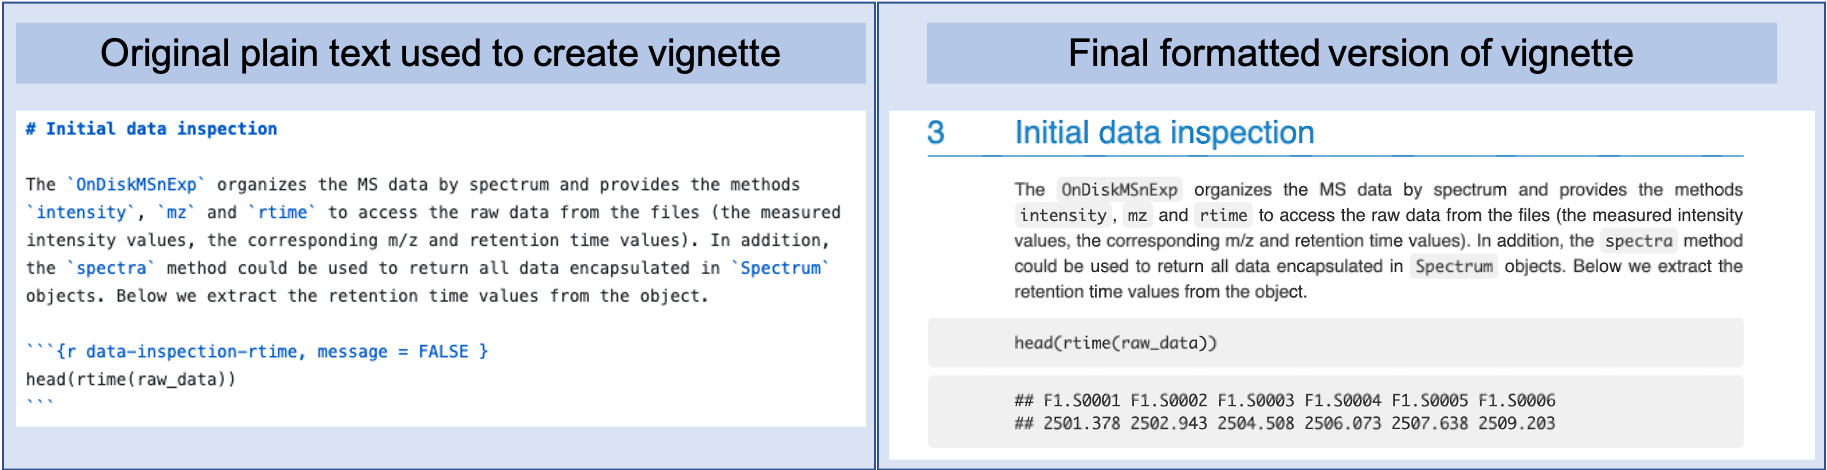
\includegraphics[width=\textwidth]{figures/originalandfinal} \caption[The original plain text for a knitted document and the final output, side by side]{The original plain text for a knitted document and the final output, side by side. These examples are from the `xcms` package vignette, a package available on Bioconductor. The left part of the figure shows the plain text that was written to create the output, which is shown in the left part of the figure. You can see how elements like sections headers and different font styles are indicated in the original plain text through special characters or combinations of charaters, using the Markdown language syntax.}\label{fig:xcmsbothversions}
\end{figure*}

You can look for several formatting elements here. First, the section is headed
``Initial data inspection''. You can that in the original plain text document,
this is marked using a \texttt{\#} to start the line with the text for the header. You
can also see that words or phrases that are formatted in a computer-style font
in the final document---to indicate that they are values from computer code,
rather than regular English words---are surrounded by backticks in the plain
text file.

The process of writing your document in this way can feel a little like the
old-fashioned style of dictating to a secretary. You can imagine yourself
dictating to the computer through the plain text. You have to say not just the
words, but also specify in the plain text the formatting that you want at each
spot. For example, when you get to a word that you want in italics, you must
tell the computer, ``Start italics,'' then say the word, then ``End italics''. You
do this using the special formatting characters that are specified by the markup
language that you use. Later in this module we will point to resources for
discovering all of these formatting specifications for Markdown, the markup
language used by RMarkdown.

The final characteristics of knitted documents is that, to create the final
document, you will render the plain text document. That is the process that will
create an attractive final document. To visualize this, \textbf{rendering} is the
process that takes the document from the plain text format, as shown in the left
of Figure \ref{fig:xcmsbothversions}, to the final format, shown in the right
of that figure.

When you render the document, it will be run through two software programs. The
first will look only for sections with executable code, based on the character
combination that is used to mark these executable code sections. This first
software will execute that code and take any output---including data results,
figures, and tables---and insert those at the relevant spot in the document's
file. Next, these output file from this software run will be run through another
software program. This second program will look for all the formatting
instructions and render the final document in an attractive format. This final
output can be in a number of file formats, depending what you specify in the
preamble, including a PDF document, an HTML file, or a Word document.

You should consider the final document, regardless of the output format, as
read-only. This means that you should never make edits or changes to the final
version of the document. Instead you should make any changes to your initial
plain text file. This is because the rendering process will overwrite any
previous versions of the final document. Therefore any changes that you have
made to your final document will be overwritten anytime you re-render from the
original plain text document.

\hypertarget{quotes}{%
\subsection{Quotes}\label{quotes}}

\begin{quote}
``It's very important to keep a project notebook containing detailed information
about the chronology of your computational work, steps you've taken, information
about why you've made decisions, and of course all pertinent information to
reproduce your work. Some scientists do this in a handwritten notebook, others in
Microsoft Word documents. As with README files, bioinformaticians usually like keeping
project notebooks in simple plain-text because these can be read, searched, and
edited from the command line and across network connections to servers. Plain text
is also a future-proof format: plain-text files written in the 1960s are still
readable today, whereas files from word processors only 10 years old can be
difficult or impossible to open and edit. Additionally, plain text project notebooks can
also be put under version control \ldots{} While plain-text is easy to write in your
text editor, it can be inconvenient for collaborators unfamiliar with the command
line to read. A lightweight markup language called \emph{Markdown} is a plain-text format
that is easy to read and painlessly incorporated into typed notes, and can also be
rendered to HTML or PDF.'' \citep{buffalo2015bioinformatics}
\end{quote}

\begin{quote}
``Markdown originates from the simple formatting conventions used in plain-text
emails. Long before HTML crept into email, emails were embellished with simple
markup for emphasis, lists, and blocks of text. Over time, this became a defacto
plain-text email formatting scheme. This scheme is very intuitive: underscores or
asterisks that flank text indicate emphasis, and lists are simply lines of text
beginning with dashes.'' \citep{buffalo2015bioinformatics}
\end{quote}

\begin{quote}
``Markdown is just plain-text, which means that it's portable and programs to edit
and read it will exist. Anyone who's written notes or papers in old versions of
word processors is likely familiar with the hassle of trying to share or update
out-of-date proprietary formats. For these reasons, Markdown makes for a simple
and elegant notebook format.'' \citep{buffalo2015bioinformatics}
\end{quote}

\begin{quote}
``Information, whether data or computer code, should be organized in such a way that
there is only one copy of each important unit of information.'' \citep{murrell2009introduction}
\end{quote}

\begin{quote}
``A typical encounter with Bioconductor (Box 1) starts with a specific scientific need, for example, differential analysis of gene expression
from an RNA-seq experiment. The user identifies the appropriate
documented workflow, and because the workflow contains functioning code, the user runs a simple command to install the required
packages and replicate the analysis locally. From there, she proceeds
to adapt the workflow to her particular problem. To this end, additional documentation is available in the form of package vignettes
and manual pages.'' \citep{huber2015orchestrating}
\end{quote}

\begin{quote}
``\textbf{Case study: high-throughput sequencing data analysis.} Analysis of
large-scale RNA or DNA sequencing data often begins with aligning reads to a
reference genome, which is followed by interpretation of the alignment patterns.
Alignment is handled by a variety of tools, whose output typically is delivered
as a BAM file. The Bioconductor packages Rsamtools and GenomicAlignments provide
a flexible interface for importing and manipulating the data in a BAM file, for
instance for quality assessment, visualization, event detection and
summarization. The regions of interest in such analyses are genes, transcripts,
enhancers or many other types of sequence intervals that can be identified by
their genomic coordinates. Bioconductor supports representation and analysis of
genomic intervals with a `Ranges' infrastructure that encompasses data
structures, algorithms and utilities including arithmetic functions, set
operations and summarization (Fig. 1). It consists of several packages
including IRanges, GenomicRanges, GenomicAlignments, GenomicFeatures,
VariantAnnotation and rtracklayer. The packages are frequently updated for
functionality, performance and usability. The Ranges infrastructure was designed
to provide tools that are convenient for end users analyzing data while
retaining flexibility to serve as a foundation for the development of more
complex and specialized software. We have formalized the data structures to the
point that they enable interoperability, but we have also made them adaptable to
specific use cases by allowing additional, less formalized userdefined data
components such as application-defined annotation. Workflows can differ vastly
depending on the specific goals of the investigation, but a common pattern is
reduction of the data to a defined set of ranges in terms of quantitative and
qualitative summaries of the alignments at each of the sites. Examples include
detecting coverage peaks or concentrations in chromatin
immunoprecipitation--sequencing, counting the number of cDNA fragments that match
each transcript or exon (RNA-seq) and calling DNA sequence variants (DNA-seq).
Such summaries can be stored in an instance of the class GenomicRanges.''
\citep{huber2015orchestrating}
\end{quote}

\begin{quote}
``Visualization is essential to genomic data analysis. We distinguish among
three main scenarios, each having different requirements. The first is rapid
interactive data exploration in `discovery mode.' The second is the recording,
reporting and discussion of initial results among research collaborators, often
done via web pages with interlinked plots and tool-tips providing interactive
functionality. Scripts are often provided alongside to document what was done.
The third is graphics for scientific publications and presentations that show
essential messages in intuitive and attractive forms. The R environment offers
powerful support for all these flavors of visualization---using either the various
R graphics devices or HTML5-based visualization interfaces that offer more
interactivity---and Bioconductor fully exploits these facilities. Visualization
in practice often requires that users perform computations on the data, for
instance, data transformation and filtering, summarization and dimension
reduction, or fitting of a statistical model. The needed expressivity is not
always easy to achieve in a point-and-click interface but is readily realized in
a high-level programming language. Moreover, many visualizations, such as heat
maps or principal component analysis plots, are linked to mathematical and
statistical models---for which access to a scientific computing library is
needed.'' \citep{huber2015orchestrating}
\end{quote}

\begin{quote}
" It can be surprisingly difficult to retrace the computational steps
performed in a genomics research project. One of the goals of Bioconductor is to
help scientists report their analyses in a way that allows exact recreation by a
third party of all computations that transform the input data into the results,
including figures, tables and numbers. The project's contributions comprise an
emphasis on literate programming vignettes, the BiocStyle and ReportingTools
packages, the assembly of experiment data and annotation packages, and the
archiving and availability of all previously released packages. \ldots{} Full remote
reproducibility remains a challenging problem, in particular for computations
that require large computing resources or access data through infrastructure
that is potentially transient or has restricted access (e.g., the cloud).
Nevertheless, many examples of fully reproducible research reports have been
produced with Bioconductor." \citep{huber2015orchestrating}
\end{quote}

\begin{quote}
``Using Bioconductor requires a willingness to modify and eventually compose
scripts in a high-level computer language, to make informed choices between
different algorithms and software packages, and to learn enough R to do the
unavoidable data wrangling and troubleshooting. Alternative and complementary
tools exist; in particular, users may be ready to trade some loss of
flexibility, automation or functionality for simpler interaction with the
software, such as by running single-purpose tools or using a point-and-click
interface. Workflow and data management systems such as Galaxy and Illumina
BaseSpace provide a way to assemble and deploy easy-touse analysis pipelines
from components from different languages and frameworks. The IPython notebook
provides an attractive interactive workbook environment. Although its origins
are with the Python programming language, it now supports many languages,
including R. In practice, many users will find a combination of platforms most
productive for them.'' \citep{huber2015orchestrating}
\end{quote}

\begin{quote}
``A lab manual is perhaps the best way to inform new lab members of the ins
and outs of the lab and to keep all members updated on protocols and
regulations. What could be included in a lab manual? Anything you do not
want to explain over and over, anything that will make the lab more
functional and that can make life easier for yourself and lab members.'' \citep{leips2010helm}
\end{quote}

\begin{quote}
``Most PIs wish the labs were more organized, but it is not a huge priority,
that is, until the first student leaves and no one can find a particular
cell line in the freezer boxes. Resolutions are made, the crisis passes,
and all goes on as before until the next person leaves. Although it is
probably inevitable that there will be some confusion when a long-time
lab member moves on, an organized lab will not be as affected as an unorganized
one.'' \citep{leips2010helm}
\end{quote}

\begin{quote}
``LaTeX gives you output documents that look great and have consistent
cross-references and citations. Much of your output document is created
automatically and much is done behind the scenes. This gives you extra time to
think about the ideas you want to present and how to communicate those ideas in
an effective way.'' \citep{van2012latex}
\end{quote}

\begin{quote}
``LaTeX provides state-of-the-art typesetting'' \citep{van2012latex}
\end{quote}

\begin{quote}
``Many conferences and publishers accept LaTeX. In addition they provide
classes and packages that guarantee documents conforming to the required
formatting guidelines.'' \citep{van2012latex}
\end{quote}

\begin{quote}
``LaTeX automatically numbers your chapters, sections, figures, and so on.''
\citep{van2012latex}
\end{quote}

\begin{quote}
``LaTeX has excellent bibliography support. It supports consistent citations
and an automatically generated bibliography with a consistent look and
feel. The style of citations and the organisation of the bibliography
is configurable.'' \citep{van2012latex}
\end{quote}

\begin{quote}
``LaTeX is \emph{very} stable, free, and available on many platforms.''
\citep{van2012latex}
\end{quote}

\begin{quote}
``LaTeX was written by Leslie Lamport as an extension of Donald Knuth's
TeX program. It consists of a Turing-complete procedural markup language
and a typesetting processor. The combination of the two lets you control
both the visual presentation \emph{as well as} the content of your documents.''
\citep{van2012latex}
\end{quote}

\begin{quote}
``Roughly speaking LaTeX is built on top of TeX. This adds extra functionality
to TeX and makes writing your documents much easier.'' \citep{van2012latex}
\end{quote}

\begin{quote}
``To create a perfect output file and have consistent cross-references
and citations, latex also writes information to and reads information from
\emph{auxiliary} files. Auxiliary files contain information about page numbers of
chapters, sections, tables, figures, and so on. Some auxiliary files are
generated by latex itself (e.g., aux files). Others are generated by
external programs such as bibtex, which is a program that generates information
for the bibliography. When an auxiliary file changes then LaTeX may be out
of sync. You should rerun latex when this happens.'' \citep{van2012latex}
\end{quote}

\begin{quote}
``LaTeX is a markup language and document preparation system. It forces you
to focus on the content and \emph{not} on the presentation. In a LaTeX program
you write the content of your document, you use commands to provide markup
and automate tasks, and you import libraries.'' \citep{van2012latex}
\end{quote}

\begin{quote}
``The main purpose of {[}LaTeX{]} commands is to provide markup. For example,
to specify the author of the document you write \texttt{\textbackslash{}author\{\textless{}author\ name\textgreater{}\}}.
The real strength of LaTeX is that it also is a Turing-complete programming
language, which lets you define your own commands. These commands let you do
real programming and give you ultimate control over the content and the
final visual presentation. You can reuse your commands by putting them in
a library.'' \citep{van2012latex}
\end{quote}

\begin{quote}
``The paragraph is one of the most important basic building blocks of your
document. The paragraph formation rules depend on how latex treats spaces,
empty lines, and comments. Roughly, the rules are as follows. In its default
model, latex treats a sequence of one or more spaces as a single space. The
end of the line is the same as a space. However: An empty line acts
as an end-of-paragraph specifier\ldots{}'' \citep{van2012latex}
\end{quote}

\hypertarget{discussion-questions-6}{%
\subsection{Discussion questions}\label{discussion-questions-6}}

\hypertarget{module19}{%
\section{RMarkdown for creating reproducible data pre-processing protocols}\label{module19}}

The R extension package RMarkdown can be used to create documents that combine
code and text in a `knitted' document, and it has become a popular tool for
improving the computational reproducibility and efficiency of the data analysis
stage of research. This tool can also be used earlier in the research process,
however, to improve reproducibility of pre-processing steps. In this module, we
will provide detailed instructions on how to use RMarkdown in RStudio to create
documents that combine code and text. We will show how an RMarkdown document
describing a data pre-processing protocol can be used to efficiently apply the
same data pre-processing steps to different sets of raw data.

\textbf{Objectives.} After this module, the trainee will be able to:

\begin{itemize}
\tightlist
\item
  Define RMarkdown and the documents it can create
\item
  Explain how RMarkdown can be used to improve the reproducibility of research
  projects at the data pre-processing phase
\item
  Create a document in RStudio using RMarkdown
\item
  Apply it to several different datasets with the same format
\end{itemize}

\hypertarget{creating-knitted-documents-in-r}{%
\subsection{Creating knitted documents in R}\label{creating-knitted-documents-in-r}}

In the last module, we described what knitted documents are, as well as the
advantages of using knitted documents to create data pre-processing protocols
for common pre-processing tasks in your research group. In this module, we will
go into more detail about how you can create these documents using R and
RStudio, and in the next module we will walk through an example data
pre-processing protocol created using this method.

R has a special format for creating knitted documents called \textbf{Rmarkdown}.
Later in this module, we will provide details on creating these documents, but
first, we will provide some details of some of the specific conventions used in
this type of knitted documents. As with other knitted documents, Rmarkdown
documents are originally written in plain text. In the previous module, we
discussed how knitted documents will use a markup language within the plain text
for formatting; for RMarkdown files, the markup language used is Markdown. Since
the laguage is Markdown, the preamble for each document uses YAML. We described
in the previous module how knitted documents include executable code, along with
the formatted text. By default, executable code for RMarkdown files will be in
R, but there are also options to include executable code in the document in a
number of other programming languages.

\hypertarget{creating-and-exploring-an-rmarkdown-file}{%
\subsection{Creating and exploring an Rmarkdown file}\label{creating-and-exploring-an-rmarkdown-file}}

\textbf{Creating a new Rmarkdown file and exploring the template.}

First, we will explain how you can create a new Rmarkdown document using
RStudio. Like other plain text documents, an Rmarkdown file should be edited
using a text editor, rather than a word processor like Word or Google Docs. It
is easiest to use the Rstudio IDE as the text editor when creating and editing
an R markdown document, as this IDE has incorporated some helpful functionality
for working with plain text documents for Rmarkdown. The RStudio IDE can be
downloaded and installed as a free software, as long as you use the personal
version (RStudio creates higher-powered versions for corporate use). Since
RStudio is free and has many helpful tools for working with Rmarkdown, we will
focus on using this interface in our advice in this module.

In RStudio, you can create a number of types of new files through the
``File'' menu. To create a new R markdown file, choose ``New File'' and then choose
``Rmarkdown'' from the choices in that menu. Figure \ref{fig:rmarkdownnewfile}
shows an example of what this menu option looks like.

\begin{figure}
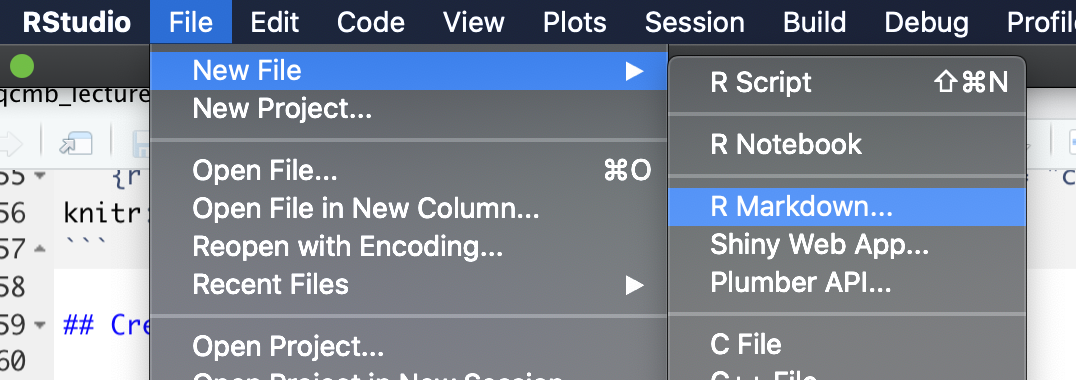
\includegraphics[width=\textwidth]{figures/rmarkdown_newfile} \caption[RStudio pull-down menus to help you navigate to open a new Rmarkdown file]{RStudio pull-down menus to help you navigate to open a new Rmarkdown file.}\label{fig:rmarkdownnewfile}
\end{figure}

This will open a window with some options you can specify some of the overall
information about the document (Figure \ref{fig:rmarkdownchoices}), including
the title and the author, and you can specify the output format that you would
like. Possible output formats include HTML, Word, and PDF. You should be able to
use the HTML and Word output formats without any additional software. If you
would like to use the PDF output, you will need to install one other piece of
software: Miktex for Windows, MacTex for Mac, or TeX Live for Linux. These are
all pieces of software with an underlying TeX engine and all are open-source and
free.

\begin{figure}
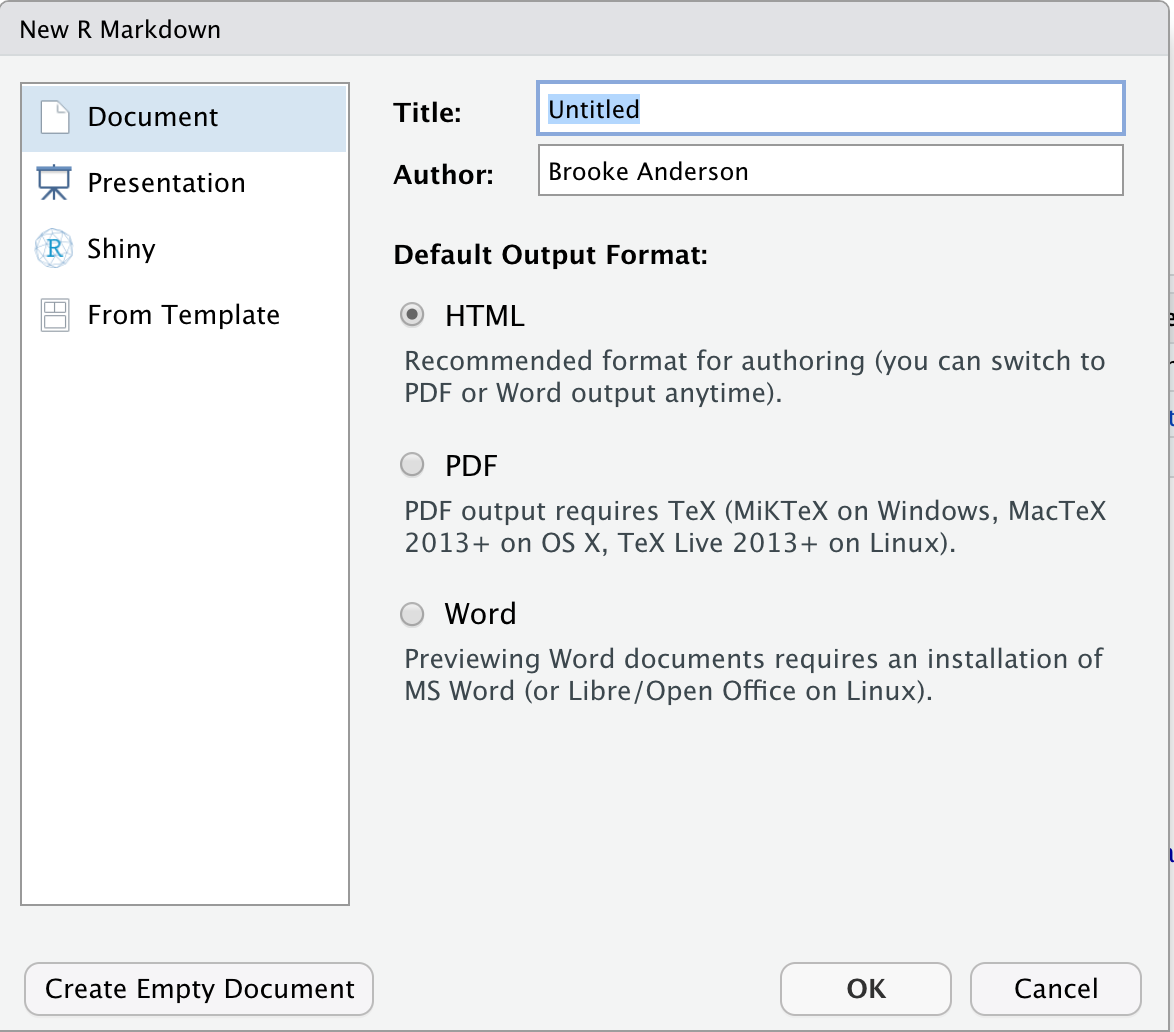
\includegraphics[width=\textwidth]{figures/rmarkdown_choices} \caption[Options available when you create a new Rmarkdown file in RStudio]{Options available when you create a new Rmarkdown file in RStudio. You can specify information that will go into the document's preamble, including the title and authors and the format that the document will be output to (HTML, Word, or PDF).}\label{fig:rmarkdownchoices}
\end{figure}

Once you have selected the options in this menu you can choose the ``Okay'' button
(Figure \ref{fig:rmarkdownchoices}). This will open a new document. This
document, however, won't be blank. Instead it will include an example document
written in Rmarkdown (Figure \ref{fig:rmarkdowntemplate}). This example
document helps you navigate how the Rmarkdown process works, by letting you test
out a sample document. It also gives you a starting point---once you understand
how the example document works, you can edit it and change it to convert it
into the document you would like to create.

\begin{figure}
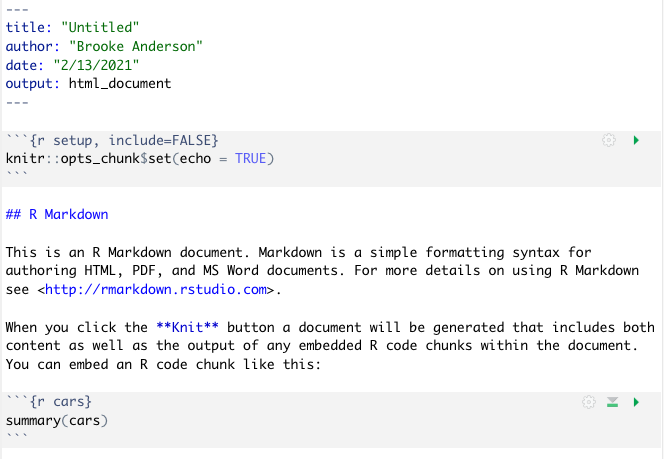
\includegraphics[width=\textwidth]{figures/rmarkdown_template} \caption[Example of the template Rmarkdown document that you will see when you create a new Rmarkdown file in RStudio]{Example of the template Rmarkdown document that you will see when you create a new Rmarkdown file in RStudio. You can explore this template and try rendering (knitting) it. Once you are familiar with how this example works, you can edit the text and code to adapt it for your own document.}\label{fig:rmarkdowntemplate}
\end{figure}

If you have not used Rmarkdown before, it is very helpful to try knitting this
example document before making changes, to explore how pieces in the document
align with elements in the rendered output document. Once you are
familiar with the line-up between elements in this file in the output document,
you delete parts of the example file and insert your own text and code.

We will walk you through exploring this example document, as well as aligning it
with the formatted output document (Figure \ref{fig:rmarkdownoriginalfinal}).
First, to render this or any Rmarkdown document, if you are in RStudio you can
use the ``Knit'' button at the top of the file, as shown in Figure
\ref{fig:rmarkdowntemplate2}. When you click on this button, it will render the
entire document to the output format you've selected (HTML, PDF, or Word). This
rendering process will both run the executable code and apply all formatting.
The final output (Figure \ref{fig:rmarkdownoriginalfinal}, right) will pop up
in a new window. As you start with Rmarkdown, it is useful to look at this
output to see how it compares with the plain text Rmarkdown file (Figure
\ref{fig:rmarkdownoriginalfinal}, left).

\begin{figure*}
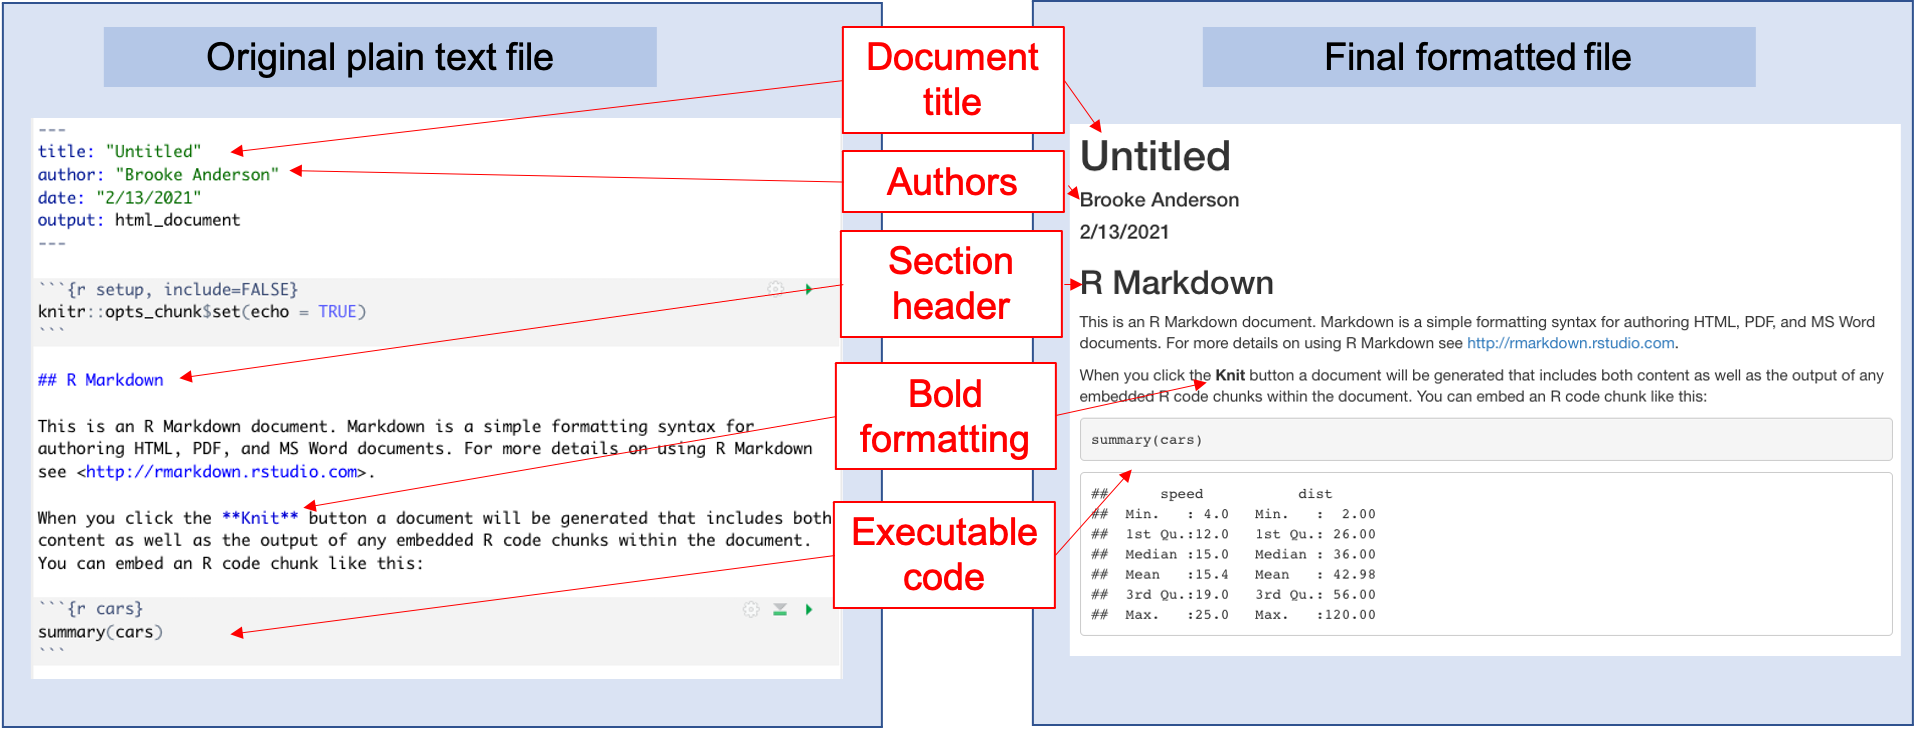
\includegraphics[width=\textwidth]{figures/rmarkdownoriginalfinal} \caption[Example of the template Rmarkdown document that you will see when you create a new Rmarkdown file in RStudio]{Example of the template Rmarkdown document that you will see when you create a new Rmarkdown file in RStudio. You can explore this template and try rendering (knitting) it. Once you are familiar with how this example works, you can edit the text and code to adapt it for your own document.}\label{fig:rmarkdownoriginalfinal}
\end{figure*}

\begin{figure}
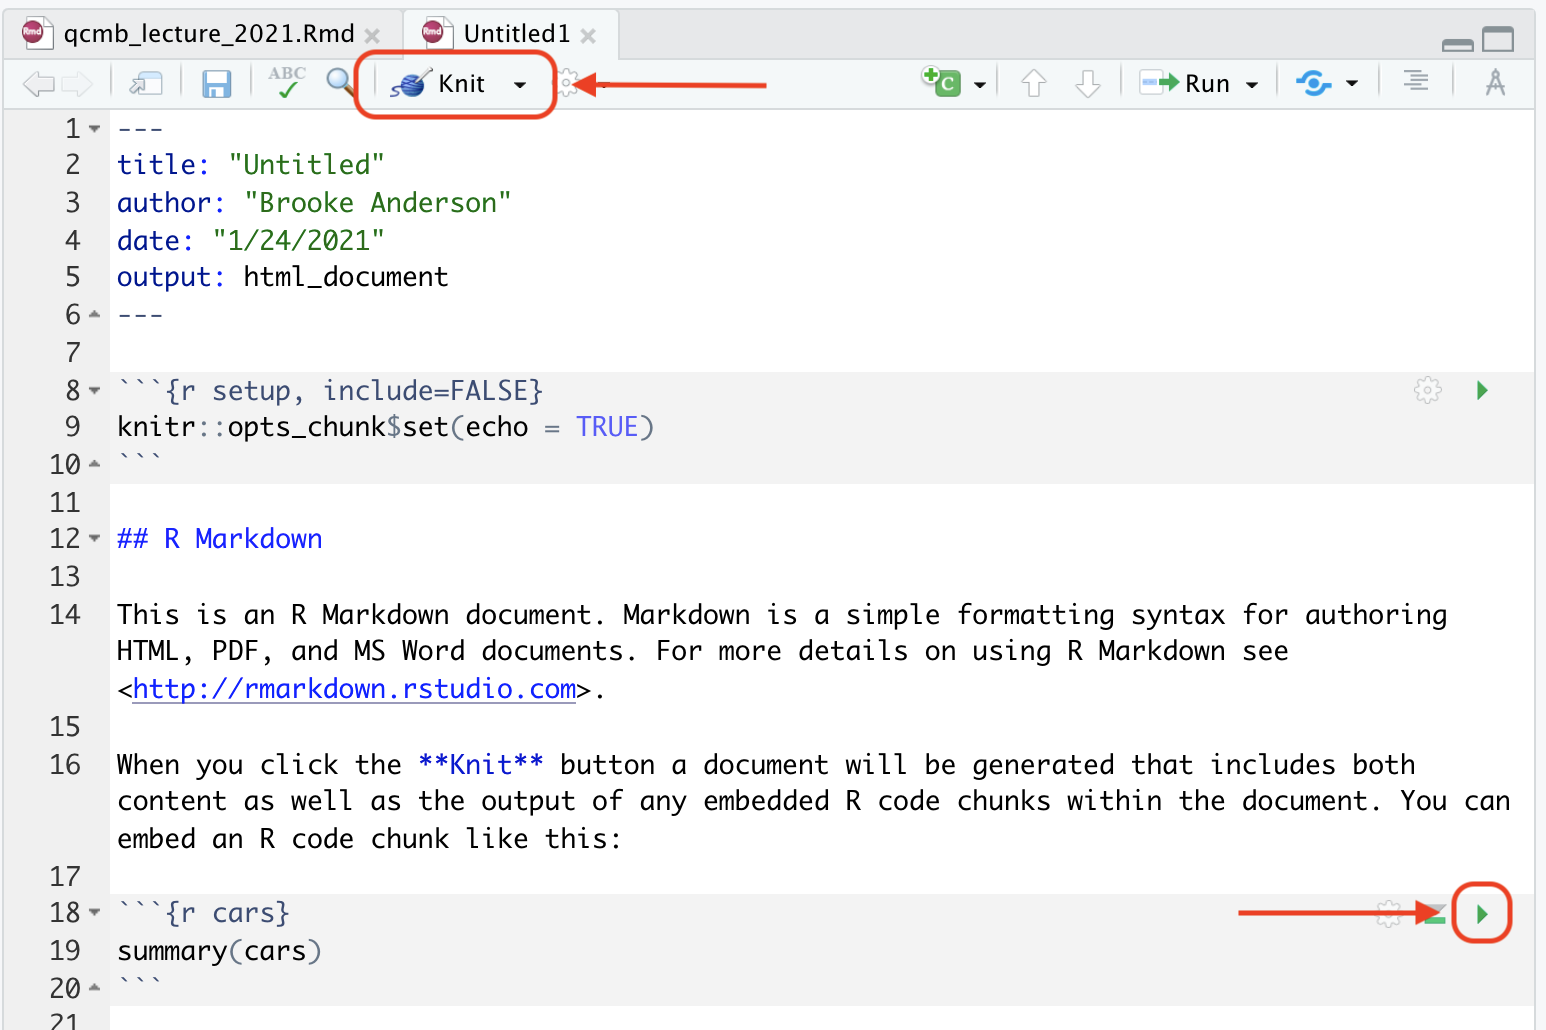
\includegraphics[width=\textwidth]{figures/rmarkdown_template2} \caption[Example of the template Rmarkdown document, highlighting buttons in RStudio that you can use to facilitate working with the document]{Example of the template Rmarkdown document, highlighting buttons in RStudio that you can use to facilitate working with the document. The 'knit' button, highlighted at the top of the figure, will render the entire document. The green arrow, highlighted lower in the figure within a code chunk, can be used to run the code in that specific code chunk.}\label{fig:rmarkdowntemplate2}
\end{figure}

You will also notice, after you first render the document, that your working
directory has a new file with this output document. For example, if you are
working to create an HTML document using an Rmarkdown file called
``my\_report.Rmd'', once you knit your Rmarkdown file, you will notice a new file
in your working directory called ``my\_report.html''. This new file is your output
file, the one that you would share with colleagues as a report. You should
consider this output document to be read only---in other words, you can read and
share this document, but you should not make any changes directly to this
document, since they will be overwritten anytime you re-render the original
Rmarkdown document.

Next, let's compare the example Rmarkdown document (the one that is given when
you first open an Rmarkdown file in RStudio) with the output file that is
created when you render this example document (Figure
\ref{fig:rmarkdownoriginalfinal}). If you look at the output document (Figure
\ref{fig:rmarkdownoriginalfinal}, right), you can notice how different elements
align with pieces in the original Rmarkdown file (Figure
\ref{fig:rmarkdownoriginalfinal}). For example, the output document includes a
header with the text ``R Markdown''. This second-level header is created by the
Markdown notation in the original file of:

\begin{verbatim}
## R Markdown
\end{verbatim}

This header is formatted in a larger font than other text, and on a separate
line---the exact formatting is specified within the style file for the Rmarkdown
document, and will be applied to all second-level headers in the document. You
can also see formatting specified through things like bold font for the word
``Knit'', through the Markdown syntax \texttt{**Knit**}, and a clickable link specified
through the syntax \texttt{\textless{}http://rmarkdown.rstudio.com\textgreater{}}. At the beginning of the
original document, you can see how elements like the title, author, date, and
output format are specified in the YAML. Finally, you can see that special
character combinations demarcate sections of executable code.

\textbf{Formatting text with Markdown.}

For the main text in an Rmarkdown document, all formatting is done using
Markdown as the markup language. Markdown is a popular markup language, in part
because it is a good bit simpler than other markup languages like HTML or LaTeX.
This simplicity means that it is not quite as expressive as other markup
languages. However, Markdown provides adequate formatting for 90\% of the
formatting you will typically want to do for a research report or
pre-processeing protocol, and by staying simpler, it is much easier to learn the
Markdown syntax quickly compared to other markup languages.

As with other markup languages, Markdown uses special characters or combinations of characters to indicate formatting within the plain text of the original document. When the document is rendered, these markings are used by the software to create the formatting that you have specified in the final output document. Some example formatting symbols and conventions for Markdown include:

\begin{itemize}
\tightlist
\item
  to format a word or phrase in bold, surround it with two asterisks (\texttt{**})
\item
  to format a word or phrase in italics, surround it with one asterisk (\texttt{*})
\item
  to create a first-level header, put the header text on its own line, starting the line with \texttt{\#}
\item
  to create a second-level header, put the header text on its own line, starting the line with \texttt{\#\#}
\item
  separate paragraphs with empty lines
\item
  use hyphens to create bulleted lists
\end{itemize}

One thing to keep in mind when using Markdown, in terms of formatting, is that
white space can be very important in specifying the formatting. For example when
you specify a new paragraph, you must leave a blank line from your previous
text. Similarly when you use a hash (\texttt{\#}) to indicate a header, you must leave a
blank space after the hash before the word or phrase that you want to be used in
that header. To create a section header, you would write:

\begin{verbatim}
# Initial Data Inspection
\end{verbatim}

Meanwhile this:

\begin{verbatim}
#Initial Data Inspection
\end{verbatim}

Would render to:

\#Initial Data Inspection

Similarly, white space is needed to separate paragraphs. For example, this would create two paragraphs:

\begin{verbatim}
This is a first paragraph. 

This is a second.
\end{verbatim}

Meanwhile this would create one:

\begin{verbatim}
This is a first paragraph.
This is still part of the first paragraph.
\end{verbatim}

The syntax of Markdown is fairly simple and can be learned quickly. For more
details on this syntax, you can refer to the Rmarkdown reference guide at
\url{https://rstudio.com/wp-content/uploads/2015/03/rmarkdown-reference.pdf}. The
basic formatting rules for Markdown are also covered any number of more
extensive resources for Rmarkdown that we will point you to later in this
module.

\textbf{Creating a preamble with YAML.}

In the previous module, we explained how knitted documents include a
preamble to specify some metadata about the document, including elements
like the title, authors, and output format. In R, this preamble is
created using YAML. In this subsection, we provide some more details
on using this YAML section in Rmarkdown documents.

When you initially create an Rmarkdown document, you select the output format
for it (e.g., pdf, Word, HTML). You can change this output selection once you've
created the document, however, by making a change in a special section at the
top of the RMarkdown document called the ``YAML''. The YAML is a special section
at the top of an RMarkdown document (the original, plain text file, not the
rendered version). It is set off from the rest of the document using a special
combination of characters, using a process very similar to how executable code
is set off from other text with a special set of characters so it can be easily
identified by the software program that renders the document. For the YAML, this
combination of characters is three hyphens (\texttt{-\/-\/-}) on a line by themselves to
start the YAML section and then another three on a line by themselves to end it.
Here is an example of what the YAML might look like at the top of an RMarkdown
document:

\begin{verbatim}
---
title: "Laboratory report for example project"
author: "Brooke Anderson"
date: "1/12/2020"
output: word_document
---
\end{verbatim}

Within the YAML itself, you can specify different options for your document.
You can change simple things like the title, author, and date, but you can
also change more complex things, including how the output document is rendered.
For each thing that you want to specify, you specify it with a special
keyword for that option and then a valid choice for that keyword. The idea
is very similar to setting parameter values in a function call in R. For
example, the \texttt{title:} keyword is a valid one in RMarkdown YAML. It allows you
to set the words that will be printed in the title space, using title formatting,
in your output document. It can take any string of characters, so you can put in
any text for the title that you'd like, as long as you surround it with quotation
marks. The \texttt{author:} and \texttt{date:} keywords work in similar ways. The \texttt{output:}
keyword allows you to specify the output that the document should be rendered to.
In this case, the keyword can only take one of a few set values, including
\texttt{word\_document} to output a Word document, \texttt{pdf\_document} to output a pdf
document (see later in this section for some more set-up required to make that
work), and \texttt{html\_document} to output an HTML document.

As you start using RMarkdown, you will be able to do a lot without messing with
the YAML much. In fact, you can get a long way without ever changing the values
in the YAML from the default values they are given when you first create an
RMarkdown document. As you become more familiar with R, you may want to learn
more about how the YAML works and how you can use it to customize your
document---it turns out that quite a lot can be set in the YAML to do very
interesting customizations in your final rendered document. The book \emph{R
Markdown: The Definitive Guide} {[}ref{]}, which is available free online, has
sections discussing YAML choices for both HTML and pdf output, at
\url{https://bookdown.org/yihui/rmarkdown/html-document.html} and
\url{https://bookdown.org/yihui/rmarkdown/pdf-document.html}, respectively. There is
also a talk that Yihui Xie, the creator of RMarkdown, gave on this topic at a
past RStudio conference, available at
\url{https://rstudio.com/resources/rstudioconf-2017/customizing-extending-r-markdown/}.

\textbf{Executable code in Rmarkdown files.}

In the previous module, we described how knitted documents use special markers
to indicate where sections of executable code start and stop. In RMarkdown,
the markers you will use to indicate executable code look like this:

\begin{verbatim}
```r{}
my_object <- c(1, 2, 3)
```
\end{verbatim}

The first part of this marker (\texttt{\textasciigrave{}\textasciigrave{}\textasciigrave{}\{r\}}) indicates that a section of
code is starting. Then end part (\texttt{\textasciigrave{}\textasciigrave{}\textasciigrave{}}) indicates that the file is
moving back to regular Markdown. In the first marker, you can use the simplest
form (\texttt{\textasciigrave{}\textasciigrave{}\textasciigrave{}\{r\}}) to indicate the start of the code. However, you can also
include options to customize actions when the code in that section is executed.
There are many options that you can set for each code chunk. These options will
specify how the code in that section of executable code will be run and how the
output from running the code will be presented. These specifications are called
\textbf{chunk options}, and you specify them in the special character combination
where you mark the start of executable code. For example, you can specify that
the code should be printed in the document, but not executed, by setting the
\texttt{eval} parameter to \texttt{FALSE} with \texttt{\textasciigrave{}\textasciigrave{}\textasciigrave{}\{r\ eval\ =\ FALSE\}} as the marker to
start the code section.

The chunk options also include \texttt{echo}, which can be used to specify whether to
print the code in that code chunk when the document is rendered. For some
documents, it is useful to print out the code that is executed, where for other
documents you may not want that printed. For example, for a pre-processing
protocol, you are aiming to show yourself and others how the pre-processing was
done. In this case, it is very helpful to print out all of the code, so that
future researchers who read that protocol can clearly see each step. By
contrast, if you are using Rmarkdown to create a report or an article that is
focused on the results of your analysis, it may make more sense to instead hide
the code in the final document.

As part of the code options, you can also specify whether messages and warnings
created when running the code should be included in the document output, and
there are number of code chunk options that specify how tables and figures
rendered by the code should be shown. For more details on the possible options
that can be specified for how code is evaluated within an executable chunk of
code, you refer to the Rmarkdown cheat sheet available at
\url{https://rstudio.com/wp-content/uploads/2015/02/rmarkdown-cheatsheet.pdf}

RStudio has some functionality that is useful when you are working with code in
Rmarkdown documents. Within each code chuck are some buttons that can be used to
test out the code in that chunk of executable code. One is the green right arrow
key to the right at the top of the code chunk, highlighted in Figure
\ref{fig:rmarkdowntemplate2}. This button will run all of the code in that
chunk and show you the output in an output field that will open directly below
the code chunk. This functionality allows you to explore the code in your
document as you build it, rather than waiting until you are ready to render the
entire document. The button directly to the left of that button, which looks
like an upward-pointing arrow over a rectangle, will execute all code that comes
before this chunk in the document. This can be very helpful in making sure that
you have set up your environment to run this particular chunk of code.

\hypertarget{more-advanced-rmarkdown-functionality}{%
\subsection{More advanced Rmarkdown functionality}\label{more-advanced-rmarkdown-functionality}}

The details and resources that we have covered so far focus on the basics of
Rmarkdown. You can get a lot done just with these basics. However, the Rmarkdown
system is very rich and allows complex functionality beyond these basics. In
this subsection, we will highlight just a few of the ways Rmarkdown can be used
in a more advanced way. Since this topic is so broad, we will focus on elements
that we have found to be particularly useful for biomedical researchers as they
become more advanced Rmarkdown users. For the most part, we will not go into
extensive detail about how to use these more advanced features in this module,
but instead point to resources where you can learn more as you are ready. If you
are just learning Rmarkdown, at this point it will be helpful to just know that
some of these advanced features are available, so you can come back and explore
them when you become familiar with the basics. However, we will provide more
details for two elements that we find particularly useful in creating data
pre-processing protocols: including bibliographical references and including
mathematical equations. In the next module, we walk through an example of using
RMarkdown, and in this example we show how you can use these two more advanced
features when creating a pre-processing protocol.

\textbf{Including bibliographical references.}

You can use Rmarkdown, in combination with something called BibTeX, as a
referencing system. This allows you to include bibliographical references in the
documents that you create, and Rmarkdown will handle the creation of the
references section and the numbering of the documents within your text.

To include references in RMarkdown documents, you can use something called
\textbf{BibTeX}. This has three components:

\begin{enumerate}
\def\labelenumi{\arabic{enumi}.}
\tightlist
\item
  Create a plain text file with listings for each of
  your references (\textbf{BibTeX file}). Save it with the
  extension \texttt{.bib}.
\item
  In your RMarkdown document, include the filepath
  to this BibTeX file.
\item
  In the text of the RMarkdown file, include a key and special character
  combination anytime you want to reference a paper.
\end{enumerate}

Once you have a BibTeX file, you will include its
path in the YAML:

\begin{verbatim}
  ---
  title: "Reproducible Research with R"
  author: "Brooke Anderson"
  date: "1/25/2021"
  output: beamer_presentation
  bibliography: mybibliography.bib
  ---
\end{verbatim}

It is easiest if you save the BibTeX file in the same directory
as the RMarkdown document.

You can add references in the text using a key for each paper
within special characters (\texttt{{[}@paper1,\ @paper2{]}}).

For example, you would write:

\begin{verbatim}
This technique follows earlier work [@fox2020, 
@anderson2019].
\end{verbatim}

To create:

\begin{quote}
``This technique follows earlier work (Fox et al.~2020, Anderson et al.~2019)."
\end{quote}

With full paper details included at the end of the document.

Put all the bibliographical details in the BibTeX file:

You will have a file named something like \texttt{mybibliography.bib}
with entries for each paper like this:

\begin{verbatim}
@article{fox2020,
  title={Cyto-feature engineering: A pipeline for flow cytometry 
    analysis to uncover immune populations and associations with 
    disease},
  author={Fox, Amy and Dutt, Taru S and Karger, Burton and Rojas, 
    Mauricio and Obreg{\'o}n-Henao, Andr{\'e}s and 
    Anderson, G Brooke and Henao-Tamayo, Marcela},
  journal={Scientific Reports},
  volume={10},
  number={1},
  pages={1--12},
  year={2020}
}
\end{verbatim}

You can get these details from Google Scholar:

\begin{figure*}
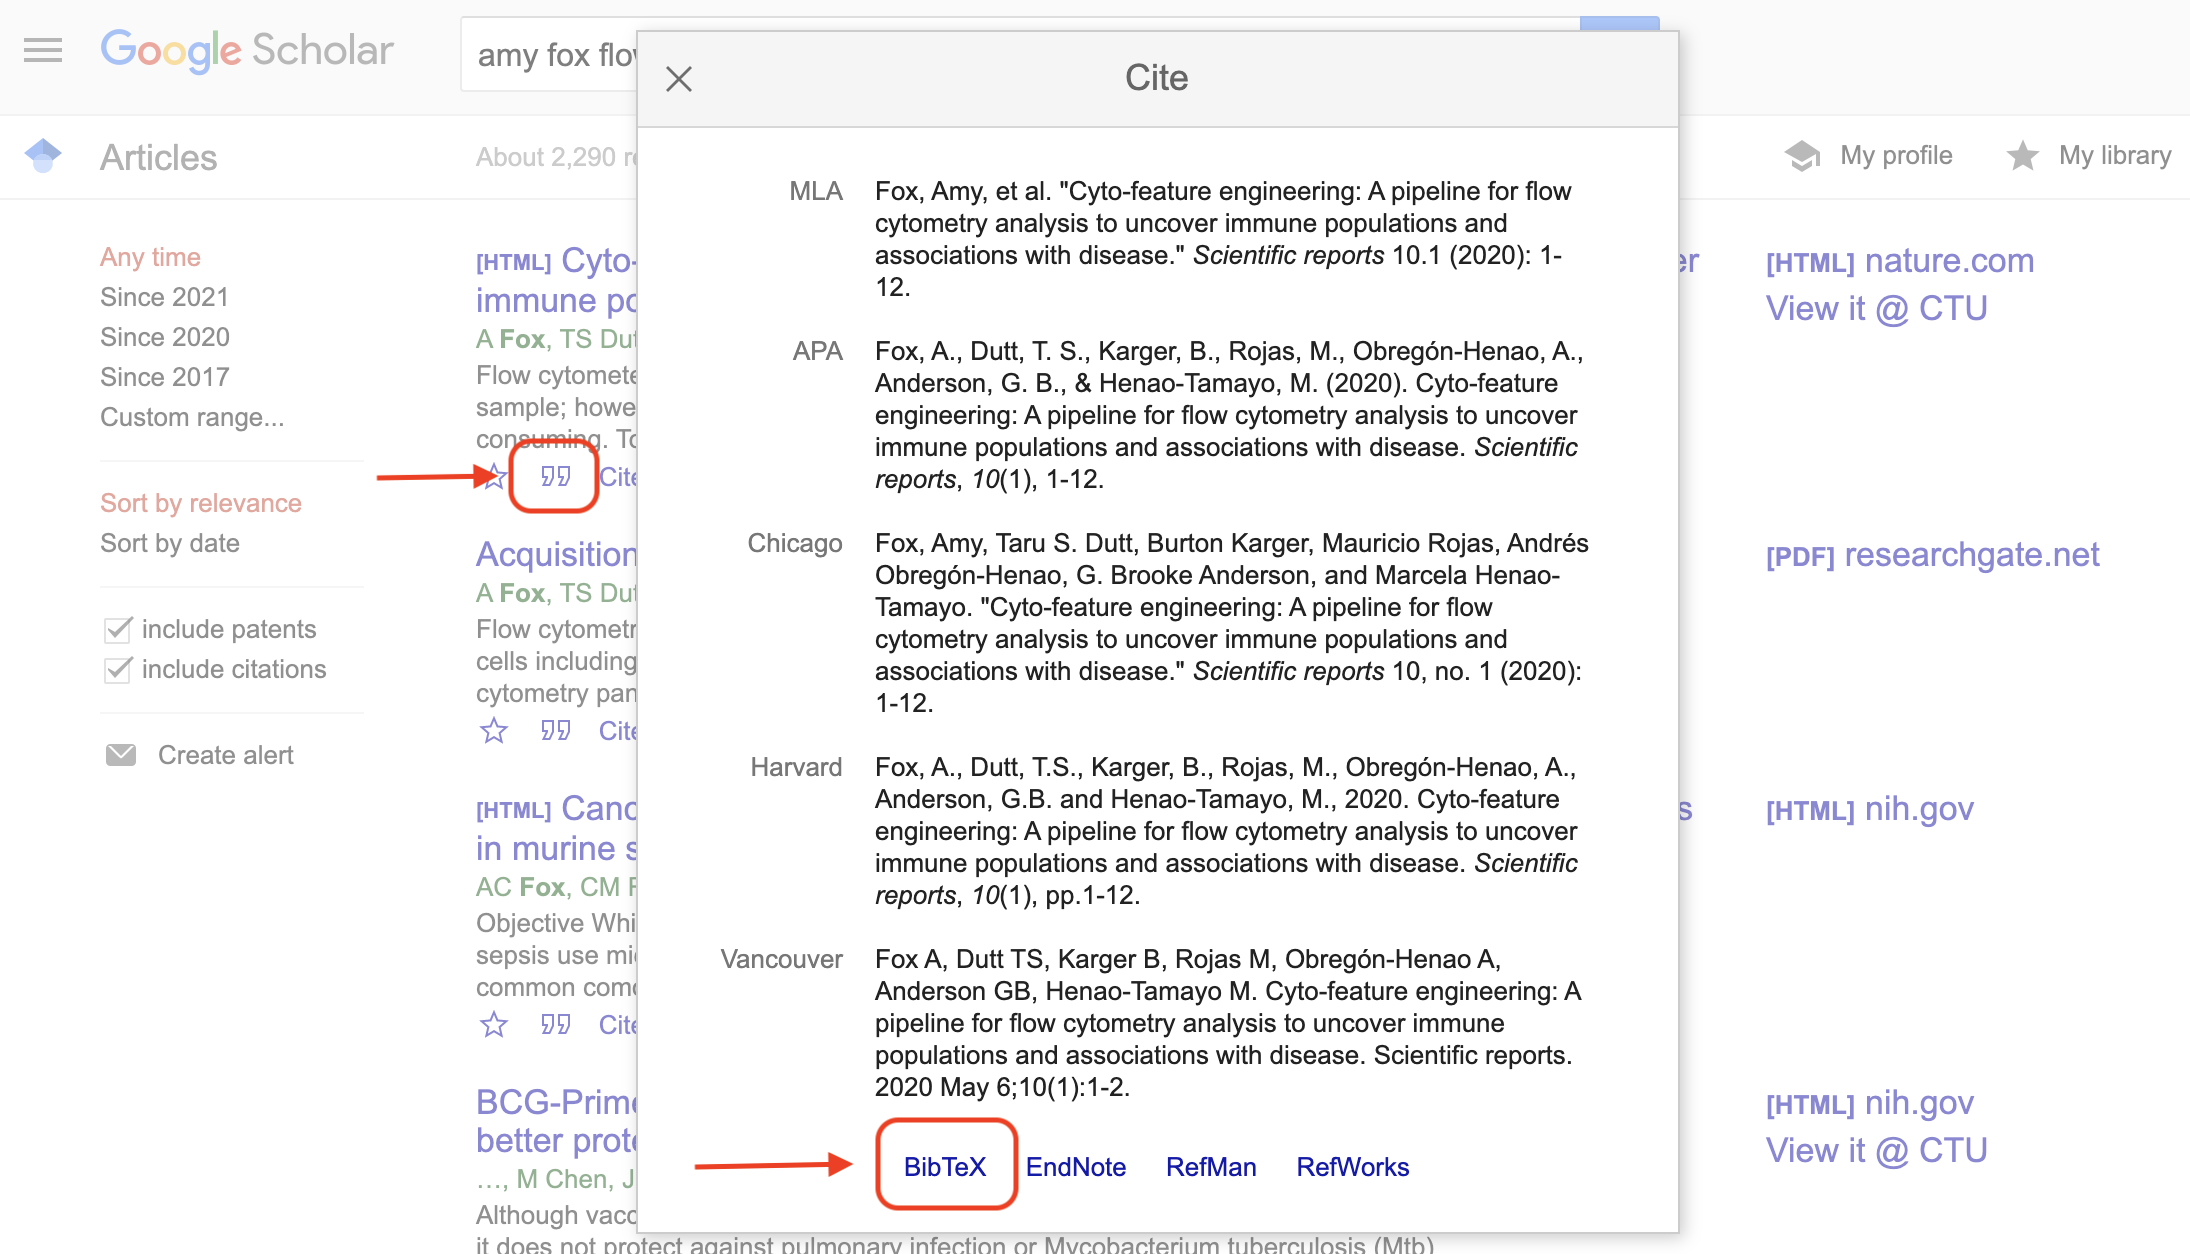
\includegraphics[width=\textwidth]{figures/google_scholar} \caption[Example of using Google Scholar to get bibliographical information for a BibTeX file]{Example of using Google Scholar to get bibliographical information for a BibTeX file. When you look up an article on Google Scholar, there is an option (the quotation mark icon under the article listing) to open a pop-up window with bibliographical information. At the bottom of this pop-up box, you can click on 'BibTeX' to get a plain text version of the BibTeX entry for the article. You can copy and paste this into you BibTeX file.}\label{fig:unnamed-chunk-35}
\end{figure*}

\textbf{Including mathematical equations.}

Next, you can include mathematical equations within an
Rmarkdown document. This allows you to use nice formatting whenever you need
to include an equation within your document.

You can include math using a system developed for specifying mathematical
equations in LaTeX. {[}Add more on math{]}

\textbf{Including executable code in other languages.}

In your RMarkdown documents, you include executable code in special sections
(``chunks'') that are separated from the regular text using a special combination
of characters, as described earlier in this module and in the previous module.
By default, in Rmarkdown files the code in these chunks are executed using the R
programming language. However, you can also include executable code in a number
of other programming languages. For example, you could set some code chunks to
run Python, others to run Julia, and still others (e.g., bash) to run a shell script.

This can be very helpful if you have steps in you Python that use code in
different languages. For example, there may be a module in Python that
works well for an early step in your data preprocessing, and then later
steps that are easier with general R functions. This presents no problem in
creating an RMarkdown data pre-processing protocol, as you can include
different steps using different languages.

The program that is used to run the code in a specific chunk is called the
``engine'' for that chunk {[}ref---R Markdown def guide{]}. You can change the engine
by changing the combination of characters you use to demarcate the start of
executable code. When you are including a chunk of R code, you mark it off
starting with the character combination \texttt{\textasciigrave{}\textasciigrave{}\textasciigrave{}\{r\}}. You change this to
give the engine you would like to use---for example, you would include a chunk
of Python code using \texttt{\textasciigrave{}\textasciigrave{}\textasciigrave{}\{python\}} {[}ref---R Markdown def guide{]}. When
your RMarkdown document is rendered, your computer will use the specified
software to run each code chunk. Of course, to run that piece of code, your
computer must have that type of software installed and available. For example,
if you include a chunk of code that you'd like to run with a Python engine, you
must have Python on your computer.

While you can use many different software programs as the engine for each code
chunk, there are a few limitations with some programs. For many open-source
software programs, the results from running a chunk of code with that engine
will be available for later code chunks that also use that engine to use as an
input {[}ref---R Markdown def guide{]}. This is not the case, however, for most of
the available engines. For example, if you use the SAS software program as the
engine for one of your code chunks, the output from running that code will not
be available to input to later code in the document.

\textbf{Caching code results.}

Some code can take a while to run, particularly if it is processing very large
datasets. By default, RMarkdown will re-run all code in the document every time
you render it. This is usually the best set-up, since it allows you to confirm
that the code is all executing as desired each time the code is rendered.
However, if you have steps that take a long time, this can make it so the
RMarkdown document takes a long time to render each time you render it.

To help with this problem, RMarkdown has a system that allows you to \emph{cache}
results from some or all code chunks in the document. This is a really nice
system---it will check the inputs to that part of the code each time the
document is run. If those inputs have changed, it will take the time to re-run
that piece of code, to use the updated inputs. However, if the inputs have not
changed since the last time the document was rendered, then the last results for
that chunk of code will be pulled from memory and used, without re-running the
code in that chunk. This saves time most of the times that you render the
document, while taking the time to re-run the code when necessary, because the
inputs have changed and so the outputs may be different.

There are some downsides to caching. For example, caching can increase the
storage space it takes to save Rmarkdown work, as intermediate results are
saved. However, if some of your code is very time-intensive to run, it may make
sense to look into caching options with Rmarkdown. For more on caching with
Rmarkdown documents, see \href{https://bookdown.org/yihui/rmarkdown-cookbook/cache.html}{this
section} of the \emph{R
Markdown Cookbook} {[}ref{]}.

\textbf{Outputting to other formats.}

You can use RMarkdown to create documents other than traditional reports.
Scientists might find the outputs of presentations and posters particularly
useful.

RMarkdown has allowed a pdf slide output for a long time. This output leverages
the ``beamer'' format from LaTeX. You can create a series of presentation slides
in RMarkdown, using Markdown to specify formatting, and then the document will
be rendered to pdf slides. These slides can be shown using pdf viewer software,
like Adobe Acrobat, set either to full screen or to the presentation option.
More recently, capability has been added to RMarkdown that allows you to create
PowerPoint slides. Again, you will start from an RMarkdown document, using
Markdown syntax to do things like divide content into separate slides.
Regardless of the output format you choose (pdf slides or PowerPoint), the code
to generate figures and tables in the presentation can be included directly in
the RMarkdown file, so it is re-run with the latest data each time you render
the presentation.

It is also possible to use RMarkdown to create scientific posters, although this
is a bit less common and there are fewer tutorial resources with instructions on
doing this. To find out more about creating scientific posters with Rmarkdown,
you can start by looking at the documentation for some R packages that have been
created for this process. Two include the \texttt{posterdown} package {[}ref{]}, with
documentation available at
\url{https://reposhub.com/python/miscellaneous/brentthorne-posterdown.html}, and the
\texttt{pagedown} package {[}ref{]}, with documentation available at
\url{https://github.com/rstudio/pagedown}. There are also some blog posts available
where researchers describe how they created a poster with Rmarkdown; one
thorough one is ``How to make a poster in R'' by Wei Yang Tham, available at
\url{https://wytham.rbind.io/post/making-a-poster-in-r/}.

This idea of customizing Rmarkdown documents has evolved in another useful way
through the idea of Rmarkdown templates. These are templates that are
customized---often very highly customized---while allowing you to write the
content using Rmarkdown. One area where these templates can be very useful to
scientists is with article templates that are customized for specific
scientific journals. A number of scientific journals have created LaTeX
templates that can be used when writing drafts to submit to the journal.
These templates produce a draft that is nicely formatted, following all
the journal's guidelines for submission, and in some cases formatted as the
final article would be for the journal. These templates have existed for
a long time, particularly for journals in fields in which LaTeX is commonly
used for document formatting, including physics and statistics. However,
the templates traditionally required you to use LaTeX, which is a complex
markup language with a high threshold for learning to use it.

Now, many of these article templates have been wrapped within an Rmarkdown
template, allowing you to leverage them while writing all the content in
Rmarkdown syntax, and allowing you to include executable code directly in the
draft. An example of the first page of an article created in Rmarkdown using
one of these article templates is shown in Figure \ref{fig:rticleexample}.

\textbackslash begin\{figure\}
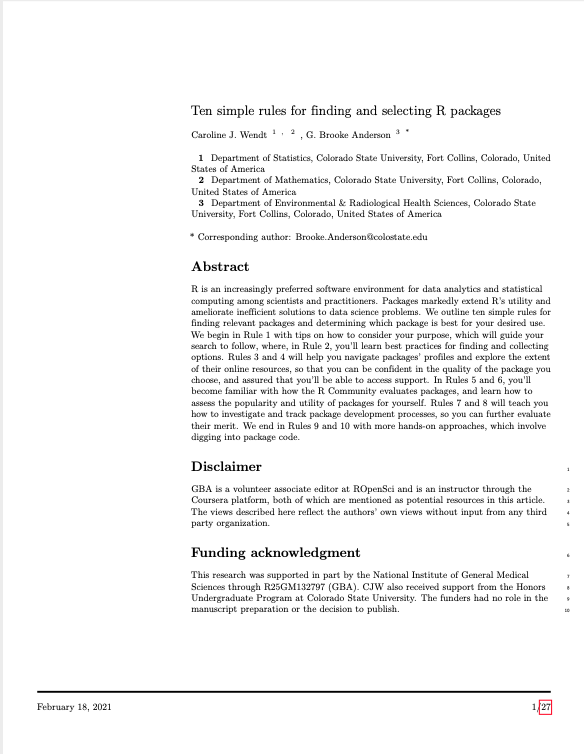
\includegraphics[width=\textwidth]{figures/rticles_example} \textbackslash caption{[}Example of a manuscript written in Rmarkdown using a templat{]}\{Example of a manuscript written in Rmarkdown using a templat. This figure shows the first page of an article written for submission to \emph{PLoS Computation Biology}, written in Rmarkdown while using the \emph{PLoS} template from the \texttt{rticles} package. The full article, including the Rmarkdown input and final pdf, are available on GitHub at \url{https://github.com/cjwendt/plos_ten}.\}\label{fig:rticleexample}
\textbackslash end\{figure\}

These Rmarkdown templates are typically available through R packages, which you
can install on your computer in the same way you would install any R package
(i.e., with the \texttt{install.packages} function). Many journal article templates are
available through the \texttt{rticles} package {[}ref{]}, including the template used to
create the manuscript shown in Figure \ref{fig:rticleexample}. You can find
more information about the \texttt{rticles} package on its GitHub page, at
\url{https://github.com/rstudio/rticles}. There is also a section in the book \emph{R
Markdown: A Definitive Guide} {[}ref{]} on writing manuscripts for scientific
journals using Rmarkdown, available online at
\url{https://bookdown.org/yihui/rmarkdown/rticles-templates.html}.

You can use RMarkdown to create much larger outputs, compared to simpler reports
and protocols. RMarkdown can now be used to create very large and dynamic
documents, including online books (which can also be rendered to pdf versions
suitable for printing), dashboard-style websites, and blogs. Once members of
your research group are familiar with the basics of RMarkdown, you may want to
explore using it to create these more complex outputs. The book format divides
content into chapters and special sections like appendices and references. It
includes a table of contents based on weblinks, so readers can easily navigate
the content. It uses a book format as its base that allows readers to do things
like change the font size and search the book text for keywords. The book
containing these modules is one example of using bookdown. If you would like to
explore using bookdown to create online books based on Rmarkdown files, there
are a number of resources available. There is an online book available with
extensive instructions on using this package, available at
\url{https://bookdown.org/yihui/bookdown/}. There is also a helpful website with more
details on this package, \url{https://bookdown.org/}. The website include a gallery of
example books created with bookdown \url{https://bookdown.org/home/archive/}, which
you can use to explore the types of books that can be created.

You can also use Rmarkdown documents to create webpages, with pages included for
blogs. This format allows you to create a very attractive website that includes
a blog section, where you can write and regularly post new blogs, keeping the
site dynamic. It is a nice entry point to developing and maintaining a website
for people who are learning to code in R but otherwise haven't done much coding,
as you can do all the steps within RStudio. There are templates for these blogs
that are appropriate for creating personal or research group websites for
academics. These websites can be created to highlight the research and people in
your research lab. You can encourage students and postdocs to create personal
sites, to raise the profile of their research. In the past, we have even used
one as a central, unifying spot for a group study, with students contributing
blog posts as their graded assignment
(\url{https://kind-neumann-789611.netlify.app/}). To learn how to create websites with
blogs, you can check the book \emph{blogdown: Creating Websites with R Markdown}
{[}ref{]}, which is available both in print and free online at
\url{https://bookdown.org/yihui/blogdown/}. This process takes a bit of work to
initially get the website set up, but then allows for easy and straightforward
maintenance.

Finally, a simpler way to make basic web content with RMarkdown is through their
\emph{flexdashboard} format. This format creates a smaller website that is focused on
sharing data results---you can see a gallery of examples at
\url{https://rmarkdown.rstudio.com/flexdashboard/examples.html}. This format is
excellent for creating a webpage that allows users to view complex, and
potentially interactive, results from data you've collected. It can be
particularly helpful for groups that need to quickly communicate regularly
updated data to viewers. During 2020, for example, many public health
departments maintained dashboard-style websites to share evolving data on
COVID-19 in the community. Using RMarkdown in this case has the key advantage of
allowing you to easily update the dashboard webpage as you get new or updated
data, since it is easy to re-run any data processing, analysis, and
visualization code in the document. To learn how to use RMarkdown to create
dashboard websites, you can check out RStudio's flexdashboard site at
\url{https://rmarkdown.rstudio.com/flexdashboard/index.html}. There is also guidance
available in one of the chapters of \emph{R Markdown: The Definitive Guide} {[}ref{]}:
\url{https://bookdown.org/yihui/rmarkdown/dashboards.html}.

\textbf{More complex formatting.}

As mentioned earlier, Markdown is a fairly simple markup language. Occasionally,
this simplicity means that you might not be able to create fancier formatting
that you might desire. There is a method that allows you to work around this
constraint in RMarkdown.

In Rmarkdown documents, when you need more complex formatting, you can shift
into a more complex markup language for part of the document. Markup languages
like LaTeX and HTML are much more expressive than Markdown, with many more
formatting choices possible. For example, there is functionality within
LaTeX and HTML to create much more complex tables than in Markdown. However,
there is a downside---when you include formatting specified in these
more complex markup languages, you will limit the output formats that you can
render the document to. For example, if you include LaTeX formatting within
an RMarkdown document, you must output the document to PDF, while if you
include HTML, you must output to an HTML file. Conversely, if you stick with
the simpler formatting available through the Markdown syntax, you can easily
switch the output format for your document among several choices.

The \emph{R Markdown Cookbook} {[}ref{]} includes chapters on how to customize Rmarkdown
output through LaTeX
(\url{https://bookdown.org/yihui/rmarkdown-cookbook/latex-output.html}) and HTML
(\url{https://bookdown.org/yihui/rmarkdown-cookbook/html-output.html}). These
customizations can include creating custom formats for the entire document (for
example, you can customize the appearance of a whole HTML document by
customizing the CSS style file for the document). They can also include
smaller-level customizations, like changing the citation style that is used in
conjunction with a BibTeX file by adding to the preamble for LaTeX output.

One area of customization that is particularly useful and simple to implement is
with customized tables. The Markdown syntax can create very simple tables, but
does not allow the creation of more complex tables. There is an R package called
\texttt{kableExtra} {[}ref{]} that allows you to create very attractive and complex tables
in RMarkdown documents.

This package leverages more of the power of underlying markup languages, rather
than the simpler Markdown language. If you remember, Markdown is pretty easy to
learn because it has a somewhat limited set of special characters and special
markings that you can use to specify formatting in your output document. This
basic set of functionality is often all you need, but for complex table
formatting, you will need more. There is much more available in the deeper
markup languages that you can use specifically to render pdf documents (software
derived from TeX) and the one that you can use specifically to render HTML (the
HTML markup language). As a result, you will need to create RMarkdown files that
are customized to a single output format (pdf or HTML) to take advantage of this
package.

You can install this package the same as any other R package from CRAN, using
\texttt{install.packages}. You will need to use then need to use \texttt{library("kableExtra)}
within your RMarkdown document before you use functions from the package. The
\texttt{kableExtra} package is extensively documented through two vignettes that come
with package, one if the output will be in pdf
(\url{https://cran.r-project.org/web/packages/kableExtra/vignettes/awesome_table_in_pdf.pdf})
and one if it will be in HTML
(\url{https://cran.r-project.org/web/packages/kableExtra/vignettes/awesome_table_in_html.html}).
There is also information on using \texttt{kableExtra} available through \emph{R Markdown
Cookbook} {[}ref{]}: \url{https://bookdown.org/yihui/rmarkdown-cookbook/kableextra.html}.

\hypertarget{learning-more-about-rmarkdown.}{%
\subsection{Learning more about Rmarkdown.}\label{learning-more-about-rmarkdown.}}

To learn more about RMarkdown, you can explore a number of excellent resources.
The most comprehensive are shared by RStudio, where RMarkdown's developer
and maintainer, Yihui Xie, works. These resources are all freely available
online, and some are also available to buy as print books, if you prefer that
format.

First, you should check out the online tutorials that are provided by RStudio on
RMarkdown. These are available at RStudio's RMarkdown page:
\url{https://rmarkdown.rstudio.com/}. The page's ``Getting Started'' section
(\url{https://rmarkdown.rstudio.com/lesson-1.html}) provides a nice introduction you
can work through to try out RMarkdown and practice the overview provided in the
last subsection of this module. The ``Articles'' section
(\url{https://rmarkdown.rstudio.com/articles.html}) provides a number of other
documents to help you learn RMarkdown. RStudio's RMarkdown page also includes a
``Gallery'' (\url{https://rmarkdown.rstudio.com/gallery.html}). This resource allows you
to browse through example documents, so you can get a visual idea of what you
might want to create and then access the example code for a similar document.
This is a great resource for exploring the variety of documents that you can
create using RMarkdown.

To go more deeply into RMarkdown, there are two online books from some of the
same team that are available online. The first is \emph{R Markdown: The Definitive
Guide} by Yihui Xie, J. J. Allaire, and Garrett Grolemund {[}ref{]}. This book is
available free online at \url{https://bookdown.org/yihui/rmarkdown/}. It moves from
basics through very advanced functionality that you can implement with
RMarkdown, including several of the topics we highlight later in this
subsection.

The second online book to explore from this team is \emph{R Markdown Cookbook}, by
Yihui Xie, Christophe Dervieux, and Emily Riederer {[}ref{]}. This book is available
free online at \url{https://bookdown.org/yihui/rmarkdown-cookbook/}. This book is a
helpful resource for dipping in to a specific section when you want to learn how
to achieve a specific task. Just like a regular cookbook has recipes that you
can explore and use one at a time, this book does not require a comprehensive
end-to-end read, but instead provides ``recipes'' with advice and instructions for
doing specific things. For example, if you want to figure out how to align a
figure that you create in the center of the page, rather than the left, you can
find a ``recipe'' in this book to do that.

\hypertarget{applied-exercise-7}{%
\subsection{Applied exercise}\label{applied-exercise-7}}

\begin{quote}
"Most scholarly works have citations and a bibliography or reference section. \ldots{}
The purpose of the bibliography is to provide details of the works that are
cited in the text. We shall refer to cited works as \emph{references}. \ldots{}
The bibliography entries are listed as . The of a reference is also used when the work is
cited in the text. The lists the relevant information
about the work. \ldots{} Even within a single work there may be different styles of
citations. \emph{Parenthetical citations} are usually formed by putting one or
several citation labels inside square brackets or parentheses. However,
there are also other forms of citations that are derived from information in
the citation label. \ldots{} The \texttt{\textbackslash{}bibliographystyle} command tells LaTeX which
style to use for the bibliography {[}e.g., labels as numbers, labels as
names and years{]}. The bibliography style called

, is defined in the
file

.bst. \ldots{} for citations you use the \texttt{\textbackslash{}cite} command. The
argument of the \texttt{\textbackslash{}cite} command is the logical label of the work you cite."
\citep{van2012latex}
\end{quote}

\begin{quote}
``Since bibliographies are important and since it's easy to get them wrong,
some of the work related to the creation of the bibliography has been
automated. This is done by BibTeX. The BibTeX tool requires an external human-readable bibliography database. The database may be viewed as a collection
of records. The record defines the title of the work, the author(s) of the work, the year of publication, and so on. The record also defines the logical
label of the work. This is the label you use when you \texttt{\textbackslash{}cite} the work.
The advantage of using BibTeX is that you provide the information of the
entries in the bibliography and that BibTeX generates the text for the
bibliography. This guarantees consistency and ease of mind. Furthermore,
the BibTeX database is reusable and you may find BibTeX descriptions of
many scholarly works on the web. \ldots{} Generating the bibliography with
BibTex is a multi-stage process, which requires an external program called
bibtex. The bibtex program is to BibTeX what the latex program is to LaTeX.''
\citep{van2012latex}
\end{quote}

\begin{quote}
``You specify the name of the BibTeX database and the location of the
bibliography with the \texttt{\textbackslash{}bibliography} command. The argument of the command
is the basename of the BibTeX database. So if you use \texttt{\textbackslash{}bibliography\{\textless{}db\textgreater{}\}},
then your database is .bib.'' \citep{van2012latex}
\end{quote}

\begin{quote}
``There are several problems with the basic LaTeX citation mechanism.
The \texttt{biblatex} package overcomes many of these. It provides a more flexible
citation mechanism and lets you configure your own citation style.''
\citep{van2012latex}
\end{quote}

\begin{quote}
``The \texttt{biblatex} package distinguishes between \emph{parenthetical} and
\emph{textual} citations.'' \citep{van2012latex}
\end{quote}

\begin{quote}
``This chapter is an introduction to presenting pictures that are stored in
external files. Historically, this was an important mechanism for importing
pictures. \ldots{} The \texttt{figure} environment is used to present pictures, diagrams,
and graphs. The environment creates a \emph{floating} environment. \emph{Floating}
environments don't allow pagebreaks and they may `float' to a convenient
location in the output document. This mechanism gives LaTeX more freedom to
choose better page breaks for the remaining text. \ldots{} However, it should be
noted that you can also force the typesetting of a floating environment at the
`current' position in the output file. \ldots{} LaTeX gives some control over the
placement of floating figures, of floating tables, and other floats. For figures
the placement is controlled with an optional argument of the \texttt{figure}
environment. The same mechanism is used for the \texttt{table} environment\ldots{} The
optional argument, which controls the placement, may contain any combination of
the letters \texttt{t} {[}top of the page{]}, \texttt{b} {[}bottom of a page{]}, \texttt{p} pseparate page
with no text{]}, \texttt{h} {[}approximately at the current position{]}, and \texttt{H} {[}at the
current position{]} \ldots{} The default value for the optional argument is \texttt{tbp}.
LaTeX parses the letters in the optional argument from left to right and puts
the figure at the position corresponding to the first letter for which it thinks
the position is `reasonable'. Good positions are the top of the page, the bottom
of the page, or a page with floats only, because these positions do not disturb
the running text too much.'' \citep{van2012latex}
\end{quote}

\begin{quote}
``We have already seen how to present information in \texttt{tabular} environments.
The \texttt{table} environment creates a \emph{floating} table. As with the \texttt{figure}
environment, this puts the body of the environment in a numbered table,
which may be put in a different place in the document than where it's
actually defined. The table placement is controlled with an optional argument.
This optional argument works as with the optional argument of the
\texttt{figure} environment.'' \citep{van2012latex}
\end{quote}

\begin{quote}
``LaTeX's basic support for mathematics is limited, which is why the
American Mathematical Society (AMS) provides a package called \texttt{amsmath},
which redefines some existing commands and environments and provides
additional commands and environments for mathematical
typesetting.'' \citep{van2012latex}
\end{quote}

\begin{quote}
``LaTeX has three basic modes that determine how it typesets its input.
These modes are: \textbf{text mode} In this mode the output does not have mathematical
content and is typeset as text. \ldots{} \textbf{ordinary math mode} In this mode the
output has mathematical content and is typeset in the running text. Ordinary
math mode is more commonly referred to as inline math mode. \textbf{display math
mode} In this mode the output has mathematical content and is typeset in a
display.'' \citep{van2012latex}
\end{quote}

\begin{quote}
``The \texttt{\$} operator switches from text mode to ordinary math mode and back\ldots{}
The mathematical expressions in the output are typeset in the running text.''
\citep{van2012latex}
\end{quote}

\begin{quote}
``The \texttt{equation} environment is for typesetting a \emph{single} numbered
displayed equation. It is one of the most commonly used environments for
typesetting display math material.'' \citep{van2012latex}
\end{quote}

LaTeX math typesetting includes \citep{van2012latex}:

\begin{itemize}
\tightlist
\item
  subscripts and superscripts
\item
  Greek letters
\item
  text in formulae
\item
  aligned sets of equations
\item
  delimiters (parentheses, brackets)
\item
  fractions
\item
  sums, products, integration, differentiation
\item
  square roots
\item
  relational symbols (less than or equal to, greater than or equal to symbols)
\item
  arrows
\item
  matrices
\item
  accents, hats, dots, overlines
\end{itemize}

\begin{quote}
``This chapter introduces the \texttt{beamer} class, which is widely used for
computer presentations. Some people call such presentations \emph{powerpoint
presentations}. The beamer class is seamlessly integrated with the \texttt{tikz}
package and lets you present \emph{incremental} presentations, which are
presentations that incrementally add text and graphics to a page of the
presentation.'' \citep{van2012latex}
\end{quote}

\begin{quote}
``In May 1977, Donald Knuth of Stanford University started work on the
text-processing system that is now know as 'TeX and METAFONT. \ldots{} In the early
1990s, Donald Knuth officially announced that TeX would not undergo any further
development in the interest of stability. Perhaps unsurprisingly, the 1990s saw
a flowering of experimental projects that extended TeX in various directions;
many of these are coming to fruition in the early 21st century\ldots{}''
\citep{mittelbach2004latex}
\end{quote}

\begin{quote}
The development of TeX from its birth as one of Don's `personal productivity
tools' (created simply to ensure the rapid completion and typographic quality
of his then-current work on \emph{The Art of Computer Programming}) was largely
influenced and nourished by the American Mathematical Society on behalf of
UL research mathematicians." \citep{mittelbach2004latex}
\end{quote}

\begin{quote}
``The most obviously important files in any LaTeX-based documentation project
are the \emph{input source files}. Typically, there will be a master file that uses
other subsidiary files\ldots{} These files most often have the extension \texttt{.tex}\ldots{}
they are commonly known as `plain text files' since they can be prepared with a basic text editor. Often, external graphical images are included in the typeset document utilizing the \texttt{graphics} interface\ldots{} LaTeX also needs several files
containing structure and layout definitions: \emph{class} files with the extension
\texttt{.cls}; \emph{option} files with the extension \texttt{.clo}; \emph{package} files with the
extension \texttt{.sty}\ldots{} Many of these are provided by the base system set-up, but
others may be supplied by individual users.'' \citep{mittelbach2004latex}
\end{quote}

\begin{quote}
``One of the ideas behind LaTeX is the separation between layout and structure
(as far as possible), which allows the user to concentrate on content rather
than having to worry about layout issues.'' \citep{mittelbach2004latex}
\end{quote}

\begin{quote}
``Commands placed between \texttt{\textbackslash{}documentclass} and \texttt{\textbackslash{}begin\{document\}} are in
the so-called \emph{document preamble}. All style parameters must be defined in this
preamble, either in package or class files or directly in the document \emph{before}
the \texttt{\textbackslash{}begin\{document\}} command, which sets the values for some of the global
parameters.'' \citep{mittelbach2004latex}
\end{quote}

\begin{quote}
``Basic LaTeX offers excellent mathematical typesetting capabilities
for straightforward documents. However, when complex displayed equations or
more advanced mathematical constructs are heavily used, something more is
needed. Although it is possible to define new commands or environments to
ease the burden of typing in formulas, this is not the best solution.
The American Mathematical Society (AMS) provides a major package, \texttt{amsmath},
which makes the preparation of mathematical documents much less time-consuming
and more consistent.'' \citep{mittelbach2004latex}
\end{quote}

\begin{quote}
``Citations are cross-references to bibliographical information outside
the current document, such as to publications containing further information
on a subject and source information about used quotations. \ldots{} There are
numerous ways to compile bibliographies and reference lists. They can be
prepared manually, if necessary, but usually they are automatically
generated from a database containing bibliographical infromation\ldots{}''
\citep{mittelbach2004latex}
\end{quote}

\begin{quote}
``There are four common methods of referring to sources: the `short-title',
`author-date', `author-number', and `number-only' systems.'' \citep{mittelbach2004latex}
\end{quote}

\begin{quote}
``The standard LaTeX environment for generating a list of references or a
bibliographyu is called \texttt{thebibliography}. In its default implementation it
automatically generates an appropriate heading and implements a vertical
list structure in which every publication is represented as a separate item.''
\citep{mittelbach2004latex}
\end{quote}

\begin{quote}
``Inside a document, publications are cited by referring to the \emph{cite-key}
argument of the \texttt{\textbackslash{}bibitem} commands. For this purpose LaTeX offers the \texttt{\textbackslash{}cite}
command, which takes such a key as its argument. It can, in fact, take a
comma-separated list of such keys and offers an optional argument to specify
additional information such as page or chapter numbers.'' \citep{mittelbach2004latex}
\end{quote}

\begin{quote}
``The BibTeX program gathers all citation keys used in a document, looks them
up in a bibliographical database, and generates a complete \texttt{thebibliography}
environment that can be loaded by LaTeX in a subsequent run.'' \citep{mittelbach2004latex}
\end{quote}

\begin{quote}
``\ldots{} the basic structure of a BibTeX entry consists of three parts: 1.
A publication \emph{entry type} (e.g., `book', `article', `inproceedings',
`phdthesis'). 2. A \emph{user-chosen keyword} identifying the publication. If you
want to reference the entry in your document, then the argument \emph{cite-key}
of the \texttt{\textbackslash{}cite} command should be identical (also in case) to this keyword.
3. A \emph{series of fields} consisting of a field identifier with its data between
quotes or curly braces (e.g., `author', `journal', and `title').'' \citep{mittelbach2004latex}
\end{quote}

\begin{quote}
``BibTeX entries are read by BibTeX in the bibliography database (the \texttt{.bib}
file), and the formatting of the entries is controlled by an associated
bibliography style (the \texttt{.bst} file), which contains a set of instructions
written in a stack-based language.'' \citep{mittelbach2004latex}
\end{quote}

\begin{quote}
``The BibTeX program was designed by Oren Patashnik to provide a flexible
solution to the problem of automatically generating bibliography lists conforming to different layout styles. It automatically detects the citation requests in
a LaTeX document (by scanning its .aux file or files), selects the needed
bibliographical information from one or more specified databases, and formats
it according to a specified layout style. Its output is a file containing
the bibliography listing as LaTeX code that will be automatically loaded and
used by LaTeX on the following run.'' \citep{mittelbach2004latex}
\end{quote}

\begin{quote}
``A BibTeX database is a plain text (ASCII) file that contains bibliographical
entries internally structured as keyword/value pairs. \ldots{} Each entry in a
BibTeX database consists of three main parts: a \emph{type} specifier, followed
by a \emph{key}, and finally the \emph{data} for the entry itself. The \emph{type} describes
the general nature of the entry (e.g., whether it is an article, book, or
some other publication). The \emph{key} is used in the interface to LaTeX; it
is the string that you have to place in the argument of a \texttt{\textbackslash{}cite} command when
referencing that particular entry. The \emph{data} part consists of a series of
\emph{field entries} depending on the \emph{type}), which can have one of two forms\ldots{}
The comma is the field separator. Spaces surrounding the equals sign or the
comma are ignored. Inside the text part of a field (enclosed in a pair of
double quotes or a pair of braces) you can have any string of characters,
but braces must be matched. The quotes or braces can be omitted for text
consisting entirely of numbers (like the year field\ldots). \ldots{} BibTeX \emph{ignores}
the case of the letters for the entry type, key, and field names. You must,
however, be careful with the key. LaTeX honors the case of the keys specifically
as the argument for a \texttt{\textbackslash{}cite} command, so the key for a given bibliographic
entry must match the one specified in the LaTeX file.'' \citep{mittelbach2004latex}
\end{quote}

\begin{quote}
``Various organizations and individuals have developed style files for
BibTeX that correspond to the house style of particular journals or editing
houses.'' \citep{mittelbach2004latex}
\end{quote}

\begin{quote}
``The document format `R Markdown' was first introduced in the \texttt{knitr}
package in early 2012. The idea was to embed code chunks (of R or other
languages) in Markdown documents. In fact, \texttt{knitr} supported several
authoring languages from the beginning in addition to Markdown, including
LaTeX, HTML, AsciiDoc, reStructuredText, and Textile. Looking back over
the five years, it seems to be fair to say that Markdown has become the
most popular document format, which is what we expected. The simplicity
of Markdown clearly stands out among these document formats.'' \citep{xie2018r}
\end{quote}

\begin{quote}
``However, the original version of Markdown invented by John Gruber was
often found overly simple and not suitable to write highly technical
documents. For example, there was no syntax for tables, footnotes,
math expressions, or citations. Fortunately, John MacFarlane created a
wonderful package named Pandoc to convert Markdown documents (and many
other types of documents) to a large variety of output formats. More
importantly, the Markdown syntax was significantly enriched.
Now we can write more types of elements with Markdown while still enjoying
its simplicity.'' \citep{xie2018r}
\end{quote}

\begin{quote}
``In a nutshell, R Markdown stands on the shoulders of \texttt{knitr} and Pandoc.
The former executes the computer code embedded in Markdown, and converts
R Markdown to Markdown. The latter renders Markdown to the output format
you want (such as PDF, HTML, Word, and so on.).'' \citep{xie2018r}
\end{quote}

\begin{quote}
``R Markdown may not be the right format for you if you find these elements
not enough for your writing: paragraphs, (section) headers, block quotations,
code blocks, (numbered and unnumbered) lists, horizontal rules, tables, inline
formatting (emphasis, strikeout, superscripts, subscripts, verbatim, and
small caps text), LaTeX math expressions, equations, links, images, footnotes,
citations, theorems, proofs, and examples. We believe this list of elements
suffice for most technical and non-technical documents.'' \citep{xie2018r}
\end{quote}

\begin{quote}
``Please do not underestimate the customizability of R Markdown because of the
simplicity of its syntax. In particular, Pandoc templates can be surprisingly
powerful, as long as you understand the underlying technologies such as LaTeX and
CSS, and are willing to invest time in the appearance of your output
documents (reports, books, presentations, and / or websites).'' \citep{xie2018r}
\end{quote}

\begin{quote}
``R Markdown documents are often portable in the sense that they can be
compiled to multiple types of output formats. Again, this is mainly due to the
simplified syntax of the authoring language, Markdown. The simpler the elements
in your document are, the more likely that the document can be converted to
different formats. Similarly, if you heavily tailor R Markdown to a specific
output format (e.g., LaTeX), you are likely to lose the portability, because not
all features in one format work in another format.'' \citep{xie2018r}
\end{quote}

\begin{quote}
``Last but not least, your computing results will be more likely to be
reproducibly if you use R Markdown (or other \texttt{knitr}-based source documents),
compared to the manual cut-and-paste approach. This is because the results
are dynamically generated from computer source code. If anything goes wrong
or needs to be updated, you can simply fix or update the source code, compile
the document again, and the results will automatically be updated. You can
enjoy reproducibility and convenience at the same time.'' \citep{xie2018r}
\end{quote}

\begin{quote}
``There is a fundamental assumption underneath R Markdown that users should
be aware of: we assum it suffices that only a limited number of features are
supported in Markdown. By `features', we mean the types of elements you can
create with native Markdown. The limitation is a great feature, not a bug.''
\citep{xie2018r}
\end{quote}

\begin{quote}
``R Markdown provides an authoring framework for data science. You can use a
single R Markdown file to both: save and execute code, and; generate high
quality reports that can be shared with an audience. R Markdown was designed
for easier reproducibility, since both the computer code and narratives
are in the same document, and results are automatically
generated from the source code.'' \citep{xie2018r}
\end{quote}

\begin{quote}
``There are three basic components of an R Markdown document: the
metadata, text, and code. The metadata is written between the pair of
three dashes \texttt{-\/-\/-}. The syntax for the metadata is YAML (YAML Ain't Markup
Language), so sometimes it's also called the YAML metadata or the YAML
frontmatter. Before it bites you hard, we want to warn you in advance
that indentation matters in YAML, so do not forget to indent the sub-fields
of a top field properly. \ldots{} The body of a document follows the metadata.
The syntax for text (also known as prose or narratives) is Markdown\ldots{}
There are two types of computer code\ldots{} a code chunk starts with three
backticks \ldots{} and ends with three backticks\ldots{} An inline R code expressions
starts with \texttt{\textasciigrave{}r} and ends with a backtick.'' \citep{xie2018r}
\end{quote}

\begin{quote}
``It is fine for humans to err (in computing), as long as the source code
is readily available.'' \citep{xie2018r}
\end{quote}

\begin{quote}
``The idea {[}of R Markdown{]} should be simple enough: interweave narratives
with code in a document, knit the document to dynamically generate results
from the code, and you will get a report. This idea was not generated by
R Markdown, but came from an early programming paradigm called `Literate
Programming' (Knuth, 1984).'' \citep{xie2018r}
\end{quote}

\begin{quote}
``The text in an R Markdown document is written with the Markdown syntax.
Precisely speaking, it is Pandoc's Mardown. There are many flavors of
Markdown invented by different people, and Pandoc's flavor is the
most comprehensive one to our knowledge.'' \citep{xie2018r}
\end{quote}

Markdown syntax allows: inline formatting (e.g., italics, subscript,
superscript), hyperlinks, including images from external files, footnotes,
bibliographical referencing, section headers, \ldots{} \citep{xie2018r}

\begin{quote}
``There are multiple ways to insert citations {[}in Markdown{]}, and we
recommend that you use BibTeX databases, because they work better when
the output format is LaTeX / PDF. \ldots{} The key idea is that when you have
a BibTeX database (a plain-text file with the conventional filename extension
\texttt{.bib}) that contains entries like \ldots{} you may add a field named
\texttt{bibliography} to the YAML metadata, and set its value to the path of the
BibTeX file. Then in Markdown, you may use \texttt{@R-base} \ldots{} to reference the
BibTeX entry. Pandoc will automatically generate a list of references in the
end of the document.'' \citep{xie2018r}
\end{quote}

\begin{quote}
``In general, you'd better leave at least one empty line between adjacent
but different elements, e.g., a header and a paragraph. This is to avoid
ambiguity to the Markdown renderer.'' \citep{xie2018r}
\end{quote}

\begin{quote}
``Inline LaTeX equations can be written in a pair of dollar signs using the
LaTeX syntax\ldots{}'' \citep{xie2018r}
\end{quote}

\begin{quote}
``There are a lot of things you can do in a code chunk: you can produce
text output, tables, or graphics. You have fine control over all these output
via chunk options, which can be provided inside the curly braces. \ldots{} There are
a large number of chunk options in \texttt{knitr} document at \url{https://yihui.name/knitr/options}. We list a subset of them below {[}eval, echo, results, collapse, warning, message, error, include, cache, fig.width, fig.height, out.width, out.height, fig.align, dev, fig.cap{]}.'' \citep{xie2018r}
\end{quote}

\begin{quote}
``Chunk options in \texttt{knitr} can be surprisingly powerful. For example,
you can create animations from a series of plots in a code chunk.'' \citep{xie2018r}
\end{quote}

\begin{quote}
``If caching is enabled the same code chunk will not be evaluated the next
time the document is compiled (if the code chunk was not modified), which can
save you time. However, I want to honestly remind you of the two hard problems
in computer science (via Phil Karlton): naming things, and cache invalidation.
Caching can be handy but also tricky sometimes.'' \citep{xie2018r}
\end{quote}

\begin{quote}
``PDF documents are generated thorugh the LaTeX files generated from R
Markdown. A highly surprising fact to LaTeX beginners is that figures float
by default: even if you generate a plot in a code chunk on the first page,
the whole figure environment may float to the next page. This is just how
LaTeX works by default. It has a tendency to float figures to the top or
bottom of pages. Although it can be annoying and distracting, we recommend
that you refrain from playing the `Whac-A-Mole' game in the beginning of your
writing, i.e., desparately trying to position figures `correctly' while
they seem to be always dodging you. You may wish to fine-tune the positions
once the content is complete using the \texttt{fig.pos} chunk option.'' \citep{xie2018r}
\end{quote}

\begin{quote}
``Formatting tables can be a very complicated task, especially when certain
cells span more than one column or row. It is even more complicated when you
have to consider different output formats. For example, it is difficult to make
a complex table work for both PDF and HTML output.'' \citep{xie2018r}
\end{quote}

\begin{quote}
``A less well-known fact about R Markdown is that many other languages are also
supported, such as Python, Julia, C++, and SQL. The support comes from the
\texttt{knitr} package, which has provided a large number of \emph{language engines}.
Language engines are essentially functions registered in the object
\texttt{knitr::knit\_engine}. \ldots{} To use a different language engine, you can change the
language name in the chunk headerf rom \texttt{r} to the engine name\ldots{} For engines
that rely on external interpreters such as \texttt{python}, \texttt{perl}, and \texttt{ruby}, the
default interpreters are obtained from \texttt{Sys.which()}, i.e., using the
interpreter found via the environment variable \texttt{PATH} of the system. If you want
to use an alternative interpreter, you may specify its path in the chunk option
\texttt{engine.path}. \ldots{} Most engines will execute each code chunk in a separate new
session (via a \texttt{system()} call in R), which means objects created in memory in a
previous code chunk will not be directly available to latter code chunks. \ldots{}
Currently, the only expections are \texttt{r}, \texttt{python}, and \texttt{julia}. Only these
engines execute code in the same session throughout the document. To clarify,
all \texttt{r} code chunks are executed in the same R session, all \texttt{python} code chunks
are executed in the same Python session, and so on, by \emph{the R session and the
Python session are independent.}'' \citep{xie2018r}
\end{quote}

\begin{quote}
``You can also write Shell scripts in R Markdown, if your system can run them
(the executable \texttt{bash} or \texttt{sh} should exist). Usually this is not a problem for
Linux or macOS users. It is not impossible for Windows users to run Shell scripts, but you will have to install additional software (such as Cygwin or the Linux Subsystem).'' \citep{xie2018r}
\end{quote}

\begin{quote}
``R Markdown documents can also generate interactive content. THere are two
types of interactive R Markdown documents: you can use the HTML Widgets
framework, or the Shiny framework (or both). \ldots{} The HTML Widgets framework is
implemented in the R package \texttt{htmlwidgets}, interfacing JavaScript libraries
that create interactive applications, such as interactive graphics and tables.
\ldots{} The \texttt{shiny} package builds interactive web apps powered by R. \ldots{} You may
use Shiny to run any R code that you like in response to user actions. Since web
browsers cannot execute R code, Shiny interactions occur on the server side and
rely on a live R session. By comparison, HTML widgets do not require a live R
session to support them, because the interactivity comes from the client side
(via JavaScript in the web browser).'' \citep{xie2018r}
\end{quote}

\begin{quote}
``By default, MathJax scripts are included in HTML documents for rendering LaTeX and MathML equations.'' \citep{xie2018r}
\end{quote}

\begin{quote}
``Within R Markdown documents that generate PDF output, you can use raw LaTeX, and even define LaTeX macros. See Pandoc's documentation on the raw\_tex extension for details.'' \citep{xie2018r}
\end{quote}

\begin{quote}
``By default, citations are processed through \texttt{pandoc-citeproc}, which works for all output formats. For PDF output, sometimes it is better to use LaTeX packages to process citations, such as \texttt{natbib} or \texttt{biblatex}. To use one of these packages, just set the option \texttt{citation\_package} {[}in the YAML{]}.'' \citep{xie2018r}
\end{quote}

\begin{quote}
``Dashboards are particularly common in business-style reports. THey can
be used to highlight brief and key summaries of a report. THe layout of
a dashboard is often grid-based, with components arranged in boxes of various
sizes.'' \citep{xie2018r}
\end{quote}

\begin{quote}
``Most R Markdown applications are single documents. That is you, have a
single R Markdown source document, and it generates a single output file.
However, it is also possible to work with multiple Rmd documents in a
project, and organize them in a meaningful way (e.g., pages can
reference each other). Currently there are two major ways to build
multiple Rmd documents: blogdown for building websites, and bookdown for
authoring books.'' \citep{xie2018r}
\end{quote}

\begin{quote}
``With blogdown, you can write a blog post or a general page in an Rmd
document, or a plain Markdown document. These source documents will be
built into a static webset, which is essentially a folder containing static
HTML files and associated assets (such as images and CSS files). You
can publish this folder to any web server as a website. Because it is
only a single folder, it can be easy to maintain. \ldots{} Because the website
is generated from R Markdown, the content is more likely to be reproducible,
and also easier to maintain (no cut-and-paste results). Using Markdown
means your content could be more protable in the sense that you may convert
your pages to PDF or other formats in the future, and you are not tied to the
default HTML format.'' \citep{xie2018r}
\end{quote}

\begin{quote}
``Academic journals often have strict guidelines on the formatting for
submitted articles. As of today, few journals directly support R
Markdown submissions, but many support the LaTeX format. While you can
convert R Markdown to LaTeX, different journals have different
typesetting requirements and LaTeX styles, and it may be slow and
frustrating for all authors who want to use R Markdown to figure out
the technical details about how to properly convert a paper based on
R Markdown to a LaTeX document that meets the journal requirements. The
rticles package is designed to simplify the creation of documents that
conform to submission standards. A suite of custom R Markdown templates
for popular journals is provided\ldots{} Understanding of LaTeX is recommended,
but not essential, to use this package. R Markdown templates may sometimes
inevitably contain LaTeX code, but usually we can use the simpler Markdown
and knit syntax to produce elements like figures, tables, and
math equations\ldots{}'' \citep{xie2018r}
\end{quote}

The \texttt{rticles} package includes templates for the Elsevier and Springer
family of journals.

\hypertarget{module20}{%
\section{Example: Creating a reproducible data pre-processing protocol}\label{module20}}

We will walk through an example of creating a reproducible data pre-processing
protocol. As an example, we will use the pre-processing task required for
estimating the bacterial load from plating samples from an immunological
experiment at serial dilutions, using data from an experiment lead by one of the
coauthors. This data pre-processing protocol was created using RMarkdown and
allows the efficient, transparent, and reproducible pre-processing of plating
data for all experiments in the research group. We will go through how RMarkdown
techniques can be applied to develop this type of data pre-processing protocol
for a laboratory research group.

\textbf{Objectives.} After this module, you should be able to:

\begin{itemize}
\tightlist
\item
  Explain how a reproducible data pre-processing protocol can be developed for
  a real research project
\item
  Understand how to design and implement a data pre-processing protocol to
  replace manual or point-and-click data pre-processing tools
\item
  Apply techniques in RMarkdown to develop your own reproducible data
  pre-processing protocols
\end{itemize}

\hypertarget{introduction-and-example-data}{%
\subsection{Introduction and example data}\label{introduction-and-example-data}}

In this module, we'll provide advice and an example of how you can use the
tools for knitted documents to create a reproducible data preprocessing
protocol. This module builds on ideas and techniques that were introduced
in the last two modules, to help you put them into practical use for
data preprocessing that you do repeatedly for research data in your
laboratory.

In this module, we will use an example of a common pre-processing task in
immunological research: estimating the bacterial load in samples by plating at
different dilutions, identifying a good dilution for counting colony-forming
units (CFUs), and then back-calculating the estimated bacterial load in the
original sample based on the colonies counted at this dilution. This
experimental technique dates back to the late 1800s, with Robert Koch, and
continues to be widely used in microbiology research and applications today
\citep{ben2014estimation}. These data are originally from an experiment in one of our
authors' laboratory and are also available as example data for an R package
called \texttt{bactcountr}, currently under development at
\url{https://github.com/aef1004/bactcountr/tree/master/data}.

These data are representative of data often collected in immunological research.
For example, you may be testing out some drugs against an infectious bacteria
and want to know how successful different drugs are in limiting bacterial load.
You run an experiment and have samples from animals treated with different drugs
or under control and would then want to know how much viable (i.e., replicating)
bacteria are in each of your samples.

You can find out by plating the sample at different dilutions and
counting the colony-forming units (CFUs) that are cultured on each plate.
You put a sample on a plate with a medium they can grow on and then give them
time to grow. The idea is that individual bacteria from the original sample end
up randomly around the surface of the plate, and any that are viable (able to
reproduce) will form a new colony that, after a while, you'll be able to see.

To get a good estimate of bactieral load from this process, you need to count
CFUs on a ``countable'' plate---one with a ``just right'' dilution (and you
typically won't know which dilution this is for a sample until after plating).
If you have too high of a dilution (i.e., one with very few viable bacteria),
randomness will play a big role in the CFU count, and you'll estimate the
original with more variability. If you have too low of a dilution (i.e., one
with lots of viable bacteria), it will be difficult to identify separate
colonies, and they may complete for resources. To translate from diluted
concentration to original concentration, you can then do a back-calculation,
incorporating both the number of colonies counted at that dilution and how
dilute the sample was. There is therefore some pre-processing required (although
it is fairly simple) to prepare the data collected to get an estimate of
bacterial load in the original sample. This estimate can then be used in
statistical testing and combined with other experimental data to explore
questions like whether a candidate vaccine reduces bacterial load.

We will use this example of a common data pre-processing task to show how to
create a reproducible pre-processing protocol in this module. If you would like,
you can access all the components of the example pre-processing protocol and
follow along, re-rendering it yourself on your own computer. The example data
are available as a csv file, downloadable
\href{https://raw.githubusercontent.com/geanders/improve_repro/master/data/bactcountr_example_data/cfu_data.csv}{here}.
You can open this file using spreadsheet software, or look at it directly in
RStudio. The final pre-processing protocol for these data can also be
downloaded, including both \href{https://raw.githubusercontent.com/geanders/improve_repro/master/data/bactcountr_example_data/example_protocol.Rmd}{the original RMarkdown
file}
and \href{https://github.com/geanders/improve_repro/raw/master/data/bactcountr_example_data/example_protocol.pdf}{the output PDF
document}.
Throughout this module, we will walk through elements of this document, to
provide an example as we explain the process of developing data pre-processing
modules for common tasks in your research group.

This example is intentionally simple, to allow a basic introduction to the
process using pre-processing tasks that are familiar to many laboratory-based
scientists and easy to explain to anyone who has not used plating experimental
work. However, the same general process can also be used to create
pre-processing protocols for data that are much larger or more complex or for
pre-processing pipelines that are much more involved.
For example, this process could be used to create data pre-processing protocols
for automated gating of flow cytometry data or for pre-processing data
collected through liquid chromatography--mass spectrometry.

\hypertarget{advice-on-designing-a-pre-processing-protocol}{%
\subsection{Advice on designing a pre-processing protocol}\label{advice-on-designing-a-pre-processing-protocol}}

Before you write your protocol in a knitted document, you should decide on the
content to include in the protocol. This section provides tips on this design
process. In this section, we'll describe some key steps in designing a
data pre-processing protocol:

\begin{enumerate}
\def\labelenumi{\arabic{enumi}.}
\tightlist
\item
  Defining input and output data for the protocol;
\item
  Setting up a project directory for the protocol;
\item
  Outlining key tasks in pre-processing the input data; and
\item
  Adding code for pre-processing.
\end{enumerate}

We will illustrate these design steps using the example protocol on
pre-processing plating data.

\textbf{Defining input and output data for the protocol.}

The first step in designing the data pre-processing protocol is to decide on the
starting point for the protocol (the data input) and the ending point (the data
output). It may make sense to design a separate protocol for each major type of
data that you collect in your research laboratory. Your input data for the
protocol, under this design, might be the data that is output from a specific
type of equipment (e.g., flow cytometer) or from a certain type of sample or
measurement (e.g., metabolomics run on a mass spectrometer), even if it is a
fairly simple type of data (e.g., CFUs from plating data, as used in the example
protocol for this module). For example, say you are working with three types of
data for a research experiment: data from a flow cytometer, metabolomics data
measured with a mass spectrometer, and bacterial load data measured by plating
data and counting colony forming units (CFUs). In this case, you may want to
create three pre-processing protocols: one for the flow data, one for the
metabolomics data, and one for the CFU data. These protocols are modular and can
be re-used with other experiments that use any of these three types of data.

With an example dataset, you can begin to create a pre-processing protocol
before you collect any of your own research data for a new experiment. If the
format of the initial data is similar to the format you anticipate for your
data, you can create the code and explanations for key steps in your
pre-processing for that type of data. Often, you will be able to adapt the
RMarkdown document to change it from inputting the example data to inputting
your own experimental data with minimal complications, once your data comes in.
By thinking through and researching data pre-processing options before the data
is collected, you can save time in analyzing and presenting your project results
once you've completed the experimental data collection for the project. Further,
with an example dataset, you can get a good approximation of the format in which
you will output data from the pre-processing steps. This will allow you to begin
planning the analysis and visualization that you will use to combine the
different types of data from your experiment and use it to investigate important
research hypotheses. Again, if data follow standardized formats across steps in
your process, it will often be easy to adapt the code in the protocol to input
the new dataset that you created, without major changes to the code developed
with the example dataset.

While pre-processing protocols for some types of data might be very complex,
others might be fairly simple. However, it is still worthwhile to develop a
protocol even for simple pre-processing tasks, as it allows you to pass along
some of the details of pre-processing the data that might have become ``common
sense'' to longer-tenured members of your research group. For example, the
pre-processing tasks in the example protocol are fairly simple. This protocol
inputs data collected in a plain-text delimited file (a csv file, in the
example). Within the protocol, there are steps to convert initial measurements
from plating at different dilutions into an estimate of the bacterial load in
each sample. There are also sections in the protocol for exploratory data
analysis, to allow for quality assessment and control of the collected data as
part of the preprocessing. The output of the protocol is a simple data object (a
dataframe, in this example) with the bacterial load for each original sample.
These data are now ready to be used in tables and figures in the research report
or manuscript, as well as to explore associations with the experimental design
details (e.g., comparing bacterial load in treated versus untreated animals) or
merged with other types of experimental data (e.g., comparing immune cell
populations, as measured with flow cytometry data, with bacterial loads, as
measured from plating and counting CFUs).

Once you have identified the input data type to use for the protocol, you should
identify an example dataset from your laboratory that you can use to create the
protocol. This could be a dataset that you currently need to pre-process, in
which case the development of the protocol will serve a second purpose, allowing
you to complete this task at the same time. However, you may not have a new set
of data of this type that you currently need to pre-process, and in this case
you can build your protocol using a dataset from a previous experiment in your
laboratory. In this case, you may already have a record of the steps that you
used to pre-process the data previously, and these can be helpful as a starting
point as you draft the more thorough pre-processing protocol. You may want to
select an example dataset that you have already published or are getting ready
to publish, so you won't feel awkard about making the data available for people
to practice with. If you don't have an example dataset from your own laboratory,
you can explore example datasets that are already available, either as data
included with existing R packages or through open repositories, including those
hosted through national research institutions like the NIH. In this case, be
sure to cite the source of the data and include any available information about
the equipment that was used to collect it, including equipment settings used
when the data were collected.

For the example protocol for this module, we want to pre-process data that were
collected ``by hand'' by counting CFUs on plates in the laboratory. These counts
were recorded in a plain text delimited file (a csv file) using spreadsheet
software. The spreadsheet was set up to ensure the data can easily be converted
to a ``tidy'' format, as described in module 2.3. The first few rows of the input
data look like this:

\begin{verbatim}
## # A tibble: 6 x 6
##   group replicate dilution_0 dilution_1 dilution_2 dilution_3
##   <dbl> <chr>     <chr>      <chr>           <dbl>      <dbl>
## 1     2 2-A       26         10                  0          0
## 2     2 2-B       TNTC       52                 10          5
## 3     2 2-C       0          0                   0          0
## 4     3 3-A       0          0                   0          0
## 5     3 3-B       TNTC       TNTC               30         10
## 6     3 3-C       0          0                   0          0
\end{verbatim}

Each row represents the number of bacterial colonies counted after plating a
certain sample, where each sample represents one experimental animal and several
experimental animals (replicates) were considered for each experimental group.
Columns are included with values for the experimental group of the sample
(\texttt{group}), the specific ID of the sample within that experimental group
(\texttt{replicate}, e.g., \texttt{2-A} is mouse A in experimental group 2), and the
colony-forming units (CFUs) counted at each of several dilutions. If a cell has
the value ``TNTC'', this indicates that CFUs were too numerous to count for that
sample at that dilution.

When you have identified the input data type you will use for the protocol,
as well as selected an example dataset of this type to use to create the
protocol, you can include a section in the protocol
that describes these input data, what file format they are in, and how they
can be read into R for pre-processing (Figure \ref{fig:protocoldatainput}).

\begin{figure*}
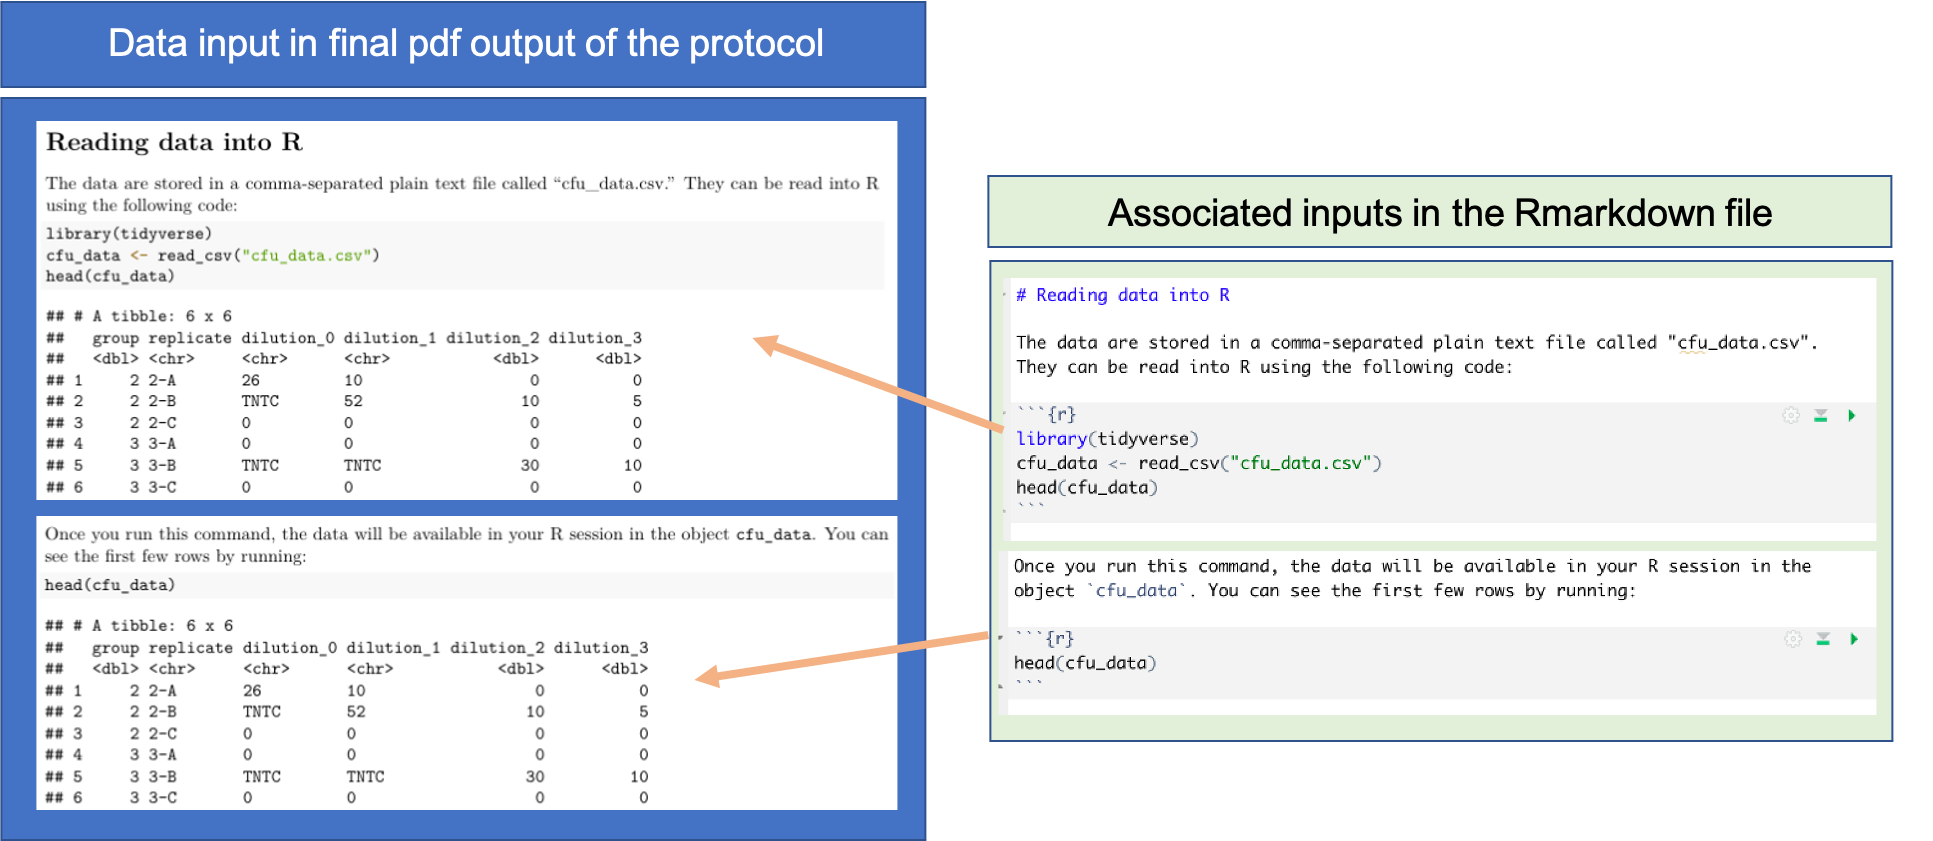
\includegraphics[width=\textwidth]{figures/protocol_data_input} \caption[Providing details on input data in the pre-processing protocol]{Providing details on input data in the pre-processing protocol. Once you have an example data file for the type of data that will be input for the protocol, you can add a section that provides the code to read the data into R. You can also add code that will show the first few rows of the example dataset, as well as a description of the data. This figure shows examples of how these elements can be added to an RMarkdown file for a pre-processing protocol, and the associated elements in the final pdf of the protocol, using the example protocol for this module.}\label{fig:protocoldatainput}
\end{figure*}

For the data output, it often makes sense to plan for data in a format that is
appropriate for data analysis and for merging with other types of data collected
from the experiment. The aim of pre-processing is to get the data from the
format in which they were collected into a format that is meaningful for
combining with other types of data from the experiment and using in statistical
hypothesis testing.

In the example pre-processing protocol, we ultimately
output a simple dataset, with one row for each of the original samples. The
first few rows of this output data are:

\begin{verbatim}
## # A tibble: 6 x 3
##   group replicate cfu_in_organ
##   <dbl> <chr>            <dbl>
## 1     2 2-A                260
## 2     2 2-B               2500
## 3     2 2-C                  0
## 4     3 3-A                  0
## 5     3 3-B               7500
## 6     3 3-C                  0
\end{verbatim}

For each original sample, an estimate of the CFUs of \emph{Mycobacterium
tuberculosis} in the full spleen is given (\texttt{cfu\_in\_organ}). These data
can now be merged with other data collected about each animal in the experiment.
For example, they could be joined with data that provide measures of the
immune cell populations for each animal, to explore if certain immune
cells are associated with bacterial load. They could also be joined with
experimental information and then used in hypothesis testing. For example,
these data could be merged with a table that describes which groups were
controls versus which used a certain vaccine, and then a test could be
conducted exploring evidence that bacterial loads in animals given a
vaccine were lower than in control animals.

\textbf{Setting up a project directory for the protocol}

Once you have decided on the input and output data formats, you will next want
to set up a file directory for storing all the inputs needed in the protocol.
You can include the project files for the protocol in an RStudio Project (see
module 2.6) and post this either publicly or privately on GitHub (see modules
2.9--2.11). This creates a ``packet'' of everything that a reader needs to use to
recreate what you did---they can download the whole GitHub repository and will
have a nice project directory on their computer with everything they need to try
out the protocol.

Part of the design of the protocol involves deciding on the files that should be
included in this project directory. Figure \ref{fig:protocolprojectfiles}
provides an example of the initial files included in the project directory for
the example protocol for this module. The left side of the figure shows the
files that are initially included, while the left side shows the files in the
project after the code in the protocol is run.

Generally, in the project directory you should include a file with the input
example data, in whatever file format you will usually collect this type of
data. You will also include an RMarkdown file where the protocol is written. If
you are planning to cite articles and other references, you can include a BibTeX
file, with the bibliographical information for each source you plan to cite.
Finally, if you would like to include photographs or graphics, you can include
these image files in the project directory. Often, these will be included
together in a subdirectory of the project named something like ``figures''.

Once you run the RMarkdown file for the protocol, you will generate additional
files in the project. Two typical files you will generate will be the output
file for the protocol (in the example, this is output to a pdf file). Usually,
the code in the protocol will also result in output data, which is pre-processed
through the protocol code and written into a file to be used in further
analysis.

\begin{figure}
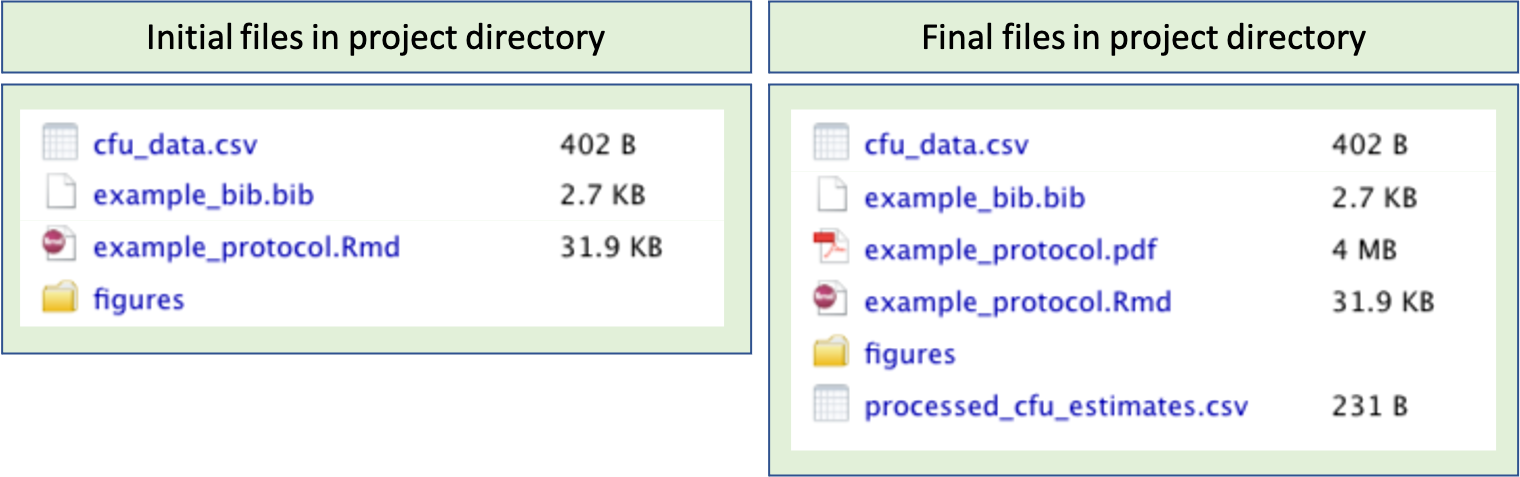
\includegraphics[width=\textwidth]{figures/protocol_project_files} \caption[Example of files in the project directory for a data pre-processing protocol]{Example of files in the project directory for a data pre-processing protocol. On the left are the files initially included in the project directory for the example protocol for this module. These include a file with the input data (cfu\_data.csv), a BibTeX file with bibliographical information for references (example\_bib.bib), the RMarkdown file for the protocol (example\_protocol.Rmd), and a subdirectory with figures to include in the protocol (figures). On the right is shown the directory after the code in the protocol RMarkdown document is run, which creates an output pdf with the protocol as well as the output data (processed\_cfu\_estimates.csv).}\label{fig:protocolprojectfiles}
\end{figure}

\textbf{Outlining key tasks in pre-processing the input data.}

The next step is to outline the key tasks that are involved in moving from the
data input to the desired data output. For the plating data we are using for our
example, the key tasks to be included in the pre-processing protocol are:

\begin{enumerate}
\def\labelenumi{\arabic{enumi}.}
\tightlist
\item
  Read the data into R
\item
  Explore the data and perform some quality checks
\item
  Identify a ``good'' dilution for each sample---one at which you have a
  countable plate
\item
  Estimate the bacterial load in each original sample based on the CFUs counted
  at that dilution
\item
  Output data with the estimated bacterial load for each sample
\end{enumerate}

Once you have this basic design, you can set up the RMarkdown file for the
pre-processing protocol to include a separate section for each task, as well as
an ``Overview'' section at the beginning to describe the overall protocol, the
data being pre-processed, and the laboratory procedures used to collect those
data. In RMarkdown, you can create first-level section headers by putting the
text for the header on its own line and beginning that line with \texttt{\#}, followed
by a space. You should include a blank line before and after the line with this
header text. Figure \ref{fig:protocolsections} shows how this is done in the
example protocol for this module, showing how text in the plain text RMarkdown
file for the protocol align with section headers in the final pdf output of the
protocol.

\begin{figure*}
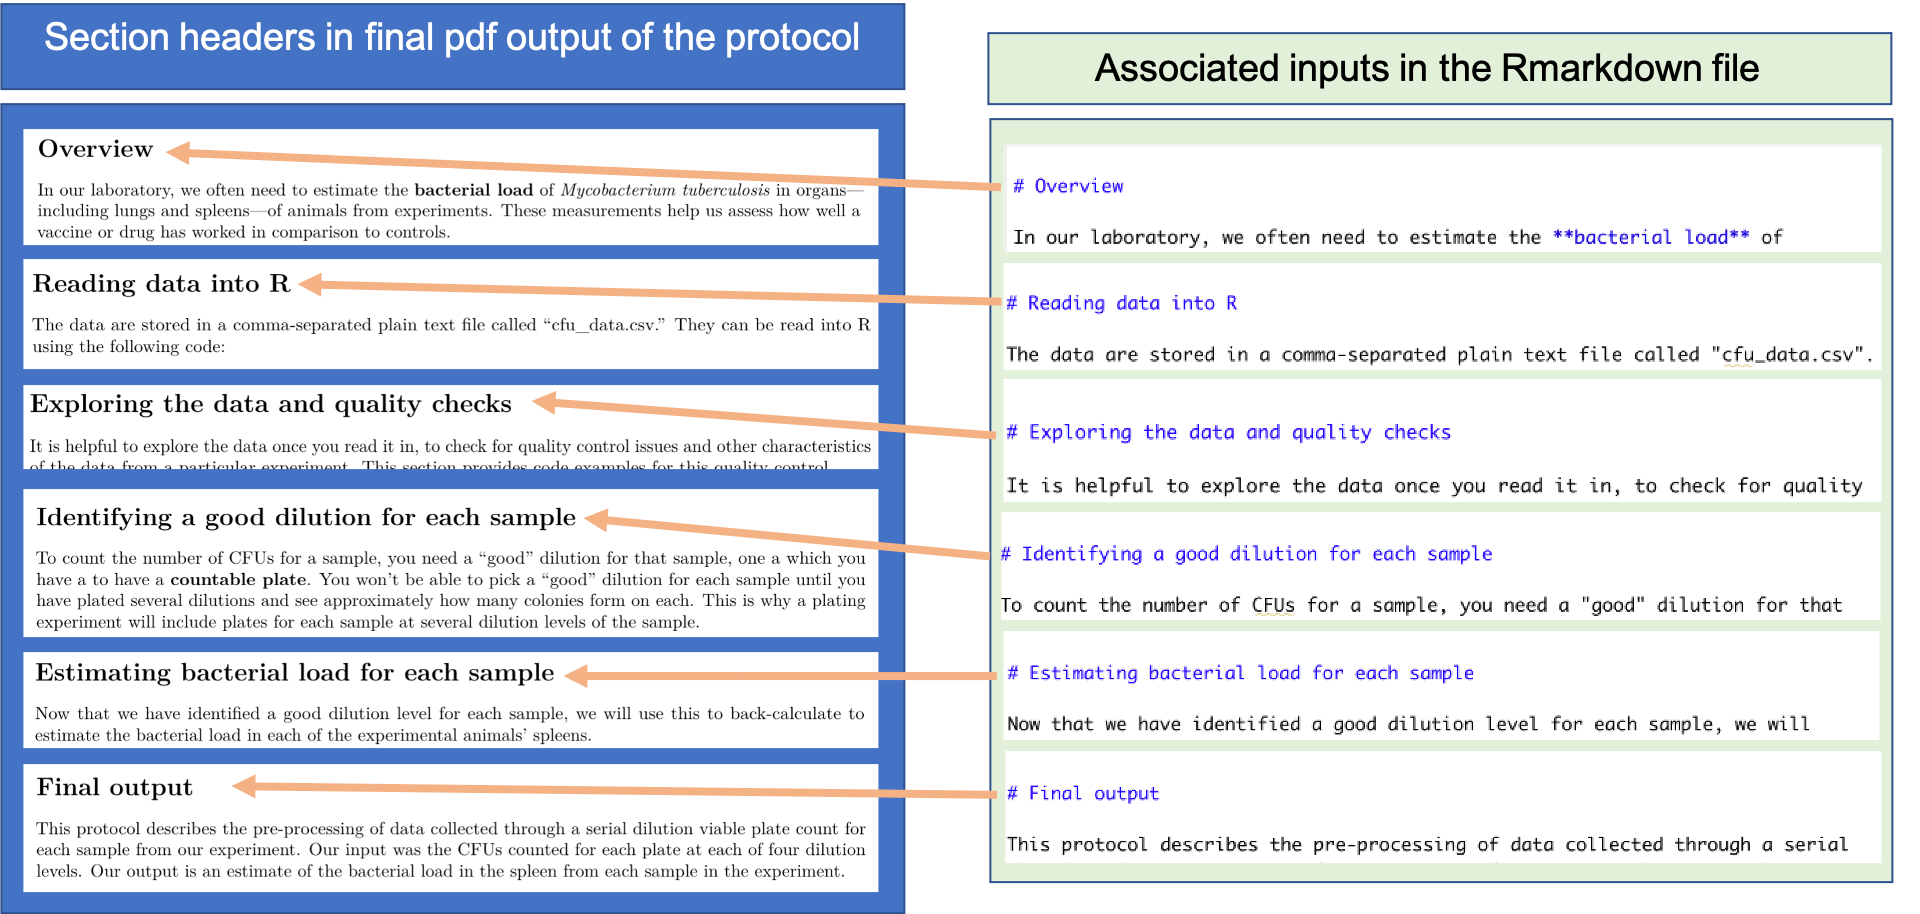
\includegraphics[width=\textwidth]{figures/protocol_sections} \caption[Dividing an RMarkdown data pre-processing protocol into sections]{Dividing an RMarkdown data pre-processing protocol into sections. This shows an example of creating section headers in a data pre-processing protocol created with RMarkdown, showing section headers in the example pre-procotcol for this module.}\label{fig:protocolsections}
\end{figure*}

\textbf{Adding code for pre-processing.}

For many of these steps, you likely have code---or can start drafting the
code---required for that step. If you were doing the pre-processing entirely
through a code script or interactively, you would exclusively write code for the
steps. A good next step, therefore, in designing your pre-protocol is to add in
the code for each step to conduct the pre-processing required in each section.

In RMarkdown, you can test this code as you write it. You insert each piece
of executable code within a special section, separated from the regular
text with special characters, as described in previous modules.

For any pre-processing steps that are straightforward (e.g., calculating the
dilution factor in the example module, which requires only simple mathematical
operations), you can directly write in the code required for the step.
For other pre-processing steps, however, the algorithm may be a bit more
complex. For example, complex algorithms have been developed for steps like
peak identification and alignment that are required when
pre-processing data from a mass spectrometer.

For these more complex tasks, you can start to explore available R packages for
performing the task. There are thousands of packages available that extend the
basic functionality of R, providing code implementations of algorithms in a
variety of scientific fields. Many of the R packages relevant for biological
data---especially high-throughput biological data---are available through a
repository called Bioconductor. These packages are all open-source (so you can
explore their code if you want to) and free. You can use vigettes and package
manuals for Bioconductor packages to identify the different functions you can
use for your pre-processing steps. Once you have identified a function for the
task, you can use the helpfile for the function to see how to use it. This help
documentation will allow you to determine all of the function's parameters and
the choices you can select for each.

You can add each piece of code in the RMarkdown version of the protocol using
the standard method for RMarkdown (module {[}x{]}). Figure \ref{fig:protocolcode}
shows an example from the example protocol for this module. Here, we are using
code to help identify a ``good'' dilution for counting CFUs for each sample. The
code in included in an executable code chunk, and so it will be run each time
the protocol is rendered. Code comments are included in the code to provide
finer-level details about what the code is doing.

\begin{figure*}
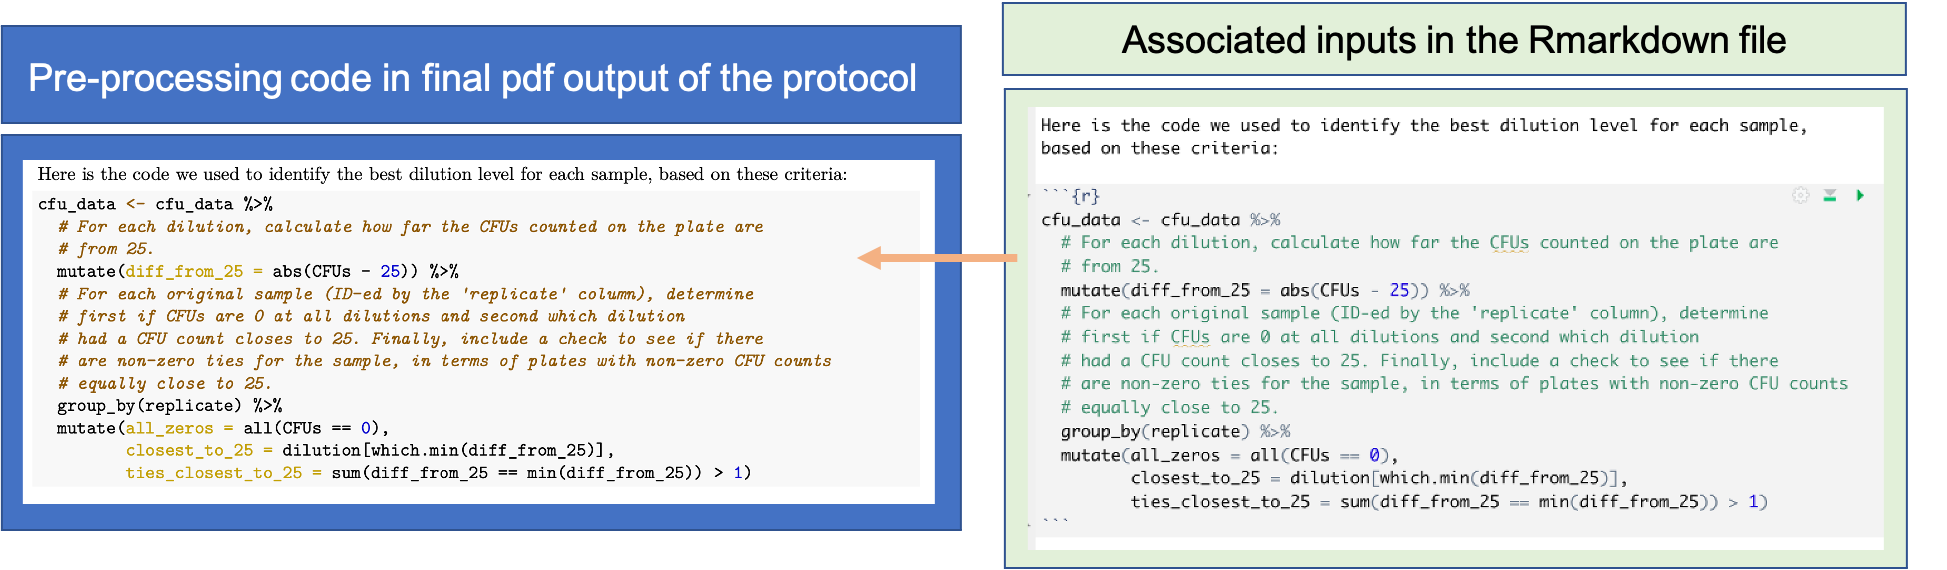
\includegraphics[width=\textwidth]{figures/protocol_code} \caption[Example of including code in a data pre-processing protocol created with RMarkdown]{Example of including code in a data pre-processing protocol created with RMarkdown. This figure shows how code can be included in the RMarkdown file for a pre-processing protocol (right), and the corresponding output in the final pdf of the protocol (left), for the code to identify a 'good' dilution for counting CFUs for each sample. Code comments are included to provide finer-level details on the code.}\label{fig:protocolcode}
\end{figure*}

For each step of the protocol, you can also include potential problems
that might come up in specific instances of the data you get from
future experiments. This can help you adapt the code in the protocol in
thoughtful ways as you apply it in the future to new data collected
for new studies and projects.

\hypertarget{writing-data-pre-processing-protocols}{%
\subsection{Writing data pre-processing protocols}\label{writing-data-pre-processing-protocols}}

Now that you have planned out the key components of the pre-processing protocol,
you can use RMarkdown's functionality to flesh it out into a full pre-processing
protocol. This gives you the chance to move beyond a simple code script, and
instead include more thorough descriptions of what you're doing at each step and
why you're doing it. You can also include discussions of potential limitations
of the approach that you are taking in the pre-processing, as well as areas
where other research groups might use a different approach. These details can
help when it is time to write the Methods section for the paper describing your
results from an experiment using these data. They can also help your research
group identify pre-processing choices that might differ from other research
groups, which opens the opportunity to perform sensitivity analyses regarding
these pre-processing choices and ensure that your final conclusions are robust
across multiple reasonable pre-processing approaches.

Protocols are common for wet lab techniques, where they provide a ``recipe'' that
ensures consistency and reproducibility in those processes. Computational tasks,
including data pre-processing, can also be standardized through the creation and
use of protocol in your research group. While code scripts are becoming more
common as a means of recording data pre-processing steps, they are often not
as clear as a traditional protocol, in particular in terms of providing a
thorough description of what is being done at each step and why it is being
done that way. Data pre-processing protocols can provide these more thorough
descriptions, and by creating them with RMarkdown or with similar types
of ``knitted'' documents (module {[}x{]}), you can combine the executable code
used to pre-process the data with extensive documentation. As a further
advantage, the creation of these protocols will ensure that your research
group has thought carefully about each step of the process, rather than
relying on cobbling together bits and pieces of code they've found but don't
fully understand. Just as the creation of a research protocol for a
clinical trial requires a careful consideration of each step of the ultimate
trial \citep{al2016protocol}, the creation of data pre-processing protocols ensure
that each step in the process is carefully considered, and so helps to
ensure that each step of this process is conducted as carefully as the
steps taken in designing the experiment as a whole and each wet lab technique
conducted for the experiment.

\begin{quote}
``Writing a research proposal is probably one of the most challenging and
difficult task as research is a new area for the majority of postgraduates and
new researchers. \ldots{} Protocol writing allows the researcher to review and
critically evaluate the published literature on the interested topic, plan and
review the project steps and serves as a guide throughout the investigation.''
\citep{al2016protocol}
\end{quote}

A data-preprocessing protocol, in the sense we use it here, is essentially an
annotated recipe for each step in preparing your data from the initial, ``raw''
state that is output from the laboratory equipment (or collected by hand) to a
state that is useful for answering important research questions. The exact
implementation of each step is given in code that can be re-used and adapted
with new data of a similar format. However, the code script is often not enough
to helpfully understand, share, and collaborate on the process. Instead, it's
critical to also include descriptions written by humans and for humans. These
annotations can include descriptions of the code and how certain parameters are
standardized the algorithms in the code. They can also be used to justify
choices, and link them up both with characteristics of the data and equipment
for your experiment as well as with scientific principles that underlie the
choices. Protocols like this are critical to allow you to standardize the
process you use across many samples from one experiment, across different
experiments and projects in your research laboratory, and even across different
research laboratories.

As you begin adding text to your pre-processing protocol, you should keep in
mind these general aims. First, a good protocol provides adequate detail that
another researcher can fully reproduce the procedure \citep{al2016protocol}. For a
protocol for a trial or wet lab technique, this means that the protocol should
allow another researcher to reproduce the process and get results that are
\emph{comparable} to your results \citep{al2016protocol}; for a data pre-processing
protocol, the protocol must include adequate details that another researcher,
provided they start with the same data, gets \emph{identical} results (short of any
pre-processing steps that include some element of sampling or random-number
generation, e.g., Monte Carlo methods). This idea---being able to exactly
re-create the computational results from an earlier project---is refered to as
\textbf{computational reproducbility} {[}ref{]} and is considered a key component in
ensuring that research is fully reproducible {[}ref{]}.

\begin{quote}
``It should provide enough detail (methodology) that can allow another
investigator to do the study and arrive at comparable conclusions.''
\citep{al2016protocol}
\end{quote}

By creating the data pre-processing protocol as a knitted document (module {[}x{]})
using a tool like RMarkdown (module {[}x{]}), you can ensure that the protocol is
computationally reproducible. In an RMarkdown document, you include the code
examples as \emph{executable} code---this means that the code is run every time you
render the document. You are therefore ``checking'' your code every time that you
run it. As the last step of your pre-processing protocol, you should output the
copy of the pre-processed data that you will use for any further analysis for
the project. You can use functions in R to output this to a plain text format,
for example a comma-separated delimited file (module {[}x{]}). Each time you render
the protocol, you will re-write this output file, and so this provides assurance
that the code in your protocol can be used to reproduce your output data (since
that's how you yourself created that form of the data).

Figure \ref{fig:protocoloutput} provides an example from the example protocol
for this module. The RMarkdown file for the protocol includes code to write out
the final, pre-processed data to a comma-separated plain text file called
``processed\_cfu\_estimates.csv''. This code writes the output file into the same
directory where you've saved the RMarkdown file. Each time the RMarkdown file is
rendered to create the pdf version of the protocol, the input data will be
pre-processed from scratch, using the code throughout the protocol, and this
file will be overwritten with the data generated. This guarantees that the code
in the protocol can be used by anyone---you or other researchers---to reproduce
the final data from the protocol, and so guarantees that these data are
computationally reproducible.

\begin{figure*}

\includegraphics[width=\textwidth]{figures/protocol_output_data} \caption[Example of using code in pre-processing protocol to output the final, pre-processed data that will be used in further analysis for the research project]{Example of using code in pre-processing protocol to output the final, pre-processed data that will be used in further analysis for the research project. This example comes from the example protocol for this module, showing both the executable code included in the RMarkdown file for the protocol (right) and how this code is included in the final pdf of the protocol. Outputting the pre-processed data into a plain text file as the last step of the protocol helps ensure computational reproducibility for this step of working with experimental data.}\label{fig:protocoloutput}
\end{figure*}

In your data pre-processing protocol, show the code that you use to implement
this choice and also explain clearly in the text why you made this choice and
what alternatives should be considered if data characteristics are different.
Write this as if you are explaining to a new research group member (or your
future self) how to think about this step in the pre-processing, why you're
doing it the way your doing it, and what code is used to do it that way. You
should also include references that justify choices when they are
available---include these using BibTex. By doing this, you will make it much
easier on yourself when you write the Methods section of papers that report on
the data you have pre-processed, as you'll already have draft information on
your pre-processing methods in your protocol.

Good protocols include not only \emph{how} (for data pre-processing protocols, this
is the code), but also \emph{why} each step is taken. This includes both higher-level
(i.e., what a larger question is being asked) and also at a fine level, for each
step in the process. A protocol should include some background, the
aims of the work, hypotheses to be tested, materials and methods, methods of
data collection and equipment to analyze samples \citep{al2016protocol} (This
reference is discussing full protocols for a study, e.g., a clinicial trial, so
includes more steps that just pre-processing.)

This step of documentation and explanation is very important to creating a
useful data pre-processing protocol. Yes, the code itself allows someone else to
replicate what you did. However, only those who are very, very familiar with the
software program, including any of the extension packages you include, can
``read'' the code directly to understand what it's doing. Further, even if you
understand the code very well when you create it, it is unlikely that you will
stay at that same level of comprehension in the future, as other tasks and
challenges take over that brain space. Explaining for humans, in text that
augments and accompanies the code, is also important because function names and
parameter names in code often are not easy to decipher. While excellent
programmers can sometimes create functions with clear and transparent names,
easy to translate to determine the task each is doing, this is difficult in
software development and is rare in practice. Human annotations, written by and
for humans, are critical to ensure that the steps will be clear to you and
others in the future when you revisit what was done with this data and what you
plan to do with future data.

The process of writing a protocol in this way forces you to think about each
step in the process, why you do it a certain way (include parameters you choose
for certain functions in a pipeline of code), and include justifications from
the literature for this reasoning. If done well, it should allow you to quickly
and thoroughly write the associated sections of Methods in research reports and
manuscripts and help you answer questions and challenges from reviewers. Writing
the protocol will also help you identify steps for which you are uncertain how
to proceed and what choices to make in customizing an analysis for your research
data. These are areas where you can search more deeply in the literature to
understand implications of certain choices and, if needed, contact the
researchers who developed and maintained associated software packages to get
advice.

For example, the example protocol for this module explains how to pre-process
data collected from counting CFUs after plating serial dilutions of samples. One
of the steps of pre-processing is to identify a dilution for each sample at
which you have a ``countable'' plate. The protocol includes an explanation of why
it is important to identify the dilution for a countable plate and also gives
the rules that are used to pick a dilution for each sample, before including the
code that implements those rules. This allows the protocol to provide research
group members with the logic behind the pre-processing, so that they can adapt
if needed in future experiments. For example, the count range of CFUs used for
the protocol to find a good dilution is about a quarter of the typically
suggested range for this process, and this is because this experiment plated
each sample on a quarter of a plate, rather than using the full plate. By
explaining this reasoning, in the future the protocol could be adapted when
using a full plate rather than a quarter of a plate for each sample.

One tool in Rmarkdown that is helpful for this process is its built-in
referencing system. In the previous module, we showed how you can include
bibliographical references in an Rmarkdown file. When you write a protocol
within RMarkdown, you can include references in this way to provide background
and support as you explain why you are conducting each step of the
pre-processing. Figure \ref{fig:protocolreferences} shows an example of the
elements you use to do this, showing each element in the example protocol for
this module.

\begin{figure*}
\includegraphics[width=\textwidth]{figures/protocol_references} \caption[Including references in a data pre-processing protocol created with RMarkdown]{Including references in a data pre-processing protocol created with RMarkdown. RMarkdown has a built-in referencing system that you can use, based on the BibTeX system for LaTeX. This figure shows examples from the example protocol for this module of the elements used for referencing. You create a BibTeX file with information about each reference, and then use the key for the reference within the text to cite that reference. All cited references will be printed at the end of the document; you can chose the header that you want for this reference section in the RMarkdown file ('References' in this example). In the YAML of the RMarkdown file, you specify the path to the BibTeX file (with the 'bibliography: ' key), so it can be linked in when the RMarkdown file is rendered.}\label{fig:protocolreferences}
\end{figure*}

Other helpful tools in RMarkdown are tools for creating equations and tables. As
described in the previous module, RMarkdown includes a number of formatting
tools. You can create simple tables through basic formatting, or more complex
tables using add-on packages like \texttt{kableExtra}. Math can be typeset using
conventions developed in the LaTeX mark-up language. The previous module
provided advice and links to resources on using these types of tools. Figure
\ref{fig:protocolequations} gives an example of them in use within the example
protocol for this module.

\begin{figure*}
\includegraphics[width=\textwidth]{figures/protocol_equations_tables} \caption[Example of including tables and equations in an RMarkdown data pre-processing protocol]{Example of including tables and equations in an RMarkdown data pre-processing protocol.}\label{fig:protocolequations}
\end{figure*}

You can also include figures, either figures created in R or outside figure files.
Any figures that are created by code in the RMarkdown document will automatically
be included in the protocol. For other graphics, you can include image files
(e.g., png and jpeg files) using the \texttt{include\_graphics} function from the
\texttt{knitr} package. You can use options in the code chunk options to specify
the size of the figure in the document and to include a figure caption. The
figures will be automatically numbered in the order they appear in the protocol.

Figure \ref{fig:protocolfigures} shows an example of how external figure
files were included in the example protocol. In this case, the functionality
allowed us to include an overview graphic that we created in PowerPoint and
saved as an image as well as a photograph taken by a member of our research
group.

\begin{figure*}
\includegraphics[width=\textwidth]{figures/protocol_figures} \caption[Example of including figures from image files in an RMarkdown data pre-processing protocol]{Example of including figures from image files in an RMarkdown data pre-processing protocol.}\label{fig:protocolfigures}
\end{figure*}

Finally, you can try out even more complex functionality for RMarkdown as you
continue to build data pre-processing protocols for your research group. Figure
\ref{fig:protocolyaml} shows an example of using R code within the YAML of the
example protocol for this module; this allows us to include a ``Last edited'' date
that is updated with the day's date each time the protocol is re-rendered.

\begin{figure*}
\includegraphics[width=\textwidth]{figures/protocol_yaml_date} \caption[Example of using more advanced RMarkdown functionality within a data pre-processing protocol]{Example of using more advanced RMarkdown functionality within a data pre-processing protocol. In this example, R code is incorporated into the YAML of the document to include the date that the document was last rendered, marking this on the pdf output as the *Last edited* date of the protocol.}\label{fig:protocolyaml}
\end{figure*}

\hypertarget{practice-quiz-4}{%
\subsection{Practice quiz}\label{practice-quiz-4}}

\hypertarget{references}{%
\chapter{References}\label{references}}

\bibliography{book.bib,packages.bib}



\end{document}
